\chapter{Cold-Atom Electron and Ion Source}\label{chapter:setup}

The \gls{caeis} at the University of Melbourne is a source of low temperature electrons or rubidium ions with promising potential as a alternative charge particle source.
The \gls{caeis} works by carefully ionising rubidium atoms trapped in a \gls{mot} in order to generate a low temperature plasma which can then be accelerated to form a particle beam.
The apparatus described here is reaching the end of it's useful life, greater understanding of the limitations imposed by this implementation of a \gls{caeis} and the already impressive developments achieved with this source have paved the way for the next generation of \gls{caeis} which is not compatible with the apparatus.
Numerous doctoral students have worked on this system and the design and construction details can be found in their theses~\cite{sheludko_shaped_2010,bell_cold_2011,saliba_cold_2011,mcculloch_generation_2013,tielen_development_2015,murphy_measurement_2017,speirs_electron_2017}.

This chapter provides an overview of the \gls{caeis} and some of the investigations into source stability, source current and beam optimisation.

\section{Description}
The first step in to generating electrons and ions at the University of Melbourne \gls{caeis} was to by trap and cool atoms in a \gls{mot} that was loaded from a Zeeman slower.
The optical and magnetic trapping fields were then extinguished and the cold ground-state atoms carefully ionised using a combination of a red excitation laser and a blue ionisation laser.
The charged particles were accelerated by a static electric produced by the accelerator electrodes, one polarity accelerating ions towards the detector and the other electrons.
The main detector for experiments was a phosphor-coupled \gls{mcp} combined with a \gls{ccd} camera.

When the source is acting as an electron source the it is essential to turn off the \gls{mot} and Zeeman slower magnetic fields before ionisation due to the significant deviation that the fields cause to the electron trajectories.
Ion trajectories are not adversely affected if the fields are left on due to the much higher mass of ions.

\subsection{Laser Systems}
There were a number of light fields required or useful for the running of the \gls{caeis}.
The \unit[780]{nm} red lasers\footnote{MOGLabs External Cavity Diode Lasers with MOGLabs Diode Laser Controllers} were locked relative to the rubidium-85 primary cycling transition, 5$^2$S$_{1/2}$ (F=3) $\rightarrow$ 5$^2$P$_{3/2}$ (F$^\prime$=4), and repump transition, 5$^2$S$_{1/2}$ (F=2) $\rightarrow$ 5$^2$P$_{3/2}$ (F$^\prime$=3).
The repump beams listed below were mixed with the primary beam and coupled into the same optical fibres for delivery to the vacuum system.
The following beams were used:
\begin{itemize}
    \item{\emph{Zeeman Slower Beam:}} Used in conjunction with the tapered magnetic coil to slow atoms leaving the oven. This beam was locked \unit[250]{MHz} below the cycling transition.
    \item{\emph{Zeeman Slower Repump Beam:}} Used to keep atoms in the Zeeman slower from being lost to the dark F=2 ground state. Locked \unit[250]{MHz} below the repump transition.
    \item{\emph{\Gls{mot} Cooling Beams:}} Used to cool and trap lasers in conjunction with the \gls{mot} magnetic field. Locked \unit[10]{MHz} below the cooling transition.
    \item{\emph{\Gls{mot} Cooling Repump Beams:}} Used to keep atoms in the \gls{mot} from the dark state where they can no longer be trapped. Locked to the repump transition.
    \item{\emph{\Gls{cw} Excitation Beam:}} Used to excite atoms in the \gls{mot} in the first stage of ionisation. Locked to the cooling transition.
    \item{\emph{\Gls{cw} Excitation Repump Beam:}} Used to keep atoms out of the dark state when performing ionisation. Locked to the repump transition.
    \item{\emph{Femtosecond Excitation Beam:}} Generated by a mode-locked Ti:sapphire amplified pulse laser\footnote{Spectra-Physics Spitfire Pro} with \unit[780-830]{nm} wavelength and a minimum pulse duration of \unit[35]{fs}.
    \item{\emph{Pulsed Ionisation Beam:}} A tunable \unit[457-493]{nm} \unit[10]{ns}-pulse laser used to perform the second stage of ionisation\footnote{Sirah dye laser system CSTR-D-3000}.
    \item{\emph{\Gls{cw} Ionisation Beam:}} A \gls{cw} tunable \unit[480]{nm} laser used as an alternative to the blue pulse laser\footnote{Toptica TA-SHG pro}.
    \item{\emph{Imaging Beam:}} Used occasionally to image the atom cloud. Locked \unit[4]{MHz} below the cooling transition.
\end{itemize}

A previous iteration of the cooling and repump laser systems for the \gls{caeis} consisted of six separate diode lasers each independently locked to appropriate rubidium transitions.
This setup suffered in reliability as, if any of the six diodes became unlocked (a common occurrence) then identification and relocking of the offending laser was a length process.
The setup was streamlined by using only two diode lasers amplified by \glspl{ta} with greater resistance to environmental perturbations making the loss of lock a less common occurrence and easier to recover from.
A simplified schematic of the cooling and repump laser setup is shown in Figure~\ref{figure:laser_setup}.

\begin{figure}
    \center
    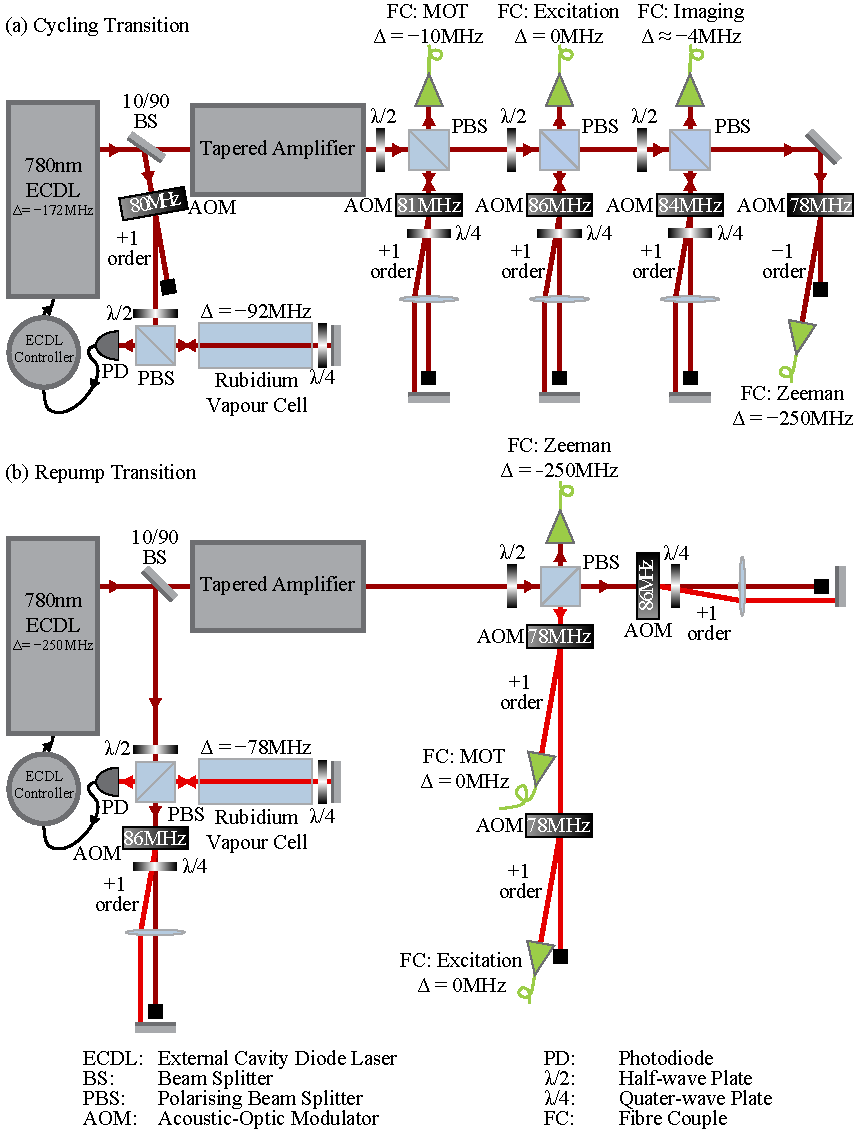
\includegraphics{part2/Figs/laser_setup.pdf}
    \caption{The simplified setup of the lasers locked to the rubidium-85 cycling (a) and repump (b) transitions.
    The \gls{ecdl} lasers are locked with saturated absorption spectroscopy, amplified with tapered amplifiers and offset for numerous applications using acousto-optic modulators.
    $\Delta$s refer to the frequency relative to the cycling or repump transitions.}
    \label{figure:laser_setup}
\end{figure}

\subsection{Rubidium Oven}
The source begins with an effusive Rubidium oven with a long heated collimation tube.
Typically effusive ovens are wasteful with large numbers of atoms lost into a large solid angles however this experimented makes use of a long heated collimation tube to collect and re-emit atoms that were initially emitted at high angles.
These atoms are re-emitted back to the reservoir or into the collimated atom beam leaving the collimation tube.
The rubidium reservoir was typically heated to \unit[80]{$^\circ$C} and the collimation tube to \unit[120]{$^\circ$C}.
A brief schematic of the oven can be found to the left in Figure~\ref{figure:zeemanoven} and more detail on the design, operation, and performance of the oven can be found in References~\cite{bell_slow_2010} and \cite{bell_cold_2011}.

\begin{figure}
    \center
    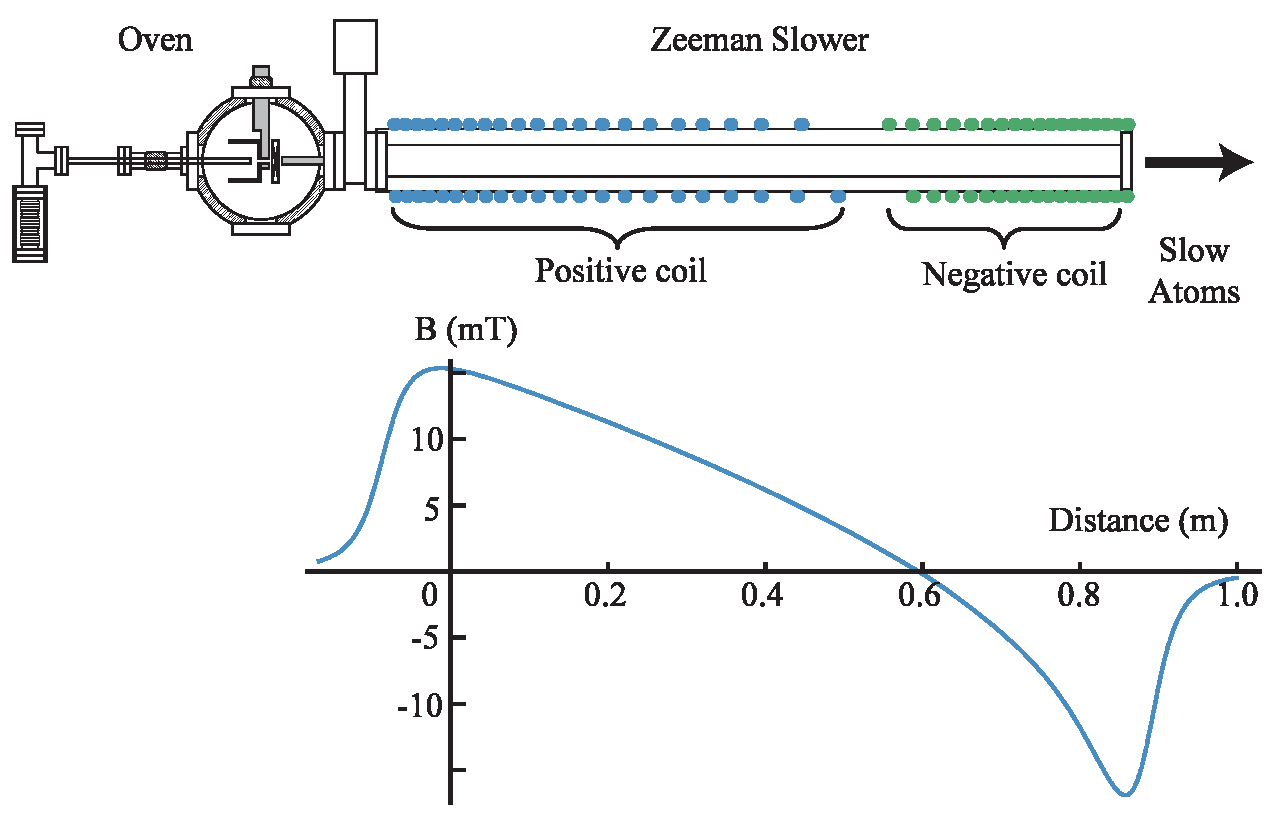
\includegraphics[width=145mm]{part2/Figs/ZeemanOven.pdf}
    \caption{A schematic of the rubidium atom source. Atomic vapour from the oven is directed into the Zeeman slower where a laser detuned from the atomic resonance (shown in red), in combination with a tapered magnetic coil (blue and green), with a magnetic field as shown, slows the thermal atoms.}
    \label{figure:zeemanoven}
\end{figure}

\subsection{Zeeman Slower}
Following the oven is the tapered pitch Zeeman slower which slows atoms down so that they can be captured by the trapping fields of \gls{mot}~\cite{bell_slow_2010}.
Zeeman slowers operate by using a laser red-detuned from resonance to slow the atoms down however as the atoms slow the conditions for resonance change due to the changing Doppler shift.
The solution to this quandary used here is a tapered magnetic coil to apply a magnetic field to shift the atomic resonance such that a particular velocity class of atoms remains resonant with the light field, and thus is slowed, along the length of the Zeeman slower.
Atoms leaving the Zeeman slower typically had velocities around \unit[35]{m/s}, well within the capture velocity of the \gls{mot}.
A schematic of the Zeeman slower with along with the magnetic field produced by the tapered coil is shown in Figure~\ref{figure:zeemanoven}.

When extracting electrons from the \gls{mot} the magnetic coil must be turned off to prevent disruptions to the electron trajectory.

\subsection{Magneto-Optic Trap}
\Glspl{mot} use a combination of magnetic and light fields to trap and cool atoms to $\muup$K temperatures.
In the \gls{caeis} the \gls{mot} was formed from six counter propagating \unit[780]{nm} lasers in a a retro-reflective quasi-mirror \gls{mot} configuration~\cite{hanssen_using_2006,mcculloch_generation_2013} as shown in Figure~\ref{figure:mot} to allow for the accelerator structure consisting of transparent and reflective electrodes.
The magnetic component of the \gls{mot} was formed from two magnetic coils in an anti-Helmholtz configuration providing a zero-field region in the centre of the trap.

The \gls{mot} trapping lasers were detuned \unit[$-10$]{MHz} from the 5$^2$S$_{1/2} $(F=3) $\rightarrow$ 5$^2$P$_{3/2}$ (F$^\prime$=4) Rb85 transition and were mixed with on resonant 5S$_{1/2}$ (F=2) $\rightarrow$ 5P$_{3/2}$ (F$^\prime$=3) light to pump atoms that fell into the dark F=2 state.

\begin{figure}
    \center
    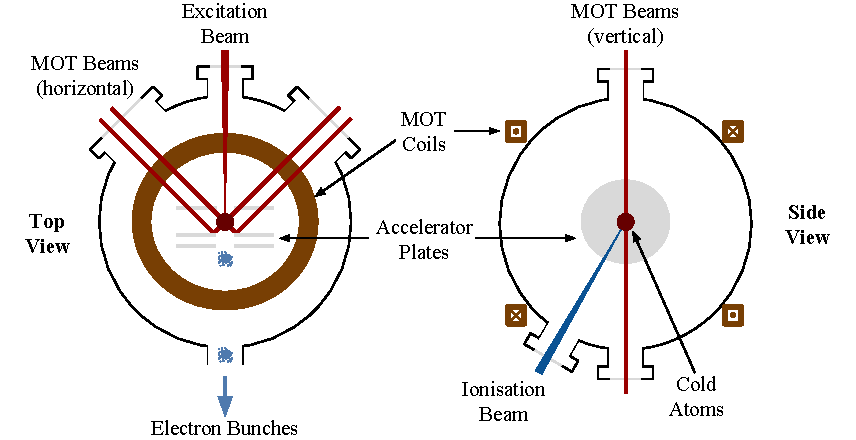
\includegraphics[width=145mm]{part2/Figs/MOTdiagram.pdf}
    \caption{A diagram of the magneto-optic trap, ionisation lasers and accelerator structures.}
    \label{figure:mot}
\end{figure}

\subsection{Ionisation}\label{section:two_stage_ionisation}

The \gls{caes} was capable of generating bunches of electron and ions with long (\unit[$\sim$10]{$\muup$s}), short (\unit[$\sim$5]{ns}), and ultrashort (\unit[$\sim$10]{ps}) bunch duration depending on the laser systems used~\cite{speirs_identification_2017,speirs_electron_2017}.
Depending on the ionisation pathway used, the \gls{caes} was able to produce cold bunches (\unit[$\sim$10]{K}) or hotter bunches (\unit[$>$10]{K}).
Generally cold electron bunches are preferable and bunch duration depends on the desired application, for example \gls{ued} requires ultrashort bunches.

Rubidium has a ground state ionisation threshold of \unit[4.18]{eV} which can be generated using a one blue and one red photon.
The \gls{caeis} has two options for the generation of blue light and two for red.
Red light could be generated by light from a \gls{cw} diode laser amplified by a \gls{ta} and locked to the Rb85 5$^2$S$_{1/2} $(F=3) $\rightarrow$ 5$^2$P$_{3/2} $(F$^\prime$=4) cycling transition or it could be generated with a mode-locked Ti:sapphire amplified pulsed laser with a wavelength range of \unit[770]{nm} to \unit[830]{nm} and a minimum pulse length of \unit[35]{fs}.
Blue light could be generated with a tunable dye pulse laser that produced \unit[460 to 490]{nm} light with a \gls{fwhm} duration of \unit[5]{nm} or with a \gls{cw} laser generated by a high-power tunable frequency-double diode laser.

Sequential ionisation utilised a single red photon to excite from the ground state to an intermediate excited state followed by a single blue photon to transition to a field-ionising state or to the ionisation continuum.
The bunch duration was determined by the shortest of; the duration of the laser pulse driving the transition from the exited state to the ionising state, the lifetime of the intermediate state, or by the depletion time of the intermediate state.

Multiphoton excitation happens when the laser intensities are high enough for nonlinear optical transitions to occur which was the case when the pulse lasers were tightly focused into the atom cloud.
In multiphoton excitation two or more photons are absorbed without transitioning via a real intermediate state.
If $n$ is the number of photon absorbed for the atom to reach its final ionised state then the transition rate is proportional to the $n$th power of the optical intensity~\cite{joachain_atoms_2011}.
Due to the short lifetime of the virtual intermediate states the bunch duration is determined by the duration of the laser pulses.
Multiphoton excitation can occur with just with photons of one colour or with two colour of photons.

Resonance-enhanced multiphoton excitation occurs when a there is a combination of sequential excitation and multiphoton excitation.
Here a number of photons are absorbed to excite the atom to a real intermediate state followed by more photon being absorbed to transition to the final state.
As less photons are required for each transition the overall transition rate can be much higher when compared to plain multiphoton excitation.

\begin{figure}
    \center
    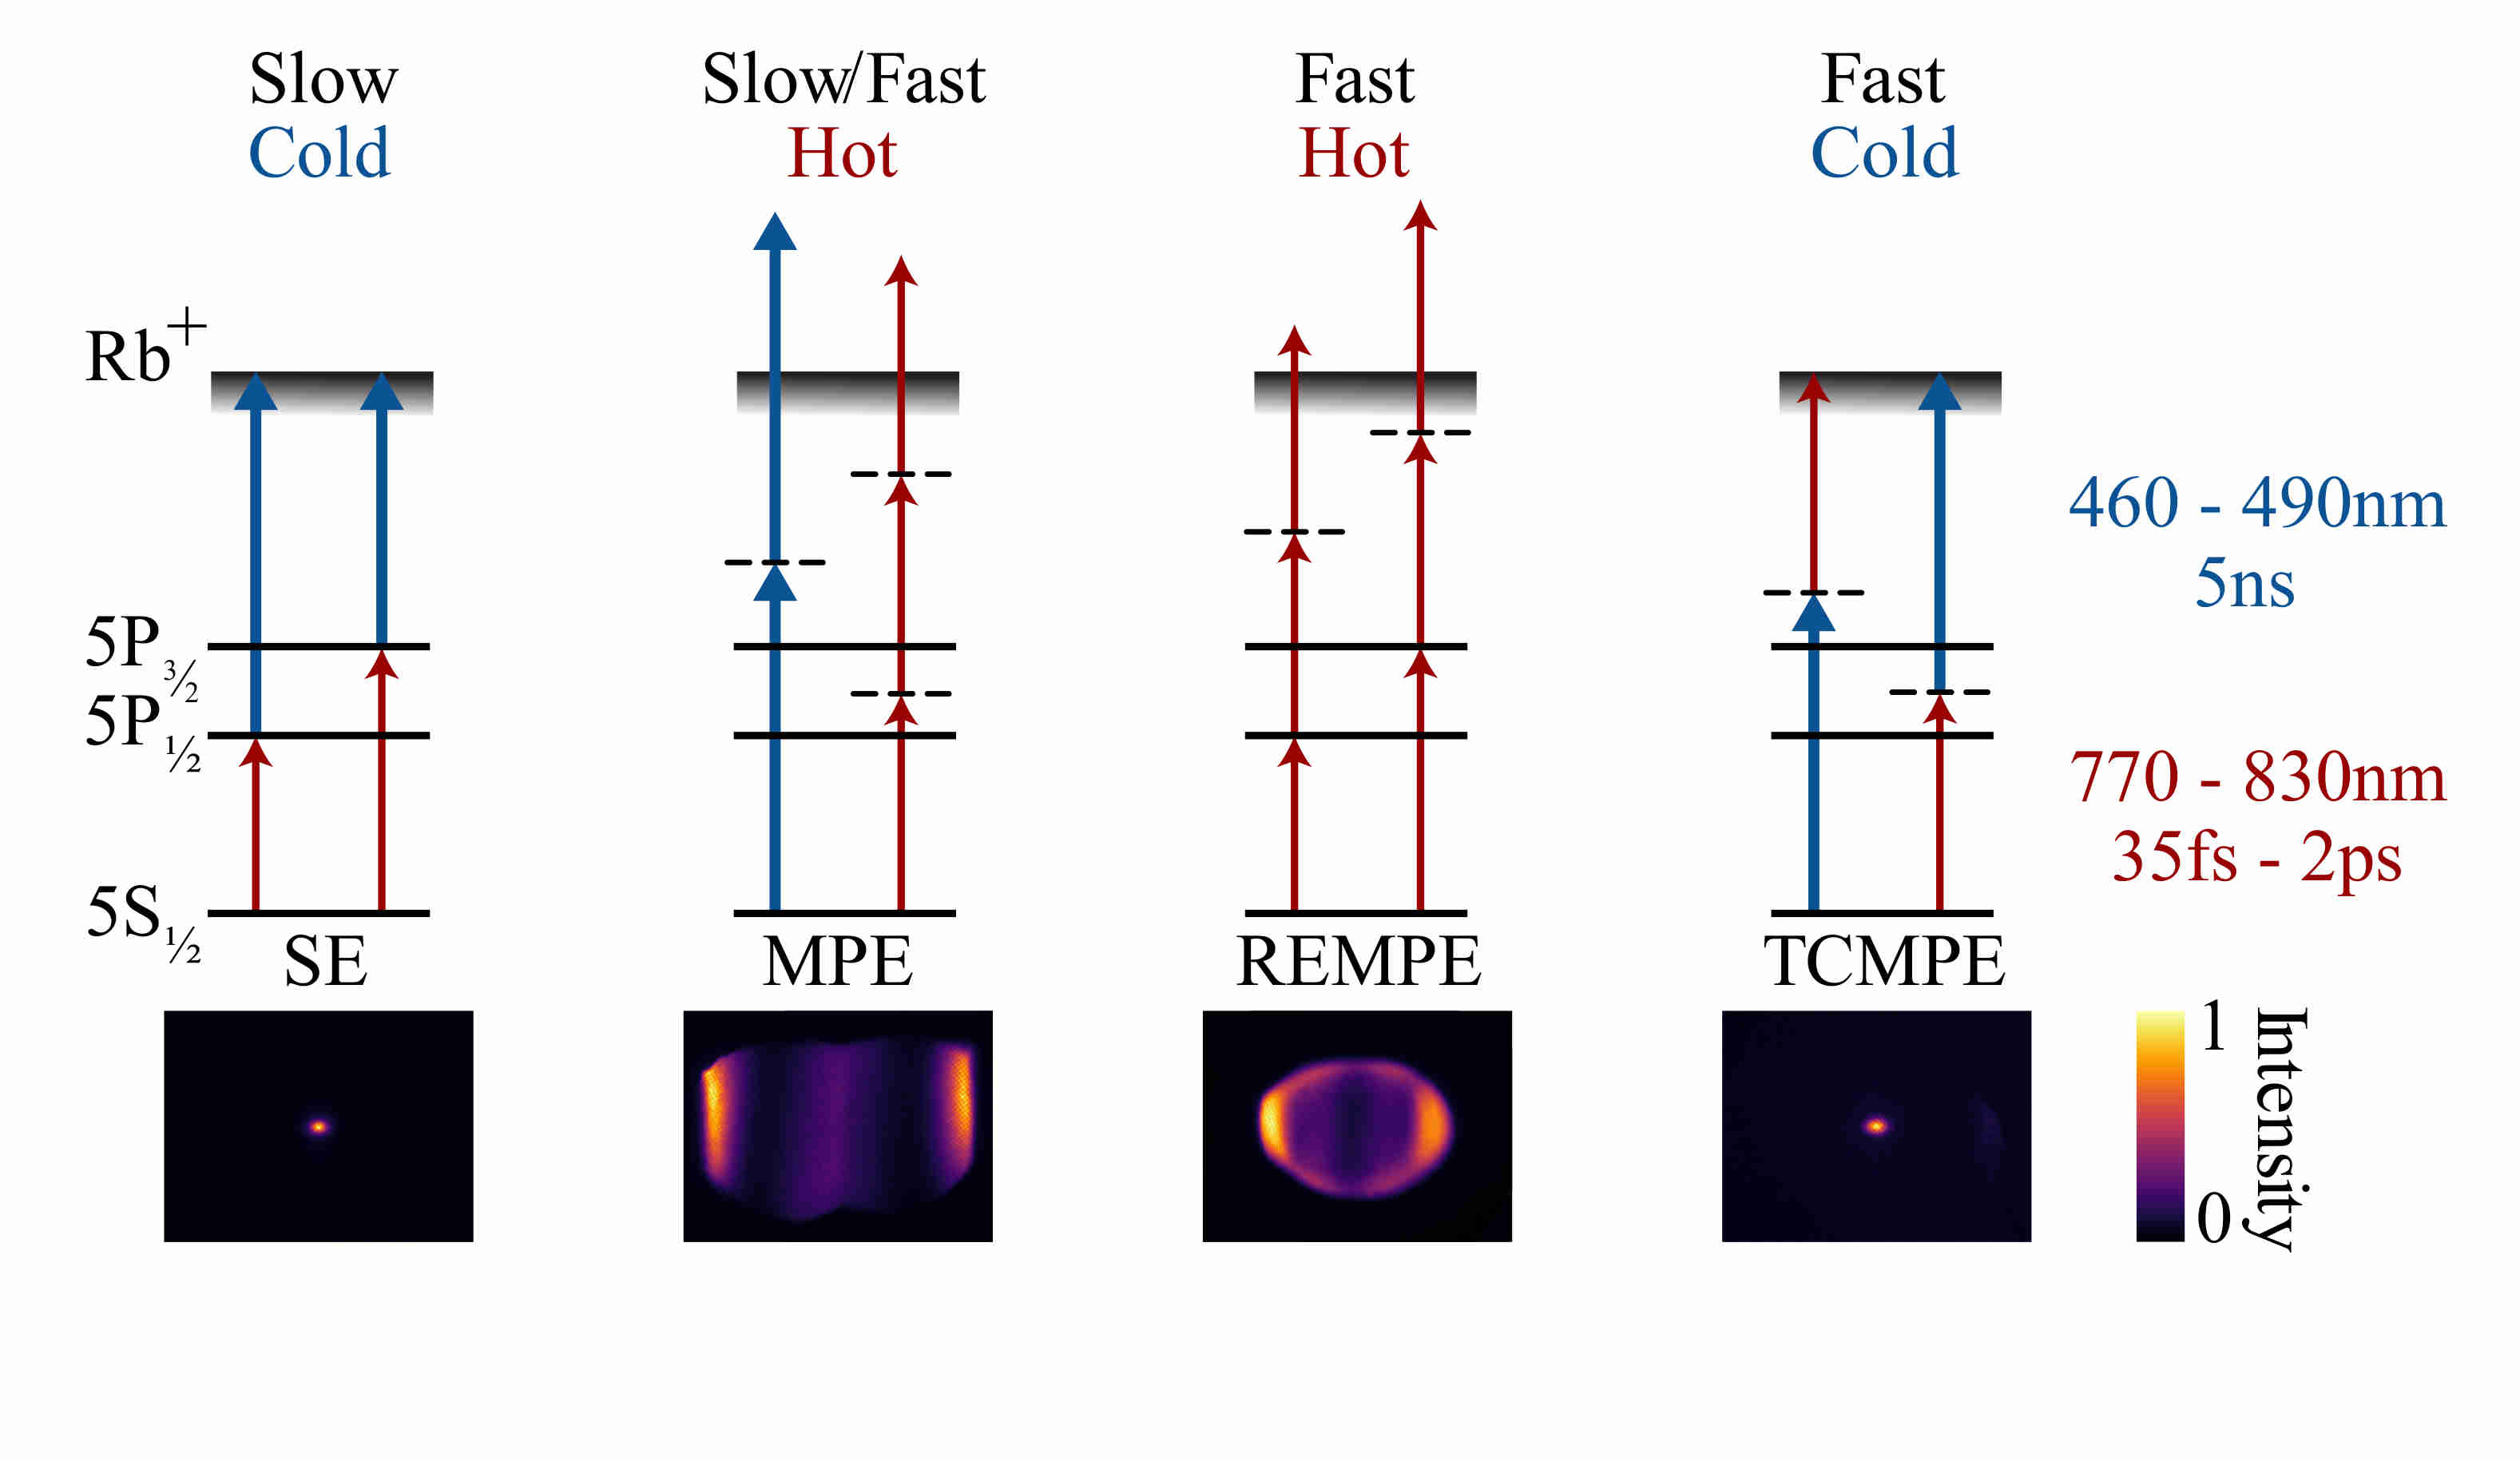
\includegraphics{part2/Figs/ionisationmodes.pdf}
    \caption{A number of photoexcitation pathways were possible in the presence of high intensity illumination by the red a blue lasers in the \gls{caes} such as sequential excitation (SE), multiphoton excitation (MPE), resonance-enhanced multiphoton excitation (REMPE), and two-colour multiphoton excitation (TCMPE). TCMPE is the only pathway that produces bunches that are cold and ultrashort. The images show the transverse momentum distributions for the detected bunches.}
    \label{figure:ionisation_modes}
\end{figure}

The temperature of particles generated from the \gls{caes} depends primarily on the excess ionisation energy given to the atoms by the absorbed photons.
Due to the complex orbits of electrons in high-lying states the relationship between absorbed photon energy and temperature is complex~\cite{mcculloch_high-coherence_2013} but it is generally true that with greater photon energy comes greater source temperature.
The classical ionisation threshold is lower in the presence of electric field, such as the accelerating field in the \gls{caeis}, due to the Stark-shift.
The excess energy of an ion or electron relative to the classical ionisation threshold is:
\begin{equation}\label{equation:ionisation_energy_stark}
\Delta E = -E_I + 2\sqrt{ke^3F} + \sum_{i=0}^{n}{\frac{hc}{\lambda_i}},
\end{equation}
where $E_I=$\,\unit[4.18]{meV} is the ground state ionisation energy of rubidium-85, $k$ is the Coulomb constant, e is the elementary charge, $F$ is the strength of the electric field, $h$ is the Plank constant, and $c$ is speed of light.
The second term represents the Stark-shift of the classical ionisation threshold, and the last term is the sum of the energy of the $n$ photons involved in the ionisation, with wavelength $\lambda_i$.
Equation~\ref{equation:ionisation_energy_stark} assumes that rubidium is hydrogen-like which is a good approximation as long as $E_I \gg 2\sqrt{ke^3F}$.

Sequential excitation and two-colour multiphoton excitation are the only ionisation processing that produced cold electrons as the excess ionisation energy was minimised by tuning the photon energy.
This can be seen in Figure~\ref{figure:ionisation_modes} in the momentum distributions.

Due to the tunability of the lasers involved in generating cold electrons it was possible to directly ionise regardless of the electric field which resulted in short duration bunches, field-ionise such that the majority of the bunch had a short duration but some particles continued to tunnel out over a longer duration, or to excite the atoms such that tunneling through the Stark-shifted potential was the only route to ionisation resulting in lower bunch current and long duration.
The short bunch duration depended on the duration of the laser pulses, generally either the ultrafast bunches with less than \unit[320]{ps} duration using the red femtosecond pulse laser, or \unit[5]{ns} long bunches with \gls{cw} red and the \unit[5]{ns} pulsed blue laser.
Long duration bunch length depended on the lifetime of the atomic states involved and tended to be of order \unit[10]{$\muup$s}~\cite{speirs_identification_2017}.

\subsubsection{Beam Shaping}

The \glspl{caeis} was able to shape the profile of the electron and ion bunches produced by manipulating the red excitation and blue ionisation beam~\cite{mcculloch_arbitrarily_2011}.
The lasers imparted their profiles onto the ionised atoms which, for cold low-emittance bunches, could be maintained to the detector.
The transverse bunch profile was determined by the red excitation laser profile combined with the density profile of the atomic cloud.
Similarly the longitudinal profile depended on the ionisation laser profile and atomic cloud density.
Beam shaping required the red and blue lasers to not be saturating the atomic cloud.

Control over the excitation beam profile was achieved with a \gls{slm} and an iterative feedback system~\cite{van_bijnen_patterned_2015}.
With a second \gls{slm} and control system the longitudinal profile could also be controllable.
A schematic of the bunch profile system is shown in Figure~\ref{figure:beam_shaping_schematic} and an example of its performance can be seen in Figure~\ref{figure:beam_shaping}.

\begin{figure}
    \center
    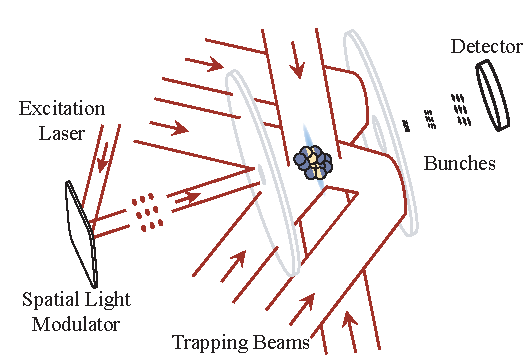
\includegraphics{part2/Figs/beam_shaping_schem.pdf}
    \caption{A schematic of the shaping apparatus. The excitation laser pulse is shaped with a \gls{slm} to form an arbitrary beam profile at the atom cloud, imparting that profile onto the bunch produced by the \gls{caeis}. In this diagram the blue ionisation laser comes from behind the atom cloud.}
    \label{figure:beam_shaping_schematic}
\end{figure}

\begin{figure}
    \center
    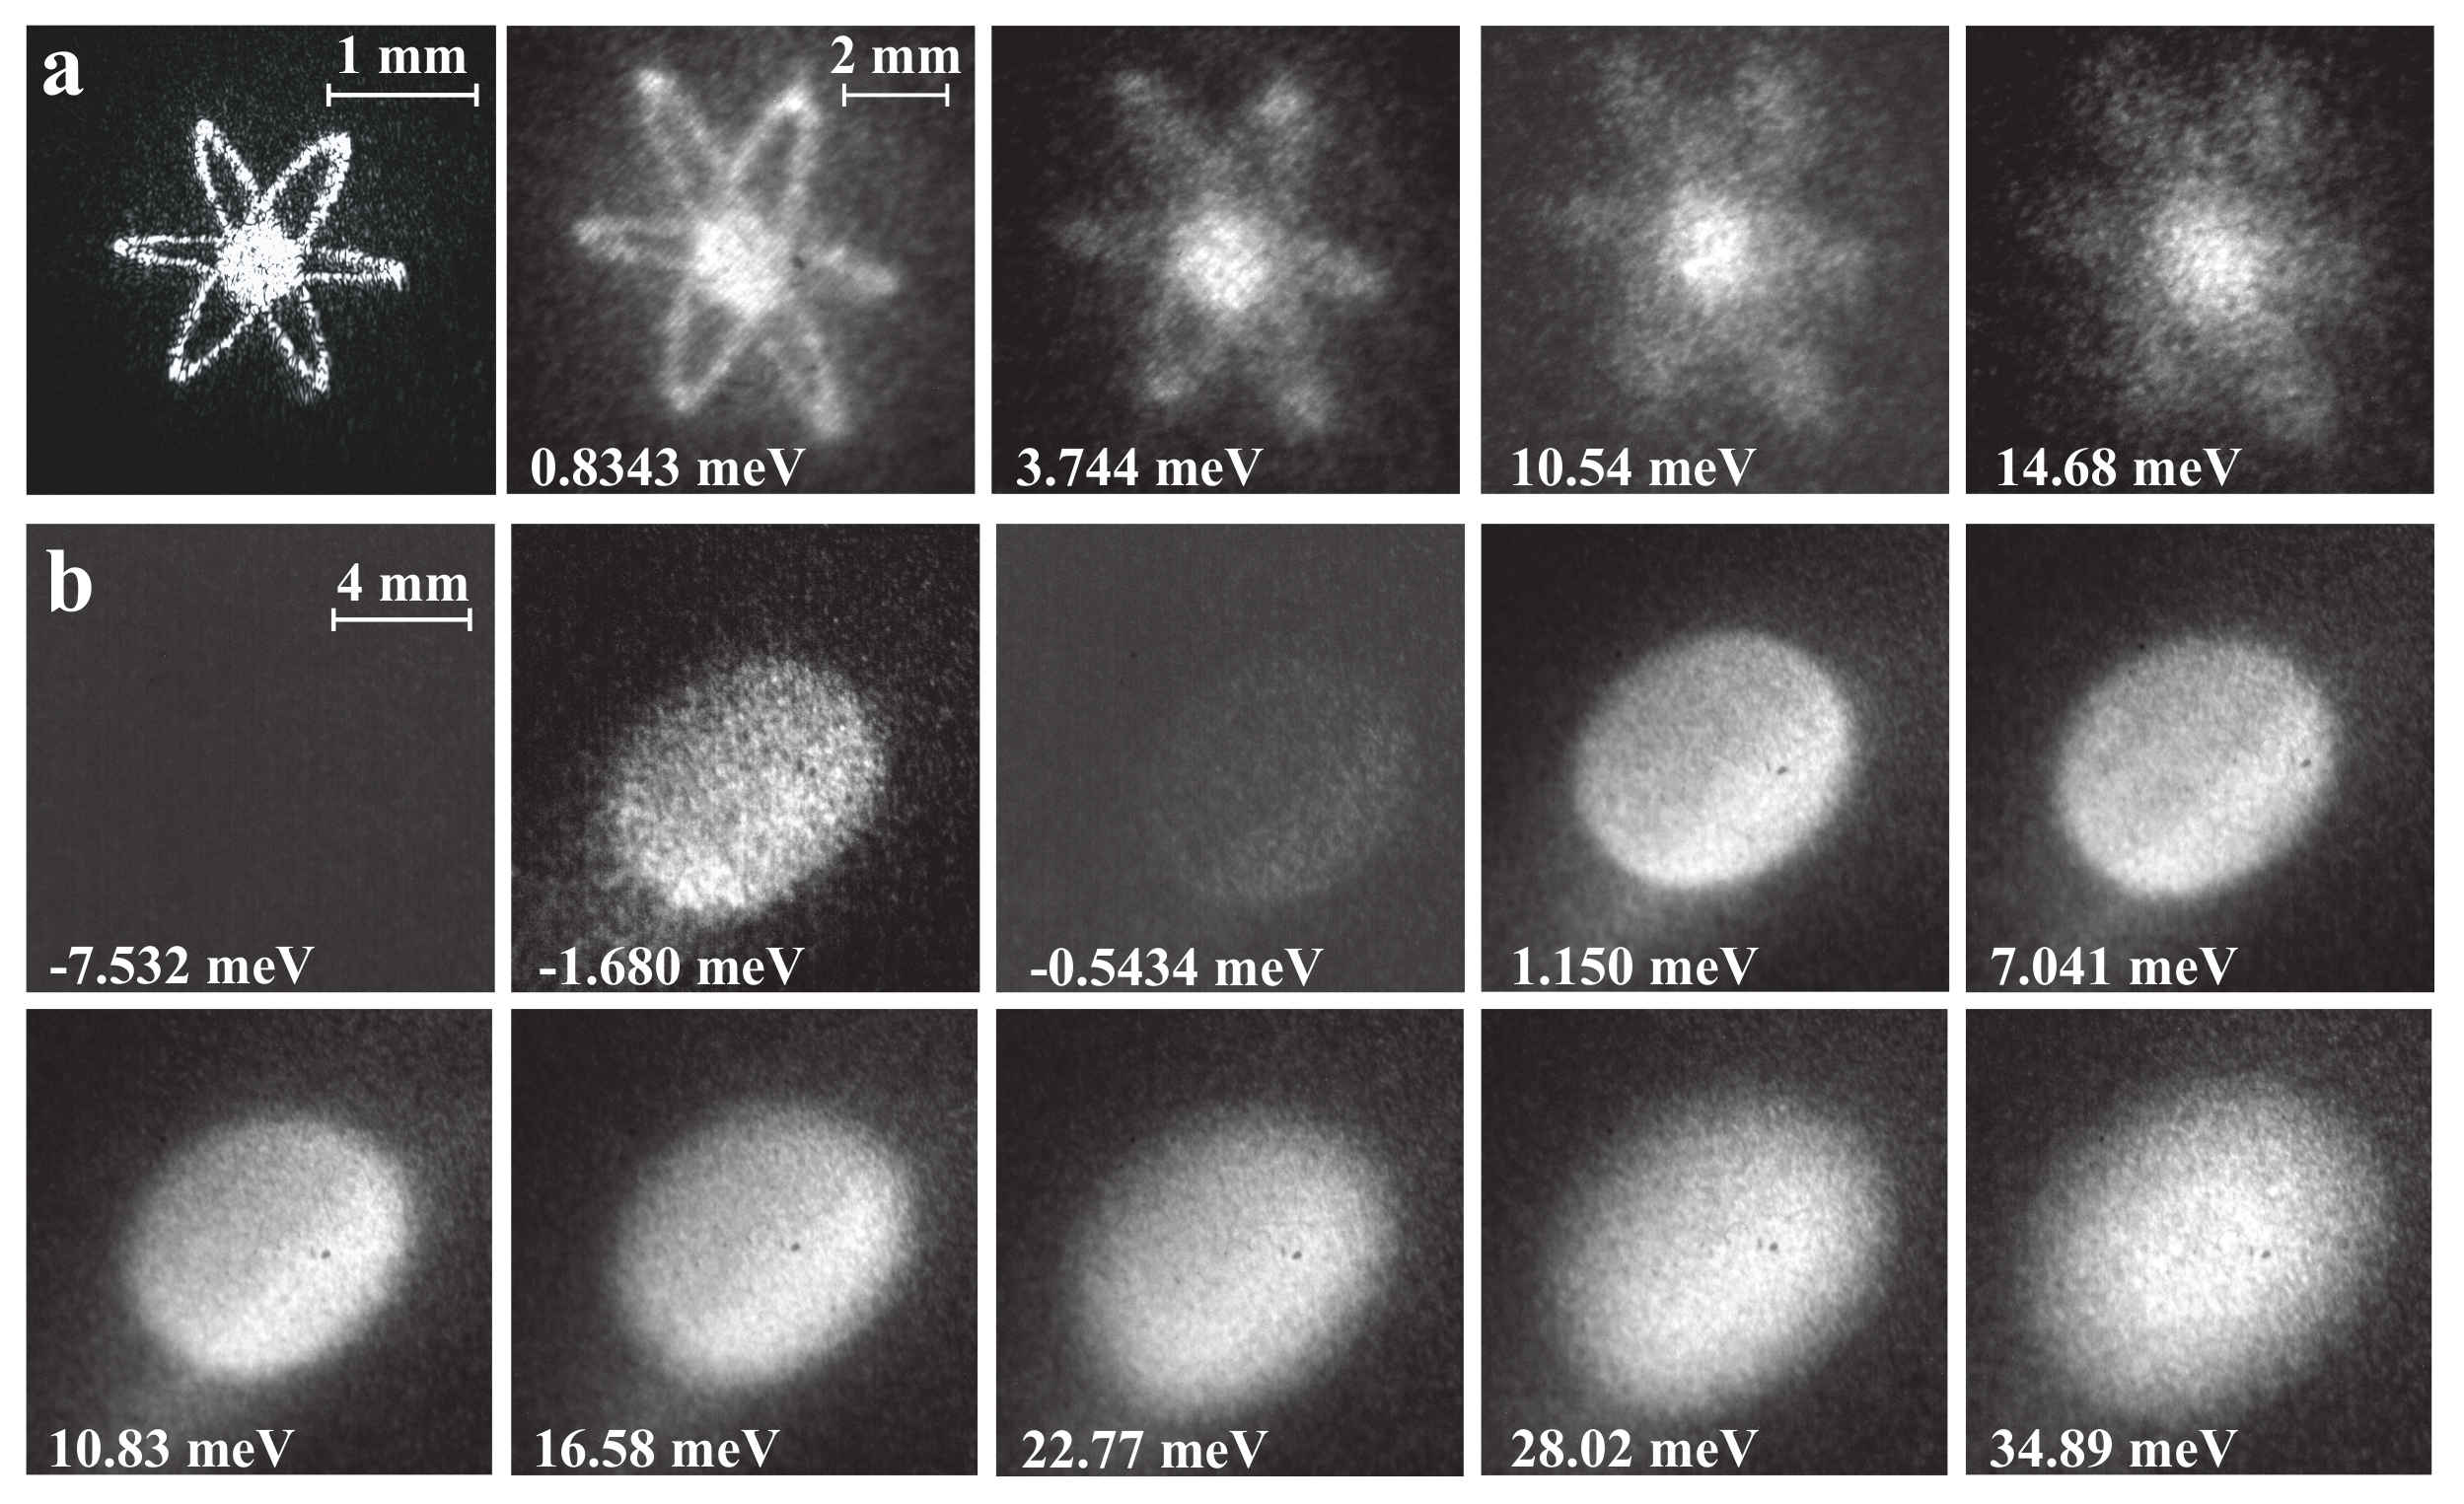
\includegraphics{part2/Figs/beam_shaping.pdf}
    \caption{An example of beam shaping and the effects of temperature on the degradation of the bunch profile.
    \emph{a} Excitation laser profile (left), followed by detected electron bunches as excess ionisation energy is varied.
    \emph{b} Electron bunches generated from a uniform excitation laser profile as excess energy is varied.
    At \unit[-1.680]{meV} bunch current increases as the ionisation laser couples to a Rydberg state.}
    \label{figure:beam_shaping}
\end{figure}

Control over the bunch profile allows for customisation and feedback for whatever application the \gls{caeis} is being used for but is of particular interest for countering space-charge expansion.
With the bunch charges achieved to date only the ultrashort duration bunches are dense enough to experience significant space-charge expansion which degrades the coherence and emittance of the beam and is thus detrimental to imaging applications.
Suppression of space-charge expansion has been demonstrated with the \gls{caeis} by beam shaping~\cite{luiten_how_2004,thompson_suppression_2016}.

\subsection{Accelerator}

The static accelerating electric field was generated by two accelerator electrodes which were approximately \unit[11]{cm} in diameter and \unit[4]{mm} thick with the transmissive plate being \gls{ar} coated at \unit[780]{nm} and coated with indium-tin-oxide which is also transmisive to \unit[780]{nm} to 96\%.
The second reflective electrode was composed of copper coated with polished gold and there was a third electrode that was not consistently used.
Each of the electrodes had an aperture in the center to allow the electron and ion bunches to pass through.

The limit to the beam energy the apperatus was able to produce was determined by the maximum voltages that could be applied to the electrodes, any higher and the electrodes would begin to either arc or short.

\subsection{Beam Optics}

There were a number of systems in place for manipulating the electron and ion beams; a solenoid lens, an Einzel lens, a magnetic quadrupole lens, a one-axis deflector, and a number of permanent magnets located outside the vacuum system.
The lenses were used to focus the bunches, usually to a focus on the detector but sometimes to manipulate the size of the beam at the sample plane.
The quadrupole lens was used to counter astigmatism in the beam and is discussed in more detail in Section~\ref{section:quadrupole}.
The deflector was located after the sample stage and was used to streak bunches across the detector.
The permanent magnets were used to steer electron bunches through the system, through a number of apertures and countering the deflection imposed by a number of anomalous magnetic fields present with the \gls{caeis}.

\subsection{Sample Management}

Experimental samples were mounted on a custom sample mount formed from an aluminium paddle that was large enough to mount eight \gls{tem} samples and block any portion of the beam not passing through the samples.
The samples were held by two commercial \gls{tem} mounts attached to the paddle that were able to fit \unit[3.05]{mm} diameter samples with approximately \unit[2]{mm} diameter of the sample visible to the bunches when the sample lid was in place.
Grazing incidence reflection diffraction samples could also be mounted at the end of the paddle as shown in Figure~\ref{figure:sample_holder}.
The sample paddle was mounted on a stage with manual control over two-axis translation transverse to the beam axis and rotation.
The sample paddle could also be connected to a high-voltage supply to allow for the sample to be biased to further manipulate the beam energy as described in Section~\ref{section:sample_bias}.

\begin{figure}
    \centering
    \begin{subfigure}{0.49\linewidth}
    \centering
    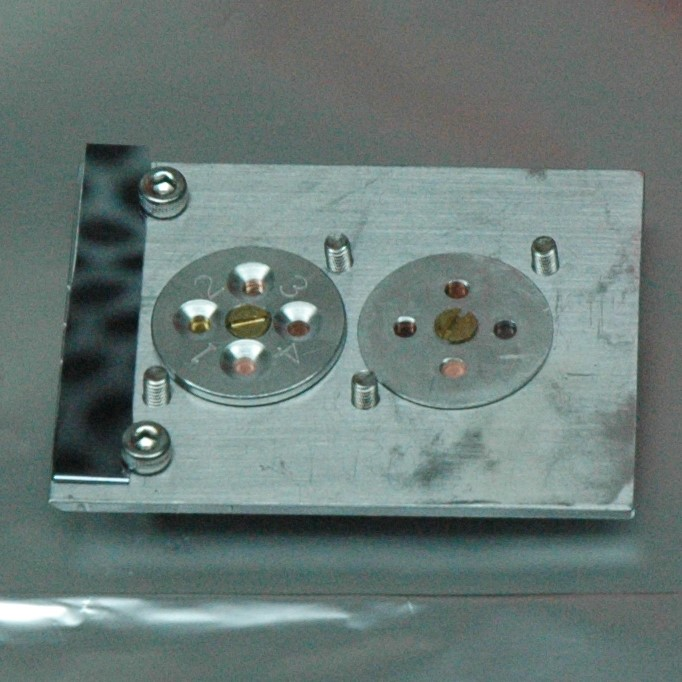
\includegraphics[width=\linewidth]{part2/Figs/sample_holder_alone.jpg}
    \end{subfigure}
    \begin{subfigure}{0.49\linewidth}
    \centering
    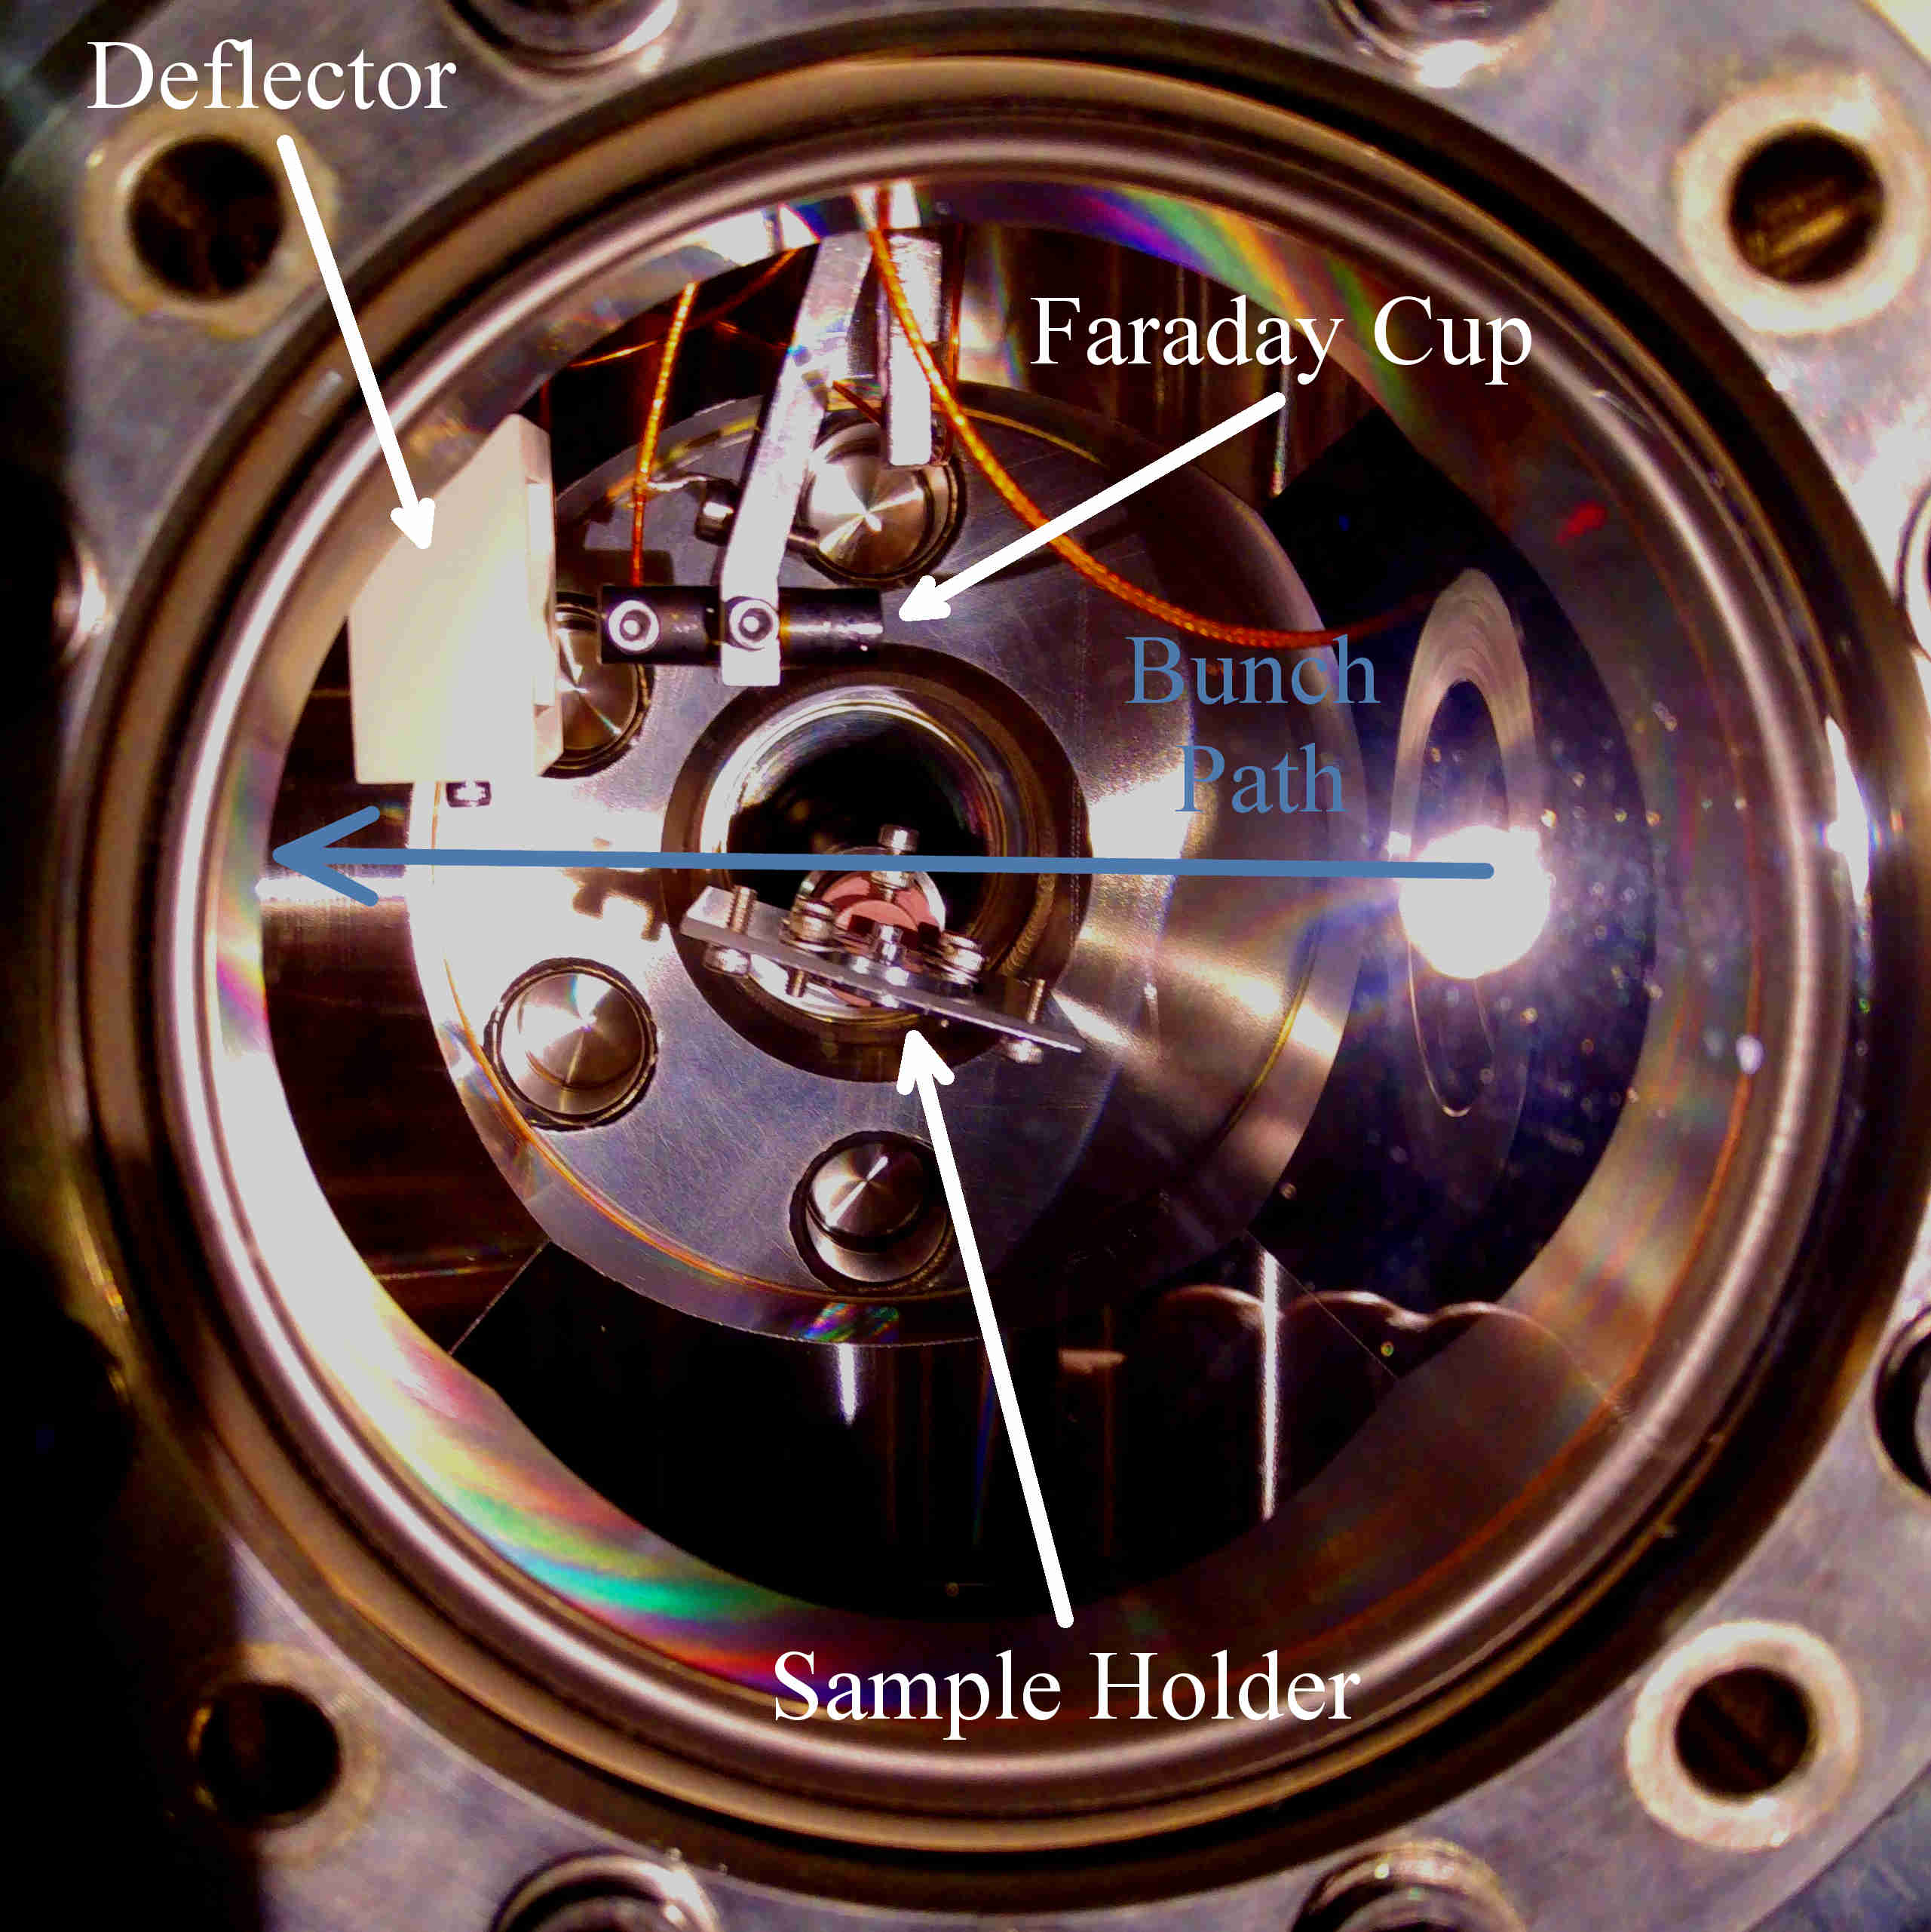
\includegraphics[width=\linewidth]{part2/Figs/sample_holder_in_vitro.jpg}
    \end{subfigure}
    \caption{The sample holder used in the \gls{caes}. In the left photograph the sample holder with eight transmission samples and a reflection sample is shown. On the right is the sample holder in the sample chamber, with the post-sample deflector and Faraday cup also visible retracted from the beam path (bunches travel from right to left).}
    \label{figure:sample_holder}
\end{figure}

\subsection{Timing}\label{section:pulse_blaster}

Synchronisation throughout the experiment was achieved with a 24-channel digital timing card\footnote{Spincore Pulseblaster PCI mounted in external USB enclosure.}.
Low voltage TTL signals are used to trigger the numerous time-sensitive devices involved in the experiment.
The \gls{caeis} operated at the frequency of the flashlamp of the \unit[5]{ns} blue pulse laser, \unit[10]{Hz}.
The sequence began with \gls{mot} and Zeeman lasers and fields turning on to load the trap for approximately \unit[90]{ms}.
The trapping lasers and fields were extinguished \unit[5]{ms} before the excitation and ionisation lasers and \gls{ccd} camera were triggered to generate and detect the electron or ion bunch.

\section{Current Limitations}

There were a number of factors preventing the \gls{caeis} achieving its goal of single-shot ultrafast electron diffractive imaging, most importantly electron flux and beam stability.
These factors also require improvement for other \gls{caes} goals such as \gls{fib} milling, and imaging.

The minimum electron flux required for \gls{ued} is 10$^6$ electrons per bunch~\cite{van_oudheusden_compression_2010} whereas this iteration of the \gls{caes} was only able to get $5\times10^5$ electrons at best.
There are a few avenues available to the \gls{caeis} to improve the bunch count such as increasing the \gls{mot} density, increasing the power of the ionisation laser, better optimisation of the ionisation pathways~\cite{mcculloch_field_2017}, and potentially running the apparatus in \gls{cw} mode.
\Gls{cw} mode  has the potential to increase the number of particles per second however some applications would be difficult or impossible without discrete bunches.
An investigation of the performance of the apparatus in \gls{cw} mode is shown in Section\ref{section:pulse_vs_continuous}.

The stability of the source was also problematic, particularly for electron bunches, as a number of transient effects interfered with the path of the beams on timescales from shot-to-shot to minute-to-minute.
Effects such as eddy currents due to the switching of the strong magnetic fields in the steel of the vacuum system and optical tables was one of the primary suspects for a source of the perturbations in the beam path.
Other potential sources are the electronic equipment such as power supplies and switches that were placed as far away from the beam path as practical but were still in the vicinity.
The poor stability of the source made some measurements difficult and others impossible.
Multi-shot measurements were required in a number of cases and, due to the drift of the beam, straight averages of the images from the detector resulted in a unusable blur.
Generating usable images for multi-shot measurements required `registration' of the images, set averages where the features in each individual image was aligned with the other images to prevent blurring.
Measurements without sharp features could not be well registered, as the registration algorithms have trouble precisely aligning the images.
Registration is discussed further in Section~\ref{section:registration}.

\section{Pulsed vs Continuous}\label{section:pulse_vs_continuous}
Comparing the performance of the source in its usual pulse mode against the performance as a continuous source had the potential to show pathways for improving the pulsed mode as well as providing an alternative that could provide better performance for particular applications, as some measurements, such as simple \gls{cdi}, do not require the source to be pulsed.
Continuous mode functions by using the two-stage ionisation and acceleration on the atom beam from the oven without cooling or trapping by the Zeeman slower or \gls{mot}.
It was hoped that the beam current would increase with this mode of operation and that the beam produced would be subject to less drift and instability as the large magnetic fields were not switching.

While the entire apparatus and control system had been designed to operate in pulse mode it was fortunately relatively simple to modify the setup to operate continuously.
The \gls{mot} was disabled, the excitation beam was left on, and the \gls{cw} blue was used instead of the usual blue pulse laser to act as the ionisation laser.

Before switching to continuous mode the \gls{caeis} had been measured to have \unit[$0.42\times10^6$]{electrons per bunch} equating to a beam current of \unit[$4.2\times10^6$]{electrons per second}.
Initially the continuous mode was producing \unit[$0.64\times10^6$]{electrons per second} however there were a number of optimisations available to improve the current, as detailed below.

\subsection{Oven Temperature to Electron Count}
When operating in pulsed mode the \gls{mot} was given more than enough time to saturate and thus there was no benefit to producing more electrons from the oven.
In continuous mode the beam current was dependent on the density of atoms in the ionisation region which could be increased by producing more atoms from the oven.

The atomic flux from the oven could be increased by running the oven at a higher temperature.
During normal operation the oven was set to a temperature of approximately \unit[80]{$^\circ$C} (rubidium has a melting point of \unit[39.30]{$^\circ$C}) however the oven is able to operate at up to \unit[200]{$^\circ$C}.

{\color{red}Atomic flux from oven vs temperature??}

The effects of the oven temperature on the beam current are shown in Figure~\ref{figure:oven_counts}.
There was a significant increase in the beam current as the oven temperature was increased, with a high enough temperature is was even greater than that of the pulsed mode bunches.
The unfortunate side affect of running the oven at such high temperatures is that the lifetime of the \unit[5]{g} rubidium ampule in the oven will be drastically reduced to the point where a threefold increase in current is not worth the reduced lifetime.
This data indicates that the \gls{cw} beam current could be improved with the use of transverse compression of the atom beam which would provide a similar improvement to beam current as more atoms would be present in the ionisation region~\cite{tielen_development_2015}.

\begin{figure}
    \center
    %% Creator: Matplotlib, PGF backend
%%
%% To include the figure in your LaTeX document, write
%%   \input{<filename>.pgf}
%%
%% Make sure the required packages are loaded in your preamble
%%   \usepackage{pgf}
%%
%% Figures using additional raster images can only be included by \input if
%% they are in the same directory as the main LaTeX file. For loading figures
%% from other directories you can use the `import` package
%%   \usepackage{import}
%% and then include the figures with
%%   \import{<path to file>}{<filename>.pgf}
%%
%% Matplotlib used the following preamble
%%
\begingroup%
\makeatletter%
\begin{pgfpicture}%
\pgfpathrectangle{\pgfpointorigin}{\pgfqpoint{4.282500in}{2.141250in}}%
\pgfusepath{use as bounding box, clip}%
\begin{pgfscope}%
\pgfsetbuttcap%
\pgfsetmiterjoin%
\definecolor{currentfill}{rgb}{1.000000,1.000000,1.000000}%
\pgfsetfillcolor{currentfill}%
\pgfsetlinewidth{0.000000pt}%
\definecolor{currentstroke}{rgb}{1.000000,1.000000,1.000000}%
\pgfsetstrokecolor{currentstroke}%
\pgfsetdash{}{0pt}%
\pgfpathmoveto{\pgfqpoint{0.000000in}{0.000000in}}%
\pgfpathlineto{\pgfqpoint{4.282500in}{0.000000in}}%
\pgfpathlineto{\pgfqpoint{4.282500in}{2.141250in}}%
\pgfpathlineto{\pgfqpoint{0.000000in}{2.141250in}}%
\pgfpathclose%
\pgfusepath{fill}%
\end{pgfscope}%
\begin{pgfscope}%
\pgfsetbuttcap%
\pgfsetmiterjoin%
\definecolor{currentfill}{rgb}{1.000000,1.000000,1.000000}%
\pgfsetfillcolor{currentfill}%
\pgfsetlinewidth{0.000000pt}%
\definecolor{currentstroke}{rgb}{0.000000,0.000000,0.000000}%
\pgfsetstrokecolor{currentstroke}%
\pgfsetstrokeopacity{0.000000}%
\pgfsetdash{}{0pt}%
\pgfpathmoveto{\pgfqpoint{0.691823in}{0.532919in}}%
\pgfpathlineto{\pgfqpoint{4.028722in}{0.532919in}}%
\pgfpathlineto{\pgfqpoint{4.028722in}{1.926770in}}%
\pgfpathlineto{\pgfqpoint{0.691823in}{1.926770in}}%
\pgfpathclose%
\pgfusepath{fill}%
\end{pgfscope}%
\begin{pgfscope}%
\pgfpathrectangle{\pgfqpoint{0.691823in}{0.532919in}}{\pgfqpoint{3.336899in}{1.393852in}} %
\pgfusepath{clip}%
\pgfsetrectcap%
\pgfsetroundjoin%
\pgfsetlinewidth{1.003750pt}%
\definecolor{currentstroke}{rgb}{0.309804,0.478431,0.682353}%
\pgfsetstrokecolor{currentstroke}%
\pgfsetdash{}{0pt}%
\pgfpathmoveto{\pgfqpoint{1.029684in}{0.596936in}}%
\pgfpathlineto{\pgfqpoint{1.584443in}{0.629190in}}%
\pgfpathlineto{\pgfqpoint{2.270593in}{0.845827in}}%
\pgfpathlineto{\pgfqpoint{2.650166in}{1.273641in}}%
\pgfpathlineto{\pgfqpoint{2.825353in}{1.276714in}}%
\pgfpathlineto{\pgfqpoint{3.238294in}{1.418479in}}%
\pgfpathlineto{\pgfqpoint{3.667920in}{1.479532in}}%
\pgfpathlineto{\pgfqpoint{3.903588in}{1.780648in}}%
\pgfusepath{stroke}%
\end{pgfscope}%
\begin{pgfscope}%
\pgfpathrectangle{\pgfqpoint{0.691823in}{0.532919in}}{\pgfqpoint{3.336899in}{1.393852in}} %
\pgfusepath{clip}%
\pgfsetbuttcap%
\pgfsetroundjoin%
\pgfsetlinewidth{1.003750pt}%
\definecolor{currentstroke}{rgb}{0.000000,0.000000,0.000000}%
\pgfsetstrokecolor{currentstroke}%
\pgfsetdash{{6.000000pt}{6.000000pt}}{0.000000pt}%
\pgfpathmoveto{\pgfqpoint{0.691823in}{0.951074in}}%
\pgfpathlineto{\pgfqpoint{4.028722in}{0.951074in}}%
\pgfusepath{stroke}%
\end{pgfscope}%
\begin{pgfscope}%
\pgfsetrectcap%
\pgfsetmiterjoin%
\pgfsetlinewidth{1.003750pt}%
\definecolor{currentstroke}{rgb}{0.000000,0.000000,0.000000}%
\pgfsetstrokecolor{currentstroke}%
\pgfsetdash{}{0pt}%
\pgfpathmoveto{\pgfqpoint{4.028722in}{0.532919in}}%
\pgfpathlineto{\pgfqpoint{4.028722in}{1.926770in}}%
\pgfusepath{stroke}%
\end{pgfscope}%
\begin{pgfscope}%
\pgfsetrectcap%
\pgfsetmiterjoin%
\pgfsetlinewidth{1.003750pt}%
\definecolor{currentstroke}{rgb}{0.000000,0.000000,0.000000}%
\pgfsetstrokecolor{currentstroke}%
\pgfsetdash{}{0pt}%
\pgfpathmoveto{\pgfqpoint{0.691823in}{0.532919in}}%
\pgfpathlineto{\pgfqpoint{0.691823in}{1.926770in}}%
\pgfusepath{stroke}%
\end{pgfscope}%
\begin{pgfscope}%
\pgfsetrectcap%
\pgfsetmiterjoin%
\pgfsetlinewidth{1.003750pt}%
\definecolor{currentstroke}{rgb}{0.000000,0.000000,0.000000}%
\pgfsetstrokecolor{currentstroke}%
\pgfsetdash{}{0pt}%
\pgfpathmoveto{\pgfqpoint{0.691823in}{1.926770in}}%
\pgfpathlineto{\pgfqpoint{4.028722in}{1.926770in}}%
\pgfusepath{stroke}%
\end{pgfscope}%
\begin{pgfscope}%
\pgfsetrectcap%
\pgfsetmiterjoin%
\pgfsetlinewidth{1.003750pt}%
\definecolor{currentstroke}{rgb}{0.000000,0.000000,0.000000}%
\pgfsetstrokecolor{currentstroke}%
\pgfsetdash{}{0pt}%
\pgfpathmoveto{\pgfqpoint{0.691823in}{0.532919in}}%
\pgfpathlineto{\pgfqpoint{4.028722in}{0.532919in}}%
\pgfusepath{stroke}%
\end{pgfscope}%
\begin{pgfscope}%
\pgfsetbuttcap%
\pgfsetroundjoin%
\definecolor{currentfill}{rgb}{0.000000,0.000000,0.000000}%
\pgfsetfillcolor{currentfill}%
\pgfsetlinewidth{0.501875pt}%
\definecolor{currentstroke}{rgb}{0.000000,0.000000,0.000000}%
\pgfsetstrokecolor{currentstroke}%
\pgfsetdash{}{0pt}%
\pgfsys@defobject{currentmarker}{\pgfqpoint{0.000000in}{0.000000in}}{\pgfqpoint{0.000000in}{0.055556in}}{%
\pgfpathmoveto{\pgfqpoint{0.000000in}{0.000000in}}%
\pgfpathlineto{\pgfqpoint{0.000000in}{0.055556in}}%
\pgfusepath{stroke,fill}%
}%
\begin{pgfscope}%
\pgfsys@transformshift{0.691823in}{0.532919in}%
\pgfsys@useobject{currentmarker}{}%
\end{pgfscope}%
\end{pgfscope}%
\begin{pgfscope}%
\pgfsetbuttcap%
\pgfsetroundjoin%
\definecolor{currentfill}{rgb}{0.000000,0.000000,0.000000}%
\pgfsetfillcolor{currentfill}%
\pgfsetlinewidth{0.501875pt}%
\definecolor{currentstroke}{rgb}{0.000000,0.000000,0.000000}%
\pgfsetstrokecolor{currentstroke}%
\pgfsetdash{}{0pt}%
\pgfsys@defobject{currentmarker}{\pgfqpoint{0.000000in}{-0.055556in}}{\pgfqpoint{0.000000in}{0.000000in}}{%
\pgfpathmoveto{\pgfqpoint{0.000000in}{0.000000in}}%
\pgfpathlineto{\pgfqpoint{0.000000in}{-0.055556in}}%
\pgfusepath{stroke,fill}%
}%
\begin{pgfscope}%
\pgfsys@transformshift{0.691823in}{1.926770in}%
\pgfsys@useobject{currentmarker}{}%
\end{pgfscope}%
\end{pgfscope}%
\begin{pgfscope}%
\pgftext[x=0.691823in,y=0.477363in,,top]{\fontsize{10.000000}{12.000000}\selectfont \(\displaystyle 60\)}%
\end{pgfscope}%
\begin{pgfscope}%
\pgfsetbuttcap%
\pgfsetroundjoin%
\definecolor{currentfill}{rgb}{0.000000,0.000000,0.000000}%
\pgfsetfillcolor{currentfill}%
\pgfsetlinewidth{0.501875pt}%
\definecolor{currentstroke}{rgb}{0.000000,0.000000,0.000000}%
\pgfsetstrokecolor{currentstroke}%
\pgfsetdash{}{0pt}%
\pgfsys@defobject{currentmarker}{\pgfqpoint{0.000000in}{0.000000in}}{\pgfqpoint{0.000000in}{0.055556in}}{%
\pgfpathmoveto{\pgfqpoint{0.000000in}{0.000000in}}%
\pgfpathlineto{\pgfqpoint{0.000000in}{0.055556in}}%
\pgfusepath{stroke,fill}%
}%
\begin{pgfscope}%
\pgfsys@transformshift{1.108935in}{0.532919in}%
\pgfsys@useobject{currentmarker}{}%
\end{pgfscope}%
\end{pgfscope}%
\begin{pgfscope}%
\pgfsetbuttcap%
\pgfsetroundjoin%
\definecolor{currentfill}{rgb}{0.000000,0.000000,0.000000}%
\pgfsetfillcolor{currentfill}%
\pgfsetlinewidth{0.501875pt}%
\definecolor{currentstroke}{rgb}{0.000000,0.000000,0.000000}%
\pgfsetstrokecolor{currentstroke}%
\pgfsetdash{}{0pt}%
\pgfsys@defobject{currentmarker}{\pgfqpoint{0.000000in}{-0.055556in}}{\pgfqpoint{0.000000in}{0.000000in}}{%
\pgfpathmoveto{\pgfqpoint{0.000000in}{0.000000in}}%
\pgfpathlineto{\pgfqpoint{0.000000in}{-0.055556in}}%
\pgfusepath{stroke,fill}%
}%
\begin{pgfscope}%
\pgfsys@transformshift{1.108935in}{1.926770in}%
\pgfsys@useobject{currentmarker}{}%
\end{pgfscope}%
\end{pgfscope}%
\begin{pgfscope}%
\pgftext[x=1.108935in,y=0.477363in,,top]{\fontsize{10.000000}{12.000000}\selectfont \(\displaystyle 80\)}%
\end{pgfscope}%
\begin{pgfscope}%
\pgfsetbuttcap%
\pgfsetroundjoin%
\definecolor{currentfill}{rgb}{0.000000,0.000000,0.000000}%
\pgfsetfillcolor{currentfill}%
\pgfsetlinewidth{0.501875pt}%
\definecolor{currentstroke}{rgb}{0.000000,0.000000,0.000000}%
\pgfsetstrokecolor{currentstroke}%
\pgfsetdash{}{0pt}%
\pgfsys@defobject{currentmarker}{\pgfqpoint{0.000000in}{0.000000in}}{\pgfqpoint{0.000000in}{0.055556in}}{%
\pgfpathmoveto{\pgfqpoint{0.000000in}{0.000000in}}%
\pgfpathlineto{\pgfqpoint{0.000000in}{0.055556in}}%
\pgfusepath{stroke,fill}%
}%
\begin{pgfscope}%
\pgfsys@transformshift{1.526048in}{0.532919in}%
\pgfsys@useobject{currentmarker}{}%
\end{pgfscope}%
\end{pgfscope}%
\begin{pgfscope}%
\pgfsetbuttcap%
\pgfsetroundjoin%
\definecolor{currentfill}{rgb}{0.000000,0.000000,0.000000}%
\pgfsetfillcolor{currentfill}%
\pgfsetlinewidth{0.501875pt}%
\definecolor{currentstroke}{rgb}{0.000000,0.000000,0.000000}%
\pgfsetstrokecolor{currentstroke}%
\pgfsetdash{}{0pt}%
\pgfsys@defobject{currentmarker}{\pgfqpoint{0.000000in}{-0.055556in}}{\pgfqpoint{0.000000in}{0.000000in}}{%
\pgfpathmoveto{\pgfqpoint{0.000000in}{0.000000in}}%
\pgfpathlineto{\pgfqpoint{0.000000in}{-0.055556in}}%
\pgfusepath{stroke,fill}%
}%
\begin{pgfscope}%
\pgfsys@transformshift{1.526048in}{1.926770in}%
\pgfsys@useobject{currentmarker}{}%
\end{pgfscope}%
\end{pgfscope}%
\begin{pgfscope}%
\pgftext[x=1.526048in,y=0.477363in,,top]{\fontsize{10.000000}{12.000000}\selectfont \(\displaystyle 100\)}%
\end{pgfscope}%
\begin{pgfscope}%
\pgfsetbuttcap%
\pgfsetroundjoin%
\definecolor{currentfill}{rgb}{0.000000,0.000000,0.000000}%
\pgfsetfillcolor{currentfill}%
\pgfsetlinewidth{0.501875pt}%
\definecolor{currentstroke}{rgb}{0.000000,0.000000,0.000000}%
\pgfsetstrokecolor{currentstroke}%
\pgfsetdash{}{0pt}%
\pgfsys@defobject{currentmarker}{\pgfqpoint{0.000000in}{0.000000in}}{\pgfqpoint{0.000000in}{0.055556in}}{%
\pgfpathmoveto{\pgfqpoint{0.000000in}{0.000000in}}%
\pgfpathlineto{\pgfqpoint{0.000000in}{0.055556in}}%
\pgfusepath{stroke,fill}%
}%
\begin{pgfscope}%
\pgfsys@transformshift{1.943160in}{0.532919in}%
\pgfsys@useobject{currentmarker}{}%
\end{pgfscope}%
\end{pgfscope}%
\begin{pgfscope}%
\pgfsetbuttcap%
\pgfsetroundjoin%
\definecolor{currentfill}{rgb}{0.000000,0.000000,0.000000}%
\pgfsetfillcolor{currentfill}%
\pgfsetlinewidth{0.501875pt}%
\definecolor{currentstroke}{rgb}{0.000000,0.000000,0.000000}%
\pgfsetstrokecolor{currentstroke}%
\pgfsetdash{}{0pt}%
\pgfsys@defobject{currentmarker}{\pgfqpoint{0.000000in}{-0.055556in}}{\pgfqpoint{0.000000in}{0.000000in}}{%
\pgfpathmoveto{\pgfqpoint{0.000000in}{0.000000in}}%
\pgfpathlineto{\pgfqpoint{0.000000in}{-0.055556in}}%
\pgfusepath{stroke,fill}%
}%
\begin{pgfscope}%
\pgfsys@transformshift{1.943160in}{1.926770in}%
\pgfsys@useobject{currentmarker}{}%
\end{pgfscope}%
\end{pgfscope}%
\begin{pgfscope}%
\pgftext[x=1.943160in,y=0.477363in,,top]{\fontsize{10.000000}{12.000000}\selectfont \(\displaystyle 120\)}%
\end{pgfscope}%
\begin{pgfscope}%
\pgfsetbuttcap%
\pgfsetroundjoin%
\definecolor{currentfill}{rgb}{0.000000,0.000000,0.000000}%
\pgfsetfillcolor{currentfill}%
\pgfsetlinewidth{0.501875pt}%
\definecolor{currentstroke}{rgb}{0.000000,0.000000,0.000000}%
\pgfsetstrokecolor{currentstroke}%
\pgfsetdash{}{0pt}%
\pgfsys@defobject{currentmarker}{\pgfqpoint{0.000000in}{0.000000in}}{\pgfqpoint{0.000000in}{0.055556in}}{%
\pgfpathmoveto{\pgfqpoint{0.000000in}{0.000000in}}%
\pgfpathlineto{\pgfqpoint{0.000000in}{0.055556in}}%
\pgfusepath{stroke,fill}%
}%
\begin{pgfscope}%
\pgfsys@transformshift{2.360273in}{0.532919in}%
\pgfsys@useobject{currentmarker}{}%
\end{pgfscope}%
\end{pgfscope}%
\begin{pgfscope}%
\pgfsetbuttcap%
\pgfsetroundjoin%
\definecolor{currentfill}{rgb}{0.000000,0.000000,0.000000}%
\pgfsetfillcolor{currentfill}%
\pgfsetlinewidth{0.501875pt}%
\definecolor{currentstroke}{rgb}{0.000000,0.000000,0.000000}%
\pgfsetstrokecolor{currentstroke}%
\pgfsetdash{}{0pt}%
\pgfsys@defobject{currentmarker}{\pgfqpoint{0.000000in}{-0.055556in}}{\pgfqpoint{0.000000in}{0.000000in}}{%
\pgfpathmoveto{\pgfqpoint{0.000000in}{0.000000in}}%
\pgfpathlineto{\pgfqpoint{0.000000in}{-0.055556in}}%
\pgfusepath{stroke,fill}%
}%
\begin{pgfscope}%
\pgfsys@transformshift{2.360273in}{1.926770in}%
\pgfsys@useobject{currentmarker}{}%
\end{pgfscope}%
\end{pgfscope}%
\begin{pgfscope}%
\pgftext[x=2.360273in,y=0.477363in,,top]{\fontsize{10.000000}{12.000000}\selectfont \(\displaystyle 140\)}%
\end{pgfscope}%
\begin{pgfscope}%
\pgfsetbuttcap%
\pgfsetroundjoin%
\definecolor{currentfill}{rgb}{0.000000,0.000000,0.000000}%
\pgfsetfillcolor{currentfill}%
\pgfsetlinewidth{0.501875pt}%
\definecolor{currentstroke}{rgb}{0.000000,0.000000,0.000000}%
\pgfsetstrokecolor{currentstroke}%
\pgfsetdash{}{0pt}%
\pgfsys@defobject{currentmarker}{\pgfqpoint{0.000000in}{0.000000in}}{\pgfqpoint{0.000000in}{0.055556in}}{%
\pgfpathmoveto{\pgfqpoint{0.000000in}{0.000000in}}%
\pgfpathlineto{\pgfqpoint{0.000000in}{0.055556in}}%
\pgfusepath{stroke,fill}%
}%
\begin{pgfscope}%
\pgfsys@transformshift{2.777385in}{0.532919in}%
\pgfsys@useobject{currentmarker}{}%
\end{pgfscope}%
\end{pgfscope}%
\begin{pgfscope}%
\pgfsetbuttcap%
\pgfsetroundjoin%
\definecolor{currentfill}{rgb}{0.000000,0.000000,0.000000}%
\pgfsetfillcolor{currentfill}%
\pgfsetlinewidth{0.501875pt}%
\definecolor{currentstroke}{rgb}{0.000000,0.000000,0.000000}%
\pgfsetstrokecolor{currentstroke}%
\pgfsetdash{}{0pt}%
\pgfsys@defobject{currentmarker}{\pgfqpoint{0.000000in}{-0.055556in}}{\pgfqpoint{0.000000in}{0.000000in}}{%
\pgfpathmoveto{\pgfqpoint{0.000000in}{0.000000in}}%
\pgfpathlineto{\pgfqpoint{0.000000in}{-0.055556in}}%
\pgfusepath{stroke,fill}%
}%
\begin{pgfscope}%
\pgfsys@transformshift{2.777385in}{1.926770in}%
\pgfsys@useobject{currentmarker}{}%
\end{pgfscope}%
\end{pgfscope}%
\begin{pgfscope}%
\pgftext[x=2.777385in,y=0.477363in,,top]{\fontsize{10.000000}{12.000000}\selectfont \(\displaystyle 160\)}%
\end{pgfscope}%
\begin{pgfscope}%
\pgfsetbuttcap%
\pgfsetroundjoin%
\definecolor{currentfill}{rgb}{0.000000,0.000000,0.000000}%
\pgfsetfillcolor{currentfill}%
\pgfsetlinewidth{0.501875pt}%
\definecolor{currentstroke}{rgb}{0.000000,0.000000,0.000000}%
\pgfsetstrokecolor{currentstroke}%
\pgfsetdash{}{0pt}%
\pgfsys@defobject{currentmarker}{\pgfqpoint{0.000000in}{0.000000in}}{\pgfqpoint{0.000000in}{0.055556in}}{%
\pgfpathmoveto{\pgfqpoint{0.000000in}{0.000000in}}%
\pgfpathlineto{\pgfqpoint{0.000000in}{0.055556in}}%
\pgfusepath{stroke,fill}%
}%
\begin{pgfscope}%
\pgfsys@transformshift{3.194497in}{0.532919in}%
\pgfsys@useobject{currentmarker}{}%
\end{pgfscope}%
\end{pgfscope}%
\begin{pgfscope}%
\pgfsetbuttcap%
\pgfsetroundjoin%
\definecolor{currentfill}{rgb}{0.000000,0.000000,0.000000}%
\pgfsetfillcolor{currentfill}%
\pgfsetlinewidth{0.501875pt}%
\definecolor{currentstroke}{rgb}{0.000000,0.000000,0.000000}%
\pgfsetstrokecolor{currentstroke}%
\pgfsetdash{}{0pt}%
\pgfsys@defobject{currentmarker}{\pgfqpoint{0.000000in}{-0.055556in}}{\pgfqpoint{0.000000in}{0.000000in}}{%
\pgfpathmoveto{\pgfqpoint{0.000000in}{0.000000in}}%
\pgfpathlineto{\pgfqpoint{0.000000in}{-0.055556in}}%
\pgfusepath{stroke,fill}%
}%
\begin{pgfscope}%
\pgfsys@transformshift{3.194497in}{1.926770in}%
\pgfsys@useobject{currentmarker}{}%
\end{pgfscope}%
\end{pgfscope}%
\begin{pgfscope}%
\pgftext[x=3.194497in,y=0.477363in,,top]{\fontsize{10.000000}{12.000000}\selectfont \(\displaystyle 180\)}%
\end{pgfscope}%
\begin{pgfscope}%
\pgfsetbuttcap%
\pgfsetroundjoin%
\definecolor{currentfill}{rgb}{0.000000,0.000000,0.000000}%
\pgfsetfillcolor{currentfill}%
\pgfsetlinewidth{0.501875pt}%
\definecolor{currentstroke}{rgb}{0.000000,0.000000,0.000000}%
\pgfsetstrokecolor{currentstroke}%
\pgfsetdash{}{0pt}%
\pgfsys@defobject{currentmarker}{\pgfqpoint{0.000000in}{0.000000in}}{\pgfqpoint{0.000000in}{0.055556in}}{%
\pgfpathmoveto{\pgfqpoint{0.000000in}{0.000000in}}%
\pgfpathlineto{\pgfqpoint{0.000000in}{0.055556in}}%
\pgfusepath{stroke,fill}%
}%
\begin{pgfscope}%
\pgfsys@transformshift{3.611610in}{0.532919in}%
\pgfsys@useobject{currentmarker}{}%
\end{pgfscope}%
\end{pgfscope}%
\begin{pgfscope}%
\pgfsetbuttcap%
\pgfsetroundjoin%
\definecolor{currentfill}{rgb}{0.000000,0.000000,0.000000}%
\pgfsetfillcolor{currentfill}%
\pgfsetlinewidth{0.501875pt}%
\definecolor{currentstroke}{rgb}{0.000000,0.000000,0.000000}%
\pgfsetstrokecolor{currentstroke}%
\pgfsetdash{}{0pt}%
\pgfsys@defobject{currentmarker}{\pgfqpoint{0.000000in}{-0.055556in}}{\pgfqpoint{0.000000in}{0.000000in}}{%
\pgfpathmoveto{\pgfqpoint{0.000000in}{0.000000in}}%
\pgfpathlineto{\pgfqpoint{0.000000in}{-0.055556in}}%
\pgfusepath{stroke,fill}%
}%
\begin{pgfscope}%
\pgfsys@transformshift{3.611610in}{1.926770in}%
\pgfsys@useobject{currentmarker}{}%
\end{pgfscope}%
\end{pgfscope}%
\begin{pgfscope}%
\pgftext[x=3.611610in,y=0.477363in,,top]{\fontsize{10.000000}{12.000000}\selectfont \(\displaystyle 200\)}%
\end{pgfscope}%
\begin{pgfscope}%
\pgfsetbuttcap%
\pgfsetroundjoin%
\definecolor{currentfill}{rgb}{0.000000,0.000000,0.000000}%
\pgfsetfillcolor{currentfill}%
\pgfsetlinewidth{0.501875pt}%
\definecolor{currentstroke}{rgb}{0.000000,0.000000,0.000000}%
\pgfsetstrokecolor{currentstroke}%
\pgfsetdash{}{0pt}%
\pgfsys@defobject{currentmarker}{\pgfqpoint{0.000000in}{0.000000in}}{\pgfqpoint{0.000000in}{0.055556in}}{%
\pgfpathmoveto{\pgfqpoint{0.000000in}{0.000000in}}%
\pgfpathlineto{\pgfqpoint{0.000000in}{0.055556in}}%
\pgfusepath{stroke,fill}%
}%
\begin{pgfscope}%
\pgfsys@transformshift{4.028722in}{0.532919in}%
\pgfsys@useobject{currentmarker}{}%
\end{pgfscope}%
\end{pgfscope}%
\begin{pgfscope}%
\pgfsetbuttcap%
\pgfsetroundjoin%
\definecolor{currentfill}{rgb}{0.000000,0.000000,0.000000}%
\pgfsetfillcolor{currentfill}%
\pgfsetlinewidth{0.501875pt}%
\definecolor{currentstroke}{rgb}{0.000000,0.000000,0.000000}%
\pgfsetstrokecolor{currentstroke}%
\pgfsetdash{}{0pt}%
\pgfsys@defobject{currentmarker}{\pgfqpoint{0.000000in}{-0.055556in}}{\pgfqpoint{0.000000in}{0.000000in}}{%
\pgfpathmoveto{\pgfqpoint{0.000000in}{0.000000in}}%
\pgfpathlineto{\pgfqpoint{0.000000in}{-0.055556in}}%
\pgfusepath{stroke,fill}%
}%
\begin{pgfscope}%
\pgfsys@transformshift{4.028722in}{1.926770in}%
\pgfsys@useobject{currentmarker}{}%
\end{pgfscope}%
\end{pgfscope}%
\begin{pgfscope}%
\pgftext[x=4.028722in,y=0.477363in,,top]{\fontsize{10.000000}{12.000000}\selectfont \(\displaystyle 220\)}%
\end{pgfscope}%
\begin{pgfscope}%
\pgftext[x=2.360273in,y=0.284462in,,top]{\fontsize{10.000000}{12.000000}\selectfont Oven Temperature (\(\displaystyle ^\circ\)C)}%
\end{pgfscope}%
\begin{pgfscope}%
\pgfsetbuttcap%
\pgfsetroundjoin%
\definecolor{currentfill}{rgb}{0.000000,0.000000,0.000000}%
\pgfsetfillcolor{currentfill}%
\pgfsetlinewidth{0.501875pt}%
\definecolor{currentstroke}{rgb}{0.000000,0.000000,0.000000}%
\pgfsetstrokecolor{currentstroke}%
\pgfsetdash{}{0pt}%
\pgfsys@defobject{currentmarker}{\pgfqpoint{0.000000in}{0.000000in}}{\pgfqpoint{0.055556in}{0.000000in}}{%
\pgfpathmoveto{\pgfqpoint{0.000000in}{0.000000in}}%
\pgfpathlineto{\pgfqpoint{0.055556in}{0.000000in}}%
\pgfusepath{stroke,fill}%
}%
\begin{pgfscope}%
\pgfsys@transformshift{0.691823in}{0.532919in}%
\pgfsys@useobject{currentmarker}{}%
\end{pgfscope}%
\end{pgfscope}%
\begin{pgfscope}%
\pgfsetbuttcap%
\pgfsetroundjoin%
\definecolor{currentfill}{rgb}{0.000000,0.000000,0.000000}%
\pgfsetfillcolor{currentfill}%
\pgfsetlinewidth{0.501875pt}%
\definecolor{currentstroke}{rgb}{0.000000,0.000000,0.000000}%
\pgfsetstrokecolor{currentstroke}%
\pgfsetdash{}{0pt}%
\pgfsys@defobject{currentmarker}{\pgfqpoint{-0.055556in}{0.000000in}}{\pgfqpoint{0.000000in}{0.000000in}}{%
\pgfpathmoveto{\pgfqpoint{0.000000in}{0.000000in}}%
\pgfpathlineto{\pgfqpoint{-0.055556in}{0.000000in}}%
\pgfusepath{stroke,fill}%
}%
\begin{pgfscope}%
\pgfsys@transformshift{4.028722in}{0.532919in}%
\pgfsys@useobject{currentmarker}{}%
\end{pgfscope}%
\end{pgfscope}%
\begin{pgfscope}%
\pgftext[x=0.636267in,y=0.532919in,right,]{\fontsize{10.000000}{12.000000}\selectfont \(\displaystyle 0\)}%
\end{pgfscope}%
\begin{pgfscope}%
\pgfsetbuttcap%
\pgfsetroundjoin%
\definecolor{currentfill}{rgb}{0.000000,0.000000,0.000000}%
\pgfsetfillcolor{currentfill}%
\pgfsetlinewidth{0.501875pt}%
\definecolor{currentstroke}{rgb}{0.000000,0.000000,0.000000}%
\pgfsetstrokecolor{currentstroke}%
\pgfsetdash{}{0pt}%
\pgfsys@defobject{currentmarker}{\pgfqpoint{0.000000in}{0.000000in}}{\pgfqpoint{0.055556in}{0.000000in}}{%
\pgfpathmoveto{\pgfqpoint{0.000000in}{0.000000in}}%
\pgfpathlineto{\pgfqpoint{0.055556in}{0.000000in}}%
\pgfusepath{stroke,fill}%
}%
\begin{pgfscope}%
\pgfsys@transformshift{0.691823in}{0.732040in}%
\pgfsys@useobject{currentmarker}{}%
\end{pgfscope}%
\end{pgfscope}%
\begin{pgfscope}%
\pgfsetbuttcap%
\pgfsetroundjoin%
\definecolor{currentfill}{rgb}{0.000000,0.000000,0.000000}%
\pgfsetfillcolor{currentfill}%
\pgfsetlinewidth{0.501875pt}%
\definecolor{currentstroke}{rgb}{0.000000,0.000000,0.000000}%
\pgfsetstrokecolor{currentstroke}%
\pgfsetdash{}{0pt}%
\pgfsys@defobject{currentmarker}{\pgfqpoint{-0.055556in}{0.000000in}}{\pgfqpoint{0.000000in}{0.000000in}}{%
\pgfpathmoveto{\pgfqpoint{0.000000in}{0.000000in}}%
\pgfpathlineto{\pgfqpoint{-0.055556in}{0.000000in}}%
\pgfusepath{stroke,fill}%
}%
\begin{pgfscope}%
\pgfsys@transformshift{4.028722in}{0.732040in}%
\pgfsys@useobject{currentmarker}{}%
\end{pgfscope}%
\end{pgfscope}%
\begin{pgfscope}%
\pgftext[x=0.636267in,y=0.732040in,right,]{\fontsize{10.000000}{12.000000}\selectfont \(\displaystyle 2\)}%
\end{pgfscope}%
\begin{pgfscope}%
\pgfsetbuttcap%
\pgfsetroundjoin%
\definecolor{currentfill}{rgb}{0.000000,0.000000,0.000000}%
\pgfsetfillcolor{currentfill}%
\pgfsetlinewidth{0.501875pt}%
\definecolor{currentstroke}{rgb}{0.000000,0.000000,0.000000}%
\pgfsetstrokecolor{currentstroke}%
\pgfsetdash{}{0pt}%
\pgfsys@defobject{currentmarker}{\pgfqpoint{0.000000in}{0.000000in}}{\pgfqpoint{0.055556in}{0.000000in}}{%
\pgfpathmoveto{\pgfqpoint{0.000000in}{0.000000in}}%
\pgfpathlineto{\pgfqpoint{0.055556in}{0.000000in}}%
\pgfusepath{stroke,fill}%
}%
\begin{pgfscope}%
\pgfsys@transformshift{0.691823in}{0.931162in}%
\pgfsys@useobject{currentmarker}{}%
\end{pgfscope}%
\end{pgfscope}%
\begin{pgfscope}%
\pgfsetbuttcap%
\pgfsetroundjoin%
\definecolor{currentfill}{rgb}{0.000000,0.000000,0.000000}%
\pgfsetfillcolor{currentfill}%
\pgfsetlinewidth{0.501875pt}%
\definecolor{currentstroke}{rgb}{0.000000,0.000000,0.000000}%
\pgfsetstrokecolor{currentstroke}%
\pgfsetdash{}{0pt}%
\pgfsys@defobject{currentmarker}{\pgfqpoint{-0.055556in}{0.000000in}}{\pgfqpoint{0.000000in}{0.000000in}}{%
\pgfpathmoveto{\pgfqpoint{0.000000in}{0.000000in}}%
\pgfpathlineto{\pgfqpoint{-0.055556in}{0.000000in}}%
\pgfusepath{stroke,fill}%
}%
\begin{pgfscope}%
\pgfsys@transformshift{4.028722in}{0.931162in}%
\pgfsys@useobject{currentmarker}{}%
\end{pgfscope}%
\end{pgfscope}%
\begin{pgfscope}%
\pgftext[x=0.636267in,y=0.931162in,right,]{\fontsize{10.000000}{12.000000}\selectfont \(\displaystyle 4\)}%
\end{pgfscope}%
\begin{pgfscope}%
\pgfsetbuttcap%
\pgfsetroundjoin%
\definecolor{currentfill}{rgb}{0.000000,0.000000,0.000000}%
\pgfsetfillcolor{currentfill}%
\pgfsetlinewidth{0.501875pt}%
\definecolor{currentstroke}{rgb}{0.000000,0.000000,0.000000}%
\pgfsetstrokecolor{currentstroke}%
\pgfsetdash{}{0pt}%
\pgfsys@defobject{currentmarker}{\pgfqpoint{0.000000in}{0.000000in}}{\pgfqpoint{0.055556in}{0.000000in}}{%
\pgfpathmoveto{\pgfqpoint{0.000000in}{0.000000in}}%
\pgfpathlineto{\pgfqpoint{0.055556in}{0.000000in}}%
\pgfusepath{stroke,fill}%
}%
\begin{pgfscope}%
\pgfsys@transformshift{0.691823in}{1.130284in}%
\pgfsys@useobject{currentmarker}{}%
\end{pgfscope}%
\end{pgfscope}%
\begin{pgfscope}%
\pgfsetbuttcap%
\pgfsetroundjoin%
\definecolor{currentfill}{rgb}{0.000000,0.000000,0.000000}%
\pgfsetfillcolor{currentfill}%
\pgfsetlinewidth{0.501875pt}%
\definecolor{currentstroke}{rgb}{0.000000,0.000000,0.000000}%
\pgfsetstrokecolor{currentstroke}%
\pgfsetdash{}{0pt}%
\pgfsys@defobject{currentmarker}{\pgfqpoint{-0.055556in}{0.000000in}}{\pgfqpoint{0.000000in}{0.000000in}}{%
\pgfpathmoveto{\pgfqpoint{0.000000in}{0.000000in}}%
\pgfpathlineto{\pgfqpoint{-0.055556in}{0.000000in}}%
\pgfusepath{stroke,fill}%
}%
\begin{pgfscope}%
\pgfsys@transformshift{4.028722in}{1.130284in}%
\pgfsys@useobject{currentmarker}{}%
\end{pgfscope}%
\end{pgfscope}%
\begin{pgfscope}%
\pgftext[x=0.636267in,y=1.130284in,right,]{\fontsize{10.000000}{12.000000}\selectfont \(\displaystyle 6\)}%
\end{pgfscope}%
\begin{pgfscope}%
\pgfsetbuttcap%
\pgfsetroundjoin%
\definecolor{currentfill}{rgb}{0.000000,0.000000,0.000000}%
\pgfsetfillcolor{currentfill}%
\pgfsetlinewidth{0.501875pt}%
\definecolor{currentstroke}{rgb}{0.000000,0.000000,0.000000}%
\pgfsetstrokecolor{currentstroke}%
\pgfsetdash{}{0pt}%
\pgfsys@defobject{currentmarker}{\pgfqpoint{0.000000in}{0.000000in}}{\pgfqpoint{0.055556in}{0.000000in}}{%
\pgfpathmoveto{\pgfqpoint{0.000000in}{0.000000in}}%
\pgfpathlineto{\pgfqpoint{0.055556in}{0.000000in}}%
\pgfusepath{stroke,fill}%
}%
\begin{pgfscope}%
\pgfsys@transformshift{0.691823in}{1.329405in}%
\pgfsys@useobject{currentmarker}{}%
\end{pgfscope}%
\end{pgfscope}%
\begin{pgfscope}%
\pgfsetbuttcap%
\pgfsetroundjoin%
\definecolor{currentfill}{rgb}{0.000000,0.000000,0.000000}%
\pgfsetfillcolor{currentfill}%
\pgfsetlinewidth{0.501875pt}%
\definecolor{currentstroke}{rgb}{0.000000,0.000000,0.000000}%
\pgfsetstrokecolor{currentstroke}%
\pgfsetdash{}{0pt}%
\pgfsys@defobject{currentmarker}{\pgfqpoint{-0.055556in}{0.000000in}}{\pgfqpoint{0.000000in}{0.000000in}}{%
\pgfpathmoveto{\pgfqpoint{0.000000in}{0.000000in}}%
\pgfpathlineto{\pgfqpoint{-0.055556in}{0.000000in}}%
\pgfusepath{stroke,fill}%
}%
\begin{pgfscope}%
\pgfsys@transformshift{4.028722in}{1.329405in}%
\pgfsys@useobject{currentmarker}{}%
\end{pgfscope}%
\end{pgfscope}%
\begin{pgfscope}%
\pgftext[x=0.636267in,y=1.329405in,right,]{\fontsize{10.000000}{12.000000}\selectfont \(\displaystyle 8\)}%
\end{pgfscope}%
\begin{pgfscope}%
\pgfsetbuttcap%
\pgfsetroundjoin%
\definecolor{currentfill}{rgb}{0.000000,0.000000,0.000000}%
\pgfsetfillcolor{currentfill}%
\pgfsetlinewidth{0.501875pt}%
\definecolor{currentstroke}{rgb}{0.000000,0.000000,0.000000}%
\pgfsetstrokecolor{currentstroke}%
\pgfsetdash{}{0pt}%
\pgfsys@defobject{currentmarker}{\pgfqpoint{0.000000in}{0.000000in}}{\pgfqpoint{0.055556in}{0.000000in}}{%
\pgfpathmoveto{\pgfqpoint{0.000000in}{0.000000in}}%
\pgfpathlineto{\pgfqpoint{0.055556in}{0.000000in}}%
\pgfusepath{stroke,fill}%
}%
\begin{pgfscope}%
\pgfsys@transformshift{0.691823in}{1.528527in}%
\pgfsys@useobject{currentmarker}{}%
\end{pgfscope}%
\end{pgfscope}%
\begin{pgfscope}%
\pgfsetbuttcap%
\pgfsetroundjoin%
\definecolor{currentfill}{rgb}{0.000000,0.000000,0.000000}%
\pgfsetfillcolor{currentfill}%
\pgfsetlinewidth{0.501875pt}%
\definecolor{currentstroke}{rgb}{0.000000,0.000000,0.000000}%
\pgfsetstrokecolor{currentstroke}%
\pgfsetdash{}{0pt}%
\pgfsys@defobject{currentmarker}{\pgfqpoint{-0.055556in}{0.000000in}}{\pgfqpoint{0.000000in}{0.000000in}}{%
\pgfpathmoveto{\pgfqpoint{0.000000in}{0.000000in}}%
\pgfpathlineto{\pgfqpoint{-0.055556in}{0.000000in}}%
\pgfusepath{stroke,fill}%
}%
\begin{pgfscope}%
\pgfsys@transformshift{4.028722in}{1.528527in}%
\pgfsys@useobject{currentmarker}{}%
\end{pgfscope}%
\end{pgfscope}%
\begin{pgfscope}%
\pgftext[x=0.636267in,y=1.528527in,right,]{\fontsize{10.000000}{12.000000}\selectfont \(\displaystyle 10\)}%
\end{pgfscope}%
\begin{pgfscope}%
\pgfsetbuttcap%
\pgfsetroundjoin%
\definecolor{currentfill}{rgb}{0.000000,0.000000,0.000000}%
\pgfsetfillcolor{currentfill}%
\pgfsetlinewidth{0.501875pt}%
\definecolor{currentstroke}{rgb}{0.000000,0.000000,0.000000}%
\pgfsetstrokecolor{currentstroke}%
\pgfsetdash{}{0pt}%
\pgfsys@defobject{currentmarker}{\pgfqpoint{0.000000in}{0.000000in}}{\pgfqpoint{0.055556in}{0.000000in}}{%
\pgfpathmoveto{\pgfqpoint{0.000000in}{0.000000in}}%
\pgfpathlineto{\pgfqpoint{0.055556in}{0.000000in}}%
\pgfusepath{stroke,fill}%
}%
\begin{pgfscope}%
\pgfsys@transformshift{0.691823in}{1.727649in}%
\pgfsys@useobject{currentmarker}{}%
\end{pgfscope}%
\end{pgfscope}%
\begin{pgfscope}%
\pgfsetbuttcap%
\pgfsetroundjoin%
\definecolor{currentfill}{rgb}{0.000000,0.000000,0.000000}%
\pgfsetfillcolor{currentfill}%
\pgfsetlinewidth{0.501875pt}%
\definecolor{currentstroke}{rgb}{0.000000,0.000000,0.000000}%
\pgfsetstrokecolor{currentstroke}%
\pgfsetdash{}{0pt}%
\pgfsys@defobject{currentmarker}{\pgfqpoint{-0.055556in}{0.000000in}}{\pgfqpoint{0.000000in}{0.000000in}}{%
\pgfpathmoveto{\pgfqpoint{0.000000in}{0.000000in}}%
\pgfpathlineto{\pgfqpoint{-0.055556in}{0.000000in}}%
\pgfusepath{stroke,fill}%
}%
\begin{pgfscope}%
\pgfsys@transformshift{4.028722in}{1.727649in}%
\pgfsys@useobject{currentmarker}{}%
\end{pgfscope}%
\end{pgfscope}%
\begin{pgfscope}%
\pgftext[x=0.636267in,y=1.727649in,right,]{\fontsize{10.000000}{12.000000}\selectfont \(\displaystyle 12\)}%
\end{pgfscope}%
\begin{pgfscope}%
\pgfsetbuttcap%
\pgfsetroundjoin%
\definecolor{currentfill}{rgb}{0.000000,0.000000,0.000000}%
\pgfsetfillcolor{currentfill}%
\pgfsetlinewidth{0.501875pt}%
\definecolor{currentstroke}{rgb}{0.000000,0.000000,0.000000}%
\pgfsetstrokecolor{currentstroke}%
\pgfsetdash{}{0pt}%
\pgfsys@defobject{currentmarker}{\pgfqpoint{0.000000in}{0.000000in}}{\pgfqpoint{0.055556in}{0.000000in}}{%
\pgfpathmoveto{\pgfqpoint{0.000000in}{0.000000in}}%
\pgfpathlineto{\pgfqpoint{0.055556in}{0.000000in}}%
\pgfusepath{stroke,fill}%
}%
\begin{pgfscope}%
\pgfsys@transformshift{0.691823in}{1.926770in}%
\pgfsys@useobject{currentmarker}{}%
\end{pgfscope}%
\end{pgfscope}%
\begin{pgfscope}%
\pgfsetbuttcap%
\pgfsetroundjoin%
\definecolor{currentfill}{rgb}{0.000000,0.000000,0.000000}%
\pgfsetfillcolor{currentfill}%
\pgfsetlinewidth{0.501875pt}%
\definecolor{currentstroke}{rgb}{0.000000,0.000000,0.000000}%
\pgfsetstrokecolor{currentstroke}%
\pgfsetdash{}{0pt}%
\pgfsys@defobject{currentmarker}{\pgfqpoint{-0.055556in}{0.000000in}}{\pgfqpoint{0.000000in}{0.000000in}}{%
\pgfpathmoveto{\pgfqpoint{0.000000in}{0.000000in}}%
\pgfpathlineto{\pgfqpoint{-0.055556in}{0.000000in}}%
\pgfusepath{stroke,fill}%
}%
\begin{pgfscope}%
\pgfsys@transformshift{4.028722in}{1.926770in}%
\pgfsys@useobject{currentmarker}{}%
\end{pgfscope}%
\end{pgfscope}%
\begin{pgfscope}%
\pgftext[x=0.636267in,y=1.926770in,right,]{\fontsize{10.000000}{12.000000}\selectfont \(\displaystyle 14\)}%
\end{pgfscope}%
\begin{pgfscope}%
\pgftext[x=0.222205in,y=0.796395in,left,base,rotate=90.000000]{\fontsize{10.000000}{12.000000}\selectfont Beam Current}%
\end{pgfscope}%
\begin{pgfscope}%
\pgftext[x=0.393211in,y=0.660206in,left,base,rotate=90.000000]{\fontsize{10.000000}{12.000000}\selectfont (10\(\displaystyle ^6\) electrons s\(\displaystyle ^{-1}\))}%
\end{pgfscope}%
\end{pgfpicture}%
\makeatother%
\endgroup%

    \caption{The temperature of the rubidium oven, as measured by an external sensor, compared to the beam current, measured by the calibrated \gls{mcp} detector.
    The dashed black line indicates the approximate beam current for electrons generated with the \gls{caes} in pulsed mode.}
    \label{figure:oven_counts}
\end{figure}

\subsection{Blue Power}

The second avenue available to increase the beam current is to increase the intensity of the \gls{cw} blue ionisation laser beam as it is unlikely to be saturating the atom beam.
Optimisation of the laser and beamline allowed for up to \unit[280]{mW} to be delivered to vacuum system.
By reducing the power of the blue beam incident on the atom beam and recording the beam current it was clear that the atoms were not saturated by the blue laser.
If the blue laser power was saturating or close to saturating the atom beam then the beam current would have been approaching a limit which is not apparent from the shape of the curve in Figure~\ref{figure:blue_power}.

While the true situation was more complicated, involving the atom beam cross-sectional area and the blue laser intensity at the atom beam, the data shown in Figure~\ref{figure:blue_power} indicates that a more powerful blue laser or better optimisation of the laser intensity at the atom beam would increase the available beam current, this is also true of pulse mode as the available power of the blue pulse laser is poor.

\begin{figure}
    \center
    %% Creator: Matplotlib, PGF backend
%%
%% To include the figure in your LaTeX document, write
%%   \input{<filename>.pgf}
%%
%% Make sure the required packages are loaded in your preamble
%%   \usepackage{pgf}
%%
%% Figures using additional raster images can only be included by \input if
%% they are in the same directory as the main LaTeX file. For loading figures
%% from other directories you can use the `import` package
%%   \usepackage{import}
%% and then include the figures with
%%   \import{<path to file>}{<filename>.pgf}
%%
%% Matplotlib used the following preamble
%%
\begingroup%
\makeatletter%
\begin{pgfpicture}%
\pgfpathrectangle{\pgfpointorigin}{\pgfqpoint{4.282500in}{2.141250in}}%
\pgfusepath{use as bounding box, clip}%
\begin{pgfscope}%
\pgfsetbuttcap%
\pgfsetmiterjoin%
\definecolor{currentfill}{rgb}{1.000000,1.000000,1.000000}%
\pgfsetfillcolor{currentfill}%
\pgfsetlinewidth{0.000000pt}%
\definecolor{currentstroke}{rgb}{1.000000,1.000000,1.000000}%
\pgfsetstrokecolor{currentstroke}%
\pgfsetdash{}{0pt}%
\pgfpathmoveto{\pgfqpoint{0.000000in}{0.000000in}}%
\pgfpathlineto{\pgfqpoint{4.282500in}{0.000000in}}%
\pgfpathlineto{\pgfqpoint{4.282500in}{2.141250in}}%
\pgfpathlineto{\pgfqpoint{0.000000in}{2.141250in}}%
\pgfpathclose%
\pgfusepath{fill}%
\end{pgfscope}%
\begin{pgfscope}%
\pgfsetbuttcap%
\pgfsetmiterjoin%
\definecolor{currentfill}{rgb}{1.000000,1.000000,1.000000}%
\pgfsetfillcolor{currentfill}%
\pgfsetlinewidth{0.000000pt}%
\definecolor{currentstroke}{rgb}{0.000000,0.000000,0.000000}%
\pgfsetstrokecolor{currentstroke}%
\pgfsetstrokeopacity{0.000000}%
\pgfsetdash{}{0pt}%
\pgfpathmoveto{\pgfqpoint{0.730259in}{0.532919in}}%
\pgfpathlineto{\pgfqpoint{4.028722in}{0.532919in}}%
\pgfpathlineto{\pgfqpoint{4.028722in}{1.926770in}}%
\pgfpathlineto{\pgfqpoint{0.730259in}{1.926770in}}%
\pgfpathclose%
\pgfusepath{fill}%
\end{pgfscope}%
\begin{pgfscope}%
\pgfpathrectangle{\pgfqpoint{0.730259in}{0.532919in}}{\pgfqpoint{3.298463in}{1.393852in}} %
\pgfusepath{clip}%
\pgfsetrectcap%
\pgfsetroundjoin%
\pgfsetlinewidth{1.003750pt}%
\definecolor{currentstroke}{rgb}{0.309804,0.478431,0.682353}%
\pgfsetstrokecolor{currentstroke}%
\pgfsetdash{}{0pt}%
\pgfpathmoveto{\pgfqpoint{0.736920in}{0.532919in}}%
\pgfpathlineto{\pgfqpoint{0.796867in}{0.554152in}}%
\pgfpathlineto{\pgfqpoint{0.866139in}{0.585109in}}%
\pgfpathlineto{\pgfqpoint{0.929417in}{0.623589in}}%
\pgfpathlineto{\pgfqpoint{0.999355in}{0.669314in}}%
\pgfpathlineto{\pgfqpoint{1.067295in}{0.696120in}}%
\pgfpathlineto{\pgfqpoint{1.131905in}{0.755866in}}%
\pgfpathlineto{\pgfqpoint{1.193851in}{0.773079in}}%
\pgfpathlineto{\pgfqpoint{1.266453in}{0.824988in}}%
\pgfpathlineto{\pgfqpoint{1.334393in}{0.854954in}}%
\pgfpathlineto{\pgfqpoint{1.399669in}{0.879830in}}%
\pgfpathlineto{\pgfqpoint{1.402333in}{0.879830in}}%
\pgfpathlineto{\pgfqpoint{1.463613in}{0.865164in}}%
\pgfpathlineto{\pgfqpoint{1.467609in}{0.928670in}}%
\pgfpathlineto{\pgfqpoint{1.530221in}{0.956660in}}%
\pgfpathlineto{\pgfqpoint{1.545541in}{0.956464in}}%
\pgfpathlineto{\pgfqpoint{1.573516in}{0.975793in}}%
\pgfpathlineto{\pgfqpoint{1.600159in}{0.932053in}}%
\pgfpathlineto{\pgfqpoint{1.664769in}{0.955150in}}%
\pgfpathlineto{\pgfqpoint{1.724716in}{0.986640in}}%
\pgfpathlineto{\pgfqpoint{1.801315in}{1.065081in}}%
\pgfpathlineto{\pgfqpoint{1.867257in}{1.073343in}}%
\pgfpathlineto{\pgfqpoint{1.931867in}{1.095002in}}%
\pgfpathlineto{\pgfqpoint{1.997143in}{1.105843in}}%
\pgfpathlineto{\pgfqpoint{2.029114in}{1.173067in}}%
\pgfpathlineto{\pgfqpoint{2.066415in}{1.121055in}}%
\pgfpathlineto{\pgfqpoint{2.129026in}{1.148055in}}%
\pgfpathlineto{\pgfqpoint{2.190972in}{1.190059in}}%
\pgfpathlineto{\pgfqpoint{2.195634in}{1.143443in}}%
\pgfpathlineto{\pgfqpoint{2.276896in}{1.196737in}}%
\pgfpathlineto{\pgfqpoint{2.330182in}{1.277241in}}%
\pgfpathlineto{\pgfqpoint{2.335511in}{1.195956in}}%
\pgfpathlineto{\pgfqpoint{2.394126in}{1.299845in}}%
\pgfpathlineto{\pgfqpoint{2.460734in}{1.341494in}}%
\pgfpathlineto{\pgfqpoint{2.615265in}{1.399657in}}%
\pgfpathlineto{\pgfqpoint{2.748481in}{1.416751in}}%
\pgfpathlineto{\pgfqpoint{2.868375in}{1.472734in}}%
\pgfpathlineto{\pgfqpoint{2.988269in}{1.549671in}}%
\pgfpathlineto{\pgfqpoint{3.154789in}{1.649079in}}%
\pgfpathlineto{\pgfqpoint{3.394578in}{1.666901in}}%
\pgfpathlineto{\pgfqpoint{3.527794in}{1.791879in}}%
\pgfpathlineto{\pgfqpoint{3.800886in}{1.906385in}}%
\pgfusepath{stroke}%
\end{pgfscope}%
\begin{pgfscope}%
\pgfsetrectcap%
\pgfsetmiterjoin%
\pgfsetlinewidth{1.003750pt}%
\definecolor{currentstroke}{rgb}{0.000000,0.000000,0.000000}%
\pgfsetstrokecolor{currentstroke}%
\pgfsetdash{}{0pt}%
\pgfpathmoveto{\pgfqpoint{0.730259in}{0.532919in}}%
\pgfpathlineto{\pgfqpoint{4.028722in}{0.532919in}}%
\pgfusepath{stroke}%
\end{pgfscope}%
\begin{pgfscope}%
\pgfsetrectcap%
\pgfsetmiterjoin%
\pgfsetlinewidth{1.003750pt}%
\definecolor{currentstroke}{rgb}{0.000000,0.000000,0.000000}%
\pgfsetstrokecolor{currentstroke}%
\pgfsetdash{}{0pt}%
\pgfpathmoveto{\pgfqpoint{4.028722in}{0.532919in}}%
\pgfpathlineto{\pgfqpoint{4.028722in}{1.926770in}}%
\pgfusepath{stroke}%
\end{pgfscope}%
\begin{pgfscope}%
\pgfsetrectcap%
\pgfsetmiterjoin%
\pgfsetlinewidth{1.003750pt}%
\definecolor{currentstroke}{rgb}{0.000000,0.000000,0.000000}%
\pgfsetstrokecolor{currentstroke}%
\pgfsetdash{}{0pt}%
\pgfpathmoveto{\pgfqpoint{0.730259in}{0.532919in}}%
\pgfpathlineto{\pgfqpoint{0.730259in}{1.926770in}}%
\pgfusepath{stroke}%
\end{pgfscope}%
\begin{pgfscope}%
\pgfsetrectcap%
\pgfsetmiterjoin%
\pgfsetlinewidth{1.003750pt}%
\definecolor{currentstroke}{rgb}{0.000000,0.000000,0.000000}%
\pgfsetstrokecolor{currentstroke}%
\pgfsetdash{}{0pt}%
\pgfpathmoveto{\pgfqpoint{0.730259in}{1.926770in}}%
\pgfpathlineto{\pgfqpoint{4.028722in}{1.926770in}}%
\pgfusepath{stroke}%
\end{pgfscope}%
\begin{pgfscope}%
\pgfsetbuttcap%
\pgfsetroundjoin%
\definecolor{currentfill}{rgb}{0.000000,0.000000,0.000000}%
\pgfsetfillcolor{currentfill}%
\pgfsetlinewidth{0.501875pt}%
\definecolor{currentstroke}{rgb}{0.000000,0.000000,0.000000}%
\pgfsetstrokecolor{currentstroke}%
\pgfsetdash{}{0pt}%
\pgfsys@defobject{currentmarker}{\pgfqpoint{0.000000in}{0.000000in}}{\pgfqpoint{0.000000in}{0.055556in}}{%
\pgfpathmoveto{\pgfqpoint{0.000000in}{0.000000in}}%
\pgfpathlineto{\pgfqpoint{0.000000in}{0.055556in}}%
\pgfusepath{stroke,fill}%
}%
\begin{pgfscope}%
\pgfsys@transformshift{0.730259in}{0.532919in}%
\pgfsys@useobject{currentmarker}{}%
\end{pgfscope}%
\end{pgfscope}%
\begin{pgfscope}%
\pgfsetbuttcap%
\pgfsetroundjoin%
\definecolor{currentfill}{rgb}{0.000000,0.000000,0.000000}%
\pgfsetfillcolor{currentfill}%
\pgfsetlinewidth{0.501875pt}%
\definecolor{currentstroke}{rgb}{0.000000,0.000000,0.000000}%
\pgfsetstrokecolor{currentstroke}%
\pgfsetdash{}{0pt}%
\pgfsys@defobject{currentmarker}{\pgfqpoint{0.000000in}{-0.055556in}}{\pgfqpoint{0.000000in}{0.000000in}}{%
\pgfpathmoveto{\pgfqpoint{0.000000in}{0.000000in}}%
\pgfpathlineto{\pgfqpoint{0.000000in}{-0.055556in}}%
\pgfusepath{stroke,fill}%
}%
\begin{pgfscope}%
\pgfsys@transformshift{0.730259in}{1.926770in}%
\pgfsys@useobject{currentmarker}{}%
\end{pgfscope}%
\end{pgfscope}%
\begin{pgfscope}%
\pgftext[x=0.730259in,y=0.477363in,,top]{\fontsize{10.000000}{12.000000}\selectfont \(\displaystyle 0\)}%
\end{pgfscope}%
\begin{pgfscope}%
\pgfsetbuttcap%
\pgfsetroundjoin%
\definecolor{currentfill}{rgb}{0.000000,0.000000,0.000000}%
\pgfsetfillcolor{currentfill}%
\pgfsetlinewidth{0.501875pt}%
\definecolor{currentstroke}{rgb}{0.000000,0.000000,0.000000}%
\pgfsetstrokecolor{currentstroke}%
\pgfsetdash{}{0pt}%
\pgfsys@defobject{currentmarker}{\pgfqpoint{0.000000in}{0.000000in}}{\pgfqpoint{0.000000in}{0.055556in}}{%
\pgfpathmoveto{\pgfqpoint{0.000000in}{0.000000in}}%
\pgfpathlineto{\pgfqpoint{0.000000in}{0.055556in}}%
\pgfusepath{stroke,fill}%
}%
\begin{pgfscope}%
\pgfsys@transformshift{1.280003in}{0.532919in}%
\pgfsys@useobject{currentmarker}{}%
\end{pgfscope}%
\end{pgfscope}%
\begin{pgfscope}%
\pgfsetbuttcap%
\pgfsetroundjoin%
\definecolor{currentfill}{rgb}{0.000000,0.000000,0.000000}%
\pgfsetfillcolor{currentfill}%
\pgfsetlinewidth{0.501875pt}%
\definecolor{currentstroke}{rgb}{0.000000,0.000000,0.000000}%
\pgfsetstrokecolor{currentstroke}%
\pgfsetdash{}{0pt}%
\pgfsys@defobject{currentmarker}{\pgfqpoint{0.000000in}{-0.055556in}}{\pgfqpoint{0.000000in}{0.000000in}}{%
\pgfpathmoveto{\pgfqpoint{0.000000in}{0.000000in}}%
\pgfpathlineto{\pgfqpoint{0.000000in}{-0.055556in}}%
\pgfusepath{stroke,fill}%
}%
\begin{pgfscope}%
\pgfsys@transformshift{1.280003in}{1.926770in}%
\pgfsys@useobject{currentmarker}{}%
\end{pgfscope}%
\end{pgfscope}%
\begin{pgfscope}%
\pgftext[x=1.280003in,y=0.477363in,,top]{\fontsize{10.000000}{12.000000}\selectfont \(\displaystyle 50\)}%
\end{pgfscope}%
\begin{pgfscope}%
\pgfsetbuttcap%
\pgfsetroundjoin%
\definecolor{currentfill}{rgb}{0.000000,0.000000,0.000000}%
\pgfsetfillcolor{currentfill}%
\pgfsetlinewidth{0.501875pt}%
\definecolor{currentstroke}{rgb}{0.000000,0.000000,0.000000}%
\pgfsetstrokecolor{currentstroke}%
\pgfsetdash{}{0pt}%
\pgfsys@defobject{currentmarker}{\pgfqpoint{0.000000in}{0.000000in}}{\pgfqpoint{0.000000in}{0.055556in}}{%
\pgfpathmoveto{\pgfqpoint{0.000000in}{0.000000in}}%
\pgfpathlineto{\pgfqpoint{0.000000in}{0.055556in}}%
\pgfusepath{stroke,fill}%
}%
\begin{pgfscope}%
\pgfsys@transformshift{1.829747in}{0.532919in}%
\pgfsys@useobject{currentmarker}{}%
\end{pgfscope}%
\end{pgfscope}%
\begin{pgfscope}%
\pgfsetbuttcap%
\pgfsetroundjoin%
\definecolor{currentfill}{rgb}{0.000000,0.000000,0.000000}%
\pgfsetfillcolor{currentfill}%
\pgfsetlinewidth{0.501875pt}%
\definecolor{currentstroke}{rgb}{0.000000,0.000000,0.000000}%
\pgfsetstrokecolor{currentstroke}%
\pgfsetdash{}{0pt}%
\pgfsys@defobject{currentmarker}{\pgfqpoint{0.000000in}{-0.055556in}}{\pgfqpoint{0.000000in}{0.000000in}}{%
\pgfpathmoveto{\pgfqpoint{0.000000in}{0.000000in}}%
\pgfpathlineto{\pgfqpoint{0.000000in}{-0.055556in}}%
\pgfusepath{stroke,fill}%
}%
\begin{pgfscope}%
\pgfsys@transformshift{1.829747in}{1.926770in}%
\pgfsys@useobject{currentmarker}{}%
\end{pgfscope}%
\end{pgfscope}%
\begin{pgfscope}%
\pgftext[x=1.829747in,y=0.477363in,,top]{\fontsize{10.000000}{12.000000}\selectfont \(\displaystyle 100\)}%
\end{pgfscope}%
\begin{pgfscope}%
\pgfsetbuttcap%
\pgfsetroundjoin%
\definecolor{currentfill}{rgb}{0.000000,0.000000,0.000000}%
\pgfsetfillcolor{currentfill}%
\pgfsetlinewidth{0.501875pt}%
\definecolor{currentstroke}{rgb}{0.000000,0.000000,0.000000}%
\pgfsetstrokecolor{currentstroke}%
\pgfsetdash{}{0pt}%
\pgfsys@defobject{currentmarker}{\pgfqpoint{0.000000in}{0.000000in}}{\pgfqpoint{0.000000in}{0.055556in}}{%
\pgfpathmoveto{\pgfqpoint{0.000000in}{0.000000in}}%
\pgfpathlineto{\pgfqpoint{0.000000in}{0.055556in}}%
\pgfusepath{stroke,fill}%
}%
\begin{pgfscope}%
\pgfsys@transformshift{2.379491in}{0.532919in}%
\pgfsys@useobject{currentmarker}{}%
\end{pgfscope}%
\end{pgfscope}%
\begin{pgfscope}%
\pgfsetbuttcap%
\pgfsetroundjoin%
\definecolor{currentfill}{rgb}{0.000000,0.000000,0.000000}%
\pgfsetfillcolor{currentfill}%
\pgfsetlinewidth{0.501875pt}%
\definecolor{currentstroke}{rgb}{0.000000,0.000000,0.000000}%
\pgfsetstrokecolor{currentstroke}%
\pgfsetdash{}{0pt}%
\pgfsys@defobject{currentmarker}{\pgfqpoint{0.000000in}{-0.055556in}}{\pgfqpoint{0.000000in}{0.000000in}}{%
\pgfpathmoveto{\pgfqpoint{0.000000in}{0.000000in}}%
\pgfpathlineto{\pgfqpoint{0.000000in}{-0.055556in}}%
\pgfusepath{stroke,fill}%
}%
\begin{pgfscope}%
\pgfsys@transformshift{2.379491in}{1.926770in}%
\pgfsys@useobject{currentmarker}{}%
\end{pgfscope}%
\end{pgfscope}%
\begin{pgfscope}%
\pgftext[x=2.379491in,y=0.477363in,,top]{\fontsize{10.000000}{12.000000}\selectfont \(\displaystyle 150\)}%
\end{pgfscope}%
\begin{pgfscope}%
\pgfsetbuttcap%
\pgfsetroundjoin%
\definecolor{currentfill}{rgb}{0.000000,0.000000,0.000000}%
\pgfsetfillcolor{currentfill}%
\pgfsetlinewidth{0.501875pt}%
\definecolor{currentstroke}{rgb}{0.000000,0.000000,0.000000}%
\pgfsetstrokecolor{currentstroke}%
\pgfsetdash{}{0pt}%
\pgfsys@defobject{currentmarker}{\pgfqpoint{0.000000in}{0.000000in}}{\pgfqpoint{0.000000in}{0.055556in}}{%
\pgfpathmoveto{\pgfqpoint{0.000000in}{0.000000in}}%
\pgfpathlineto{\pgfqpoint{0.000000in}{0.055556in}}%
\pgfusepath{stroke,fill}%
}%
\begin{pgfscope}%
\pgfsys@transformshift{2.929234in}{0.532919in}%
\pgfsys@useobject{currentmarker}{}%
\end{pgfscope}%
\end{pgfscope}%
\begin{pgfscope}%
\pgfsetbuttcap%
\pgfsetroundjoin%
\definecolor{currentfill}{rgb}{0.000000,0.000000,0.000000}%
\pgfsetfillcolor{currentfill}%
\pgfsetlinewidth{0.501875pt}%
\definecolor{currentstroke}{rgb}{0.000000,0.000000,0.000000}%
\pgfsetstrokecolor{currentstroke}%
\pgfsetdash{}{0pt}%
\pgfsys@defobject{currentmarker}{\pgfqpoint{0.000000in}{-0.055556in}}{\pgfqpoint{0.000000in}{0.000000in}}{%
\pgfpathmoveto{\pgfqpoint{0.000000in}{0.000000in}}%
\pgfpathlineto{\pgfqpoint{0.000000in}{-0.055556in}}%
\pgfusepath{stroke,fill}%
}%
\begin{pgfscope}%
\pgfsys@transformshift{2.929234in}{1.926770in}%
\pgfsys@useobject{currentmarker}{}%
\end{pgfscope}%
\end{pgfscope}%
\begin{pgfscope}%
\pgftext[x=2.929234in,y=0.477363in,,top]{\fontsize{10.000000}{12.000000}\selectfont \(\displaystyle 200\)}%
\end{pgfscope}%
\begin{pgfscope}%
\pgfsetbuttcap%
\pgfsetroundjoin%
\definecolor{currentfill}{rgb}{0.000000,0.000000,0.000000}%
\pgfsetfillcolor{currentfill}%
\pgfsetlinewidth{0.501875pt}%
\definecolor{currentstroke}{rgb}{0.000000,0.000000,0.000000}%
\pgfsetstrokecolor{currentstroke}%
\pgfsetdash{}{0pt}%
\pgfsys@defobject{currentmarker}{\pgfqpoint{0.000000in}{0.000000in}}{\pgfqpoint{0.000000in}{0.055556in}}{%
\pgfpathmoveto{\pgfqpoint{0.000000in}{0.000000in}}%
\pgfpathlineto{\pgfqpoint{0.000000in}{0.055556in}}%
\pgfusepath{stroke,fill}%
}%
\begin{pgfscope}%
\pgfsys@transformshift{3.478978in}{0.532919in}%
\pgfsys@useobject{currentmarker}{}%
\end{pgfscope}%
\end{pgfscope}%
\begin{pgfscope}%
\pgfsetbuttcap%
\pgfsetroundjoin%
\definecolor{currentfill}{rgb}{0.000000,0.000000,0.000000}%
\pgfsetfillcolor{currentfill}%
\pgfsetlinewidth{0.501875pt}%
\definecolor{currentstroke}{rgb}{0.000000,0.000000,0.000000}%
\pgfsetstrokecolor{currentstroke}%
\pgfsetdash{}{0pt}%
\pgfsys@defobject{currentmarker}{\pgfqpoint{0.000000in}{-0.055556in}}{\pgfqpoint{0.000000in}{0.000000in}}{%
\pgfpathmoveto{\pgfqpoint{0.000000in}{0.000000in}}%
\pgfpathlineto{\pgfqpoint{0.000000in}{-0.055556in}}%
\pgfusepath{stroke,fill}%
}%
\begin{pgfscope}%
\pgfsys@transformshift{3.478978in}{1.926770in}%
\pgfsys@useobject{currentmarker}{}%
\end{pgfscope}%
\end{pgfscope}%
\begin{pgfscope}%
\pgftext[x=3.478978in,y=0.477363in,,top]{\fontsize{10.000000}{12.000000}\selectfont \(\displaystyle 250\)}%
\end{pgfscope}%
\begin{pgfscope}%
\pgfsetbuttcap%
\pgfsetroundjoin%
\definecolor{currentfill}{rgb}{0.000000,0.000000,0.000000}%
\pgfsetfillcolor{currentfill}%
\pgfsetlinewidth{0.501875pt}%
\definecolor{currentstroke}{rgb}{0.000000,0.000000,0.000000}%
\pgfsetstrokecolor{currentstroke}%
\pgfsetdash{}{0pt}%
\pgfsys@defobject{currentmarker}{\pgfqpoint{0.000000in}{0.000000in}}{\pgfqpoint{0.000000in}{0.055556in}}{%
\pgfpathmoveto{\pgfqpoint{0.000000in}{0.000000in}}%
\pgfpathlineto{\pgfqpoint{0.000000in}{0.055556in}}%
\pgfusepath{stroke,fill}%
}%
\begin{pgfscope}%
\pgfsys@transformshift{4.028722in}{0.532919in}%
\pgfsys@useobject{currentmarker}{}%
\end{pgfscope}%
\end{pgfscope}%
\begin{pgfscope}%
\pgfsetbuttcap%
\pgfsetroundjoin%
\definecolor{currentfill}{rgb}{0.000000,0.000000,0.000000}%
\pgfsetfillcolor{currentfill}%
\pgfsetlinewidth{0.501875pt}%
\definecolor{currentstroke}{rgb}{0.000000,0.000000,0.000000}%
\pgfsetstrokecolor{currentstroke}%
\pgfsetdash{}{0pt}%
\pgfsys@defobject{currentmarker}{\pgfqpoint{0.000000in}{-0.055556in}}{\pgfqpoint{0.000000in}{0.000000in}}{%
\pgfpathmoveto{\pgfqpoint{0.000000in}{0.000000in}}%
\pgfpathlineto{\pgfqpoint{0.000000in}{-0.055556in}}%
\pgfusepath{stroke,fill}%
}%
\begin{pgfscope}%
\pgfsys@transformshift{4.028722in}{1.926770in}%
\pgfsys@useobject{currentmarker}{}%
\end{pgfscope}%
\end{pgfscope}%
\begin{pgfscope}%
\pgftext[x=4.028722in,y=0.477363in,,top]{\fontsize{10.000000}{12.000000}\selectfont \(\displaystyle 300\)}%
\end{pgfscope}%
\begin{pgfscope}%
\pgftext[x=2.379491in,y=0.284462in,,top]{\fontsize{10.000000}{12.000000}\selectfont Blue Power (mW)}%
\end{pgfscope}%
\begin{pgfscope}%
\pgfsetbuttcap%
\pgfsetroundjoin%
\definecolor{currentfill}{rgb}{0.000000,0.000000,0.000000}%
\pgfsetfillcolor{currentfill}%
\pgfsetlinewidth{0.501875pt}%
\definecolor{currentstroke}{rgb}{0.000000,0.000000,0.000000}%
\pgfsetstrokecolor{currentstroke}%
\pgfsetdash{}{0pt}%
\pgfsys@defobject{currentmarker}{\pgfqpoint{0.000000in}{0.000000in}}{\pgfqpoint{0.055556in}{0.000000in}}{%
\pgfpathmoveto{\pgfqpoint{0.000000in}{0.000000in}}%
\pgfpathlineto{\pgfqpoint{0.055556in}{0.000000in}}%
\pgfusepath{stroke,fill}%
}%
\begin{pgfscope}%
\pgfsys@transformshift{0.730259in}{0.532919in}%
\pgfsys@useobject{currentmarker}{}%
\end{pgfscope}%
\end{pgfscope}%
\begin{pgfscope}%
\pgfsetbuttcap%
\pgfsetroundjoin%
\definecolor{currentfill}{rgb}{0.000000,0.000000,0.000000}%
\pgfsetfillcolor{currentfill}%
\pgfsetlinewidth{0.501875pt}%
\definecolor{currentstroke}{rgb}{0.000000,0.000000,0.000000}%
\pgfsetstrokecolor{currentstroke}%
\pgfsetdash{}{0pt}%
\pgfsys@defobject{currentmarker}{\pgfqpoint{-0.055556in}{0.000000in}}{\pgfqpoint{0.000000in}{0.000000in}}{%
\pgfpathmoveto{\pgfqpoint{0.000000in}{0.000000in}}%
\pgfpathlineto{\pgfqpoint{-0.055556in}{0.000000in}}%
\pgfusepath{stroke,fill}%
}%
\begin{pgfscope}%
\pgfsys@transformshift{4.028722in}{0.532919in}%
\pgfsys@useobject{currentmarker}{}%
\end{pgfscope}%
\end{pgfscope}%
\begin{pgfscope}%
\pgftext[x=0.674703in,y=0.532919in,right,]{\fontsize{10.000000}{12.000000}\selectfont \(\displaystyle 0.0\)}%
\end{pgfscope}%
\begin{pgfscope}%
\pgfsetbuttcap%
\pgfsetroundjoin%
\definecolor{currentfill}{rgb}{0.000000,0.000000,0.000000}%
\pgfsetfillcolor{currentfill}%
\pgfsetlinewidth{0.501875pt}%
\definecolor{currentstroke}{rgb}{0.000000,0.000000,0.000000}%
\pgfsetstrokecolor{currentstroke}%
\pgfsetdash{}{0pt}%
\pgfsys@defobject{currentmarker}{\pgfqpoint{0.000000in}{0.000000in}}{\pgfqpoint{0.055556in}{0.000000in}}{%
\pgfpathmoveto{\pgfqpoint{0.000000in}{0.000000in}}%
\pgfpathlineto{\pgfqpoint{0.055556in}{0.000000in}}%
\pgfusepath{stroke,fill}%
}%
\begin{pgfscope}%
\pgfsys@transformshift{0.730259in}{0.811689in}%
\pgfsys@useobject{currentmarker}{}%
\end{pgfscope}%
\end{pgfscope}%
\begin{pgfscope}%
\pgfsetbuttcap%
\pgfsetroundjoin%
\definecolor{currentfill}{rgb}{0.000000,0.000000,0.000000}%
\pgfsetfillcolor{currentfill}%
\pgfsetlinewidth{0.501875pt}%
\definecolor{currentstroke}{rgb}{0.000000,0.000000,0.000000}%
\pgfsetstrokecolor{currentstroke}%
\pgfsetdash{}{0pt}%
\pgfsys@defobject{currentmarker}{\pgfqpoint{-0.055556in}{0.000000in}}{\pgfqpoint{0.000000in}{0.000000in}}{%
\pgfpathmoveto{\pgfqpoint{0.000000in}{0.000000in}}%
\pgfpathlineto{\pgfqpoint{-0.055556in}{0.000000in}}%
\pgfusepath{stroke,fill}%
}%
\begin{pgfscope}%
\pgfsys@transformshift{4.028722in}{0.811689in}%
\pgfsys@useobject{currentmarker}{}%
\end{pgfscope}%
\end{pgfscope}%
\begin{pgfscope}%
\pgftext[x=0.674703in,y=0.811689in,right,]{\fontsize{10.000000}{12.000000}\selectfont \(\displaystyle 0.5\)}%
\end{pgfscope}%
\begin{pgfscope}%
\pgfsetbuttcap%
\pgfsetroundjoin%
\definecolor{currentfill}{rgb}{0.000000,0.000000,0.000000}%
\pgfsetfillcolor{currentfill}%
\pgfsetlinewidth{0.501875pt}%
\definecolor{currentstroke}{rgb}{0.000000,0.000000,0.000000}%
\pgfsetstrokecolor{currentstroke}%
\pgfsetdash{}{0pt}%
\pgfsys@defobject{currentmarker}{\pgfqpoint{0.000000in}{0.000000in}}{\pgfqpoint{0.055556in}{0.000000in}}{%
\pgfpathmoveto{\pgfqpoint{0.000000in}{0.000000in}}%
\pgfpathlineto{\pgfqpoint{0.055556in}{0.000000in}}%
\pgfusepath{stroke,fill}%
}%
\begin{pgfscope}%
\pgfsys@transformshift{0.730259in}{1.090459in}%
\pgfsys@useobject{currentmarker}{}%
\end{pgfscope}%
\end{pgfscope}%
\begin{pgfscope}%
\pgfsetbuttcap%
\pgfsetroundjoin%
\definecolor{currentfill}{rgb}{0.000000,0.000000,0.000000}%
\pgfsetfillcolor{currentfill}%
\pgfsetlinewidth{0.501875pt}%
\definecolor{currentstroke}{rgb}{0.000000,0.000000,0.000000}%
\pgfsetstrokecolor{currentstroke}%
\pgfsetdash{}{0pt}%
\pgfsys@defobject{currentmarker}{\pgfqpoint{-0.055556in}{0.000000in}}{\pgfqpoint{0.000000in}{0.000000in}}{%
\pgfpathmoveto{\pgfqpoint{0.000000in}{0.000000in}}%
\pgfpathlineto{\pgfqpoint{-0.055556in}{0.000000in}}%
\pgfusepath{stroke,fill}%
}%
\begin{pgfscope}%
\pgfsys@transformshift{4.028722in}{1.090459in}%
\pgfsys@useobject{currentmarker}{}%
\end{pgfscope}%
\end{pgfscope}%
\begin{pgfscope}%
\pgftext[x=0.674703in,y=1.090459in,right,]{\fontsize{10.000000}{12.000000}\selectfont \(\displaystyle 1.0\)}%
\end{pgfscope}%
\begin{pgfscope}%
\pgfsetbuttcap%
\pgfsetroundjoin%
\definecolor{currentfill}{rgb}{0.000000,0.000000,0.000000}%
\pgfsetfillcolor{currentfill}%
\pgfsetlinewidth{0.501875pt}%
\definecolor{currentstroke}{rgb}{0.000000,0.000000,0.000000}%
\pgfsetstrokecolor{currentstroke}%
\pgfsetdash{}{0pt}%
\pgfsys@defobject{currentmarker}{\pgfqpoint{0.000000in}{0.000000in}}{\pgfqpoint{0.055556in}{0.000000in}}{%
\pgfpathmoveto{\pgfqpoint{0.000000in}{0.000000in}}%
\pgfpathlineto{\pgfqpoint{0.055556in}{0.000000in}}%
\pgfusepath{stroke,fill}%
}%
\begin{pgfscope}%
\pgfsys@transformshift{0.730259in}{1.369230in}%
\pgfsys@useobject{currentmarker}{}%
\end{pgfscope}%
\end{pgfscope}%
\begin{pgfscope}%
\pgfsetbuttcap%
\pgfsetroundjoin%
\definecolor{currentfill}{rgb}{0.000000,0.000000,0.000000}%
\pgfsetfillcolor{currentfill}%
\pgfsetlinewidth{0.501875pt}%
\definecolor{currentstroke}{rgb}{0.000000,0.000000,0.000000}%
\pgfsetstrokecolor{currentstroke}%
\pgfsetdash{}{0pt}%
\pgfsys@defobject{currentmarker}{\pgfqpoint{-0.055556in}{0.000000in}}{\pgfqpoint{0.000000in}{0.000000in}}{%
\pgfpathmoveto{\pgfqpoint{0.000000in}{0.000000in}}%
\pgfpathlineto{\pgfqpoint{-0.055556in}{0.000000in}}%
\pgfusepath{stroke,fill}%
}%
\begin{pgfscope}%
\pgfsys@transformshift{4.028722in}{1.369230in}%
\pgfsys@useobject{currentmarker}{}%
\end{pgfscope}%
\end{pgfscope}%
\begin{pgfscope}%
\pgftext[x=0.674703in,y=1.369230in,right,]{\fontsize{10.000000}{12.000000}\selectfont \(\displaystyle 1.5\)}%
\end{pgfscope}%
\begin{pgfscope}%
\pgfsetbuttcap%
\pgfsetroundjoin%
\definecolor{currentfill}{rgb}{0.000000,0.000000,0.000000}%
\pgfsetfillcolor{currentfill}%
\pgfsetlinewidth{0.501875pt}%
\definecolor{currentstroke}{rgb}{0.000000,0.000000,0.000000}%
\pgfsetstrokecolor{currentstroke}%
\pgfsetdash{}{0pt}%
\pgfsys@defobject{currentmarker}{\pgfqpoint{0.000000in}{0.000000in}}{\pgfqpoint{0.055556in}{0.000000in}}{%
\pgfpathmoveto{\pgfqpoint{0.000000in}{0.000000in}}%
\pgfpathlineto{\pgfqpoint{0.055556in}{0.000000in}}%
\pgfusepath{stroke,fill}%
}%
\begin{pgfscope}%
\pgfsys@transformshift{0.730259in}{1.648000in}%
\pgfsys@useobject{currentmarker}{}%
\end{pgfscope}%
\end{pgfscope}%
\begin{pgfscope}%
\pgfsetbuttcap%
\pgfsetroundjoin%
\definecolor{currentfill}{rgb}{0.000000,0.000000,0.000000}%
\pgfsetfillcolor{currentfill}%
\pgfsetlinewidth{0.501875pt}%
\definecolor{currentstroke}{rgb}{0.000000,0.000000,0.000000}%
\pgfsetstrokecolor{currentstroke}%
\pgfsetdash{}{0pt}%
\pgfsys@defobject{currentmarker}{\pgfqpoint{-0.055556in}{0.000000in}}{\pgfqpoint{0.000000in}{0.000000in}}{%
\pgfpathmoveto{\pgfqpoint{0.000000in}{0.000000in}}%
\pgfpathlineto{\pgfqpoint{-0.055556in}{0.000000in}}%
\pgfusepath{stroke,fill}%
}%
\begin{pgfscope}%
\pgfsys@transformshift{4.028722in}{1.648000in}%
\pgfsys@useobject{currentmarker}{}%
\end{pgfscope}%
\end{pgfscope}%
\begin{pgfscope}%
\pgftext[x=0.674703in,y=1.648000in,right,]{\fontsize{10.000000}{12.000000}\selectfont \(\displaystyle 2.0\)}%
\end{pgfscope}%
\begin{pgfscope}%
\pgfsetbuttcap%
\pgfsetroundjoin%
\definecolor{currentfill}{rgb}{0.000000,0.000000,0.000000}%
\pgfsetfillcolor{currentfill}%
\pgfsetlinewidth{0.501875pt}%
\definecolor{currentstroke}{rgb}{0.000000,0.000000,0.000000}%
\pgfsetstrokecolor{currentstroke}%
\pgfsetdash{}{0pt}%
\pgfsys@defobject{currentmarker}{\pgfqpoint{0.000000in}{0.000000in}}{\pgfqpoint{0.055556in}{0.000000in}}{%
\pgfpathmoveto{\pgfqpoint{0.000000in}{0.000000in}}%
\pgfpathlineto{\pgfqpoint{0.055556in}{0.000000in}}%
\pgfusepath{stroke,fill}%
}%
\begin{pgfscope}%
\pgfsys@transformshift{0.730259in}{1.926770in}%
\pgfsys@useobject{currentmarker}{}%
\end{pgfscope}%
\end{pgfscope}%
\begin{pgfscope}%
\pgfsetbuttcap%
\pgfsetroundjoin%
\definecolor{currentfill}{rgb}{0.000000,0.000000,0.000000}%
\pgfsetfillcolor{currentfill}%
\pgfsetlinewidth{0.501875pt}%
\definecolor{currentstroke}{rgb}{0.000000,0.000000,0.000000}%
\pgfsetstrokecolor{currentstroke}%
\pgfsetdash{}{0pt}%
\pgfsys@defobject{currentmarker}{\pgfqpoint{-0.055556in}{0.000000in}}{\pgfqpoint{0.000000in}{0.000000in}}{%
\pgfpathmoveto{\pgfqpoint{0.000000in}{0.000000in}}%
\pgfpathlineto{\pgfqpoint{-0.055556in}{0.000000in}}%
\pgfusepath{stroke,fill}%
}%
\begin{pgfscope}%
\pgfsys@transformshift{4.028722in}{1.926770in}%
\pgfsys@useobject{currentmarker}{}%
\end{pgfscope}%
\end{pgfscope}%
\begin{pgfscope}%
\pgftext[x=0.674703in,y=1.926770in,right,]{\fontsize{10.000000}{12.000000}\selectfont \(\displaystyle 2.5\)}%
\end{pgfscope}%
\begin{pgfscope}%
\pgftext[x=0.222060in,y=0.796395in,left,base,rotate=90.000000]{\fontsize{10.000000}{12.000000}\selectfont Beam Current}%
\end{pgfscope}%
\begin{pgfscope}%
\pgftext[x=0.393067in,y=0.660206in,left,base,rotate=90.000000]{\fontsize{10.000000}{12.000000}\selectfont (10\(\displaystyle ^6\) electrons s\(\displaystyle ^{-1}\))}%
\end{pgfscope}%
\end{pgfpicture}%
\makeatother%
\endgroup%

    \caption{The power in the \gls{cw} blue ionisation laser compared to the beam current with a rubidium oven temperature of \unit[78.1]{$^\circ$C}.
    The continuing upward trend indicates that the atom beam is far from saturated by the blue beam.}
    \label{figure:blue_power}
    % Data and code located in 2016/Ultrafast_Electrons/2016.06.23
\end{figure}

Using the maximum power available with an oven temperature of \unit[200]{$^\circ$C} provides approximately a sixfold increase in beam current compared to pulse mode, which does not justify the compromise in rubidium source lifetime, or loss of the potential to investigate temporal behaviours with this iteration of the apparatus.

\subsection{Stability}\label{section:stability}

The significant instability in the electron beam path observed in pulsed mode was still obvious with \gls{cw} mode indicating that the source of the instability was not the magnetic coils as had been previously suspected.
\Gls{cw} mode did provide a opportunity to investigate the spectral behaviour of the beam drift as the beam can be focused onto the detector and observed with a \gls{ccd} camera that was able to operate at \unit[240]{Hz}.
The most likely culprit for noise is something involving the mains power supply which operates at \unit[50]{Hz} and thus, according to the Nyquist-Shannon sampling theorem, requires a sampling rate of at least \unit[100]{Hz} to observe.

In order to examine the frequency behaviour of the beam drift a faster camera was used to observe the \gls{mcp}\footnote{Point Grey Flea3 FL3-U3-13S2M-CS} with the electron beam focused at the detector.
To operate the camera at the desired frequency it was necessary to reduce the size of the image from the camera to a smaller field of view.
Data was collected with the \gls{caes} operating in continuous mode and in an analogue of normal pulsed mode

To assign accurate timestamps to each image it was necessary to use one of the features of the camera to add an accurate truncated timestamp to directly to the image as it's processed by the camera itself along with the timestamp on the image file create by the computer the camera was running on.
The combination of the fine and accurate timestamp from the camera (which only counted to \unit[128]{seconds} before resetting) with the coarse, inaccurate timestamp on the image file allowed for long duration datasets to be accurately analysed.

Fourier transformations of the beam position coordinates on the detector is one of the more useful ways to examine the stability of the source.
With the source operating in continuous mode the frequency analysis was limited by the frequency at which the camera can operate (\unit[240]{Hz}) and in pulsed mode it was limited by the repetition rate of the experiment (\unit[10]{Hz}).
Shown in Figure~\ref{figure:stability} are the recorded positions of the electron beam and the corresponding Fourier transforms for continuous and pulsed mode.
With the low sampling rate of the pulsed mode there is little information in the Fourier transform with the only feature being a peak near \unit[0]{Hz} corresponding to the slow oscillation visible in the data.
The higher sampling rate of the continuous mode data provides much more information with numerous peaks visible in the spectrum.
The continuous mode spectrum reveals a strong contribution at \unit[50]{Hz}, likely related to the mains power supply, as well at peaks at \unit[0]{Hz}, \unit[45]{Hz}, \unit[67]{Hz}, \unit[84]{Hz}, and \unit[92]{Hz} which are of unknown origin.

The instabilities present in the normal pulsed operation are still apparent in the continuous mode beam indicating that the fast switching of the magnetic-fields is not the primary source of the beam drift.
The \unit[50]{Hz} peaks in the position spectrum are indicative of some interaction with the main power supply however care has already been taken to keep power supplies and similar devices as far from the beamline as is practical.

\begin{figure}
    \begin{subfigure}{\linewidth}
    \centering
    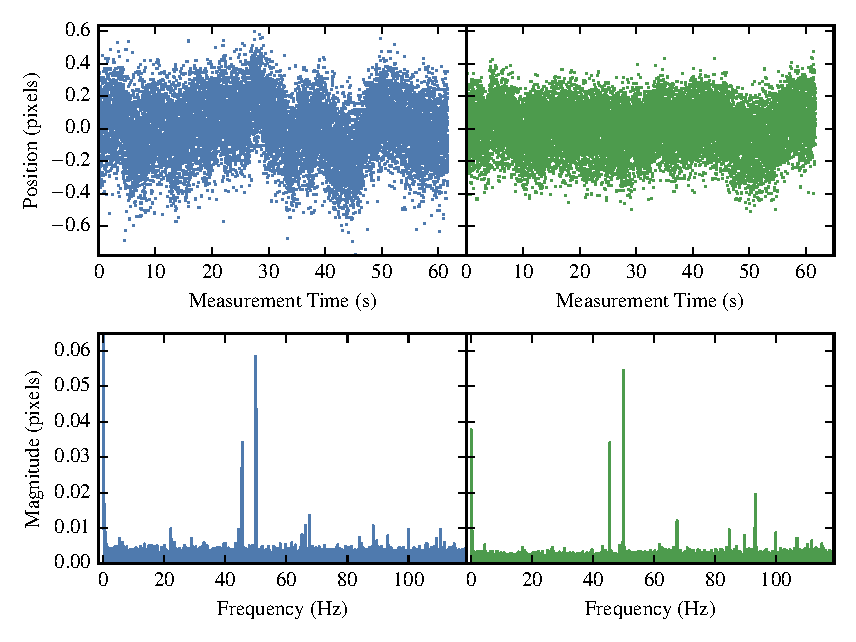
\includegraphics{part2/Figs/cw_beam_stability.pdf}
    \caption{Continuous electron beam.}
    \label{figure:cw_stability}
    \end{subfigure}

    \begin{subfigure}{\linewidth}
    \centering
    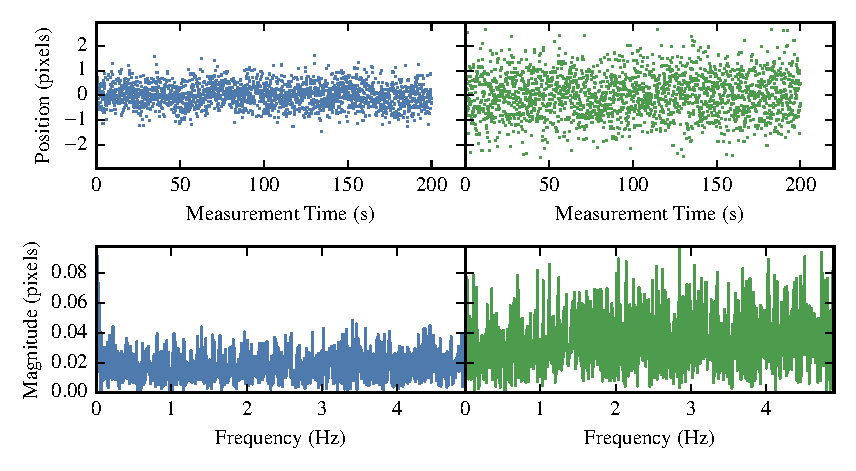
\includegraphics{part2/Figs/pulse_beam_stability.pdf}
    \caption{Pulsed electron beam.}
    \label{figure:pulse_stability}
    \end{subfigure}
    \caption{Beam position and position spectrum for $x$ (blue) and $y$ (green) directions for \gls{cw}-mode electrons (top) and pulse-mode electrons (bottom).
    Pulsed operation is limited to \unit[10]{Hz} and thus the spectrum is limited to \unit[5]{Hz}. The continuous beam spectrum was limited by the camera speed of \unit[240]{Hz}.}
    \label{figure:stability}
\end{figure}

\subsection{Summary}

It was hoped that continuous mode would provide a viable alternative to normal pulsed operation with this iteration of the \gls{caes} with better beam current and stability.
The investigations in this section indicate that, with the current apparatus, continuous mode is on-par or worse than pulsed-mode with respect to beam current and stability.
With significant investments of time and money it would be possible to achieve better current and stability with continuous mode however with the next iteration of the experiment on the near-horizon it is not worth pursuing these avenues with this apparatus.

\section{Registration}\label{section:registration}

Instability in the beam path (see Section~\ref{section:stability}) results in the electron beam drifting around the detector from shot-to-shot.
When multi-shot averages are required the beam drift results in the beam being `smeared' when averaged.
It is necessary to `register' the sets of images to prevent this smearing, see Figure~\ref{figure:registration_examples}.

\begin{figure}
    \center
    %% Creator: Matplotlib, PGF backend
%%
%% To include the figure in your LaTeX document, write
%%   \input{<filename>.pgf}
%%
%% Make sure the required packages are loaded in your preamble
%%   \usepackage{pgf}
%%
%% Figures using additional raster images can only be included by \input if
%% they are in the same directory as the main LaTeX file. For loading figures
%% from other directories you can use the `import` package
%%   \usepackage{import}
%% and then include the figures with
%%   \import{<path to file>}{<filename>.pgf}
%%
%% Matplotlib used the following preamble
%%
\begingroup%
\makeatletter%
\begin{pgfpicture}%
\pgfpathrectangle{\pgfpointorigin}{\pgfqpoint{5.710000in}{5.710000in}}%
\pgfusepath{use as bounding box, clip}%
\begin{pgfscope}%
\pgfsetbuttcap%
\pgfsetmiterjoin%
\definecolor{currentfill}{rgb}{1.000000,1.000000,1.000000}%
\pgfsetfillcolor{currentfill}%
\pgfsetlinewidth{0.000000pt}%
\definecolor{currentstroke}{rgb}{1.000000,1.000000,1.000000}%
\pgfsetstrokecolor{currentstroke}%
\pgfsetdash{}{0pt}%
\pgfpathmoveto{\pgfqpoint{0.000000in}{0.000000in}}%
\pgfpathlineto{\pgfqpoint{5.710000in}{0.000000in}}%
\pgfpathlineto{\pgfqpoint{5.710000in}{5.710000in}}%
\pgfpathlineto{\pgfqpoint{0.000000in}{5.710000in}}%
\pgfpathclose%
\pgfusepath{fill}%
\end{pgfscope}%
\begin{pgfscope}%
\pgfsetbuttcap%
\pgfsetmiterjoin%
\definecolor{currentfill}{rgb}{1.000000,1.000000,1.000000}%
\pgfsetfillcolor{currentfill}%
\pgfsetlinewidth{0.000000pt}%
\definecolor{currentstroke}{rgb}{0.000000,0.000000,0.000000}%
\pgfsetstrokecolor{currentstroke}%
\pgfsetstrokeopacity{0.000000}%
\pgfsetdash{}{0pt}%
\pgfpathmoveto{\pgfqpoint{0.216430in}{2.913778in}}%
\pgfpathlineto{\pgfqpoint{2.713570in}{2.913778in}}%
\pgfpathlineto{\pgfqpoint{2.713570in}{5.410919in}}%
\pgfpathlineto{\pgfqpoint{0.216430in}{5.410919in}}%
\pgfpathclose%
\pgfusepath{fill}%
\end{pgfscope}%
\begin{pgfscope}%
\pgfpathrectangle{\pgfqpoint{0.216430in}{2.913778in}}{\pgfqpoint{2.497141in}{2.497141in}} %
\pgfusepath{clip}%
\pgftext[at=\pgfqpoint{0.216430in}{2.913778in},left,bottom]{\pgfimage[interpolate=true,width=2.500000in,height=2.510000in]{registration_examples-img0.png}}%
\end{pgfscope}%
\begin{pgfscope}%
\pgfsetrectcap%
\pgfsetmiterjoin%
\pgfsetlinewidth{1.003750pt}%
\definecolor{currentstroke}{rgb}{0.000000,0.000000,0.000000}%
\pgfsetstrokecolor{currentstroke}%
\pgfsetdash{}{0pt}%
\pgfpathmoveto{\pgfqpoint{2.713570in}{2.913778in}}%
\pgfpathlineto{\pgfqpoint{2.713570in}{5.410919in}}%
\pgfusepath{stroke}%
\end{pgfscope}%
\begin{pgfscope}%
\pgfsetrectcap%
\pgfsetmiterjoin%
\pgfsetlinewidth{1.003750pt}%
\definecolor{currentstroke}{rgb}{0.000000,0.000000,0.000000}%
\pgfsetstrokecolor{currentstroke}%
\pgfsetdash{}{0pt}%
\pgfpathmoveto{\pgfqpoint{0.216430in}{2.913778in}}%
\pgfpathlineto{\pgfqpoint{2.713570in}{2.913778in}}%
\pgfusepath{stroke}%
\end{pgfscope}%
\begin{pgfscope}%
\pgfsetrectcap%
\pgfsetmiterjoin%
\pgfsetlinewidth{1.003750pt}%
\definecolor{currentstroke}{rgb}{0.000000,0.000000,0.000000}%
\pgfsetstrokecolor{currentstroke}%
\pgfsetdash{}{0pt}%
\pgfpathmoveto{\pgfqpoint{0.216430in}{2.913778in}}%
\pgfpathlineto{\pgfqpoint{0.216430in}{5.410919in}}%
\pgfusepath{stroke}%
\end{pgfscope}%
\begin{pgfscope}%
\pgfsetrectcap%
\pgfsetmiterjoin%
\pgfsetlinewidth{1.003750pt}%
\definecolor{currentstroke}{rgb}{0.000000,0.000000,0.000000}%
\pgfsetstrokecolor{currentstroke}%
\pgfsetdash{}{0pt}%
\pgfpathmoveto{\pgfqpoint{0.216430in}{5.410919in}}%
\pgfpathlineto{\pgfqpoint{2.713570in}{5.410919in}}%
\pgfusepath{stroke}%
\end{pgfscope}%
\begin{pgfscope}%
\pgftext[x=1.465000in,y=5.480364in,,base]{\fontsize{12.000000}{14.400000}\selectfont Single-Shot}%
\end{pgfscope}%
\begin{pgfscope}%
\pgfsetbuttcap%
\pgfsetmiterjoin%
\definecolor{currentfill}{rgb}{1.000000,1.000000,1.000000}%
\pgfsetfillcolor{currentfill}%
\pgfsetlinewidth{0.000000pt}%
\definecolor{currentstroke}{rgb}{0.000000,0.000000,0.000000}%
\pgfsetstrokecolor{currentstroke}%
\pgfsetstrokeopacity{0.000000}%
\pgfsetdash{}{0pt}%
\pgfpathmoveto{\pgfqpoint{2.996430in}{2.913778in}}%
\pgfpathlineto{\pgfqpoint{5.493570in}{2.913778in}}%
\pgfpathlineto{\pgfqpoint{5.493570in}{5.410919in}}%
\pgfpathlineto{\pgfqpoint{2.996430in}{5.410919in}}%
\pgfpathclose%
\pgfusepath{fill}%
\end{pgfscope}%
\begin{pgfscope}%
\pgfpathrectangle{\pgfqpoint{2.996430in}{2.913778in}}{\pgfqpoint{2.497141in}{2.497141in}} %
\pgfusepath{clip}%
\pgftext[at=\pgfqpoint{2.996430in}{2.913778in},left,bottom]{\pgfimage[interpolate=true,width=2.500000in,height=2.510000in]{registration_examples-img1.png}}%
\end{pgfscope}%
\begin{pgfscope}%
\pgfsetrectcap%
\pgfsetmiterjoin%
\pgfsetlinewidth{1.003750pt}%
\definecolor{currentstroke}{rgb}{0.000000,0.000000,0.000000}%
\pgfsetstrokecolor{currentstroke}%
\pgfsetdash{}{0pt}%
\pgfpathmoveto{\pgfqpoint{5.493570in}{2.913778in}}%
\pgfpathlineto{\pgfqpoint{5.493570in}{5.410919in}}%
\pgfusepath{stroke}%
\end{pgfscope}%
\begin{pgfscope}%
\pgfsetrectcap%
\pgfsetmiterjoin%
\pgfsetlinewidth{1.003750pt}%
\definecolor{currentstroke}{rgb}{0.000000,0.000000,0.000000}%
\pgfsetstrokecolor{currentstroke}%
\pgfsetdash{}{0pt}%
\pgfpathmoveto{\pgfqpoint{2.996430in}{2.913778in}}%
\pgfpathlineto{\pgfqpoint{5.493570in}{2.913778in}}%
\pgfusepath{stroke}%
\end{pgfscope}%
\begin{pgfscope}%
\pgfsetrectcap%
\pgfsetmiterjoin%
\pgfsetlinewidth{1.003750pt}%
\definecolor{currentstroke}{rgb}{0.000000,0.000000,0.000000}%
\pgfsetstrokecolor{currentstroke}%
\pgfsetdash{}{0pt}%
\pgfpathmoveto{\pgfqpoint{2.996430in}{2.913778in}}%
\pgfpathlineto{\pgfqpoint{2.996430in}{5.410919in}}%
\pgfusepath{stroke}%
\end{pgfscope}%
\begin{pgfscope}%
\pgfsetrectcap%
\pgfsetmiterjoin%
\pgfsetlinewidth{1.003750pt}%
\definecolor{currentstroke}{rgb}{0.000000,0.000000,0.000000}%
\pgfsetstrokecolor{currentstroke}%
\pgfsetdash{}{0pt}%
\pgfpathmoveto{\pgfqpoint{2.996430in}{5.410919in}}%
\pgfpathlineto{\pgfqpoint{5.493570in}{5.410919in}}%
\pgfusepath{stroke}%
\end{pgfscope}%
\begin{pgfscope}%
\pgftext[x=4.245000in,y=5.480364in,,base]{\fontsize{12.000000}{14.400000}\selectfont Average}%
\end{pgfscope}%
\begin{pgfscope}%
\pgfsetbuttcap%
\pgfsetmiterjoin%
\definecolor{currentfill}{rgb}{1.000000,1.000000,1.000000}%
\pgfsetfillcolor{currentfill}%
\pgfsetlinewidth{0.000000pt}%
\definecolor{currentstroke}{rgb}{0.000000,0.000000,0.000000}%
\pgfsetstrokecolor{currentstroke}%
\pgfsetstrokeopacity{0.000000}%
\pgfsetdash{}{0pt}%
\pgfpathmoveto{\pgfqpoint{0.216430in}{0.150000in}}%
\pgfpathlineto{\pgfqpoint{2.713570in}{0.150000in}}%
\pgfpathlineto{\pgfqpoint{2.713570in}{2.647141in}}%
\pgfpathlineto{\pgfqpoint{0.216430in}{2.647141in}}%
\pgfpathclose%
\pgfusepath{fill}%
\end{pgfscope}%
\begin{pgfscope}%
\pgfpathrectangle{\pgfqpoint{0.216430in}{0.150000in}}{\pgfqpoint{2.497141in}{2.497141in}} %
\pgfusepath{clip}%
\pgftext[at=\pgfqpoint{0.216430in}{0.150000in},left,bottom]{\pgfimage[interpolate=true,width=2.500000in,height=2.510000in]{registration_examples-img2.png}}%
\end{pgfscope}%
\begin{pgfscope}%
\pgfsetrectcap%
\pgfsetmiterjoin%
\pgfsetlinewidth{1.003750pt}%
\definecolor{currentstroke}{rgb}{0.000000,0.000000,0.000000}%
\pgfsetstrokecolor{currentstroke}%
\pgfsetdash{}{0pt}%
\pgfpathmoveto{\pgfqpoint{2.713570in}{0.150000in}}%
\pgfpathlineto{\pgfqpoint{2.713570in}{2.647141in}}%
\pgfusepath{stroke}%
\end{pgfscope}%
\begin{pgfscope}%
\pgfsetrectcap%
\pgfsetmiterjoin%
\pgfsetlinewidth{1.003750pt}%
\definecolor{currentstroke}{rgb}{0.000000,0.000000,0.000000}%
\pgfsetstrokecolor{currentstroke}%
\pgfsetdash{}{0pt}%
\pgfpathmoveto{\pgfqpoint{0.216430in}{0.150000in}}%
\pgfpathlineto{\pgfqpoint{2.713570in}{0.150000in}}%
\pgfusepath{stroke}%
\end{pgfscope}%
\begin{pgfscope}%
\pgfsetrectcap%
\pgfsetmiterjoin%
\pgfsetlinewidth{1.003750pt}%
\definecolor{currentstroke}{rgb}{0.000000,0.000000,0.000000}%
\pgfsetstrokecolor{currentstroke}%
\pgfsetdash{}{0pt}%
\pgfpathmoveto{\pgfqpoint{0.216430in}{0.150000in}}%
\pgfpathlineto{\pgfqpoint{0.216430in}{2.647141in}}%
\pgfusepath{stroke}%
\end{pgfscope}%
\begin{pgfscope}%
\pgfsetrectcap%
\pgfsetmiterjoin%
\pgfsetlinewidth{1.003750pt}%
\definecolor{currentstroke}{rgb}{0.000000,0.000000,0.000000}%
\pgfsetstrokecolor{currentstroke}%
\pgfsetdash{}{0pt}%
\pgfpathmoveto{\pgfqpoint{0.216430in}{2.647141in}}%
\pgfpathlineto{\pgfqpoint{2.713570in}{2.647141in}}%
\pgfusepath{stroke}%
\end{pgfscope}%
\begin{pgfscope}%
\pgftext[x=1.465000in,y=2.716585in,,base]{\fontsize{12.000000}{14.400000}\selectfont Slipped}%
\end{pgfscope}%
\begin{pgfscope}%
\pgfsetbuttcap%
\pgfsetmiterjoin%
\definecolor{currentfill}{rgb}{1.000000,1.000000,1.000000}%
\pgfsetfillcolor{currentfill}%
\pgfsetlinewidth{0.000000pt}%
\definecolor{currentstroke}{rgb}{0.000000,0.000000,0.000000}%
\pgfsetstrokecolor{currentstroke}%
\pgfsetstrokeopacity{0.000000}%
\pgfsetdash{}{0pt}%
\pgfpathmoveto{\pgfqpoint{2.996430in}{0.150000in}}%
\pgfpathlineto{\pgfqpoint{5.493570in}{0.150000in}}%
\pgfpathlineto{\pgfqpoint{5.493570in}{2.647141in}}%
\pgfpathlineto{\pgfqpoint{2.996430in}{2.647141in}}%
\pgfpathclose%
\pgfusepath{fill}%
\end{pgfscope}%
\begin{pgfscope}%
\pgfpathrectangle{\pgfqpoint{2.996430in}{0.150000in}}{\pgfqpoint{2.497141in}{2.497141in}} %
\pgfusepath{clip}%
\pgftext[at=\pgfqpoint{2.996430in}{0.150000in},left,bottom]{\pgfimage[interpolate=true,width=2.500000in,height=2.510000in]{registration_examples-img3.png}}%
\end{pgfscope}%
\begin{pgfscope}%
\pgfsetrectcap%
\pgfsetmiterjoin%
\pgfsetlinewidth{1.003750pt}%
\definecolor{currentstroke}{rgb}{0.000000,0.000000,0.000000}%
\pgfsetstrokecolor{currentstroke}%
\pgfsetdash{}{0pt}%
\pgfpathmoveto{\pgfqpoint{5.493570in}{0.150000in}}%
\pgfpathlineto{\pgfqpoint{5.493570in}{2.647141in}}%
\pgfusepath{stroke}%
\end{pgfscope}%
\begin{pgfscope}%
\pgfsetrectcap%
\pgfsetmiterjoin%
\pgfsetlinewidth{1.003750pt}%
\definecolor{currentstroke}{rgb}{0.000000,0.000000,0.000000}%
\pgfsetstrokecolor{currentstroke}%
\pgfsetdash{}{0pt}%
\pgfpathmoveto{\pgfqpoint{2.996430in}{0.150000in}}%
\pgfpathlineto{\pgfqpoint{5.493570in}{0.150000in}}%
\pgfusepath{stroke}%
\end{pgfscope}%
\begin{pgfscope}%
\pgfsetrectcap%
\pgfsetmiterjoin%
\pgfsetlinewidth{1.003750pt}%
\definecolor{currentstroke}{rgb}{0.000000,0.000000,0.000000}%
\pgfsetstrokecolor{currentstroke}%
\pgfsetdash{}{0pt}%
\pgfpathmoveto{\pgfqpoint{2.996430in}{0.150000in}}%
\pgfpathlineto{\pgfqpoint{2.996430in}{2.647141in}}%
\pgfusepath{stroke}%
\end{pgfscope}%
\begin{pgfscope}%
\pgfsetrectcap%
\pgfsetmiterjoin%
\pgfsetlinewidth{1.003750pt}%
\definecolor{currentstroke}{rgb}{0.000000,0.000000,0.000000}%
\pgfsetstrokecolor{currentstroke}%
\pgfsetdash{}{0pt}%
\pgfpathmoveto{\pgfqpoint{2.996430in}{2.647141in}}%
\pgfpathlineto{\pgfqpoint{5.493570in}{2.647141in}}%
\pgfusepath{stroke}%
\end{pgfscope}%
\begin{pgfscope}%
\pgftext[x=4.245000in,y=2.716585in,,base]{\fontsize{12.000000}{14.400000}\selectfont Registered}%
\end{pgfscope}%
\end{pgfpicture}%
\makeatother%
\endgroup%

    \caption{Single-Shot is a single image from a streaked pepperpot data set of 1000 images. Average is the simple average of all 1000 images. Slipped is an attempt at registration that only looks for the maximum value of the convolution with no limit on shot-to-shot variation, there is an additional, faint beamlet visible at the top of the image. Registration is a successful registration where a shot-to-shot limit to drift of 5 pixels was enforced. Below each image is the row sum of the image. All the images are independently log scaled.}
    \label{figure:registration_examples}
    % Data and code in 2017.07.24 plot_registration_examples.py
\end{figure}

Registration consisted of convolving each image with a reference image, recording the location of the maximum value of the convolution and then using that location to align all the images.
The reference image usually consists of either just the first image in the set or the average image of the entire set, depending on the amount of signal in a single image.
The registration process can also be performed iteratively where the reference image becomes the aligned output of the previous iteration.

Registration functions very well for high signal, structured data such as diffraction patterns (see Chapter~\ref{chapter:diffraction}) or pepperpot beam masks (see Chapter~\ref{chapter:brightness}).
Low signal data can be registered as long there is enough signal in a single shot for the convolution to correctly identify the features in the image.
Unstructured data or continuous data, such as large flat beam profiles, will not register well as the convolution with not be able to identify common features well.

Lower signal data requires more care than high signal data and in some cases cannot be registered.
One of the registration errors that has occurred with pepperpot data is `slipping' where the convolution maxima correspond to neighbouring beamlets rather than the same beamlet and thus the images are incorrectly aligned.
This error can be evaded by applying a limit to how far the convolution maxima of an image can change from shot to shot, generally the limit should be less than the distance between beamlets.
This allows slow drift of the beam path to be dealt with while preventing slipping.

Slipped, and therefore failed, pepperpot registrations were usually easy to identify since the number of beamlets was known and slipped errors results in extra beamlets appearing in the the registered image.
While registering the pepperpots the best results were provided with around 3 iterations and limits on the shot-to-shot drift less than distance between the pepperpots.
An example of a slipped registration is shown in Figure~\ref{figure:registration_examples} using data from Chapter~\ref{chapter:brightness}.

{\color{red} I'm still not happy with this example of slipping. I should look for a better one. I may have to engineer one.}

\section{Astigmatism}\label{section:quadrupole}

During the investigations already discussed in this section beam astigmatism was observed in the electron beam.
The astigmatism was apparent when the strength of the electron lenses were adjusted or while translating the \gls{mcp} detector past a beam focus as the two orthogonal transverse axes did not share a focus, as shown in Figures~\ref{figure:astigmatism_translation} and \ref{figure:quadrupole_scans_off}.
While varying the strength of the Einzel lens the electron beam can be seen to pass through two foci as shown in Figures~\ref{figure:quadrupole_scans_off}.

\begin{figure}
    \centering
    %% Creator: Matplotlib, PGF backend
%%
%% To include the figure in your LaTeX document, write
%%   \input{<filename>.pgf}
%%
%% Make sure the required packages are loaded in your preamble
%%   \usepackage{pgf}
%%
%% Figures using additional raster images can only be included by \input if
%% they are in the same directory as the main LaTeX file. For loading figures
%% from other directories you can use the `import` package
%%   \usepackage{import}
%% and then include the figures with
%%   \import{<path to file>}{<filename>.pgf}
%%
%% Matplotlib used the following preamble
%%
\begingroup%
\makeatletter%
\begin{pgfpicture}%
\pgfpathrectangle{\pgfpointorigin}{\pgfqpoint{4.282500in}{2.855000in}}%
\pgfusepath{use as bounding box, clip}%
\begin{pgfscope}%
\pgfsetbuttcap%
\pgfsetmiterjoin%
\definecolor{currentfill}{rgb}{1.000000,1.000000,1.000000}%
\pgfsetfillcolor{currentfill}%
\pgfsetlinewidth{0.000000pt}%
\definecolor{currentstroke}{rgb}{1.000000,1.000000,1.000000}%
\pgfsetstrokecolor{currentstroke}%
\pgfsetdash{}{0pt}%
\pgfpathmoveto{\pgfqpoint{0.000000in}{0.000000in}}%
\pgfpathlineto{\pgfqpoint{4.282500in}{0.000000in}}%
\pgfpathlineto{\pgfqpoint{4.282500in}{2.855000in}}%
\pgfpathlineto{\pgfqpoint{0.000000in}{2.855000in}}%
\pgfpathclose%
\pgfusepath{fill}%
\end{pgfscope}%
\begin{pgfscope}%
\pgfsetbuttcap%
\pgfsetmiterjoin%
\definecolor{currentfill}{rgb}{1.000000,1.000000,1.000000}%
\pgfsetfillcolor{currentfill}%
\pgfsetlinewidth{0.000000pt}%
\definecolor{currentstroke}{rgb}{0.000000,0.000000,0.000000}%
\pgfsetstrokecolor{currentstroke}%
\pgfsetstrokeopacity{0.000000}%
\pgfsetdash{}{0pt}%
\pgfpathmoveto{\pgfqpoint{0.571250in}{0.521575in}}%
\pgfpathlineto{\pgfqpoint{4.132500in}{0.521575in}}%
\pgfpathlineto{\pgfqpoint{4.132500in}{2.643356in}}%
\pgfpathlineto{\pgfqpoint{0.571250in}{2.643356in}}%
\pgfpathclose%
\pgfusepath{fill}%
\end{pgfscope}%
\begin{pgfscope}%
\pgfpathrectangle{\pgfqpoint{0.571250in}{0.521575in}}{\pgfqpoint{3.561250in}{2.121782in}} %
\pgfusepath{clip}%
\pgfsetbuttcap%
\pgfsetroundjoin%
\definecolor{currentfill}{rgb}{0.000000,0.000000,1.000000}%
\pgfsetfillcolor{currentfill}%
\pgfsetlinewidth{0.501875pt}%
\definecolor{currentstroke}{rgb}{0.000000,0.000000,1.000000}%
\pgfsetstrokecolor{currentstroke}%
\pgfsetdash{}{0pt}%
\pgfsys@defobject{currentmarker}{\pgfqpoint{-0.041667in}{-0.041667in}}{\pgfqpoint{0.041667in}{0.041667in}}{%
\pgfpathmoveto{\pgfqpoint{-0.041667in}{-0.041667in}}%
\pgfpathlineto{\pgfqpoint{0.041667in}{0.041667in}}%
\pgfpathmoveto{\pgfqpoint{-0.041667in}{0.041667in}}%
\pgfpathlineto{\pgfqpoint{0.041667in}{-0.041667in}}%
\pgfusepath{stroke,fill}%
}%
\begin{pgfscope}%
\pgfsys@transformshift{3.117880in}{1.380816in}%
\pgfsys@useobject{currentmarker}{}%
\end{pgfscope}%
\begin{pgfscope}%
\pgfsys@transformshift{3.789814in}{1.302657in}%
\pgfsys@useobject{currentmarker}{}%
\end{pgfscope}%
\begin{pgfscope}%
\pgfsys@transformshift{0.766111in}{2.349479in}%
\pgfsys@useobject{currentmarker}{}%
\end{pgfscope}%
\begin{pgfscope}%
\pgfsys@transformshift{1.774012in}{1.757995in}%
\pgfsys@useobject{currentmarker}{}%
\end{pgfscope}%
\begin{pgfscope}%
\pgfsys@transformshift{2.445946in}{1.557808in}%
\pgfsys@useobject{currentmarker}{}%
\end{pgfscope}%
\begin{pgfscope}%
\pgfsys@transformshift{1.102078in}{2.202239in}%
\pgfsys@useobject{currentmarker}{}%
\end{pgfscope}%
\begin{pgfscope}%
\pgfsys@transformshift{2.781913in}{1.409558in}%
\pgfsys@useobject{currentmarker}{}%
\end{pgfscope}%
\begin{pgfscope}%
\pgfsys@transformshift{2.109979in}{1.646555in}%
\pgfsys@useobject{currentmarker}{}%
\end{pgfscope}%
\begin{pgfscope}%
\pgfsys@transformshift{3.453847in}{1.288034in}%
\pgfsys@useobject{currentmarker}{}%
\end{pgfscope}%
\begin{pgfscope}%
\pgfsys@transformshift{1.438045in}{1.904731in}%
\pgfsys@useobject{currentmarker}{}%
\end{pgfscope}%
\begin{pgfscope}%
\pgfsys@transformshift{3.991394in}{1.360142in}%
\pgfsys@useobject{currentmarker}{}%
\end{pgfscope}%
\end{pgfscope}%
\begin{pgfscope}%
\pgfpathrectangle{\pgfqpoint{0.571250in}{0.521575in}}{\pgfqpoint{3.561250in}{2.121782in}} %
\pgfusepath{clip}%
\pgfsetbuttcap%
\pgfsetroundjoin%
\definecolor{currentfill}{rgb}{0.000000,0.500000,0.000000}%
\pgfsetfillcolor{currentfill}%
\pgfsetlinewidth{0.501875pt}%
\definecolor{currentstroke}{rgb}{0.000000,0.500000,0.000000}%
\pgfsetstrokecolor{currentstroke}%
\pgfsetdash{}{0pt}%
\pgfsys@defobject{currentmarker}{\pgfqpoint{-0.041667in}{-0.041667in}}{\pgfqpoint{0.041667in}{0.041667in}}{%
\pgfpathmoveto{\pgfqpoint{-0.041667in}{-0.041667in}}%
\pgfpathlineto{\pgfqpoint{0.041667in}{0.041667in}}%
\pgfpathmoveto{\pgfqpoint{-0.041667in}{0.041667in}}%
\pgfpathlineto{\pgfqpoint{0.041667in}{-0.041667in}}%
\pgfusepath{stroke,fill}%
}%
\begin{pgfscope}%
\pgfsys@transformshift{3.117880in}{1.602686in}%
\pgfsys@useobject{currentmarker}{}%
\end{pgfscope}%
\begin{pgfscope}%
\pgfsys@transformshift{3.789814in}{2.161394in}%
\pgfsys@useobject{currentmarker}{}%
\end{pgfscope}%
\begin{pgfscope}%
\pgfsys@transformshift{0.766111in}{1.244669in}%
\pgfsys@useobject{currentmarker}{}%
\end{pgfscope}%
\begin{pgfscope}%
\pgfsys@transformshift{1.774012in}{1.352578in}%
\pgfsys@useobject{currentmarker}{}%
\end{pgfscope}%
\begin{pgfscope}%
\pgfsys@transformshift{2.445946in}{1.469564in}%
\pgfsys@useobject{currentmarker}{}%
\end{pgfscope}%
\begin{pgfscope}%
\pgfsys@transformshift{1.102078in}{1.322827in}%
\pgfsys@useobject{currentmarker}{}%
\end{pgfscope}%
\begin{pgfscope}%
\pgfsys@transformshift{2.781913in}{1.520997in}%
\pgfsys@useobject{currentmarker}{}%
\end{pgfscope}%
\begin{pgfscope}%
\pgfsys@transformshift{2.109979in}{1.432249in}%
\pgfsys@useobject{currentmarker}{}%
\end{pgfscope}%
\begin{pgfscope}%
\pgfsys@transformshift{3.453847in}{1.854306in}%
\pgfsys@useobject{currentmarker}{}%
\end{pgfscope}%
\begin{pgfscope}%
\pgfsys@transformshift{1.438045in}{1.399977in}%
\pgfsys@useobject{currentmarker}{}%
\end{pgfscope}%
\begin{pgfscope}%
\pgfsys@transformshift{3.991394in}{2.278380in}%
\pgfsys@useobject{currentmarker}{}%
\end{pgfscope}%
\end{pgfscope}%
\begin{pgfscope}%
\pgfpathrectangle{\pgfqpoint{0.571250in}{0.521575in}}{\pgfqpoint{3.561250in}{2.121782in}} %
\pgfusepath{clip}%
\pgfsetrectcap%
\pgfsetroundjoin%
\pgfsetlinewidth{1.003750pt}%
\definecolor{currentstroke}{rgb}{0.309804,0.478431,0.682353}%
\pgfsetstrokecolor{currentstroke}%
\pgfsetdash{}{0pt}%
\pgfpathmoveto{\pgfqpoint{0.561250in}{2.435770in}}%
\pgfpathlineto{\pgfqpoint{0.828838in}{2.291395in}}%
\pgfpathlineto{\pgfqpoint{1.073156in}{2.162018in}}%
\pgfpathlineto{\pgfqpoint{1.290327in}{2.049469in}}%
\pgfpathlineto{\pgfqpoint{1.487138in}{1.949942in}}%
\pgfpathlineto{\pgfqpoint{1.663590in}{1.863153in}}%
\pgfpathlineto{\pgfqpoint{1.826468in}{1.785518in}}%
\pgfpathlineto{\pgfqpoint{1.975773in}{1.716850in}}%
\pgfpathlineto{\pgfqpoint{2.111505in}{1.656874in}}%
\pgfpathlineto{\pgfqpoint{2.233664in}{1.605222in}}%
\pgfpathlineto{\pgfqpoint{2.349037in}{1.558772in}}%
\pgfpathlineto{\pgfqpoint{2.457622in}{1.517414in}}%
\pgfpathlineto{\pgfqpoint{2.559421in}{1.480989in}}%
\pgfpathlineto{\pgfqpoint{2.654434in}{1.449283in}}%
\pgfpathlineto{\pgfqpoint{2.742659in}{1.422034in}}%
\pgfpathlineto{\pgfqpoint{2.830885in}{1.397096in}}%
\pgfpathlineto{\pgfqpoint{2.912324in}{1.376305in}}%
\pgfpathlineto{\pgfqpoint{2.993764in}{1.357816in}}%
\pgfpathlineto{\pgfqpoint{3.068416in}{1.343024in}}%
\pgfpathlineto{\pgfqpoint{3.143069in}{1.330412in}}%
\pgfpathlineto{\pgfqpoint{3.217721in}{1.320082in}}%
\pgfpathlineto{\pgfqpoint{3.292374in}{1.312125in}}%
\pgfpathlineto{\pgfqpoint{3.360240in}{1.307010in}}%
\pgfpathlineto{\pgfqpoint{3.428106in}{1.303955in}}%
\pgfpathlineto{\pgfqpoint{3.495972in}{1.302985in}}%
\pgfpathlineto{\pgfqpoint{3.563838in}{1.304106in}}%
\pgfpathlineto{\pgfqpoint{3.631704in}{1.307310in}}%
\pgfpathlineto{\pgfqpoint{3.699570in}{1.312571in}}%
\pgfpathlineto{\pgfqpoint{3.774223in}{1.320687in}}%
\pgfpathlineto{\pgfqpoint{3.848875in}{1.331169in}}%
\pgfpathlineto{\pgfqpoint{3.923528in}{1.343927in}}%
\pgfpathlineto{\pgfqpoint{3.991394in}{1.357413in}}%
\pgfpathlineto{\pgfqpoint{3.991394in}{1.357413in}}%
\pgfusepath{stroke}%
\end{pgfscope}%
\begin{pgfscope}%
\pgfpathrectangle{\pgfqpoint{0.571250in}{0.521575in}}{\pgfqpoint{3.561250in}{2.121782in}} %
\pgfusepath{clip}%
\pgfsetrectcap%
\pgfsetroundjoin%
\pgfsetlinewidth{1.003750pt}%
\definecolor{currentstroke}{rgb}{0.301961,0.607843,0.301961}%
\pgfsetstrokecolor{currentstroke}%
\pgfsetdash{}{0pt}%
\pgfpathmoveto{\pgfqpoint{0.561250in}{1.413087in}}%
\pgfpathlineto{\pgfqpoint{0.652386in}{1.387460in}}%
\pgfpathlineto{\pgfqpoint{0.740612in}{1.364888in}}%
\pgfpathlineto{\pgfqpoint{0.828838in}{1.344696in}}%
\pgfpathlineto{\pgfqpoint{0.910277in}{1.328325in}}%
\pgfpathlineto{\pgfqpoint{0.991716in}{1.314271in}}%
\pgfpathlineto{\pgfqpoint{1.066369in}{1.303531in}}%
\pgfpathlineto{\pgfqpoint{1.141022in}{1.294928in}}%
\pgfpathlineto{\pgfqpoint{1.215674in}{1.288533in}}%
\pgfpathlineto{\pgfqpoint{1.290327in}{1.284404in}}%
\pgfpathlineto{\pgfqpoint{1.364979in}{1.282576in}}%
\pgfpathlineto{\pgfqpoint{1.439632in}{1.283067in}}%
\pgfpathlineto{\pgfqpoint{1.514285in}{1.285871in}}%
\pgfpathlineto{\pgfqpoint{1.588937in}{1.290964in}}%
\pgfpathlineto{\pgfqpoint{1.663590in}{1.298300in}}%
\pgfpathlineto{\pgfqpoint{1.738242in}{1.307817in}}%
\pgfpathlineto{\pgfqpoint{1.812895in}{1.319437in}}%
\pgfpathlineto{\pgfqpoint{1.894334in}{1.334404in}}%
\pgfpathlineto{\pgfqpoint{1.975773in}{1.351637in}}%
\pgfpathlineto{\pgfqpoint{2.063999in}{1.372701in}}%
\pgfpathlineto{\pgfqpoint{2.152225in}{1.396082in}}%
\pgfpathlineto{\pgfqpoint{2.247237in}{1.423645in}}%
\pgfpathlineto{\pgfqpoint{2.342250in}{1.453465in}}%
\pgfpathlineto{\pgfqpoint{2.444049in}{1.487681in}}%
\pgfpathlineto{\pgfqpoint{2.552635in}{1.526500in}}%
\pgfpathlineto{\pgfqpoint{2.668007in}{1.570076in}}%
\pgfpathlineto{\pgfqpoint{2.790166in}{1.618523in}}%
\pgfpathlineto{\pgfqpoint{2.925898in}{1.674777in}}%
\pgfpathlineto{\pgfqpoint{3.075203in}{1.739195in}}%
\pgfpathlineto{\pgfqpoint{3.231295in}{1.808964in}}%
\pgfpathlineto{\pgfqpoint{3.407746in}{1.890345in}}%
\pgfpathlineto{\pgfqpoint{3.597771in}{1.980475in}}%
\pgfpathlineto{\pgfqpoint{3.808156in}{2.082743in}}%
\pgfpathlineto{\pgfqpoint{3.991394in}{2.173575in}}%
\pgfpathlineto{\pgfqpoint{3.991394in}{2.173575in}}%
\pgfusepath{stroke}%
\end{pgfscope}%
\begin{pgfscope}%
\pgfsetrectcap%
\pgfsetmiterjoin%
\pgfsetlinewidth{1.003750pt}%
\definecolor{currentstroke}{rgb}{0.000000,0.000000,0.000000}%
\pgfsetstrokecolor{currentstroke}%
\pgfsetdash{}{0pt}%
\pgfpathmoveto{\pgfqpoint{0.571250in}{0.521575in}}%
\pgfpathlineto{\pgfqpoint{4.132500in}{0.521575in}}%
\pgfusepath{stroke}%
\end{pgfscope}%
\begin{pgfscope}%
\pgfsetrectcap%
\pgfsetmiterjoin%
\pgfsetlinewidth{1.003750pt}%
\definecolor{currentstroke}{rgb}{0.000000,0.000000,0.000000}%
\pgfsetstrokecolor{currentstroke}%
\pgfsetdash{}{0pt}%
\pgfpathmoveto{\pgfqpoint{0.571250in}{2.643356in}}%
\pgfpathlineto{\pgfqpoint{4.132500in}{2.643356in}}%
\pgfusepath{stroke}%
\end{pgfscope}%
\begin{pgfscope}%
\pgfsetrectcap%
\pgfsetmiterjoin%
\pgfsetlinewidth{1.003750pt}%
\definecolor{currentstroke}{rgb}{0.000000,0.000000,0.000000}%
\pgfsetstrokecolor{currentstroke}%
\pgfsetdash{}{0pt}%
\pgfpathmoveto{\pgfqpoint{4.132500in}{0.521575in}}%
\pgfpathlineto{\pgfqpoint{4.132500in}{2.643356in}}%
\pgfusepath{stroke}%
\end{pgfscope}%
\begin{pgfscope}%
\pgfsetrectcap%
\pgfsetmiterjoin%
\pgfsetlinewidth{1.003750pt}%
\definecolor{currentstroke}{rgb}{0.000000,0.000000,0.000000}%
\pgfsetstrokecolor{currentstroke}%
\pgfsetdash{}{0pt}%
\pgfpathmoveto{\pgfqpoint{0.571250in}{0.521575in}}%
\pgfpathlineto{\pgfqpoint{0.571250in}{2.643356in}}%
\pgfusepath{stroke}%
\end{pgfscope}%
\begin{pgfscope}%
\pgfsetbuttcap%
\pgfsetroundjoin%
\definecolor{currentfill}{rgb}{0.000000,0.000000,0.000000}%
\pgfsetfillcolor{currentfill}%
\pgfsetlinewidth{0.501875pt}%
\definecolor{currentstroke}{rgb}{0.000000,0.000000,0.000000}%
\pgfsetstrokecolor{currentstroke}%
\pgfsetdash{}{0pt}%
\pgfsys@defobject{currentmarker}{\pgfqpoint{0.000000in}{0.000000in}}{\pgfqpoint{0.000000in}{0.055556in}}{%
\pgfpathmoveto{\pgfqpoint{0.000000in}{0.000000in}}%
\pgfpathlineto{\pgfqpoint{0.000000in}{0.055556in}}%
\pgfusepath{stroke,fill}%
}%
\begin{pgfscope}%
\pgfsys@transformshift{0.571250in}{0.521575in}%
\pgfsys@useobject{currentmarker}{}%
\end{pgfscope}%
\end{pgfscope}%
\begin{pgfscope}%
\pgfsetbuttcap%
\pgfsetroundjoin%
\definecolor{currentfill}{rgb}{0.000000,0.000000,0.000000}%
\pgfsetfillcolor{currentfill}%
\pgfsetlinewidth{0.501875pt}%
\definecolor{currentstroke}{rgb}{0.000000,0.000000,0.000000}%
\pgfsetstrokecolor{currentstroke}%
\pgfsetdash{}{0pt}%
\pgfsys@defobject{currentmarker}{\pgfqpoint{0.000000in}{-0.055556in}}{\pgfqpoint{0.000000in}{0.000000in}}{%
\pgfpathmoveto{\pgfqpoint{0.000000in}{0.000000in}}%
\pgfpathlineto{\pgfqpoint{0.000000in}{-0.055556in}}%
\pgfusepath{stroke,fill}%
}%
\begin{pgfscope}%
\pgfsys@transformshift{0.571250in}{2.643356in}%
\pgfsys@useobject{currentmarker}{}%
\end{pgfscope}%
\end{pgfscope}%
\begin{pgfscope}%
\pgftext[x=0.571250in,y=0.466019in,,top]{\fontsize{10.000000}{12.000000}\selectfont \(\displaystyle 0\)}%
\end{pgfscope}%
\begin{pgfscope}%
\pgfsetbuttcap%
\pgfsetroundjoin%
\definecolor{currentfill}{rgb}{0.000000,0.000000,0.000000}%
\pgfsetfillcolor{currentfill}%
\pgfsetlinewidth{0.501875pt}%
\definecolor{currentstroke}{rgb}{0.000000,0.000000,0.000000}%
\pgfsetstrokecolor{currentstroke}%
\pgfsetdash{}{0pt}%
\pgfsys@defobject{currentmarker}{\pgfqpoint{0.000000in}{0.000000in}}{\pgfqpoint{0.000000in}{0.055556in}}{%
\pgfpathmoveto{\pgfqpoint{0.000000in}{0.000000in}}%
\pgfpathlineto{\pgfqpoint{0.000000in}{0.055556in}}%
\pgfusepath{stroke,fill}%
}%
\begin{pgfscope}%
\pgfsys@transformshift{1.243184in}{0.521575in}%
\pgfsys@useobject{currentmarker}{}%
\end{pgfscope}%
\end{pgfscope}%
\begin{pgfscope}%
\pgfsetbuttcap%
\pgfsetroundjoin%
\definecolor{currentfill}{rgb}{0.000000,0.000000,0.000000}%
\pgfsetfillcolor{currentfill}%
\pgfsetlinewidth{0.501875pt}%
\definecolor{currentstroke}{rgb}{0.000000,0.000000,0.000000}%
\pgfsetstrokecolor{currentstroke}%
\pgfsetdash{}{0pt}%
\pgfsys@defobject{currentmarker}{\pgfqpoint{0.000000in}{-0.055556in}}{\pgfqpoint{0.000000in}{0.000000in}}{%
\pgfpathmoveto{\pgfqpoint{0.000000in}{0.000000in}}%
\pgfpathlineto{\pgfqpoint{0.000000in}{-0.055556in}}%
\pgfusepath{stroke,fill}%
}%
\begin{pgfscope}%
\pgfsys@transformshift{1.243184in}{2.643356in}%
\pgfsys@useobject{currentmarker}{}%
\end{pgfscope}%
\end{pgfscope}%
\begin{pgfscope}%
\pgftext[x=1.243184in,y=0.466019in,,top]{\fontsize{10.000000}{12.000000}\selectfont \(\displaystyle 100\)}%
\end{pgfscope}%
\begin{pgfscope}%
\pgfsetbuttcap%
\pgfsetroundjoin%
\definecolor{currentfill}{rgb}{0.000000,0.000000,0.000000}%
\pgfsetfillcolor{currentfill}%
\pgfsetlinewidth{0.501875pt}%
\definecolor{currentstroke}{rgb}{0.000000,0.000000,0.000000}%
\pgfsetstrokecolor{currentstroke}%
\pgfsetdash{}{0pt}%
\pgfsys@defobject{currentmarker}{\pgfqpoint{0.000000in}{0.000000in}}{\pgfqpoint{0.000000in}{0.055556in}}{%
\pgfpathmoveto{\pgfqpoint{0.000000in}{0.000000in}}%
\pgfpathlineto{\pgfqpoint{0.000000in}{0.055556in}}%
\pgfusepath{stroke,fill}%
}%
\begin{pgfscope}%
\pgfsys@transformshift{1.915118in}{0.521575in}%
\pgfsys@useobject{currentmarker}{}%
\end{pgfscope}%
\end{pgfscope}%
\begin{pgfscope}%
\pgfsetbuttcap%
\pgfsetroundjoin%
\definecolor{currentfill}{rgb}{0.000000,0.000000,0.000000}%
\pgfsetfillcolor{currentfill}%
\pgfsetlinewidth{0.501875pt}%
\definecolor{currentstroke}{rgb}{0.000000,0.000000,0.000000}%
\pgfsetstrokecolor{currentstroke}%
\pgfsetdash{}{0pt}%
\pgfsys@defobject{currentmarker}{\pgfqpoint{0.000000in}{-0.055556in}}{\pgfqpoint{0.000000in}{0.000000in}}{%
\pgfpathmoveto{\pgfqpoint{0.000000in}{0.000000in}}%
\pgfpathlineto{\pgfqpoint{0.000000in}{-0.055556in}}%
\pgfusepath{stroke,fill}%
}%
\begin{pgfscope}%
\pgfsys@transformshift{1.915118in}{2.643356in}%
\pgfsys@useobject{currentmarker}{}%
\end{pgfscope}%
\end{pgfscope}%
\begin{pgfscope}%
\pgftext[x=1.915118in,y=0.466019in,,top]{\fontsize{10.000000}{12.000000}\selectfont \(\displaystyle 200\)}%
\end{pgfscope}%
\begin{pgfscope}%
\pgfsetbuttcap%
\pgfsetroundjoin%
\definecolor{currentfill}{rgb}{0.000000,0.000000,0.000000}%
\pgfsetfillcolor{currentfill}%
\pgfsetlinewidth{0.501875pt}%
\definecolor{currentstroke}{rgb}{0.000000,0.000000,0.000000}%
\pgfsetstrokecolor{currentstroke}%
\pgfsetdash{}{0pt}%
\pgfsys@defobject{currentmarker}{\pgfqpoint{0.000000in}{0.000000in}}{\pgfqpoint{0.000000in}{0.055556in}}{%
\pgfpathmoveto{\pgfqpoint{0.000000in}{0.000000in}}%
\pgfpathlineto{\pgfqpoint{0.000000in}{0.055556in}}%
\pgfusepath{stroke,fill}%
}%
\begin{pgfscope}%
\pgfsys@transformshift{2.587052in}{0.521575in}%
\pgfsys@useobject{currentmarker}{}%
\end{pgfscope}%
\end{pgfscope}%
\begin{pgfscope}%
\pgfsetbuttcap%
\pgfsetroundjoin%
\definecolor{currentfill}{rgb}{0.000000,0.000000,0.000000}%
\pgfsetfillcolor{currentfill}%
\pgfsetlinewidth{0.501875pt}%
\definecolor{currentstroke}{rgb}{0.000000,0.000000,0.000000}%
\pgfsetstrokecolor{currentstroke}%
\pgfsetdash{}{0pt}%
\pgfsys@defobject{currentmarker}{\pgfqpoint{0.000000in}{-0.055556in}}{\pgfqpoint{0.000000in}{0.000000in}}{%
\pgfpathmoveto{\pgfqpoint{0.000000in}{0.000000in}}%
\pgfpathlineto{\pgfqpoint{0.000000in}{-0.055556in}}%
\pgfusepath{stroke,fill}%
}%
\begin{pgfscope}%
\pgfsys@transformshift{2.587052in}{2.643356in}%
\pgfsys@useobject{currentmarker}{}%
\end{pgfscope}%
\end{pgfscope}%
\begin{pgfscope}%
\pgftext[x=2.587052in,y=0.466019in,,top]{\fontsize{10.000000}{12.000000}\selectfont \(\displaystyle 300\)}%
\end{pgfscope}%
\begin{pgfscope}%
\pgfsetbuttcap%
\pgfsetroundjoin%
\definecolor{currentfill}{rgb}{0.000000,0.000000,0.000000}%
\pgfsetfillcolor{currentfill}%
\pgfsetlinewidth{0.501875pt}%
\definecolor{currentstroke}{rgb}{0.000000,0.000000,0.000000}%
\pgfsetstrokecolor{currentstroke}%
\pgfsetdash{}{0pt}%
\pgfsys@defobject{currentmarker}{\pgfqpoint{0.000000in}{0.000000in}}{\pgfqpoint{0.000000in}{0.055556in}}{%
\pgfpathmoveto{\pgfqpoint{0.000000in}{0.000000in}}%
\pgfpathlineto{\pgfqpoint{0.000000in}{0.055556in}}%
\pgfusepath{stroke,fill}%
}%
\begin{pgfscope}%
\pgfsys@transformshift{3.258986in}{0.521575in}%
\pgfsys@useobject{currentmarker}{}%
\end{pgfscope}%
\end{pgfscope}%
\begin{pgfscope}%
\pgfsetbuttcap%
\pgfsetroundjoin%
\definecolor{currentfill}{rgb}{0.000000,0.000000,0.000000}%
\pgfsetfillcolor{currentfill}%
\pgfsetlinewidth{0.501875pt}%
\definecolor{currentstroke}{rgb}{0.000000,0.000000,0.000000}%
\pgfsetstrokecolor{currentstroke}%
\pgfsetdash{}{0pt}%
\pgfsys@defobject{currentmarker}{\pgfqpoint{0.000000in}{-0.055556in}}{\pgfqpoint{0.000000in}{0.000000in}}{%
\pgfpathmoveto{\pgfqpoint{0.000000in}{0.000000in}}%
\pgfpathlineto{\pgfqpoint{0.000000in}{-0.055556in}}%
\pgfusepath{stroke,fill}%
}%
\begin{pgfscope}%
\pgfsys@transformshift{3.258986in}{2.643356in}%
\pgfsys@useobject{currentmarker}{}%
\end{pgfscope}%
\end{pgfscope}%
\begin{pgfscope}%
\pgftext[x=3.258986in,y=0.466019in,,top]{\fontsize{10.000000}{12.000000}\selectfont \(\displaystyle 400\)}%
\end{pgfscope}%
\begin{pgfscope}%
\pgfsetbuttcap%
\pgfsetroundjoin%
\definecolor{currentfill}{rgb}{0.000000,0.000000,0.000000}%
\pgfsetfillcolor{currentfill}%
\pgfsetlinewidth{0.501875pt}%
\definecolor{currentstroke}{rgb}{0.000000,0.000000,0.000000}%
\pgfsetstrokecolor{currentstroke}%
\pgfsetdash{}{0pt}%
\pgfsys@defobject{currentmarker}{\pgfqpoint{0.000000in}{0.000000in}}{\pgfqpoint{0.000000in}{0.055556in}}{%
\pgfpathmoveto{\pgfqpoint{0.000000in}{0.000000in}}%
\pgfpathlineto{\pgfqpoint{0.000000in}{0.055556in}}%
\pgfusepath{stroke,fill}%
}%
\begin{pgfscope}%
\pgfsys@transformshift{3.930920in}{0.521575in}%
\pgfsys@useobject{currentmarker}{}%
\end{pgfscope}%
\end{pgfscope}%
\begin{pgfscope}%
\pgfsetbuttcap%
\pgfsetroundjoin%
\definecolor{currentfill}{rgb}{0.000000,0.000000,0.000000}%
\pgfsetfillcolor{currentfill}%
\pgfsetlinewidth{0.501875pt}%
\definecolor{currentstroke}{rgb}{0.000000,0.000000,0.000000}%
\pgfsetstrokecolor{currentstroke}%
\pgfsetdash{}{0pt}%
\pgfsys@defobject{currentmarker}{\pgfqpoint{0.000000in}{-0.055556in}}{\pgfqpoint{0.000000in}{0.000000in}}{%
\pgfpathmoveto{\pgfqpoint{0.000000in}{0.000000in}}%
\pgfpathlineto{\pgfqpoint{0.000000in}{-0.055556in}}%
\pgfusepath{stroke,fill}%
}%
\begin{pgfscope}%
\pgfsys@transformshift{3.930920in}{2.643356in}%
\pgfsys@useobject{currentmarker}{}%
\end{pgfscope}%
\end{pgfscope}%
\begin{pgfscope}%
\pgftext[x=3.930920in,y=0.466019in,,top]{\fontsize{10.000000}{12.000000}\selectfont \(\displaystyle 500\)}%
\end{pgfscope}%
\begin{pgfscope}%
\pgftext[x=2.351875in,y=0.273118in,,top]{\fontsize{10.000000}{12.000000}\selectfont z (mm)}%
\end{pgfscope}%
\begin{pgfscope}%
\pgfsetbuttcap%
\pgfsetroundjoin%
\definecolor{currentfill}{rgb}{0.000000,0.000000,0.000000}%
\pgfsetfillcolor{currentfill}%
\pgfsetlinewidth{0.501875pt}%
\definecolor{currentstroke}{rgb}{0.000000,0.000000,0.000000}%
\pgfsetstrokecolor{currentstroke}%
\pgfsetdash{}{0pt}%
\pgfsys@defobject{currentmarker}{\pgfqpoint{0.000000in}{0.000000in}}{\pgfqpoint{0.055556in}{0.000000in}}{%
\pgfpathmoveto{\pgfqpoint{0.000000in}{0.000000in}}%
\pgfpathlineto{\pgfqpoint{0.055556in}{0.000000in}}%
\pgfusepath{stroke,fill}%
}%
\begin{pgfscope}%
\pgfsys@transformshift{0.571250in}{0.521575in}%
\pgfsys@useobject{currentmarker}{}%
\end{pgfscope}%
\end{pgfscope}%
\begin{pgfscope}%
\pgfsetbuttcap%
\pgfsetroundjoin%
\definecolor{currentfill}{rgb}{0.000000,0.000000,0.000000}%
\pgfsetfillcolor{currentfill}%
\pgfsetlinewidth{0.501875pt}%
\definecolor{currentstroke}{rgb}{0.000000,0.000000,0.000000}%
\pgfsetstrokecolor{currentstroke}%
\pgfsetdash{}{0pt}%
\pgfsys@defobject{currentmarker}{\pgfqpoint{-0.055556in}{0.000000in}}{\pgfqpoint{0.000000in}{0.000000in}}{%
\pgfpathmoveto{\pgfqpoint{0.000000in}{0.000000in}}%
\pgfpathlineto{\pgfqpoint{-0.055556in}{0.000000in}}%
\pgfusepath{stroke,fill}%
}%
\begin{pgfscope}%
\pgfsys@transformshift{4.132500in}{0.521575in}%
\pgfsys@useobject{currentmarker}{}%
\end{pgfscope}%
\end{pgfscope}%
\begin{pgfscope}%
\pgftext[x=0.515694in,y=0.521575in,right,]{\fontsize{10.000000}{12.000000}\selectfont \(\displaystyle 0.0\)}%
\end{pgfscope}%
\begin{pgfscope}%
\pgfsetbuttcap%
\pgfsetroundjoin%
\definecolor{currentfill}{rgb}{0.000000,0.000000,0.000000}%
\pgfsetfillcolor{currentfill}%
\pgfsetlinewidth{0.501875pt}%
\definecolor{currentstroke}{rgb}{0.000000,0.000000,0.000000}%
\pgfsetstrokecolor{currentstroke}%
\pgfsetdash{}{0pt}%
\pgfsys@defobject{currentmarker}{\pgfqpoint{0.000000in}{0.000000in}}{\pgfqpoint{0.055556in}{0.000000in}}{%
\pgfpathmoveto{\pgfqpoint{0.000000in}{0.000000in}}%
\pgfpathlineto{\pgfqpoint{0.055556in}{0.000000in}}%
\pgfusepath{stroke,fill}%
}%
\begin{pgfscope}%
\pgfsys@transformshift{0.571250in}{0.824686in}%
\pgfsys@useobject{currentmarker}{}%
\end{pgfscope}%
\end{pgfscope}%
\begin{pgfscope}%
\pgfsetbuttcap%
\pgfsetroundjoin%
\definecolor{currentfill}{rgb}{0.000000,0.000000,0.000000}%
\pgfsetfillcolor{currentfill}%
\pgfsetlinewidth{0.501875pt}%
\definecolor{currentstroke}{rgb}{0.000000,0.000000,0.000000}%
\pgfsetstrokecolor{currentstroke}%
\pgfsetdash{}{0pt}%
\pgfsys@defobject{currentmarker}{\pgfqpoint{-0.055556in}{0.000000in}}{\pgfqpoint{0.000000in}{0.000000in}}{%
\pgfpathmoveto{\pgfqpoint{0.000000in}{0.000000in}}%
\pgfpathlineto{\pgfqpoint{-0.055556in}{0.000000in}}%
\pgfusepath{stroke,fill}%
}%
\begin{pgfscope}%
\pgfsys@transformshift{4.132500in}{0.824686in}%
\pgfsys@useobject{currentmarker}{}%
\end{pgfscope}%
\end{pgfscope}%
\begin{pgfscope}%
\pgftext[x=0.515694in,y=0.824686in,right,]{\fontsize{10.000000}{12.000000}\selectfont \(\displaystyle 0.5\)}%
\end{pgfscope}%
\begin{pgfscope}%
\pgfsetbuttcap%
\pgfsetroundjoin%
\definecolor{currentfill}{rgb}{0.000000,0.000000,0.000000}%
\pgfsetfillcolor{currentfill}%
\pgfsetlinewidth{0.501875pt}%
\definecolor{currentstroke}{rgb}{0.000000,0.000000,0.000000}%
\pgfsetstrokecolor{currentstroke}%
\pgfsetdash{}{0pt}%
\pgfsys@defobject{currentmarker}{\pgfqpoint{0.000000in}{0.000000in}}{\pgfqpoint{0.055556in}{0.000000in}}{%
\pgfpathmoveto{\pgfqpoint{0.000000in}{0.000000in}}%
\pgfpathlineto{\pgfqpoint{0.055556in}{0.000000in}}%
\pgfusepath{stroke,fill}%
}%
\begin{pgfscope}%
\pgfsys@transformshift{0.571250in}{1.127798in}%
\pgfsys@useobject{currentmarker}{}%
\end{pgfscope}%
\end{pgfscope}%
\begin{pgfscope}%
\pgfsetbuttcap%
\pgfsetroundjoin%
\definecolor{currentfill}{rgb}{0.000000,0.000000,0.000000}%
\pgfsetfillcolor{currentfill}%
\pgfsetlinewidth{0.501875pt}%
\definecolor{currentstroke}{rgb}{0.000000,0.000000,0.000000}%
\pgfsetstrokecolor{currentstroke}%
\pgfsetdash{}{0pt}%
\pgfsys@defobject{currentmarker}{\pgfqpoint{-0.055556in}{0.000000in}}{\pgfqpoint{0.000000in}{0.000000in}}{%
\pgfpathmoveto{\pgfqpoint{0.000000in}{0.000000in}}%
\pgfpathlineto{\pgfqpoint{-0.055556in}{0.000000in}}%
\pgfusepath{stroke,fill}%
}%
\begin{pgfscope}%
\pgfsys@transformshift{4.132500in}{1.127798in}%
\pgfsys@useobject{currentmarker}{}%
\end{pgfscope}%
\end{pgfscope}%
\begin{pgfscope}%
\pgftext[x=0.515694in,y=1.127798in,right,]{\fontsize{10.000000}{12.000000}\selectfont \(\displaystyle 1.0\)}%
\end{pgfscope}%
\begin{pgfscope}%
\pgfsetbuttcap%
\pgfsetroundjoin%
\definecolor{currentfill}{rgb}{0.000000,0.000000,0.000000}%
\pgfsetfillcolor{currentfill}%
\pgfsetlinewidth{0.501875pt}%
\definecolor{currentstroke}{rgb}{0.000000,0.000000,0.000000}%
\pgfsetstrokecolor{currentstroke}%
\pgfsetdash{}{0pt}%
\pgfsys@defobject{currentmarker}{\pgfqpoint{0.000000in}{0.000000in}}{\pgfqpoint{0.055556in}{0.000000in}}{%
\pgfpathmoveto{\pgfqpoint{0.000000in}{0.000000in}}%
\pgfpathlineto{\pgfqpoint{0.055556in}{0.000000in}}%
\pgfusepath{stroke,fill}%
}%
\begin{pgfscope}%
\pgfsys@transformshift{0.571250in}{1.430910in}%
\pgfsys@useobject{currentmarker}{}%
\end{pgfscope}%
\end{pgfscope}%
\begin{pgfscope}%
\pgfsetbuttcap%
\pgfsetroundjoin%
\definecolor{currentfill}{rgb}{0.000000,0.000000,0.000000}%
\pgfsetfillcolor{currentfill}%
\pgfsetlinewidth{0.501875pt}%
\definecolor{currentstroke}{rgb}{0.000000,0.000000,0.000000}%
\pgfsetstrokecolor{currentstroke}%
\pgfsetdash{}{0pt}%
\pgfsys@defobject{currentmarker}{\pgfqpoint{-0.055556in}{0.000000in}}{\pgfqpoint{0.000000in}{0.000000in}}{%
\pgfpathmoveto{\pgfqpoint{0.000000in}{0.000000in}}%
\pgfpathlineto{\pgfqpoint{-0.055556in}{0.000000in}}%
\pgfusepath{stroke,fill}%
}%
\begin{pgfscope}%
\pgfsys@transformshift{4.132500in}{1.430910in}%
\pgfsys@useobject{currentmarker}{}%
\end{pgfscope}%
\end{pgfscope}%
\begin{pgfscope}%
\pgftext[x=0.515694in,y=1.430910in,right,]{\fontsize{10.000000}{12.000000}\selectfont \(\displaystyle 1.5\)}%
\end{pgfscope}%
\begin{pgfscope}%
\pgfsetbuttcap%
\pgfsetroundjoin%
\definecolor{currentfill}{rgb}{0.000000,0.000000,0.000000}%
\pgfsetfillcolor{currentfill}%
\pgfsetlinewidth{0.501875pt}%
\definecolor{currentstroke}{rgb}{0.000000,0.000000,0.000000}%
\pgfsetstrokecolor{currentstroke}%
\pgfsetdash{}{0pt}%
\pgfsys@defobject{currentmarker}{\pgfqpoint{0.000000in}{0.000000in}}{\pgfqpoint{0.055556in}{0.000000in}}{%
\pgfpathmoveto{\pgfqpoint{0.000000in}{0.000000in}}%
\pgfpathlineto{\pgfqpoint{0.055556in}{0.000000in}}%
\pgfusepath{stroke,fill}%
}%
\begin{pgfscope}%
\pgfsys@transformshift{0.571250in}{1.734021in}%
\pgfsys@useobject{currentmarker}{}%
\end{pgfscope}%
\end{pgfscope}%
\begin{pgfscope}%
\pgfsetbuttcap%
\pgfsetroundjoin%
\definecolor{currentfill}{rgb}{0.000000,0.000000,0.000000}%
\pgfsetfillcolor{currentfill}%
\pgfsetlinewidth{0.501875pt}%
\definecolor{currentstroke}{rgb}{0.000000,0.000000,0.000000}%
\pgfsetstrokecolor{currentstroke}%
\pgfsetdash{}{0pt}%
\pgfsys@defobject{currentmarker}{\pgfqpoint{-0.055556in}{0.000000in}}{\pgfqpoint{0.000000in}{0.000000in}}{%
\pgfpathmoveto{\pgfqpoint{0.000000in}{0.000000in}}%
\pgfpathlineto{\pgfqpoint{-0.055556in}{0.000000in}}%
\pgfusepath{stroke,fill}%
}%
\begin{pgfscope}%
\pgfsys@transformshift{4.132500in}{1.734021in}%
\pgfsys@useobject{currentmarker}{}%
\end{pgfscope}%
\end{pgfscope}%
\begin{pgfscope}%
\pgftext[x=0.515694in,y=1.734021in,right,]{\fontsize{10.000000}{12.000000}\selectfont \(\displaystyle 2.0\)}%
\end{pgfscope}%
\begin{pgfscope}%
\pgfsetbuttcap%
\pgfsetroundjoin%
\definecolor{currentfill}{rgb}{0.000000,0.000000,0.000000}%
\pgfsetfillcolor{currentfill}%
\pgfsetlinewidth{0.501875pt}%
\definecolor{currentstroke}{rgb}{0.000000,0.000000,0.000000}%
\pgfsetstrokecolor{currentstroke}%
\pgfsetdash{}{0pt}%
\pgfsys@defobject{currentmarker}{\pgfqpoint{0.000000in}{0.000000in}}{\pgfqpoint{0.055556in}{0.000000in}}{%
\pgfpathmoveto{\pgfqpoint{0.000000in}{0.000000in}}%
\pgfpathlineto{\pgfqpoint{0.055556in}{0.000000in}}%
\pgfusepath{stroke,fill}%
}%
\begin{pgfscope}%
\pgfsys@transformshift{0.571250in}{2.037133in}%
\pgfsys@useobject{currentmarker}{}%
\end{pgfscope}%
\end{pgfscope}%
\begin{pgfscope}%
\pgfsetbuttcap%
\pgfsetroundjoin%
\definecolor{currentfill}{rgb}{0.000000,0.000000,0.000000}%
\pgfsetfillcolor{currentfill}%
\pgfsetlinewidth{0.501875pt}%
\definecolor{currentstroke}{rgb}{0.000000,0.000000,0.000000}%
\pgfsetstrokecolor{currentstroke}%
\pgfsetdash{}{0pt}%
\pgfsys@defobject{currentmarker}{\pgfqpoint{-0.055556in}{0.000000in}}{\pgfqpoint{0.000000in}{0.000000in}}{%
\pgfpathmoveto{\pgfqpoint{0.000000in}{0.000000in}}%
\pgfpathlineto{\pgfqpoint{-0.055556in}{0.000000in}}%
\pgfusepath{stroke,fill}%
}%
\begin{pgfscope}%
\pgfsys@transformshift{4.132500in}{2.037133in}%
\pgfsys@useobject{currentmarker}{}%
\end{pgfscope}%
\end{pgfscope}%
\begin{pgfscope}%
\pgftext[x=0.515694in,y=2.037133in,right,]{\fontsize{10.000000}{12.000000}\selectfont \(\displaystyle 2.5\)}%
\end{pgfscope}%
\begin{pgfscope}%
\pgfsetbuttcap%
\pgfsetroundjoin%
\definecolor{currentfill}{rgb}{0.000000,0.000000,0.000000}%
\pgfsetfillcolor{currentfill}%
\pgfsetlinewidth{0.501875pt}%
\definecolor{currentstroke}{rgb}{0.000000,0.000000,0.000000}%
\pgfsetstrokecolor{currentstroke}%
\pgfsetdash{}{0pt}%
\pgfsys@defobject{currentmarker}{\pgfqpoint{0.000000in}{0.000000in}}{\pgfqpoint{0.055556in}{0.000000in}}{%
\pgfpathmoveto{\pgfqpoint{0.000000in}{0.000000in}}%
\pgfpathlineto{\pgfqpoint{0.055556in}{0.000000in}}%
\pgfusepath{stroke,fill}%
}%
\begin{pgfscope}%
\pgfsys@transformshift{0.571250in}{2.340245in}%
\pgfsys@useobject{currentmarker}{}%
\end{pgfscope}%
\end{pgfscope}%
\begin{pgfscope}%
\pgfsetbuttcap%
\pgfsetroundjoin%
\definecolor{currentfill}{rgb}{0.000000,0.000000,0.000000}%
\pgfsetfillcolor{currentfill}%
\pgfsetlinewidth{0.501875pt}%
\definecolor{currentstroke}{rgb}{0.000000,0.000000,0.000000}%
\pgfsetstrokecolor{currentstroke}%
\pgfsetdash{}{0pt}%
\pgfsys@defobject{currentmarker}{\pgfqpoint{-0.055556in}{0.000000in}}{\pgfqpoint{0.000000in}{0.000000in}}{%
\pgfpathmoveto{\pgfqpoint{0.000000in}{0.000000in}}%
\pgfpathlineto{\pgfqpoint{-0.055556in}{0.000000in}}%
\pgfusepath{stroke,fill}%
}%
\begin{pgfscope}%
\pgfsys@transformshift{4.132500in}{2.340245in}%
\pgfsys@useobject{currentmarker}{}%
\end{pgfscope}%
\end{pgfscope}%
\begin{pgfscope}%
\pgftext[x=0.515694in,y=2.340245in,right,]{\fontsize{10.000000}{12.000000}\selectfont \(\displaystyle 3.0\)}%
\end{pgfscope}%
\begin{pgfscope}%
\pgfsetbuttcap%
\pgfsetroundjoin%
\definecolor{currentfill}{rgb}{0.000000,0.000000,0.000000}%
\pgfsetfillcolor{currentfill}%
\pgfsetlinewidth{0.501875pt}%
\definecolor{currentstroke}{rgb}{0.000000,0.000000,0.000000}%
\pgfsetstrokecolor{currentstroke}%
\pgfsetdash{}{0pt}%
\pgfsys@defobject{currentmarker}{\pgfqpoint{0.000000in}{0.000000in}}{\pgfqpoint{0.055556in}{0.000000in}}{%
\pgfpathmoveto{\pgfqpoint{0.000000in}{0.000000in}}%
\pgfpathlineto{\pgfqpoint{0.055556in}{0.000000in}}%
\pgfusepath{stroke,fill}%
}%
\begin{pgfscope}%
\pgfsys@transformshift{0.571250in}{2.643356in}%
\pgfsys@useobject{currentmarker}{}%
\end{pgfscope}%
\end{pgfscope}%
\begin{pgfscope}%
\pgfsetbuttcap%
\pgfsetroundjoin%
\definecolor{currentfill}{rgb}{0.000000,0.000000,0.000000}%
\pgfsetfillcolor{currentfill}%
\pgfsetlinewidth{0.501875pt}%
\definecolor{currentstroke}{rgb}{0.000000,0.000000,0.000000}%
\pgfsetstrokecolor{currentstroke}%
\pgfsetdash{}{0pt}%
\pgfsys@defobject{currentmarker}{\pgfqpoint{-0.055556in}{0.000000in}}{\pgfqpoint{0.000000in}{0.000000in}}{%
\pgfpathmoveto{\pgfqpoint{0.000000in}{0.000000in}}%
\pgfpathlineto{\pgfqpoint{-0.055556in}{0.000000in}}%
\pgfusepath{stroke,fill}%
}%
\begin{pgfscope}%
\pgfsys@transformshift{4.132500in}{2.643356in}%
\pgfsys@useobject{currentmarker}{}%
\end{pgfscope}%
\end{pgfscope}%
\begin{pgfscope}%
\pgftext[x=0.515694in,y=2.643356in,right,]{\fontsize{10.000000}{12.000000}\selectfont \(\displaystyle 3.5\)}%
\end{pgfscope}%
\begin{pgfscope}%
\pgftext[x=0.268780in,y=1.582465in,,bottom,rotate=90.000000]{\fontsize{10.000000}{12.000000}\selectfont Beam Width \(\displaystyle \sigma\) (mm)}%
\end{pgfscope}%
\end{pgfpicture}%
\makeatother%
\endgroup%

    \caption{The \gls{rms} beam widths along the $x$ (blue) and $y$ (green) axes as the \gls{mcp} detector is translated through the beam focus.
    The crosses indicate the measured beam size and the line a fit to the Gaussian beam waist equation.
    The beam astigmatism is apparent as the two axes to not come to a focus at the same position.}
    \label{figure:astigmatism_translation}
\end{figure}

A quadrupole magnetic field can be used to correct for astigmatism in a beam along a fixed axis.
A quadrupole magnetic field can be described as
\begin{align}
B_x &= K y \notag\\
B_y &= K x,
\end{align}
where the constant $K$ indicates the strength of the field.
The force on particles in a charged beam, such as that in the \gls{caes}, passing through a quadrupole field is shown in Figure~\ref{figure:quadrupole_example} where there is an inwards force along one axis and an outwards force along the other, which is ideal for correcting astigmatism.
The fields in Figure~\ref{figure:quadrupole_example} were generated with the same code used to generate the magnetic fields for the simulation described below.

\begin{figure}
    \centering
    \begin{subfigure}{0.49\linewidth}
    \centering
    %% Creator: Matplotlib, PGF backend
%%
%% To include the figure in your LaTeX document, write
%%   \input{<filename>.pgf}
%%
%% Make sure the required packages are loaded in your preamble
%%   \usepackage{pgf}
%%
%% Figures using additional raster images can only be included by \input if
%% they are in the same directory as the main LaTeX file. For loading figures
%% from other directories you can use the `import` package
%%   \usepackage{import}
%% and then include the figures with
%%   \import{<path to file>}{<filename>.pgf}
%%
%% Matplotlib used the following preamble
%%   \usepackage{fontspec}
%%   \setmainfont{Times New Roman}
%%   \setsansfont{Verdana}
%%   \setmonofont{Courier New}
%%
\begingroup%
\makeatletter%
\begin{pgfpicture}%
\pgfpathrectangle{\pgfpointorigin}{\pgfqpoint{2.855000in}{2.855000in}}%
\pgfusepath{use as bounding box, clip}%
\begin{pgfscope}%
\pgfsetbuttcap%
\pgfsetmiterjoin%
\definecolor{currentfill}{rgb}{1.000000,1.000000,1.000000}%
\pgfsetfillcolor{currentfill}%
\pgfsetlinewidth{0.000000pt}%
\definecolor{currentstroke}{rgb}{1.000000,1.000000,1.000000}%
\pgfsetstrokecolor{currentstroke}%
\pgfsetdash{}{0pt}%
\pgfpathmoveto{\pgfqpoint{0.000000in}{0.000000in}}%
\pgfpathlineto{\pgfqpoint{2.855000in}{0.000000in}}%
\pgfpathlineto{\pgfqpoint{2.855000in}{2.855000in}}%
\pgfpathlineto{\pgfqpoint{0.000000in}{2.855000in}}%
\pgfpathclose%
\pgfusepath{fill}%
\end{pgfscope}%
\begin{pgfscope}%
\pgfsetbuttcap%
\pgfsetmiterjoin%
\definecolor{currentfill}{rgb}{1.000000,1.000000,1.000000}%
\pgfsetfillcolor{currentfill}%
\pgfsetlinewidth{0.000000pt}%
\definecolor{currentstroke}{rgb}{0.000000,0.000000,0.000000}%
\pgfsetstrokecolor{currentstroke}%
\pgfsetstrokeopacity{0.000000}%
\pgfsetdash{}{0pt}%
\pgfpathmoveto{\pgfqpoint{0.180000in}{0.180000in}}%
\pgfpathlineto{\pgfqpoint{2.675000in}{0.180000in}}%
\pgfpathlineto{\pgfqpoint{2.675000in}{2.675000in}}%
\pgfpathlineto{\pgfqpoint{0.180000in}{2.675000in}}%
\pgfpathclose%
\pgfusepath{fill}%
\end{pgfscope}%
\begin{pgfscope}%
\pgfpathrectangle{\pgfqpoint{0.180000in}{0.180000in}}{\pgfqpoint{2.495000in}{2.495000in}} %
\pgfusepath{clip}%
\pgfsetbuttcap%
\pgfsetroundjoin%
\definecolor{currentfill}{rgb}{0.016561,0.013136,0.080282}%
\pgfsetfillcolor{currentfill}%
\pgfsetlinewidth{0.000000pt}%
\definecolor{currentstroke}{rgb}{0.000000,0.000000,0.000000}%
\pgfsetstrokecolor{currentstroke}%
\pgfsetdash{}{0pt}%
\pgfpathmoveto{\pgfqpoint{0.182646in}{0.177354in}}%
\pgfpathlineto{\pgfqpoint{0.157457in}{0.152164in}}%
\pgfpathlineto{\pgfqpoint{0.165396in}{0.149518in}}%
\pgfpathlineto{\pgfqpoint{0.130994in}{0.130994in}}%
\pgfpathlineto{\pgfqpoint{0.149518in}{0.165396in}}%
\pgfpathlineto{\pgfqpoint{0.152164in}{0.157457in}}%
\pgfpathlineto{\pgfqpoint{0.177354in}{0.182646in}}%
\pgfpathlineto{\pgfqpoint{0.182646in}{0.177354in}}%
\pgfusepath{fill}%
\end{pgfscope}%
\begin{pgfscope}%
\pgfpathrectangle{\pgfqpoint{0.180000in}{0.180000in}}{\pgfqpoint{2.495000in}{2.495000in}} %
\pgfusepath{clip}%
\pgfsetbuttcap%
\pgfsetroundjoin%
\definecolor{currentfill}{rgb}{0.025793,0.019331,0.105930}%
\pgfsetfillcolor{currentfill}%
\pgfsetlinewidth{0.000000pt}%
\definecolor{currentstroke}{rgb}{0.000000,0.000000,0.000000}%
\pgfsetstrokecolor{currentstroke}%
\pgfsetdash{}{0pt}%
\pgfpathmoveto{\pgfqpoint{0.314482in}{0.178005in}}%
\pgfpathlineto{\pgfqpoint{0.295493in}{0.147865in}}%
\pgfpathlineto{\pgfqpoint{0.303821in}{0.147042in}}%
\pgfpathlineto{\pgfqpoint{0.274372in}{0.121362in}}%
\pgfpathlineto{\pgfqpoint{0.284822in}{0.159011in}}%
\pgfpathlineto{\pgfqpoint{0.289160in}{0.151855in}}%
\pgfpathlineto{\pgfqpoint{0.308149in}{0.181995in}}%
\pgfpathlineto{\pgfqpoint{0.314482in}{0.178005in}}%
\pgfusepath{fill}%
\end{pgfscope}%
\begin{pgfscope}%
\pgfpathrectangle{\pgfqpoint{0.180000in}{0.180000in}}{\pgfqpoint{2.495000in}{2.495000in}} %
\pgfusepath{clip}%
\pgfsetbuttcap%
\pgfsetroundjoin%
\definecolor{currentfill}{rgb}{0.042253,0.028139,0.141141}%
\pgfsetfillcolor{currentfill}%
\pgfsetlinewidth{0.000000pt}%
\definecolor{currentstroke}{rgb}{0.000000,0.000000,0.000000}%
\pgfsetstrokecolor{currentstroke}%
\pgfsetdash{}{0pt}%
\pgfpathmoveto{\pgfqpoint{0.446216in}{0.178923in}}%
\pgfpathlineto{\pgfqpoint{0.435962in}{0.144807in}}%
\pgfpathlineto{\pgfqpoint{0.444208in}{0.146237in}}%
\pgfpathlineto{\pgfqpoint{0.422684in}{0.113627in}}%
\pgfpathlineto{\pgfqpoint{0.422703in}{0.152700in}}%
\pgfpathlineto{\pgfqpoint{0.428794in}{0.146962in}}%
\pgfpathlineto{\pgfqpoint{0.439047in}{0.181077in}}%
\pgfpathlineto{\pgfqpoint{0.446216in}{0.178923in}}%
\pgfusepath{fill}%
\end{pgfscope}%
\begin{pgfscope}%
\pgfpathrectangle{\pgfqpoint{0.180000in}{0.180000in}}{\pgfqpoint{2.495000in}{2.495000in}} %
\pgfusepath{clip}%
\pgfsetbuttcap%
\pgfsetroundjoin%
\definecolor{currentfill}{rgb}{0.066331,0.038504,0.186962}%
\pgfsetfillcolor{currentfill}%
\pgfsetlinewidth{0.000000pt}%
\definecolor{currentstroke}{rgb}{0.000000,0.000000,0.000000}%
\pgfsetstrokecolor{currentstroke}%
\pgfsetdash{}{0pt}%
\pgfpathmoveto{\pgfqpoint{0.577688in}{0.180121in}}%
\pgfpathlineto{\pgfqpoint{0.578836in}{0.144516in}}%
\pgfpathlineto{\pgfqpoint{0.586197in}{0.148498in}}%
\pgfpathlineto{\pgfqpoint{0.576181in}{0.110730in}}%
\pgfpathlineto{\pgfqpoint{0.563753in}{0.147774in}}%
\pgfpathlineto{\pgfqpoint{0.571355in}{0.144275in}}%
\pgfpathlineto{\pgfqpoint{0.570207in}{0.179879in}}%
\pgfpathlineto{\pgfqpoint{0.577688in}{0.180121in}}%
\pgfusepath{fill}%
\end{pgfscope}%
\begin{pgfscope}%
\pgfpathrectangle{\pgfqpoint{0.180000in}{0.180000in}}{\pgfqpoint{2.495000in}{2.495000in}} %
\pgfusepath{clip}%
\pgfsetbuttcap%
\pgfsetroundjoin%
\definecolor{currentfill}{rgb}{0.081962,0.043328,0.215289}%
\pgfsetfillcolor{currentfill}%
\pgfsetlinewidth{0.000000pt}%
\definecolor{currentstroke}{rgb}{0.000000,0.000000,0.000000}%
\pgfsetstrokecolor{currentstroke}%
\pgfsetdash{}{0pt}%
\pgfpathmoveto{\pgfqpoint{0.708694in}{0.181496in}}%
\pgfpathlineto{\pgfqpoint{0.722934in}{0.148843in}}%
\pgfpathlineto{\pgfqpoint{0.728299in}{0.155266in}}%
\pgfpathlineto{\pgfqpoint{0.732968in}{0.116473in}}%
\pgfpathlineto{\pgfqpoint{0.707716in}{0.146289in}}%
\pgfpathlineto{\pgfqpoint{0.716073in}{0.145851in}}%
\pgfpathlineto{\pgfqpoint{0.701833in}{0.178504in}}%
\pgfpathlineto{\pgfqpoint{0.708694in}{0.181496in}}%
\pgfusepath{fill}%
\end{pgfscope}%
\begin{pgfscope}%
\pgfpathrectangle{\pgfqpoint{0.180000in}{0.180000in}}{\pgfqpoint{2.495000in}{2.495000in}} %
\pgfusepath{clip}%
\pgfsetbuttcap%
\pgfsetroundjoin%
\definecolor{currentfill}{rgb}{0.081962,0.043328,0.215289}%
\pgfsetfillcolor{currentfill}%
\pgfsetlinewidth{0.000000pt}%
\definecolor{currentstroke}{rgb}{0.000000,0.000000,0.000000}%
\pgfsetstrokecolor{currentstroke}%
\pgfsetdash{}{0pt}%
\pgfpathmoveto{\pgfqpoint{0.839131in}{0.182737in}}%
\pgfpathlineto{\pgfqpoint{0.865184in}{0.158441in}}%
\pgfpathlineto{\pgfqpoint{0.867552in}{0.166468in}}%
\pgfpathlineto{\pgfqpoint{0.887264in}{0.132732in}}%
\pgfpathlineto{\pgfqpoint{0.852237in}{0.150046in}}%
\pgfpathlineto{\pgfqpoint{0.860079in}{0.152967in}}%
\pgfpathlineto{\pgfqpoint{0.834026in}{0.177263in}}%
\pgfpathlineto{\pgfqpoint{0.839131in}{0.182737in}}%
\pgfusepath{fill}%
\end{pgfscope}%
\begin{pgfscope}%
\pgfpathrectangle{\pgfqpoint{0.180000in}{0.180000in}}{\pgfqpoint{2.495000in}{2.495000in}} %
\pgfusepath{clip}%
\pgfsetbuttcap%
\pgfsetroundjoin%
\definecolor{currentfill}{rgb}{0.061340,0.036590,0.177642}%
\pgfsetfillcolor{currentfill}%
\pgfsetlinewidth{0.000000pt}%
\definecolor{currentstroke}{rgb}{0.000000,0.000000,0.000000}%
\pgfsetstrokecolor{currentstroke}%
\pgfsetdash{}{0pt}%
\pgfpathmoveto{\pgfqpoint{0.969271in}{0.183480in}}%
\pgfpathlineto{\pgfqpoint{1.002399in}{0.170385in}}%
\pgfpathlineto{\pgfqpoint{1.001670in}{0.178721in}}%
\pgfpathlineto{\pgfqpoint{1.032347in}{0.154522in}}%
\pgfpathlineto{\pgfqpoint{0.993415in}{0.157839in}}%
\pgfpathlineto{\pgfqpoint{0.999647in}{0.163424in}}%
\pgfpathlineto{\pgfqpoint{0.966519in}{0.176520in}}%
\pgfpathlineto{\pgfqpoint{0.969271in}{0.183480in}}%
\pgfusepath{fill}%
\end{pgfscope}%
\begin{pgfscope}%
\pgfpathrectangle{\pgfqpoint{0.180000in}{0.180000in}}{\pgfqpoint{2.495000in}{2.495000in}} %
\pgfusepath{clip}%
\pgfsetbuttcap%
\pgfsetroundjoin%
\definecolor{currentfill}{rgb}{0.037668,0.025921,0.132232}%
\pgfsetfillcolor{currentfill}%
\pgfsetlinewidth{0.000000pt}%
\definecolor{currentstroke}{rgb}{0.000000,0.000000,0.000000}%
\pgfsetstrokecolor{currentstroke}%
\pgfsetdash{}{0pt}%
\pgfpathmoveto{\pgfqpoint{1.099585in}{0.183724in}}%
\pgfpathlineto{\pgfqpoint{1.135029in}{0.180158in}}%
\pgfpathlineto{\pgfqpoint{1.132055in}{0.187980in}}%
\pgfpathlineto{\pgfqpoint{1.168168in}{0.173063in}}%
\pgfpathlineto{\pgfqpoint{1.129807in}{0.165638in}}%
\pgfpathlineto{\pgfqpoint{1.134280in}{0.172711in}}%
\pgfpathlineto{\pgfqpoint{1.098836in}{0.176276in}}%
\pgfpathlineto{\pgfqpoint{1.099585in}{0.183724in}}%
\pgfusepath{fill}%
\end{pgfscope}%
\begin{pgfscope}%
\pgfpathrectangle{\pgfqpoint{0.180000in}{0.180000in}}{\pgfqpoint{2.495000in}{2.495000in}} %
\pgfusepath{clip}%
\pgfsetbuttcap%
\pgfsetroundjoin%
\definecolor{currentfill}{rgb}{0.019373,0.015133,0.088767}%
\pgfsetfillcolor{currentfill}%
\pgfsetlinewidth{0.000000pt}%
\definecolor{currentstroke}{rgb}{0.000000,0.000000,0.000000}%
\pgfsetstrokecolor{currentstroke}%
\pgfsetdash{}{0pt}%
\pgfpathmoveto{\pgfqpoint{1.230368in}{0.183739in}}%
\pgfpathlineto{\pgfqpoint{1.265960in}{0.185241in}}%
\pgfpathlineto{\pgfqpoint{1.261905in}{0.192562in}}%
\pgfpathlineto{\pgfqpoint{1.299770in}{0.182923in}}%
\pgfpathlineto{\pgfqpoint{1.262852in}{0.170127in}}%
\pgfpathlineto{\pgfqpoint{1.266276in}{0.177763in}}%
\pgfpathlineto{\pgfqpoint{1.230684in}{0.176261in}}%
\pgfpathlineto{\pgfqpoint{1.230368in}{0.183739in}}%
\pgfusepath{fill}%
\end{pgfscope}%
\begin{pgfscope}%
\pgfpathrectangle{\pgfqpoint{0.180000in}{0.180000in}}{\pgfqpoint{2.495000in}{2.495000in}} %
\pgfusepath{clip}%
\pgfsetbuttcap%
\pgfsetroundjoin%
\definecolor{currentfill}{rgb}{0.013995,0.011225,0.071862}%
\pgfsetfillcolor{currentfill}%
\pgfsetlinewidth{0.000000pt}%
\definecolor{currentstroke}{rgb}{0.000000,0.000000,0.000000}%
\pgfsetstrokecolor{currentstroke}%
\pgfsetdash{}{0pt}%
\pgfpathmoveto{\pgfqpoint{1.361696in}{0.183740in}}%
\pgfpathlineto{\pgfqpoint{1.397293in}{0.185126in}}%
\pgfpathlineto{\pgfqpoint{1.393262in}{0.192459in}}%
\pgfpathlineto{\pgfqpoint{1.431095in}{0.182697in}}%
\pgfpathlineto{\pgfqpoint{1.394135in}{0.170021in}}%
\pgfpathlineto{\pgfqpoint{1.397584in}{0.177646in}}%
\pgfpathlineto{\pgfqpoint{1.361988in}{0.176260in}}%
\pgfpathlineto{\pgfqpoint{1.361696in}{0.183740in}}%
\pgfusepath{fill}%
\end{pgfscope}%
\begin{pgfscope}%
\pgfpathrectangle{\pgfqpoint{0.180000in}{0.180000in}}{\pgfqpoint{2.495000in}{2.495000in}} %
\pgfusepath{clip}%
\pgfsetbuttcap%
\pgfsetroundjoin%
\definecolor{currentfill}{rgb}{0.013995,0.011225,0.071862}%
\pgfsetfillcolor{currentfill}%
\pgfsetlinewidth{0.000000pt}%
\definecolor{currentstroke}{rgb}{0.000000,0.000000,0.000000}%
\pgfsetstrokecolor{currentstroke}%
\pgfsetdash{}{0pt}%
\pgfpathmoveto{\pgfqpoint{1.493304in}{0.183740in}}%
\pgfpathlineto{\pgfqpoint{1.528900in}{0.182354in}}%
\pgfpathlineto{\pgfqpoint{1.525451in}{0.189979in}}%
\pgfpathlineto{\pgfqpoint{1.562411in}{0.177303in}}%
\pgfpathlineto{\pgfqpoint{1.524577in}{0.167541in}}%
\pgfpathlineto{\pgfqpoint{1.528608in}{0.174874in}}%
\pgfpathlineto{\pgfqpoint{1.493012in}{0.176260in}}%
\pgfpathlineto{\pgfqpoint{1.493304in}{0.183740in}}%
\pgfusepath{fill}%
\end{pgfscope}%
\begin{pgfscope}%
\pgfpathrectangle{\pgfqpoint{0.180000in}{0.180000in}}{\pgfqpoint{2.495000in}{2.495000in}} %
\pgfusepath{clip}%
\pgfsetbuttcap%
\pgfsetroundjoin%
\definecolor{currentfill}{rgb}{0.019373,0.015133,0.088767}%
\pgfsetfillcolor{currentfill}%
\pgfsetlinewidth{0.000000pt}%
\definecolor{currentstroke}{rgb}{0.000000,0.000000,0.000000}%
\pgfsetstrokecolor{currentstroke}%
\pgfsetdash{}{0pt}%
\pgfpathmoveto{\pgfqpoint{1.624632in}{0.183739in}}%
\pgfpathlineto{\pgfqpoint{1.660223in}{0.182237in}}%
\pgfpathlineto{\pgfqpoint{1.656799in}{0.189873in}}%
\pgfpathlineto{\pgfqpoint{1.693718in}{0.177077in}}%
\pgfpathlineto{\pgfqpoint{1.655852in}{0.167438in}}%
\pgfpathlineto{\pgfqpoint{1.659907in}{0.174759in}}%
\pgfpathlineto{\pgfqpoint{1.624316in}{0.176261in}}%
\pgfpathlineto{\pgfqpoint{1.624632in}{0.183739in}}%
\pgfusepath{fill}%
\end{pgfscope}%
\begin{pgfscope}%
\pgfpathrectangle{\pgfqpoint{0.180000in}{0.180000in}}{\pgfqpoint{2.495000in}{2.495000in}} %
\pgfusepath{clip}%
\pgfsetbuttcap%
\pgfsetroundjoin%
\definecolor{currentfill}{rgb}{0.037668,0.025921,0.132232}%
\pgfsetfillcolor{currentfill}%
\pgfsetlinewidth{0.000000pt}%
\definecolor{currentstroke}{rgb}{0.000000,0.000000,0.000000}%
\pgfsetstrokecolor{currentstroke}%
\pgfsetdash{}{0pt}%
\pgfpathmoveto{\pgfqpoint{1.755415in}{0.183724in}}%
\pgfpathlineto{\pgfqpoint{1.790859in}{0.187289in}}%
\pgfpathlineto{\pgfqpoint{1.786386in}{0.194362in}}%
\pgfpathlineto{\pgfqpoint{1.824747in}{0.186937in}}%
\pgfpathlineto{\pgfqpoint{1.788634in}{0.172020in}}%
\pgfpathlineto{\pgfqpoint{1.791608in}{0.179842in}}%
\pgfpathlineto{\pgfqpoint{1.756164in}{0.176276in}}%
\pgfpathlineto{\pgfqpoint{1.755415in}{0.183724in}}%
\pgfusepath{fill}%
\end{pgfscope}%
\begin{pgfscope}%
\pgfpathrectangle{\pgfqpoint{0.180000in}{0.180000in}}{\pgfqpoint{2.495000in}{2.495000in}} %
\pgfusepath{clip}%
\pgfsetbuttcap%
\pgfsetroundjoin%
\definecolor{currentfill}{rgb}{0.061340,0.036590,0.177642}%
\pgfsetfillcolor{currentfill}%
\pgfsetlinewidth{0.000000pt}%
\definecolor{currentstroke}{rgb}{0.000000,0.000000,0.000000}%
\pgfsetstrokecolor{currentstroke}%
\pgfsetdash{}{0pt}%
\pgfpathmoveto{\pgfqpoint{1.885729in}{0.183480in}}%
\pgfpathlineto{\pgfqpoint{1.918858in}{0.196576in}}%
\pgfpathlineto{\pgfqpoint{1.912626in}{0.202161in}}%
\pgfpathlineto{\pgfqpoint{1.951558in}{0.205478in}}%
\pgfpathlineto{\pgfqpoint{1.920881in}{0.181279in}}%
\pgfpathlineto{\pgfqpoint{1.921610in}{0.189615in}}%
\pgfpathlineto{\pgfqpoint{1.888481in}{0.176520in}}%
\pgfpathlineto{\pgfqpoint{1.885729in}{0.183480in}}%
\pgfusepath{fill}%
\end{pgfscope}%
\begin{pgfscope}%
\pgfpathrectangle{\pgfqpoint{0.180000in}{0.180000in}}{\pgfqpoint{2.495000in}{2.495000in}} %
\pgfusepath{clip}%
\pgfsetbuttcap%
\pgfsetroundjoin%
\definecolor{currentfill}{rgb}{0.081962,0.043328,0.215289}%
\pgfsetfillcolor{currentfill}%
\pgfsetlinewidth{0.000000pt}%
\definecolor{currentstroke}{rgb}{0.000000,0.000000,0.000000}%
\pgfsetstrokecolor{currentstroke}%
\pgfsetdash{}{0pt}%
\pgfpathmoveto{\pgfqpoint{2.015869in}{0.182737in}}%
\pgfpathlineto{\pgfqpoint{2.041921in}{0.207033in}}%
\pgfpathlineto{\pgfqpoint{2.034079in}{0.209954in}}%
\pgfpathlineto{\pgfqpoint{2.069106in}{0.227268in}}%
\pgfpathlineto{\pgfqpoint{2.049394in}{0.193532in}}%
\pgfpathlineto{\pgfqpoint{2.047026in}{0.201559in}}%
\pgfpathlineto{\pgfqpoint{2.020974in}{0.177263in}}%
\pgfpathlineto{\pgfqpoint{2.015869in}{0.182737in}}%
\pgfusepath{fill}%
\end{pgfscope}%
\begin{pgfscope}%
\pgfpathrectangle{\pgfqpoint{0.180000in}{0.180000in}}{\pgfqpoint{2.495000in}{2.495000in}} %
\pgfusepath{clip}%
\pgfsetbuttcap%
\pgfsetroundjoin%
\definecolor{currentfill}{rgb}{0.081962,0.043328,0.215289}%
\pgfsetfillcolor{currentfill}%
\pgfsetlinewidth{0.000000pt}%
\definecolor{currentstroke}{rgb}{0.000000,0.000000,0.000000}%
\pgfsetstrokecolor{currentstroke}%
\pgfsetdash{}{0pt}%
\pgfpathmoveto{\pgfqpoint{2.146306in}{0.181496in}}%
\pgfpathlineto{\pgfqpoint{2.160547in}{0.214149in}}%
\pgfpathlineto{\pgfqpoint{2.152190in}{0.213711in}}%
\pgfpathlineto{\pgfqpoint{2.177441in}{0.243527in}}%
\pgfpathlineto{\pgfqpoint{2.172772in}{0.204734in}}%
\pgfpathlineto{\pgfqpoint{2.167407in}{0.211157in}}%
\pgfpathlineto{\pgfqpoint{2.153167in}{0.178504in}}%
\pgfpathlineto{\pgfqpoint{2.146306in}{0.181496in}}%
\pgfusepath{fill}%
\end{pgfscope}%
\begin{pgfscope}%
\pgfpathrectangle{\pgfqpoint{0.180000in}{0.180000in}}{\pgfqpoint{2.495000in}{2.495000in}} %
\pgfusepath{clip}%
\pgfsetbuttcap%
\pgfsetroundjoin%
\definecolor{currentfill}{rgb}{0.066331,0.038504,0.186962}%
\pgfsetfillcolor{currentfill}%
\pgfsetlinewidth{0.000000pt}%
\definecolor{currentstroke}{rgb}{0.000000,0.000000,0.000000}%
\pgfsetstrokecolor{currentstroke}%
\pgfsetdash{}{0pt}%
\pgfpathmoveto{\pgfqpoint{2.277312in}{0.180121in}}%
\pgfpathlineto{\pgfqpoint{2.278460in}{0.215725in}}%
\pgfpathlineto{\pgfqpoint{2.270859in}{0.212226in}}%
\pgfpathlineto{\pgfqpoint{2.283287in}{0.249270in}}%
\pgfpathlineto{\pgfqpoint{2.293302in}{0.211502in}}%
\pgfpathlineto{\pgfqpoint{2.285941in}{0.215484in}}%
\pgfpathlineto{\pgfqpoint{2.284793in}{0.179879in}}%
\pgfpathlineto{\pgfqpoint{2.277312in}{0.180121in}}%
\pgfusepath{fill}%
\end{pgfscope}%
\begin{pgfscope}%
\pgfpathrectangle{\pgfqpoint{0.180000in}{0.180000in}}{\pgfqpoint{2.495000in}{2.495000in}} %
\pgfusepath{clip}%
\pgfsetbuttcap%
\pgfsetroundjoin%
\definecolor{currentfill}{rgb}{0.042253,0.028139,0.141141}%
\pgfsetfillcolor{currentfill}%
\pgfsetlinewidth{0.000000pt}%
\definecolor{currentstroke}{rgb}{0.000000,0.000000,0.000000}%
\pgfsetstrokecolor{currentstroke}%
\pgfsetdash{}{0pt}%
\pgfpathmoveto{\pgfqpoint{2.408784in}{0.178923in}}%
\pgfpathlineto{\pgfqpoint{2.398531in}{0.213038in}}%
\pgfpathlineto{\pgfqpoint{2.392440in}{0.207300in}}%
\pgfpathlineto{\pgfqpoint{2.392420in}{0.246373in}}%
\pgfpathlineto{\pgfqpoint{2.413945in}{0.213763in}}%
\pgfpathlineto{\pgfqpoint{2.405699in}{0.215193in}}%
\pgfpathlineto{\pgfqpoint{2.415953in}{0.181077in}}%
\pgfpathlineto{\pgfqpoint{2.408784in}{0.178923in}}%
\pgfusepath{fill}%
\end{pgfscope}%
\begin{pgfscope}%
\pgfpathrectangle{\pgfqpoint{0.180000in}{0.180000in}}{\pgfqpoint{2.495000in}{2.495000in}} %
\pgfusepath{clip}%
\pgfsetbuttcap%
\pgfsetroundjoin%
\definecolor{currentfill}{rgb}{0.025793,0.019331,0.105930}%
\pgfsetfillcolor{currentfill}%
\pgfsetlinewidth{0.000000pt}%
\definecolor{currentstroke}{rgb}{0.000000,0.000000,0.000000}%
\pgfsetstrokecolor{currentstroke}%
\pgfsetdash{}{0pt}%
\pgfpathmoveto{\pgfqpoint{2.540518in}{0.178005in}}%
\pgfpathlineto{\pgfqpoint{2.521529in}{0.208145in}}%
\pgfpathlineto{\pgfqpoint{2.517191in}{0.200989in}}%
\pgfpathlineto{\pgfqpoint{2.506740in}{0.238638in}}%
\pgfpathlineto{\pgfqpoint{2.536189in}{0.212958in}}%
\pgfpathlineto{\pgfqpoint{2.527861in}{0.212135in}}%
\pgfpathlineto{\pgfqpoint{2.546851in}{0.181995in}}%
\pgfpathlineto{\pgfqpoint{2.540518in}{0.178005in}}%
\pgfusepath{fill}%
\end{pgfscope}%
\begin{pgfscope}%
\pgfpathrectangle{\pgfqpoint{0.180000in}{0.180000in}}{\pgfqpoint{2.495000in}{2.495000in}} %
\pgfusepath{clip}%
\pgfsetbuttcap%
\pgfsetroundjoin%
\definecolor{currentfill}{rgb}{0.016561,0.013136,0.080282}%
\pgfsetfillcolor{currentfill}%
\pgfsetlinewidth{0.000000pt}%
\definecolor{currentstroke}{rgb}{0.000000,0.000000,0.000000}%
\pgfsetstrokecolor{currentstroke}%
\pgfsetdash{}{0pt}%
\pgfpathmoveto{\pgfqpoint{2.672354in}{0.177354in}}%
\pgfpathlineto{\pgfqpoint{2.647164in}{0.202543in}}%
\pgfpathlineto{\pgfqpoint{2.644518in}{0.194604in}}%
\pgfpathlineto{\pgfqpoint{2.625994in}{0.229006in}}%
\pgfpathlineto{\pgfqpoint{2.660396in}{0.210482in}}%
\pgfpathlineto{\pgfqpoint{2.652457in}{0.207836in}}%
\pgfpathlineto{\pgfqpoint{2.677646in}{0.182646in}}%
\pgfpathlineto{\pgfqpoint{2.672354in}{0.177354in}}%
\pgfusepath{fill}%
\end{pgfscope}%
\begin{pgfscope}%
\pgfpathrectangle{\pgfqpoint{0.180000in}{0.180000in}}{\pgfqpoint{2.495000in}{2.495000in}} %
\pgfusepath{clip}%
\pgfsetbuttcap%
\pgfsetroundjoin%
\definecolor{currentfill}{rgb}{0.025793,0.019331,0.105930}%
\pgfsetfillcolor{currentfill}%
\pgfsetlinewidth{0.000000pt}%
\definecolor{currentstroke}{rgb}{0.000000,0.000000,0.000000}%
\pgfsetstrokecolor{currentstroke}%
\pgfsetdash{}{0pt}%
\pgfpathmoveto{\pgfqpoint{0.181995in}{0.308149in}}%
\pgfpathlineto{\pgfqpoint{0.151855in}{0.289160in}}%
\pgfpathlineto{\pgfqpoint{0.159011in}{0.284822in}}%
\pgfpathlineto{\pgfqpoint{0.121362in}{0.274372in}}%
\pgfpathlineto{\pgfqpoint{0.147042in}{0.303821in}}%
\pgfpathlineto{\pgfqpoint{0.147865in}{0.295493in}}%
\pgfpathlineto{\pgfqpoint{0.178005in}{0.314482in}}%
\pgfpathlineto{\pgfqpoint{0.181995in}{0.308149in}}%
\pgfusepath{fill}%
\end{pgfscope}%
\begin{pgfscope}%
\pgfpathrectangle{\pgfqpoint{0.180000in}{0.180000in}}{\pgfqpoint{2.495000in}{2.495000in}} %
\pgfusepath{clip}%
\pgfsetbuttcap%
\pgfsetroundjoin%
\definecolor{currentfill}{rgb}{0.051644,0.032474,0.159254}%
\pgfsetfillcolor{currentfill}%
\pgfsetlinewidth{0.000000pt}%
\definecolor{currentstroke}{rgb}{0.000000,0.000000,0.000000}%
\pgfsetstrokecolor{currentstroke}%
\pgfsetdash{}{0pt}%
\pgfpathmoveto{\pgfqpoint{0.313962in}{0.308669in}}%
\pgfpathlineto{\pgfqpoint{0.288773in}{0.283480in}}%
\pgfpathlineto{\pgfqpoint{0.296712in}{0.280834in}}%
\pgfpathlineto{\pgfqpoint{0.262309in}{0.262309in}}%
\pgfpathlineto{\pgfqpoint{0.280834in}{0.296712in}}%
\pgfpathlineto{\pgfqpoint{0.283480in}{0.288773in}}%
\pgfpathlineto{\pgfqpoint{0.308669in}{0.313962in}}%
\pgfpathlineto{\pgfqpoint{0.313962in}{0.308669in}}%
\pgfusepath{fill}%
\end{pgfscope}%
\begin{pgfscope}%
\pgfpathrectangle{\pgfqpoint{0.180000in}{0.180000in}}{\pgfqpoint{2.495000in}{2.495000in}} %
\pgfusepath{clip}%
\pgfsetbuttcap%
\pgfsetroundjoin%
\definecolor{currentfill}{rgb}{0.087411,0.044556,0.224813}%
\pgfsetfillcolor{currentfill}%
\pgfsetlinewidth{0.000000pt}%
\definecolor{currentstroke}{rgb}{0.000000,0.000000,0.000000}%
\pgfsetstrokecolor{currentstroke}%
\pgfsetdash{}{0pt}%
\pgfpathmoveto{\pgfqpoint{0.445913in}{0.309517in}}%
\pgfpathlineto{\pgfqpoint{0.428789in}{0.278279in}}%
\pgfpathlineto{\pgfqpoint{0.437152in}{0.277963in}}%
\pgfpathlineto{\pgfqpoint{0.409316in}{0.250543in}}%
\pgfpathlineto{\pgfqpoint{0.417461in}{0.288757in}}%
\pgfpathlineto{\pgfqpoint{0.422226in}{0.281877in}}%
\pgfpathlineto{\pgfqpoint{0.439350in}{0.313115in}}%
\pgfpathlineto{\pgfqpoint{0.445913in}{0.309517in}}%
\pgfusepath{fill}%
\end{pgfscope}%
\begin{pgfscope}%
\pgfpathrectangle{\pgfqpoint{0.180000in}{0.180000in}}{\pgfqpoint{2.495000in}{2.495000in}} %
\pgfusepath{clip}%
\pgfsetbuttcap%
\pgfsetroundjoin%
\definecolor{currentfill}{rgb}{0.142378,0.046242,0.308553}%
\pgfsetfillcolor{currentfill}%
\pgfsetlinewidth{0.000000pt}%
\definecolor{currentstroke}{rgb}{0.000000,0.000000,0.000000}%
\pgfsetstrokecolor{currentstroke}%
\pgfsetdash{}{0pt}%
\pgfpathmoveto{\pgfqpoint{0.577653in}{0.310790in}}%
\pgfpathlineto{\pgfqpoint{0.572649in}{0.275520in}}%
\pgfpathlineto{\pgfqpoint{0.580585in}{0.278174in}}%
\pgfpathlineto{\pgfqpoint{0.564212in}{0.242697in}}%
\pgfpathlineto{\pgfqpoint{0.558353in}{0.281328in}}%
\pgfpathlineto{\pgfqpoint{0.565238in}{0.276572in}}%
\pgfpathlineto{\pgfqpoint{0.570242in}{0.311841in}}%
\pgfpathlineto{\pgfqpoint{0.577653in}{0.310790in}}%
\pgfusepath{fill}%
\end{pgfscope}%
\begin{pgfscope}%
\pgfpathrectangle{\pgfqpoint{0.180000in}{0.180000in}}{\pgfqpoint{2.495000in}{2.495000in}} %
\pgfusepath{clip}%
\pgfsetbuttcap%
\pgfsetroundjoin%
\definecolor{currentfill}{rgb}{0.197297,0.038400,0.367535}%
\pgfsetfillcolor{currentfill}%
\pgfsetlinewidth{0.000000pt}%
\definecolor{currentstroke}{rgb}{0.000000,0.000000,0.000000}%
\pgfsetstrokecolor{currentstroke}%
\pgfsetdash{}{0pt}%
\pgfpathmoveto{\pgfqpoint{0.708810in}{0.312509in}}%
\pgfpathlineto{\pgfqpoint{0.720169in}{0.278746in}}%
\pgfpathlineto{\pgfqpoint{0.726070in}{0.284679in}}%
\pgfpathlineto{\pgfqpoint{0.727362in}{0.245628in}}%
\pgfpathlineto{\pgfqpoint{0.704787in}{0.277519in}}%
\pgfpathlineto{\pgfqpoint{0.713075in}{0.276359in}}%
\pgfpathlineto{\pgfqpoint{0.701716in}{0.310122in}}%
\pgfpathlineto{\pgfqpoint{0.708810in}{0.312509in}}%
\pgfusepath{fill}%
\end{pgfscope}%
\begin{pgfscope}%
\pgfpathrectangle{\pgfqpoint{0.180000in}{0.180000in}}{\pgfqpoint{2.495000in}{2.495000in}} %
\pgfusepath{clip}%
\pgfsetbuttcap%
\pgfsetroundjoin%
\definecolor{currentfill}{rgb}{0.204209,0.037632,0.373238}%
\pgfsetfillcolor{currentfill}%
\pgfsetlinewidth{0.000000pt}%
\definecolor{currentstroke}{rgb}{0.000000,0.000000,0.000000}%
\pgfsetstrokecolor{currentstroke}%
\pgfsetdash{}{0pt}%
\pgfpathmoveto{\pgfqpoint{0.838903in}{0.314249in}}%
\pgfpathlineto{\pgfqpoint{0.866823in}{0.292124in}}%
\pgfpathlineto{\pgfqpoint{0.868539in}{0.300315in}}%
\pgfpathlineto{\pgfqpoint{0.890897in}{0.268272in}}%
\pgfpathlineto{\pgfqpoint{0.854592in}{0.282716in}}%
\pgfpathlineto{\pgfqpoint{0.862174in}{0.286258in}}%
\pgfpathlineto{\pgfqpoint{0.834255in}{0.308383in}}%
\pgfpathlineto{\pgfqpoint{0.838903in}{0.314249in}}%
\pgfusepath{fill}%
\end{pgfscope}%
\begin{pgfscope}%
\pgfpathrectangle{\pgfqpoint{0.180000in}{0.180000in}}{\pgfqpoint{2.495000in}{2.495000in}} %
\pgfusepath{clip}%
\pgfsetbuttcap%
\pgfsetroundjoin%
\definecolor{currentfill}{rgb}{0.135778,0.046856,0.299776}%
\pgfsetfillcolor{currentfill}%
\pgfsetlinewidth{0.000000pt}%
\definecolor{currentstroke}{rgb}{0.000000,0.000000,0.000000}%
\pgfsetstrokecolor{currentstroke}%
\pgfsetdash{}{0pt}%
\pgfpathmoveto{\pgfqpoint{0.968443in}{0.315018in}}%
\pgfpathlineto{\pgfqpoint{1.003682in}{0.309797in}}%
\pgfpathlineto{\pgfqpoint{1.001077in}{0.317750in}}%
\pgfpathlineto{\pgfqpoint{1.036452in}{0.301159in}}%
\pgfpathlineto{\pgfqpoint{0.997786in}{0.295537in}}%
\pgfpathlineto{\pgfqpoint{1.002585in}{0.302393in}}%
\pgfpathlineto{\pgfqpoint{0.967346in}{0.307614in}}%
\pgfpathlineto{\pgfqpoint{0.968443in}{0.315018in}}%
\pgfusepath{fill}%
\end{pgfscope}%
\begin{pgfscope}%
\pgfpathrectangle{\pgfqpoint{0.180000in}{0.180000in}}{\pgfqpoint{2.495000in}{2.495000in}} %
\pgfusepath{clip}%
\pgfsetbuttcap%
\pgfsetroundjoin%
\definecolor{currentfill}{rgb}{0.066331,0.038504,0.186962}%
\pgfsetfillcolor{currentfill}%
\pgfsetlinewidth{0.000000pt}%
\definecolor{currentstroke}{rgb}{0.000000,0.000000,0.000000}%
\pgfsetstrokecolor{currentstroke}%
\pgfsetdash{}{0pt}%
\pgfpathmoveto{\pgfqpoint{1.098457in}{0.314982in}}%
\pgfpathlineto{\pgfqpoint{1.133350in}{0.322156in}}%
\pgfpathlineto{\pgfqpoint{1.128176in}{0.328734in}}%
\pgfpathlineto{\pgfqpoint{1.167096in}{0.325275in}}%
\pgfpathlineto{\pgfqpoint{1.132699in}{0.306739in}}%
\pgfpathlineto{\pgfqpoint{1.134857in}{0.314825in}}%
\pgfpathlineto{\pgfqpoint{1.099964in}{0.307650in}}%
\pgfpathlineto{\pgfqpoint{1.098457in}{0.314982in}}%
\pgfusepath{fill}%
\end{pgfscope}%
\begin{pgfscope}%
\pgfpathrectangle{\pgfqpoint{0.180000in}{0.180000in}}{\pgfqpoint{2.495000in}{2.495000in}} %
\pgfusepath{clip}%
\pgfsetbuttcap%
\pgfsetroundjoin%
\definecolor{currentfill}{rgb}{0.022447,0.017199,0.097327}%
\pgfsetfillcolor{currentfill}%
\pgfsetlinewidth{0.000000pt}%
\definecolor{currentstroke}{rgb}{0.000000,0.000000,0.000000}%
\pgfsetstrokecolor{currentstroke}%
\pgfsetdash{}{0pt}%
\pgfpathmoveto{\pgfqpoint{1.229223in}{0.314824in}}%
\pgfpathlineto{\pgfqpoint{1.262615in}{0.327232in}}%
\pgfpathlineto{\pgfqpoint{1.256499in}{0.332945in}}%
\pgfpathlineto{\pgfqpoint{1.295492in}{0.335457in}}%
\pgfpathlineto{\pgfqpoint{1.264321in}{0.311896in}}%
\pgfpathlineto{\pgfqpoint{1.265222in}{0.320216in}}%
\pgfpathlineto{\pgfqpoint{1.231830in}{0.307808in}}%
\pgfpathlineto{\pgfqpoint{1.229223in}{0.314824in}}%
\pgfusepath{fill}%
\end{pgfscope}%
\begin{pgfscope}%
\pgfpathrectangle{\pgfqpoint{0.180000in}{0.180000in}}{\pgfqpoint{2.495000in}{2.495000in}} %
\pgfusepath{clip}%
\pgfsetbuttcap%
\pgfsetroundjoin%
\definecolor{currentfill}{rgb}{0.007676,0.006136,0.046836}%
\pgfsetfillcolor{currentfill}%
\pgfsetlinewidth{0.000000pt}%
\definecolor{currentstroke}{rgb}{0.000000,0.000000,0.000000}%
\pgfsetstrokecolor{currentstroke}%
\pgfsetdash{}{0pt}%
\pgfpathmoveto{\pgfqpoint{1.361083in}{0.314980in}}%
\pgfpathlineto{\pgfqpoint{1.395965in}{0.322207in}}%
\pgfpathlineto{\pgfqpoint{1.390782in}{0.328777in}}%
\pgfpathlineto{\pgfqpoint{1.429707in}{0.325376in}}%
\pgfpathlineto{\pgfqpoint{1.395337in}{0.306789in}}%
\pgfpathlineto{\pgfqpoint{1.397484in}{0.314878in}}%
\pgfpathlineto{\pgfqpoint{1.362601in}{0.307651in}}%
\pgfpathlineto{\pgfqpoint{1.361083in}{0.314980in}}%
\pgfusepath{fill}%
\end{pgfscope}%
\begin{pgfscope}%
\pgfpathrectangle{\pgfqpoint{0.180000in}{0.180000in}}{\pgfqpoint{2.495000in}{2.495000in}} %
\pgfusepath{clip}%
\pgfsetbuttcap%
\pgfsetroundjoin%
\definecolor{currentfill}{rgb}{0.007676,0.006136,0.046836}%
\pgfsetfillcolor{currentfill}%
\pgfsetlinewidth{0.000000pt}%
\definecolor{currentstroke}{rgb}{0.000000,0.000000,0.000000}%
\pgfsetstrokecolor{currentstroke}%
\pgfsetdash{}{0pt}%
\pgfpathmoveto{\pgfqpoint{1.493917in}{0.314980in}}%
\pgfpathlineto{\pgfqpoint{1.528799in}{0.307754in}}%
\pgfpathlineto{\pgfqpoint{1.526653in}{0.315842in}}%
\pgfpathlineto{\pgfqpoint{1.561022in}{0.297256in}}%
\pgfpathlineto{\pgfqpoint{1.522098in}{0.293854in}}%
\pgfpathlineto{\pgfqpoint{1.527281in}{0.300424in}}%
\pgfpathlineto{\pgfqpoint{1.492399in}{0.307651in}}%
\pgfpathlineto{\pgfqpoint{1.493917in}{0.314980in}}%
\pgfusepath{fill}%
\end{pgfscope}%
\begin{pgfscope}%
\pgfpathrectangle{\pgfqpoint{0.180000in}{0.180000in}}{\pgfqpoint{2.495000in}{2.495000in}} %
\pgfusepath{clip}%
\pgfsetbuttcap%
\pgfsetroundjoin%
\definecolor{currentfill}{rgb}{0.022447,0.017199,0.097327}%
\pgfsetfillcolor{currentfill}%
\pgfsetlinewidth{0.000000pt}%
\definecolor{currentstroke}{rgb}{0.000000,0.000000,0.000000}%
\pgfsetstrokecolor{currentstroke}%
\pgfsetdash{}{0pt}%
\pgfpathmoveto{\pgfqpoint{1.625777in}{0.314824in}}%
\pgfpathlineto{\pgfqpoint{1.659169in}{0.302415in}}%
\pgfpathlineto{\pgfqpoint{1.658269in}{0.310735in}}%
\pgfpathlineto{\pgfqpoint{1.689439in}{0.287175in}}%
\pgfpathlineto{\pgfqpoint{1.650447in}{0.289687in}}%
\pgfpathlineto{\pgfqpoint{1.656562in}{0.295399in}}%
\pgfpathlineto{\pgfqpoint{1.623170in}{0.307808in}}%
\pgfpathlineto{\pgfqpoint{1.625777in}{0.314824in}}%
\pgfusepath{fill}%
\end{pgfscope}%
\begin{pgfscope}%
\pgfpathrectangle{\pgfqpoint{0.180000in}{0.180000in}}{\pgfqpoint{2.495000in}{2.495000in}} %
\pgfusepath{clip}%
\pgfsetbuttcap%
\pgfsetroundjoin%
\definecolor{currentfill}{rgb}{0.066331,0.038504,0.186962}%
\pgfsetfillcolor{currentfill}%
\pgfsetlinewidth{0.000000pt}%
\definecolor{currentstroke}{rgb}{0.000000,0.000000,0.000000}%
\pgfsetstrokecolor{currentstroke}%
\pgfsetdash{}{0pt}%
\pgfpathmoveto{\pgfqpoint{1.756543in}{0.314982in}}%
\pgfpathlineto{\pgfqpoint{1.791436in}{0.307807in}}%
\pgfpathlineto{\pgfqpoint{1.789278in}{0.315892in}}%
\pgfpathlineto{\pgfqpoint{1.823675in}{0.297357in}}%
\pgfpathlineto{\pgfqpoint{1.784755in}{0.293897in}}%
\pgfpathlineto{\pgfqpoint{1.789929in}{0.300475in}}%
\pgfpathlineto{\pgfqpoint{1.755036in}{0.307650in}}%
\pgfpathlineto{\pgfqpoint{1.756543in}{0.314982in}}%
\pgfusepath{fill}%
\end{pgfscope}%
\begin{pgfscope}%
\pgfpathrectangle{\pgfqpoint{0.180000in}{0.180000in}}{\pgfqpoint{2.495000in}{2.495000in}} %
\pgfusepath{clip}%
\pgfsetbuttcap%
\pgfsetroundjoin%
\definecolor{currentfill}{rgb}{0.135778,0.046856,0.299776}%
\pgfsetfillcolor{currentfill}%
\pgfsetlinewidth{0.000000pt}%
\definecolor{currentstroke}{rgb}{0.000000,0.000000,0.000000}%
\pgfsetstrokecolor{currentstroke}%
\pgfsetdash{}{0pt}%
\pgfpathmoveto{\pgfqpoint{1.886557in}{0.315018in}}%
\pgfpathlineto{\pgfqpoint{1.921795in}{0.320239in}}%
\pgfpathlineto{\pgfqpoint{1.916996in}{0.327094in}}%
\pgfpathlineto{\pgfqpoint{1.955662in}{0.321473in}}%
\pgfpathlineto{\pgfqpoint{1.920287in}{0.304882in}}%
\pgfpathlineto{\pgfqpoint{1.922892in}{0.312834in}}%
\pgfpathlineto{\pgfqpoint{1.887654in}{0.307614in}}%
\pgfpathlineto{\pgfqpoint{1.886557in}{0.315018in}}%
\pgfusepath{fill}%
\end{pgfscope}%
\begin{pgfscope}%
\pgfpathrectangle{\pgfqpoint{0.180000in}{0.180000in}}{\pgfqpoint{2.495000in}{2.495000in}} %
\pgfusepath{clip}%
\pgfsetbuttcap%
\pgfsetroundjoin%
\definecolor{currentfill}{rgb}{0.204209,0.037632,0.373238}%
\pgfsetfillcolor{currentfill}%
\pgfsetlinewidth{0.000000pt}%
\definecolor{currentstroke}{rgb}{0.000000,0.000000,0.000000}%
\pgfsetstrokecolor{currentstroke}%
\pgfsetdash{}{0pt}%
\pgfpathmoveto{\pgfqpoint{2.016097in}{0.314249in}}%
\pgfpathlineto{\pgfqpoint{2.044016in}{0.336374in}}%
\pgfpathlineto{\pgfqpoint{2.036434in}{0.339916in}}%
\pgfpathlineto{\pgfqpoint{2.072739in}{0.354360in}}%
\pgfpathlineto{\pgfqpoint{2.050381in}{0.322316in}}%
\pgfpathlineto{\pgfqpoint{2.048665in}{0.330507in}}%
\pgfpathlineto{\pgfqpoint{2.020745in}{0.308383in}}%
\pgfpathlineto{\pgfqpoint{2.016097in}{0.314249in}}%
\pgfusepath{fill}%
\end{pgfscope}%
\begin{pgfscope}%
\pgfpathrectangle{\pgfqpoint{0.180000in}{0.180000in}}{\pgfqpoint{2.495000in}{2.495000in}} %
\pgfusepath{clip}%
\pgfsetbuttcap%
\pgfsetroundjoin%
\definecolor{currentfill}{rgb}{0.197297,0.038400,0.367535}%
\pgfsetfillcolor{currentfill}%
\pgfsetlinewidth{0.000000pt}%
\definecolor{currentstroke}{rgb}{0.000000,0.000000,0.000000}%
\pgfsetstrokecolor{currentstroke}%
\pgfsetdash{}{0pt}%
\pgfpathmoveto{\pgfqpoint{2.146190in}{0.312509in}}%
\pgfpathlineto{\pgfqpoint{2.157548in}{0.346273in}}%
\pgfpathlineto{\pgfqpoint{2.149261in}{0.345112in}}%
\pgfpathlineto{\pgfqpoint{2.171836in}{0.377004in}}%
\pgfpathlineto{\pgfqpoint{2.170544in}{0.337952in}}%
\pgfpathlineto{\pgfqpoint{2.164643in}{0.343886in}}%
\pgfpathlineto{\pgfqpoint{2.153284in}{0.310122in}}%
\pgfpathlineto{\pgfqpoint{2.146190in}{0.312509in}}%
\pgfusepath{fill}%
\end{pgfscope}%
\begin{pgfscope}%
\pgfpathrectangle{\pgfqpoint{0.180000in}{0.180000in}}{\pgfqpoint{2.495000in}{2.495000in}} %
\pgfusepath{clip}%
\pgfsetbuttcap%
\pgfsetroundjoin%
\definecolor{currentfill}{rgb}{0.142378,0.046242,0.308553}%
\pgfsetfillcolor{currentfill}%
\pgfsetlinewidth{0.000000pt}%
\definecolor{currentstroke}{rgb}{0.000000,0.000000,0.000000}%
\pgfsetstrokecolor{currentstroke}%
\pgfsetdash{}{0pt}%
\pgfpathmoveto{\pgfqpoint{2.277347in}{0.310790in}}%
\pgfpathlineto{\pgfqpoint{2.272343in}{0.346060in}}%
\pgfpathlineto{\pgfqpoint{2.265458in}{0.341303in}}%
\pgfpathlineto{\pgfqpoint{2.271318in}{0.379934in}}%
\pgfpathlineto{\pgfqpoint{2.287691in}{0.344457in}}%
\pgfpathlineto{\pgfqpoint{2.279754in}{0.347111in}}%
\pgfpathlineto{\pgfqpoint{2.284758in}{0.311841in}}%
\pgfpathlineto{\pgfqpoint{2.277347in}{0.310790in}}%
\pgfusepath{fill}%
\end{pgfscope}%
\begin{pgfscope}%
\pgfpathrectangle{\pgfqpoint{0.180000in}{0.180000in}}{\pgfqpoint{2.495000in}{2.495000in}} %
\pgfusepath{clip}%
\pgfsetbuttcap%
\pgfsetroundjoin%
\definecolor{currentfill}{rgb}{0.087411,0.044556,0.224813}%
\pgfsetfillcolor{currentfill}%
\pgfsetlinewidth{0.000000pt}%
\definecolor{currentstroke}{rgb}{0.000000,0.000000,0.000000}%
\pgfsetstrokecolor{currentstroke}%
\pgfsetdash{}{0pt}%
\pgfpathmoveto{\pgfqpoint{2.409087in}{0.309517in}}%
\pgfpathlineto{\pgfqpoint{2.391963in}{0.340754in}}%
\pgfpathlineto{\pgfqpoint{2.387198in}{0.333874in}}%
\pgfpathlineto{\pgfqpoint{2.379053in}{0.372089in}}%
\pgfpathlineto{\pgfqpoint{2.406889in}{0.344668in}}%
\pgfpathlineto{\pgfqpoint{2.398526in}{0.344352in}}%
\pgfpathlineto{\pgfqpoint{2.415650in}{0.313115in}}%
\pgfpathlineto{\pgfqpoint{2.409087in}{0.309517in}}%
\pgfusepath{fill}%
\end{pgfscope}%
\begin{pgfscope}%
\pgfpathrectangle{\pgfqpoint{0.180000in}{0.180000in}}{\pgfqpoint{2.495000in}{2.495000in}} %
\pgfusepath{clip}%
\pgfsetbuttcap%
\pgfsetroundjoin%
\definecolor{currentfill}{rgb}{0.051644,0.032474,0.159254}%
\pgfsetfillcolor{currentfill}%
\pgfsetlinewidth{0.000000pt}%
\definecolor{currentstroke}{rgb}{0.000000,0.000000,0.000000}%
\pgfsetstrokecolor{currentstroke}%
\pgfsetdash{}{0pt}%
\pgfpathmoveto{\pgfqpoint{2.541038in}{0.308669in}}%
\pgfpathlineto{\pgfqpoint{2.515849in}{0.333859in}}%
\pgfpathlineto{\pgfqpoint{2.513202in}{0.325920in}}%
\pgfpathlineto{\pgfqpoint{2.494678in}{0.360322in}}%
\pgfpathlineto{\pgfqpoint{2.529080in}{0.341798in}}%
\pgfpathlineto{\pgfqpoint{2.521141in}{0.339151in}}%
\pgfpathlineto{\pgfqpoint{2.546331in}{0.313962in}}%
\pgfpathlineto{\pgfqpoint{2.541038in}{0.308669in}}%
\pgfusepath{fill}%
\end{pgfscope}%
\begin{pgfscope}%
\pgfpathrectangle{\pgfqpoint{0.180000in}{0.180000in}}{\pgfqpoint{2.495000in}{2.495000in}} %
\pgfusepath{clip}%
\pgfsetbuttcap%
\pgfsetroundjoin%
\definecolor{currentfill}{rgb}{0.025793,0.019331,0.105930}%
\pgfsetfillcolor{currentfill}%
\pgfsetlinewidth{0.000000pt}%
\definecolor{currentstroke}{rgb}{0.000000,0.000000,0.000000}%
\pgfsetstrokecolor{currentstroke}%
\pgfsetdash{}{0pt}%
\pgfpathmoveto{\pgfqpoint{2.673005in}{0.308149in}}%
\pgfpathlineto{\pgfqpoint{2.642865in}{0.327139in}}%
\pgfpathlineto{\pgfqpoint{2.642042in}{0.318811in}}%
\pgfpathlineto{\pgfqpoint{2.616362in}{0.348260in}}%
\pgfpathlineto{\pgfqpoint{2.654011in}{0.337809in}}%
\pgfpathlineto{\pgfqpoint{2.646855in}{0.333471in}}%
\pgfpathlineto{\pgfqpoint{2.676995in}{0.314482in}}%
\pgfpathlineto{\pgfqpoint{2.673005in}{0.308149in}}%
\pgfusepath{fill}%
\end{pgfscope}%
\begin{pgfscope}%
\pgfpathrectangle{\pgfqpoint{0.180000in}{0.180000in}}{\pgfqpoint{2.495000in}{2.495000in}} %
\pgfusepath{clip}%
\pgfsetbuttcap%
\pgfsetroundjoin%
\definecolor{currentfill}{rgb}{0.042253,0.028139,0.141141}%
\pgfsetfillcolor{currentfill}%
\pgfsetlinewidth{0.000000pt}%
\definecolor{currentstroke}{rgb}{0.000000,0.000000,0.000000}%
\pgfsetstrokecolor{currentstroke}%
\pgfsetdash{}{0pt}%
\pgfpathmoveto{\pgfqpoint{0.181077in}{0.439047in}}%
\pgfpathlineto{\pgfqpoint{0.146962in}{0.428794in}}%
\pgfpathlineto{\pgfqpoint{0.152700in}{0.422703in}}%
\pgfpathlineto{\pgfqpoint{0.113627in}{0.422684in}}%
\pgfpathlineto{\pgfqpoint{0.146237in}{0.444208in}}%
\pgfpathlineto{\pgfqpoint{0.144807in}{0.435962in}}%
\pgfpathlineto{\pgfqpoint{0.178923in}{0.446216in}}%
\pgfpathlineto{\pgfqpoint{0.181077in}{0.439047in}}%
\pgfusepath{fill}%
\end{pgfscope}%
\begin{pgfscope}%
\pgfpathrectangle{\pgfqpoint{0.180000in}{0.180000in}}{\pgfqpoint{2.495000in}{2.495000in}} %
\pgfusepath{clip}%
\pgfsetbuttcap%
\pgfsetroundjoin%
\definecolor{currentfill}{rgb}{0.087411,0.044556,0.224813}%
\pgfsetfillcolor{currentfill}%
\pgfsetlinewidth{0.000000pt}%
\definecolor{currentstroke}{rgb}{0.000000,0.000000,0.000000}%
\pgfsetstrokecolor{currentstroke}%
\pgfsetdash{}{0pt}%
\pgfpathmoveto{\pgfqpoint{0.313115in}{0.439350in}}%
\pgfpathlineto{\pgfqpoint{0.281877in}{0.422226in}}%
\pgfpathlineto{\pgfqpoint{0.288757in}{0.417461in}}%
\pgfpathlineto{\pgfqpoint{0.250543in}{0.409316in}}%
\pgfpathlineto{\pgfqpoint{0.277963in}{0.437152in}}%
\pgfpathlineto{\pgfqpoint{0.278279in}{0.428789in}}%
\pgfpathlineto{\pgfqpoint{0.309517in}{0.445913in}}%
\pgfpathlineto{\pgfqpoint{0.313115in}{0.439350in}}%
\pgfusepath{fill}%
\end{pgfscope}%
\begin{pgfscope}%
\pgfpathrectangle{\pgfqpoint{0.180000in}{0.180000in}}{\pgfqpoint{2.495000in}{2.495000in}} %
\pgfusepath{clip}%
\pgfsetbuttcap%
\pgfsetroundjoin%
\definecolor{currentfill}{rgb}{0.169575,0.042489,0.340874}%
\pgfsetfillcolor{currentfill}%
\pgfsetlinewidth{0.000000pt}%
\definecolor{currentstroke}{rgb}{0.000000,0.000000,0.000000}%
\pgfsetstrokecolor{currentstroke}%
\pgfsetdash{}{0pt}%
\pgfpathmoveto{\pgfqpoint{0.445278in}{0.439985in}}%
\pgfpathlineto{\pgfqpoint{0.420089in}{0.414796in}}%
\pgfpathlineto{\pgfqpoint{0.428028in}{0.412150in}}%
\pgfpathlineto{\pgfqpoint{0.393625in}{0.393625in}}%
\pgfpathlineto{\pgfqpoint{0.412150in}{0.428028in}}%
\pgfpathlineto{\pgfqpoint{0.414796in}{0.420089in}}%
\pgfpathlineto{\pgfqpoint{0.439985in}{0.445278in}}%
\pgfpathlineto{\pgfqpoint{0.445278in}{0.439985in}}%
\pgfusepath{fill}%
\end{pgfscope}%
\begin{pgfscope}%
\pgfpathrectangle{\pgfqpoint{0.180000in}{0.180000in}}{\pgfqpoint{2.495000in}{2.495000in}} %
\pgfusepath{clip}%
\pgfsetbuttcap%
\pgfsetroundjoin%
\definecolor{currentfill}{rgb}{0.284321,0.043933,0.416608}%
\pgfsetfillcolor{currentfill}%
\pgfsetlinewidth{0.000000pt}%
\definecolor{currentstroke}{rgb}{0.000000,0.000000,0.000000}%
\pgfsetstrokecolor{currentstroke}%
\pgfsetdash{}{0pt}%
\pgfpathmoveto{\pgfqpoint{0.577372in}{0.441121in}}%
\pgfpathlineto{\pgfqpoint{0.562997in}{0.408527in}}%
\pgfpathlineto{\pgfqpoint{0.571356in}{0.408931in}}%
\pgfpathlineto{\pgfqpoint{0.545981in}{0.379219in}}%
\pgfpathlineto{\pgfqpoint{0.550810in}{0.417992in}}%
\pgfpathlineto{\pgfqpoint{0.556148in}{0.411548in}}%
\pgfpathlineto{\pgfqpoint{0.570523in}{0.444142in}}%
\pgfpathlineto{\pgfqpoint{0.577372in}{0.441121in}}%
\pgfusepath{fill}%
\end{pgfscope}%
\begin{pgfscope}%
\pgfpathrectangle{\pgfqpoint{0.180000in}{0.180000in}}{\pgfqpoint{2.495000in}{2.495000in}} %
\pgfusepath{clip}%
\pgfsetbuttcap%
\pgfsetroundjoin%
\definecolor{currentfill}{rgb}{0.459875,0.106089,0.429846}%
\pgfsetfillcolor{currentfill}%
\pgfsetlinewidth{0.000000pt}%
\definecolor{currentstroke}{rgb}{0.000000,0.000000,0.000000}%
\pgfsetstrokecolor{currentstroke}%
\pgfsetdash{}{0pt}%
\pgfpathmoveto{\pgfqpoint{0.708992in}{0.442951in}}%
\pgfpathlineto{\pgfqpoint{0.712030in}{0.407457in}}%
\pgfpathlineto{\pgfqpoint{0.719169in}{0.411825in}}%
\pgfpathlineto{\pgfqpoint{0.711174in}{0.373579in}}%
\pgfpathlineto{\pgfqpoint{0.696795in}{0.409910in}}%
\pgfpathlineto{\pgfqpoint{0.704572in}{0.406819in}}%
\pgfpathlineto{\pgfqpoint{0.701534in}{0.442312in}}%
\pgfpathlineto{\pgfqpoint{0.708992in}{0.442951in}}%
\pgfusepath{fill}%
\end{pgfscope}%
\begin{pgfscope}%
\pgfpathrectangle{\pgfqpoint{0.180000in}{0.180000in}}{\pgfqpoint{2.495000in}{2.495000in}} %
\pgfusepath{clip}%
\pgfsetbuttcap%
\pgfsetroundjoin%
\definecolor{currentfill}{rgb}{0.615513,0.161817,0.391219}%
\pgfsetfillcolor{currentfill}%
\pgfsetlinewidth{0.000000pt}%
\definecolor{currentstroke}{rgb}{0.000000,0.000000,0.000000}%
\pgfsetstrokecolor{currentstroke}%
\pgfsetdash{}{0pt}%
\pgfpathmoveto{\pgfqpoint{0.838395in}{0.445904in}}%
\pgfpathlineto{\pgfqpoint{0.869543in}{0.428617in}}%
\pgfpathlineto{\pgfqpoint{0.869903in}{0.436978in}}%
\pgfpathlineto{\pgfqpoint{0.897177in}{0.409000in}}%
\pgfpathlineto{\pgfqpoint{0.859006in}{0.417344in}}%
\pgfpathlineto{\pgfqpoint{0.865910in}{0.422073in}}%
\pgfpathlineto{\pgfqpoint{0.834763in}{0.439359in}}%
\pgfpathlineto{\pgfqpoint{0.838395in}{0.445904in}}%
\pgfusepath{fill}%
\end{pgfscope}%
\begin{pgfscope}%
\pgfpathrectangle{\pgfqpoint{0.180000in}{0.180000in}}{\pgfqpoint{2.495000in}{2.495000in}} %
\pgfusepath{clip}%
\pgfsetbuttcap%
\pgfsetroundjoin%
\definecolor{currentfill}{rgb}{0.303568,0.049396,0.422182}%
\pgfsetfillcolor{currentfill}%
\pgfsetlinewidth{0.000000pt}%
\definecolor{currentstroke}{rgb}{0.000000,0.000000,0.000000}%
\pgfsetstrokecolor{currentstroke}%
\pgfsetdash{}{0pt}%
\pgfpathmoveto{\pgfqpoint{0.966925in}{0.446246in}}%
\pgfpathlineto{\pgfqpoint{1.001332in}{0.455475in}}%
\pgfpathlineto{\pgfqpoint{0.995778in}{0.461735in}}%
\pgfpathlineto{\pgfqpoint{1.034834in}{0.460586in}}%
\pgfpathlineto{\pgfqpoint{1.001596in}{0.440046in}}%
\pgfpathlineto{\pgfqpoint{1.003271in}{0.448245in}}%
\pgfpathlineto{\pgfqpoint{0.968864in}{0.439017in}}%
\pgfpathlineto{\pgfqpoint{0.966925in}{0.446246in}}%
\pgfusepath{fill}%
\end{pgfscope}%
\begin{pgfscope}%
\pgfpathrectangle{\pgfqpoint{0.180000in}{0.180000in}}{\pgfqpoint{2.495000in}{2.495000in}} %
\pgfusepath{clip}%
\pgfsetbuttcap%
\pgfsetroundjoin%
\definecolor{currentfill}{rgb}{0.122908,0.047536,0.281624}%
\pgfsetfillcolor{currentfill}%
\pgfsetlinewidth{0.000000pt}%
\definecolor{currentstroke}{rgb}{0.000000,0.000000,0.000000}%
\pgfsetstrokecolor{currentstroke}%
\pgfsetdash{}{0pt}%
\pgfpathmoveto{\pgfqpoint{1.096843in}{0.445530in}}%
\pgfpathlineto{\pgfqpoint{1.124430in}{0.468067in}}%
\pgfpathlineto{\pgfqpoint{1.116797in}{0.471496in}}%
\pgfpathlineto{\pgfqpoint{1.152883in}{0.486478in}}%
\pgfpathlineto{\pgfqpoint{1.131003in}{0.454106in}}%
\pgfpathlineto{\pgfqpoint{1.129166in}{0.462270in}}%
\pgfpathlineto{\pgfqpoint{1.101578in}{0.439733in}}%
\pgfpathlineto{\pgfqpoint{1.096843in}{0.445530in}}%
\pgfusepath{fill}%
\end{pgfscope}%
\begin{pgfscope}%
\pgfpathrectangle{\pgfqpoint{0.180000in}{0.180000in}}{\pgfqpoint{2.495000in}{2.495000in}} %
\pgfusepath{clip}%
\pgfsetbuttcap%
\pgfsetroundjoin%
\definecolor{currentfill}{rgb}{0.029432,0.021503,0.114621}%
\pgfsetfillcolor{currentfill}%
\pgfsetlinewidth{0.000000pt}%
\definecolor{currentstroke}{rgb}{0.000000,0.000000,0.000000}%
\pgfsetstrokecolor{currentstroke}%
\pgfsetdash{}{0pt}%
\pgfpathmoveto{\pgfqpoint{1.227462in}{0.444780in}}%
\pgfpathlineto{\pgfqpoint{1.247914in}{0.473947in}}%
\pgfpathlineto{\pgfqpoint{1.239637in}{0.475180in}}%
\pgfpathlineto{\pgfqpoint{1.270317in}{0.499376in}}%
\pgfpathlineto{\pgfqpoint{1.258023in}{0.462288in}}%
\pgfpathlineto{\pgfqpoint{1.254043in}{0.469650in}}%
\pgfpathlineto{\pgfqpoint{1.233591in}{0.440483in}}%
\pgfpathlineto{\pgfqpoint{1.227462in}{0.444780in}}%
\pgfusepath{fill}%
\end{pgfscope}%
\begin{pgfscope}%
\pgfpathrectangle{\pgfqpoint{0.180000in}{0.180000in}}{\pgfqpoint{2.495000in}{2.495000in}} %
\pgfusepath{clip}%
\pgfsetbuttcap%
\pgfsetroundjoin%
\definecolor{currentfill}{rgb}{0.001462,0.000466,0.013866}%
\pgfsetfillcolor{currentfill}%
\pgfsetlinewidth{0.000000pt}%
\definecolor{currentstroke}{rgb}{0.000000,0.000000,0.000000}%
\pgfsetstrokecolor{currentstroke}%
\pgfsetdash{}{0pt}%
\pgfpathmoveto{\pgfqpoint{1.358951in}{0.445009in}}%
\pgfpathlineto{\pgfqpoint{1.381576in}{0.472524in}}%
\pgfpathlineto{\pgfqpoint{1.373418in}{0.474387in}}%
\pgfpathlineto{\pgfqpoint{1.405860in}{0.496164in}}%
\pgfpathlineto{\pgfqpoint{1.390762in}{0.460126in}}%
\pgfpathlineto{\pgfqpoint{1.387358in}{0.467770in}}%
\pgfpathlineto{\pgfqpoint{1.364733in}{0.440255in}}%
\pgfpathlineto{\pgfqpoint{1.358951in}{0.445009in}}%
\pgfusepath{fill}%
\end{pgfscope}%
\begin{pgfscope}%
\pgfpathrectangle{\pgfqpoint{0.180000in}{0.180000in}}{\pgfqpoint{2.495000in}{2.495000in}} %
\pgfusepath{clip}%
\pgfsetbuttcap%
\pgfsetroundjoin%
\definecolor{currentfill}{rgb}{0.001462,0.000466,0.013866}%
\pgfsetfillcolor{currentfill}%
\pgfsetlinewidth{0.000000pt}%
\definecolor{currentstroke}{rgb}{0.000000,0.000000,0.000000}%
\pgfsetstrokecolor{currentstroke}%
\pgfsetdash{}{0pt}%
\pgfpathmoveto{\pgfqpoint{1.496049in}{0.445009in}}%
\pgfpathlineto{\pgfqpoint{1.518674in}{0.417493in}}%
\pgfpathlineto{\pgfqpoint{1.522078in}{0.425138in}}%
\pgfpathlineto{\pgfqpoint{1.537176in}{0.389099in}}%
\pgfpathlineto{\pgfqpoint{1.504734in}{0.410876in}}%
\pgfpathlineto{\pgfqpoint{1.512892in}{0.412739in}}%
\pgfpathlineto{\pgfqpoint{1.490267in}{0.440255in}}%
\pgfpathlineto{\pgfqpoint{1.496049in}{0.445009in}}%
\pgfusepath{fill}%
\end{pgfscope}%
\begin{pgfscope}%
\pgfpathrectangle{\pgfqpoint{0.180000in}{0.180000in}}{\pgfqpoint{2.495000in}{2.495000in}} %
\pgfusepath{clip}%
\pgfsetbuttcap%
\pgfsetroundjoin%
\definecolor{currentfill}{rgb}{0.029432,0.021503,0.114621}%
\pgfsetfillcolor{currentfill}%
\pgfsetlinewidth{0.000000pt}%
\definecolor{currentstroke}{rgb}{0.000000,0.000000,0.000000}%
\pgfsetstrokecolor{currentstroke}%
\pgfsetdash{}{0pt}%
\pgfpathmoveto{\pgfqpoint{1.627538in}{0.444780in}}%
\pgfpathlineto{\pgfqpoint{1.647990in}{0.415613in}}%
\pgfpathlineto{\pgfqpoint{1.651970in}{0.422975in}}%
\pgfpathlineto{\pgfqpoint{1.664264in}{0.385887in}}%
\pgfpathlineto{\pgfqpoint{1.633585in}{0.410083in}}%
\pgfpathlineto{\pgfqpoint{1.641862in}{0.411316in}}%
\pgfpathlineto{\pgfqpoint{1.621409in}{0.440483in}}%
\pgfpathlineto{\pgfqpoint{1.627538in}{0.444780in}}%
\pgfusepath{fill}%
\end{pgfscope}%
\begin{pgfscope}%
\pgfpathrectangle{\pgfqpoint{0.180000in}{0.180000in}}{\pgfqpoint{2.495000in}{2.495000in}} %
\pgfusepath{clip}%
\pgfsetbuttcap%
\pgfsetroundjoin%
\definecolor{currentfill}{rgb}{0.122908,0.047536,0.281624}%
\pgfsetfillcolor{currentfill}%
\pgfsetlinewidth{0.000000pt}%
\definecolor{currentstroke}{rgb}{0.000000,0.000000,0.000000}%
\pgfsetstrokecolor{currentstroke}%
\pgfsetdash{}{0pt}%
\pgfpathmoveto{\pgfqpoint{1.758157in}{0.445530in}}%
\pgfpathlineto{\pgfqpoint{1.785745in}{0.422993in}}%
\pgfpathlineto{\pgfqpoint{1.787582in}{0.431157in}}%
\pgfpathlineto{\pgfqpoint{1.809462in}{0.398785in}}%
\pgfpathlineto{\pgfqpoint{1.773376in}{0.413767in}}%
\pgfpathlineto{\pgfqpoint{1.781009in}{0.417196in}}%
\pgfpathlineto{\pgfqpoint{1.753422in}{0.439733in}}%
\pgfpathlineto{\pgfqpoint{1.758157in}{0.445530in}}%
\pgfusepath{fill}%
\end{pgfscope}%
\begin{pgfscope}%
\pgfpathrectangle{\pgfqpoint{0.180000in}{0.180000in}}{\pgfqpoint{2.495000in}{2.495000in}} %
\pgfusepath{clip}%
\pgfsetbuttcap%
\pgfsetroundjoin%
\definecolor{currentfill}{rgb}{0.303568,0.049396,0.422182}%
\pgfsetfillcolor{currentfill}%
\pgfsetlinewidth{0.000000pt}%
\definecolor{currentstroke}{rgb}{0.000000,0.000000,0.000000}%
\pgfsetstrokecolor{currentstroke}%
\pgfsetdash{}{0pt}%
\pgfpathmoveto{\pgfqpoint{1.888075in}{0.446246in}}%
\pgfpathlineto{\pgfqpoint{1.922482in}{0.437018in}}%
\pgfpathlineto{\pgfqpoint{1.920806in}{0.445217in}}%
\pgfpathlineto{\pgfqpoint{1.954045in}{0.424678in}}%
\pgfpathlineto{\pgfqpoint{1.914989in}{0.423529in}}%
\pgfpathlineto{\pgfqpoint{1.920543in}{0.429788in}}%
\pgfpathlineto{\pgfqpoint{1.886136in}{0.439017in}}%
\pgfpathlineto{\pgfqpoint{1.888075in}{0.446246in}}%
\pgfusepath{fill}%
\end{pgfscope}%
\begin{pgfscope}%
\pgfpathrectangle{\pgfqpoint{0.180000in}{0.180000in}}{\pgfqpoint{2.495000in}{2.495000in}} %
\pgfusepath{clip}%
\pgfsetbuttcap%
\pgfsetroundjoin%
\definecolor{currentfill}{rgb}{0.615513,0.161817,0.391219}%
\pgfsetfillcolor{currentfill}%
\pgfsetlinewidth{0.000000pt}%
\definecolor{currentstroke}{rgb}{0.000000,0.000000,0.000000}%
\pgfsetstrokecolor{currentstroke}%
\pgfsetdash{}{0pt}%
\pgfpathmoveto{\pgfqpoint{2.016605in}{0.445904in}}%
\pgfpathlineto{\pgfqpoint{2.047753in}{0.463190in}}%
\pgfpathlineto{\pgfqpoint{2.040848in}{0.467919in}}%
\pgfpathlineto{\pgfqpoint{2.079020in}{0.476263in}}%
\pgfpathlineto{\pgfqpoint{2.051745in}{0.448285in}}%
\pgfpathlineto{\pgfqpoint{2.051385in}{0.456646in}}%
\pgfpathlineto{\pgfqpoint{2.020237in}{0.439359in}}%
\pgfpathlineto{\pgfqpoint{2.016605in}{0.445904in}}%
\pgfusepath{fill}%
\end{pgfscope}%
\begin{pgfscope}%
\pgfpathrectangle{\pgfqpoint{0.180000in}{0.180000in}}{\pgfqpoint{2.495000in}{2.495000in}} %
\pgfusepath{clip}%
\pgfsetbuttcap%
\pgfsetroundjoin%
\definecolor{currentfill}{rgb}{0.459875,0.106089,0.429846}%
\pgfsetfillcolor{currentfill}%
\pgfsetlinewidth{0.000000pt}%
\definecolor{currentstroke}{rgb}{0.000000,0.000000,0.000000}%
\pgfsetstrokecolor{currentstroke}%
\pgfsetdash{}{0pt}%
\pgfpathmoveto{\pgfqpoint{2.146008in}{0.442951in}}%
\pgfpathlineto{\pgfqpoint{2.149046in}{0.478444in}}%
\pgfpathlineto{\pgfqpoint{2.141269in}{0.475353in}}%
\pgfpathlineto{\pgfqpoint{2.155647in}{0.511685in}}%
\pgfpathlineto{\pgfqpoint{2.163642in}{0.473438in}}%
\pgfpathlineto{\pgfqpoint{2.156504in}{0.477806in}}%
\pgfpathlineto{\pgfqpoint{2.153466in}{0.442312in}}%
\pgfpathlineto{\pgfqpoint{2.146008in}{0.442951in}}%
\pgfusepath{fill}%
\end{pgfscope}%
\begin{pgfscope}%
\pgfpathrectangle{\pgfqpoint{0.180000in}{0.180000in}}{\pgfqpoint{2.495000in}{2.495000in}} %
\pgfusepath{clip}%
\pgfsetbuttcap%
\pgfsetroundjoin%
\definecolor{currentfill}{rgb}{0.284321,0.043933,0.416608}%
\pgfsetfillcolor{currentfill}%
\pgfsetlinewidth{0.000000pt}%
\definecolor{currentstroke}{rgb}{0.000000,0.000000,0.000000}%
\pgfsetstrokecolor{currentstroke}%
\pgfsetdash{}{0pt}%
\pgfpathmoveto{\pgfqpoint{2.277628in}{0.441121in}}%
\pgfpathlineto{\pgfqpoint{2.263254in}{0.473715in}}%
\pgfpathlineto{\pgfqpoint{2.257915in}{0.467271in}}%
\pgfpathlineto{\pgfqpoint{2.253086in}{0.506044in}}%
\pgfpathlineto{\pgfqpoint{2.278461in}{0.476332in}}%
\pgfpathlineto{\pgfqpoint{2.270102in}{0.476736in}}%
\pgfpathlineto{\pgfqpoint{2.284477in}{0.444142in}}%
\pgfpathlineto{\pgfqpoint{2.277628in}{0.441121in}}%
\pgfusepath{fill}%
\end{pgfscope}%
\begin{pgfscope}%
\pgfpathrectangle{\pgfqpoint{0.180000in}{0.180000in}}{\pgfqpoint{2.495000in}{2.495000in}} %
\pgfusepath{clip}%
\pgfsetbuttcap%
\pgfsetroundjoin%
\definecolor{currentfill}{rgb}{0.169575,0.042489,0.340874}%
\pgfsetfillcolor{currentfill}%
\pgfsetlinewidth{0.000000pt}%
\definecolor{currentstroke}{rgb}{0.000000,0.000000,0.000000}%
\pgfsetstrokecolor{currentstroke}%
\pgfsetdash{}{0pt}%
\pgfpathmoveto{\pgfqpoint{2.409722in}{0.439985in}}%
\pgfpathlineto{\pgfqpoint{2.384533in}{0.465175in}}%
\pgfpathlineto{\pgfqpoint{2.381886in}{0.457235in}}%
\pgfpathlineto{\pgfqpoint{2.363362in}{0.491638in}}%
\pgfpathlineto{\pgfqpoint{2.397765in}{0.473114in}}%
\pgfpathlineto{\pgfqpoint{2.389825in}{0.470467in}}%
\pgfpathlineto{\pgfqpoint{2.415015in}{0.445278in}}%
\pgfpathlineto{\pgfqpoint{2.409722in}{0.439985in}}%
\pgfusepath{fill}%
\end{pgfscope}%
\begin{pgfscope}%
\pgfpathrectangle{\pgfqpoint{0.180000in}{0.180000in}}{\pgfqpoint{2.495000in}{2.495000in}} %
\pgfusepath{clip}%
\pgfsetbuttcap%
\pgfsetroundjoin%
\definecolor{currentfill}{rgb}{0.087411,0.044556,0.224813}%
\pgfsetfillcolor{currentfill}%
\pgfsetlinewidth{0.000000pt}%
\definecolor{currentstroke}{rgb}{0.000000,0.000000,0.000000}%
\pgfsetstrokecolor{currentstroke}%
\pgfsetdash{}{0pt}%
\pgfpathmoveto{\pgfqpoint{2.541885in}{0.439350in}}%
\pgfpathlineto{\pgfqpoint{2.510648in}{0.456474in}}%
\pgfpathlineto{\pgfqpoint{2.510332in}{0.448111in}}%
\pgfpathlineto{\pgfqpoint{2.482911in}{0.475947in}}%
\pgfpathlineto{\pgfqpoint{2.521126in}{0.467802in}}%
\pgfpathlineto{\pgfqpoint{2.514246in}{0.463037in}}%
\pgfpathlineto{\pgfqpoint{2.545483in}{0.445913in}}%
\pgfpathlineto{\pgfqpoint{2.541885in}{0.439350in}}%
\pgfusepath{fill}%
\end{pgfscope}%
\begin{pgfscope}%
\pgfpathrectangle{\pgfqpoint{0.180000in}{0.180000in}}{\pgfqpoint{2.495000in}{2.495000in}} %
\pgfusepath{clip}%
\pgfsetbuttcap%
\pgfsetroundjoin%
\definecolor{currentfill}{rgb}{0.042253,0.028139,0.141141}%
\pgfsetfillcolor{currentfill}%
\pgfsetlinewidth{0.000000pt}%
\definecolor{currentstroke}{rgb}{0.000000,0.000000,0.000000}%
\pgfsetstrokecolor{currentstroke}%
\pgfsetdash{}{0pt}%
\pgfpathmoveto{\pgfqpoint{2.673923in}{0.439047in}}%
\pgfpathlineto{\pgfqpoint{2.639807in}{0.449301in}}%
\pgfpathlineto{\pgfqpoint{2.641237in}{0.441055in}}%
\pgfpathlineto{\pgfqpoint{2.608627in}{0.462580in}}%
\pgfpathlineto{\pgfqpoint{2.647700in}{0.462560in}}%
\pgfpathlineto{\pgfqpoint{2.641962in}{0.456469in}}%
\pgfpathlineto{\pgfqpoint{2.676077in}{0.446216in}}%
\pgfpathlineto{\pgfqpoint{2.673923in}{0.439047in}}%
\pgfusepath{fill}%
\end{pgfscope}%
\begin{pgfscope}%
\pgfpathrectangle{\pgfqpoint{0.180000in}{0.180000in}}{\pgfqpoint{2.495000in}{2.495000in}} %
\pgfusepath{clip}%
\pgfsetbuttcap%
\pgfsetroundjoin%
\definecolor{currentfill}{rgb}{0.066331,0.038504,0.186962}%
\pgfsetfillcolor{currentfill}%
\pgfsetlinewidth{0.000000pt}%
\definecolor{currentstroke}{rgb}{0.000000,0.000000,0.000000}%
\pgfsetstrokecolor{currentstroke}%
\pgfsetdash{}{0pt}%
\pgfpathmoveto{\pgfqpoint{0.179879in}{0.570207in}}%
\pgfpathlineto{\pgfqpoint{0.144275in}{0.571355in}}%
\pgfpathlineto{\pgfqpoint{0.147774in}{0.563753in}}%
\pgfpathlineto{\pgfqpoint{0.110730in}{0.576181in}}%
\pgfpathlineto{\pgfqpoint{0.148498in}{0.586197in}}%
\pgfpathlineto{\pgfqpoint{0.144516in}{0.578836in}}%
\pgfpathlineto{\pgfqpoint{0.180121in}{0.577688in}}%
\pgfpathlineto{\pgfqpoint{0.179879in}{0.570207in}}%
\pgfusepath{fill}%
\end{pgfscope}%
\begin{pgfscope}%
\pgfpathrectangle{\pgfqpoint{0.180000in}{0.180000in}}{\pgfqpoint{2.495000in}{2.495000in}} %
\pgfusepath{clip}%
\pgfsetbuttcap%
\pgfsetroundjoin%
\definecolor{currentfill}{rgb}{0.142378,0.046242,0.308553}%
\pgfsetfillcolor{currentfill}%
\pgfsetlinewidth{0.000000pt}%
\definecolor{currentstroke}{rgb}{0.000000,0.000000,0.000000}%
\pgfsetstrokecolor{currentstroke}%
\pgfsetdash{}{0pt}%
\pgfpathmoveto{\pgfqpoint{0.311841in}{0.570242in}}%
\pgfpathlineto{\pgfqpoint{0.276572in}{0.565238in}}%
\pgfpathlineto{\pgfqpoint{0.281328in}{0.558353in}}%
\pgfpathlineto{\pgfqpoint{0.242697in}{0.564212in}}%
\pgfpathlineto{\pgfqpoint{0.278174in}{0.580585in}}%
\pgfpathlineto{\pgfqpoint{0.275520in}{0.572649in}}%
\pgfpathlineto{\pgfqpoint{0.310790in}{0.577653in}}%
\pgfpathlineto{\pgfqpoint{0.311841in}{0.570242in}}%
\pgfusepath{fill}%
\end{pgfscope}%
\begin{pgfscope}%
\pgfpathrectangle{\pgfqpoint{0.180000in}{0.180000in}}{\pgfqpoint{2.495000in}{2.495000in}} %
\pgfusepath{clip}%
\pgfsetbuttcap%
\pgfsetroundjoin%
\definecolor{currentfill}{rgb}{0.284321,0.043933,0.416608}%
\pgfsetfillcolor{currentfill}%
\pgfsetlinewidth{0.000000pt}%
\definecolor{currentstroke}{rgb}{0.000000,0.000000,0.000000}%
\pgfsetstrokecolor{currentstroke}%
\pgfsetdash{}{0pt}%
\pgfpathmoveto{\pgfqpoint{0.444142in}{0.570523in}}%
\pgfpathlineto{\pgfqpoint{0.411548in}{0.556148in}}%
\pgfpathlineto{\pgfqpoint{0.417992in}{0.550810in}}%
\pgfpathlineto{\pgfqpoint{0.379219in}{0.545981in}}%
\pgfpathlineto{\pgfqpoint{0.408931in}{0.571356in}}%
\pgfpathlineto{\pgfqpoint{0.408527in}{0.562997in}}%
\pgfpathlineto{\pgfqpoint{0.441121in}{0.577372in}}%
\pgfpathlineto{\pgfqpoint{0.444142in}{0.570523in}}%
\pgfusepath{fill}%
\end{pgfscope}%
\begin{pgfscope}%
\pgfpathrectangle{\pgfqpoint{0.180000in}{0.180000in}}{\pgfqpoint{2.495000in}{2.495000in}} %
\pgfusepath{clip}%
\pgfsetbuttcap%
\pgfsetroundjoin%
\definecolor{currentfill}{rgb}{0.478558,0.112764,0.427475}%
\pgfsetfillcolor{currentfill}%
\pgfsetlinewidth{0.000000pt}%
\definecolor{currentstroke}{rgb}{0.000000,0.000000,0.000000}%
\pgfsetstrokecolor{currentstroke}%
\pgfsetdash{}{0pt}%
\pgfpathmoveto{\pgfqpoint{0.576594in}{0.571301in}}%
\pgfpathlineto{\pgfqpoint{0.551404in}{0.546112in}}%
\pgfpathlineto{\pgfqpoint{0.559343in}{0.543465in}}%
\pgfpathlineto{\pgfqpoint{0.524941in}{0.524941in}}%
\pgfpathlineto{\pgfqpoint{0.543465in}{0.559343in}}%
\pgfpathlineto{\pgfqpoint{0.546112in}{0.551404in}}%
\pgfpathlineto{\pgfqpoint{0.571301in}{0.576594in}}%
\pgfpathlineto{\pgfqpoint{0.576594in}{0.571301in}}%
\pgfusepath{fill}%
\end{pgfscope}%
\begin{pgfscope}%
\pgfpathrectangle{\pgfqpoint{0.180000in}{0.180000in}}{\pgfqpoint{2.495000in}{2.495000in}} %
\pgfusepath{clip}%
\pgfsetbuttcap%
\pgfsetroundjoin%
\definecolor{currentfill}{rgb}{0.775059,0.239667,0.303526}%
\pgfsetfillcolor{currentfill}%
\pgfsetlinewidth{0.000000pt}%
\definecolor{currentstroke}{rgb}{0.000000,0.000000,0.000000}%
\pgfsetstrokecolor{currentstroke}%
\pgfsetdash{}{0pt}%
\pgfpathmoveto{\pgfqpoint{0.708623in}{0.572298in}}%
\pgfpathlineto{\pgfqpoint{0.692923in}{0.540321in}}%
\pgfpathlineto{\pgfqpoint{0.701291in}{0.540382in}}%
\pgfpathlineto{\pgfqpoint{0.674720in}{0.511735in}}%
\pgfpathlineto{\pgfqpoint{0.681135in}{0.550278in}}%
\pgfpathlineto{\pgfqpoint{0.686204in}{0.543620in}}%
\pgfpathlineto{\pgfqpoint{0.701904in}{0.575597in}}%
\pgfpathlineto{\pgfqpoint{0.708623in}{0.572298in}}%
\pgfusepath{fill}%
\end{pgfscope}%
\begin{pgfscope}%
\pgfpathrectangle{\pgfqpoint{0.180000in}{0.180000in}}{\pgfqpoint{2.495000in}{2.495000in}} %
\pgfusepath{clip}%
\pgfsetbuttcap%
\pgfsetroundjoin%
\definecolor{currentfill}{rgb}{0.986964,0.630485,0.030908}%
\pgfsetfillcolor{currentfill}%
\pgfsetlinewidth{0.000000pt}%
\definecolor{currentstroke}{rgb}{0.000000,0.000000,0.000000}%
\pgfsetstrokecolor{currentstroke}%
\pgfsetdash{}{0pt}%
\pgfpathmoveto{\pgfqpoint{0.839092in}{0.571174in}}%
\pgfpathlineto{\pgfqpoint{0.812698in}{0.547251in}}%
\pgfpathlineto{\pgfqpoint{0.820498in}{0.544218in}}%
\pgfpathlineto{\pgfqpoint{0.785228in}{0.527403in}}%
\pgfpathlineto{\pgfqpoint{0.805417in}{0.560856in}}%
\pgfpathlineto{\pgfqpoint{0.807671in}{0.552797in}}%
\pgfpathlineto{\pgfqpoint{0.834066in}{0.576720in}}%
\pgfpathlineto{\pgfqpoint{0.839092in}{0.571174in}}%
\pgfusepath{fill}%
\end{pgfscope}%
\begin{pgfscope}%
\pgfpathrectangle{\pgfqpoint{0.180000in}{0.180000in}}{\pgfqpoint{2.495000in}{2.495000in}} %
\pgfusepath{clip}%
\pgfsetbuttcap%
\pgfsetroundjoin%
\definecolor{currentfill}{rgb}{0.646260,0.173914,0.378359}%
\pgfsetfillcolor{currentfill}%
\pgfsetlinewidth{0.000000pt}%
\definecolor{currentstroke}{rgb}{0.000000,0.000000,0.000000}%
\pgfsetstrokecolor{currentstroke}%
\pgfsetdash{}{0pt}%
\pgfpathmoveto{\pgfqpoint{0.965092in}{0.576427in}}%
\pgfpathlineto{\pgfqpoint{0.988696in}{0.603107in}}%
\pgfpathlineto{\pgfqpoint{0.980611in}{0.605264in}}%
\pgfpathlineto{\pgfqpoint{1.013818in}{0.625854in}}%
\pgfpathlineto{\pgfqpoint{0.997428in}{0.590385in}}%
\pgfpathlineto{\pgfqpoint{0.994302in}{0.598148in}}%
\pgfpathlineto{\pgfqpoint{0.970698in}{0.571468in}}%
\pgfpathlineto{\pgfqpoint{0.965092in}{0.576427in}}%
\pgfusepath{fill}%
\end{pgfscope}%
\begin{pgfscope}%
\pgfpathrectangle{\pgfqpoint{0.180000in}{0.180000in}}{\pgfqpoint{2.495000in}{2.495000in}} %
\pgfusepath{clip}%
\pgfsetbuttcap%
\pgfsetroundjoin%
\definecolor{currentfill}{rgb}{0.264810,0.039647,0.409345}%
\pgfsetfillcolor{currentfill}%
\pgfsetlinewidth{0.000000pt}%
\definecolor{currentstroke}{rgb}{0.000000,0.000000,0.000000}%
\pgfsetstrokecolor{currentstroke}%
\pgfsetdash{}{0pt}%
\pgfpathmoveto{\pgfqpoint{1.095598in}{0.574926in}}%
\pgfpathlineto{\pgfqpoint{1.104911in}{0.609310in}}%
\pgfpathlineto{\pgfqpoint{1.096707in}{0.607654in}}%
\pgfpathlineto{\pgfqpoint{1.117328in}{0.640843in}}%
\pgfpathlineto{\pgfqpoint{1.118382in}{0.601784in}}%
\pgfpathlineto{\pgfqpoint{1.112135in}{0.607353in}}%
\pgfpathlineto{\pgfqpoint{1.102823in}{0.572969in}}%
\pgfpathlineto{\pgfqpoint{1.095598in}{0.574926in}}%
\pgfusepath{fill}%
\end{pgfscope}%
\begin{pgfscope}%
\pgfpathrectangle{\pgfqpoint{0.180000in}{0.180000in}}{\pgfqpoint{2.495000in}{2.495000in}} %
\pgfusepath{clip}%
\pgfsetbuttcap%
\pgfsetroundjoin%
\definecolor{currentfill}{rgb}{0.066331,0.038504,0.186962}%
\pgfsetfillcolor{currentfill}%
\pgfsetlinewidth{0.000000pt}%
\definecolor{currentstroke}{rgb}{0.000000,0.000000,0.000000}%
\pgfsetstrokecolor{currentstroke}%
\pgfsetdash{}{0pt}%
\pgfpathmoveto{\pgfqpoint{1.226856in}{0.573217in}}%
\pgfpathlineto{\pgfqpoint{1.219900in}{0.608154in}}%
\pgfpathlineto{\pgfqpoint{1.213290in}{0.603022in}}%
\pgfpathlineto{\pgfqpoint{1.216993in}{0.641919in}}%
\pgfpathlineto{\pgfqpoint{1.235312in}{0.607407in}}%
\pgfpathlineto{\pgfqpoint{1.227241in}{0.609615in}}%
\pgfpathlineto{\pgfqpoint{1.234197in}{0.574678in}}%
\pgfpathlineto{\pgfqpoint{1.226856in}{0.573217in}}%
\pgfusepath{fill}%
\end{pgfscope}%
\begin{pgfscope}%
\pgfpathrectangle{\pgfqpoint{0.180000in}{0.180000in}}{\pgfqpoint{2.495000in}{2.495000in}} %
\pgfusepath{clip}%
\pgfsetbuttcap%
\pgfsetroundjoin%
\definecolor{currentfill}{rgb}{0.007676,0.006136,0.046836}%
\pgfsetfillcolor{currentfill}%
\pgfsetlinewidth{0.000000pt}%
\definecolor{currentstroke}{rgb}{0.000000,0.000000,0.000000}%
\pgfsetstrokecolor{currentstroke}%
\pgfsetdash{}{0pt}%
\pgfpathmoveto{\pgfqpoint{1.359440in}{0.571077in}}%
\pgfpathlineto{\pgfqpoint{1.332120in}{0.593937in}}%
\pgfpathlineto{\pgfqpoint{1.330187in}{0.585795in}}%
\pgfpathlineto{\pgfqpoint{1.308689in}{0.618422in}}%
\pgfpathlineto{\pgfqpoint{1.344597in}{0.603017in}}%
\pgfpathlineto{\pgfqpoint{1.336923in}{0.599678in}}%
\pgfpathlineto{\pgfqpoint{1.364244in}{0.576818in}}%
\pgfpathlineto{\pgfqpoint{1.359440in}{0.571077in}}%
\pgfusepath{fill}%
\end{pgfscope}%
\begin{pgfscope}%
\pgfpathrectangle{\pgfqpoint{0.180000in}{0.180000in}}{\pgfqpoint{2.495000in}{2.495000in}} %
\pgfusepath{clip}%
\pgfsetbuttcap%
\pgfsetroundjoin%
\definecolor{currentfill}{rgb}{0.007676,0.006136,0.046836}%
\pgfsetfillcolor{currentfill}%
\pgfsetlinewidth{0.000000pt}%
\definecolor{currentstroke}{rgb}{0.000000,0.000000,0.000000}%
\pgfsetstrokecolor{currentstroke}%
\pgfsetdash{}{0pt}%
\pgfpathmoveto{\pgfqpoint{1.495560in}{0.571077in}}%
\pgfpathlineto{\pgfqpoint{1.468239in}{0.548217in}}%
\pgfpathlineto{\pgfqpoint{1.475912in}{0.544878in}}%
\pgfpathlineto{\pgfqpoint{1.440005in}{0.529472in}}%
\pgfpathlineto{\pgfqpoint{1.461503in}{0.562100in}}%
\pgfpathlineto{\pgfqpoint{1.463436in}{0.553958in}}%
\pgfpathlineto{\pgfqpoint{1.490756in}{0.576818in}}%
\pgfpathlineto{\pgfqpoint{1.495560in}{0.571077in}}%
\pgfusepath{fill}%
\end{pgfscope}%
\begin{pgfscope}%
\pgfpathrectangle{\pgfqpoint{0.180000in}{0.180000in}}{\pgfqpoint{2.495000in}{2.495000in}} %
\pgfusepath{clip}%
\pgfsetbuttcap%
\pgfsetroundjoin%
\definecolor{currentfill}{rgb}{0.066331,0.038504,0.186962}%
\pgfsetfillcolor{currentfill}%
\pgfsetlinewidth{0.000000pt}%
\definecolor{currentstroke}{rgb}{0.000000,0.000000,0.000000}%
\pgfsetstrokecolor{currentstroke}%
\pgfsetdash{}{0pt}%
\pgfpathmoveto{\pgfqpoint{1.628144in}{0.573217in}}%
\pgfpathlineto{\pgfqpoint{1.621188in}{0.538279in}}%
\pgfpathlineto{\pgfqpoint{1.629260in}{0.540488in}}%
\pgfpathlineto{\pgfqpoint{1.610941in}{0.505976in}}%
\pgfpathlineto{\pgfqpoint{1.607237in}{0.544873in}}%
\pgfpathlineto{\pgfqpoint{1.613847in}{0.539741in}}%
\pgfpathlineto{\pgfqpoint{1.620803in}{0.574678in}}%
\pgfpathlineto{\pgfqpoint{1.628144in}{0.573217in}}%
\pgfusepath{fill}%
\end{pgfscope}%
\begin{pgfscope}%
\pgfpathrectangle{\pgfqpoint{0.180000in}{0.180000in}}{\pgfqpoint{2.495000in}{2.495000in}} %
\pgfusepath{clip}%
\pgfsetbuttcap%
\pgfsetroundjoin%
\definecolor{currentfill}{rgb}{0.264810,0.039647,0.409345}%
\pgfsetfillcolor{currentfill}%
\pgfsetlinewidth{0.000000pt}%
\definecolor{currentstroke}{rgb}{0.000000,0.000000,0.000000}%
\pgfsetstrokecolor{currentstroke}%
\pgfsetdash{}{0pt}%
\pgfpathmoveto{\pgfqpoint{1.759402in}{0.574926in}}%
\pgfpathlineto{\pgfqpoint{1.768714in}{0.540541in}}%
\pgfpathlineto{\pgfqpoint{1.774961in}{0.546110in}}%
\pgfpathlineto{\pgfqpoint{1.773907in}{0.507052in}}%
\pgfpathlineto{\pgfqpoint{1.753286in}{0.540240in}}%
\pgfpathlineto{\pgfqpoint{1.761489in}{0.538585in}}%
\pgfpathlineto{\pgfqpoint{1.752177in}{0.572969in}}%
\pgfpathlineto{\pgfqpoint{1.759402in}{0.574926in}}%
\pgfusepath{fill}%
\end{pgfscope}%
\begin{pgfscope}%
\pgfpathrectangle{\pgfqpoint{0.180000in}{0.180000in}}{\pgfqpoint{2.495000in}{2.495000in}} %
\pgfusepath{clip}%
\pgfsetbuttcap%
\pgfsetroundjoin%
\definecolor{currentfill}{rgb}{0.646260,0.173914,0.378359}%
\pgfsetfillcolor{currentfill}%
\pgfsetlinewidth{0.000000pt}%
\definecolor{currentstroke}{rgb}{0.000000,0.000000,0.000000}%
\pgfsetstrokecolor{currentstroke}%
\pgfsetdash{}{0pt}%
\pgfpathmoveto{\pgfqpoint{1.889908in}{0.576427in}}%
\pgfpathlineto{\pgfqpoint{1.913513in}{0.549747in}}%
\pgfpathlineto{\pgfqpoint{1.916639in}{0.557510in}}%
\pgfpathlineto{\pgfqpoint{1.933029in}{0.522041in}}%
\pgfpathlineto{\pgfqpoint{1.899821in}{0.542631in}}%
\pgfpathlineto{\pgfqpoint{1.907907in}{0.544787in}}%
\pgfpathlineto{\pgfqpoint{1.884302in}{0.571468in}}%
\pgfpathlineto{\pgfqpoint{1.889908in}{0.576427in}}%
\pgfusepath{fill}%
\end{pgfscope}%
\begin{pgfscope}%
\pgfpathrectangle{\pgfqpoint{0.180000in}{0.180000in}}{\pgfqpoint{2.495000in}{2.495000in}} %
\pgfusepath{clip}%
\pgfsetbuttcap%
\pgfsetroundjoin%
\definecolor{currentfill}{rgb}{0.986964,0.630485,0.030908}%
\pgfsetfillcolor{currentfill}%
\pgfsetlinewidth{0.000000pt}%
\definecolor{currentstroke}{rgb}{0.000000,0.000000,0.000000}%
\pgfsetstrokecolor{currentstroke}%
\pgfsetdash{}{0pt}%
\pgfpathmoveto{\pgfqpoint{2.015908in}{0.571174in}}%
\pgfpathlineto{\pgfqpoint{1.989513in}{0.595098in}}%
\pgfpathlineto{\pgfqpoint{1.987260in}{0.587039in}}%
\pgfpathlineto{\pgfqpoint{1.967070in}{0.620491in}}%
\pgfpathlineto{\pgfqpoint{2.002340in}{0.603676in}}%
\pgfpathlineto{\pgfqpoint{1.994540in}{0.600644in}}%
\pgfpathlineto{\pgfqpoint{2.020934in}{0.576720in}}%
\pgfpathlineto{\pgfqpoint{2.015908in}{0.571174in}}%
\pgfusepath{fill}%
\end{pgfscope}%
\begin{pgfscope}%
\pgfpathrectangle{\pgfqpoint{0.180000in}{0.180000in}}{\pgfqpoint{2.495000in}{2.495000in}} %
\pgfusepath{clip}%
\pgfsetbuttcap%
\pgfsetroundjoin%
\definecolor{currentfill}{rgb}{0.775059,0.239667,0.303526}%
\pgfsetfillcolor{currentfill}%
\pgfsetlinewidth{0.000000pt}%
\definecolor{currentstroke}{rgb}{0.000000,0.000000,0.000000}%
\pgfsetstrokecolor{currentstroke}%
\pgfsetdash{}{0pt}%
\pgfpathmoveto{\pgfqpoint{2.146377in}{0.572298in}}%
\pgfpathlineto{\pgfqpoint{2.130678in}{0.604275in}}%
\pgfpathlineto{\pgfqpoint{2.125608in}{0.597617in}}%
\pgfpathlineto{\pgfqpoint{2.119193in}{0.636159in}}%
\pgfpathlineto{\pgfqpoint{2.145765in}{0.607513in}}%
\pgfpathlineto{\pgfqpoint{2.137397in}{0.607574in}}%
\pgfpathlineto{\pgfqpoint{2.153096in}{0.575597in}}%
\pgfpathlineto{\pgfqpoint{2.146377in}{0.572298in}}%
\pgfusepath{fill}%
\end{pgfscope}%
\begin{pgfscope}%
\pgfpathrectangle{\pgfqpoint{0.180000in}{0.180000in}}{\pgfqpoint{2.495000in}{2.495000in}} %
\pgfusepath{clip}%
\pgfsetbuttcap%
\pgfsetroundjoin%
\definecolor{currentfill}{rgb}{0.478558,0.112764,0.427475}%
\pgfsetfillcolor{currentfill}%
\pgfsetlinewidth{0.000000pt}%
\definecolor{currentstroke}{rgb}{0.000000,0.000000,0.000000}%
\pgfsetstrokecolor{currentstroke}%
\pgfsetdash{}{0pt}%
\pgfpathmoveto{\pgfqpoint{2.278406in}{0.571301in}}%
\pgfpathlineto{\pgfqpoint{2.253217in}{0.596490in}}%
\pgfpathlineto{\pgfqpoint{2.250571in}{0.588551in}}%
\pgfpathlineto{\pgfqpoint{2.232046in}{0.622954in}}%
\pgfpathlineto{\pgfqpoint{2.266449in}{0.604429in}}%
\pgfpathlineto{\pgfqpoint{2.258510in}{0.601783in}}%
\pgfpathlineto{\pgfqpoint{2.283699in}{0.576594in}}%
\pgfpathlineto{\pgfqpoint{2.278406in}{0.571301in}}%
\pgfusepath{fill}%
\end{pgfscope}%
\begin{pgfscope}%
\pgfpathrectangle{\pgfqpoint{0.180000in}{0.180000in}}{\pgfqpoint{2.495000in}{2.495000in}} %
\pgfusepath{clip}%
\pgfsetbuttcap%
\pgfsetroundjoin%
\definecolor{currentfill}{rgb}{0.284321,0.043933,0.416608}%
\pgfsetfillcolor{currentfill}%
\pgfsetlinewidth{0.000000pt}%
\definecolor{currentstroke}{rgb}{0.000000,0.000000,0.000000}%
\pgfsetstrokecolor{currentstroke}%
\pgfsetdash{}{0pt}%
\pgfpathmoveto{\pgfqpoint{2.410858in}{0.570523in}}%
\pgfpathlineto{\pgfqpoint{2.378264in}{0.584898in}}%
\pgfpathlineto{\pgfqpoint{2.378668in}{0.576539in}}%
\pgfpathlineto{\pgfqpoint{2.348956in}{0.601914in}}%
\pgfpathlineto{\pgfqpoint{2.387729in}{0.597085in}}%
\pgfpathlineto{\pgfqpoint{2.381285in}{0.591746in}}%
\pgfpathlineto{\pgfqpoint{2.413879in}{0.577372in}}%
\pgfpathlineto{\pgfqpoint{2.410858in}{0.570523in}}%
\pgfusepath{fill}%
\end{pgfscope}%
\begin{pgfscope}%
\pgfpathrectangle{\pgfqpoint{0.180000in}{0.180000in}}{\pgfqpoint{2.495000in}{2.495000in}} %
\pgfusepath{clip}%
\pgfsetbuttcap%
\pgfsetroundjoin%
\definecolor{currentfill}{rgb}{0.142378,0.046242,0.308553}%
\pgfsetfillcolor{currentfill}%
\pgfsetlinewidth{0.000000pt}%
\definecolor{currentstroke}{rgb}{0.000000,0.000000,0.000000}%
\pgfsetstrokecolor{currentstroke}%
\pgfsetdash{}{0pt}%
\pgfpathmoveto{\pgfqpoint{2.543159in}{0.570242in}}%
\pgfpathlineto{\pgfqpoint{2.507889in}{0.575246in}}%
\pgfpathlineto{\pgfqpoint{2.510543in}{0.567309in}}%
\pgfpathlineto{\pgfqpoint{2.475066in}{0.583682in}}%
\pgfpathlineto{\pgfqpoint{2.513697in}{0.589542in}}%
\pgfpathlineto{\pgfqpoint{2.508940in}{0.582657in}}%
\pgfpathlineto{\pgfqpoint{2.544210in}{0.577653in}}%
\pgfpathlineto{\pgfqpoint{2.543159in}{0.570242in}}%
\pgfusepath{fill}%
\end{pgfscope}%
\begin{pgfscope}%
\pgfpathrectangle{\pgfqpoint{0.180000in}{0.180000in}}{\pgfqpoint{2.495000in}{2.495000in}} %
\pgfusepath{clip}%
\pgfsetbuttcap%
\pgfsetroundjoin%
\definecolor{currentfill}{rgb}{0.066331,0.038504,0.186962}%
\pgfsetfillcolor{currentfill}%
\pgfsetlinewidth{0.000000pt}%
\definecolor{currentstroke}{rgb}{0.000000,0.000000,0.000000}%
\pgfsetstrokecolor{currentstroke}%
\pgfsetdash{}{0pt}%
\pgfpathmoveto{\pgfqpoint{2.675121in}{0.570207in}}%
\pgfpathlineto{\pgfqpoint{2.639516in}{0.569059in}}%
\pgfpathlineto{\pgfqpoint{2.643498in}{0.561698in}}%
\pgfpathlineto{\pgfqpoint{2.605730in}{0.571713in}}%
\pgfpathlineto{\pgfqpoint{2.642774in}{0.584141in}}%
\pgfpathlineto{\pgfqpoint{2.639275in}{0.576540in}}%
\pgfpathlineto{\pgfqpoint{2.674879in}{0.577688in}}%
\pgfpathlineto{\pgfqpoint{2.675121in}{0.570207in}}%
\pgfusepath{fill}%
\end{pgfscope}%
\begin{pgfscope}%
\pgfpathrectangle{\pgfqpoint{0.180000in}{0.180000in}}{\pgfqpoint{2.495000in}{2.495000in}} %
\pgfusepath{clip}%
\pgfsetbuttcap%
\pgfsetroundjoin%
\definecolor{currentfill}{rgb}{0.081962,0.043328,0.215289}%
\pgfsetfillcolor{currentfill}%
\pgfsetlinewidth{0.000000pt}%
\definecolor{currentstroke}{rgb}{0.000000,0.000000,0.000000}%
\pgfsetstrokecolor{currentstroke}%
\pgfsetdash{}{0pt}%
\pgfpathmoveto{\pgfqpoint{0.178504in}{0.701833in}}%
\pgfpathlineto{\pgfqpoint{0.145851in}{0.716073in}}%
\pgfpathlineto{\pgfqpoint{0.146289in}{0.707716in}}%
\pgfpathlineto{\pgfqpoint{0.116473in}{0.732968in}}%
\pgfpathlineto{\pgfqpoint{0.155266in}{0.728299in}}%
\pgfpathlineto{\pgfqpoint{0.148843in}{0.722934in}}%
\pgfpathlineto{\pgfqpoint{0.181496in}{0.708694in}}%
\pgfpathlineto{\pgfqpoint{0.178504in}{0.701833in}}%
\pgfusepath{fill}%
\end{pgfscope}%
\begin{pgfscope}%
\pgfpathrectangle{\pgfqpoint{0.180000in}{0.180000in}}{\pgfqpoint{2.495000in}{2.495000in}} %
\pgfusepath{clip}%
\pgfsetbuttcap%
\pgfsetroundjoin%
\definecolor{currentfill}{rgb}{0.197297,0.038400,0.367535}%
\pgfsetfillcolor{currentfill}%
\pgfsetlinewidth{0.000000pt}%
\definecolor{currentstroke}{rgb}{0.000000,0.000000,0.000000}%
\pgfsetstrokecolor{currentstroke}%
\pgfsetdash{}{0pt}%
\pgfpathmoveto{\pgfqpoint{0.310122in}{0.701716in}}%
\pgfpathlineto{\pgfqpoint{0.276359in}{0.713075in}}%
\pgfpathlineto{\pgfqpoint{0.277519in}{0.704787in}}%
\pgfpathlineto{\pgfqpoint{0.245628in}{0.727362in}}%
\pgfpathlineto{\pgfqpoint{0.284679in}{0.726070in}}%
\pgfpathlineto{\pgfqpoint{0.278746in}{0.720169in}}%
\pgfpathlineto{\pgfqpoint{0.312509in}{0.708810in}}%
\pgfpathlineto{\pgfqpoint{0.310122in}{0.701716in}}%
\pgfusepath{fill}%
\end{pgfscope}%
\begin{pgfscope}%
\pgfpathrectangle{\pgfqpoint{0.180000in}{0.180000in}}{\pgfqpoint{2.495000in}{2.495000in}} %
\pgfusepath{clip}%
\pgfsetbuttcap%
\pgfsetroundjoin%
\definecolor{currentfill}{rgb}{0.459875,0.106089,0.429846}%
\pgfsetfillcolor{currentfill}%
\pgfsetlinewidth{0.000000pt}%
\definecolor{currentstroke}{rgb}{0.000000,0.000000,0.000000}%
\pgfsetstrokecolor{currentstroke}%
\pgfsetdash{}{0pt}%
\pgfpathmoveto{\pgfqpoint{0.442312in}{0.701534in}}%
\pgfpathlineto{\pgfqpoint{0.406819in}{0.704572in}}%
\pgfpathlineto{\pgfqpoint{0.409910in}{0.696795in}}%
\pgfpathlineto{\pgfqpoint{0.373579in}{0.711174in}}%
\pgfpathlineto{\pgfqpoint{0.411825in}{0.719169in}}%
\pgfpathlineto{\pgfqpoint{0.407457in}{0.712030in}}%
\pgfpathlineto{\pgfqpoint{0.442951in}{0.708992in}}%
\pgfpathlineto{\pgfqpoint{0.442312in}{0.701534in}}%
\pgfusepath{fill}%
\end{pgfscope}%
\begin{pgfscope}%
\pgfpathrectangle{\pgfqpoint{0.180000in}{0.180000in}}{\pgfqpoint{2.495000in}{2.495000in}} %
\pgfusepath{clip}%
\pgfsetbuttcap%
\pgfsetroundjoin%
\definecolor{currentfill}{rgb}{0.775059,0.239667,0.303526}%
\pgfsetfillcolor{currentfill}%
\pgfsetlinewidth{0.000000pt}%
\definecolor{currentstroke}{rgb}{0.000000,0.000000,0.000000}%
\pgfsetstrokecolor{currentstroke}%
\pgfsetdash{}{0pt}%
\pgfpathmoveto{\pgfqpoint{0.575597in}{0.701904in}}%
\pgfpathlineto{\pgfqpoint{0.543620in}{0.686204in}}%
\pgfpathlineto{\pgfqpoint{0.550278in}{0.681135in}}%
\pgfpathlineto{\pgfqpoint{0.511735in}{0.674720in}}%
\pgfpathlineto{\pgfqpoint{0.540382in}{0.701291in}}%
\pgfpathlineto{\pgfqpoint{0.540321in}{0.692923in}}%
\pgfpathlineto{\pgfqpoint{0.572298in}{0.708623in}}%
\pgfpathlineto{\pgfqpoint{0.575597in}{0.701904in}}%
\pgfusepath{fill}%
\end{pgfscope}%
\begin{pgfscope}%
\pgfpathrectangle{\pgfqpoint{0.180000in}{0.180000in}}{\pgfqpoint{2.495000in}{2.495000in}} %
\pgfusepath{clip}%
\pgfsetbuttcap%
\pgfsetroundjoin%
\definecolor{currentfill}{rgb}{0.898192,0.358911,0.188860}%
\pgfsetfillcolor{currentfill}%
\pgfsetlinewidth{0.000000pt}%
\definecolor{currentstroke}{rgb}{0.000000,0.000000,0.000000}%
\pgfsetstrokecolor{currentstroke}%
\pgfsetdash{}{0pt}%
\pgfpathmoveto{\pgfqpoint{0.707910in}{0.702617in}}%
\pgfpathlineto{\pgfqpoint{0.682720in}{0.677428in}}%
\pgfpathlineto{\pgfqpoint{0.690659in}{0.674781in}}%
\pgfpathlineto{\pgfqpoint{0.656257in}{0.656257in}}%
\pgfpathlineto{\pgfqpoint{0.674781in}{0.690659in}}%
\pgfpathlineto{\pgfqpoint{0.677428in}{0.682720in}}%
\pgfpathlineto{\pgfqpoint{0.702617in}{0.707910in}}%
\pgfpathlineto{\pgfqpoint{0.707910in}{0.702617in}}%
\pgfusepath{fill}%
\end{pgfscope}%
\begin{pgfscope}%
\pgfpathrectangle{\pgfqpoint{0.180000in}{0.180000in}}{\pgfqpoint{2.495000in}{2.495000in}} %
\pgfusepath{clip}%
\pgfsetbuttcap%
\pgfsetroundjoin%
\definecolor{currentfill}{rgb}{0.970919,0.522853,0.058367}%
\pgfsetfillcolor{currentfill}%
\pgfsetlinewidth{0.000000pt}%
\definecolor{currentstroke}{rgb}{0.000000,0.000000,0.000000}%
\pgfsetstrokecolor{currentstroke}%
\pgfsetdash{}{0pt}%
\pgfpathmoveto{\pgfqpoint{0.839205in}{0.702597in}}%
\pgfpathlineto{\pgfqpoint{0.813822in}{0.677602in}}%
\pgfpathlineto{\pgfqpoint{0.821741in}{0.674894in}}%
\pgfpathlineto{\pgfqpoint{0.787197in}{0.656635in}}%
\pgfpathlineto{\pgfqpoint{0.805985in}{0.690894in}}%
\pgfpathlineto{\pgfqpoint{0.808571in}{0.682935in}}%
\pgfpathlineto{\pgfqpoint{0.833953in}{0.707930in}}%
\pgfpathlineto{\pgfqpoint{0.839205in}{0.702597in}}%
\pgfusepath{fill}%
\end{pgfscope}%
\begin{pgfscope}%
\pgfpathrectangle{\pgfqpoint{0.180000in}{0.180000in}}{\pgfqpoint{2.495000in}{2.495000in}} %
\pgfusepath{clip}%
\pgfsetbuttcap%
\pgfsetroundjoin%
\definecolor{currentfill}{rgb}{0.988362,0.998364,0.644924}%
\pgfsetfillcolor{currentfill}%
\pgfsetlinewidth{0.000000pt}%
\definecolor{currentstroke}{rgb}{0.000000,0.000000,0.000000}%
\pgfsetstrokecolor{currentstroke}%
\pgfsetdash{}{0pt}%
\pgfpathmoveto{\pgfqpoint{0.970595in}{0.702672in}}%
\pgfpathlineto{\pgfqpoint{0.945934in}{0.676966in}}%
\pgfpathlineto{\pgfqpoint{0.953926in}{0.674485in}}%
\pgfpathlineto{\pgfqpoint{0.919916in}{0.655250in}}%
\pgfpathlineto{\pgfqpoint{0.937722in}{0.690030in}}%
\pgfpathlineto{\pgfqpoint{0.940533in}{0.682147in}}%
\pgfpathlineto{\pgfqpoint{0.965194in}{0.707854in}}%
\pgfpathlineto{\pgfqpoint{0.970595in}{0.702672in}}%
\pgfusepath{fill}%
\end{pgfscope}%
\begin{pgfscope}%
\pgfpathrectangle{\pgfqpoint{0.180000in}{0.180000in}}{\pgfqpoint{2.495000in}{2.495000in}} %
\pgfusepath{clip}%
\pgfsetbuttcap%
\pgfsetroundjoin%
\definecolor{currentfill}{rgb}{0.528444,0.130341,0.418142}%
\pgfsetfillcolor{currentfill}%
\pgfsetlinewidth{0.000000pt}%
\definecolor{currentstroke}{rgb}{0.000000,0.000000,0.000000}%
\pgfsetstrokecolor{currentstroke}%
\pgfsetdash{}{0pt}%
\pgfpathmoveto{\pgfqpoint{1.096233in}{0.702996in}}%
\pgfpathlineto{\pgfqpoint{1.074656in}{0.731341in}}%
\pgfpathlineto{\pgfqpoint{1.070967in}{0.723830in}}%
\pgfpathlineto{\pgfqpoint{1.057232in}{0.760409in}}%
\pgfpathlineto{\pgfqpoint{1.088834in}{0.737431in}}%
\pgfpathlineto{\pgfqpoint{1.080611in}{0.735875in}}%
\pgfpathlineto{\pgfqpoint{1.102188in}{0.707530in}}%
\pgfpathlineto{\pgfqpoint{1.096233in}{0.702996in}}%
\pgfusepath{fill}%
\end{pgfscope}%
\begin{pgfscope}%
\pgfpathrectangle{\pgfqpoint{0.180000in}{0.180000in}}{\pgfqpoint{2.495000in}{2.495000in}} %
\pgfusepath{clip}%
\pgfsetbuttcap%
\pgfsetroundjoin%
\definecolor{currentfill}{rgb}{0.155850,0.044559,0.325338}%
\pgfsetfillcolor{currentfill}%
\pgfsetlinewidth{0.000000pt}%
\definecolor{currentstroke}{rgb}{0.000000,0.000000,0.000000}%
\pgfsetstrokecolor{currentstroke}%
\pgfsetdash{}{0pt}%
\pgfpathmoveto{\pgfqpoint{1.228200in}{0.702331in}}%
\pgfpathlineto{\pgfqpoint{1.200292in}{0.724470in}}%
\pgfpathlineto{\pgfqpoint{1.198572in}{0.716280in}}%
\pgfpathlineto{\pgfqpoint{1.176230in}{0.748335in}}%
\pgfpathlineto{\pgfqpoint{1.212528in}{0.733872in}}%
\pgfpathlineto{\pgfqpoint{1.204944in}{0.730334in}}%
\pgfpathlineto{\pgfqpoint{1.232852in}{0.708195in}}%
\pgfpathlineto{\pgfqpoint{1.228200in}{0.702331in}}%
\pgfusepath{fill}%
\end{pgfscope}%
\begin{pgfscope}%
\pgfpathrectangle{\pgfqpoint{0.180000in}{0.180000in}}{\pgfqpoint{2.495000in}{2.495000in}} %
\pgfusepath{clip}%
\pgfsetbuttcap%
\pgfsetroundjoin%
\definecolor{currentfill}{rgb}{0.061340,0.036590,0.177642}%
\pgfsetfillcolor{currentfill}%
\pgfsetlinewidth{0.000000pt}%
\definecolor{currentstroke}{rgb}{0.000000,0.000000,0.000000}%
\pgfsetstrokecolor{currentstroke}%
\pgfsetdash{}{0pt}%
\pgfpathmoveto{\pgfqpoint{1.360855in}{0.701653in}}%
\pgfpathlineto{\pgfqpoint{1.326493in}{0.711046in}}%
\pgfpathlineto{\pgfqpoint{1.328129in}{0.702839in}}%
\pgfpathlineto{\pgfqpoint{1.294989in}{0.723536in}}%
\pgfpathlineto{\pgfqpoint{1.334050in}{0.724499in}}%
\pgfpathlineto{\pgfqpoint{1.328466in}{0.718266in}}%
\pgfpathlineto{\pgfqpoint{1.362829in}{0.708873in}}%
\pgfpathlineto{\pgfqpoint{1.360855in}{0.701653in}}%
\pgfusepath{fill}%
\end{pgfscope}%
\begin{pgfscope}%
\pgfpathrectangle{\pgfqpoint{0.180000in}{0.180000in}}{\pgfqpoint{2.495000in}{2.495000in}} %
\pgfusepath{clip}%
\pgfsetbuttcap%
\pgfsetroundjoin%
\definecolor{currentfill}{rgb}{0.061340,0.036590,0.177642}%
\pgfsetfillcolor{currentfill}%
\pgfsetlinewidth{0.000000pt}%
\definecolor{currentstroke}{rgb}{0.000000,0.000000,0.000000}%
\pgfsetstrokecolor{currentstroke}%
\pgfsetdash{}{0pt}%
\pgfpathmoveto{\pgfqpoint{1.494145in}{0.701653in}}%
\pgfpathlineto{\pgfqpoint{1.459782in}{0.692261in}}%
\pgfpathlineto{\pgfqpoint{1.465366in}{0.686027in}}%
\pgfpathlineto{\pgfqpoint{1.426305in}{0.686990in}}%
\pgfpathlineto{\pgfqpoint{1.459445in}{0.707688in}}%
\pgfpathlineto{\pgfqpoint{1.457809in}{0.699481in}}%
\pgfpathlineto{\pgfqpoint{1.492171in}{0.708873in}}%
\pgfpathlineto{\pgfqpoint{1.494145in}{0.701653in}}%
\pgfusepath{fill}%
\end{pgfscope}%
\begin{pgfscope}%
\pgfpathrectangle{\pgfqpoint{0.180000in}{0.180000in}}{\pgfqpoint{2.495000in}{2.495000in}} %
\pgfusepath{clip}%
\pgfsetbuttcap%
\pgfsetroundjoin%
\definecolor{currentfill}{rgb}{0.155850,0.044559,0.325338}%
\pgfsetfillcolor{currentfill}%
\pgfsetlinewidth{0.000000pt}%
\definecolor{currentstroke}{rgb}{0.000000,0.000000,0.000000}%
\pgfsetstrokecolor{currentstroke}%
\pgfsetdash{}{0pt}%
\pgfpathmoveto{\pgfqpoint{1.626800in}{0.702331in}}%
\pgfpathlineto{\pgfqpoint{1.598891in}{0.680192in}}%
\pgfpathlineto{\pgfqpoint{1.606475in}{0.676654in}}%
\pgfpathlineto{\pgfqpoint{1.570178in}{0.662191in}}%
\pgfpathlineto{\pgfqpoint{1.592520in}{0.694246in}}%
\pgfpathlineto{\pgfqpoint{1.594240in}{0.686056in}}%
\pgfpathlineto{\pgfqpoint{1.622148in}{0.708195in}}%
\pgfpathlineto{\pgfqpoint{1.626800in}{0.702331in}}%
\pgfusepath{fill}%
\end{pgfscope}%
\begin{pgfscope}%
\pgfpathrectangle{\pgfqpoint{0.180000in}{0.180000in}}{\pgfqpoint{2.495000in}{2.495000in}} %
\pgfusepath{clip}%
\pgfsetbuttcap%
\pgfsetroundjoin%
\definecolor{currentfill}{rgb}{0.528444,0.130341,0.418142}%
\pgfsetfillcolor{currentfill}%
\pgfsetlinewidth{0.000000pt}%
\definecolor{currentstroke}{rgb}{0.000000,0.000000,0.000000}%
\pgfsetstrokecolor{currentstroke}%
\pgfsetdash{}{0pt}%
\pgfpathmoveto{\pgfqpoint{1.758767in}{0.702996in}}%
\pgfpathlineto{\pgfqpoint{1.737190in}{0.674651in}}%
\pgfpathlineto{\pgfqpoint{1.745413in}{0.673096in}}%
\pgfpathlineto{\pgfqpoint{1.713811in}{0.650117in}}%
\pgfpathlineto{\pgfqpoint{1.727546in}{0.686697in}}%
\pgfpathlineto{\pgfqpoint{1.731235in}{0.679185in}}%
\pgfpathlineto{\pgfqpoint{1.752812in}{0.707530in}}%
\pgfpathlineto{\pgfqpoint{1.758767in}{0.702996in}}%
\pgfusepath{fill}%
\end{pgfscope}%
\begin{pgfscope}%
\pgfpathrectangle{\pgfqpoint{0.180000in}{0.180000in}}{\pgfqpoint{2.495000in}{2.495000in}} %
\pgfusepath{clip}%
\pgfsetbuttcap%
\pgfsetroundjoin%
\definecolor{currentfill}{rgb}{0.988362,0.998364,0.644924}%
\pgfsetfillcolor{currentfill}%
\pgfsetlinewidth{0.000000pt}%
\definecolor{currentstroke}{rgb}{0.000000,0.000000,0.000000}%
\pgfsetstrokecolor{currentstroke}%
\pgfsetdash{}{0pt}%
\pgfpathmoveto{\pgfqpoint{1.884405in}{0.702672in}}%
\pgfpathlineto{\pgfqpoint{1.859743in}{0.728379in}}%
\pgfpathlineto{\pgfqpoint{1.856933in}{0.720496in}}%
\pgfpathlineto{\pgfqpoint{1.839126in}{0.755276in}}%
\pgfpathlineto{\pgfqpoint{1.873137in}{0.736042in}}%
\pgfpathlineto{\pgfqpoint{1.865145in}{0.733561in}}%
\pgfpathlineto{\pgfqpoint{1.889806in}{0.707854in}}%
\pgfpathlineto{\pgfqpoint{1.884405in}{0.702672in}}%
\pgfusepath{fill}%
\end{pgfscope}%
\begin{pgfscope}%
\pgfpathrectangle{\pgfqpoint{0.180000in}{0.180000in}}{\pgfqpoint{2.495000in}{2.495000in}} %
\pgfusepath{clip}%
\pgfsetbuttcap%
\pgfsetroundjoin%
\definecolor{currentfill}{rgb}{0.970919,0.522853,0.058367}%
\pgfsetfillcolor{currentfill}%
\pgfsetlinewidth{0.000000pt}%
\definecolor{currentstroke}{rgb}{0.000000,0.000000,0.000000}%
\pgfsetstrokecolor{currentstroke}%
\pgfsetdash{}{0pt}%
\pgfpathmoveto{\pgfqpoint{2.015795in}{0.702597in}}%
\pgfpathlineto{\pgfqpoint{1.990413in}{0.727591in}}%
\pgfpathlineto{\pgfqpoint{1.987828in}{0.719632in}}%
\pgfpathlineto{\pgfqpoint{1.969039in}{0.753891in}}%
\pgfpathlineto{\pgfqpoint{2.003583in}{0.735632in}}%
\pgfpathlineto{\pgfqpoint{1.995664in}{0.732924in}}%
\pgfpathlineto{\pgfqpoint{2.021047in}{0.707930in}}%
\pgfpathlineto{\pgfqpoint{2.015795in}{0.702597in}}%
\pgfusepath{fill}%
\end{pgfscope}%
\begin{pgfscope}%
\pgfpathrectangle{\pgfqpoint{0.180000in}{0.180000in}}{\pgfqpoint{2.495000in}{2.495000in}} %
\pgfusepath{clip}%
\pgfsetbuttcap%
\pgfsetroundjoin%
\definecolor{currentfill}{rgb}{0.898192,0.358911,0.188860}%
\pgfsetfillcolor{currentfill}%
\pgfsetlinewidth{0.000000pt}%
\definecolor{currentstroke}{rgb}{0.000000,0.000000,0.000000}%
\pgfsetstrokecolor{currentstroke}%
\pgfsetdash{}{0pt}%
\pgfpathmoveto{\pgfqpoint{2.147090in}{0.702617in}}%
\pgfpathlineto{\pgfqpoint{2.121901in}{0.727806in}}%
\pgfpathlineto{\pgfqpoint{2.119255in}{0.719867in}}%
\pgfpathlineto{\pgfqpoint{2.100730in}{0.754270in}}%
\pgfpathlineto{\pgfqpoint{2.135133in}{0.735745in}}%
\pgfpathlineto{\pgfqpoint{2.127194in}{0.733099in}}%
\pgfpathlineto{\pgfqpoint{2.152383in}{0.707910in}}%
\pgfpathlineto{\pgfqpoint{2.147090in}{0.702617in}}%
\pgfusepath{fill}%
\end{pgfscope}%
\begin{pgfscope}%
\pgfpathrectangle{\pgfqpoint{0.180000in}{0.180000in}}{\pgfqpoint{2.495000in}{2.495000in}} %
\pgfusepath{clip}%
\pgfsetbuttcap%
\pgfsetroundjoin%
\definecolor{currentfill}{rgb}{0.775059,0.239667,0.303526}%
\pgfsetfillcolor{currentfill}%
\pgfsetlinewidth{0.000000pt}%
\definecolor{currentstroke}{rgb}{0.000000,0.000000,0.000000}%
\pgfsetstrokecolor{currentstroke}%
\pgfsetdash{}{0pt}%
\pgfpathmoveto{\pgfqpoint{2.279403in}{0.701904in}}%
\pgfpathlineto{\pgfqpoint{2.247426in}{0.717603in}}%
\pgfpathlineto{\pgfqpoint{2.247487in}{0.709235in}}%
\pgfpathlineto{\pgfqpoint{2.218841in}{0.735807in}}%
\pgfpathlineto{\pgfqpoint{2.257383in}{0.729392in}}%
\pgfpathlineto{\pgfqpoint{2.250725in}{0.724322in}}%
\pgfpathlineto{\pgfqpoint{2.282702in}{0.708623in}}%
\pgfpathlineto{\pgfqpoint{2.279403in}{0.701904in}}%
\pgfusepath{fill}%
\end{pgfscope}%
\begin{pgfscope}%
\pgfpathrectangle{\pgfqpoint{0.180000in}{0.180000in}}{\pgfqpoint{2.495000in}{2.495000in}} %
\pgfusepath{clip}%
\pgfsetbuttcap%
\pgfsetroundjoin%
\definecolor{currentfill}{rgb}{0.459875,0.106089,0.429846}%
\pgfsetfillcolor{currentfill}%
\pgfsetlinewidth{0.000000pt}%
\definecolor{currentstroke}{rgb}{0.000000,0.000000,0.000000}%
\pgfsetstrokecolor{currentstroke}%
\pgfsetdash{}{0pt}%
\pgfpathmoveto{\pgfqpoint{2.412688in}{0.701534in}}%
\pgfpathlineto{\pgfqpoint{2.377194in}{0.698496in}}%
\pgfpathlineto{\pgfqpoint{2.381562in}{0.691358in}}%
\pgfpathlineto{\pgfqpoint{2.343315in}{0.699353in}}%
\pgfpathlineto{\pgfqpoint{2.379647in}{0.713731in}}%
\pgfpathlineto{\pgfqpoint{2.376556in}{0.705954in}}%
\pgfpathlineto{\pgfqpoint{2.412049in}{0.708992in}}%
\pgfpathlineto{\pgfqpoint{2.412688in}{0.701534in}}%
\pgfusepath{fill}%
\end{pgfscope}%
\begin{pgfscope}%
\pgfpathrectangle{\pgfqpoint{0.180000in}{0.180000in}}{\pgfqpoint{2.495000in}{2.495000in}} %
\pgfusepath{clip}%
\pgfsetbuttcap%
\pgfsetroundjoin%
\definecolor{currentfill}{rgb}{0.197297,0.038400,0.367535}%
\pgfsetfillcolor{currentfill}%
\pgfsetlinewidth{0.000000pt}%
\definecolor{currentstroke}{rgb}{0.000000,0.000000,0.000000}%
\pgfsetstrokecolor{currentstroke}%
\pgfsetdash{}{0pt}%
\pgfpathmoveto{\pgfqpoint{2.544878in}{0.701716in}}%
\pgfpathlineto{\pgfqpoint{2.511114in}{0.690357in}}%
\pgfpathlineto{\pgfqpoint{2.517048in}{0.684456in}}%
\pgfpathlineto{\pgfqpoint{2.477996in}{0.683164in}}%
\pgfpathlineto{\pgfqpoint{2.509888in}{0.705739in}}%
\pgfpathlineto{\pgfqpoint{2.508727in}{0.697452in}}%
\pgfpathlineto{\pgfqpoint{2.542491in}{0.708810in}}%
\pgfpathlineto{\pgfqpoint{2.544878in}{0.701716in}}%
\pgfusepath{fill}%
\end{pgfscope}%
\begin{pgfscope}%
\pgfpathrectangle{\pgfqpoint{0.180000in}{0.180000in}}{\pgfqpoint{2.495000in}{2.495000in}} %
\pgfusepath{clip}%
\pgfsetbuttcap%
\pgfsetroundjoin%
\definecolor{currentfill}{rgb}{0.081962,0.043328,0.215289}%
\pgfsetfillcolor{currentfill}%
\pgfsetlinewidth{0.000000pt}%
\definecolor{currentstroke}{rgb}{0.000000,0.000000,0.000000}%
\pgfsetstrokecolor{currentstroke}%
\pgfsetdash{}{0pt}%
\pgfpathmoveto{\pgfqpoint{2.676496in}{0.701833in}}%
\pgfpathlineto{\pgfqpoint{2.643843in}{0.687593in}}%
\pgfpathlineto{\pgfqpoint{2.650266in}{0.682228in}}%
\pgfpathlineto{\pgfqpoint{2.611473in}{0.677559in}}%
\pgfpathlineto{\pgfqpoint{2.641289in}{0.702810in}}%
\pgfpathlineto{\pgfqpoint{2.640851in}{0.694453in}}%
\pgfpathlineto{\pgfqpoint{2.673504in}{0.708694in}}%
\pgfpathlineto{\pgfqpoint{2.676496in}{0.701833in}}%
\pgfusepath{fill}%
\end{pgfscope}%
\begin{pgfscope}%
\pgfpathrectangle{\pgfqpoint{0.180000in}{0.180000in}}{\pgfqpoint{2.495000in}{2.495000in}} %
\pgfusepath{clip}%
\pgfsetbuttcap%
\pgfsetroundjoin%
\definecolor{currentfill}{rgb}{0.081962,0.043328,0.215289}%
\pgfsetfillcolor{currentfill}%
\pgfsetlinewidth{0.000000pt}%
\definecolor{currentstroke}{rgb}{0.000000,0.000000,0.000000}%
\pgfsetstrokecolor{currentstroke}%
\pgfsetdash{}{0pt}%
\pgfpathmoveto{\pgfqpoint{0.177263in}{0.834026in}}%
\pgfpathlineto{\pgfqpoint{0.152967in}{0.860079in}}%
\pgfpathlineto{\pgfqpoint{0.150046in}{0.852237in}}%
\pgfpathlineto{\pgfqpoint{0.132732in}{0.887264in}}%
\pgfpathlineto{\pgfqpoint{0.166468in}{0.867552in}}%
\pgfpathlineto{\pgfqpoint{0.158441in}{0.865184in}}%
\pgfpathlineto{\pgfqpoint{0.182737in}{0.839131in}}%
\pgfpathlineto{\pgfqpoint{0.177263in}{0.834026in}}%
\pgfusepath{fill}%
\end{pgfscope}%
\begin{pgfscope}%
\pgfpathrectangle{\pgfqpoint{0.180000in}{0.180000in}}{\pgfqpoint{2.495000in}{2.495000in}} %
\pgfusepath{clip}%
\pgfsetbuttcap%
\pgfsetroundjoin%
\definecolor{currentfill}{rgb}{0.204209,0.037632,0.373238}%
\pgfsetfillcolor{currentfill}%
\pgfsetlinewidth{0.000000pt}%
\definecolor{currentstroke}{rgb}{0.000000,0.000000,0.000000}%
\pgfsetstrokecolor{currentstroke}%
\pgfsetdash{}{0pt}%
\pgfpathmoveto{\pgfqpoint{0.308383in}{0.834255in}}%
\pgfpathlineto{\pgfqpoint{0.286258in}{0.862174in}}%
\pgfpathlineto{\pgfqpoint{0.282716in}{0.854592in}}%
\pgfpathlineto{\pgfqpoint{0.268272in}{0.890897in}}%
\pgfpathlineto{\pgfqpoint{0.300315in}{0.868539in}}%
\pgfpathlineto{\pgfqpoint{0.292124in}{0.866823in}}%
\pgfpathlineto{\pgfqpoint{0.314249in}{0.838903in}}%
\pgfpathlineto{\pgfqpoint{0.308383in}{0.834255in}}%
\pgfusepath{fill}%
\end{pgfscope}%
\begin{pgfscope}%
\pgfpathrectangle{\pgfqpoint{0.180000in}{0.180000in}}{\pgfqpoint{2.495000in}{2.495000in}} %
\pgfusepath{clip}%
\pgfsetbuttcap%
\pgfsetroundjoin%
\definecolor{currentfill}{rgb}{0.615513,0.161817,0.391219}%
\pgfsetfillcolor{currentfill}%
\pgfsetlinewidth{0.000000pt}%
\definecolor{currentstroke}{rgb}{0.000000,0.000000,0.000000}%
\pgfsetstrokecolor{currentstroke}%
\pgfsetdash{}{0pt}%
\pgfpathmoveto{\pgfqpoint{0.439359in}{0.834763in}}%
\pgfpathlineto{\pgfqpoint{0.422073in}{0.865910in}}%
\pgfpathlineto{\pgfqpoint{0.417344in}{0.859006in}}%
\pgfpathlineto{\pgfqpoint{0.409000in}{0.897177in}}%
\pgfpathlineto{\pgfqpoint{0.436978in}{0.869903in}}%
\pgfpathlineto{\pgfqpoint{0.428617in}{0.869543in}}%
\pgfpathlineto{\pgfqpoint{0.445904in}{0.838395in}}%
\pgfpathlineto{\pgfqpoint{0.439359in}{0.834763in}}%
\pgfusepath{fill}%
\end{pgfscope}%
\begin{pgfscope}%
\pgfpathrectangle{\pgfqpoint{0.180000in}{0.180000in}}{\pgfqpoint{2.495000in}{2.495000in}} %
\pgfusepath{clip}%
\pgfsetbuttcap%
\pgfsetroundjoin%
\definecolor{currentfill}{rgb}{0.986964,0.630485,0.030908}%
\pgfsetfillcolor{currentfill}%
\pgfsetlinewidth{0.000000pt}%
\definecolor{currentstroke}{rgb}{0.000000,0.000000,0.000000}%
\pgfsetstrokecolor{currentstroke}%
\pgfsetdash{}{0pt}%
\pgfpathmoveto{\pgfqpoint{0.576720in}{0.834066in}}%
\pgfpathlineto{\pgfqpoint{0.552797in}{0.807671in}}%
\pgfpathlineto{\pgfqpoint{0.560856in}{0.805417in}}%
\pgfpathlineto{\pgfqpoint{0.527403in}{0.785228in}}%
\pgfpathlineto{\pgfqpoint{0.544218in}{0.820498in}}%
\pgfpathlineto{\pgfqpoint{0.547251in}{0.812698in}}%
\pgfpathlineto{\pgfqpoint{0.571174in}{0.839092in}}%
\pgfpathlineto{\pgfqpoint{0.576720in}{0.834066in}}%
\pgfusepath{fill}%
\end{pgfscope}%
\begin{pgfscope}%
\pgfpathrectangle{\pgfqpoint{0.180000in}{0.180000in}}{\pgfqpoint{2.495000in}{2.495000in}} %
\pgfusepath{clip}%
\pgfsetbuttcap%
\pgfsetroundjoin%
\definecolor{currentfill}{rgb}{0.970919,0.522853,0.058367}%
\pgfsetfillcolor{currentfill}%
\pgfsetlinewidth{0.000000pt}%
\definecolor{currentstroke}{rgb}{0.000000,0.000000,0.000000}%
\pgfsetstrokecolor{currentstroke}%
\pgfsetdash{}{0pt}%
\pgfpathmoveto{\pgfqpoint{0.707930in}{0.833953in}}%
\pgfpathlineto{\pgfqpoint{0.682935in}{0.808571in}}%
\pgfpathlineto{\pgfqpoint{0.690894in}{0.805985in}}%
\pgfpathlineto{\pgfqpoint{0.656635in}{0.787197in}}%
\pgfpathlineto{\pgfqpoint{0.674894in}{0.821741in}}%
\pgfpathlineto{\pgfqpoint{0.677602in}{0.813822in}}%
\pgfpathlineto{\pgfqpoint{0.702597in}{0.839205in}}%
\pgfpathlineto{\pgfqpoint{0.707930in}{0.833953in}}%
\pgfusepath{fill}%
\end{pgfscope}%
\begin{pgfscope}%
\pgfpathrectangle{\pgfqpoint{0.180000in}{0.180000in}}{\pgfqpoint{2.495000in}{2.495000in}} %
\pgfusepath{clip}%
\pgfsetbuttcap%
\pgfsetroundjoin%
\definecolor{currentfill}{rgb}{0.886302,0.342586,0.202968}%
\pgfsetfillcolor{currentfill}%
\pgfsetlinewidth{0.000000pt}%
\definecolor{currentstroke}{rgb}{0.000000,0.000000,0.000000}%
\pgfsetstrokecolor{currentstroke}%
\pgfsetdash{}{0pt}%
\pgfpathmoveto{\pgfqpoint{0.839225in}{0.833933in}}%
\pgfpathlineto{\pgfqpoint{0.814036in}{0.808743in}}%
\pgfpathlineto{\pgfqpoint{0.821975in}{0.806097in}}%
\pgfpathlineto{\pgfqpoint{0.787573in}{0.787573in}}%
\pgfpathlineto{\pgfqpoint{0.806097in}{0.821975in}}%
\pgfpathlineto{\pgfqpoint{0.808743in}{0.814036in}}%
\pgfpathlineto{\pgfqpoint{0.833933in}{0.839225in}}%
\pgfpathlineto{\pgfqpoint{0.839225in}{0.833933in}}%
\pgfusepath{fill}%
\end{pgfscope}%
\begin{pgfscope}%
\pgfpathrectangle{\pgfqpoint{0.180000in}{0.180000in}}{\pgfqpoint{2.495000in}{2.495000in}} %
\pgfusepath{clip}%
\pgfsetbuttcap%
\pgfsetroundjoin%
\definecolor{currentfill}{rgb}{0.747127,0.222378,0.322856}%
\pgfsetfillcolor{currentfill}%
\pgfsetlinewidth{0.000000pt}%
\definecolor{currentstroke}{rgb}{0.000000,0.000000,0.000000}%
\pgfsetstrokecolor{currentstroke}%
\pgfsetdash{}{0pt}%
\pgfpathmoveto{\pgfqpoint{0.969532in}{0.833213in}}%
\pgfpathlineto{\pgfqpoint{0.937498in}{0.817631in}}%
\pgfpathlineto{\pgfqpoint{0.944137in}{0.812537in}}%
\pgfpathlineto{\pgfqpoint{0.905571in}{0.806263in}}%
\pgfpathlineto{\pgfqpoint{0.934315in}{0.832730in}}%
\pgfpathlineto{\pgfqpoint{0.934223in}{0.824362in}}%
\pgfpathlineto{\pgfqpoint{0.966258in}{0.839944in}}%
\pgfpathlineto{\pgfqpoint{0.969532in}{0.833213in}}%
\pgfusepath{fill}%
\end{pgfscope}%
\begin{pgfscope}%
\pgfpathrectangle{\pgfqpoint{0.180000in}{0.180000in}}{\pgfqpoint{2.495000in}{2.495000in}} %
\pgfusepath{clip}%
\pgfsetbuttcap%
\pgfsetroundjoin%
\definecolor{currentfill}{rgb}{0.428768,0.094790,0.432412}%
\pgfsetfillcolor{currentfill}%
\pgfsetlinewidth{0.000000pt}%
\definecolor{currentstroke}{rgb}{0.000000,0.000000,0.000000}%
\pgfsetstrokecolor{currentstroke}%
\pgfsetdash{}{0pt}%
\pgfpathmoveto{\pgfqpoint{1.099185in}{0.832837in}}%
\pgfpathlineto{\pgfqpoint{1.063563in}{0.833080in}}%
\pgfpathlineto{\pgfqpoint{1.067254in}{0.825570in}}%
\pgfpathlineto{\pgfqpoint{1.029907in}{0.837053in}}%
\pgfpathlineto{\pgfqpoint{1.067408in}{0.848024in}}%
\pgfpathlineto{\pgfqpoint{1.063614in}{0.840565in}}%
\pgfpathlineto{\pgfqpoint{1.099236in}{0.840321in}}%
\pgfpathlineto{\pgfqpoint{1.099185in}{0.832837in}}%
\pgfusepath{fill}%
\end{pgfscope}%
\begin{pgfscope}%
\pgfpathrectangle{\pgfqpoint{0.180000in}{0.180000in}}{\pgfqpoint{2.495000in}{2.495000in}} %
\pgfusepath{clip}%
\pgfsetbuttcap%
\pgfsetroundjoin%
\definecolor{currentfill}{rgb}{0.204209,0.037632,0.373238}%
\pgfsetfillcolor{currentfill}%
\pgfsetlinewidth{0.000000pt}%
\definecolor{currentstroke}{rgb}{0.000000,0.000000,0.000000}%
\pgfsetstrokecolor{currentstroke}%
\pgfsetdash{}{0pt}%
\pgfpathmoveto{\pgfqpoint{1.230012in}{0.832872in}}%
\pgfpathlineto{\pgfqpoint{1.194727in}{0.837765in}}%
\pgfpathlineto{\pgfqpoint{1.197406in}{0.829836in}}%
\pgfpathlineto{\pgfqpoint{1.161878in}{0.846098in}}%
\pgfpathlineto{\pgfqpoint{1.200490in}{0.852079in}}%
\pgfpathlineto{\pgfqpoint{1.195755in}{0.845179in}}%
\pgfpathlineto{\pgfqpoint{1.231040in}{0.840286in}}%
\pgfpathlineto{\pgfqpoint{1.230012in}{0.832872in}}%
\pgfusepath{fill}%
\end{pgfscope}%
\begin{pgfscope}%
\pgfpathrectangle{\pgfqpoint{0.180000in}{0.180000in}}{\pgfqpoint{2.495000in}{2.495000in}} %
\pgfusepath{clip}%
\pgfsetbuttcap%
\pgfsetroundjoin%
\definecolor{currentfill}{rgb}{0.116656,0.047574,0.272321}%
\pgfsetfillcolor{currentfill}%
\pgfsetlinewidth{0.000000pt}%
\definecolor{currentstroke}{rgb}{0.000000,0.000000,0.000000}%
\pgfsetstrokecolor{currentstroke}%
\pgfsetdash{}{0pt}%
\pgfpathmoveto{\pgfqpoint{1.361591in}{0.832845in}}%
\pgfpathlineto{\pgfqpoint{1.326048in}{0.835235in}}%
\pgfpathlineto{\pgfqpoint{1.329280in}{0.827515in}}%
\pgfpathlineto{\pgfqpoint{1.292693in}{0.841228in}}%
\pgfpathlineto{\pgfqpoint{1.330787in}{0.849920in}}%
\pgfpathlineto{\pgfqpoint{1.326550in}{0.842703in}}%
\pgfpathlineto{\pgfqpoint{1.362093in}{0.840313in}}%
\pgfpathlineto{\pgfqpoint{1.361591in}{0.832845in}}%
\pgfusepath{fill}%
\end{pgfscope}%
\begin{pgfscope}%
\pgfpathrectangle{\pgfqpoint{0.180000in}{0.180000in}}{\pgfqpoint{2.495000in}{2.495000in}} %
\pgfusepath{clip}%
\pgfsetbuttcap%
\pgfsetroundjoin%
\definecolor{currentfill}{rgb}{0.116656,0.047574,0.272321}%
\pgfsetfillcolor{currentfill}%
\pgfsetlinewidth{0.000000pt}%
\definecolor{currentstroke}{rgb}{0.000000,0.000000,0.000000}%
\pgfsetstrokecolor{currentstroke}%
\pgfsetdash{}{0pt}%
\pgfpathmoveto{\pgfqpoint{1.493409in}{0.832845in}}%
\pgfpathlineto{\pgfqpoint{1.457866in}{0.830455in}}%
\pgfpathlineto{\pgfqpoint{1.462102in}{0.823238in}}%
\pgfpathlineto{\pgfqpoint{1.424008in}{0.831930in}}%
\pgfpathlineto{\pgfqpoint{1.460596in}{0.845642in}}%
\pgfpathlineto{\pgfqpoint{1.457364in}{0.837923in}}%
\pgfpathlineto{\pgfqpoint{1.492907in}{0.840313in}}%
\pgfpathlineto{\pgfqpoint{1.493409in}{0.832845in}}%
\pgfusepath{fill}%
\end{pgfscope}%
\begin{pgfscope}%
\pgfpathrectangle{\pgfqpoint{0.180000in}{0.180000in}}{\pgfqpoint{2.495000in}{2.495000in}} %
\pgfusepath{clip}%
\pgfsetbuttcap%
\pgfsetroundjoin%
\definecolor{currentfill}{rgb}{0.204209,0.037632,0.373238}%
\pgfsetfillcolor{currentfill}%
\pgfsetlinewidth{0.000000pt}%
\definecolor{currentstroke}{rgb}{0.000000,0.000000,0.000000}%
\pgfsetstrokecolor{currentstroke}%
\pgfsetdash{}{0pt}%
\pgfpathmoveto{\pgfqpoint{1.624988in}{0.832872in}}%
\pgfpathlineto{\pgfqpoint{1.589702in}{0.827979in}}%
\pgfpathlineto{\pgfqpoint{1.594437in}{0.821079in}}%
\pgfpathlineto{\pgfqpoint{1.555825in}{0.827060in}}%
\pgfpathlineto{\pgfqpoint{1.591353in}{0.843321in}}%
\pgfpathlineto{\pgfqpoint{1.588674in}{0.835393in}}%
\pgfpathlineto{\pgfqpoint{1.623960in}{0.840286in}}%
\pgfpathlineto{\pgfqpoint{1.624988in}{0.832872in}}%
\pgfusepath{fill}%
\end{pgfscope}%
\begin{pgfscope}%
\pgfpathrectangle{\pgfqpoint{0.180000in}{0.180000in}}{\pgfqpoint{2.495000in}{2.495000in}} %
\pgfusepath{clip}%
\pgfsetbuttcap%
\pgfsetroundjoin%
\definecolor{currentfill}{rgb}{0.428768,0.094790,0.432412}%
\pgfsetfillcolor{currentfill}%
\pgfsetlinewidth{0.000000pt}%
\definecolor{currentstroke}{rgb}{0.000000,0.000000,0.000000}%
\pgfsetstrokecolor{currentstroke}%
\pgfsetdash{}{0pt}%
\pgfpathmoveto{\pgfqpoint{1.755815in}{0.832837in}}%
\pgfpathlineto{\pgfqpoint{1.720193in}{0.832593in}}%
\pgfpathlineto{\pgfqpoint{1.723986in}{0.825134in}}%
\pgfpathlineto{\pgfqpoint{1.686486in}{0.836105in}}%
\pgfpathlineto{\pgfqpoint{1.723833in}{0.847588in}}%
\pgfpathlineto{\pgfqpoint{1.720142in}{0.840078in}}%
\pgfpathlineto{\pgfqpoint{1.755764in}{0.840321in}}%
\pgfpathlineto{\pgfqpoint{1.755815in}{0.832837in}}%
\pgfusepath{fill}%
\end{pgfscope}%
\begin{pgfscope}%
\pgfpathrectangle{\pgfqpoint{0.180000in}{0.180000in}}{\pgfqpoint{2.495000in}{2.495000in}} %
\pgfusepath{clip}%
\pgfsetbuttcap%
\pgfsetroundjoin%
\definecolor{currentfill}{rgb}{0.747127,0.222378,0.322856}%
\pgfsetfillcolor{currentfill}%
\pgfsetlinewidth{0.000000pt}%
\definecolor{currentstroke}{rgb}{0.000000,0.000000,0.000000}%
\pgfsetstrokecolor{currentstroke}%
\pgfsetdash{}{0pt}%
\pgfpathmoveto{\pgfqpoint{1.885468in}{0.833213in}}%
\pgfpathlineto{\pgfqpoint{1.853434in}{0.848796in}}%
\pgfpathlineto{\pgfqpoint{1.853525in}{0.840428in}}%
\pgfpathlineto{\pgfqpoint{1.824782in}{0.866895in}}%
\pgfpathlineto{\pgfqpoint{1.863348in}{0.860621in}}%
\pgfpathlineto{\pgfqpoint{1.856708in}{0.855527in}}%
\pgfpathlineto{\pgfqpoint{1.888742in}{0.839944in}}%
\pgfpathlineto{\pgfqpoint{1.885468in}{0.833213in}}%
\pgfusepath{fill}%
\end{pgfscope}%
\begin{pgfscope}%
\pgfpathrectangle{\pgfqpoint{0.180000in}{0.180000in}}{\pgfqpoint{2.495000in}{2.495000in}} %
\pgfusepath{clip}%
\pgfsetbuttcap%
\pgfsetroundjoin%
\definecolor{currentfill}{rgb}{0.886302,0.342586,0.202968}%
\pgfsetfillcolor{currentfill}%
\pgfsetlinewidth{0.000000pt}%
\definecolor{currentstroke}{rgb}{0.000000,0.000000,0.000000}%
\pgfsetstrokecolor{currentstroke}%
\pgfsetdash{}{0pt}%
\pgfpathmoveto{\pgfqpoint{2.015775in}{0.833933in}}%
\pgfpathlineto{\pgfqpoint{1.990585in}{0.859122in}}%
\pgfpathlineto{\pgfqpoint{1.987939in}{0.851183in}}%
\pgfpathlineto{\pgfqpoint{1.969415in}{0.885585in}}%
\pgfpathlineto{\pgfqpoint{2.003817in}{0.867061in}}%
\pgfpathlineto{\pgfqpoint{1.995878in}{0.864415in}}%
\pgfpathlineto{\pgfqpoint{2.021067in}{0.839225in}}%
\pgfpathlineto{\pgfqpoint{2.015775in}{0.833933in}}%
\pgfusepath{fill}%
\end{pgfscope}%
\begin{pgfscope}%
\pgfpathrectangle{\pgfqpoint{0.180000in}{0.180000in}}{\pgfqpoint{2.495000in}{2.495000in}} %
\pgfusepath{clip}%
\pgfsetbuttcap%
\pgfsetroundjoin%
\definecolor{currentfill}{rgb}{0.970919,0.522853,0.058367}%
\pgfsetfillcolor{currentfill}%
\pgfsetlinewidth{0.000000pt}%
\definecolor{currentstroke}{rgb}{0.000000,0.000000,0.000000}%
\pgfsetstrokecolor{currentstroke}%
\pgfsetdash{}{0pt}%
\pgfpathmoveto{\pgfqpoint{2.147070in}{0.833953in}}%
\pgfpathlineto{\pgfqpoint{2.122076in}{0.859336in}}%
\pgfpathlineto{\pgfqpoint{2.119368in}{0.851417in}}%
\pgfpathlineto{\pgfqpoint{2.101109in}{0.885961in}}%
\pgfpathlineto{\pgfqpoint{2.135368in}{0.867172in}}%
\pgfpathlineto{\pgfqpoint{2.127409in}{0.864587in}}%
\pgfpathlineto{\pgfqpoint{2.152403in}{0.839205in}}%
\pgfpathlineto{\pgfqpoint{2.147070in}{0.833953in}}%
\pgfusepath{fill}%
\end{pgfscope}%
\begin{pgfscope}%
\pgfpathrectangle{\pgfqpoint{0.180000in}{0.180000in}}{\pgfqpoint{2.495000in}{2.495000in}} %
\pgfusepath{clip}%
\pgfsetbuttcap%
\pgfsetroundjoin%
\definecolor{currentfill}{rgb}{0.986964,0.630485,0.030908}%
\pgfsetfillcolor{currentfill}%
\pgfsetlinewidth{0.000000pt}%
\definecolor{currentstroke}{rgb}{0.000000,0.000000,0.000000}%
\pgfsetstrokecolor{currentstroke}%
\pgfsetdash{}{0pt}%
\pgfpathmoveto{\pgfqpoint{2.278280in}{0.834066in}}%
\pgfpathlineto{\pgfqpoint{2.254356in}{0.860460in}}%
\pgfpathlineto{\pgfqpoint{2.251324in}{0.852660in}}%
\pgfpathlineto{\pgfqpoint{2.234509in}{0.887930in}}%
\pgfpathlineto{\pgfqpoint{2.267961in}{0.867740in}}%
\pgfpathlineto{\pgfqpoint{2.259902in}{0.865487in}}%
\pgfpathlineto{\pgfqpoint{2.283826in}{0.839092in}}%
\pgfpathlineto{\pgfqpoint{2.278280in}{0.834066in}}%
\pgfusepath{fill}%
\end{pgfscope}%
\begin{pgfscope}%
\pgfpathrectangle{\pgfqpoint{0.180000in}{0.180000in}}{\pgfqpoint{2.495000in}{2.495000in}} %
\pgfusepath{clip}%
\pgfsetbuttcap%
\pgfsetroundjoin%
\definecolor{currentfill}{rgb}{0.615513,0.161817,0.391219}%
\pgfsetfillcolor{currentfill}%
\pgfsetlinewidth{0.000000pt}%
\definecolor{currentstroke}{rgb}{0.000000,0.000000,0.000000}%
\pgfsetstrokecolor{currentstroke}%
\pgfsetdash{}{0pt}%
\pgfpathmoveto{\pgfqpoint{2.415641in}{0.834763in}}%
\pgfpathlineto{\pgfqpoint{2.398354in}{0.803615in}}%
\pgfpathlineto{\pgfqpoint{2.406715in}{0.803255in}}%
\pgfpathlineto{\pgfqpoint{2.378737in}{0.775980in}}%
\pgfpathlineto{\pgfqpoint{2.387081in}{0.814152in}}%
\pgfpathlineto{\pgfqpoint{2.391810in}{0.807247in}}%
\pgfpathlineto{\pgfqpoint{2.409096in}{0.838395in}}%
\pgfpathlineto{\pgfqpoint{2.415641in}{0.834763in}}%
\pgfusepath{fill}%
\end{pgfscope}%
\begin{pgfscope}%
\pgfpathrectangle{\pgfqpoint{0.180000in}{0.180000in}}{\pgfqpoint{2.495000in}{2.495000in}} %
\pgfusepath{clip}%
\pgfsetbuttcap%
\pgfsetroundjoin%
\definecolor{currentfill}{rgb}{0.204209,0.037632,0.373238}%
\pgfsetfillcolor{currentfill}%
\pgfsetlinewidth{0.000000pt}%
\definecolor{currentstroke}{rgb}{0.000000,0.000000,0.000000}%
\pgfsetstrokecolor{currentstroke}%
\pgfsetdash{}{0pt}%
\pgfpathmoveto{\pgfqpoint{2.546617in}{0.834255in}}%
\pgfpathlineto{\pgfqpoint{2.524493in}{0.806335in}}%
\pgfpathlineto{\pgfqpoint{2.532684in}{0.804619in}}%
\pgfpathlineto{\pgfqpoint{2.500640in}{0.782261in}}%
\pgfpathlineto{\pgfqpoint{2.515084in}{0.818566in}}%
\pgfpathlineto{\pgfqpoint{2.518626in}{0.810984in}}%
\pgfpathlineto{\pgfqpoint{2.540751in}{0.838903in}}%
\pgfpathlineto{\pgfqpoint{2.546617in}{0.834255in}}%
\pgfusepath{fill}%
\end{pgfscope}%
\begin{pgfscope}%
\pgfpathrectangle{\pgfqpoint{0.180000in}{0.180000in}}{\pgfqpoint{2.495000in}{2.495000in}} %
\pgfusepath{clip}%
\pgfsetbuttcap%
\pgfsetroundjoin%
\definecolor{currentfill}{rgb}{0.081962,0.043328,0.215289}%
\pgfsetfillcolor{currentfill}%
\pgfsetlinewidth{0.000000pt}%
\definecolor{currentstroke}{rgb}{0.000000,0.000000,0.000000}%
\pgfsetstrokecolor{currentstroke}%
\pgfsetdash{}{0pt}%
\pgfpathmoveto{\pgfqpoint{2.677737in}{0.834026in}}%
\pgfpathlineto{\pgfqpoint{2.653441in}{0.807974in}}%
\pgfpathlineto{\pgfqpoint{2.661468in}{0.805606in}}%
\pgfpathlineto{\pgfqpoint{2.627732in}{0.785894in}}%
\pgfpathlineto{\pgfqpoint{2.645046in}{0.820921in}}%
\pgfpathlineto{\pgfqpoint{2.647967in}{0.813079in}}%
\pgfpathlineto{\pgfqpoint{2.672263in}{0.839131in}}%
\pgfpathlineto{\pgfqpoint{2.677737in}{0.834026in}}%
\pgfusepath{fill}%
\end{pgfscope}%
\begin{pgfscope}%
\pgfpathrectangle{\pgfqpoint{0.180000in}{0.180000in}}{\pgfqpoint{2.495000in}{2.495000in}} %
\pgfusepath{clip}%
\pgfsetbuttcap%
\pgfsetroundjoin%
\definecolor{currentfill}{rgb}{0.061340,0.036590,0.177642}%
\pgfsetfillcolor{currentfill}%
\pgfsetlinewidth{0.000000pt}%
\definecolor{currentstroke}{rgb}{0.000000,0.000000,0.000000}%
\pgfsetstrokecolor{currentstroke}%
\pgfsetdash{}{0pt}%
\pgfpathmoveto{\pgfqpoint{0.176520in}{0.966519in}}%
\pgfpathlineto{\pgfqpoint{0.163424in}{0.999647in}}%
\pgfpathlineto{\pgfqpoint{0.157839in}{0.993415in}}%
\pgfpathlineto{\pgfqpoint{0.154522in}{1.032347in}}%
\pgfpathlineto{\pgfqpoint{0.178721in}{1.001670in}}%
\pgfpathlineto{\pgfqpoint{0.170385in}{1.002399in}}%
\pgfpathlineto{\pgfqpoint{0.183480in}{0.969271in}}%
\pgfpathlineto{\pgfqpoint{0.176520in}{0.966519in}}%
\pgfusepath{fill}%
\end{pgfscope}%
\begin{pgfscope}%
\pgfpathrectangle{\pgfqpoint{0.180000in}{0.180000in}}{\pgfqpoint{2.495000in}{2.495000in}} %
\pgfusepath{clip}%
\pgfsetbuttcap%
\pgfsetroundjoin%
\definecolor{currentfill}{rgb}{0.135778,0.046856,0.299776}%
\pgfsetfillcolor{currentfill}%
\pgfsetlinewidth{0.000000pt}%
\definecolor{currentstroke}{rgb}{0.000000,0.000000,0.000000}%
\pgfsetstrokecolor{currentstroke}%
\pgfsetdash{}{0pt}%
\pgfpathmoveto{\pgfqpoint{0.307614in}{0.967346in}}%
\pgfpathlineto{\pgfqpoint{0.302393in}{1.002585in}}%
\pgfpathlineto{\pgfqpoint{0.295537in}{0.997786in}}%
\pgfpathlineto{\pgfqpoint{0.301159in}{1.036452in}}%
\pgfpathlineto{\pgfqpoint{0.317750in}{1.001077in}}%
\pgfpathlineto{\pgfqpoint{0.309797in}{1.003682in}}%
\pgfpathlineto{\pgfqpoint{0.315018in}{0.968443in}}%
\pgfpathlineto{\pgfqpoint{0.307614in}{0.967346in}}%
\pgfusepath{fill}%
\end{pgfscope}%
\begin{pgfscope}%
\pgfpathrectangle{\pgfqpoint{0.180000in}{0.180000in}}{\pgfqpoint{2.495000in}{2.495000in}} %
\pgfusepath{clip}%
\pgfsetbuttcap%
\pgfsetroundjoin%
\definecolor{currentfill}{rgb}{0.303568,0.049396,0.422182}%
\pgfsetfillcolor{currentfill}%
\pgfsetlinewidth{0.000000pt}%
\definecolor{currentstroke}{rgb}{0.000000,0.000000,0.000000}%
\pgfsetstrokecolor{currentstroke}%
\pgfsetdash{}{0pt}%
\pgfpathmoveto{\pgfqpoint{0.439017in}{0.968864in}}%
\pgfpathlineto{\pgfqpoint{0.448245in}{1.003271in}}%
\pgfpathlineto{\pgfqpoint{0.440046in}{1.001596in}}%
\pgfpathlineto{\pgfqpoint{0.460586in}{1.034834in}}%
\pgfpathlineto{\pgfqpoint{0.461735in}{0.995778in}}%
\pgfpathlineto{\pgfqpoint{0.455475in}{1.001332in}}%
\pgfpathlineto{\pgfqpoint{0.446246in}{0.966925in}}%
\pgfpathlineto{\pgfqpoint{0.439017in}{0.968864in}}%
\pgfusepath{fill}%
\end{pgfscope}%
\begin{pgfscope}%
\pgfpathrectangle{\pgfqpoint{0.180000in}{0.180000in}}{\pgfqpoint{2.495000in}{2.495000in}} %
\pgfusepath{clip}%
\pgfsetbuttcap%
\pgfsetroundjoin%
\definecolor{currentfill}{rgb}{0.646260,0.173914,0.378359}%
\pgfsetfillcolor{currentfill}%
\pgfsetlinewidth{0.000000pt}%
\definecolor{currentstroke}{rgb}{0.000000,0.000000,0.000000}%
\pgfsetstrokecolor{currentstroke}%
\pgfsetdash{}{0pt}%
\pgfpathmoveto{\pgfqpoint{0.571468in}{0.970698in}}%
\pgfpathlineto{\pgfqpoint{0.598148in}{0.994302in}}%
\pgfpathlineto{\pgfqpoint{0.590385in}{0.997428in}}%
\pgfpathlineto{\pgfqpoint{0.625854in}{1.013818in}}%
\pgfpathlineto{\pgfqpoint{0.605264in}{0.980611in}}%
\pgfpathlineto{\pgfqpoint{0.603107in}{0.988696in}}%
\pgfpathlineto{\pgfqpoint{0.576427in}{0.965092in}}%
\pgfpathlineto{\pgfqpoint{0.571468in}{0.970698in}}%
\pgfusepath{fill}%
\end{pgfscope}%
\begin{pgfscope}%
\pgfpathrectangle{\pgfqpoint{0.180000in}{0.180000in}}{\pgfqpoint{2.495000in}{2.495000in}} %
\pgfusepath{clip}%
\pgfsetbuttcap%
\pgfsetroundjoin%
\definecolor{currentfill}{rgb}{0.988362,0.998364,0.644924}%
\pgfsetfillcolor{currentfill}%
\pgfsetlinewidth{0.000000pt}%
\definecolor{currentstroke}{rgb}{0.000000,0.000000,0.000000}%
\pgfsetstrokecolor{currentstroke}%
\pgfsetdash{}{0pt}%
\pgfpathmoveto{\pgfqpoint{0.707854in}{0.965194in}}%
\pgfpathlineto{\pgfqpoint{0.682147in}{0.940533in}}%
\pgfpathlineto{\pgfqpoint{0.690030in}{0.937722in}}%
\pgfpathlineto{\pgfqpoint{0.655250in}{0.919916in}}%
\pgfpathlineto{\pgfqpoint{0.674485in}{0.953926in}}%
\pgfpathlineto{\pgfqpoint{0.676966in}{0.945934in}}%
\pgfpathlineto{\pgfqpoint{0.702672in}{0.970595in}}%
\pgfpathlineto{\pgfqpoint{0.707854in}{0.965194in}}%
\pgfusepath{fill}%
\end{pgfscope}%
\begin{pgfscope}%
\pgfpathrectangle{\pgfqpoint{0.180000in}{0.180000in}}{\pgfqpoint{2.495000in}{2.495000in}} %
\pgfusepath{clip}%
\pgfsetbuttcap%
\pgfsetroundjoin%
\definecolor{currentfill}{rgb}{0.747127,0.222378,0.322856}%
\pgfsetfillcolor{currentfill}%
\pgfsetlinewidth{0.000000pt}%
\definecolor{currentstroke}{rgb}{0.000000,0.000000,0.000000}%
\pgfsetstrokecolor{currentstroke}%
\pgfsetdash{}{0pt}%
\pgfpathmoveto{\pgfqpoint{0.839944in}{0.966258in}}%
\pgfpathlineto{\pgfqpoint{0.824362in}{0.934223in}}%
\pgfpathlineto{\pgfqpoint{0.832730in}{0.934315in}}%
\pgfpathlineto{\pgfqpoint{0.806263in}{0.905571in}}%
\pgfpathlineto{\pgfqpoint{0.812537in}{0.944137in}}%
\pgfpathlineto{\pgfqpoint{0.817631in}{0.937498in}}%
\pgfpathlineto{\pgfqpoint{0.833213in}{0.969532in}}%
\pgfpathlineto{\pgfqpoint{0.839944in}{0.966258in}}%
\pgfusepath{fill}%
\end{pgfscope}%
\begin{pgfscope}%
\pgfpathrectangle{\pgfqpoint{0.180000in}{0.180000in}}{\pgfqpoint{2.495000in}{2.495000in}} %
\pgfusepath{clip}%
\pgfsetbuttcap%
\pgfsetroundjoin%
\definecolor{currentfill}{rgb}{0.472328,0.110547,0.428334}%
\pgfsetfillcolor{currentfill}%
\pgfsetlinewidth{0.000000pt}%
\definecolor{currentstroke}{rgb}{0.000000,0.000000,0.000000}%
\pgfsetstrokecolor{currentstroke}%
\pgfsetdash{}{0pt}%
\pgfpathmoveto{\pgfqpoint{0.970541in}{0.965248in}}%
\pgfpathlineto{\pgfqpoint{0.945352in}{0.940059in}}%
\pgfpathlineto{\pgfqpoint{0.953291in}{0.937413in}}%
\pgfpathlineto{\pgfqpoint{0.918888in}{0.918888in}}%
\pgfpathlineto{\pgfqpoint{0.937413in}{0.953291in}}%
\pgfpathlineto{\pgfqpoint{0.940059in}{0.945352in}}%
\pgfpathlineto{\pgfqpoint{0.965248in}{0.970541in}}%
\pgfpathlineto{\pgfqpoint{0.970541in}{0.965248in}}%
\pgfusepath{fill}%
\end{pgfscope}%
\begin{pgfscope}%
\pgfpathrectangle{\pgfqpoint{0.180000in}{0.180000in}}{\pgfqpoint{2.495000in}{2.495000in}} %
\pgfusepath{clip}%
\pgfsetbuttcap%
\pgfsetroundjoin%
\definecolor{currentfill}{rgb}{0.290763,0.045644,0.418637}%
\pgfsetfillcolor{currentfill}%
\pgfsetlinewidth{0.000000pt}%
\definecolor{currentstroke}{rgb}{0.000000,0.000000,0.000000}%
\pgfsetstrokecolor{currentstroke}%
\pgfsetdash{}{0pt}%
\pgfpathmoveto{\pgfqpoint{1.100847in}{0.964529in}}%
\pgfpathlineto{\pgfqpoint{1.068811in}{0.948950in}}%
\pgfpathlineto{\pgfqpoint{1.075451in}{0.943855in}}%
\pgfpathlineto{\pgfqpoint{1.036884in}{0.937585in}}%
\pgfpathlineto{\pgfqpoint{1.065630in}{0.964049in}}%
\pgfpathlineto{\pgfqpoint{1.065538in}{0.955681in}}%
\pgfpathlineto{\pgfqpoint{1.097574in}{0.971260in}}%
\pgfpathlineto{\pgfqpoint{1.100847in}{0.964529in}}%
\pgfusepath{fill}%
\end{pgfscope}%
\begin{pgfscope}%
\pgfpathrectangle{\pgfqpoint{0.180000in}{0.180000in}}{\pgfqpoint{2.495000in}{2.495000in}} %
\pgfusepath{clip}%
\pgfsetbuttcap%
\pgfsetroundjoin%
\definecolor{currentfill}{rgb}{0.169575,0.042489,0.340874}%
\pgfsetfillcolor{currentfill}%
\pgfsetlinewidth{0.000000pt}%
\definecolor{currentstroke}{rgb}{0.000000,0.000000,0.000000}%
\pgfsetstrokecolor{currentstroke}%
\pgfsetdash{}{0pt}%
\pgfpathmoveto{\pgfqpoint{1.231333in}{0.964240in}}%
\pgfpathlineto{\pgfqpoint{1.196547in}{0.956563in}}%
\pgfpathlineto{\pgfqpoint{1.201815in}{0.950060in}}%
\pgfpathlineto{\pgfqpoint{1.162849in}{0.952958in}}%
\pgfpathlineto{\pgfqpoint{1.196975in}{0.971988in}}%
\pgfpathlineto{\pgfqpoint{1.194934in}{0.963872in}}%
\pgfpathlineto{\pgfqpoint{1.229720in}{0.971549in}}%
\pgfpathlineto{\pgfqpoint{1.231333in}{0.964240in}}%
\pgfusepath{fill}%
\end{pgfscope}%
\begin{pgfscope}%
\pgfpathrectangle{\pgfqpoint{0.180000in}{0.180000in}}{\pgfqpoint{2.495000in}{2.495000in}} %
\pgfusepath{clip}%
\pgfsetbuttcap%
\pgfsetroundjoin%
\definecolor{currentfill}{rgb}{0.110536,0.047399,0.262912}%
\pgfsetfillcolor{currentfill}%
\pgfsetlinewidth{0.000000pt}%
\definecolor{currentstroke}{rgb}{0.000000,0.000000,0.000000}%
\pgfsetstrokecolor{currentstroke}%
\pgfsetdash{}{0pt}%
\pgfpathmoveto{\pgfqpoint{1.362080in}{0.964160in}}%
\pgfpathlineto{\pgfqpoint{1.326529in}{0.961893in}}%
\pgfpathlineto{\pgfqpoint{1.330741in}{0.954661in}}%
\pgfpathlineto{\pgfqpoint{1.292677in}{0.963484in}}%
\pgfpathlineto{\pgfqpoint{1.329312in}{0.977071in}}%
\pgfpathlineto{\pgfqpoint{1.326053in}{0.969363in}}%
\pgfpathlineto{\pgfqpoint{1.361604in}{0.971630in}}%
\pgfpathlineto{\pgfqpoint{1.362080in}{0.964160in}}%
\pgfusepath{fill}%
\end{pgfscope}%
\begin{pgfscope}%
\pgfpathrectangle{\pgfqpoint{0.180000in}{0.180000in}}{\pgfqpoint{2.495000in}{2.495000in}} %
\pgfusepath{clip}%
\pgfsetbuttcap%
\pgfsetroundjoin%
\definecolor{currentfill}{rgb}{0.110536,0.047399,0.262912}%
\pgfsetfillcolor{currentfill}%
\pgfsetlinewidth{0.000000pt}%
\definecolor{currentstroke}{rgb}{0.000000,0.000000,0.000000}%
\pgfsetstrokecolor{currentstroke}%
\pgfsetdash{}{0pt}%
\pgfpathmoveto{\pgfqpoint{1.492920in}{0.964160in}}%
\pgfpathlineto{\pgfqpoint{1.457369in}{0.966427in}}%
\pgfpathlineto{\pgfqpoint{1.460627in}{0.958719in}}%
\pgfpathlineto{\pgfqpoint{1.423993in}{0.972305in}}%
\pgfpathlineto{\pgfqpoint{1.462056in}{0.981128in}}%
\pgfpathlineto{\pgfqpoint{1.457845in}{0.973897in}}%
\pgfpathlineto{\pgfqpoint{1.493396in}{0.971630in}}%
\pgfpathlineto{\pgfqpoint{1.492920in}{0.964160in}}%
\pgfusepath{fill}%
\end{pgfscope}%
\begin{pgfscope}%
\pgfpathrectangle{\pgfqpoint{0.180000in}{0.180000in}}{\pgfqpoint{2.495000in}{2.495000in}} %
\pgfusepath{clip}%
\pgfsetbuttcap%
\pgfsetroundjoin%
\definecolor{currentfill}{rgb}{0.169575,0.042489,0.340874}%
\pgfsetfillcolor{currentfill}%
\pgfsetlinewidth{0.000000pt}%
\definecolor{currentstroke}{rgb}{0.000000,0.000000,0.000000}%
\pgfsetstrokecolor{currentstroke}%
\pgfsetdash{}{0pt}%
\pgfpathmoveto{\pgfqpoint{1.623667in}{0.964240in}}%
\pgfpathlineto{\pgfqpoint{1.588881in}{0.971918in}}%
\pgfpathlineto{\pgfqpoint{1.590923in}{0.963802in}}%
\pgfpathlineto{\pgfqpoint{1.556797in}{0.982831in}}%
\pgfpathlineto{\pgfqpoint{1.595762in}{0.985729in}}%
\pgfpathlineto{\pgfqpoint{1.590494in}{0.979227in}}%
\pgfpathlineto{\pgfqpoint{1.625280in}{0.971549in}}%
\pgfpathlineto{\pgfqpoint{1.623667in}{0.964240in}}%
\pgfusepath{fill}%
\end{pgfscope}%
\begin{pgfscope}%
\pgfpathrectangle{\pgfqpoint{0.180000in}{0.180000in}}{\pgfqpoint{2.495000in}{2.495000in}} %
\pgfusepath{clip}%
\pgfsetbuttcap%
\pgfsetroundjoin%
\definecolor{currentfill}{rgb}{0.290763,0.045644,0.418637}%
\pgfsetfillcolor{currentfill}%
\pgfsetlinewidth{0.000000pt}%
\definecolor{currentstroke}{rgb}{0.000000,0.000000,0.000000}%
\pgfsetstrokecolor{currentstroke}%
\pgfsetdash{}{0pt}%
\pgfpathmoveto{\pgfqpoint{1.754153in}{0.964529in}}%
\pgfpathlineto{\pgfqpoint{1.722117in}{0.980108in}}%
\pgfpathlineto{\pgfqpoint{1.722209in}{0.971740in}}%
\pgfpathlineto{\pgfqpoint{1.693463in}{0.998204in}}%
\pgfpathlineto{\pgfqpoint{1.732029in}{0.991934in}}%
\pgfpathlineto{\pgfqpoint{1.725390in}{0.986840in}}%
\pgfpathlineto{\pgfqpoint{1.757426in}{0.971260in}}%
\pgfpathlineto{\pgfqpoint{1.754153in}{0.964529in}}%
\pgfusepath{fill}%
\end{pgfscope}%
\begin{pgfscope}%
\pgfpathrectangle{\pgfqpoint{0.180000in}{0.180000in}}{\pgfqpoint{2.495000in}{2.495000in}} %
\pgfusepath{clip}%
\pgfsetbuttcap%
\pgfsetroundjoin%
\definecolor{currentfill}{rgb}{0.472328,0.110547,0.428334}%
\pgfsetfillcolor{currentfill}%
\pgfsetlinewidth{0.000000pt}%
\definecolor{currentstroke}{rgb}{0.000000,0.000000,0.000000}%
\pgfsetstrokecolor{currentstroke}%
\pgfsetdash{}{0pt}%
\pgfpathmoveto{\pgfqpoint{1.884459in}{0.965248in}}%
\pgfpathlineto{\pgfqpoint{1.859270in}{0.990438in}}%
\pgfpathlineto{\pgfqpoint{1.856623in}{0.982499in}}%
\pgfpathlineto{\pgfqpoint{1.838099in}{1.016901in}}%
\pgfpathlineto{\pgfqpoint{1.872501in}{0.998377in}}%
\pgfpathlineto{\pgfqpoint{1.864562in}{0.995730in}}%
\pgfpathlineto{\pgfqpoint{1.889752in}{0.970541in}}%
\pgfpathlineto{\pgfqpoint{1.884459in}{0.965248in}}%
\pgfusepath{fill}%
\end{pgfscope}%
\begin{pgfscope}%
\pgfpathrectangle{\pgfqpoint{0.180000in}{0.180000in}}{\pgfqpoint{2.495000in}{2.495000in}} %
\pgfusepath{clip}%
\pgfsetbuttcap%
\pgfsetroundjoin%
\definecolor{currentfill}{rgb}{0.747127,0.222378,0.322856}%
\pgfsetfillcolor{currentfill}%
\pgfsetlinewidth{0.000000pt}%
\definecolor{currentstroke}{rgb}{0.000000,0.000000,0.000000}%
\pgfsetstrokecolor{currentstroke}%
\pgfsetdash{}{0pt}%
\pgfpathmoveto{\pgfqpoint{2.015056in}{0.966258in}}%
\pgfpathlineto{\pgfqpoint{1.999473in}{0.998292in}}%
\pgfpathlineto{\pgfqpoint{1.994379in}{0.991652in}}%
\pgfpathlineto{\pgfqpoint{1.988105in}{1.030218in}}%
\pgfpathlineto{\pgfqpoint{2.014572in}{1.001475in}}%
\pgfpathlineto{\pgfqpoint{2.006204in}{1.001566in}}%
\pgfpathlineto{\pgfqpoint{2.021787in}{0.969532in}}%
\pgfpathlineto{\pgfqpoint{2.015056in}{0.966258in}}%
\pgfusepath{fill}%
\end{pgfscope}%
\begin{pgfscope}%
\pgfpathrectangle{\pgfqpoint{0.180000in}{0.180000in}}{\pgfqpoint{2.495000in}{2.495000in}} %
\pgfusepath{clip}%
\pgfsetbuttcap%
\pgfsetroundjoin%
\definecolor{currentfill}{rgb}{0.988362,0.998364,0.644924}%
\pgfsetfillcolor{currentfill}%
\pgfsetlinewidth{0.000000pt}%
\definecolor{currentstroke}{rgb}{0.000000,0.000000,0.000000}%
\pgfsetstrokecolor{currentstroke}%
\pgfsetdash{}{0pt}%
\pgfpathmoveto{\pgfqpoint{2.147146in}{0.965194in}}%
\pgfpathlineto{\pgfqpoint{2.121439in}{0.989855in}}%
\pgfpathlineto{\pgfqpoint{2.118958in}{0.981863in}}%
\pgfpathlineto{\pgfqpoint{2.099724in}{1.015874in}}%
\pgfpathlineto{\pgfqpoint{2.134504in}{0.998067in}}%
\pgfpathlineto{\pgfqpoint{2.126621in}{0.995257in}}%
\pgfpathlineto{\pgfqpoint{2.152328in}{0.970595in}}%
\pgfpathlineto{\pgfqpoint{2.147146in}{0.965194in}}%
\pgfusepath{fill}%
\end{pgfscope}%
\begin{pgfscope}%
\pgfpathrectangle{\pgfqpoint{0.180000in}{0.180000in}}{\pgfqpoint{2.495000in}{2.495000in}} %
\pgfusepath{clip}%
\pgfsetbuttcap%
\pgfsetroundjoin%
\definecolor{currentfill}{rgb}{0.646260,0.173914,0.378359}%
\pgfsetfillcolor{currentfill}%
\pgfsetlinewidth{0.000000pt}%
\definecolor{currentstroke}{rgb}{0.000000,0.000000,0.000000}%
\pgfsetstrokecolor{currentstroke}%
\pgfsetdash{}{0pt}%
\pgfpathmoveto{\pgfqpoint{2.283532in}{0.970698in}}%
\pgfpathlineto{\pgfqpoint{2.310213in}{0.947093in}}%
\pgfpathlineto{\pgfqpoint{2.312369in}{0.955179in}}%
\pgfpathlineto{\pgfqpoint{2.332959in}{0.921971in}}%
\pgfpathlineto{\pgfqpoint{2.297490in}{0.938361in}}%
\pgfpathlineto{\pgfqpoint{2.305253in}{0.941487in}}%
\pgfpathlineto{\pgfqpoint{2.278573in}{0.965092in}}%
\pgfpathlineto{\pgfqpoint{2.283532in}{0.970698in}}%
\pgfusepath{fill}%
\end{pgfscope}%
\begin{pgfscope}%
\pgfpathrectangle{\pgfqpoint{0.180000in}{0.180000in}}{\pgfqpoint{2.495000in}{2.495000in}} %
\pgfusepath{clip}%
\pgfsetbuttcap%
\pgfsetroundjoin%
\definecolor{currentfill}{rgb}{0.303568,0.049396,0.422182}%
\pgfsetfillcolor{currentfill}%
\pgfsetlinewidth{0.000000pt}%
\definecolor{currentstroke}{rgb}{0.000000,0.000000,0.000000}%
\pgfsetstrokecolor{currentstroke}%
\pgfsetdash{}{0pt}%
\pgfpathmoveto{\pgfqpoint{2.415983in}{0.968864in}}%
\pgfpathlineto{\pgfqpoint{2.425212in}{0.934457in}}%
\pgfpathlineto{\pgfqpoint{2.431471in}{0.940011in}}%
\pgfpathlineto{\pgfqpoint{2.430322in}{0.900955in}}%
\pgfpathlineto{\pgfqpoint{2.409783in}{0.934194in}}%
\pgfpathlineto{\pgfqpoint{2.417982in}{0.932518in}}%
\pgfpathlineto{\pgfqpoint{2.408754in}{0.966925in}}%
\pgfpathlineto{\pgfqpoint{2.415983in}{0.968864in}}%
\pgfusepath{fill}%
\end{pgfscope}%
\begin{pgfscope}%
\pgfpathrectangle{\pgfqpoint{0.180000in}{0.180000in}}{\pgfqpoint{2.495000in}{2.495000in}} %
\pgfusepath{clip}%
\pgfsetbuttcap%
\pgfsetroundjoin%
\definecolor{currentfill}{rgb}{0.135778,0.046856,0.299776}%
\pgfsetfillcolor{currentfill}%
\pgfsetlinewidth{0.000000pt}%
\definecolor{currentstroke}{rgb}{0.000000,0.000000,0.000000}%
\pgfsetstrokecolor{currentstroke}%
\pgfsetdash{}{0pt}%
\pgfpathmoveto{\pgfqpoint{2.547386in}{0.967346in}}%
\pgfpathlineto{\pgfqpoint{2.542166in}{0.932108in}}%
\pgfpathlineto{\pgfqpoint{2.550118in}{0.934713in}}%
\pgfpathlineto{\pgfqpoint{2.533527in}{0.899338in}}%
\pgfpathlineto{\pgfqpoint{2.527906in}{0.938004in}}%
\pgfpathlineto{\pgfqpoint{2.534761in}{0.933205in}}%
\pgfpathlineto{\pgfqpoint{2.539982in}{0.968443in}}%
\pgfpathlineto{\pgfqpoint{2.547386in}{0.967346in}}%
\pgfusepath{fill}%
\end{pgfscope}%
\begin{pgfscope}%
\pgfpathrectangle{\pgfqpoint{0.180000in}{0.180000in}}{\pgfqpoint{2.495000in}{2.495000in}} %
\pgfusepath{clip}%
\pgfsetbuttcap%
\pgfsetroundjoin%
\definecolor{currentfill}{rgb}{0.061340,0.036590,0.177642}%
\pgfsetfillcolor{currentfill}%
\pgfsetlinewidth{0.000000pt}%
\definecolor{currentstroke}{rgb}{0.000000,0.000000,0.000000}%
\pgfsetstrokecolor{currentstroke}%
\pgfsetdash{}{0pt}%
\pgfpathmoveto{\pgfqpoint{2.678480in}{0.966519in}}%
\pgfpathlineto{\pgfqpoint{2.665385in}{0.933390in}}%
\pgfpathlineto{\pgfqpoint{2.673721in}{0.934119in}}%
\pgfpathlineto{\pgfqpoint{2.649522in}{0.903442in}}%
\pgfpathlineto{\pgfqpoint{2.652839in}{0.942374in}}%
\pgfpathlineto{\pgfqpoint{2.658424in}{0.936142in}}%
\pgfpathlineto{\pgfqpoint{2.671520in}{0.969271in}}%
\pgfpathlineto{\pgfqpoint{2.678480in}{0.966519in}}%
\pgfusepath{fill}%
\end{pgfscope}%
\begin{pgfscope}%
\pgfpathrectangle{\pgfqpoint{0.180000in}{0.180000in}}{\pgfqpoint{2.495000in}{2.495000in}} %
\pgfusepath{clip}%
\pgfsetbuttcap%
\pgfsetroundjoin%
\definecolor{currentfill}{rgb}{0.037668,0.025921,0.132232}%
\pgfsetfillcolor{currentfill}%
\pgfsetlinewidth{0.000000pt}%
\definecolor{currentstroke}{rgb}{0.000000,0.000000,0.000000}%
\pgfsetstrokecolor{currentstroke}%
\pgfsetdash{}{0pt}%
\pgfpathmoveto{\pgfqpoint{0.176276in}{1.098836in}}%
\pgfpathlineto{\pgfqpoint{0.172711in}{1.134280in}}%
\pgfpathlineto{\pgfqpoint{0.165638in}{1.129807in}}%
\pgfpathlineto{\pgfqpoint{0.173063in}{1.168168in}}%
\pgfpathlineto{\pgfqpoint{0.187980in}{1.132055in}}%
\pgfpathlineto{\pgfqpoint{0.180158in}{1.135029in}}%
\pgfpathlineto{\pgfqpoint{0.183724in}{1.099585in}}%
\pgfpathlineto{\pgfqpoint{0.176276in}{1.098836in}}%
\pgfusepath{fill}%
\end{pgfscope}%
\begin{pgfscope}%
\pgfpathrectangle{\pgfqpoint{0.180000in}{0.180000in}}{\pgfqpoint{2.495000in}{2.495000in}} %
\pgfusepath{clip}%
\pgfsetbuttcap%
\pgfsetroundjoin%
\definecolor{currentfill}{rgb}{0.066331,0.038504,0.186962}%
\pgfsetfillcolor{currentfill}%
\pgfsetlinewidth{0.000000pt}%
\definecolor{currentstroke}{rgb}{0.000000,0.000000,0.000000}%
\pgfsetstrokecolor{currentstroke}%
\pgfsetdash{}{0pt}%
\pgfpathmoveto{\pgfqpoint{0.307650in}{1.099964in}}%
\pgfpathlineto{\pgfqpoint{0.314825in}{1.134857in}}%
\pgfpathlineto{\pgfqpoint{0.306739in}{1.132699in}}%
\pgfpathlineto{\pgfqpoint{0.325275in}{1.167096in}}%
\pgfpathlineto{\pgfqpoint{0.328734in}{1.128176in}}%
\pgfpathlineto{\pgfqpoint{0.322156in}{1.133350in}}%
\pgfpathlineto{\pgfqpoint{0.314982in}{1.098457in}}%
\pgfpathlineto{\pgfqpoint{0.307650in}{1.099964in}}%
\pgfusepath{fill}%
\end{pgfscope}%
\begin{pgfscope}%
\pgfpathrectangle{\pgfqpoint{0.180000in}{0.180000in}}{\pgfqpoint{2.495000in}{2.495000in}} %
\pgfusepath{clip}%
\pgfsetbuttcap%
\pgfsetroundjoin%
\definecolor{currentfill}{rgb}{0.122908,0.047536,0.281624}%
\pgfsetfillcolor{currentfill}%
\pgfsetlinewidth{0.000000pt}%
\definecolor{currentstroke}{rgb}{0.000000,0.000000,0.000000}%
\pgfsetstrokecolor{currentstroke}%
\pgfsetdash{}{0pt}%
\pgfpathmoveto{\pgfqpoint{0.439733in}{1.101578in}}%
\pgfpathlineto{\pgfqpoint{0.462270in}{1.129166in}}%
\pgfpathlineto{\pgfqpoint{0.454106in}{1.131003in}}%
\pgfpathlineto{\pgfqpoint{0.486478in}{1.152883in}}%
\pgfpathlineto{\pgfqpoint{0.471496in}{1.116797in}}%
\pgfpathlineto{\pgfqpoint{0.468067in}{1.124430in}}%
\pgfpathlineto{\pgfqpoint{0.445530in}{1.096843in}}%
\pgfpathlineto{\pgfqpoint{0.439733in}{1.101578in}}%
\pgfusepath{fill}%
\end{pgfscope}%
\begin{pgfscope}%
\pgfpathrectangle{\pgfqpoint{0.180000in}{0.180000in}}{\pgfqpoint{2.495000in}{2.495000in}} %
\pgfusepath{clip}%
\pgfsetbuttcap%
\pgfsetroundjoin%
\definecolor{currentfill}{rgb}{0.264810,0.039647,0.409345}%
\pgfsetfillcolor{currentfill}%
\pgfsetlinewidth{0.000000pt}%
\definecolor{currentstroke}{rgb}{0.000000,0.000000,0.000000}%
\pgfsetstrokecolor{currentstroke}%
\pgfsetdash{}{0pt}%
\pgfpathmoveto{\pgfqpoint{0.572969in}{1.102823in}}%
\pgfpathlineto{\pgfqpoint{0.607353in}{1.112135in}}%
\pgfpathlineto{\pgfqpoint{0.601784in}{1.118382in}}%
\pgfpathlineto{\pgfqpoint{0.640843in}{1.117328in}}%
\pgfpathlineto{\pgfqpoint{0.607654in}{1.096707in}}%
\pgfpathlineto{\pgfqpoint{0.609310in}{1.104911in}}%
\pgfpathlineto{\pgfqpoint{0.574926in}{1.095598in}}%
\pgfpathlineto{\pgfqpoint{0.572969in}{1.102823in}}%
\pgfusepath{fill}%
\end{pgfscope}%
\begin{pgfscope}%
\pgfpathrectangle{\pgfqpoint{0.180000in}{0.180000in}}{\pgfqpoint{2.495000in}{2.495000in}} %
\pgfusepath{clip}%
\pgfsetbuttcap%
\pgfsetroundjoin%
\definecolor{currentfill}{rgb}{0.528444,0.130341,0.418142}%
\pgfsetfillcolor{currentfill}%
\pgfsetlinewidth{0.000000pt}%
\definecolor{currentstroke}{rgb}{0.000000,0.000000,0.000000}%
\pgfsetstrokecolor{currentstroke}%
\pgfsetdash{}{0pt}%
\pgfpathmoveto{\pgfqpoint{0.707530in}{1.102188in}}%
\pgfpathlineto{\pgfqpoint{0.735875in}{1.080611in}}%
\pgfpathlineto{\pgfqpoint{0.737431in}{1.088834in}}%
\pgfpathlineto{\pgfqpoint{0.760409in}{1.057232in}}%
\pgfpathlineto{\pgfqpoint{0.723830in}{1.070967in}}%
\pgfpathlineto{\pgfqpoint{0.731341in}{1.074656in}}%
\pgfpathlineto{\pgfqpoint{0.702996in}{1.096233in}}%
\pgfpathlineto{\pgfqpoint{0.707530in}{1.102188in}}%
\pgfusepath{fill}%
\end{pgfscope}%
\begin{pgfscope}%
\pgfpathrectangle{\pgfqpoint{0.180000in}{0.180000in}}{\pgfqpoint{2.495000in}{2.495000in}} %
\pgfusepath{clip}%
\pgfsetbuttcap%
\pgfsetroundjoin%
\definecolor{currentfill}{rgb}{0.428768,0.094790,0.432412}%
\pgfsetfillcolor{currentfill}%
\pgfsetlinewidth{0.000000pt}%
\definecolor{currentstroke}{rgb}{0.000000,0.000000,0.000000}%
\pgfsetstrokecolor{currentstroke}%
\pgfsetdash{}{0pt}%
\pgfpathmoveto{\pgfqpoint{0.840321in}{1.099236in}}%
\pgfpathlineto{\pgfqpoint{0.840565in}{1.063614in}}%
\pgfpathlineto{\pgfqpoint{0.848024in}{1.067408in}}%
\pgfpathlineto{\pgfqpoint{0.837053in}{1.029907in}}%
\pgfpathlineto{\pgfqpoint{0.825570in}{1.067254in}}%
\pgfpathlineto{\pgfqpoint{0.833080in}{1.063563in}}%
\pgfpathlineto{\pgfqpoint{0.832837in}{1.099185in}}%
\pgfpathlineto{\pgfqpoint{0.840321in}{1.099236in}}%
\pgfusepath{fill}%
\end{pgfscope}%
\begin{pgfscope}%
\pgfpathrectangle{\pgfqpoint{0.180000in}{0.180000in}}{\pgfqpoint{2.495000in}{2.495000in}} %
\pgfusepath{clip}%
\pgfsetbuttcap%
\pgfsetroundjoin%
\definecolor{currentfill}{rgb}{0.290763,0.045644,0.418637}%
\pgfsetfillcolor{currentfill}%
\pgfsetlinewidth{0.000000pt}%
\definecolor{currentstroke}{rgb}{0.000000,0.000000,0.000000}%
\pgfsetstrokecolor{currentstroke}%
\pgfsetdash{}{0pt}%
\pgfpathmoveto{\pgfqpoint{0.971260in}{1.097574in}}%
\pgfpathlineto{\pgfqpoint{0.955681in}{1.065538in}}%
\pgfpathlineto{\pgfqpoint{0.964049in}{1.065630in}}%
\pgfpathlineto{\pgfqpoint{0.937585in}{1.036884in}}%
\pgfpathlineto{\pgfqpoint{0.943855in}{1.075451in}}%
\pgfpathlineto{\pgfqpoint{0.948950in}{1.068811in}}%
\pgfpathlineto{\pgfqpoint{0.964529in}{1.100847in}}%
\pgfpathlineto{\pgfqpoint{0.971260in}{1.097574in}}%
\pgfusepath{fill}%
\end{pgfscope}%
\begin{pgfscope}%
\pgfpathrectangle{\pgfqpoint{0.180000in}{0.180000in}}{\pgfqpoint{2.495000in}{2.495000in}} %
\pgfusepath{clip}%
\pgfsetbuttcap%
\pgfsetroundjoin%
\definecolor{currentfill}{rgb}{0.183429,0.040329,0.354971}%
\pgfsetfillcolor{currentfill}%
\pgfsetlinewidth{0.000000pt}%
\definecolor{currentstroke}{rgb}{0.000000,0.000000,0.000000}%
\pgfsetstrokecolor{currentstroke}%
\pgfsetdash{}{0pt}%
\pgfpathmoveto{\pgfqpoint{1.101857in}{1.096564in}}%
\pgfpathlineto{\pgfqpoint{1.076668in}{1.071375in}}%
\pgfpathlineto{\pgfqpoint{1.084607in}{1.068729in}}%
\pgfpathlineto{\pgfqpoint{1.050204in}{1.050204in}}%
\pgfpathlineto{\pgfqpoint{1.068729in}{1.084607in}}%
\pgfpathlineto{\pgfqpoint{1.071375in}{1.076668in}}%
\pgfpathlineto{\pgfqpoint{1.096564in}{1.101857in}}%
\pgfpathlineto{\pgfqpoint{1.101857in}{1.096564in}}%
\pgfusepath{fill}%
\end{pgfscope}%
\begin{pgfscope}%
\pgfpathrectangle{\pgfqpoint{0.180000in}{0.180000in}}{\pgfqpoint{2.495000in}{2.495000in}} %
\pgfusepath{clip}%
\pgfsetbuttcap%
\pgfsetroundjoin%
\definecolor{currentfill}{rgb}{0.104551,0.047008,0.253430}%
\pgfsetfillcolor{currentfill}%
\pgfsetlinewidth{0.000000pt}%
\definecolor{currentstroke}{rgb}{0.000000,0.000000,0.000000}%
\pgfsetstrokecolor{currentstroke}%
\pgfsetdash{}{0pt}%
\pgfpathmoveto{\pgfqpoint{1.232279in}{1.095904in}}%
\pgfpathlineto{\pgfqpoint{1.200807in}{1.079216in}}%
\pgfpathlineto{\pgfqpoint{1.207620in}{1.074357in}}%
\pgfpathlineto{\pgfqpoint{1.169296in}{1.066744in}}%
\pgfpathlineto{\pgfqpoint{1.197101in}{1.094195in}}%
\pgfpathlineto{\pgfqpoint{1.197301in}{1.085829in}}%
\pgfpathlineto{\pgfqpoint{1.228773in}{1.102517in}}%
\pgfpathlineto{\pgfqpoint{1.232279in}{1.095904in}}%
\pgfusepath{fill}%
\end{pgfscope}%
\begin{pgfscope}%
\pgfpathrectangle{\pgfqpoint{0.180000in}{0.180000in}}{\pgfqpoint{2.495000in}{2.495000in}} %
\pgfusepath{clip}%
\pgfsetbuttcap%
\pgfsetroundjoin%
\definecolor{currentfill}{rgb}{0.066331,0.038504,0.186962}%
\pgfsetfillcolor{currentfill}%
\pgfsetlinewidth{0.000000pt}%
\definecolor{currentstroke}{rgb}{0.000000,0.000000,0.000000}%
\pgfsetstrokecolor{currentstroke}%
\pgfsetdash{}{0pt}%
\pgfpathmoveto{\pgfqpoint{1.362476in}{1.095522in}}%
\pgfpathlineto{\pgfqpoint{1.327369in}{1.089484in}}%
\pgfpathlineto{\pgfqpoint{1.332326in}{1.082742in}}%
\pgfpathlineto{\pgfqpoint{1.293539in}{1.087464in}}%
\pgfpathlineto{\pgfqpoint{1.328520in}{1.104872in}}%
\pgfpathlineto{\pgfqpoint{1.326100in}{1.096861in}}%
\pgfpathlineto{\pgfqpoint{1.361208in}{1.102899in}}%
\pgfpathlineto{\pgfqpoint{1.362476in}{1.095522in}}%
\pgfusepath{fill}%
\end{pgfscope}%
\begin{pgfscope}%
\pgfpathrectangle{\pgfqpoint{0.180000in}{0.180000in}}{\pgfqpoint{2.495000in}{2.495000in}} %
\pgfusepath{clip}%
\pgfsetbuttcap%
\pgfsetroundjoin%
\definecolor{currentfill}{rgb}{0.066331,0.038504,0.186962}%
\pgfsetfillcolor{currentfill}%
\pgfsetlinewidth{0.000000pt}%
\definecolor{currentstroke}{rgb}{0.000000,0.000000,0.000000}%
\pgfsetstrokecolor{currentstroke}%
\pgfsetdash{}{0pt}%
\pgfpathmoveto{\pgfqpoint{1.492524in}{1.095522in}}%
\pgfpathlineto{\pgfqpoint{1.457416in}{1.101560in}}%
\pgfpathlineto{\pgfqpoint{1.459836in}{1.093549in}}%
\pgfpathlineto{\pgfqpoint{1.424855in}{1.110957in}}%
\pgfpathlineto{\pgfqpoint{1.463642in}{1.115679in}}%
\pgfpathlineto{\pgfqpoint{1.458685in}{1.108937in}}%
\pgfpathlineto{\pgfqpoint{1.493792in}{1.102899in}}%
\pgfpathlineto{\pgfqpoint{1.492524in}{1.095522in}}%
\pgfusepath{fill}%
\end{pgfscope}%
\begin{pgfscope}%
\pgfpathrectangle{\pgfqpoint{0.180000in}{0.180000in}}{\pgfqpoint{2.495000in}{2.495000in}} %
\pgfusepath{clip}%
\pgfsetbuttcap%
\pgfsetroundjoin%
\definecolor{currentfill}{rgb}{0.104551,0.047008,0.253430}%
\pgfsetfillcolor{currentfill}%
\pgfsetlinewidth{0.000000pt}%
\definecolor{currentstroke}{rgb}{0.000000,0.000000,0.000000}%
\pgfsetstrokecolor{currentstroke}%
\pgfsetdash{}{0pt}%
\pgfpathmoveto{\pgfqpoint{1.622721in}{1.095904in}}%
\pgfpathlineto{\pgfqpoint{1.591248in}{1.112592in}}%
\pgfpathlineto{\pgfqpoint{1.591048in}{1.104226in}}%
\pgfpathlineto{\pgfqpoint{1.563243in}{1.131677in}}%
\pgfpathlineto{\pgfqpoint{1.601567in}{1.124064in}}%
\pgfpathlineto{\pgfqpoint{1.594754in}{1.119205in}}%
\pgfpathlineto{\pgfqpoint{1.626227in}{1.102517in}}%
\pgfpathlineto{\pgfqpoint{1.622721in}{1.095904in}}%
\pgfusepath{fill}%
\end{pgfscope}%
\begin{pgfscope}%
\pgfpathrectangle{\pgfqpoint{0.180000in}{0.180000in}}{\pgfqpoint{2.495000in}{2.495000in}} %
\pgfusepath{clip}%
\pgfsetbuttcap%
\pgfsetroundjoin%
\definecolor{currentfill}{rgb}{0.183429,0.040329,0.354971}%
\pgfsetfillcolor{currentfill}%
\pgfsetlinewidth{0.000000pt}%
\definecolor{currentstroke}{rgb}{0.000000,0.000000,0.000000}%
\pgfsetstrokecolor{currentstroke}%
\pgfsetdash{}{0pt}%
\pgfpathmoveto{\pgfqpoint{1.753143in}{1.096564in}}%
\pgfpathlineto{\pgfqpoint{1.727954in}{1.121753in}}%
\pgfpathlineto{\pgfqpoint{1.725307in}{1.113814in}}%
\pgfpathlineto{\pgfqpoint{1.706783in}{1.148217in}}%
\pgfpathlineto{\pgfqpoint{1.741186in}{1.129693in}}%
\pgfpathlineto{\pgfqpoint{1.733247in}{1.127046in}}%
\pgfpathlineto{\pgfqpoint{1.758436in}{1.101857in}}%
\pgfpathlineto{\pgfqpoint{1.753143in}{1.096564in}}%
\pgfusepath{fill}%
\end{pgfscope}%
\begin{pgfscope}%
\pgfpathrectangle{\pgfqpoint{0.180000in}{0.180000in}}{\pgfqpoint{2.495000in}{2.495000in}} %
\pgfusepath{clip}%
\pgfsetbuttcap%
\pgfsetroundjoin%
\definecolor{currentfill}{rgb}{0.290763,0.045644,0.418637}%
\pgfsetfillcolor{currentfill}%
\pgfsetlinewidth{0.000000pt}%
\definecolor{currentstroke}{rgb}{0.000000,0.000000,0.000000}%
\pgfsetstrokecolor{currentstroke}%
\pgfsetdash{}{0pt}%
\pgfpathmoveto{\pgfqpoint{1.883740in}{1.097574in}}%
\pgfpathlineto{\pgfqpoint{1.868160in}{1.129610in}}%
\pgfpathlineto{\pgfqpoint{1.863066in}{1.122971in}}%
\pgfpathlineto{\pgfqpoint{1.856796in}{1.161537in}}%
\pgfpathlineto{\pgfqpoint{1.883260in}{1.132791in}}%
\pgfpathlineto{\pgfqpoint{1.874892in}{1.132883in}}%
\pgfpathlineto{\pgfqpoint{1.890471in}{1.100847in}}%
\pgfpathlineto{\pgfqpoint{1.883740in}{1.097574in}}%
\pgfusepath{fill}%
\end{pgfscope}%
\begin{pgfscope}%
\pgfpathrectangle{\pgfqpoint{0.180000in}{0.180000in}}{\pgfqpoint{2.495000in}{2.495000in}} %
\pgfusepath{clip}%
\pgfsetbuttcap%
\pgfsetroundjoin%
\definecolor{currentfill}{rgb}{0.428768,0.094790,0.432412}%
\pgfsetfillcolor{currentfill}%
\pgfsetlinewidth{0.000000pt}%
\definecolor{currentstroke}{rgb}{0.000000,0.000000,0.000000}%
\pgfsetstrokecolor{currentstroke}%
\pgfsetdash{}{0pt}%
\pgfpathmoveto{\pgfqpoint{2.014679in}{1.099236in}}%
\pgfpathlineto{\pgfqpoint{2.014922in}{1.134858in}}%
\pgfpathlineto{\pgfqpoint{2.007412in}{1.131167in}}%
\pgfpathlineto{\pgfqpoint{2.018895in}{1.168514in}}%
\pgfpathlineto{\pgfqpoint{2.029866in}{1.131014in}}%
\pgfpathlineto{\pgfqpoint{2.022407in}{1.134807in}}%
\pgfpathlineto{\pgfqpoint{2.022163in}{1.099185in}}%
\pgfpathlineto{\pgfqpoint{2.014679in}{1.099236in}}%
\pgfusepath{fill}%
\end{pgfscope}%
\begin{pgfscope}%
\pgfpathrectangle{\pgfqpoint{0.180000in}{0.180000in}}{\pgfqpoint{2.495000in}{2.495000in}} %
\pgfusepath{clip}%
\pgfsetbuttcap%
\pgfsetroundjoin%
\definecolor{currentfill}{rgb}{0.528444,0.130341,0.418142}%
\pgfsetfillcolor{currentfill}%
\pgfsetlinewidth{0.000000pt}%
\definecolor{currentstroke}{rgb}{0.000000,0.000000,0.000000}%
\pgfsetstrokecolor{currentstroke}%
\pgfsetdash{}{0pt}%
\pgfpathmoveto{\pgfqpoint{2.147470in}{1.102188in}}%
\pgfpathlineto{\pgfqpoint{2.175815in}{1.123765in}}%
\pgfpathlineto{\pgfqpoint{2.168303in}{1.127454in}}%
\pgfpathlineto{\pgfqpoint{2.204883in}{1.141189in}}%
\pgfpathlineto{\pgfqpoint{2.181904in}{1.109587in}}%
\pgfpathlineto{\pgfqpoint{2.180349in}{1.117810in}}%
\pgfpathlineto{\pgfqpoint{2.152004in}{1.096233in}}%
\pgfpathlineto{\pgfqpoint{2.147470in}{1.102188in}}%
\pgfusepath{fill}%
\end{pgfscope}%
\begin{pgfscope}%
\pgfpathrectangle{\pgfqpoint{0.180000in}{0.180000in}}{\pgfqpoint{2.495000in}{2.495000in}} %
\pgfusepath{clip}%
\pgfsetbuttcap%
\pgfsetroundjoin%
\definecolor{currentfill}{rgb}{0.264810,0.039647,0.409345}%
\pgfsetfillcolor{currentfill}%
\pgfsetlinewidth{0.000000pt}%
\definecolor{currentstroke}{rgb}{0.000000,0.000000,0.000000}%
\pgfsetstrokecolor{currentstroke}%
\pgfsetdash{}{0pt}%
\pgfpathmoveto{\pgfqpoint{2.282031in}{1.102823in}}%
\pgfpathlineto{\pgfqpoint{2.316415in}{1.093511in}}%
\pgfpathlineto{\pgfqpoint{2.314760in}{1.101714in}}%
\pgfpathlineto{\pgfqpoint{2.347948in}{1.081093in}}%
\pgfpathlineto{\pgfqpoint{2.308890in}{1.080039in}}%
\pgfpathlineto{\pgfqpoint{2.314459in}{1.086286in}}%
\pgfpathlineto{\pgfqpoint{2.280074in}{1.095598in}}%
\pgfpathlineto{\pgfqpoint{2.282031in}{1.102823in}}%
\pgfusepath{fill}%
\end{pgfscope}%
\begin{pgfscope}%
\pgfpathrectangle{\pgfqpoint{0.180000in}{0.180000in}}{\pgfqpoint{2.495000in}{2.495000in}} %
\pgfusepath{clip}%
\pgfsetbuttcap%
\pgfsetroundjoin%
\definecolor{currentfill}{rgb}{0.122908,0.047536,0.281624}%
\pgfsetfillcolor{currentfill}%
\pgfsetlinewidth{0.000000pt}%
\definecolor{currentstroke}{rgb}{0.000000,0.000000,0.000000}%
\pgfsetstrokecolor{currentstroke}%
\pgfsetdash{}{0pt}%
\pgfpathmoveto{\pgfqpoint{2.415267in}{1.101578in}}%
\pgfpathlineto{\pgfqpoint{2.437804in}{1.073991in}}%
\pgfpathlineto{\pgfqpoint{2.441233in}{1.081624in}}%
\pgfpathlineto{\pgfqpoint{2.456215in}{1.045538in}}%
\pgfpathlineto{\pgfqpoint{2.423843in}{1.067418in}}%
\pgfpathlineto{\pgfqpoint{2.432007in}{1.069255in}}%
\pgfpathlineto{\pgfqpoint{2.409470in}{1.096843in}}%
\pgfpathlineto{\pgfqpoint{2.415267in}{1.101578in}}%
\pgfusepath{fill}%
\end{pgfscope}%
\begin{pgfscope}%
\pgfpathrectangle{\pgfqpoint{0.180000in}{0.180000in}}{\pgfqpoint{2.495000in}{2.495000in}} %
\pgfusepath{clip}%
\pgfsetbuttcap%
\pgfsetroundjoin%
\definecolor{currentfill}{rgb}{0.066331,0.038504,0.186962}%
\pgfsetfillcolor{currentfill}%
\pgfsetlinewidth{0.000000pt}%
\definecolor{currentstroke}{rgb}{0.000000,0.000000,0.000000}%
\pgfsetstrokecolor{currentstroke}%
\pgfsetdash{}{0pt}%
\pgfpathmoveto{\pgfqpoint{2.547350in}{1.099964in}}%
\pgfpathlineto{\pgfqpoint{2.554525in}{1.065071in}}%
\pgfpathlineto{\pgfqpoint{2.561103in}{1.070245in}}%
\pgfpathlineto{\pgfqpoint{2.557643in}{1.031325in}}%
\pgfpathlineto{\pgfqpoint{2.539108in}{1.065722in}}%
\pgfpathlineto{\pgfqpoint{2.547193in}{1.063564in}}%
\pgfpathlineto{\pgfqpoint{2.540018in}{1.098457in}}%
\pgfpathlineto{\pgfqpoint{2.547350in}{1.099964in}}%
\pgfusepath{fill}%
\end{pgfscope}%
\begin{pgfscope}%
\pgfpathrectangle{\pgfqpoint{0.180000in}{0.180000in}}{\pgfqpoint{2.495000in}{2.495000in}} %
\pgfusepath{clip}%
\pgfsetbuttcap%
\pgfsetroundjoin%
\definecolor{currentfill}{rgb}{0.037668,0.025921,0.132232}%
\pgfsetfillcolor{currentfill}%
\pgfsetlinewidth{0.000000pt}%
\definecolor{currentstroke}{rgb}{0.000000,0.000000,0.000000}%
\pgfsetstrokecolor{currentstroke}%
\pgfsetdash{}{0pt}%
\pgfpathmoveto{\pgfqpoint{2.678724in}{1.098836in}}%
\pgfpathlineto{\pgfqpoint{2.675158in}{1.063392in}}%
\pgfpathlineto{\pgfqpoint{2.682980in}{1.066366in}}%
\pgfpathlineto{\pgfqpoint{2.668063in}{1.030253in}}%
\pgfpathlineto{\pgfqpoint{2.660638in}{1.068614in}}%
\pgfpathlineto{\pgfqpoint{2.667711in}{1.064141in}}%
\pgfpathlineto{\pgfqpoint{2.671276in}{1.099585in}}%
\pgfpathlineto{\pgfqpoint{2.678724in}{1.098836in}}%
\pgfusepath{fill}%
\end{pgfscope}%
\begin{pgfscope}%
\pgfpathrectangle{\pgfqpoint{0.180000in}{0.180000in}}{\pgfqpoint{2.495000in}{2.495000in}} %
\pgfusepath{clip}%
\pgfsetbuttcap%
\pgfsetroundjoin%
\definecolor{currentfill}{rgb}{0.019373,0.015133,0.088767}%
\pgfsetfillcolor{currentfill}%
\pgfsetlinewidth{0.000000pt}%
\definecolor{currentstroke}{rgb}{0.000000,0.000000,0.000000}%
\pgfsetstrokecolor{currentstroke}%
\pgfsetdash{}{0pt}%
\pgfpathmoveto{\pgfqpoint{0.176261in}{1.230684in}}%
\pgfpathlineto{\pgfqpoint{0.177763in}{1.266276in}}%
\pgfpathlineto{\pgfqpoint{0.170127in}{1.262852in}}%
\pgfpathlineto{\pgfqpoint{0.182923in}{1.299770in}}%
\pgfpathlineto{\pgfqpoint{0.192562in}{1.261905in}}%
\pgfpathlineto{\pgfqpoint{0.185241in}{1.265960in}}%
\pgfpathlineto{\pgfqpoint{0.183739in}{1.230368in}}%
\pgfpathlineto{\pgfqpoint{0.176261in}{1.230684in}}%
\pgfusepath{fill}%
\end{pgfscope}%
\begin{pgfscope}%
\pgfpathrectangle{\pgfqpoint{0.180000in}{0.180000in}}{\pgfqpoint{2.495000in}{2.495000in}} %
\pgfusepath{clip}%
\pgfsetbuttcap%
\pgfsetroundjoin%
\definecolor{currentfill}{rgb}{0.022447,0.017199,0.097327}%
\pgfsetfillcolor{currentfill}%
\pgfsetlinewidth{0.000000pt}%
\definecolor{currentstroke}{rgb}{0.000000,0.000000,0.000000}%
\pgfsetstrokecolor{currentstroke}%
\pgfsetdash{}{0pt}%
\pgfpathmoveto{\pgfqpoint{0.307808in}{1.231830in}}%
\pgfpathlineto{\pgfqpoint{0.320216in}{1.265222in}}%
\pgfpathlineto{\pgfqpoint{0.311896in}{1.264321in}}%
\pgfpathlineto{\pgfqpoint{0.335457in}{1.295492in}}%
\pgfpathlineto{\pgfqpoint{0.332945in}{1.256499in}}%
\pgfpathlineto{\pgfqpoint{0.327232in}{1.262615in}}%
\pgfpathlineto{\pgfqpoint{0.314824in}{1.229223in}}%
\pgfpathlineto{\pgfqpoint{0.307808in}{1.231830in}}%
\pgfusepath{fill}%
\end{pgfscope}%
\begin{pgfscope}%
\pgfpathrectangle{\pgfqpoint{0.180000in}{0.180000in}}{\pgfqpoint{2.495000in}{2.495000in}} %
\pgfusepath{clip}%
\pgfsetbuttcap%
\pgfsetroundjoin%
\definecolor{currentfill}{rgb}{0.029432,0.021503,0.114621}%
\pgfsetfillcolor{currentfill}%
\pgfsetlinewidth{0.000000pt}%
\definecolor{currentstroke}{rgb}{0.000000,0.000000,0.000000}%
\pgfsetstrokecolor{currentstroke}%
\pgfsetdash{}{0pt}%
\pgfpathmoveto{\pgfqpoint{0.440483in}{1.233591in}}%
\pgfpathlineto{\pgfqpoint{0.469650in}{1.254043in}}%
\pgfpathlineto{\pgfqpoint{0.462288in}{1.258023in}}%
\pgfpathlineto{\pgfqpoint{0.499376in}{1.270317in}}%
\pgfpathlineto{\pgfqpoint{0.475180in}{1.239637in}}%
\pgfpathlineto{\pgfqpoint{0.473947in}{1.247914in}}%
\pgfpathlineto{\pgfqpoint{0.444780in}{1.227462in}}%
\pgfpathlineto{\pgfqpoint{0.440483in}{1.233591in}}%
\pgfusepath{fill}%
\end{pgfscope}%
\begin{pgfscope}%
\pgfpathrectangle{\pgfqpoint{0.180000in}{0.180000in}}{\pgfqpoint{2.495000in}{2.495000in}} %
\pgfusepath{clip}%
\pgfsetbuttcap%
\pgfsetroundjoin%
\definecolor{currentfill}{rgb}{0.066331,0.038504,0.186962}%
\pgfsetfillcolor{currentfill}%
\pgfsetlinewidth{0.000000pt}%
\definecolor{currentstroke}{rgb}{0.000000,0.000000,0.000000}%
\pgfsetstrokecolor{currentstroke}%
\pgfsetdash{}{0pt}%
\pgfpathmoveto{\pgfqpoint{0.574678in}{1.234197in}}%
\pgfpathlineto{\pgfqpoint{0.609615in}{1.227241in}}%
\pgfpathlineto{\pgfqpoint{0.607407in}{1.235312in}}%
\pgfpathlineto{\pgfqpoint{0.641919in}{1.216993in}}%
\pgfpathlineto{\pgfqpoint{0.603022in}{1.213290in}}%
\pgfpathlineto{\pgfqpoint{0.608154in}{1.219900in}}%
\pgfpathlineto{\pgfqpoint{0.573217in}{1.226856in}}%
\pgfpathlineto{\pgfqpoint{0.574678in}{1.234197in}}%
\pgfusepath{fill}%
\end{pgfscope}%
\begin{pgfscope}%
\pgfpathrectangle{\pgfqpoint{0.180000in}{0.180000in}}{\pgfqpoint{2.495000in}{2.495000in}} %
\pgfusepath{clip}%
\pgfsetbuttcap%
\pgfsetroundjoin%
\definecolor{currentfill}{rgb}{0.155850,0.044559,0.325338}%
\pgfsetfillcolor{currentfill}%
\pgfsetlinewidth{0.000000pt}%
\definecolor{currentstroke}{rgb}{0.000000,0.000000,0.000000}%
\pgfsetstrokecolor{currentstroke}%
\pgfsetdash{}{0pt}%
\pgfpathmoveto{\pgfqpoint{0.708195in}{1.232852in}}%
\pgfpathlineto{\pgfqpoint{0.730334in}{1.204944in}}%
\pgfpathlineto{\pgfqpoint{0.733872in}{1.212528in}}%
\pgfpathlineto{\pgfqpoint{0.748335in}{1.176230in}}%
\pgfpathlineto{\pgfqpoint{0.716280in}{1.198572in}}%
\pgfpathlineto{\pgfqpoint{0.724470in}{1.200292in}}%
\pgfpathlineto{\pgfqpoint{0.702331in}{1.228200in}}%
\pgfpathlineto{\pgfqpoint{0.708195in}{1.232852in}}%
\pgfusepath{fill}%
\end{pgfscope}%
\begin{pgfscope}%
\pgfpathrectangle{\pgfqpoint{0.180000in}{0.180000in}}{\pgfqpoint{2.495000in}{2.495000in}} %
\pgfusepath{clip}%
\pgfsetbuttcap%
\pgfsetroundjoin%
\definecolor{currentfill}{rgb}{0.204209,0.037632,0.373238}%
\pgfsetfillcolor{currentfill}%
\pgfsetlinewidth{0.000000pt}%
\definecolor{currentstroke}{rgb}{0.000000,0.000000,0.000000}%
\pgfsetstrokecolor{currentstroke}%
\pgfsetdash{}{0pt}%
\pgfpathmoveto{\pgfqpoint{0.840286in}{1.231040in}}%
\pgfpathlineto{\pgfqpoint{0.845179in}{1.195755in}}%
\pgfpathlineto{\pgfqpoint{0.852079in}{1.200490in}}%
\pgfpathlineto{\pgfqpoint{0.846098in}{1.161878in}}%
\pgfpathlineto{\pgfqpoint{0.829836in}{1.197406in}}%
\pgfpathlineto{\pgfqpoint{0.837765in}{1.194727in}}%
\pgfpathlineto{\pgfqpoint{0.832872in}{1.230012in}}%
\pgfpathlineto{\pgfqpoint{0.840286in}{1.231040in}}%
\pgfusepath{fill}%
\end{pgfscope}%
\begin{pgfscope}%
\pgfpathrectangle{\pgfqpoint{0.180000in}{0.180000in}}{\pgfqpoint{2.495000in}{2.495000in}} %
\pgfusepath{clip}%
\pgfsetbuttcap%
\pgfsetroundjoin%
\definecolor{currentfill}{rgb}{0.169575,0.042489,0.340874}%
\pgfsetfillcolor{currentfill}%
\pgfsetlinewidth{0.000000pt}%
\definecolor{currentstroke}{rgb}{0.000000,0.000000,0.000000}%
\pgfsetstrokecolor{currentstroke}%
\pgfsetdash{}{0pt}%
\pgfpathmoveto{\pgfqpoint{0.971549in}{1.229720in}}%
\pgfpathlineto{\pgfqpoint{0.963872in}{1.194934in}}%
\pgfpathlineto{\pgfqpoint{0.971988in}{1.196975in}}%
\pgfpathlineto{\pgfqpoint{0.952958in}{1.162849in}}%
\pgfpathlineto{\pgfqpoint{0.950060in}{1.201815in}}%
\pgfpathlineto{\pgfqpoint{0.956563in}{1.196547in}}%
\pgfpathlineto{\pgfqpoint{0.964240in}{1.231333in}}%
\pgfpathlineto{\pgfqpoint{0.971549in}{1.229720in}}%
\pgfusepath{fill}%
\end{pgfscope}%
\begin{pgfscope}%
\pgfpathrectangle{\pgfqpoint{0.180000in}{0.180000in}}{\pgfqpoint{2.495000in}{2.495000in}} %
\pgfusepath{clip}%
\pgfsetbuttcap%
\pgfsetroundjoin%
\definecolor{currentfill}{rgb}{0.104551,0.047008,0.253430}%
\pgfsetfillcolor{currentfill}%
\pgfsetlinewidth{0.000000pt}%
\definecolor{currentstroke}{rgb}{0.000000,0.000000,0.000000}%
\pgfsetstrokecolor{currentstroke}%
\pgfsetdash{}{0pt}%
\pgfpathmoveto{\pgfqpoint{1.102517in}{1.228773in}}%
\pgfpathlineto{\pgfqpoint{1.085829in}{1.197301in}}%
\pgfpathlineto{\pgfqpoint{1.094195in}{1.197101in}}%
\pgfpathlineto{\pgfqpoint{1.066744in}{1.169296in}}%
\pgfpathlineto{\pgfqpoint{1.074357in}{1.207620in}}%
\pgfpathlineto{\pgfqpoint{1.079216in}{1.200807in}}%
\pgfpathlineto{\pgfqpoint{1.095904in}{1.232279in}}%
\pgfpathlineto{\pgfqpoint{1.102517in}{1.228773in}}%
\pgfusepath{fill}%
\end{pgfscope}%
\begin{pgfscope}%
\pgfpathrectangle{\pgfqpoint{0.180000in}{0.180000in}}{\pgfqpoint{2.495000in}{2.495000in}} %
\pgfusepath{clip}%
\pgfsetbuttcap%
\pgfsetroundjoin%
\definecolor{currentfill}{rgb}{0.051644,0.032474,0.159254}%
\pgfsetfillcolor{currentfill}%
\pgfsetlinewidth{0.000000pt}%
\definecolor{currentstroke}{rgb}{0.000000,0.000000,0.000000}%
\pgfsetstrokecolor{currentstroke}%
\pgfsetdash{}{0pt}%
\pgfpathmoveto{\pgfqpoint{1.233173in}{1.227880in}}%
\pgfpathlineto{\pgfqpoint{1.207983in}{1.202691in}}%
\pgfpathlineto{\pgfqpoint{1.215922in}{1.200044in}}%
\pgfpathlineto{\pgfqpoint{1.181520in}{1.181520in}}%
\pgfpathlineto{\pgfqpoint{1.200044in}{1.215922in}}%
\pgfpathlineto{\pgfqpoint{1.202691in}{1.207983in}}%
\pgfpathlineto{\pgfqpoint{1.227880in}{1.233173in}}%
\pgfpathlineto{\pgfqpoint{1.233173in}{1.227880in}}%
\pgfusepath{fill}%
\end{pgfscope}%
\begin{pgfscope}%
\pgfpathrectangle{\pgfqpoint{0.180000in}{0.180000in}}{\pgfqpoint{2.495000in}{2.495000in}} %
\pgfusepath{clip}%
\pgfsetbuttcap%
\pgfsetroundjoin%
\definecolor{currentfill}{rgb}{0.022447,0.017199,0.097327}%
\pgfsetfillcolor{currentfill}%
\pgfsetlinewidth{0.000000pt}%
\definecolor{currentstroke}{rgb}{0.000000,0.000000,0.000000}%
\pgfsetstrokecolor{currentstroke}%
\pgfsetdash{}{0pt}%
\pgfpathmoveto{\pgfqpoint{1.363007in}{1.226970in}}%
\pgfpathlineto{\pgfqpoint{1.329152in}{1.215886in}}%
\pgfpathlineto{\pgfqpoint{1.335037in}{1.209937in}}%
\pgfpathlineto{\pgfqpoint{1.295976in}{1.208963in}}%
\pgfpathlineto{\pgfqpoint{1.328051in}{1.231277in}}%
\pgfpathlineto{\pgfqpoint{1.326823in}{1.223000in}}%
\pgfpathlineto{\pgfqpoint{1.360678in}{1.234083in}}%
\pgfpathlineto{\pgfqpoint{1.363007in}{1.226970in}}%
\pgfusepath{fill}%
\end{pgfscope}%
\begin{pgfscope}%
\pgfpathrectangle{\pgfqpoint{0.180000in}{0.180000in}}{\pgfqpoint{2.495000in}{2.495000in}} %
\pgfusepath{clip}%
\pgfsetbuttcap%
\pgfsetroundjoin%
\definecolor{currentfill}{rgb}{0.022447,0.017199,0.097327}%
\pgfsetfillcolor{currentfill}%
\pgfsetlinewidth{0.000000pt}%
\definecolor{currentstroke}{rgb}{0.000000,0.000000,0.000000}%
\pgfsetstrokecolor{currentstroke}%
\pgfsetdash{}{0pt}%
\pgfpathmoveto{\pgfqpoint{1.491993in}{1.226970in}}%
\pgfpathlineto{\pgfqpoint{1.458139in}{1.238053in}}%
\pgfpathlineto{\pgfqpoint{1.459366in}{1.229775in}}%
\pgfpathlineto{\pgfqpoint{1.427292in}{1.252090in}}%
\pgfpathlineto{\pgfqpoint{1.466353in}{1.251116in}}%
\pgfpathlineto{\pgfqpoint{1.460467in}{1.245167in}}%
\pgfpathlineto{\pgfqpoint{1.494322in}{1.234083in}}%
\pgfpathlineto{\pgfqpoint{1.491993in}{1.226970in}}%
\pgfusepath{fill}%
\end{pgfscope}%
\begin{pgfscope}%
\pgfpathrectangle{\pgfqpoint{0.180000in}{0.180000in}}{\pgfqpoint{2.495000in}{2.495000in}} %
\pgfusepath{clip}%
\pgfsetbuttcap%
\pgfsetroundjoin%
\definecolor{currentfill}{rgb}{0.051644,0.032474,0.159254}%
\pgfsetfillcolor{currentfill}%
\pgfsetlinewidth{0.000000pt}%
\definecolor{currentstroke}{rgb}{0.000000,0.000000,0.000000}%
\pgfsetstrokecolor{currentstroke}%
\pgfsetdash{}{0pt}%
\pgfpathmoveto{\pgfqpoint{1.621827in}{1.227880in}}%
\pgfpathlineto{\pgfqpoint{1.596638in}{1.253069in}}%
\pgfpathlineto{\pgfqpoint{1.593992in}{1.245130in}}%
\pgfpathlineto{\pgfqpoint{1.575467in}{1.279533in}}%
\pgfpathlineto{\pgfqpoint{1.609870in}{1.261008in}}%
\pgfpathlineto{\pgfqpoint{1.601931in}{1.258362in}}%
\pgfpathlineto{\pgfqpoint{1.627120in}{1.233173in}}%
\pgfpathlineto{\pgfqpoint{1.621827in}{1.227880in}}%
\pgfusepath{fill}%
\end{pgfscope}%
\begin{pgfscope}%
\pgfpathrectangle{\pgfqpoint{0.180000in}{0.180000in}}{\pgfqpoint{2.495000in}{2.495000in}} %
\pgfusepath{clip}%
\pgfsetbuttcap%
\pgfsetroundjoin%
\definecolor{currentfill}{rgb}{0.104551,0.047008,0.253430}%
\pgfsetfillcolor{currentfill}%
\pgfsetlinewidth{0.000000pt}%
\definecolor{currentstroke}{rgb}{0.000000,0.000000,0.000000}%
\pgfsetstrokecolor{currentstroke}%
\pgfsetdash{}{0pt}%
\pgfpathmoveto{\pgfqpoint{1.752483in}{1.228773in}}%
\pgfpathlineto{\pgfqpoint{1.735795in}{1.260246in}}%
\pgfpathlineto{\pgfqpoint{1.730936in}{1.253433in}}%
\pgfpathlineto{\pgfqpoint{1.723323in}{1.291757in}}%
\pgfpathlineto{\pgfqpoint{1.750774in}{1.263952in}}%
\pgfpathlineto{\pgfqpoint{1.742408in}{1.263752in}}%
\pgfpathlineto{\pgfqpoint{1.759096in}{1.232279in}}%
\pgfpathlineto{\pgfqpoint{1.752483in}{1.228773in}}%
\pgfusepath{fill}%
\end{pgfscope}%
\begin{pgfscope}%
\pgfpathrectangle{\pgfqpoint{0.180000in}{0.180000in}}{\pgfqpoint{2.495000in}{2.495000in}} %
\pgfusepath{clip}%
\pgfsetbuttcap%
\pgfsetroundjoin%
\definecolor{currentfill}{rgb}{0.169575,0.042489,0.340874}%
\pgfsetfillcolor{currentfill}%
\pgfsetlinewidth{0.000000pt}%
\definecolor{currentstroke}{rgb}{0.000000,0.000000,0.000000}%
\pgfsetstrokecolor{currentstroke}%
\pgfsetdash{}{0pt}%
\pgfpathmoveto{\pgfqpoint{1.883451in}{1.229720in}}%
\pgfpathlineto{\pgfqpoint{1.875773in}{1.264506in}}%
\pgfpathlineto{\pgfqpoint{1.869271in}{1.259238in}}%
\pgfpathlineto{\pgfqpoint{1.872169in}{1.298203in}}%
\pgfpathlineto{\pgfqpoint{1.891198in}{1.264077in}}%
\pgfpathlineto{\pgfqpoint{1.883082in}{1.266119in}}%
\pgfpathlineto{\pgfqpoint{1.890760in}{1.231333in}}%
\pgfpathlineto{\pgfqpoint{1.883451in}{1.229720in}}%
\pgfusepath{fill}%
\end{pgfscope}%
\begin{pgfscope}%
\pgfpathrectangle{\pgfqpoint{0.180000in}{0.180000in}}{\pgfqpoint{2.495000in}{2.495000in}} %
\pgfusepath{clip}%
\pgfsetbuttcap%
\pgfsetroundjoin%
\definecolor{currentfill}{rgb}{0.204209,0.037632,0.373238}%
\pgfsetfillcolor{currentfill}%
\pgfsetlinewidth{0.000000pt}%
\definecolor{currentstroke}{rgb}{0.000000,0.000000,0.000000}%
\pgfsetstrokecolor{currentstroke}%
\pgfsetdash{}{0pt}%
\pgfpathmoveto{\pgfqpoint{2.014714in}{1.231040in}}%
\pgfpathlineto{\pgfqpoint{2.019607in}{1.266326in}}%
\pgfpathlineto{\pgfqpoint{2.011679in}{1.263647in}}%
\pgfpathlineto{\pgfqpoint{2.027940in}{1.299175in}}%
\pgfpathlineto{\pgfqpoint{2.033921in}{1.260563in}}%
\pgfpathlineto{\pgfqpoint{2.027021in}{1.265298in}}%
\pgfpathlineto{\pgfqpoint{2.022128in}{1.230012in}}%
\pgfpathlineto{\pgfqpoint{2.014714in}{1.231040in}}%
\pgfusepath{fill}%
\end{pgfscope}%
\begin{pgfscope}%
\pgfpathrectangle{\pgfqpoint{0.180000in}{0.180000in}}{\pgfqpoint{2.495000in}{2.495000in}} %
\pgfusepath{clip}%
\pgfsetbuttcap%
\pgfsetroundjoin%
\definecolor{currentfill}{rgb}{0.155850,0.044559,0.325338}%
\pgfsetfillcolor{currentfill}%
\pgfsetlinewidth{0.000000pt}%
\definecolor{currentstroke}{rgb}{0.000000,0.000000,0.000000}%
\pgfsetstrokecolor{currentstroke}%
\pgfsetdash{}{0pt}%
\pgfpathmoveto{\pgfqpoint{2.146805in}{1.232852in}}%
\pgfpathlineto{\pgfqpoint{2.168944in}{1.260760in}}%
\pgfpathlineto{\pgfqpoint{2.160754in}{1.262480in}}%
\pgfpathlineto{\pgfqpoint{2.192809in}{1.284822in}}%
\pgfpathlineto{\pgfqpoint{2.178346in}{1.248525in}}%
\pgfpathlineto{\pgfqpoint{2.174808in}{1.256109in}}%
\pgfpathlineto{\pgfqpoint{2.152669in}{1.228200in}}%
\pgfpathlineto{\pgfqpoint{2.146805in}{1.232852in}}%
\pgfusepath{fill}%
\end{pgfscope}%
\begin{pgfscope}%
\pgfpathrectangle{\pgfqpoint{0.180000in}{0.180000in}}{\pgfqpoint{2.495000in}{2.495000in}} %
\pgfusepath{clip}%
\pgfsetbuttcap%
\pgfsetroundjoin%
\definecolor{currentfill}{rgb}{0.066331,0.038504,0.186962}%
\pgfsetfillcolor{currentfill}%
\pgfsetlinewidth{0.000000pt}%
\definecolor{currentstroke}{rgb}{0.000000,0.000000,0.000000}%
\pgfsetstrokecolor{currentstroke}%
\pgfsetdash{}{0pt}%
\pgfpathmoveto{\pgfqpoint{2.280322in}{1.234197in}}%
\pgfpathlineto{\pgfqpoint{2.315259in}{1.241153in}}%
\pgfpathlineto{\pgfqpoint{2.310127in}{1.247763in}}%
\pgfpathlineto{\pgfqpoint{2.349024in}{1.244059in}}%
\pgfpathlineto{\pgfqpoint{2.314512in}{1.225740in}}%
\pgfpathlineto{\pgfqpoint{2.316721in}{1.233812in}}%
\pgfpathlineto{\pgfqpoint{2.281783in}{1.226856in}}%
\pgfpathlineto{\pgfqpoint{2.280322in}{1.234197in}}%
\pgfusepath{fill}%
\end{pgfscope}%
\begin{pgfscope}%
\pgfpathrectangle{\pgfqpoint{0.180000in}{0.180000in}}{\pgfqpoint{2.495000in}{2.495000in}} %
\pgfusepath{clip}%
\pgfsetbuttcap%
\pgfsetroundjoin%
\definecolor{currentfill}{rgb}{0.029432,0.021503,0.114621}%
\pgfsetfillcolor{currentfill}%
\pgfsetlinewidth{0.000000pt}%
\definecolor{currentstroke}{rgb}{0.000000,0.000000,0.000000}%
\pgfsetstrokecolor{currentstroke}%
\pgfsetdash{}{0pt}%
\pgfpathmoveto{\pgfqpoint{2.414517in}{1.233591in}}%
\pgfpathlineto{\pgfqpoint{2.443684in}{1.213138in}}%
\pgfpathlineto{\pgfqpoint{2.444917in}{1.221415in}}%
\pgfpathlineto{\pgfqpoint{2.469113in}{1.190736in}}%
\pgfpathlineto{\pgfqpoint{2.432025in}{1.203030in}}%
\pgfpathlineto{\pgfqpoint{2.439387in}{1.207010in}}%
\pgfpathlineto{\pgfqpoint{2.410220in}{1.227462in}}%
\pgfpathlineto{\pgfqpoint{2.414517in}{1.233591in}}%
\pgfusepath{fill}%
\end{pgfscope}%
\begin{pgfscope}%
\pgfpathrectangle{\pgfqpoint{0.180000in}{0.180000in}}{\pgfqpoint{2.495000in}{2.495000in}} %
\pgfusepath{clip}%
\pgfsetbuttcap%
\pgfsetroundjoin%
\definecolor{currentfill}{rgb}{0.022447,0.017199,0.097327}%
\pgfsetfillcolor{currentfill}%
\pgfsetlinewidth{0.000000pt}%
\definecolor{currentstroke}{rgb}{0.000000,0.000000,0.000000}%
\pgfsetstrokecolor{currentstroke}%
\pgfsetdash{}{0pt}%
\pgfpathmoveto{\pgfqpoint{2.547192in}{1.231830in}}%
\pgfpathlineto{\pgfqpoint{2.559601in}{1.198438in}}%
\pgfpathlineto{\pgfqpoint{2.565313in}{1.204553in}}%
\pgfpathlineto{\pgfqpoint{2.567825in}{1.165561in}}%
\pgfpathlineto{\pgfqpoint{2.544265in}{1.196731in}}%
\pgfpathlineto{\pgfqpoint{2.552585in}{1.195831in}}%
\pgfpathlineto{\pgfqpoint{2.540176in}{1.229223in}}%
\pgfpathlineto{\pgfqpoint{2.547192in}{1.231830in}}%
\pgfusepath{fill}%
\end{pgfscope}%
\begin{pgfscope}%
\pgfpathrectangle{\pgfqpoint{0.180000in}{0.180000in}}{\pgfqpoint{2.495000in}{2.495000in}} %
\pgfusepath{clip}%
\pgfsetbuttcap%
\pgfsetroundjoin%
\definecolor{currentfill}{rgb}{0.019373,0.015133,0.088767}%
\pgfsetfillcolor{currentfill}%
\pgfsetlinewidth{0.000000pt}%
\definecolor{currentstroke}{rgb}{0.000000,0.000000,0.000000}%
\pgfsetstrokecolor{currentstroke}%
\pgfsetdash{}{0pt}%
\pgfpathmoveto{\pgfqpoint{2.678739in}{1.230684in}}%
\pgfpathlineto{\pgfqpoint{2.680241in}{1.195093in}}%
\pgfpathlineto{\pgfqpoint{2.687562in}{1.199148in}}%
\pgfpathlineto{\pgfqpoint{2.677923in}{1.161282in}}%
\pgfpathlineto{\pgfqpoint{2.665127in}{1.198201in}}%
\pgfpathlineto{\pgfqpoint{2.672763in}{1.194777in}}%
\pgfpathlineto{\pgfqpoint{2.671261in}{1.230368in}}%
\pgfpathlineto{\pgfqpoint{2.678739in}{1.230684in}}%
\pgfusepath{fill}%
\end{pgfscope}%
\begin{pgfscope}%
\pgfpathrectangle{\pgfqpoint{0.180000in}{0.180000in}}{\pgfqpoint{2.495000in}{2.495000in}} %
\pgfusepath{clip}%
\pgfsetbuttcap%
\pgfsetroundjoin%
\definecolor{currentfill}{rgb}{0.013995,0.011225,0.071862}%
\pgfsetfillcolor{currentfill}%
\pgfsetlinewidth{0.000000pt}%
\definecolor{currentstroke}{rgb}{0.000000,0.000000,0.000000}%
\pgfsetstrokecolor{currentstroke}%
\pgfsetdash{}{0pt}%
\pgfpathmoveto{\pgfqpoint{0.176260in}{1.361988in}}%
\pgfpathlineto{\pgfqpoint{0.177646in}{1.397584in}}%
\pgfpathlineto{\pgfqpoint{0.170021in}{1.394135in}}%
\pgfpathlineto{\pgfqpoint{0.182697in}{1.431095in}}%
\pgfpathlineto{\pgfqpoint{0.192459in}{1.393262in}}%
\pgfpathlineto{\pgfqpoint{0.185126in}{1.397293in}}%
\pgfpathlineto{\pgfqpoint{0.183740in}{1.361696in}}%
\pgfpathlineto{\pgfqpoint{0.176260in}{1.361988in}}%
\pgfusepath{fill}%
\end{pgfscope}%
\begin{pgfscope}%
\pgfpathrectangle{\pgfqpoint{0.180000in}{0.180000in}}{\pgfqpoint{2.495000in}{2.495000in}} %
\pgfusepath{clip}%
\pgfsetbuttcap%
\pgfsetroundjoin%
\definecolor{currentfill}{rgb}{0.007676,0.006136,0.046836}%
\pgfsetfillcolor{currentfill}%
\pgfsetlinewidth{0.000000pt}%
\definecolor{currentstroke}{rgb}{0.000000,0.000000,0.000000}%
\pgfsetstrokecolor{currentstroke}%
\pgfsetdash{}{0pt}%
\pgfpathmoveto{\pgfqpoint{0.307651in}{1.362601in}}%
\pgfpathlineto{\pgfqpoint{0.314878in}{1.397484in}}%
\pgfpathlineto{\pgfqpoint{0.306789in}{1.395337in}}%
\pgfpathlineto{\pgfqpoint{0.325376in}{1.429707in}}%
\pgfpathlineto{\pgfqpoint{0.328777in}{1.390782in}}%
\pgfpathlineto{\pgfqpoint{0.322207in}{1.395965in}}%
\pgfpathlineto{\pgfqpoint{0.314980in}{1.361083in}}%
\pgfpathlineto{\pgfqpoint{0.307651in}{1.362601in}}%
\pgfusepath{fill}%
\end{pgfscope}%
\begin{pgfscope}%
\pgfpathrectangle{\pgfqpoint{0.180000in}{0.180000in}}{\pgfqpoint{2.495000in}{2.495000in}} %
\pgfusepath{clip}%
\pgfsetbuttcap%
\pgfsetroundjoin%
\definecolor{currentfill}{rgb}{0.001462,0.000466,0.013866}%
\pgfsetfillcolor{currentfill}%
\pgfsetlinewidth{0.000000pt}%
\definecolor{currentstroke}{rgb}{0.000000,0.000000,0.000000}%
\pgfsetstrokecolor{currentstroke}%
\pgfsetdash{}{0pt}%
\pgfpathmoveto{\pgfqpoint{0.440255in}{1.364733in}}%
\pgfpathlineto{\pgfqpoint{0.467770in}{1.387358in}}%
\pgfpathlineto{\pgfqpoint{0.460126in}{1.390762in}}%
\pgfpathlineto{\pgfqpoint{0.496164in}{1.405860in}}%
\pgfpathlineto{\pgfqpoint{0.474387in}{1.373418in}}%
\pgfpathlineto{\pgfqpoint{0.472524in}{1.381576in}}%
\pgfpathlineto{\pgfqpoint{0.445009in}{1.358951in}}%
\pgfpathlineto{\pgfqpoint{0.440255in}{1.364733in}}%
\pgfusepath{fill}%
\end{pgfscope}%
\begin{pgfscope}%
\pgfpathrectangle{\pgfqpoint{0.180000in}{0.180000in}}{\pgfqpoint{2.495000in}{2.495000in}} %
\pgfusepath{clip}%
\pgfsetbuttcap%
\pgfsetroundjoin%
\definecolor{currentfill}{rgb}{0.007676,0.006136,0.046836}%
\pgfsetfillcolor{currentfill}%
\pgfsetlinewidth{0.000000pt}%
\definecolor{currentstroke}{rgb}{0.000000,0.000000,0.000000}%
\pgfsetstrokecolor{currentstroke}%
\pgfsetdash{}{0pt}%
\pgfpathmoveto{\pgfqpoint{0.576818in}{1.364244in}}%
\pgfpathlineto{\pgfqpoint{0.599678in}{1.336923in}}%
\pgfpathlineto{\pgfqpoint{0.603017in}{1.344597in}}%
\pgfpathlineto{\pgfqpoint{0.618422in}{1.308689in}}%
\pgfpathlineto{\pgfqpoint{0.585795in}{1.330187in}}%
\pgfpathlineto{\pgfqpoint{0.593937in}{1.332120in}}%
\pgfpathlineto{\pgfqpoint{0.571077in}{1.359440in}}%
\pgfpathlineto{\pgfqpoint{0.576818in}{1.364244in}}%
\pgfusepath{fill}%
\end{pgfscope}%
\begin{pgfscope}%
\pgfpathrectangle{\pgfqpoint{0.180000in}{0.180000in}}{\pgfqpoint{2.495000in}{2.495000in}} %
\pgfusepath{clip}%
\pgfsetbuttcap%
\pgfsetroundjoin%
\definecolor{currentfill}{rgb}{0.061340,0.036590,0.177642}%
\pgfsetfillcolor{currentfill}%
\pgfsetlinewidth{0.000000pt}%
\definecolor{currentstroke}{rgb}{0.000000,0.000000,0.000000}%
\pgfsetstrokecolor{currentstroke}%
\pgfsetdash{}{0pt}%
\pgfpathmoveto{\pgfqpoint{0.708873in}{1.362829in}}%
\pgfpathlineto{\pgfqpoint{0.718266in}{1.328466in}}%
\pgfpathlineto{\pgfqpoint{0.724499in}{1.334050in}}%
\pgfpathlineto{\pgfqpoint{0.723536in}{1.294989in}}%
\pgfpathlineto{\pgfqpoint{0.702839in}{1.328129in}}%
\pgfpathlineto{\pgfqpoint{0.711046in}{1.326493in}}%
\pgfpathlineto{\pgfqpoint{0.701653in}{1.360855in}}%
\pgfpathlineto{\pgfqpoint{0.708873in}{1.362829in}}%
\pgfusepath{fill}%
\end{pgfscope}%
\begin{pgfscope}%
\pgfpathrectangle{\pgfqpoint{0.180000in}{0.180000in}}{\pgfqpoint{2.495000in}{2.495000in}} %
\pgfusepath{clip}%
\pgfsetbuttcap%
\pgfsetroundjoin%
\definecolor{currentfill}{rgb}{0.116656,0.047574,0.272321}%
\pgfsetfillcolor{currentfill}%
\pgfsetlinewidth{0.000000pt}%
\definecolor{currentstroke}{rgb}{0.000000,0.000000,0.000000}%
\pgfsetstrokecolor{currentstroke}%
\pgfsetdash{}{0pt}%
\pgfpathmoveto{\pgfqpoint{0.840313in}{1.362093in}}%
\pgfpathlineto{\pgfqpoint{0.842703in}{1.326550in}}%
\pgfpathlineto{\pgfqpoint{0.849920in}{1.330787in}}%
\pgfpathlineto{\pgfqpoint{0.841228in}{1.292693in}}%
\pgfpathlineto{\pgfqpoint{0.827515in}{1.329280in}}%
\pgfpathlineto{\pgfqpoint{0.835235in}{1.326048in}}%
\pgfpathlineto{\pgfqpoint{0.832845in}{1.361591in}}%
\pgfpathlineto{\pgfqpoint{0.840313in}{1.362093in}}%
\pgfusepath{fill}%
\end{pgfscope}%
\begin{pgfscope}%
\pgfpathrectangle{\pgfqpoint{0.180000in}{0.180000in}}{\pgfqpoint{2.495000in}{2.495000in}} %
\pgfusepath{clip}%
\pgfsetbuttcap%
\pgfsetroundjoin%
\definecolor{currentfill}{rgb}{0.110536,0.047399,0.262912}%
\pgfsetfillcolor{currentfill}%
\pgfsetlinewidth{0.000000pt}%
\definecolor{currentstroke}{rgb}{0.000000,0.000000,0.000000}%
\pgfsetstrokecolor{currentstroke}%
\pgfsetdash{}{0pt}%
\pgfpathmoveto{\pgfqpoint{0.971630in}{1.361604in}}%
\pgfpathlineto{\pgfqpoint{0.969363in}{1.326053in}}%
\pgfpathlineto{\pgfqpoint{0.977071in}{1.329312in}}%
\pgfpathlineto{\pgfqpoint{0.963484in}{1.292677in}}%
\pgfpathlineto{\pgfqpoint{0.954661in}{1.330741in}}%
\pgfpathlineto{\pgfqpoint{0.961893in}{1.326529in}}%
\pgfpathlineto{\pgfqpoint{0.964160in}{1.362080in}}%
\pgfpathlineto{\pgfqpoint{0.971630in}{1.361604in}}%
\pgfusepath{fill}%
\end{pgfscope}%
\begin{pgfscope}%
\pgfpathrectangle{\pgfqpoint{0.180000in}{0.180000in}}{\pgfqpoint{2.495000in}{2.495000in}} %
\pgfusepath{clip}%
\pgfsetbuttcap%
\pgfsetroundjoin%
\definecolor{currentfill}{rgb}{0.066331,0.038504,0.186962}%
\pgfsetfillcolor{currentfill}%
\pgfsetlinewidth{0.000000pt}%
\definecolor{currentstroke}{rgb}{0.000000,0.000000,0.000000}%
\pgfsetstrokecolor{currentstroke}%
\pgfsetdash{}{0pt}%
\pgfpathmoveto{\pgfqpoint{1.102899in}{1.361208in}}%
\pgfpathlineto{\pgfqpoint{1.096861in}{1.326100in}}%
\pgfpathlineto{\pgfqpoint{1.104872in}{1.328520in}}%
\pgfpathlineto{\pgfqpoint{1.087464in}{1.293539in}}%
\pgfpathlineto{\pgfqpoint{1.082742in}{1.332326in}}%
\pgfpathlineto{\pgfqpoint{1.089484in}{1.327369in}}%
\pgfpathlineto{\pgfqpoint{1.095522in}{1.362476in}}%
\pgfpathlineto{\pgfqpoint{1.102899in}{1.361208in}}%
\pgfusepath{fill}%
\end{pgfscope}%
\begin{pgfscope}%
\pgfpathrectangle{\pgfqpoint{0.180000in}{0.180000in}}{\pgfqpoint{2.495000in}{2.495000in}} %
\pgfusepath{clip}%
\pgfsetbuttcap%
\pgfsetroundjoin%
\definecolor{currentfill}{rgb}{0.022447,0.017199,0.097327}%
\pgfsetfillcolor{currentfill}%
\pgfsetlinewidth{0.000000pt}%
\definecolor{currentstroke}{rgb}{0.000000,0.000000,0.000000}%
\pgfsetstrokecolor{currentstroke}%
\pgfsetdash{}{0pt}%
\pgfpathmoveto{\pgfqpoint{1.234083in}{1.360678in}}%
\pgfpathlineto{\pgfqpoint{1.223000in}{1.326823in}}%
\pgfpathlineto{\pgfqpoint{1.231277in}{1.328051in}}%
\pgfpathlineto{\pgfqpoint{1.208963in}{1.295976in}}%
\pgfpathlineto{\pgfqpoint{1.209937in}{1.335037in}}%
\pgfpathlineto{\pgfqpoint{1.215886in}{1.329152in}}%
\pgfpathlineto{\pgfqpoint{1.226970in}{1.363007in}}%
\pgfpathlineto{\pgfqpoint{1.234083in}{1.360678in}}%
\pgfusepath{fill}%
\end{pgfscope}%
\begin{pgfscope}%
\pgfpathrectangle{\pgfqpoint{0.180000in}{0.180000in}}{\pgfqpoint{2.495000in}{2.495000in}} %
\pgfusepath{clip}%
\pgfsetbuttcap%
\pgfsetroundjoin%
\definecolor{currentfill}{rgb}{0.002267,0.001270,0.018570}%
\pgfsetfillcolor{currentfill}%
\pgfsetlinewidth{0.000000pt}%
\definecolor{currentstroke}{rgb}{0.000000,0.000000,0.000000}%
\pgfsetstrokecolor{currentstroke}%
\pgfsetdash{}{0pt}%
\pgfpathmoveto{\pgfqpoint{1.364488in}{1.359196in}}%
\pgfpathlineto{\pgfqpoint{1.339299in}{1.334006in}}%
\pgfpathlineto{\pgfqpoint{1.347238in}{1.331360in}}%
\pgfpathlineto{\pgfqpoint{1.312836in}{1.312836in}}%
\pgfpathlineto{\pgfqpoint{1.331360in}{1.347238in}}%
\pgfpathlineto{\pgfqpoint{1.334006in}{1.339299in}}%
\pgfpathlineto{\pgfqpoint{1.359196in}{1.364488in}}%
\pgfpathlineto{\pgfqpoint{1.364488in}{1.359196in}}%
\pgfusepath{fill}%
\end{pgfscope}%
\begin{pgfscope}%
\pgfpathrectangle{\pgfqpoint{0.180000in}{0.180000in}}{\pgfqpoint{2.495000in}{2.495000in}} %
\pgfusepath{clip}%
\pgfsetbuttcap%
\pgfsetroundjoin%
\definecolor{currentfill}{rgb}{0.002267,0.001270,0.018570}%
\pgfsetfillcolor{currentfill}%
\pgfsetlinewidth{0.000000pt}%
\definecolor{currentstroke}{rgb}{0.000000,0.000000,0.000000}%
\pgfsetstrokecolor{currentstroke}%
\pgfsetdash{}{0pt}%
\pgfpathmoveto{\pgfqpoint{1.490512in}{1.359196in}}%
\pgfpathlineto{\pgfqpoint{1.465322in}{1.384385in}}%
\pgfpathlineto{\pgfqpoint{1.462676in}{1.376446in}}%
\pgfpathlineto{\pgfqpoint{1.444151in}{1.410849in}}%
\pgfpathlineto{\pgfqpoint{1.478554in}{1.392324in}}%
\pgfpathlineto{\pgfqpoint{1.470615in}{1.389678in}}%
\pgfpathlineto{\pgfqpoint{1.495804in}{1.364488in}}%
\pgfpathlineto{\pgfqpoint{1.490512in}{1.359196in}}%
\pgfusepath{fill}%
\end{pgfscope}%
\begin{pgfscope}%
\pgfpathrectangle{\pgfqpoint{0.180000in}{0.180000in}}{\pgfqpoint{2.495000in}{2.495000in}} %
\pgfusepath{clip}%
\pgfsetbuttcap%
\pgfsetroundjoin%
\definecolor{currentfill}{rgb}{0.022447,0.017199,0.097327}%
\pgfsetfillcolor{currentfill}%
\pgfsetlinewidth{0.000000pt}%
\definecolor{currentstroke}{rgb}{0.000000,0.000000,0.000000}%
\pgfsetstrokecolor{currentstroke}%
\pgfsetdash{}{0pt}%
\pgfpathmoveto{\pgfqpoint{1.620917in}{1.360678in}}%
\pgfpathlineto{\pgfqpoint{1.609833in}{1.394533in}}%
\pgfpathlineto{\pgfqpoint{1.603884in}{1.388647in}}%
\pgfpathlineto{\pgfqpoint{1.602910in}{1.427708in}}%
\pgfpathlineto{\pgfqpoint{1.625225in}{1.395634in}}%
\pgfpathlineto{\pgfqpoint{1.616947in}{1.396861in}}%
\pgfpathlineto{\pgfqpoint{1.628030in}{1.363007in}}%
\pgfpathlineto{\pgfqpoint{1.620917in}{1.360678in}}%
\pgfusepath{fill}%
\end{pgfscope}%
\begin{pgfscope}%
\pgfpathrectangle{\pgfqpoint{0.180000in}{0.180000in}}{\pgfqpoint{2.495000in}{2.495000in}} %
\pgfusepath{clip}%
\pgfsetbuttcap%
\pgfsetroundjoin%
\definecolor{currentfill}{rgb}{0.066331,0.038504,0.186962}%
\pgfsetfillcolor{currentfill}%
\pgfsetlinewidth{0.000000pt}%
\definecolor{currentstroke}{rgb}{0.000000,0.000000,0.000000}%
\pgfsetstrokecolor{currentstroke}%
\pgfsetdash{}{0pt}%
\pgfpathmoveto{\pgfqpoint{1.752101in}{1.361208in}}%
\pgfpathlineto{\pgfqpoint{1.746063in}{1.396315in}}%
\pgfpathlineto{\pgfqpoint{1.739321in}{1.391358in}}%
\pgfpathlineto{\pgfqpoint{1.744043in}{1.430145in}}%
\pgfpathlineto{\pgfqpoint{1.761451in}{1.395164in}}%
\pgfpathlineto{\pgfqpoint{1.753440in}{1.397584in}}%
\pgfpathlineto{\pgfqpoint{1.759478in}{1.362476in}}%
\pgfpathlineto{\pgfqpoint{1.752101in}{1.361208in}}%
\pgfusepath{fill}%
\end{pgfscope}%
\begin{pgfscope}%
\pgfpathrectangle{\pgfqpoint{0.180000in}{0.180000in}}{\pgfqpoint{2.495000in}{2.495000in}} %
\pgfusepath{clip}%
\pgfsetbuttcap%
\pgfsetroundjoin%
\definecolor{currentfill}{rgb}{0.110536,0.047399,0.262912}%
\pgfsetfillcolor{currentfill}%
\pgfsetlinewidth{0.000000pt}%
\definecolor{currentstroke}{rgb}{0.000000,0.000000,0.000000}%
\pgfsetstrokecolor{currentstroke}%
\pgfsetdash{}{0pt}%
\pgfpathmoveto{\pgfqpoint{1.883370in}{1.361604in}}%
\pgfpathlineto{\pgfqpoint{1.881103in}{1.397155in}}%
\pgfpathlineto{\pgfqpoint{1.873872in}{1.392944in}}%
\pgfpathlineto{\pgfqpoint{1.882695in}{1.431007in}}%
\pgfpathlineto{\pgfqpoint{1.896281in}{1.394373in}}%
\pgfpathlineto{\pgfqpoint{1.888573in}{1.397631in}}%
\pgfpathlineto{\pgfqpoint{1.890840in}{1.362080in}}%
\pgfpathlineto{\pgfqpoint{1.883370in}{1.361604in}}%
\pgfusepath{fill}%
\end{pgfscope}%
\begin{pgfscope}%
\pgfpathrectangle{\pgfqpoint{0.180000in}{0.180000in}}{\pgfqpoint{2.495000in}{2.495000in}} %
\pgfusepath{clip}%
\pgfsetbuttcap%
\pgfsetroundjoin%
\definecolor{currentfill}{rgb}{0.116656,0.047574,0.272321}%
\pgfsetfillcolor{currentfill}%
\pgfsetlinewidth{0.000000pt}%
\definecolor{currentstroke}{rgb}{0.000000,0.000000,0.000000}%
\pgfsetstrokecolor{currentstroke}%
\pgfsetdash{}{0pt}%
\pgfpathmoveto{\pgfqpoint{2.014687in}{1.362093in}}%
\pgfpathlineto{\pgfqpoint{2.017077in}{1.397636in}}%
\pgfpathlineto{\pgfqpoint{2.009358in}{1.394404in}}%
\pgfpathlineto{\pgfqpoint{2.023070in}{1.430992in}}%
\pgfpathlineto{\pgfqpoint{2.031762in}{1.392898in}}%
\pgfpathlineto{\pgfqpoint{2.024545in}{1.397134in}}%
\pgfpathlineto{\pgfqpoint{2.022155in}{1.361591in}}%
\pgfpathlineto{\pgfqpoint{2.014687in}{1.362093in}}%
\pgfusepath{fill}%
\end{pgfscope}%
\begin{pgfscope}%
\pgfpathrectangle{\pgfqpoint{0.180000in}{0.180000in}}{\pgfqpoint{2.495000in}{2.495000in}} %
\pgfusepath{clip}%
\pgfsetbuttcap%
\pgfsetroundjoin%
\definecolor{currentfill}{rgb}{0.061340,0.036590,0.177642}%
\pgfsetfillcolor{currentfill}%
\pgfsetlinewidth{0.000000pt}%
\definecolor{currentstroke}{rgb}{0.000000,0.000000,0.000000}%
\pgfsetstrokecolor{currentstroke}%
\pgfsetdash{}{0pt}%
\pgfpathmoveto{\pgfqpoint{2.146127in}{1.362829in}}%
\pgfpathlineto{\pgfqpoint{2.155519in}{1.397191in}}%
\pgfpathlineto{\pgfqpoint{2.147312in}{1.395555in}}%
\pgfpathlineto{\pgfqpoint{2.168010in}{1.428695in}}%
\pgfpathlineto{\pgfqpoint{2.168973in}{1.389634in}}%
\pgfpathlineto{\pgfqpoint{2.162739in}{1.395218in}}%
\pgfpathlineto{\pgfqpoint{2.153347in}{1.360855in}}%
\pgfpathlineto{\pgfqpoint{2.146127in}{1.362829in}}%
\pgfusepath{fill}%
\end{pgfscope}%
\begin{pgfscope}%
\pgfpathrectangle{\pgfqpoint{0.180000in}{0.180000in}}{\pgfqpoint{2.495000in}{2.495000in}} %
\pgfusepath{clip}%
\pgfsetbuttcap%
\pgfsetroundjoin%
\definecolor{currentfill}{rgb}{0.007676,0.006136,0.046836}%
\pgfsetfillcolor{currentfill}%
\pgfsetlinewidth{0.000000pt}%
\definecolor{currentstroke}{rgb}{0.000000,0.000000,0.000000}%
\pgfsetstrokecolor{currentstroke}%
\pgfsetdash{}{0pt}%
\pgfpathmoveto{\pgfqpoint{2.278182in}{1.364244in}}%
\pgfpathlineto{\pgfqpoint{2.301042in}{1.391564in}}%
\pgfpathlineto{\pgfqpoint{2.292900in}{1.393497in}}%
\pgfpathlineto{\pgfqpoint{2.325528in}{1.414995in}}%
\pgfpathlineto{\pgfqpoint{2.310122in}{1.379088in}}%
\pgfpathlineto{\pgfqpoint{2.306783in}{1.386761in}}%
\pgfpathlineto{\pgfqpoint{2.283923in}{1.359440in}}%
\pgfpathlineto{\pgfqpoint{2.278182in}{1.364244in}}%
\pgfusepath{fill}%
\end{pgfscope}%
\begin{pgfscope}%
\pgfpathrectangle{\pgfqpoint{0.180000in}{0.180000in}}{\pgfqpoint{2.495000in}{2.495000in}} %
\pgfusepath{clip}%
\pgfsetbuttcap%
\pgfsetroundjoin%
\definecolor{currentfill}{rgb}{0.001462,0.000466,0.013866}%
\pgfsetfillcolor{currentfill}%
\pgfsetlinewidth{0.000000pt}%
\definecolor{currentstroke}{rgb}{0.000000,0.000000,0.000000}%
\pgfsetstrokecolor{currentstroke}%
\pgfsetdash{}{0pt}%
\pgfpathmoveto{\pgfqpoint{2.414745in}{1.364733in}}%
\pgfpathlineto{\pgfqpoint{2.442261in}{1.342108in}}%
\pgfpathlineto{\pgfqpoint{2.444124in}{1.350266in}}%
\pgfpathlineto{\pgfqpoint{2.465901in}{1.317824in}}%
\pgfpathlineto{\pgfqpoint{2.429862in}{1.332922in}}%
\pgfpathlineto{\pgfqpoint{2.437507in}{1.336326in}}%
\pgfpathlineto{\pgfqpoint{2.409991in}{1.358951in}}%
\pgfpathlineto{\pgfqpoint{2.414745in}{1.364733in}}%
\pgfusepath{fill}%
\end{pgfscope}%
\begin{pgfscope}%
\pgfpathrectangle{\pgfqpoint{0.180000in}{0.180000in}}{\pgfqpoint{2.495000in}{2.495000in}} %
\pgfusepath{clip}%
\pgfsetbuttcap%
\pgfsetroundjoin%
\definecolor{currentfill}{rgb}{0.007676,0.006136,0.046836}%
\pgfsetfillcolor{currentfill}%
\pgfsetlinewidth{0.000000pt}%
\definecolor{currentstroke}{rgb}{0.000000,0.000000,0.000000}%
\pgfsetstrokecolor{currentstroke}%
\pgfsetdash{}{0pt}%
\pgfpathmoveto{\pgfqpoint{2.547349in}{1.362601in}}%
\pgfpathlineto{\pgfqpoint{2.554576in}{1.327719in}}%
\pgfpathlineto{\pgfqpoint{2.561146in}{1.332902in}}%
\pgfpathlineto{\pgfqpoint{2.557744in}{1.293978in}}%
\pgfpathlineto{\pgfqpoint{2.539158in}{1.328347in}}%
\pgfpathlineto{\pgfqpoint{2.547246in}{1.326201in}}%
\pgfpathlineto{\pgfqpoint{2.540020in}{1.361083in}}%
\pgfpathlineto{\pgfqpoint{2.547349in}{1.362601in}}%
\pgfusepath{fill}%
\end{pgfscope}%
\begin{pgfscope}%
\pgfpathrectangle{\pgfqpoint{0.180000in}{0.180000in}}{\pgfqpoint{2.495000in}{2.495000in}} %
\pgfusepath{clip}%
\pgfsetbuttcap%
\pgfsetroundjoin%
\definecolor{currentfill}{rgb}{0.013995,0.011225,0.071862}%
\pgfsetfillcolor{currentfill}%
\pgfsetlinewidth{0.000000pt}%
\definecolor{currentstroke}{rgb}{0.000000,0.000000,0.000000}%
\pgfsetstrokecolor{currentstroke}%
\pgfsetdash{}{0pt}%
\pgfpathmoveto{\pgfqpoint{2.678740in}{1.361988in}}%
\pgfpathlineto{\pgfqpoint{2.680126in}{1.326392in}}%
\pgfpathlineto{\pgfqpoint{2.687459in}{1.330423in}}%
\pgfpathlineto{\pgfqpoint{2.677697in}{1.292589in}}%
\pgfpathlineto{\pgfqpoint{2.665021in}{1.329549in}}%
\pgfpathlineto{\pgfqpoint{2.672646in}{1.326100in}}%
\pgfpathlineto{\pgfqpoint{2.671260in}{1.361696in}}%
\pgfpathlineto{\pgfqpoint{2.678740in}{1.361988in}}%
\pgfusepath{fill}%
\end{pgfscope}%
\begin{pgfscope}%
\pgfpathrectangle{\pgfqpoint{0.180000in}{0.180000in}}{\pgfqpoint{2.495000in}{2.495000in}} %
\pgfusepath{clip}%
\pgfsetbuttcap%
\pgfsetroundjoin%
\definecolor{currentfill}{rgb}{0.013995,0.011225,0.071862}%
\pgfsetfillcolor{currentfill}%
\pgfsetlinewidth{0.000000pt}%
\definecolor{currentstroke}{rgb}{0.000000,0.000000,0.000000}%
\pgfsetstrokecolor{currentstroke}%
\pgfsetdash{}{0pt}%
\pgfpathmoveto{\pgfqpoint{0.176260in}{1.493012in}}%
\pgfpathlineto{\pgfqpoint{0.174874in}{1.528608in}}%
\pgfpathlineto{\pgfqpoint{0.167541in}{1.524577in}}%
\pgfpathlineto{\pgfqpoint{0.177303in}{1.562411in}}%
\pgfpathlineto{\pgfqpoint{0.189979in}{1.525451in}}%
\pgfpathlineto{\pgfqpoint{0.182354in}{1.528900in}}%
\pgfpathlineto{\pgfqpoint{0.183740in}{1.493304in}}%
\pgfpathlineto{\pgfqpoint{0.176260in}{1.493012in}}%
\pgfusepath{fill}%
\end{pgfscope}%
\begin{pgfscope}%
\pgfpathrectangle{\pgfqpoint{0.180000in}{0.180000in}}{\pgfqpoint{2.495000in}{2.495000in}} %
\pgfusepath{clip}%
\pgfsetbuttcap%
\pgfsetroundjoin%
\definecolor{currentfill}{rgb}{0.007676,0.006136,0.046836}%
\pgfsetfillcolor{currentfill}%
\pgfsetlinewidth{0.000000pt}%
\definecolor{currentstroke}{rgb}{0.000000,0.000000,0.000000}%
\pgfsetstrokecolor{currentstroke}%
\pgfsetdash{}{0pt}%
\pgfpathmoveto{\pgfqpoint{0.307651in}{1.492399in}}%
\pgfpathlineto{\pgfqpoint{0.300424in}{1.527281in}}%
\pgfpathlineto{\pgfqpoint{0.293854in}{1.522098in}}%
\pgfpathlineto{\pgfqpoint{0.297256in}{1.561022in}}%
\pgfpathlineto{\pgfqpoint{0.315842in}{1.526653in}}%
\pgfpathlineto{\pgfqpoint{0.307754in}{1.528799in}}%
\pgfpathlineto{\pgfqpoint{0.314980in}{1.493917in}}%
\pgfpathlineto{\pgfqpoint{0.307651in}{1.492399in}}%
\pgfusepath{fill}%
\end{pgfscope}%
\begin{pgfscope}%
\pgfpathrectangle{\pgfqpoint{0.180000in}{0.180000in}}{\pgfqpoint{2.495000in}{2.495000in}} %
\pgfusepath{clip}%
\pgfsetbuttcap%
\pgfsetroundjoin%
\definecolor{currentfill}{rgb}{0.001462,0.000466,0.013866}%
\pgfsetfillcolor{currentfill}%
\pgfsetlinewidth{0.000000pt}%
\definecolor{currentstroke}{rgb}{0.000000,0.000000,0.000000}%
\pgfsetstrokecolor{currentstroke}%
\pgfsetdash{}{0pt}%
\pgfpathmoveto{\pgfqpoint{0.440255in}{1.490267in}}%
\pgfpathlineto{\pgfqpoint{0.412739in}{1.512892in}}%
\pgfpathlineto{\pgfqpoint{0.410876in}{1.504734in}}%
\pgfpathlineto{\pgfqpoint{0.389099in}{1.537176in}}%
\pgfpathlineto{\pgfqpoint{0.425138in}{1.522078in}}%
\pgfpathlineto{\pgfqpoint{0.417493in}{1.518674in}}%
\pgfpathlineto{\pgfqpoint{0.445009in}{1.496049in}}%
\pgfpathlineto{\pgfqpoint{0.440255in}{1.490267in}}%
\pgfusepath{fill}%
\end{pgfscope}%
\begin{pgfscope}%
\pgfpathrectangle{\pgfqpoint{0.180000in}{0.180000in}}{\pgfqpoint{2.495000in}{2.495000in}} %
\pgfusepath{clip}%
\pgfsetbuttcap%
\pgfsetroundjoin%
\definecolor{currentfill}{rgb}{0.007676,0.006136,0.046836}%
\pgfsetfillcolor{currentfill}%
\pgfsetlinewidth{0.000000pt}%
\definecolor{currentstroke}{rgb}{0.000000,0.000000,0.000000}%
\pgfsetstrokecolor{currentstroke}%
\pgfsetdash{}{0pt}%
\pgfpathmoveto{\pgfqpoint{0.576818in}{1.490756in}}%
\pgfpathlineto{\pgfqpoint{0.553958in}{1.463436in}}%
\pgfpathlineto{\pgfqpoint{0.562100in}{1.461503in}}%
\pgfpathlineto{\pgfqpoint{0.529472in}{1.440005in}}%
\pgfpathlineto{\pgfqpoint{0.544878in}{1.475912in}}%
\pgfpathlineto{\pgfqpoint{0.548217in}{1.468239in}}%
\pgfpathlineto{\pgfqpoint{0.571077in}{1.495560in}}%
\pgfpathlineto{\pgfqpoint{0.576818in}{1.490756in}}%
\pgfusepath{fill}%
\end{pgfscope}%
\begin{pgfscope}%
\pgfpathrectangle{\pgfqpoint{0.180000in}{0.180000in}}{\pgfqpoint{2.495000in}{2.495000in}} %
\pgfusepath{clip}%
\pgfsetbuttcap%
\pgfsetroundjoin%
\definecolor{currentfill}{rgb}{0.061340,0.036590,0.177642}%
\pgfsetfillcolor{currentfill}%
\pgfsetlinewidth{0.000000pt}%
\definecolor{currentstroke}{rgb}{0.000000,0.000000,0.000000}%
\pgfsetstrokecolor{currentstroke}%
\pgfsetdash{}{0pt}%
\pgfpathmoveto{\pgfqpoint{0.708873in}{1.492171in}}%
\pgfpathlineto{\pgfqpoint{0.699481in}{1.457809in}}%
\pgfpathlineto{\pgfqpoint{0.707688in}{1.459445in}}%
\pgfpathlineto{\pgfqpoint{0.686990in}{1.426305in}}%
\pgfpathlineto{\pgfqpoint{0.686027in}{1.465366in}}%
\pgfpathlineto{\pgfqpoint{0.692261in}{1.459782in}}%
\pgfpathlineto{\pgfqpoint{0.701653in}{1.494145in}}%
\pgfpathlineto{\pgfqpoint{0.708873in}{1.492171in}}%
\pgfusepath{fill}%
\end{pgfscope}%
\begin{pgfscope}%
\pgfpathrectangle{\pgfqpoint{0.180000in}{0.180000in}}{\pgfqpoint{2.495000in}{2.495000in}} %
\pgfusepath{clip}%
\pgfsetbuttcap%
\pgfsetroundjoin%
\definecolor{currentfill}{rgb}{0.116656,0.047574,0.272321}%
\pgfsetfillcolor{currentfill}%
\pgfsetlinewidth{0.000000pt}%
\definecolor{currentstroke}{rgb}{0.000000,0.000000,0.000000}%
\pgfsetstrokecolor{currentstroke}%
\pgfsetdash{}{0pt}%
\pgfpathmoveto{\pgfqpoint{0.840313in}{1.492907in}}%
\pgfpathlineto{\pgfqpoint{0.837923in}{1.457364in}}%
\pgfpathlineto{\pgfqpoint{0.845642in}{1.460596in}}%
\pgfpathlineto{\pgfqpoint{0.831930in}{1.424008in}}%
\pgfpathlineto{\pgfqpoint{0.823238in}{1.462102in}}%
\pgfpathlineto{\pgfqpoint{0.830455in}{1.457866in}}%
\pgfpathlineto{\pgfqpoint{0.832845in}{1.493409in}}%
\pgfpathlineto{\pgfqpoint{0.840313in}{1.492907in}}%
\pgfusepath{fill}%
\end{pgfscope}%
\begin{pgfscope}%
\pgfpathrectangle{\pgfqpoint{0.180000in}{0.180000in}}{\pgfqpoint{2.495000in}{2.495000in}} %
\pgfusepath{clip}%
\pgfsetbuttcap%
\pgfsetroundjoin%
\definecolor{currentfill}{rgb}{0.110536,0.047399,0.262912}%
\pgfsetfillcolor{currentfill}%
\pgfsetlinewidth{0.000000pt}%
\definecolor{currentstroke}{rgb}{0.000000,0.000000,0.000000}%
\pgfsetstrokecolor{currentstroke}%
\pgfsetdash{}{0pt}%
\pgfpathmoveto{\pgfqpoint{0.971630in}{1.493396in}}%
\pgfpathlineto{\pgfqpoint{0.973897in}{1.457845in}}%
\pgfpathlineto{\pgfqpoint{0.981128in}{1.462056in}}%
\pgfpathlineto{\pgfqpoint{0.972305in}{1.423993in}}%
\pgfpathlineto{\pgfqpoint{0.958719in}{1.460627in}}%
\pgfpathlineto{\pgfqpoint{0.966427in}{1.457369in}}%
\pgfpathlineto{\pgfqpoint{0.964160in}{1.492920in}}%
\pgfpathlineto{\pgfqpoint{0.971630in}{1.493396in}}%
\pgfusepath{fill}%
\end{pgfscope}%
\begin{pgfscope}%
\pgfpathrectangle{\pgfqpoint{0.180000in}{0.180000in}}{\pgfqpoint{2.495000in}{2.495000in}} %
\pgfusepath{clip}%
\pgfsetbuttcap%
\pgfsetroundjoin%
\definecolor{currentfill}{rgb}{0.066331,0.038504,0.186962}%
\pgfsetfillcolor{currentfill}%
\pgfsetlinewidth{0.000000pt}%
\definecolor{currentstroke}{rgb}{0.000000,0.000000,0.000000}%
\pgfsetstrokecolor{currentstroke}%
\pgfsetdash{}{0pt}%
\pgfpathmoveto{\pgfqpoint{1.102899in}{1.493792in}}%
\pgfpathlineto{\pgfqpoint{1.108937in}{1.458685in}}%
\pgfpathlineto{\pgfqpoint{1.115679in}{1.463642in}}%
\pgfpathlineto{\pgfqpoint{1.110957in}{1.424855in}}%
\pgfpathlineto{\pgfqpoint{1.093549in}{1.459836in}}%
\pgfpathlineto{\pgfqpoint{1.101560in}{1.457416in}}%
\pgfpathlineto{\pgfqpoint{1.095522in}{1.492524in}}%
\pgfpathlineto{\pgfqpoint{1.102899in}{1.493792in}}%
\pgfusepath{fill}%
\end{pgfscope}%
\begin{pgfscope}%
\pgfpathrectangle{\pgfqpoint{0.180000in}{0.180000in}}{\pgfqpoint{2.495000in}{2.495000in}} %
\pgfusepath{clip}%
\pgfsetbuttcap%
\pgfsetroundjoin%
\definecolor{currentfill}{rgb}{0.022447,0.017199,0.097327}%
\pgfsetfillcolor{currentfill}%
\pgfsetlinewidth{0.000000pt}%
\definecolor{currentstroke}{rgb}{0.000000,0.000000,0.000000}%
\pgfsetstrokecolor{currentstroke}%
\pgfsetdash{}{0pt}%
\pgfpathmoveto{\pgfqpoint{1.234083in}{1.494322in}}%
\pgfpathlineto{\pgfqpoint{1.245167in}{1.460467in}}%
\pgfpathlineto{\pgfqpoint{1.251116in}{1.466353in}}%
\pgfpathlineto{\pgfqpoint{1.252090in}{1.427292in}}%
\pgfpathlineto{\pgfqpoint{1.229775in}{1.459366in}}%
\pgfpathlineto{\pgfqpoint{1.238053in}{1.458139in}}%
\pgfpathlineto{\pgfqpoint{1.226970in}{1.491993in}}%
\pgfpathlineto{\pgfqpoint{1.234083in}{1.494322in}}%
\pgfusepath{fill}%
\end{pgfscope}%
\begin{pgfscope}%
\pgfpathrectangle{\pgfqpoint{0.180000in}{0.180000in}}{\pgfqpoint{2.495000in}{2.495000in}} %
\pgfusepath{clip}%
\pgfsetbuttcap%
\pgfsetroundjoin%
\definecolor{currentfill}{rgb}{0.002267,0.001270,0.018570}%
\pgfsetfillcolor{currentfill}%
\pgfsetlinewidth{0.000000pt}%
\definecolor{currentstroke}{rgb}{0.000000,0.000000,0.000000}%
\pgfsetstrokecolor{currentstroke}%
\pgfsetdash{}{0pt}%
\pgfpathmoveto{\pgfqpoint{1.364488in}{1.495804in}}%
\pgfpathlineto{\pgfqpoint{1.389678in}{1.470615in}}%
\pgfpathlineto{\pgfqpoint{1.392324in}{1.478554in}}%
\pgfpathlineto{\pgfqpoint{1.410849in}{1.444151in}}%
\pgfpathlineto{\pgfqpoint{1.376446in}{1.462676in}}%
\pgfpathlineto{\pgfqpoint{1.384385in}{1.465322in}}%
\pgfpathlineto{\pgfqpoint{1.359196in}{1.490512in}}%
\pgfpathlineto{\pgfqpoint{1.364488in}{1.495804in}}%
\pgfusepath{fill}%
\end{pgfscope}%
\begin{pgfscope}%
\pgfpathrectangle{\pgfqpoint{0.180000in}{0.180000in}}{\pgfqpoint{2.495000in}{2.495000in}} %
\pgfusepath{clip}%
\pgfsetbuttcap%
\pgfsetroundjoin%
\definecolor{currentfill}{rgb}{0.002267,0.001270,0.018570}%
\pgfsetfillcolor{currentfill}%
\pgfsetlinewidth{0.000000pt}%
\definecolor{currentstroke}{rgb}{0.000000,0.000000,0.000000}%
\pgfsetstrokecolor{currentstroke}%
\pgfsetdash{}{0pt}%
\pgfpathmoveto{\pgfqpoint{1.490512in}{1.495804in}}%
\pgfpathlineto{\pgfqpoint{1.515701in}{1.520994in}}%
\pgfpathlineto{\pgfqpoint{1.507762in}{1.523640in}}%
\pgfpathlineto{\pgfqpoint{1.542164in}{1.542164in}}%
\pgfpathlineto{\pgfqpoint{1.523640in}{1.507762in}}%
\pgfpathlineto{\pgfqpoint{1.520994in}{1.515701in}}%
\pgfpathlineto{\pgfqpoint{1.495804in}{1.490512in}}%
\pgfpathlineto{\pgfqpoint{1.490512in}{1.495804in}}%
\pgfusepath{fill}%
\end{pgfscope}%
\begin{pgfscope}%
\pgfpathrectangle{\pgfqpoint{0.180000in}{0.180000in}}{\pgfqpoint{2.495000in}{2.495000in}} %
\pgfusepath{clip}%
\pgfsetbuttcap%
\pgfsetroundjoin%
\definecolor{currentfill}{rgb}{0.022447,0.017199,0.097327}%
\pgfsetfillcolor{currentfill}%
\pgfsetlinewidth{0.000000pt}%
\definecolor{currentstroke}{rgb}{0.000000,0.000000,0.000000}%
\pgfsetstrokecolor{currentstroke}%
\pgfsetdash{}{0pt}%
\pgfpathmoveto{\pgfqpoint{1.620917in}{1.494322in}}%
\pgfpathlineto{\pgfqpoint{1.632000in}{1.528177in}}%
\pgfpathlineto{\pgfqpoint{1.623723in}{1.526949in}}%
\pgfpathlineto{\pgfqpoint{1.646037in}{1.559024in}}%
\pgfpathlineto{\pgfqpoint{1.645063in}{1.519963in}}%
\pgfpathlineto{\pgfqpoint{1.639114in}{1.525848in}}%
\pgfpathlineto{\pgfqpoint{1.628030in}{1.491993in}}%
\pgfpathlineto{\pgfqpoint{1.620917in}{1.494322in}}%
\pgfusepath{fill}%
\end{pgfscope}%
\begin{pgfscope}%
\pgfpathrectangle{\pgfqpoint{0.180000in}{0.180000in}}{\pgfqpoint{2.495000in}{2.495000in}} %
\pgfusepath{clip}%
\pgfsetbuttcap%
\pgfsetroundjoin%
\definecolor{currentfill}{rgb}{0.066331,0.038504,0.186962}%
\pgfsetfillcolor{currentfill}%
\pgfsetlinewidth{0.000000pt}%
\definecolor{currentstroke}{rgb}{0.000000,0.000000,0.000000}%
\pgfsetstrokecolor{currentstroke}%
\pgfsetdash{}{0pt}%
\pgfpathmoveto{\pgfqpoint{1.752101in}{1.493792in}}%
\pgfpathlineto{\pgfqpoint{1.758139in}{1.528900in}}%
\pgfpathlineto{\pgfqpoint{1.750128in}{1.526480in}}%
\pgfpathlineto{\pgfqpoint{1.767536in}{1.561461in}}%
\pgfpathlineto{\pgfqpoint{1.772258in}{1.522674in}}%
\pgfpathlineto{\pgfqpoint{1.765516in}{1.527631in}}%
\pgfpathlineto{\pgfqpoint{1.759478in}{1.492524in}}%
\pgfpathlineto{\pgfqpoint{1.752101in}{1.493792in}}%
\pgfusepath{fill}%
\end{pgfscope}%
\begin{pgfscope}%
\pgfpathrectangle{\pgfqpoint{0.180000in}{0.180000in}}{\pgfqpoint{2.495000in}{2.495000in}} %
\pgfusepath{clip}%
\pgfsetbuttcap%
\pgfsetroundjoin%
\definecolor{currentfill}{rgb}{0.110536,0.047399,0.262912}%
\pgfsetfillcolor{currentfill}%
\pgfsetlinewidth{0.000000pt}%
\definecolor{currentstroke}{rgb}{0.000000,0.000000,0.000000}%
\pgfsetstrokecolor{currentstroke}%
\pgfsetdash{}{0pt}%
\pgfpathmoveto{\pgfqpoint{1.883370in}{1.493396in}}%
\pgfpathlineto{\pgfqpoint{1.885637in}{1.528947in}}%
\pgfpathlineto{\pgfqpoint{1.877929in}{1.525688in}}%
\pgfpathlineto{\pgfqpoint{1.891516in}{1.562323in}}%
\pgfpathlineto{\pgfqpoint{1.900339in}{1.524259in}}%
\pgfpathlineto{\pgfqpoint{1.893107in}{1.528471in}}%
\pgfpathlineto{\pgfqpoint{1.890840in}{1.492920in}}%
\pgfpathlineto{\pgfqpoint{1.883370in}{1.493396in}}%
\pgfusepath{fill}%
\end{pgfscope}%
\begin{pgfscope}%
\pgfpathrectangle{\pgfqpoint{0.180000in}{0.180000in}}{\pgfqpoint{2.495000in}{2.495000in}} %
\pgfusepath{clip}%
\pgfsetbuttcap%
\pgfsetroundjoin%
\definecolor{currentfill}{rgb}{0.116656,0.047574,0.272321}%
\pgfsetfillcolor{currentfill}%
\pgfsetlinewidth{0.000000pt}%
\definecolor{currentstroke}{rgb}{0.000000,0.000000,0.000000}%
\pgfsetstrokecolor{currentstroke}%
\pgfsetdash{}{0pt}%
\pgfpathmoveto{\pgfqpoint{2.014687in}{1.492907in}}%
\pgfpathlineto{\pgfqpoint{2.012297in}{1.528450in}}%
\pgfpathlineto{\pgfqpoint{2.005080in}{1.524213in}}%
\pgfpathlineto{\pgfqpoint{2.013772in}{1.562307in}}%
\pgfpathlineto{\pgfqpoint{2.027485in}{1.525720in}}%
\pgfpathlineto{\pgfqpoint{2.019765in}{1.528952in}}%
\pgfpathlineto{\pgfqpoint{2.022155in}{1.493409in}}%
\pgfpathlineto{\pgfqpoint{2.014687in}{1.492907in}}%
\pgfusepath{fill}%
\end{pgfscope}%
\begin{pgfscope}%
\pgfpathrectangle{\pgfqpoint{0.180000in}{0.180000in}}{\pgfqpoint{2.495000in}{2.495000in}} %
\pgfusepath{clip}%
\pgfsetbuttcap%
\pgfsetroundjoin%
\definecolor{currentfill}{rgb}{0.061340,0.036590,0.177642}%
\pgfsetfillcolor{currentfill}%
\pgfsetlinewidth{0.000000pt}%
\definecolor{currentstroke}{rgb}{0.000000,0.000000,0.000000}%
\pgfsetstrokecolor{currentstroke}%
\pgfsetdash{}{0pt}%
\pgfpathmoveto{\pgfqpoint{2.146127in}{1.492171in}}%
\pgfpathlineto{\pgfqpoint{2.136734in}{1.526534in}}%
\pgfpathlineto{\pgfqpoint{2.130501in}{1.520950in}}%
\pgfpathlineto{\pgfqpoint{2.131464in}{1.560011in}}%
\pgfpathlineto{\pgfqpoint{2.152161in}{1.526871in}}%
\pgfpathlineto{\pgfqpoint{2.143954in}{1.528507in}}%
\pgfpathlineto{\pgfqpoint{2.153347in}{1.494145in}}%
\pgfpathlineto{\pgfqpoint{2.146127in}{1.492171in}}%
\pgfusepath{fill}%
\end{pgfscope}%
\begin{pgfscope}%
\pgfpathrectangle{\pgfqpoint{0.180000in}{0.180000in}}{\pgfqpoint{2.495000in}{2.495000in}} %
\pgfusepath{clip}%
\pgfsetbuttcap%
\pgfsetroundjoin%
\definecolor{currentfill}{rgb}{0.007676,0.006136,0.046836}%
\pgfsetfillcolor{currentfill}%
\pgfsetlinewidth{0.000000pt}%
\definecolor{currentstroke}{rgb}{0.000000,0.000000,0.000000}%
\pgfsetstrokecolor{currentstroke}%
\pgfsetdash{}{0pt}%
\pgfpathmoveto{\pgfqpoint{2.278182in}{1.490756in}}%
\pgfpathlineto{\pgfqpoint{2.255322in}{1.518077in}}%
\pgfpathlineto{\pgfqpoint{2.251983in}{1.510403in}}%
\pgfpathlineto{\pgfqpoint{2.236578in}{1.546311in}}%
\pgfpathlineto{\pgfqpoint{2.269205in}{1.524813in}}%
\pgfpathlineto{\pgfqpoint{2.261063in}{1.522880in}}%
\pgfpathlineto{\pgfqpoint{2.283923in}{1.495560in}}%
\pgfpathlineto{\pgfqpoint{2.278182in}{1.490756in}}%
\pgfusepath{fill}%
\end{pgfscope}%
\begin{pgfscope}%
\pgfpathrectangle{\pgfqpoint{0.180000in}{0.180000in}}{\pgfqpoint{2.495000in}{2.495000in}} %
\pgfusepath{clip}%
\pgfsetbuttcap%
\pgfsetroundjoin%
\definecolor{currentfill}{rgb}{0.001462,0.000466,0.013866}%
\pgfsetfillcolor{currentfill}%
\pgfsetlinewidth{0.000000pt}%
\definecolor{currentstroke}{rgb}{0.000000,0.000000,0.000000}%
\pgfsetstrokecolor{currentstroke}%
\pgfsetdash{}{0pt}%
\pgfpathmoveto{\pgfqpoint{2.414745in}{1.490267in}}%
\pgfpathlineto{\pgfqpoint{2.387230in}{1.467642in}}%
\pgfpathlineto{\pgfqpoint{2.394874in}{1.464238in}}%
\pgfpathlineto{\pgfqpoint{2.358836in}{1.449140in}}%
\pgfpathlineto{\pgfqpoint{2.380613in}{1.481582in}}%
\pgfpathlineto{\pgfqpoint{2.382476in}{1.473424in}}%
\pgfpathlineto{\pgfqpoint{2.409991in}{1.496049in}}%
\pgfpathlineto{\pgfqpoint{2.414745in}{1.490267in}}%
\pgfusepath{fill}%
\end{pgfscope}%
\begin{pgfscope}%
\pgfpathrectangle{\pgfqpoint{0.180000in}{0.180000in}}{\pgfqpoint{2.495000in}{2.495000in}} %
\pgfusepath{clip}%
\pgfsetbuttcap%
\pgfsetroundjoin%
\definecolor{currentfill}{rgb}{0.007676,0.006136,0.046836}%
\pgfsetfillcolor{currentfill}%
\pgfsetlinewidth{0.000000pt}%
\definecolor{currentstroke}{rgb}{0.000000,0.000000,0.000000}%
\pgfsetstrokecolor{currentstroke}%
\pgfsetdash{}{0pt}%
\pgfpathmoveto{\pgfqpoint{2.547349in}{1.492399in}}%
\pgfpathlineto{\pgfqpoint{2.540122in}{1.457516in}}%
\pgfpathlineto{\pgfqpoint{2.548211in}{1.459663in}}%
\pgfpathlineto{\pgfqpoint{2.529624in}{1.425293in}}%
\pgfpathlineto{\pgfqpoint{2.526223in}{1.464218in}}%
\pgfpathlineto{\pgfqpoint{2.532793in}{1.459035in}}%
\pgfpathlineto{\pgfqpoint{2.540020in}{1.493917in}}%
\pgfpathlineto{\pgfqpoint{2.547349in}{1.492399in}}%
\pgfusepath{fill}%
\end{pgfscope}%
\begin{pgfscope}%
\pgfpathrectangle{\pgfqpoint{0.180000in}{0.180000in}}{\pgfqpoint{2.495000in}{2.495000in}} %
\pgfusepath{clip}%
\pgfsetbuttcap%
\pgfsetroundjoin%
\definecolor{currentfill}{rgb}{0.013995,0.011225,0.071862}%
\pgfsetfillcolor{currentfill}%
\pgfsetlinewidth{0.000000pt}%
\definecolor{currentstroke}{rgb}{0.000000,0.000000,0.000000}%
\pgfsetstrokecolor{currentstroke}%
\pgfsetdash{}{0pt}%
\pgfpathmoveto{\pgfqpoint{2.678740in}{1.493012in}}%
\pgfpathlineto{\pgfqpoint{2.677354in}{1.457416in}}%
\pgfpathlineto{\pgfqpoint{2.684979in}{1.460865in}}%
\pgfpathlineto{\pgfqpoint{2.672303in}{1.423905in}}%
\pgfpathlineto{\pgfqpoint{2.662541in}{1.461738in}}%
\pgfpathlineto{\pgfqpoint{2.669874in}{1.457707in}}%
\pgfpathlineto{\pgfqpoint{2.671260in}{1.493304in}}%
\pgfpathlineto{\pgfqpoint{2.678740in}{1.493012in}}%
\pgfusepath{fill}%
\end{pgfscope}%
\begin{pgfscope}%
\pgfpathrectangle{\pgfqpoint{0.180000in}{0.180000in}}{\pgfqpoint{2.495000in}{2.495000in}} %
\pgfusepath{clip}%
\pgfsetbuttcap%
\pgfsetroundjoin%
\definecolor{currentfill}{rgb}{0.019373,0.015133,0.088767}%
\pgfsetfillcolor{currentfill}%
\pgfsetlinewidth{0.000000pt}%
\definecolor{currentstroke}{rgb}{0.000000,0.000000,0.000000}%
\pgfsetstrokecolor{currentstroke}%
\pgfsetdash{}{0pt}%
\pgfpathmoveto{\pgfqpoint{0.176261in}{1.624316in}}%
\pgfpathlineto{\pgfqpoint{0.174759in}{1.659907in}}%
\pgfpathlineto{\pgfqpoint{0.167438in}{1.655852in}}%
\pgfpathlineto{\pgfqpoint{0.177077in}{1.693718in}}%
\pgfpathlineto{\pgfqpoint{0.189873in}{1.656799in}}%
\pgfpathlineto{\pgfqpoint{0.182237in}{1.660223in}}%
\pgfpathlineto{\pgfqpoint{0.183739in}{1.624632in}}%
\pgfpathlineto{\pgfqpoint{0.176261in}{1.624316in}}%
\pgfusepath{fill}%
\end{pgfscope}%
\begin{pgfscope}%
\pgfpathrectangle{\pgfqpoint{0.180000in}{0.180000in}}{\pgfqpoint{2.495000in}{2.495000in}} %
\pgfusepath{clip}%
\pgfsetbuttcap%
\pgfsetroundjoin%
\definecolor{currentfill}{rgb}{0.022447,0.017199,0.097327}%
\pgfsetfillcolor{currentfill}%
\pgfsetlinewidth{0.000000pt}%
\definecolor{currentstroke}{rgb}{0.000000,0.000000,0.000000}%
\pgfsetstrokecolor{currentstroke}%
\pgfsetdash{}{0pt}%
\pgfpathmoveto{\pgfqpoint{0.307808in}{1.623170in}}%
\pgfpathlineto{\pgfqpoint{0.295399in}{1.656562in}}%
\pgfpathlineto{\pgfqpoint{0.289687in}{1.650447in}}%
\pgfpathlineto{\pgfqpoint{0.287175in}{1.689439in}}%
\pgfpathlineto{\pgfqpoint{0.310735in}{1.658269in}}%
\pgfpathlineto{\pgfqpoint{0.302415in}{1.659169in}}%
\pgfpathlineto{\pgfqpoint{0.314824in}{1.625777in}}%
\pgfpathlineto{\pgfqpoint{0.307808in}{1.623170in}}%
\pgfusepath{fill}%
\end{pgfscope}%
\begin{pgfscope}%
\pgfpathrectangle{\pgfqpoint{0.180000in}{0.180000in}}{\pgfqpoint{2.495000in}{2.495000in}} %
\pgfusepath{clip}%
\pgfsetbuttcap%
\pgfsetroundjoin%
\definecolor{currentfill}{rgb}{0.029432,0.021503,0.114621}%
\pgfsetfillcolor{currentfill}%
\pgfsetlinewidth{0.000000pt}%
\definecolor{currentstroke}{rgb}{0.000000,0.000000,0.000000}%
\pgfsetstrokecolor{currentstroke}%
\pgfsetdash{}{0pt}%
\pgfpathmoveto{\pgfqpoint{0.440483in}{1.621409in}}%
\pgfpathlineto{\pgfqpoint{0.411316in}{1.641862in}}%
\pgfpathlineto{\pgfqpoint{0.410083in}{1.633585in}}%
\pgfpathlineto{\pgfqpoint{0.385887in}{1.664264in}}%
\pgfpathlineto{\pgfqpoint{0.422975in}{1.651970in}}%
\pgfpathlineto{\pgfqpoint{0.415613in}{1.647990in}}%
\pgfpathlineto{\pgfqpoint{0.444780in}{1.627538in}}%
\pgfpathlineto{\pgfqpoint{0.440483in}{1.621409in}}%
\pgfusepath{fill}%
\end{pgfscope}%
\begin{pgfscope}%
\pgfpathrectangle{\pgfqpoint{0.180000in}{0.180000in}}{\pgfqpoint{2.495000in}{2.495000in}} %
\pgfusepath{clip}%
\pgfsetbuttcap%
\pgfsetroundjoin%
\definecolor{currentfill}{rgb}{0.066331,0.038504,0.186962}%
\pgfsetfillcolor{currentfill}%
\pgfsetlinewidth{0.000000pt}%
\definecolor{currentstroke}{rgb}{0.000000,0.000000,0.000000}%
\pgfsetstrokecolor{currentstroke}%
\pgfsetdash{}{0pt}%
\pgfpathmoveto{\pgfqpoint{0.574678in}{1.620803in}}%
\pgfpathlineto{\pgfqpoint{0.539741in}{1.613847in}}%
\pgfpathlineto{\pgfqpoint{0.544873in}{1.607237in}}%
\pgfpathlineto{\pgfqpoint{0.505976in}{1.610941in}}%
\pgfpathlineto{\pgfqpoint{0.540488in}{1.629260in}}%
\pgfpathlineto{\pgfqpoint{0.538279in}{1.621188in}}%
\pgfpathlineto{\pgfqpoint{0.573217in}{1.628144in}}%
\pgfpathlineto{\pgfqpoint{0.574678in}{1.620803in}}%
\pgfusepath{fill}%
\end{pgfscope}%
\begin{pgfscope}%
\pgfpathrectangle{\pgfqpoint{0.180000in}{0.180000in}}{\pgfqpoint{2.495000in}{2.495000in}} %
\pgfusepath{clip}%
\pgfsetbuttcap%
\pgfsetroundjoin%
\definecolor{currentfill}{rgb}{0.155850,0.044559,0.325338}%
\pgfsetfillcolor{currentfill}%
\pgfsetlinewidth{0.000000pt}%
\definecolor{currentstroke}{rgb}{0.000000,0.000000,0.000000}%
\pgfsetstrokecolor{currentstroke}%
\pgfsetdash{}{0pt}%
\pgfpathmoveto{\pgfqpoint{0.708195in}{1.622148in}}%
\pgfpathlineto{\pgfqpoint{0.686056in}{1.594240in}}%
\pgfpathlineto{\pgfqpoint{0.694246in}{1.592520in}}%
\pgfpathlineto{\pgfqpoint{0.662191in}{1.570178in}}%
\pgfpathlineto{\pgfqpoint{0.676654in}{1.606475in}}%
\pgfpathlineto{\pgfqpoint{0.680192in}{1.598891in}}%
\pgfpathlineto{\pgfqpoint{0.702331in}{1.626800in}}%
\pgfpathlineto{\pgfqpoint{0.708195in}{1.622148in}}%
\pgfusepath{fill}%
\end{pgfscope}%
\begin{pgfscope}%
\pgfpathrectangle{\pgfqpoint{0.180000in}{0.180000in}}{\pgfqpoint{2.495000in}{2.495000in}} %
\pgfusepath{clip}%
\pgfsetbuttcap%
\pgfsetroundjoin%
\definecolor{currentfill}{rgb}{0.204209,0.037632,0.373238}%
\pgfsetfillcolor{currentfill}%
\pgfsetlinewidth{0.000000pt}%
\definecolor{currentstroke}{rgb}{0.000000,0.000000,0.000000}%
\pgfsetstrokecolor{currentstroke}%
\pgfsetdash{}{0pt}%
\pgfpathmoveto{\pgfqpoint{0.840286in}{1.623960in}}%
\pgfpathlineto{\pgfqpoint{0.835393in}{1.588674in}}%
\pgfpathlineto{\pgfqpoint{0.843321in}{1.591353in}}%
\pgfpathlineto{\pgfqpoint{0.827060in}{1.555825in}}%
\pgfpathlineto{\pgfqpoint{0.821079in}{1.594437in}}%
\pgfpathlineto{\pgfqpoint{0.827979in}{1.589702in}}%
\pgfpathlineto{\pgfqpoint{0.832872in}{1.624988in}}%
\pgfpathlineto{\pgfqpoint{0.840286in}{1.623960in}}%
\pgfusepath{fill}%
\end{pgfscope}%
\begin{pgfscope}%
\pgfpathrectangle{\pgfqpoint{0.180000in}{0.180000in}}{\pgfqpoint{2.495000in}{2.495000in}} %
\pgfusepath{clip}%
\pgfsetbuttcap%
\pgfsetroundjoin%
\definecolor{currentfill}{rgb}{0.169575,0.042489,0.340874}%
\pgfsetfillcolor{currentfill}%
\pgfsetlinewidth{0.000000pt}%
\definecolor{currentstroke}{rgb}{0.000000,0.000000,0.000000}%
\pgfsetstrokecolor{currentstroke}%
\pgfsetdash{}{0pt}%
\pgfpathmoveto{\pgfqpoint{0.971549in}{1.625280in}}%
\pgfpathlineto{\pgfqpoint{0.979227in}{1.590494in}}%
\pgfpathlineto{\pgfqpoint{0.985729in}{1.595762in}}%
\pgfpathlineto{\pgfqpoint{0.982831in}{1.556797in}}%
\pgfpathlineto{\pgfqpoint{0.963802in}{1.590923in}}%
\pgfpathlineto{\pgfqpoint{0.971918in}{1.588881in}}%
\pgfpathlineto{\pgfqpoint{0.964240in}{1.623667in}}%
\pgfpathlineto{\pgfqpoint{0.971549in}{1.625280in}}%
\pgfusepath{fill}%
\end{pgfscope}%
\begin{pgfscope}%
\pgfpathrectangle{\pgfqpoint{0.180000in}{0.180000in}}{\pgfqpoint{2.495000in}{2.495000in}} %
\pgfusepath{clip}%
\pgfsetbuttcap%
\pgfsetroundjoin%
\definecolor{currentfill}{rgb}{0.104551,0.047008,0.253430}%
\pgfsetfillcolor{currentfill}%
\pgfsetlinewidth{0.000000pt}%
\definecolor{currentstroke}{rgb}{0.000000,0.000000,0.000000}%
\pgfsetstrokecolor{currentstroke}%
\pgfsetdash{}{0pt}%
\pgfpathmoveto{\pgfqpoint{1.102517in}{1.626227in}}%
\pgfpathlineto{\pgfqpoint{1.119205in}{1.594754in}}%
\pgfpathlineto{\pgfqpoint{1.124064in}{1.601567in}}%
\pgfpathlineto{\pgfqpoint{1.131677in}{1.563243in}}%
\pgfpathlineto{\pgfqpoint{1.104226in}{1.591048in}}%
\pgfpathlineto{\pgfqpoint{1.112592in}{1.591248in}}%
\pgfpathlineto{\pgfqpoint{1.095904in}{1.622721in}}%
\pgfpathlineto{\pgfqpoint{1.102517in}{1.626227in}}%
\pgfusepath{fill}%
\end{pgfscope}%
\begin{pgfscope}%
\pgfpathrectangle{\pgfqpoint{0.180000in}{0.180000in}}{\pgfqpoint{2.495000in}{2.495000in}} %
\pgfusepath{clip}%
\pgfsetbuttcap%
\pgfsetroundjoin%
\definecolor{currentfill}{rgb}{0.051644,0.032474,0.159254}%
\pgfsetfillcolor{currentfill}%
\pgfsetlinewidth{0.000000pt}%
\definecolor{currentstroke}{rgb}{0.000000,0.000000,0.000000}%
\pgfsetstrokecolor{currentstroke}%
\pgfsetdash{}{0pt}%
\pgfpathmoveto{\pgfqpoint{1.233173in}{1.627120in}}%
\pgfpathlineto{\pgfqpoint{1.258362in}{1.601931in}}%
\pgfpathlineto{\pgfqpoint{1.261008in}{1.609870in}}%
\pgfpathlineto{\pgfqpoint{1.279533in}{1.575467in}}%
\pgfpathlineto{\pgfqpoint{1.245130in}{1.593992in}}%
\pgfpathlineto{\pgfqpoint{1.253069in}{1.596638in}}%
\pgfpathlineto{\pgfqpoint{1.227880in}{1.621827in}}%
\pgfpathlineto{\pgfqpoint{1.233173in}{1.627120in}}%
\pgfusepath{fill}%
\end{pgfscope}%
\begin{pgfscope}%
\pgfpathrectangle{\pgfqpoint{0.180000in}{0.180000in}}{\pgfqpoint{2.495000in}{2.495000in}} %
\pgfusepath{clip}%
\pgfsetbuttcap%
\pgfsetroundjoin%
\definecolor{currentfill}{rgb}{0.022447,0.017199,0.097327}%
\pgfsetfillcolor{currentfill}%
\pgfsetlinewidth{0.000000pt}%
\definecolor{currentstroke}{rgb}{0.000000,0.000000,0.000000}%
\pgfsetstrokecolor{currentstroke}%
\pgfsetdash{}{0pt}%
\pgfpathmoveto{\pgfqpoint{1.363007in}{1.628030in}}%
\pgfpathlineto{\pgfqpoint{1.396861in}{1.616947in}}%
\pgfpathlineto{\pgfqpoint{1.395634in}{1.625225in}}%
\pgfpathlineto{\pgfqpoint{1.427708in}{1.602910in}}%
\pgfpathlineto{\pgfqpoint{1.388647in}{1.603884in}}%
\pgfpathlineto{\pgfqpoint{1.394533in}{1.609833in}}%
\pgfpathlineto{\pgfqpoint{1.360678in}{1.620917in}}%
\pgfpathlineto{\pgfqpoint{1.363007in}{1.628030in}}%
\pgfusepath{fill}%
\end{pgfscope}%
\begin{pgfscope}%
\pgfpathrectangle{\pgfqpoint{0.180000in}{0.180000in}}{\pgfqpoint{2.495000in}{2.495000in}} %
\pgfusepath{clip}%
\pgfsetbuttcap%
\pgfsetroundjoin%
\definecolor{currentfill}{rgb}{0.022447,0.017199,0.097327}%
\pgfsetfillcolor{currentfill}%
\pgfsetlinewidth{0.000000pt}%
\definecolor{currentstroke}{rgb}{0.000000,0.000000,0.000000}%
\pgfsetstrokecolor{currentstroke}%
\pgfsetdash{}{0pt}%
\pgfpathmoveto{\pgfqpoint{1.491993in}{1.628030in}}%
\pgfpathlineto{\pgfqpoint{1.525848in}{1.639114in}}%
\pgfpathlineto{\pgfqpoint{1.519963in}{1.645063in}}%
\pgfpathlineto{\pgfqpoint{1.559024in}{1.646037in}}%
\pgfpathlineto{\pgfqpoint{1.526949in}{1.623723in}}%
\pgfpathlineto{\pgfqpoint{1.528177in}{1.632000in}}%
\pgfpathlineto{\pgfqpoint{1.494322in}{1.620917in}}%
\pgfpathlineto{\pgfqpoint{1.491993in}{1.628030in}}%
\pgfusepath{fill}%
\end{pgfscope}%
\begin{pgfscope}%
\pgfpathrectangle{\pgfqpoint{0.180000in}{0.180000in}}{\pgfqpoint{2.495000in}{2.495000in}} %
\pgfusepath{clip}%
\pgfsetbuttcap%
\pgfsetroundjoin%
\definecolor{currentfill}{rgb}{0.051644,0.032474,0.159254}%
\pgfsetfillcolor{currentfill}%
\pgfsetlinewidth{0.000000pt}%
\definecolor{currentstroke}{rgb}{0.000000,0.000000,0.000000}%
\pgfsetstrokecolor{currentstroke}%
\pgfsetdash{}{0pt}%
\pgfpathmoveto{\pgfqpoint{1.621827in}{1.627120in}}%
\pgfpathlineto{\pgfqpoint{1.647017in}{1.652309in}}%
\pgfpathlineto{\pgfqpoint{1.639078in}{1.654956in}}%
\pgfpathlineto{\pgfqpoint{1.673480in}{1.673480in}}%
\pgfpathlineto{\pgfqpoint{1.654956in}{1.639078in}}%
\pgfpathlineto{\pgfqpoint{1.652309in}{1.647017in}}%
\pgfpathlineto{\pgfqpoint{1.627120in}{1.621827in}}%
\pgfpathlineto{\pgfqpoint{1.621827in}{1.627120in}}%
\pgfusepath{fill}%
\end{pgfscope}%
\begin{pgfscope}%
\pgfpathrectangle{\pgfqpoint{0.180000in}{0.180000in}}{\pgfqpoint{2.495000in}{2.495000in}} %
\pgfusepath{clip}%
\pgfsetbuttcap%
\pgfsetroundjoin%
\definecolor{currentfill}{rgb}{0.104551,0.047008,0.253430}%
\pgfsetfillcolor{currentfill}%
\pgfsetlinewidth{0.000000pt}%
\definecolor{currentstroke}{rgb}{0.000000,0.000000,0.000000}%
\pgfsetstrokecolor{currentstroke}%
\pgfsetdash{}{0pt}%
\pgfpathmoveto{\pgfqpoint{1.752483in}{1.626227in}}%
\pgfpathlineto{\pgfqpoint{1.769171in}{1.657699in}}%
\pgfpathlineto{\pgfqpoint{1.760805in}{1.657899in}}%
\pgfpathlineto{\pgfqpoint{1.788256in}{1.685704in}}%
\pgfpathlineto{\pgfqpoint{1.780643in}{1.647380in}}%
\pgfpathlineto{\pgfqpoint{1.775784in}{1.654193in}}%
\pgfpathlineto{\pgfqpoint{1.759096in}{1.622721in}}%
\pgfpathlineto{\pgfqpoint{1.752483in}{1.626227in}}%
\pgfusepath{fill}%
\end{pgfscope}%
\begin{pgfscope}%
\pgfpathrectangle{\pgfqpoint{0.180000in}{0.180000in}}{\pgfqpoint{2.495000in}{2.495000in}} %
\pgfusepath{clip}%
\pgfsetbuttcap%
\pgfsetroundjoin%
\definecolor{currentfill}{rgb}{0.169575,0.042489,0.340874}%
\pgfsetfillcolor{currentfill}%
\pgfsetlinewidth{0.000000pt}%
\definecolor{currentstroke}{rgb}{0.000000,0.000000,0.000000}%
\pgfsetstrokecolor{currentstroke}%
\pgfsetdash{}{0pt}%
\pgfpathmoveto{\pgfqpoint{1.883451in}{1.625280in}}%
\pgfpathlineto{\pgfqpoint{1.891128in}{1.660066in}}%
\pgfpathlineto{\pgfqpoint{1.883012in}{1.658025in}}%
\pgfpathlineto{\pgfqpoint{1.902042in}{1.692151in}}%
\pgfpathlineto{\pgfqpoint{1.904940in}{1.653185in}}%
\pgfpathlineto{\pgfqpoint{1.898437in}{1.658453in}}%
\pgfpathlineto{\pgfqpoint{1.890760in}{1.623667in}}%
\pgfpathlineto{\pgfqpoint{1.883451in}{1.625280in}}%
\pgfusepath{fill}%
\end{pgfscope}%
\begin{pgfscope}%
\pgfpathrectangle{\pgfqpoint{0.180000in}{0.180000in}}{\pgfqpoint{2.495000in}{2.495000in}} %
\pgfusepath{clip}%
\pgfsetbuttcap%
\pgfsetroundjoin%
\definecolor{currentfill}{rgb}{0.204209,0.037632,0.373238}%
\pgfsetfillcolor{currentfill}%
\pgfsetlinewidth{0.000000pt}%
\definecolor{currentstroke}{rgb}{0.000000,0.000000,0.000000}%
\pgfsetstrokecolor{currentstroke}%
\pgfsetdash{}{0pt}%
\pgfpathmoveto{\pgfqpoint{2.014714in}{1.623960in}}%
\pgfpathlineto{\pgfqpoint{2.009821in}{1.659245in}}%
\pgfpathlineto{\pgfqpoint{2.002921in}{1.654510in}}%
\pgfpathlineto{\pgfqpoint{2.008902in}{1.693122in}}%
\pgfpathlineto{\pgfqpoint{2.025164in}{1.657594in}}%
\pgfpathlineto{\pgfqpoint{2.017235in}{1.660273in}}%
\pgfpathlineto{\pgfqpoint{2.022128in}{1.624988in}}%
\pgfpathlineto{\pgfqpoint{2.014714in}{1.623960in}}%
\pgfusepath{fill}%
\end{pgfscope}%
\begin{pgfscope}%
\pgfpathrectangle{\pgfqpoint{0.180000in}{0.180000in}}{\pgfqpoint{2.495000in}{2.495000in}} %
\pgfusepath{clip}%
\pgfsetbuttcap%
\pgfsetroundjoin%
\definecolor{currentfill}{rgb}{0.155850,0.044559,0.325338}%
\pgfsetfillcolor{currentfill}%
\pgfsetlinewidth{0.000000pt}%
\definecolor{currentstroke}{rgb}{0.000000,0.000000,0.000000}%
\pgfsetstrokecolor{currentstroke}%
\pgfsetdash{}{0pt}%
\pgfpathmoveto{\pgfqpoint{2.146805in}{1.622148in}}%
\pgfpathlineto{\pgfqpoint{2.124666in}{1.650056in}}%
\pgfpathlineto{\pgfqpoint{2.121128in}{1.642472in}}%
\pgfpathlineto{\pgfqpoint{2.106665in}{1.678770in}}%
\pgfpathlineto{\pgfqpoint{2.138720in}{1.656428in}}%
\pgfpathlineto{\pgfqpoint{2.130530in}{1.654708in}}%
\pgfpathlineto{\pgfqpoint{2.152669in}{1.626800in}}%
\pgfpathlineto{\pgfqpoint{2.146805in}{1.622148in}}%
\pgfusepath{fill}%
\end{pgfscope}%
\begin{pgfscope}%
\pgfpathrectangle{\pgfqpoint{0.180000in}{0.180000in}}{\pgfqpoint{2.495000in}{2.495000in}} %
\pgfusepath{clip}%
\pgfsetbuttcap%
\pgfsetroundjoin%
\definecolor{currentfill}{rgb}{0.066331,0.038504,0.186962}%
\pgfsetfillcolor{currentfill}%
\pgfsetlinewidth{0.000000pt}%
\definecolor{currentstroke}{rgb}{0.000000,0.000000,0.000000}%
\pgfsetstrokecolor{currentstroke}%
\pgfsetdash{}{0pt}%
\pgfpathmoveto{\pgfqpoint{2.280322in}{1.620803in}}%
\pgfpathlineto{\pgfqpoint{2.245385in}{1.627759in}}%
\pgfpathlineto{\pgfqpoint{2.247593in}{1.619688in}}%
\pgfpathlineto{\pgfqpoint{2.213081in}{1.638007in}}%
\pgfpathlineto{\pgfqpoint{2.251978in}{1.641710in}}%
\pgfpathlineto{\pgfqpoint{2.246846in}{1.635100in}}%
\pgfpathlineto{\pgfqpoint{2.281783in}{1.628144in}}%
\pgfpathlineto{\pgfqpoint{2.280322in}{1.620803in}}%
\pgfusepath{fill}%
\end{pgfscope}%
\begin{pgfscope}%
\pgfpathrectangle{\pgfqpoint{0.180000in}{0.180000in}}{\pgfqpoint{2.495000in}{2.495000in}} %
\pgfusepath{clip}%
\pgfsetbuttcap%
\pgfsetroundjoin%
\definecolor{currentfill}{rgb}{0.029432,0.021503,0.114621}%
\pgfsetfillcolor{currentfill}%
\pgfsetlinewidth{0.000000pt}%
\definecolor{currentstroke}{rgb}{0.000000,0.000000,0.000000}%
\pgfsetstrokecolor{currentstroke}%
\pgfsetdash{}{0pt}%
\pgfpathmoveto{\pgfqpoint{2.414517in}{1.621409in}}%
\pgfpathlineto{\pgfqpoint{2.385350in}{1.600957in}}%
\pgfpathlineto{\pgfqpoint{2.392712in}{1.596977in}}%
\pgfpathlineto{\pgfqpoint{2.355624in}{1.584683in}}%
\pgfpathlineto{\pgfqpoint{2.379820in}{1.615363in}}%
\pgfpathlineto{\pgfqpoint{2.381053in}{1.607086in}}%
\pgfpathlineto{\pgfqpoint{2.410220in}{1.627538in}}%
\pgfpathlineto{\pgfqpoint{2.414517in}{1.621409in}}%
\pgfusepath{fill}%
\end{pgfscope}%
\begin{pgfscope}%
\pgfpathrectangle{\pgfqpoint{0.180000in}{0.180000in}}{\pgfqpoint{2.495000in}{2.495000in}} %
\pgfusepath{clip}%
\pgfsetbuttcap%
\pgfsetroundjoin%
\definecolor{currentfill}{rgb}{0.022447,0.017199,0.097327}%
\pgfsetfillcolor{currentfill}%
\pgfsetlinewidth{0.000000pt}%
\definecolor{currentstroke}{rgb}{0.000000,0.000000,0.000000}%
\pgfsetstrokecolor{currentstroke}%
\pgfsetdash{}{0pt}%
\pgfpathmoveto{\pgfqpoint{2.547192in}{1.623170in}}%
\pgfpathlineto{\pgfqpoint{2.534784in}{1.589778in}}%
\pgfpathlineto{\pgfqpoint{2.543104in}{1.590679in}}%
\pgfpathlineto{\pgfqpoint{2.519543in}{1.559508in}}%
\pgfpathlineto{\pgfqpoint{2.522055in}{1.598501in}}%
\pgfpathlineto{\pgfqpoint{2.527768in}{1.592385in}}%
\pgfpathlineto{\pgfqpoint{2.540176in}{1.625777in}}%
\pgfpathlineto{\pgfqpoint{2.547192in}{1.623170in}}%
\pgfusepath{fill}%
\end{pgfscope}%
\begin{pgfscope}%
\pgfpathrectangle{\pgfqpoint{0.180000in}{0.180000in}}{\pgfqpoint{2.495000in}{2.495000in}} %
\pgfusepath{clip}%
\pgfsetbuttcap%
\pgfsetroundjoin%
\definecolor{currentfill}{rgb}{0.019373,0.015133,0.088767}%
\pgfsetfillcolor{currentfill}%
\pgfsetlinewidth{0.000000pt}%
\definecolor{currentstroke}{rgb}{0.000000,0.000000,0.000000}%
\pgfsetstrokecolor{currentstroke}%
\pgfsetdash{}{0pt}%
\pgfpathmoveto{\pgfqpoint{2.678739in}{1.624316in}}%
\pgfpathlineto{\pgfqpoint{2.677237in}{1.588724in}}%
\pgfpathlineto{\pgfqpoint{2.684873in}{1.592148in}}%
\pgfpathlineto{\pgfqpoint{2.672077in}{1.555230in}}%
\pgfpathlineto{\pgfqpoint{2.662438in}{1.593095in}}%
\pgfpathlineto{\pgfqpoint{2.669759in}{1.589040in}}%
\pgfpathlineto{\pgfqpoint{2.671261in}{1.624632in}}%
\pgfpathlineto{\pgfqpoint{2.678739in}{1.624316in}}%
\pgfusepath{fill}%
\end{pgfscope}%
\begin{pgfscope}%
\pgfpathrectangle{\pgfqpoint{0.180000in}{0.180000in}}{\pgfqpoint{2.495000in}{2.495000in}} %
\pgfusepath{clip}%
\pgfsetbuttcap%
\pgfsetroundjoin%
\definecolor{currentfill}{rgb}{0.037668,0.025921,0.132232}%
\pgfsetfillcolor{currentfill}%
\pgfsetlinewidth{0.000000pt}%
\definecolor{currentstroke}{rgb}{0.000000,0.000000,0.000000}%
\pgfsetstrokecolor{currentstroke}%
\pgfsetdash{}{0pt}%
\pgfpathmoveto{\pgfqpoint{0.176276in}{1.756164in}}%
\pgfpathlineto{\pgfqpoint{0.179842in}{1.791608in}}%
\pgfpathlineto{\pgfqpoint{0.172020in}{1.788634in}}%
\pgfpathlineto{\pgfqpoint{0.186937in}{1.824747in}}%
\pgfpathlineto{\pgfqpoint{0.194362in}{1.786386in}}%
\pgfpathlineto{\pgfqpoint{0.187289in}{1.790859in}}%
\pgfpathlineto{\pgfqpoint{0.183724in}{1.755415in}}%
\pgfpathlineto{\pgfqpoint{0.176276in}{1.756164in}}%
\pgfusepath{fill}%
\end{pgfscope}%
\begin{pgfscope}%
\pgfpathrectangle{\pgfqpoint{0.180000in}{0.180000in}}{\pgfqpoint{2.495000in}{2.495000in}} %
\pgfusepath{clip}%
\pgfsetbuttcap%
\pgfsetroundjoin%
\definecolor{currentfill}{rgb}{0.066331,0.038504,0.186962}%
\pgfsetfillcolor{currentfill}%
\pgfsetlinewidth{0.000000pt}%
\definecolor{currentstroke}{rgb}{0.000000,0.000000,0.000000}%
\pgfsetstrokecolor{currentstroke}%
\pgfsetdash{}{0pt}%
\pgfpathmoveto{\pgfqpoint{0.307650in}{1.755036in}}%
\pgfpathlineto{\pgfqpoint{0.300475in}{1.789929in}}%
\pgfpathlineto{\pgfqpoint{0.293897in}{1.784755in}}%
\pgfpathlineto{\pgfqpoint{0.297357in}{1.823675in}}%
\pgfpathlineto{\pgfqpoint{0.315892in}{1.789278in}}%
\pgfpathlineto{\pgfqpoint{0.307807in}{1.791436in}}%
\pgfpathlineto{\pgfqpoint{0.314982in}{1.756543in}}%
\pgfpathlineto{\pgfqpoint{0.307650in}{1.755036in}}%
\pgfusepath{fill}%
\end{pgfscope}%
\begin{pgfscope}%
\pgfpathrectangle{\pgfqpoint{0.180000in}{0.180000in}}{\pgfqpoint{2.495000in}{2.495000in}} %
\pgfusepath{clip}%
\pgfsetbuttcap%
\pgfsetroundjoin%
\definecolor{currentfill}{rgb}{0.122908,0.047536,0.281624}%
\pgfsetfillcolor{currentfill}%
\pgfsetlinewidth{0.000000pt}%
\definecolor{currentstroke}{rgb}{0.000000,0.000000,0.000000}%
\pgfsetstrokecolor{currentstroke}%
\pgfsetdash{}{0pt}%
\pgfpathmoveto{\pgfqpoint{0.439733in}{1.753422in}}%
\pgfpathlineto{\pgfqpoint{0.417196in}{1.781009in}}%
\pgfpathlineto{\pgfqpoint{0.413767in}{1.773376in}}%
\pgfpathlineto{\pgfqpoint{0.398785in}{1.809462in}}%
\pgfpathlineto{\pgfqpoint{0.431157in}{1.787582in}}%
\pgfpathlineto{\pgfqpoint{0.422993in}{1.785745in}}%
\pgfpathlineto{\pgfqpoint{0.445530in}{1.758157in}}%
\pgfpathlineto{\pgfqpoint{0.439733in}{1.753422in}}%
\pgfusepath{fill}%
\end{pgfscope}%
\begin{pgfscope}%
\pgfpathrectangle{\pgfqpoint{0.180000in}{0.180000in}}{\pgfqpoint{2.495000in}{2.495000in}} %
\pgfusepath{clip}%
\pgfsetbuttcap%
\pgfsetroundjoin%
\definecolor{currentfill}{rgb}{0.264810,0.039647,0.409345}%
\pgfsetfillcolor{currentfill}%
\pgfsetlinewidth{0.000000pt}%
\definecolor{currentstroke}{rgb}{0.000000,0.000000,0.000000}%
\pgfsetstrokecolor{currentstroke}%
\pgfsetdash{}{0pt}%
\pgfpathmoveto{\pgfqpoint{0.572969in}{1.752177in}}%
\pgfpathlineto{\pgfqpoint{0.538585in}{1.761489in}}%
\pgfpathlineto{\pgfqpoint{0.540240in}{1.753286in}}%
\pgfpathlineto{\pgfqpoint{0.507052in}{1.773907in}}%
\pgfpathlineto{\pgfqpoint{0.546110in}{1.774961in}}%
\pgfpathlineto{\pgfqpoint{0.540541in}{1.768714in}}%
\pgfpathlineto{\pgfqpoint{0.574926in}{1.759402in}}%
\pgfpathlineto{\pgfqpoint{0.572969in}{1.752177in}}%
\pgfusepath{fill}%
\end{pgfscope}%
\begin{pgfscope}%
\pgfpathrectangle{\pgfqpoint{0.180000in}{0.180000in}}{\pgfqpoint{2.495000in}{2.495000in}} %
\pgfusepath{clip}%
\pgfsetbuttcap%
\pgfsetroundjoin%
\definecolor{currentfill}{rgb}{0.528444,0.130341,0.418142}%
\pgfsetfillcolor{currentfill}%
\pgfsetlinewidth{0.000000pt}%
\definecolor{currentstroke}{rgb}{0.000000,0.000000,0.000000}%
\pgfsetstrokecolor{currentstroke}%
\pgfsetdash{}{0pt}%
\pgfpathmoveto{\pgfqpoint{0.707530in}{1.752812in}}%
\pgfpathlineto{\pgfqpoint{0.679185in}{1.731235in}}%
\pgfpathlineto{\pgfqpoint{0.686697in}{1.727546in}}%
\pgfpathlineto{\pgfqpoint{0.650117in}{1.713811in}}%
\pgfpathlineto{\pgfqpoint{0.673096in}{1.745413in}}%
\pgfpathlineto{\pgfqpoint{0.674651in}{1.737190in}}%
\pgfpathlineto{\pgfqpoint{0.702996in}{1.758767in}}%
\pgfpathlineto{\pgfqpoint{0.707530in}{1.752812in}}%
\pgfusepath{fill}%
\end{pgfscope}%
\begin{pgfscope}%
\pgfpathrectangle{\pgfqpoint{0.180000in}{0.180000in}}{\pgfqpoint{2.495000in}{2.495000in}} %
\pgfusepath{clip}%
\pgfsetbuttcap%
\pgfsetroundjoin%
\definecolor{currentfill}{rgb}{0.428768,0.094790,0.432412}%
\pgfsetfillcolor{currentfill}%
\pgfsetlinewidth{0.000000pt}%
\definecolor{currentstroke}{rgb}{0.000000,0.000000,0.000000}%
\pgfsetstrokecolor{currentstroke}%
\pgfsetdash{}{0pt}%
\pgfpathmoveto{\pgfqpoint{0.840321in}{1.755764in}}%
\pgfpathlineto{\pgfqpoint{0.840078in}{1.720142in}}%
\pgfpathlineto{\pgfqpoint{0.847588in}{1.723833in}}%
\pgfpathlineto{\pgfqpoint{0.836105in}{1.686486in}}%
\pgfpathlineto{\pgfqpoint{0.825134in}{1.723986in}}%
\pgfpathlineto{\pgfqpoint{0.832593in}{1.720193in}}%
\pgfpathlineto{\pgfqpoint{0.832837in}{1.755815in}}%
\pgfpathlineto{\pgfqpoint{0.840321in}{1.755764in}}%
\pgfusepath{fill}%
\end{pgfscope}%
\begin{pgfscope}%
\pgfpathrectangle{\pgfqpoint{0.180000in}{0.180000in}}{\pgfqpoint{2.495000in}{2.495000in}} %
\pgfusepath{clip}%
\pgfsetbuttcap%
\pgfsetroundjoin%
\definecolor{currentfill}{rgb}{0.290763,0.045644,0.418637}%
\pgfsetfillcolor{currentfill}%
\pgfsetlinewidth{0.000000pt}%
\definecolor{currentstroke}{rgb}{0.000000,0.000000,0.000000}%
\pgfsetstrokecolor{currentstroke}%
\pgfsetdash{}{0pt}%
\pgfpathmoveto{\pgfqpoint{0.971260in}{1.757426in}}%
\pgfpathlineto{\pgfqpoint{0.986840in}{1.725390in}}%
\pgfpathlineto{\pgfqpoint{0.991934in}{1.732029in}}%
\pgfpathlineto{\pgfqpoint{0.998204in}{1.693463in}}%
\pgfpathlineto{\pgfqpoint{0.971740in}{1.722209in}}%
\pgfpathlineto{\pgfqpoint{0.980108in}{1.722117in}}%
\pgfpathlineto{\pgfqpoint{0.964529in}{1.754153in}}%
\pgfpathlineto{\pgfqpoint{0.971260in}{1.757426in}}%
\pgfusepath{fill}%
\end{pgfscope}%
\begin{pgfscope}%
\pgfpathrectangle{\pgfqpoint{0.180000in}{0.180000in}}{\pgfqpoint{2.495000in}{2.495000in}} %
\pgfusepath{clip}%
\pgfsetbuttcap%
\pgfsetroundjoin%
\definecolor{currentfill}{rgb}{0.183429,0.040329,0.354971}%
\pgfsetfillcolor{currentfill}%
\pgfsetlinewidth{0.000000pt}%
\definecolor{currentstroke}{rgb}{0.000000,0.000000,0.000000}%
\pgfsetstrokecolor{currentstroke}%
\pgfsetdash{}{0pt}%
\pgfpathmoveto{\pgfqpoint{1.101857in}{1.758436in}}%
\pgfpathlineto{\pgfqpoint{1.127046in}{1.733247in}}%
\pgfpathlineto{\pgfqpoint{1.129693in}{1.741186in}}%
\pgfpathlineto{\pgfqpoint{1.148217in}{1.706783in}}%
\pgfpathlineto{\pgfqpoint{1.113814in}{1.725307in}}%
\pgfpathlineto{\pgfqpoint{1.121753in}{1.727954in}}%
\pgfpathlineto{\pgfqpoint{1.096564in}{1.753143in}}%
\pgfpathlineto{\pgfqpoint{1.101857in}{1.758436in}}%
\pgfusepath{fill}%
\end{pgfscope}%
\begin{pgfscope}%
\pgfpathrectangle{\pgfqpoint{0.180000in}{0.180000in}}{\pgfqpoint{2.495000in}{2.495000in}} %
\pgfusepath{clip}%
\pgfsetbuttcap%
\pgfsetroundjoin%
\definecolor{currentfill}{rgb}{0.104551,0.047008,0.253430}%
\pgfsetfillcolor{currentfill}%
\pgfsetlinewidth{0.000000pt}%
\definecolor{currentstroke}{rgb}{0.000000,0.000000,0.000000}%
\pgfsetstrokecolor{currentstroke}%
\pgfsetdash{}{0pt}%
\pgfpathmoveto{\pgfqpoint{1.232279in}{1.759096in}}%
\pgfpathlineto{\pgfqpoint{1.263752in}{1.742408in}}%
\pgfpathlineto{\pgfqpoint{1.263952in}{1.750774in}}%
\pgfpathlineto{\pgfqpoint{1.291757in}{1.723323in}}%
\pgfpathlineto{\pgfqpoint{1.253433in}{1.730936in}}%
\pgfpathlineto{\pgfqpoint{1.260246in}{1.735795in}}%
\pgfpathlineto{\pgfqpoint{1.228773in}{1.752483in}}%
\pgfpathlineto{\pgfqpoint{1.232279in}{1.759096in}}%
\pgfusepath{fill}%
\end{pgfscope}%
\begin{pgfscope}%
\pgfpathrectangle{\pgfqpoint{0.180000in}{0.180000in}}{\pgfqpoint{2.495000in}{2.495000in}} %
\pgfusepath{clip}%
\pgfsetbuttcap%
\pgfsetroundjoin%
\definecolor{currentfill}{rgb}{0.066331,0.038504,0.186962}%
\pgfsetfillcolor{currentfill}%
\pgfsetlinewidth{0.000000pt}%
\definecolor{currentstroke}{rgb}{0.000000,0.000000,0.000000}%
\pgfsetstrokecolor{currentstroke}%
\pgfsetdash{}{0pt}%
\pgfpathmoveto{\pgfqpoint{1.362476in}{1.759478in}}%
\pgfpathlineto{\pgfqpoint{1.397584in}{1.753440in}}%
\pgfpathlineto{\pgfqpoint{1.395164in}{1.761451in}}%
\pgfpathlineto{\pgfqpoint{1.430145in}{1.744043in}}%
\pgfpathlineto{\pgfqpoint{1.391358in}{1.739321in}}%
\pgfpathlineto{\pgfqpoint{1.396315in}{1.746063in}}%
\pgfpathlineto{\pgfqpoint{1.361208in}{1.752101in}}%
\pgfpathlineto{\pgfqpoint{1.362476in}{1.759478in}}%
\pgfusepath{fill}%
\end{pgfscope}%
\begin{pgfscope}%
\pgfpathrectangle{\pgfqpoint{0.180000in}{0.180000in}}{\pgfqpoint{2.495000in}{2.495000in}} %
\pgfusepath{clip}%
\pgfsetbuttcap%
\pgfsetroundjoin%
\definecolor{currentfill}{rgb}{0.066331,0.038504,0.186962}%
\pgfsetfillcolor{currentfill}%
\pgfsetlinewidth{0.000000pt}%
\definecolor{currentstroke}{rgb}{0.000000,0.000000,0.000000}%
\pgfsetstrokecolor{currentstroke}%
\pgfsetdash{}{0pt}%
\pgfpathmoveto{\pgfqpoint{1.492524in}{1.759478in}}%
\pgfpathlineto{\pgfqpoint{1.527631in}{1.765516in}}%
\pgfpathlineto{\pgfqpoint{1.522674in}{1.772258in}}%
\pgfpathlineto{\pgfqpoint{1.561461in}{1.767536in}}%
\pgfpathlineto{\pgfqpoint{1.526480in}{1.750128in}}%
\pgfpathlineto{\pgfqpoint{1.528900in}{1.758139in}}%
\pgfpathlineto{\pgfqpoint{1.493792in}{1.752101in}}%
\pgfpathlineto{\pgfqpoint{1.492524in}{1.759478in}}%
\pgfusepath{fill}%
\end{pgfscope}%
\begin{pgfscope}%
\pgfpathrectangle{\pgfqpoint{0.180000in}{0.180000in}}{\pgfqpoint{2.495000in}{2.495000in}} %
\pgfusepath{clip}%
\pgfsetbuttcap%
\pgfsetroundjoin%
\definecolor{currentfill}{rgb}{0.104551,0.047008,0.253430}%
\pgfsetfillcolor{currentfill}%
\pgfsetlinewidth{0.000000pt}%
\definecolor{currentstroke}{rgb}{0.000000,0.000000,0.000000}%
\pgfsetstrokecolor{currentstroke}%
\pgfsetdash{}{0pt}%
\pgfpathmoveto{\pgfqpoint{1.622721in}{1.759096in}}%
\pgfpathlineto{\pgfqpoint{1.654193in}{1.775784in}}%
\pgfpathlineto{\pgfqpoint{1.647380in}{1.780643in}}%
\pgfpathlineto{\pgfqpoint{1.685704in}{1.788256in}}%
\pgfpathlineto{\pgfqpoint{1.657899in}{1.760805in}}%
\pgfpathlineto{\pgfqpoint{1.657699in}{1.769171in}}%
\pgfpathlineto{\pgfqpoint{1.626227in}{1.752483in}}%
\pgfpathlineto{\pgfqpoint{1.622721in}{1.759096in}}%
\pgfusepath{fill}%
\end{pgfscope}%
\begin{pgfscope}%
\pgfpathrectangle{\pgfqpoint{0.180000in}{0.180000in}}{\pgfqpoint{2.495000in}{2.495000in}} %
\pgfusepath{clip}%
\pgfsetbuttcap%
\pgfsetroundjoin%
\definecolor{currentfill}{rgb}{0.183429,0.040329,0.354971}%
\pgfsetfillcolor{currentfill}%
\pgfsetlinewidth{0.000000pt}%
\definecolor{currentstroke}{rgb}{0.000000,0.000000,0.000000}%
\pgfsetstrokecolor{currentstroke}%
\pgfsetdash{}{0pt}%
\pgfpathmoveto{\pgfqpoint{1.753143in}{1.758436in}}%
\pgfpathlineto{\pgfqpoint{1.778332in}{1.783625in}}%
\pgfpathlineto{\pgfqpoint{1.770393in}{1.786271in}}%
\pgfpathlineto{\pgfqpoint{1.804796in}{1.804796in}}%
\pgfpathlineto{\pgfqpoint{1.786271in}{1.770393in}}%
\pgfpathlineto{\pgfqpoint{1.783625in}{1.778332in}}%
\pgfpathlineto{\pgfqpoint{1.758436in}{1.753143in}}%
\pgfpathlineto{\pgfqpoint{1.753143in}{1.758436in}}%
\pgfusepath{fill}%
\end{pgfscope}%
\begin{pgfscope}%
\pgfpathrectangle{\pgfqpoint{0.180000in}{0.180000in}}{\pgfqpoint{2.495000in}{2.495000in}} %
\pgfusepath{clip}%
\pgfsetbuttcap%
\pgfsetroundjoin%
\definecolor{currentfill}{rgb}{0.290763,0.045644,0.418637}%
\pgfsetfillcolor{currentfill}%
\pgfsetlinewidth{0.000000pt}%
\definecolor{currentstroke}{rgb}{0.000000,0.000000,0.000000}%
\pgfsetstrokecolor{currentstroke}%
\pgfsetdash{}{0pt}%
\pgfpathmoveto{\pgfqpoint{1.883740in}{1.757426in}}%
\pgfpathlineto{\pgfqpoint{1.899319in}{1.789462in}}%
\pgfpathlineto{\pgfqpoint{1.890951in}{1.789370in}}%
\pgfpathlineto{\pgfqpoint{1.917415in}{1.818116in}}%
\pgfpathlineto{\pgfqpoint{1.911145in}{1.779549in}}%
\pgfpathlineto{\pgfqpoint{1.906050in}{1.786189in}}%
\pgfpathlineto{\pgfqpoint{1.890471in}{1.754153in}}%
\pgfpathlineto{\pgfqpoint{1.883740in}{1.757426in}}%
\pgfusepath{fill}%
\end{pgfscope}%
\begin{pgfscope}%
\pgfpathrectangle{\pgfqpoint{0.180000in}{0.180000in}}{\pgfqpoint{2.495000in}{2.495000in}} %
\pgfusepath{clip}%
\pgfsetbuttcap%
\pgfsetroundjoin%
\definecolor{currentfill}{rgb}{0.428768,0.094790,0.432412}%
\pgfsetfillcolor{currentfill}%
\pgfsetlinewidth{0.000000pt}%
\definecolor{currentstroke}{rgb}{0.000000,0.000000,0.000000}%
\pgfsetstrokecolor{currentstroke}%
\pgfsetdash{}{0pt}%
\pgfpathmoveto{\pgfqpoint{2.014679in}{1.755764in}}%
\pgfpathlineto{\pgfqpoint{2.014435in}{1.791386in}}%
\pgfpathlineto{\pgfqpoint{2.006976in}{1.787592in}}%
\pgfpathlineto{\pgfqpoint{2.017947in}{1.825093in}}%
\pgfpathlineto{\pgfqpoint{2.029430in}{1.787746in}}%
\pgfpathlineto{\pgfqpoint{2.021920in}{1.791437in}}%
\pgfpathlineto{\pgfqpoint{2.022163in}{1.755815in}}%
\pgfpathlineto{\pgfqpoint{2.014679in}{1.755764in}}%
\pgfusepath{fill}%
\end{pgfscope}%
\begin{pgfscope}%
\pgfpathrectangle{\pgfqpoint{0.180000in}{0.180000in}}{\pgfqpoint{2.495000in}{2.495000in}} %
\pgfusepath{clip}%
\pgfsetbuttcap%
\pgfsetroundjoin%
\definecolor{currentfill}{rgb}{0.528444,0.130341,0.418142}%
\pgfsetfillcolor{currentfill}%
\pgfsetlinewidth{0.000000pt}%
\definecolor{currentstroke}{rgb}{0.000000,0.000000,0.000000}%
\pgfsetstrokecolor{currentstroke}%
\pgfsetdash{}{0pt}%
\pgfpathmoveto{\pgfqpoint{2.147470in}{1.752812in}}%
\pgfpathlineto{\pgfqpoint{2.119125in}{1.774389in}}%
\pgfpathlineto{\pgfqpoint{2.117569in}{1.766166in}}%
\pgfpathlineto{\pgfqpoint{2.094591in}{1.797768in}}%
\pgfpathlineto{\pgfqpoint{2.131170in}{1.784033in}}%
\pgfpathlineto{\pgfqpoint{2.123659in}{1.780344in}}%
\pgfpathlineto{\pgfqpoint{2.152004in}{1.758767in}}%
\pgfpathlineto{\pgfqpoint{2.147470in}{1.752812in}}%
\pgfusepath{fill}%
\end{pgfscope}%
\begin{pgfscope}%
\pgfpathrectangle{\pgfqpoint{0.180000in}{0.180000in}}{\pgfqpoint{2.495000in}{2.495000in}} %
\pgfusepath{clip}%
\pgfsetbuttcap%
\pgfsetroundjoin%
\definecolor{currentfill}{rgb}{0.264810,0.039647,0.409345}%
\pgfsetfillcolor{currentfill}%
\pgfsetlinewidth{0.000000pt}%
\definecolor{currentstroke}{rgb}{0.000000,0.000000,0.000000}%
\pgfsetstrokecolor{currentstroke}%
\pgfsetdash{}{0pt}%
\pgfpathmoveto{\pgfqpoint{2.282031in}{1.752177in}}%
\pgfpathlineto{\pgfqpoint{2.247647in}{1.742865in}}%
\pgfpathlineto{\pgfqpoint{2.253216in}{1.736618in}}%
\pgfpathlineto{\pgfqpoint{2.214157in}{1.737672in}}%
\pgfpathlineto{\pgfqpoint{2.247346in}{1.758293in}}%
\pgfpathlineto{\pgfqpoint{2.245690in}{1.750089in}}%
\pgfpathlineto{\pgfqpoint{2.280074in}{1.759402in}}%
\pgfpathlineto{\pgfqpoint{2.282031in}{1.752177in}}%
\pgfusepath{fill}%
\end{pgfscope}%
\begin{pgfscope}%
\pgfpathrectangle{\pgfqpoint{0.180000in}{0.180000in}}{\pgfqpoint{2.495000in}{2.495000in}} %
\pgfusepath{clip}%
\pgfsetbuttcap%
\pgfsetroundjoin%
\definecolor{currentfill}{rgb}{0.122908,0.047536,0.281624}%
\pgfsetfillcolor{currentfill}%
\pgfsetlinewidth{0.000000pt}%
\definecolor{currentstroke}{rgb}{0.000000,0.000000,0.000000}%
\pgfsetstrokecolor{currentstroke}%
\pgfsetdash{}{0pt}%
\pgfpathmoveto{\pgfqpoint{2.415267in}{1.753422in}}%
\pgfpathlineto{\pgfqpoint{2.392730in}{1.725834in}}%
\pgfpathlineto{\pgfqpoint{2.400894in}{1.723997in}}%
\pgfpathlineto{\pgfqpoint{2.368522in}{1.702117in}}%
\pgfpathlineto{\pgfqpoint{2.383504in}{1.738203in}}%
\pgfpathlineto{\pgfqpoint{2.386933in}{1.730570in}}%
\pgfpathlineto{\pgfqpoint{2.409470in}{1.758157in}}%
\pgfpathlineto{\pgfqpoint{2.415267in}{1.753422in}}%
\pgfusepath{fill}%
\end{pgfscope}%
\begin{pgfscope}%
\pgfpathrectangle{\pgfqpoint{0.180000in}{0.180000in}}{\pgfqpoint{2.495000in}{2.495000in}} %
\pgfusepath{clip}%
\pgfsetbuttcap%
\pgfsetroundjoin%
\definecolor{currentfill}{rgb}{0.066331,0.038504,0.186962}%
\pgfsetfillcolor{currentfill}%
\pgfsetlinewidth{0.000000pt}%
\definecolor{currentstroke}{rgb}{0.000000,0.000000,0.000000}%
\pgfsetstrokecolor{currentstroke}%
\pgfsetdash{}{0pt}%
\pgfpathmoveto{\pgfqpoint{2.547350in}{1.755036in}}%
\pgfpathlineto{\pgfqpoint{2.540175in}{1.720143in}}%
\pgfpathlineto{\pgfqpoint{2.548261in}{1.722301in}}%
\pgfpathlineto{\pgfqpoint{2.529725in}{1.687904in}}%
\pgfpathlineto{\pgfqpoint{2.526266in}{1.726824in}}%
\pgfpathlineto{\pgfqpoint{2.532844in}{1.721650in}}%
\pgfpathlineto{\pgfqpoint{2.540018in}{1.756543in}}%
\pgfpathlineto{\pgfqpoint{2.547350in}{1.755036in}}%
\pgfusepath{fill}%
\end{pgfscope}%
\begin{pgfscope}%
\pgfpathrectangle{\pgfqpoint{0.180000in}{0.180000in}}{\pgfqpoint{2.495000in}{2.495000in}} %
\pgfusepath{clip}%
\pgfsetbuttcap%
\pgfsetroundjoin%
\definecolor{currentfill}{rgb}{0.037668,0.025921,0.132232}%
\pgfsetfillcolor{currentfill}%
\pgfsetlinewidth{0.000000pt}%
\definecolor{currentstroke}{rgb}{0.000000,0.000000,0.000000}%
\pgfsetstrokecolor{currentstroke}%
\pgfsetdash{}{0pt}%
\pgfpathmoveto{\pgfqpoint{2.678724in}{1.756164in}}%
\pgfpathlineto{\pgfqpoint{2.682289in}{1.720720in}}%
\pgfpathlineto{\pgfqpoint{2.689362in}{1.725193in}}%
\pgfpathlineto{\pgfqpoint{2.681937in}{1.686832in}}%
\pgfpathlineto{\pgfqpoint{2.667020in}{1.722945in}}%
\pgfpathlineto{\pgfqpoint{2.674842in}{1.719971in}}%
\pgfpathlineto{\pgfqpoint{2.671276in}{1.755415in}}%
\pgfpathlineto{\pgfqpoint{2.678724in}{1.756164in}}%
\pgfusepath{fill}%
\end{pgfscope}%
\begin{pgfscope}%
\pgfpathrectangle{\pgfqpoint{0.180000in}{0.180000in}}{\pgfqpoint{2.495000in}{2.495000in}} %
\pgfusepath{clip}%
\pgfsetbuttcap%
\pgfsetroundjoin%
\definecolor{currentfill}{rgb}{0.061340,0.036590,0.177642}%
\pgfsetfillcolor{currentfill}%
\pgfsetlinewidth{0.000000pt}%
\definecolor{currentstroke}{rgb}{0.000000,0.000000,0.000000}%
\pgfsetstrokecolor{currentstroke}%
\pgfsetdash{}{0pt}%
\pgfpathmoveto{\pgfqpoint{0.176520in}{1.888481in}}%
\pgfpathlineto{\pgfqpoint{0.189615in}{1.921610in}}%
\pgfpathlineto{\pgfqpoint{0.181279in}{1.920881in}}%
\pgfpathlineto{\pgfqpoint{0.205478in}{1.951558in}}%
\pgfpathlineto{\pgfqpoint{0.202161in}{1.912626in}}%
\pgfpathlineto{\pgfqpoint{0.196576in}{1.918858in}}%
\pgfpathlineto{\pgfqpoint{0.183480in}{1.885729in}}%
\pgfpathlineto{\pgfqpoint{0.176520in}{1.888481in}}%
\pgfusepath{fill}%
\end{pgfscope}%
\begin{pgfscope}%
\pgfpathrectangle{\pgfqpoint{0.180000in}{0.180000in}}{\pgfqpoint{2.495000in}{2.495000in}} %
\pgfusepath{clip}%
\pgfsetbuttcap%
\pgfsetroundjoin%
\definecolor{currentfill}{rgb}{0.135778,0.046856,0.299776}%
\pgfsetfillcolor{currentfill}%
\pgfsetlinewidth{0.000000pt}%
\definecolor{currentstroke}{rgb}{0.000000,0.000000,0.000000}%
\pgfsetstrokecolor{currentstroke}%
\pgfsetdash{}{0pt}%
\pgfpathmoveto{\pgfqpoint{0.307614in}{1.887654in}}%
\pgfpathlineto{\pgfqpoint{0.312834in}{1.922892in}}%
\pgfpathlineto{\pgfqpoint{0.304882in}{1.920287in}}%
\pgfpathlineto{\pgfqpoint{0.321473in}{1.955662in}}%
\pgfpathlineto{\pgfqpoint{0.327094in}{1.916996in}}%
\pgfpathlineto{\pgfqpoint{0.320239in}{1.921795in}}%
\pgfpathlineto{\pgfqpoint{0.315018in}{1.886557in}}%
\pgfpathlineto{\pgfqpoint{0.307614in}{1.887654in}}%
\pgfusepath{fill}%
\end{pgfscope}%
\begin{pgfscope}%
\pgfpathrectangle{\pgfqpoint{0.180000in}{0.180000in}}{\pgfqpoint{2.495000in}{2.495000in}} %
\pgfusepath{clip}%
\pgfsetbuttcap%
\pgfsetroundjoin%
\definecolor{currentfill}{rgb}{0.303568,0.049396,0.422182}%
\pgfsetfillcolor{currentfill}%
\pgfsetlinewidth{0.000000pt}%
\definecolor{currentstroke}{rgb}{0.000000,0.000000,0.000000}%
\pgfsetstrokecolor{currentstroke}%
\pgfsetdash{}{0pt}%
\pgfpathmoveto{\pgfqpoint{0.439017in}{1.886136in}}%
\pgfpathlineto{\pgfqpoint{0.429788in}{1.920543in}}%
\pgfpathlineto{\pgfqpoint{0.423529in}{1.914989in}}%
\pgfpathlineto{\pgfqpoint{0.424678in}{1.954045in}}%
\pgfpathlineto{\pgfqpoint{0.445217in}{1.920806in}}%
\pgfpathlineto{\pgfqpoint{0.437018in}{1.922482in}}%
\pgfpathlineto{\pgfqpoint{0.446246in}{1.888075in}}%
\pgfpathlineto{\pgfqpoint{0.439017in}{1.886136in}}%
\pgfusepath{fill}%
\end{pgfscope}%
\begin{pgfscope}%
\pgfpathrectangle{\pgfqpoint{0.180000in}{0.180000in}}{\pgfqpoint{2.495000in}{2.495000in}} %
\pgfusepath{clip}%
\pgfsetbuttcap%
\pgfsetroundjoin%
\definecolor{currentfill}{rgb}{0.646260,0.173914,0.378359}%
\pgfsetfillcolor{currentfill}%
\pgfsetlinewidth{0.000000pt}%
\definecolor{currentstroke}{rgb}{0.000000,0.000000,0.000000}%
\pgfsetstrokecolor{currentstroke}%
\pgfsetdash{}{0pt}%
\pgfpathmoveto{\pgfqpoint{0.571468in}{1.884302in}}%
\pgfpathlineto{\pgfqpoint{0.544787in}{1.907907in}}%
\pgfpathlineto{\pgfqpoint{0.542631in}{1.899821in}}%
\pgfpathlineto{\pgfqpoint{0.522041in}{1.933029in}}%
\pgfpathlineto{\pgfqpoint{0.557510in}{1.916639in}}%
\pgfpathlineto{\pgfqpoint{0.549747in}{1.913513in}}%
\pgfpathlineto{\pgfqpoint{0.576427in}{1.889908in}}%
\pgfpathlineto{\pgfqpoint{0.571468in}{1.884302in}}%
\pgfusepath{fill}%
\end{pgfscope}%
\begin{pgfscope}%
\pgfpathrectangle{\pgfqpoint{0.180000in}{0.180000in}}{\pgfqpoint{2.495000in}{2.495000in}} %
\pgfusepath{clip}%
\pgfsetbuttcap%
\pgfsetroundjoin%
\definecolor{currentfill}{rgb}{0.988362,0.998364,0.644924}%
\pgfsetfillcolor{currentfill}%
\pgfsetlinewidth{0.000000pt}%
\definecolor{currentstroke}{rgb}{0.000000,0.000000,0.000000}%
\pgfsetstrokecolor{currentstroke}%
\pgfsetdash{}{0pt}%
\pgfpathmoveto{\pgfqpoint{0.707854in}{1.889806in}}%
\pgfpathlineto{\pgfqpoint{0.733561in}{1.865145in}}%
\pgfpathlineto{\pgfqpoint{0.736042in}{1.873137in}}%
\pgfpathlineto{\pgfqpoint{0.755276in}{1.839126in}}%
\pgfpathlineto{\pgfqpoint{0.720496in}{1.856933in}}%
\pgfpathlineto{\pgfqpoint{0.728379in}{1.859743in}}%
\pgfpathlineto{\pgfqpoint{0.702672in}{1.884405in}}%
\pgfpathlineto{\pgfqpoint{0.707854in}{1.889806in}}%
\pgfusepath{fill}%
\end{pgfscope}%
\begin{pgfscope}%
\pgfpathrectangle{\pgfqpoint{0.180000in}{0.180000in}}{\pgfqpoint{2.495000in}{2.495000in}} %
\pgfusepath{clip}%
\pgfsetbuttcap%
\pgfsetroundjoin%
\definecolor{currentfill}{rgb}{0.747127,0.222378,0.322856}%
\pgfsetfillcolor{currentfill}%
\pgfsetlinewidth{0.000000pt}%
\definecolor{currentstroke}{rgb}{0.000000,0.000000,0.000000}%
\pgfsetstrokecolor{currentstroke}%
\pgfsetdash{}{0pt}%
\pgfpathmoveto{\pgfqpoint{0.839944in}{1.888742in}}%
\pgfpathlineto{\pgfqpoint{0.855527in}{1.856708in}}%
\pgfpathlineto{\pgfqpoint{0.860621in}{1.863348in}}%
\pgfpathlineto{\pgfqpoint{0.866895in}{1.824782in}}%
\pgfpathlineto{\pgfqpoint{0.840428in}{1.853525in}}%
\pgfpathlineto{\pgfqpoint{0.848796in}{1.853434in}}%
\pgfpathlineto{\pgfqpoint{0.833213in}{1.885468in}}%
\pgfpathlineto{\pgfqpoint{0.839944in}{1.888742in}}%
\pgfusepath{fill}%
\end{pgfscope}%
\begin{pgfscope}%
\pgfpathrectangle{\pgfqpoint{0.180000in}{0.180000in}}{\pgfqpoint{2.495000in}{2.495000in}} %
\pgfusepath{clip}%
\pgfsetbuttcap%
\pgfsetroundjoin%
\definecolor{currentfill}{rgb}{0.472328,0.110547,0.428334}%
\pgfsetfillcolor{currentfill}%
\pgfsetlinewidth{0.000000pt}%
\definecolor{currentstroke}{rgb}{0.000000,0.000000,0.000000}%
\pgfsetstrokecolor{currentstroke}%
\pgfsetdash{}{0pt}%
\pgfpathmoveto{\pgfqpoint{0.970541in}{1.889752in}}%
\pgfpathlineto{\pgfqpoint{0.995730in}{1.864562in}}%
\pgfpathlineto{\pgfqpoint{0.998377in}{1.872501in}}%
\pgfpathlineto{\pgfqpoint{1.016901in}{1.838099in}}%
\pgfpathlineto{\pgfqpoint{0.982499in}{1.856623in}}%
\pgfpathlineto{\pgfqpoint{0.990438in}{1.859270in}}%
\pgfpathlineto{\pgfqpoint{0.965248in}{1.884459in}}%
\pgfpathlineto{\pgfqpoint{0.970541in}{1.889752in}}%
\pgfusepath{fill}%
\end{pgfscope}%
\begin{pgfscope}%
\pgfpathrectangle{\pgfqpoint{0.180000in}{0.180000in}}{\pgfqpoint{2.495000in}{2.495000in}} %
\pgfusepath{clip}%
\pgfsetbuttcap%
\pgfsetroundjoin%
\definecolor{currentfill}{rgb}{0.290763,0.045644,0.418637}%
\pgfsetfillcolor{currentfill}%
\pgfsetlinewidth{0.000000pt}%
\definecolor{currentstroke}{rgb}{0.000000,0.000000,0.000000}%
\pgfsetstrokecolor{currentstroke}%
\pgfsetdash{}{0pt}%
\pgfpathmoveto{\pgfqpoint{1.100847in}{1.890471in}}%
\pgfpathlineto{\pgfqpoint{1.132883in}{1.874892in}}%
\pgfpathlineto{\pgfqpoint{1.132791in}{1.883260in}}%
\pgfpathlineto{\pgfqpoint{1.161537in}{1.856796in}}%
\pgfpathlineto{\pgfqpoint{1.122971in}{1.863066in}}%
\pgfpathlineto{\pgfqpoint{1.129610in}{1.868160in}}%
\pgfpathlineto{\pgfqpoint{1.097574in}{1.883740in}}%
\pgfpathlineto{\pgfqpoint{1.100847in}{1.890471in}}%
\pgfusepath{fill}%
\end{pgfscope}%
\begin{pgfscope}%
\pgfpathrectangle{\pgfqpoint{0.180000in}{0.180000in}}{\pgfqpoint{2.495000in}{2.495000in}} %
\pgfusepath{clip}%
\pgfsetbuttcap%
\pgfsetroundjoin%
\definecolor{currentfill}{rgb}{0.169575,0.042489,0.340874}%
\pgfsetfillcolor{currentfill}%
\pgfsetlinewidth{0.000000pt}%
\definecolor{currentstroke}{rgb}{0.000000,0.000000,0.000000}%
\pgfsetstrokecolor{currentstroke}%
\pgfsetdash{}{0pt}%
\pgfpathmoveto{\pgfqpoint{1.231333in}{1.890760in}}%
\pgfpathlineto{\pgfqpoint{1.266119in}{1.883082in}}%
\pgfpathlineto{\pgfqpoint{1.264077in}{1.891198in}}%
\pgfpathlineto{\pgfqpoint{1.298203in}{1.872169in}}%
\pgfpathlineto{\pgfqpoint{1.259238in}{1.869271in}}%
\pgfpathlineto{\pgfqpoint{1.264506in}{1.875773in}}%
\pgfpathlineto{\pgfqpoint{1.229720in}{1.883451in}}%
\pgfpathlineto{\pgfqpoint{1.231333in}{1.890760in}}%
\pgfusepath{fill}%
\end{pgfscope}%
\begin{pgfscope}%
\pgfpathrectangle{\pgfqpoint{0.180000in}{0.180000in}}{\pgfqpoint{2.495000in}{2.495000in}} %
\pgfusepath{clip}%
\pgfsetbuttcap%
\pgfsetroundjoin%
\definecolor{currentfill}{rgb}{0.110536,0.047399,0.262912}%
\pgfsetfillcolor{currentfill}%
\pgfsetlinewidth{0.000000pt}%
\definecolor{currentstroke}{rgb}{0.000000,0.000000,0.000000}%
\pgfsetstrokecolor{currentstroke}%
\pgfsetdash{}{0pt}%
\pgfpathmoveto{\pgfqpoint{1.362080in}{1.890840in}}%
\pgfpathlineto{\pgfqpoint{1.397631in}{1.888573in}}%
\pgfpathlineto{\pgfqpoint{1.394373in}{1.896281in}}%
\pgfpathlineto{\pgfqpoint{1.431007in}{1.882695in}}%
\pgfpathlineto{\pgfqpoint{1.392944in}{1.873872in}}%
\pgfpathlineto{\pgfqpoint{1.397155in}{1.881103in}}%
\pgfpathlineto{\pgfqpoint{1.361604in}{1.883370in}}%
\pgfpathlineto{\pgfqpoint{1.362080in}{1.890840in}}%
\pgfusepath{fill}%
\end{pgfscope}%
\begin{pgfscope}%
\pgfpathrectangle{\pgfqpoint{0.180000in}{0.180000in}}{\pgfqpoint{2.495000in}{2.495000in}} %
\pgfusepath{clip}%
\pgfsetbuttcap%
\pgfsetroundjoin%
\definecolor{currentfill}{rgb}{0.110536,0.047399,0.262912}%
\pgfsetfillcolor{currentfill}%
\pgfsetlinewidth{0.000000pt}%
\definecolor{currentstroke}{rgb}{0.000000,0.000000,0.000000}%
\pgfsetstrokecolor{currentstroke}%
\pgfsetdash{}{0pt}%
\pgfpathmoveto{\pgfqpoint{1.492920in}{1.890840in}}%
\pgfpathlineto{\pgfqpoint{1.528471in}{1.893107in}}%
\pgfpathlineto{\pgfqpoint{1.524259in}{1.900339in}}%
\pgfpathlineto{\pgfqpoint{1.562323in}{1.891516in}}%
\pgfpathlineto{\pgfqpoint{1.525688in}{1.877929in}}%
\pgfpathlineto{\pgfqpoint{1.528947in}{1.885637in}}%
\pgfpathlineto{\pgfqpoint{1.493396in}{1.883370in}}%
\pgfpathlineto{\pgfqpoint{1.492920in}{1.890840in}}%
\pgfusepath{fill}%
\end{pgfscope}%
\begin{pgfscope}%
\pgfpathrectangle{\pgfqpoint{0.180000in}{0.180000in}}{\pgfqpoint{2.495000in}{2.495000in}} %
\pgfusepath{clip}%
\pgfsetbuttcap%
\pgfsetroundjoin%
\definecolor{currentfill}{rgb}{0.169575,0.042489,0.340874}%
\pgfsetfillcolor{currentfill}%
\pgfsetlinewidth{0.000000pt}%
\definecolor{currentstroke}{rgb}{0.000000,0.000000,0.000000}%
\pgfsetstrokecolor{currentstroke}%
\pgfsetdash{}{0pt}%
\pgfpathmoveto{\pgfqpoint{1.623667in}{1.890760in}}%
\pgfpathlineto{\pgfqpoint{1.658453in}{1.898437in}}%
\pgfpathlineto{\pgfqpoint{1.653185in}{1.904940in}}%
\pgfpathlineto{\pgfqpoint{1.692151in}{1.902042in}}%
\pgfpathlineto{\pgfqpoint{1.658025in}{1.883012in}}%
\pgfpathlineto{\pgfqpoint{1.660066in}{1.891128in}}%
\pgfpathlineto{\pgfqpoint{1.625280in}{1.883451in}}%
\pgfpathlineto{\pgfqpoint{1.623667in}{1.890760in}}%
\pgfusepath{fill}%
\end{pgfscope}%
\begin{pgfscope}%
\pgfpathrectangle{\pgfqpoint{0.180000in}{0.180000in}}{\pgfqpoint{2.495000in}{2.495000in}} %
\pgfusepath{clip}%
\pgfsetbuttcap%
\pgfsetroundjoin%
\definecolor{currentfill}{rgb}{0.290763,0.045644,0.418637}%
\pgfsetfillcolor{currentfill}%
\pgfsetlinewidth{0.000000pt}%
\definecolor{currentstroke}{rgb}{0.000000,0.000000,0.000000}%
\pgfsetstrokecolor{currentstroke}%
\pgfsetdash{}{0pt}%
\pgfpathmoveto{\pgfqpoint{1.754153in}{1.890471in}}%
\pgfpathlineto{\pgfqpoint{1.786189in}{1.906050in}}%
\pgfpathlineto{\pgfqpoint{1.779549in}{1.911145in}}%
\pgfpathlineto{\pgfqpoint{1.818116in}{1.917415in}}%
\pgfpathlineto{\pgfqpoint{1.789370in}{1.890951in}}%
\pgfpathlineto{\pgfqpoint{1.789462in}{1.899319in}}%
\pgfpathlineto{\pgfqpoint{1.757426in}{1.883740in}}%
\pgfpathlineto{\pgfqpoint{1.754153in}{1.890471in}}%
\pgfusepath{fill}%
\end{pgfscope}%
\begin{pgfscope}%
\pgfpathrectangle{\pgfqpoint{0.180000in}{0.180000in}}{\pgfqpoint{2.495000in}{2.495000in}} %
\pgfusepath{clip}%
\pgfsetbuttcap%
\pgfsetroundjoin%
\definecolor{currentfill}{rgb}{0.472328,0.110547,0.428334}%
\pgfsetfillcolor{currentfill}%
\pgfsetlinewidth{0.000000pt}%
\definecolor{currentstroke}{rgb}{0.000000,0.000000,0.000000}%
\pgfsetstrokecolor{currentstroke}%
\pgfsetdash{}{0pt}%
\pgfpathmoveto{\pgfqpoint{1.884459in}{1.889752in}}%
\pgfpathlineto{\pgfqpoint{1.909648in}{1.914941in}}%
\pgfpathlineto{\pgfqpoint{1.901709in}{1.917587in}}%
\pgfpathlineto{\pgfqpoint{1.936112in}{1.936112in}}%
\pgfpathlineto{\pgfqpoint{1.917587in}{1.901709in}}%
\pgfpathlineto{\pgfqpoint{1.914941in}{1.909648in}}%
\pgfpathlineto{\pgfqpoint{1.889752in}{1.884459in}}%
\pgfpathlineto{\pgfqpoint{1.884459in}{1.889752in}}%
\pgfusepath{fill}%
\end{pgfscope}%
\begin{pgfscope}%
\pgfpathrectangle{\pgfqpoint{0.180000in}{0.180000in}}{\pgfqpoint{2.495000in}{2.495000in}} %
\pgfusepath{clip}%
\pgfsetbuttcap%
\pgfsetroundjoin%
\definecolor{currentfill}{rgb}{0.747127,0.222378,0.322856}%
\pgfsetfillcolor{currentfill}%
\pgfsetlinewidth{0.000000pt}%
\definecolor{currentstroke}{rgb}{0.000000,0.000000,0.000000}%
\pgfsetstrokecolor{currentstroke}%
\pgfsetdash{}{0pt}%
\pgfpathmoveto{\pgfqpoint{2.015056in}{1.888742in}}%
\pgfpathlineto{\pgfqpoint{2.030638in}{1.920777in}}%
\pgfpathlineto{\pgfqpoint{2.022270in}{1.920685in}}%
\pgfpathlineto{\pgfqpoint{2.048737in}{1.949429in}}%
\pgfpathlineto{\pgfqpoint{2.042463in}{1.910863in}}%
\pgfpathlineto{\pgfqpoint{2.037369in}{1.917502in}}%
\pgfpathlineto{\pgfqpoint{2.021787in}{1.885468in}}%
\pgfpathlineto{\pgfqpoint{2.015056in}{1.888742in}}%
\pgfusepath{fill}%
\end{pgfscope}%
\begin{pgfscope}%
\pgfpathrectangle{\pgfqpoint{0.180000in}{0.180000in}}{\pgfqpoint{2.495000in}{2.495000in}} %
\pgfusepath{clip}%
\pgfsetbuttcap%
\pgfsetroundjoin%
\definecolor{currentfill}{rgb}{0.988362,0.998364,0.644924}%
\pgfsetfillcolor{currentfill}%
\pgfsetlinewidth{0.000000pt}%
\definecolor{currentstroke}{rgb}{0.000000,0.000000,0.000000}%
\pgfsetstrokecolor{currentstroke}%
\pgfsetdash{}{0pt}%
\pgfpathmoveto{\pgfqpoint{2.147146in}{1.889806in}}%
\pgfpathlineto{\pgfqpoint{2.172853in}{1.914467in}}%
\pgfpathlineto{\pgfqpoint{2.164970in}{1.917278in}}%
\pgfpathlineto{\pgfqpoint{2.199750in}{1.935084in}}%
\pgfpathlineto{\pgfqpoint{2.180515in}{1.901074in}}%
\pgfpathlineto{\pgfqpoint{2.178034in}{1.909066in}}%
\pgfpathlineto{\pgfqpoint{2.152328in}{1.884405in}}%
\pgfpathlineto{\pgfqpoint{2.147146in}{1.889806in}}%
\pgfusepath{fill}%
\end{pgfscope}%
\begin{pgfscope}%
\pgfpathrectangle{\pgfqpoint{0.180000in}{0.180000in}}{\pgfqpoint{2.495000in}{2.495000in}} %
\pgfusepath{clip}%
\pgfsetbuttcap%
\pgfsetroundjoin%
\definecolor{currentfill}{rgb}{0.646260,0.173914,0.378359}%
\pgfsetfillcolor{currentfill}%
\pgfsetlinewidth{0.000000pt}%
\definecolor{currentstroke}{rgb}{0.000000,0.000000,0.000000}%
\pgfsetstrokecolor{currentstroke}%
\pgfsetdash{}{0pt}%
\pgfpathmoveto{\pgfqpoint{2.283532in}{1.884302in}}%
\pgfpathlineto{\pgfqpoint{2.256852in}{1.860698in}}%
\pgfpathlineto{\pgfqpoint{2.264615in}{1.857572in}}%
\pgfpathlineto{\pgfqpoint{2.229146in}{1.841182in}}%
\pgfpathlineto{\pgfqpoint{2.249736in}{1.874389in}}%
\pgfpathlineto{\pgfqpoint{2.251893in}{1.866304in}}%
\pgfpathlineto{\pgfqpoint{2.278573in}{1.889908in}}%
\pgfpathlineto{\pgfqpoint{2.283532in}{1.884302in}}%
\pgfusepath{fill}%
\end{pgfscope}%
\begin{pgfscope}%
\pgfpathrectangle{\pgfqpoint{0.180000in}{0.180000in}}{\pgfqpoint{2.495000in}{2.495000in}} %
\pgfusepath{clip}%
\pgfsetbuttcap%
\pgfsetroundjoin%
\definecolor{currentfill}{rgb}{0.303568,0.049396,0.422182}%
\pgfsetfillcolor{currentfill}%
\pgfsetlinewidth{0.000000pt}%
\definecolor{currentstroke}{rgb}{0.000000,0.000000,0.000000}%
\pgfsetstrokecolor{currentstroke}%
\pgfsetdash{}{0pt}%
\pgfpathmoveto{\pgfqpoint{2.415983in}{1.886136in}}%
\pgfpathlineto{\pgfqpoint{2.406755in}{1.851729in}}%
\pgfpathlineto{\pgfqpoint{2.414954in}{1.853404in}}%
\pgfpathlineto{\pgfqpoint{2.394414in}{1.820166in}}%
\pgfpathlineto{\pgfqpoint{2.393265in}{1.859222in}}%
\pgfpathlineto{\pgfqpoint{2.399525in}{1.853668in}}%
\pgfpathlineto{\pgfqpoint{2.408754in}{1.888075in}}%
\pgfpathlineto{\pgfqpoint{2.415983in}{1.886136in}}%
\pgfusepath{fill}%
\end{pgfscope}%
\begin{pgfscope}%
\pgfpathrectangle{\pgfqpoint{0.180000in}{0.180000in}}{\pgfqpoint{2.495000in}{2.495000in}} %
\pgfusepath{clip}%
\pgfsetbuttcap%
\pgfsetroundjoin%
\definecolor{currentfill}{rgb}{0.135778,0.046856,0.299776}%
\pgfsetfillcolor{currentfill}%
\pgfsetlinewidth{0.000000pt}%
\definecolor{currentstroke}{rgb}{0.000000,0.000000,0.000000}%
\pgfsetstrokecolor{currentstroke}%
\pgfsetdash{}{0pt}%
\pgfpathmoveto{\pgfqpoint{2.547386in}{1.887654in}}%
\pgfpathlineto{\pgfqpoint{2.552607in}{1.852415in}}%
\pgfpathlineto{\pgfqpoint{2.559463in}{1.857214in}}%
\pgfpathlineto{\pgfqpoint{2.553841in}{1.818548in}}%
\pgfpathlineto{\pgfqpoint{2.537250in}{1.853923in}}%
\pgfpathlineto{\pgfqpoint{2.545203in}{1.851318in}}%
\pgfpathlineto{\pgfqpoint{2.539982in}{1.886557in}}%
\pgfpathlineto{\pgfqpoint{2.547386in}{1.887654in}}%
\pgfusepath{fill}%
\end{pgfscope}%
\begin{pgfscope}%
\pgfpathrectangle{\pgfqpoint{0.180000in}{0.180000in}}{\pgfqpoint{2.495000in}{2.495000in}} %
\pgfusepath{clip}%
\pgfsetbuttcap%
\pgfsetroundjoin%
\definecolor{currentfill}{rgb}{0.061340,0.036590,0.177642}%
\pgfsetfillcolor{currentfill}%
\pgfsetlinewidth{0.000000pt}%
\definecolor{currentstroke}{rgb}{0.000000,0.000000,0.000000}%
\pgfsetstrokecolor{currentstroke}%
\pgfsetdash{}{0pt}%
\pgfpathmoveto{\pgfqpoint{2.678480in}{1.888481in}}%
\pgfpathlineto{\pgfqpoint{2.691576in}{1.855353in}}%
\pgfpathlineto{\pgfqpoint{2.697161in}{1.861585in}}%
\pgfpathlineto{\pgfqpoint{2.700478in}{1.822653in}}%
\pgfpathlineto{\pgfqpoint{2.676279in}{1.853330in}}%
\pgfpathlineto{\pgfqpoint{2.684615in}{1.852601in}}%
\pgfpathlineto{\pgfqpoint{2.671520in}{1.885729in}}%
\pgfpathlineto{\pgfqpoint{2.678480in}{1.888481in}}%
\pgfusepath{fill}%
\end{pgfscope}%
\begin{pgfscope}%
\pgfpathrectangle{\pgfqpoint{0.180000in}{0.180000in}}{\pgfqpoint{2.495000in}{2.495000in}} %
\pgfusepath{clip}%
\pgfsetbuttcap%
\pgfsetroundjoin%
\definecolor{currentfill}{rgb}{0.081962,0.043328,0.215289}%
\pgfsetfillcolor{currentfill}%
\pgfsetlinewidth{0.000000pt}%
\definecolor{currentstroke}{rgb}{0.000000,0.000000,0.000000}%
\pgfsetstrokecolor{currentstroke}%
\pgfsetdash{}{0pt}%
\pgfpathmoveto{\pgfqpoint{0.177263in}{2.020974in}}%
\pgfpathlineto{\pgfqpoint{0.201559in}{2.047026in}}%
\pgfpathlineto{\pgfqpoint{0.193532in}{2.049394in}}%
\pgfpathlineto{\pgfqpoint{0.227268in}{2.069106in}}%
\pgfpathlineto{\pgfqpoint{0.209954in}{2.034079in}}%
\pgfpathlineto{\pgfqpoint{0.207033in}{2.041921in}}%
\pgfpathlineto{\pgfqpoint{0.182737in}{2.015869in}}%
\pgfpathlineto{\pgfqpoint{0.177263in}{2.020974in}}%
\pgfusepath{fill}%
\end{pgfscope}%
\begin{pgfscope}%
\pgfpathrectangle{\pgfqpoint{0.180000in}{0.180000in}}{\pgfqpoint{2.495000in}{2.495000in}} %
\pgfusepath{clip}%
\pgfsetbuttcap%
\pgfsetroundjoin%
\definecolor{currentfill}{rgb}{0.204209,0.037632,0.373238}%
\pgfsetfillcolor{currentfill}%
\pgfsetlinewidth{0.000000pt}%
\definecolor{currentstroke}{rgb}{0.000000,0.000000,0.000000}%
\pgfsetstrokecolor{currentstroke}%
\pgfsetdash{}{0pt}%
\pgfpathmoveto{\pgfqpoint{0.308383in}{2.020745in}}%
\pgfpathlineto{\pgfqpoint{0.330507in}{2.048665in}}%
\pgfpathlineto{\pgfqpoint{0.322316in}{2.050381in}}%
\pgfpathlineto{\pgfqpoint{0.354360in}{2.072739in}}%
\pgfpathlineto{\pgfqpoint{0.339916in}{2.036434in}}%
\pgfpathlineto{\pgfqpoint{0.336374in}{2.044016in}}%
\pgfpathlineto{\pgfqpoint{0.314249in}{2.016097in}}%
\pgfpathlineto{\pgfqpoint{0.308383in}{2.020745in}}%
\pgfusepath{fill}%
\end{pgfscope}%
\begin{pgfscope}%
\pgfpathrectangle{\pgfqpoint{0.180000in}{0.180000in}}{\pgfqpoint{2.495000in}{2.495000in}} %
\pgfusepath{clip}%
\pgfsetbuttcap%
\pgfsetroundjoin%
\definecolor{currentfill}{rgb}{0.615513,0.161817,0.391219}%
\pgfsetfillcolor{currentfill}%
\pgfsetlinewidth{0.000000pt}%
\definecolor{currentstroke}{rgb}{0.000000,0.000000,0.000000}%
\pgfsetstrokecolor{currentstroke}%
\pgfsetdash{}{0pt}%
\pgfpathmoveto{\pgfqpoint{0.439359in}{2.020237in}}%
\pgfpathlineto{\pgfqpoint{0.456646in}{2.051385in}}%
\pgfpathlineto{\pgfqpoint{0.448285in}{2.051745in}}%
\pgfpathlineto{\pgfqpoint{0.476263in}{2.079020in}}%
\pgfpathlineto{\pgfqpoint{0.467919in}{2.040848in}}%
\pgfpathlineto{\pgfqpoint{0.463190in}{2.047753in}}%
\pgfpathlineto{\pgfqpoint{0.445904in}{2.016605in}}%
\pgfpathlineto{\pgfqpoint{0.439359in}{2.020237in}}%
\pgfusepath{fill}%
\end{pgfscope}%
\begin{pgfscope}%
\pgfpathrectangle{\pgfqpoint{0.180000in}{0.180000in}}{\pgfqpoint{2.495000in}{2.495000in}} %
\pgfusepath{clip}%
\pgfsetbuttcap%
\pgfsetroundjoin%
\definecolor{currentfill}{rgb}{0.986964,0.630485,0.030908}%
\pgfsetfillcolor{currentfill}%
\pgfsetlinewidth{0.000000pt}%
\definecolor{currentstroke}{rgb}{0.000000,0.000000,0.000000}%
\pgfsetstrokecolor{currentstroke}%
\pgfsetdash{}{0pt}%
\pgfpathmoveto{\pgfqpoint{0.576720in}{2.020934in}}%
\pgfpathlineto{\pgfqpoint{0.600644in}{1.994540in}}%
\pgfpathlineto{\pgfqpoint{0.603676in}{2.002340in}}%
\pgfpathlineto{\pgfqpoint{0.620491in}{1.967070in}}%
\pgfpathlineto{\pgfqpoint{0.587039in}{1.987260in}}%
\pgfpathlineto{\pgfqpoint{0.595098in}{1.989513in}}%
\pgfpathlineto{\pgfqpoint{0.571174in}{2.015908in}}%
\pgfpathlineto{\pgfqpoint{0.576720in}{2.020934in}}%
\pgfusepath{fill}%
\end{pgfscope}%
\begin{pgfscope}%
\pgfpathrectangle{\pgfqpoint{0.180000in}{0.180000in}}{\pgfqpoint{2.495000in}{2.495000in}} %
\pgfusepath{clip}%
\pgfsetbuttcap%
\pgfsetroundjoin%
\definecolor{currentfill}{rgb}{0.970919,0.522853,0.058367}%
\pgfsetfillcolor{currentfill}%
\pgfsetlinewidth{0.000000pt}%
\definecolor{currentstroke}{rgb}{0.000000,0.000000,0.000000}%
\pgfsetstrokecolor{currentstroke}%
\pgfsetdash{}{0pt}%
\pgfpathmoveto{\pgfqpoint{0.707930in}{2.021047in}}%
\pgfpathlineto{\pgfqpoint{0.732924in}{1.995664in}}%
\pgfpathlineto{\pgfqpoint{0.735632in}{2.003583in}}%
\pgfpathlineto{\pgfqpoint{0.753891in}{1.969039in}}%
\pgfpathlineto{\pgfqpoint{0.719632in}{1.987828in}}%
\pgfpathlineto{\pgfqpoint{0.727591in}{1.990413in}}%
\pgfpathlineto{\pgfqpoint{0.702597in}{2.015795in}}%
\pgfpathlineto{\pgfqpoint{0.707930in}{2.021047in}}%
\pgfusepath{fill}%
\end{pgfscope}%
\begin{pgfscope}%
\pgfpathrectangle{\pgfqpoint{0.180000in}{0.180000in}}{\pgfqpoint{2.495000in}{2.495000in}} %
\pgfusepath{clip}%
\pgfsetbuttcap%
\pgfsetroundjoin%
\definecolor{currentfill}{rgb}{0.886302,0.342586,0.202968}%
\pgfsetfillcolor{currentfill}%
\pgfsetlinewidth{0.000000pt}%
\definecolor{currentstroke}{rgb}{0.000000,0.000000,0.000000}%
\pgfsetstrokecolor{currentstroke}%
\pgfsetdash{}{0pt}%
\pgfpathmoveto{\pgfqpoint{0.839225in}{2.021067in}}%
\pgfpathlineto{\pgfqpoint{0.864415in}{1.995878in}}%
\pgfpathlineto{\pgfqpoint{0.867061in}{2.003817in}}%
\pgfpathlineto{\pgfqpoint{0.885585in}{1.969415in}}%
\pgfpathlineto{\pgfqpoint{0.851183in}{1.987939in}}%
\pgfpathlineto{\pgfqpoint{0.859122in}{1.990585in}}%
\pgfpathlineto{\pgfqpoint{0.833933in}{2.015775in}}%
\pgfpathlineto{\pgfqpoint{0.839225in}{2.021067in}}%
\pgfusepath{fill}%
\end{pgfscope}%
\begin{pgfscope}%
\pgfpathrectangle{\pgfqpoint{0.180000in}{0.180000in}}{\pgfqpoint{2.495000in}{2.495000in}} %
\pgfusepath{clip}%
\pgfsetbuttcap%
\pgfsetroundjoin%
\definecolor{currentfill}{rgb}{0.747127,0.222378,0.322856}%
\pgfsetfillcolor{currentfill}%
\pgfsetlinewidth{0.000000pt}%
\definecolor{currentstroke}{rgb}{0.000000,0.000000,0.000000}%
\pgfsetstrokecolor{currentstroke}%
\pgfsetdash{}{0pt}%
\pgfpathmoveto{\pgfqpoint{0.969532in}{2.021787in}}%
\pgfpathlineto{\pgfqpoint{1.001566in}{2.006204in}}%
\pgfpathlineto{\pgfqpoint{1.001475in}{2.014572in}}%
\pgfpathlineto{\pgfqpoint{1.030218in}{1.988105in}}%
\pgfpathlineto{\pgfqpoint{0.991652in}{1.994379in}}%
\pgfpathlineto{\pgfqpoint{0.998292in}{1.999473in}}%
\pgfpathlineto{\pgfqpoint{0.966258in}{2.015056in}}%
\pgfpathlineto{\pgfqpoint{0.969532in}{2.021787in}}%
\pgfusepath{fill}%
\end{pgfscope}%
\begin{pgfscope}%
\pgfpathrectangle{\pgfqpoint{0.180000in}{0.180000in}}{\pgfqpoint{2.495000in}{2.495000in}} %
\pgfusepath{clip}%
\pgfsetbuttcap%
\pgfsetroundjoin%
\definecolor{currentfill}{rgb}{0.428768,0.094790,0.432412}%
\pgfsetfillcolor{currentfill}%
\pgfsetlinewidth{0.000000pt}%
\definecolor{currentstroke}{rgb}{0.000000,0.000000,0.000000}%
\pgfsetstrokecolor{currentstroke}%
\pgfsetdash{}{0pt}%
\pgfpathmoveto{\pgfqpoint{1.099185in}{2.022163in}}%
\pgfpathlineto{\pgfqpoint{1.134807in}{2.022407in}}%
\pgfpathlineto{\pgfqpoint{1.131014in}{2.029866in}}%
\pgfpathlineto{\pgfqpoint{1.168514in}{2.018895in}}%
\pgfpathlineto{\pgfqpoint{1.131167in}{2.007412in}}%
\pgfpathlineto{\pgfqpoint{1.134858in}{2.014922in}}%
\pgfpathlineto{\pgfqpoint{1.099236in}{2.014679in}}%
\pgfpathlineto{\pgfqpoint{1.099185in}{2.022163in}}%
\pgfusepath{fill}%
\end{pgfscope}%
\begin{pgfscope}%
\pgfpathrectangle{\pgfqpoint{0.180000in}{0.180000in}}{\pgfqpoint{2.495000in}{2.495000in}} %
\pgfusepath{clip}%
\pgfsetbuttcap%
\pgfsetroundjoin%
\definecolor{currentfill}{rgb}{0.204209,0.037632,0.373238}%
\pgfsetfillcolor{currentfill}%
\pgfsetlinewidth{0.000000pt}%
\definecolor{currentstroke}{rgb}{0.000000,0.000000,0.000000}%
\pgfsetstrokecolor{currentstroke}%
\pgfsetdash{}{0pt}%
\pgfpathmoveto{\pgfqpoint{1.230012in}{2.022128in}}%
\pgfpathlineto{\pgfqpoint{1.265298in}{2.027021in}}%
\pgfpathlineto{\pgfqpoint{1.260563in}{2.033921in}}%
\pgfpathlineto{\pgfqpoint{1.299175in}{2.027940in}}%
\pgfpathlineto{\pgfqpoint{1.263647in}{2.011679in}}%
\pgfpathlineto{\pgfqpoint{1.266326in}{2.019607in}}%
\pgfpathlineto{\pgfqpoint{1.231040in}{2.014714in}}%
\pgfpathlineto{\pgfqpoint{1.230012in}{2.022128in}}%
\pgfusepath{fill}%
\end{pgfscope}%
\begin{pgfscope}%
\pgfpathrectangle{\pgfqpoint{0.180000in}{0.180000in}}{\pgfqpoint{2.495000in}{2.495000in}} %
\pgfusepath{clip}%
\pgfsetbuttcap%
\pgfsetroundjoin%
\definecolor{currentfill}{rgb}{0.116656,0.047574,0.272321}%
\pgfsetfillcolor{currentfill}%
\pgfsetlinewidth{0.000000pt}%
\definecolor{currentstroke}{rgb}{0.000000,0.000000,0.000000}%
\pgfsetstrokecolor{currentstroke}%
\pgfsetdash{}{0pt}%
\pgfpathmoveto{\pgfqpoint{1.361591in}{2.022155in}}%
\pgfpathlineto{\pgfqpoint{1.397134in}{2.024545in}}%
\pgfpathlineto{\pgfqpoint{1.392898in}{2.031762in}}%
\pgfpathlineto{\pgfqpoint{1.430992in}{2.023070in}}%
\pgfpathlineto{\pgfqpoint{1.394404in}{2.009358in}}%
\pgfpathlineto{\pgfqpoint{1.397636in}{2.017077in}}%
\pgfpathlineto{\pgfqpoint{1.362093in}{2.014687in}}%
\pgfpathlineto{\pgfqpoint{1.361591in}{2.022155in}}%
\pgfusepath{fill}%
\end{pgfscope}%
\begin{pgfscope}%
\pgfpathrectangle{\pgfqpoint{0.180000in}{0.180000in}}{\pgfqpoint{2.495000in}{2.495000in}} %
\pgfusepath{clip}%
\pgfsetbuttcap%
\pgfsetroundjoin%
\definecolor{currentfill}{rgb}{0.116656,0.047574,0.272321}%
\pgfsetfillcolor{currentfill}%
\pgfsetlinewidth{0.000000pt}%
\definecolor{currentstroke}{rgb}{0.000000,0.000000,0.000000}%
\pgfsetstrokecolor{currentstroke}%
\pgfsetdash{}{0pt}%
\pgfpathmoveto{\pgfqpoint{1.493409in}{2.022155in}}%
\pgfpathlineto{\pgfqpoint{1.528952in}{2.019765in}}%
\pgfpathlineto{\pgfqpoint{1.525720in}{2.027485in}}%
\pgfpathlineto{\pgfqpoint{1.562307in}{2.013772in}}%
\pgfpathlineto{\pgfqpoint{1.524213in}{2.005080in}}%
\pgfpathlineto{\pgfqpoint{1.528450in}{2.012297in}}%
\pgfpathlineto{\pgfqpoint{1.492907in}{2.014687in}}%
\pgfpathlineto{\pgfqpoint{1.493409in}{2.022155in}}%
\pgfusepath{fill}%
\end{pgfscope}%
\begin{pgfscope}%
\pgfpathrectangle{\pgfqpoint{0.180000in}{0.180000in}}{\pgfqpoint{2.495000in}{2.495000in}} %
\pgfusepath{clip}%
\pgfsetbuttcap%
\pgfsetroundjoin%
\definecolor{currentfill}{rgb}{0.204209,0.037632,0.373238}%
\pgfsetfillcolor{currentfill}%
\pgfsetlinewidth{0.000000pt}%
\definecolor{currentstroke}{rgb}{0.000000,0.000000,0.000000}%
\pgfsetstrokecolor{currentstroke}%
\pgfsetdash{}{0pt}%
\pgfpathmoveto{\pgfqpoint{1.624988in}{2.022128in}}%
\pgfpathlineto{\pgfqpoint{1.660273in}{2.017235in}}%
\pgfpathlineto{\pgfqpoint{1.657594in}{2.025164in}}%
\pgfpathlineto{\pgfqpoint{1.693122in}{2.008902in}}%
\pgfpathlineto{\pgfqpoint{1.654510in}{2.002921in}}%
\pgfpathlineto{\pgfqpoint{1.659245in}{2.009821in}}%
\pgfpathlineto{\pgfqpoint{1.623960in}{2.014714in}}%
\pgfpathlineto{\pgfqpoint{1.624988in}{2.022128in}}%
\pgfusepath{fill}%
\end{pgfscope}%
\begin{pgfscope}%
\pgfpathrectangle{\pgfqpoint{0.180000in}{0.180000in}}{\pgfqpoint{2.495000in}{2.495000in}} %
\pgfusepath{clip}%
\pgfsetbuttcap%
\pgfsetroundjoin%
\definecolor{currentfill}{rgb}{0.428768,0.094790,0.432412}%
\pgfsetfillcolor{currentfill}%
\pgfsetlinewidth{0.000000pt}%
\definecolor{currentstroke}{rgb}{0.000000,0.000000,0.000000}%
\pgfsetstrokecolor{currentstroke}%
\pgfsetdash{}{0pt}%
\pgfpathmoveto{\pgfqpoint{1.755815in}{2.022163in}}%
\pgfpathlineto{\pgfqpoint{1.791437in}{2.021920in}}%
\pgfpathlineto{\pgfqpoint{1.787746in}{2.029430in}}%
\pgfpathlineto{\pgfqpoint{1.825093in}{2.017947in}}%
\pgfpathlineto{\pgfqpoint{1.787592in}{2.006976in}}%
\pgfpathlineto{\pgfqpoint{1.791386in}{2.014435in}}%
\pgfpathlineto{\pgfqpoint{1.755764in}{2.014679in}}%
\pgfpathlineto{\pgfqpoint{1.755815in}{2.022163in}}%
\pgfusepath{fill}%
\end{pgfscope}%
\begin{pgfscope}%
\pgfpathrectangle{\pgfqpoint{0.180000in}{0.180000in}}{\pgfqpoint{2.495000in}{2.495000in}} %
\pgfusepath{clip}%
\pgfsetbuttcap%
\pgfsetroundjoin%
\definecolor{currentfill}{rgb}{0.747127,0.222378,0.322856}%
\pgfsetfillcolor{currentfill}%
\pgfsetlinewidth{0.000000pt}%
\definecolor{currentstroke}{rgb}{0.000000,0.000000,0.000000}%
\pgfsetstrokecolor{currentstroke}%
\pgfsetdash{}{0pt}%
\pgfpathmoveto{\pgfqpoint{1.885468in}{2.021787in}}%
\pgfpathlineto{\pgfqpoint{1.917502in}{2.037369in}}%
\pgfpathlineto{\pgfqpoint{1.910863in}{2.042463in}}%
\pgfpathlineto{\pgfqpoint{1.949429in}{2.048737in}}%
\pgfpathlineto{\pgfqpoint{1.920685in}{2.022270in}}%
\pgfpathlineto{\pgfqpoint{1.920777in}{2.030638in}}%
\pgfpathlineto{\pgfqpoint{1.888742in}{2.015056in}}%
\pgfpathlineto{\pgfqpoint{1.885468in}{2.021787in}}%
\pgfusepath{fill}%
\end{pgfscope}%
\begin{pgfscope}%
\pgfpathrectangle{\pgfqpoint{0.180000in}{0.180000in}}{\pgfqpoint{2.495000in}{2.495000in}} %
\pgfusepath{clip}%
\pgfsetbuttcap%
\pgfsetroundjoin%
\definecolor{currentfill}{rgb}{0.886302,0.342586,0.202968}%
\pgfsetfillcolor{currentfill}%
\pgfsetlinewidth{0.000000pt}%
\definecolor{currentstroke}{rgb}{0.000000,0.000000,0.000000}%
\pgfsetstrokecolor{currentstroke}%
\pgfsetdash{}{0pt}%
\pgfpathmoveto{\pgfqpoint{2.015775in}{2.021067in}}%
\pgfpathlineto{\pgfqpoint{2.040964in}{2.046257in}}%
\pgfpathlineto{\pgfqpoint{2.033025in}{2.048903in}}%
\pgfpathlineto{\pgfqpoint{2.067427in}{2.067427in}}%
\pgfpathlineto{\pgfqpoint{2.048903in}{2.033025in}}%
\pgfpathlineto{\pgfqpoint{2.046257in}{2.040964in}}%
\pgfpathlineto{\pgfqpoint{2.021067in}{2.015775in}}%
\pgfpathlineto{\pgfqpoint{2.015775in}{2.021067in}}%
\pgfusepath{fill}%
\end{pgfscope}%
\begin{pgfscope}%
\pgfpathrectangle{\pgfqpoint{0.180000in}{0.180000in}}{\pgfqpoint{2.495000in}{2.495000in}} %
\pgfusepath{clip}%
\pgfsetbuttcap%
\pgfsetroundjoin%
\definecolor{currentfill}{rgb}{0.970919,0.522853,0.058367}%
\pgfsetfillcolor{currentfill}%
\pgfsetlinewidth{0.000000pt}%
\definecolor{currentstroke}{rgb}{0.000000,0.000000,0.000000}%
\pgfsetstrokecolor{currentstroke}%
\pgfsetdash{}{0pt}%
\pgfpathmoveto{\pgfqpoint{2.147070in}{2.021047in}}%
\pgfpathlineto{\pgfqpoint{2.172065in}{2.046429in}}%
\pgfpathlineto{\pgfqpoint{2.164106in}{2.049015in}}%
\pgfpathlineto{\pgfqpoint{2.198365in}{2.067803in}}%
\pgfpathlineto{\pgfqpoint{2.180106in}{2.033259in}}%
\pgfpathlineto{\pgfqpoint{2.177398in}{2.041178in}}%
\pgfpathlineto{\pgfqpoint{2.152403in}{2.015795in}}%
\pgfpathlineto{\pgfqpoint{2.147070in}{2.021047in}}%
\pgfusepath{fill}%
\end{pgfscope}%
\begin{pgfscope}%
\pgfpathrectangle{\pgfqpoint{0.180000in}{0.180000in}}{\pgfqpoint{2.495000in}{2.495000in}} %
\pgfusepath{clip}%
\pgfsetbuttcap%
\pgfsetroundjoin%
\definecolor{currentfill}{rgb}{0.986964,0.630485,0.030908}%
\pgfsetfillcolor{currentfill}%
\pgfsetlinewidth{0.000000pt}%
\definecolor{currentstroke}{rgb}{0.000000,0.000000,0.000000}%
\pgfsetstrokecolor{currentstroke}%
\pgfsetdash{}{0pt}%
\pgfpathmoveto{\pgfqpoint{2.278280in}{2.020934in}}%
\pgfpathlineto{\pgfqpoint{2.302203in}{2.047329in}}%
\pgfpathlineto{\pgfqpoint{2.294144in}{2.049583in}}%
\pgfpathlineto{\pgfqpoint{2.327597in}{2.069772in}}%
\pgfpathlineto{\pgfqpoint{2.310782in}{2.034502in}}%
\pgfpathlineto{\pgfqpoint{2.307749in}{2.042302in}}%
\pgfpathlineto{\pgfqpoint{2.283826in}{2.015908in}}%
\pgfpathlineto{\pgfqpoint{2.278280in}{2.020934in}}%
\pgfusepath{fill}%
\end{pgfscope}%
\begin{pgfscope}%
\pgfpathrectangle{\pgfqpoint{0.180000in}{0.180000in}}{\pgfqpoint{2.495000in}{2.495000in}} %
\pgfusepath{clip}%
\pgfsetbuttcap%
\pgfsetroundjoin%
\definecolor{currentfill}{rgb}{0.615513,0.161817,0.391219}%
\pgfsetfillcolor{currentfill}%
\pgfsetlinewidth{0.000000pt}%
\definecolor{currentstroke}{rgb}{0.000000,0.000000,0.000000}%
\pgfsetstrokecolor{currentstroke}%
\pgfsetdash{}{0pt}%
\pgfpathmoveto{\pgfqpoint{2.415641in}{2.020237in}}%
\pgfpathlineto{\pgfqpoint{2.432927in}{1.989090in}}%
\pgfpathlineto{\pgfqpoint{2.437656in}{1.995994in}}%
\pgfpathlineto{\pgfqpoint{2.446000in}{1.957823in}}%
\pgfpathlineto{\pgfqpoint{2.418022in}{1.985097in}}%
\pgfpathlineto{\pgfqpoint{2.426383in}{1.985457in}}%
\pgfpathlineto{\pgfqpoint{2.409096in}{2.016605in}}%
\pgfpathlineto{\pgfqpoint{2.415641in}{2.020237in}}%
\pgfusepath{fill}%
\end{pgfscope}%
\begin{pgfscope}%
\pgfpathrectangle{\pgfqpoint{0.180000in}{0.180000in}}{\pgfqpoint{2.495000in}{2.495000in}} %
\pgfusepath{clip}%
\pgfsetbuttcap%
\pgfsetroundjoin%
\definecolor{currentfill}{rgb}{0.204209,0.037632,0.373238}%
\pgfsetfillcolor{currentfill}%
\pgfsetlinewidth{0.000000pt}%
\definecolor{currentstroke}{rgb}{0.000000,0.000000,0.000000}%
\pgfsetstrokecolor{currentstroke}%
\pgfsetdash{}{0pt}%
\pgfpathmoveto{\pgfqpoint{2.546617in}{2.020745in}}%
\pgfpathlineto{\pgfqpoint{2.568742in}{1.992826in}}%
\pgfpathlineto{\pgfqpoint{2.572284in}{2.000408in}}%
\pgfpathlineto{\pgfqpoint{2.586728in}{1.964103in}}%
\pgfpathlineto{\pgfqpoint{2.554685in}{1.986461in}}%
\pgfpathlineto{\pgfqpoint{2.562876in}{1.988177in}}%
\pgfpathlineto{\pgfqpoint{2.540751in}{2.016097in}}%
\pgfpathlineto{\pgfqpoint{2.546617in}{2.020745in}}%
\pgfusepath{fill}%
\end{pgfscope}%
\begin{pgfscope}%
\pgfpathrectangle{\pgfqpoint{0.180000in}{0.180000in}}{\pgfqpoint{2.495000in}{2.495000in}} %
\pgfusepath{clip}%
\pgfsetbuttcap%
\pgfsetroundjoin%
\definecolor{currentfill}{rgb}{0.081962,0.043328,0.215289}%
\pgfsetfillcolor{currentfill}%
\pgfsetlinewidth{0.000000pt}%
\definecolor{currentstroke}{rgb}{0.000000,0.000000,0.000000}%
\pgfsetstrokecolor{currentstroke}%
\pgfsetdash{}{0pt}%
\pgfpathmoveto{\pgfqpoint{2.677737in}{2.020974in}}%
\pgfpathlineto{\pgfqpoint{2.702033in}{1.994921in}}%
\pgfpathlineto{\pgfqpoint{2.704954in}{2.002763in}}%
\pgfpathlineto{\pgfqpoint{2.722268in}{1.967736in}}%
\pgfpathlineto{\pgfqpoint{2.688532in}{1.987448in}}%
\pgfpathlineto{\pgfqpoint{2.696559in}{1.989816in}}%
\pgfpathlineto{\pgfqpoint{2.672263in}{2.015869in}}%
\pgfpathlineto{\pgfqpoint{2.677737in}{2.020974in}}%
\pgfusepath{fill}%
\end{pgfscope}%
\begin{pgfscope}%
\pgfpathrectangle{\pgfqpoint{0.180000in}{0.180000in}}{\pgfqpoint{2.495000in}{2.495000in}} %
\pgfusepath{clip}%
\pgfsetbuttcap%
\pgfsetroundjoin%
\definecolor{currentfill}{rgb}{0.081962,0.043328,0.215289}%
\pgfsetfillcolor{currentfill}%
\pgfsetlinewidth{0.000000pt}%
\definecolor{currentstroke}{rgb}{0.000000,0.000000,0.000000}%
\pgfsetstrokecolor{currentstroke}%
\pgfsetdash{}{0pt}%
\pgfpathmoveto{\pgfqpoint{0.178504in}{2.153167in}}%
\pgfpathlineto{\pgfqpoint{0.211157in}{2.167407in}}%
\pgfpathlineto{\pgfqpoint{0.204734in}{2.172772in}}%
\pgfpathlineto{\pgfqpoint{0.243527in}{2.177441in}}%
\pgfpathlineto{\pgfqpoint{0.213711in}{2.152190in}}%
\pgfpathlineto{\pgfqpoint{0.214149in}{2.160547in}}%
\pgfpathlineto{\pgfqpoint{0.181496in}{2.146306in}}%
\pgfpathlineto{\pgfqpoint{0.178504in}{2.153167in}}%
\pgfusepath{fill}%
\end{pgfscope}%
\begin{pgfscope}%
\pgfpathrectangle{\pgfqpoint{0.180000in}{0.180000in}}{\pgfqpoint{2.495000in}{2.495000in}} %
\pgfusepath{clip}%
\pgfsetbuttcap%
\pgfsetroundjoin%
\definecolor{currentfill}{rgb}{0.197297,0.038400,0.367535}%
\pgfsetfillcolor{currentfill}%
\pgfsetlinewidth{0.000000pt}%
\definecolor{currentstroke}{rgb}{0.000000,0.000000,0.000000}%
\pgfsetstrokecolor{currentstroke}%
\pgfsetdash{}{0pt}%
\pgfpathmoveto{\pgfqpoint{0.310122in}{2.153284in}}%
\pgfpathlineto{\pgfqpoint{0.343886in}{2.164643in}}%
\pgfpathlineto{\pgfqpoint{0.337952in}{2.170544in}}%
\pgfpathlineto{\pgfqpoint{0.377004in}{2.171836in}}%
\pgfpathlineto{\pgfqpoint{0.345112in}{2.149261in}}%
\pgfpathlineto{\pgfqpoint{0.346273in}{2.157548in}}%
\pgfpathlineto{\pgfqpoint{0.312509in}{2.146190in}}%
\pgfpathlineto{\pgfqpoint{0.310122in}{2.153284in}}%
\pgfusepath{fill}%
\end{pgfscope}%
\begin{pgfscope}%
\pgfpathrectangle{\pgfqpoint{0.180000in}{0.180000in}}{\pgfqpoint{2.495000in}{2.495000in}} %
\pgfusepath{clip}%
\pgfsetbuttcap%
\pgfsetroundjoin%
\definecolor{currentfill}{rgb}{0.459875,0.106089,0.429846}%
\pgfsetfillcolor{currentfill}%
\pgfsetlinewidth{0.000000pt}%
\definecolor{currentstroke}{rgb}{0.000000,0.000000,0.000000}%
\pgfsetstrokecolor{currentstroke}%
\pgfsetdash{}{0pt}%
\pgfpathmoveto{\pgfqpoint{0.442312in}{2.153466in}}%
\pgfpathlineto{\pgfqpoint{0.477806in}{2.156504in}}%
\pgfpathlineto{\pgfqpoint{0.473438in}{2.163642in}}%
\pgfpathlineto{\pgfqpoint{0.511685in}{2.155647in}}%
\pgfpathlineto{\pgfqpoint{0.475353in}{2.141269in}}%
\pgfpathlineto{\pgfqpoint{0.478444in}{2.149046in}}%
\pgfpathlineto{\pgfqpoint{0.442951in}{2.146008in}}%
\pgfpathlineto{\pgfqpoint{0.442312in}{2.153466in}}%
\pgfusepath{fill}%
\end{pgfscope}%
\begin{pgfscope}%
\pgfpathrectangle{\pgfqpoint{0.180000in}{0.180000in}}{\pgfqpoint{2.495000in}{2.495000in}} %
\pgfusepath{clip}%
\pgfsetbuttcap%
\pgfsetroundjoin%
\definecolor{currentfill}{rgb}{0.775059,0.239667,0.303526}%
\pgfsetfillcolor{currentfill}%
\pgfsetlinewidth{0.000000pt}%
\definecolor{currentstroke}{rgb}{0.000000,0.000000,0.000000}%
\pgfsetstrokecolor{currentstroke}%
\pgfsetdash{}{0pt}%
\pgfpathmoveto{\pgfqpoint{0.575597in}{2.153096in}}%
\pgfpathlineto{\pgfqpoint{0.607574in}{2.137397in}}%
\pgfpathlineto{\pgfqpoint{0.607513in}{2.145765in}}%
\pgfpathlineto{\pgfqpoint{0.636159in}{2.119193in}}%
\pgfpathlineto{\pgfqpoint{0.597617in}{2.125608in}}%
\pgfpathlineto{\pgfqpoint{0.604275in}{2.130678in}}%
\pgfpathlineto{\pgfqpoint{0.572298in}{2.146377in}}%
\pgfpathlineto{\pgfqpoint{0.575597in}{2.153096in}}%
\pgfusepath{fill}%
\end{pgfscope}%
\begin{pgfscope}%
\pgfpathrectangle{\pgfqpoint{0.180000in}{0.180000in}}{\pgfqpoint{2.495000in}{2.495000in}} %
\pgfusepath{clip}%
\pgfsetbuttcap%
\pgfsetroundjoin%
\definecolor{currentfill}{rgb}{0.898192,0.358911,0.188860}%
\pgfsetfillcolor{currentfill}%
\pgfsetlinewidth{0.000000pt}%
\definecolor{currentstroke}{rgb}{0.000000,0.000000,0.000000}%
\pgfsetstrokecolor{currentstroke}%
\pgfsetdash{}{0pt}%
\pgfpathmoveto{\pgfqpoint{0.707910in}{2.152383in}}%
\pgfpathlineto{\pgfqpoint{0.733099in}{2.127194in}}%
\pgfpathlineto{\pgfqpoint{0.735745in}{2.135133in}}%
\pgfpathlineto{\pgfqpoint{0.754270in}{2.100730in}}%
\pgfpathlineto{\pgfqpoint{0.719867in}{2.119255in}}%
\pgfpathlineto{\pgfqpoint{0.727806in}{2.121901in}}%
\pgfpathlineto{\pgfqpoint{0.702617in}{2.147090in}}%
\pgfpathlineto{\pgfqpoint{0.707910in}{2.152383in}}%
\pgfusepath{fill}%
\end{pgfscope}%
\begin{pgfscope}%
\pgfpathrectangle{\pgfqpoint{0.180000in}{0.180000in}}{\pgfqpoint{2.495000in}{2.495000in}} %
\pgfusepath{clip}%
\pgfsetbuttcap%
\pgfsetroundjoin%
\definecolor{currentfill}{rgb}{0.970919,0.522853,0.058367}%
\pgfsetfillcolor{currentfill}%
\pgfsetlinewidth{0.000000pt}%
\definecolor{currentstroke}{rgb}{0.000000,0.000000,0.000000}%
\pgfsetstrokecolor{currentstroke}%
\pgfsetdash{}{0pt}%
\pgfpathmoveto{\pgfqpoint{0.839205in}{2.152403in}}%
\pgfpathlineto{\pgfqpoint{0.864587in}{2.127409in}}%
\pgfpathlineto{\pgfqpoint{0.867172in}{2.135368in}}%
\pgfpathlineto{\pgfqpoint{0.885961in}{2.101109in}}%
\pgfpathlineto{\pgfqpoint{0.851417in}{2.119368in}}%
\pgfpathlineto{\pgfqpoint{0.859336in}{2.122076in}}%
\pgfpathlineto{\pgfqpoint{0.833953in}{2.147070in}}%
\pgfpathlineto{\pgfqpoint{0.839205in}{2.152403in}}%
\pgfusepath{fill}%
\end{pgfscope}%
\begin{pgfscope}%
\pgfpathrectangle{\pgfqpoint{0.180000in}{0.180000in}}{\pgfqpoint{2.495000in}{2.495000in}} %
\pgfusepath{clip}%
\pgfsetbuttcap%
\pgfsetroundjoin%
\definecolor{currentfill}{rgb}{0.988362,0.998364,0.644924}%
\pgfsetfillcolor{currentfill}%
\pgfsetlinewidth{0.000000pt}%
\definecolor{currentstroke}{rgb}{0.000000,0.000000,0.000000}%
\pgfsetstrokecolor{currentstroke}%
\pgfsetdash{}{0pt}%
\pgfpathmoveto{\pgfqpoint{0.970595in}{2.152328in}}%
\pgfpathlineto{\pgfqpoint{0.995257in}{2.126621in}}%
\pgfpathlineto{\pgfqpoint{0.998067in}{2.134504in}}%
\pgfpathlineto{\pgfqpoint{1.015874in}{2.099724in}}%
\pgfpathlineto{\pgfqpoint{0.981863in}{2.118958in}}%
\pgfpathlineto{\pgfqpoint{0.989855in}{2.121439in}}%
\pgfpathlineto{\pgfqpoint{0.965194in}{2.147146in}}%
\pgfpathlineto{\pgfqpoint{0.970595in}{2.152328in}}%
\pgfusepath{fill}%
\end{pgfscope}%
\begin{pgfscope}%
\pgfpathrectangle{\pgfqpoint{0.180000in}{0.180000in}}{\pgfqpoint{2.495000in}{2.495000in}} %
\pgfusepath{clip}%
\pgfsetbuttcap%
\pgfsetroundjoin%
\definecolor{currentfill}{rgb}{0.528444,0.130341,0.418142}%
\pgfsetfillcolor{currentfill}%
\pgfsetlinewidth{0.000000pt}%
\definecolor{currentstroke}{rgb}{0.000000,0.000000,0.000000}%
\pgfsetstrokecolor{currentstroke}%
\pgfsetdash{}{0pt}%
\pgfpathmoveto{\pgfqpoint{1.096233in}{2.152004in}}%
\pgfpathlineto{\pgfqpoint{1.117810in}{2.180349in}}%
\pgfpathlineto{\pgfqpoint{1.109587in}{2.181904in}}%
\pgfpathlineto{\pgfqpoint{1.141189in}{2.204883in}}%
\pgfpathlineto{\pgfqpoint{1.127454in}{2.168303in}}%
\pgfpathlineto{\pgfqpoint{1.123765in}{2.175815in}}%
\pgfpathlineto{\pgfqpoint{1.102188in}{2.147470in}}%
\pgfpathlineto{\pgfqpoint{1.096233in}{2.152004in}}%
\pgfusepath{fill}%
\end{pgfscope}%
\begin{pgfscope}%
\pgfpathrectangle{\pgfqpoint{0.180000in}{0.180000in}}{\pgfqpoint{2.495000in}{2.495000in}} %
\pgfusepath{clip}%
\pgfsetbuttcap%
\pgfsetroundjoin%
\definecolor{currentfill}{rgb}{0.155850,0.044559,0.325338}%
\pgfsetfillcolor{currentfill}%
\pgfsetlinewidth{0.000000pt}%
\definecolor{currentstroke}{rgb}{0.000000,0.000000,0.000000}%
\pgfsetstrokecolor{currentstroke}%
\pgfsetdash{}{0pt}%
\pgfpathmoveto{\pgfqpoint{1.228200in}{2.152669in}}%
\pgfpathlineto{\pgfqpoint{1.256109in}{2.174808in}}%
\pgfpathlineto{\pgfqpoint{1.248525in}{2.178346in}}%
\pgfpathlineto{\pgfqpoint{1.284822in}{2.192809in}}%
\pgfpathlineto{\pgfqpoint{1.262480in}{2.160754in}}%
\pgfpathlineto{\pgfqpoint{1.260760in}{2.168944in}}%
\pgfpathlineto{\pgfqpoint{1.232852in}{2.146805in}}%
\pgfpathlineto{\pgfqpoint{1.228200in}{2.152669in}}%
\pgfusepath{fill}%
\end{pgfscope}%
\begin{pgfscope}%
\pgfpathrectangle{\pgfqpoint{0.180000in}{0.180000in}}{\pgfqpoint{2.495000in}{2.495000in}} %
\pgfusepath{clip}%
\pgfsetbuttcap%
\pgfsetroundjoin%
\definecolor{currentfill}{rgb}{0.061340,0.036590,0.177642}%
\pgfsetfillcolor{currentfill}%
\pgfsetlinewidth{0.000000pt}%
\definecolor{currentstroke}{rgb}{0.000000,0.000000,0.000000}%
\pgfsetstrokecolor{currentstroke}%
\pgfsetdash{}{0pt}%
\pgfpathmoveto{\pgfqpoint{1.360855in}{2.153347in}}%
\pgfpathlineto{\pgfqpoint{1.395218in}{2.162739in}}%
\pgfpathlineto{\pgfqpoint{1.389634in}{2.168973in}}%
\pgfpathlineto{\pgfqpoint{1.428695in}{2.168010in}}%
\pgfpathlineto{\pgfqpoint{1.395555in}{2.147312in}}%
\pgfpathlineto{\pgfqpoint{1.397191in}{2.155519in}}%
\pgfpathlineto{\pgfqpoint{1.362829in}{2.146127in}}%
\pgfpathlineto{\pgfqpoint{1.360855in}{2.153347in}}%
\pgfusepath{fill}%
\end{pgfscope}%
\begin{pgfscope}%
\pgfpathrectangle{\pgfqpoint{0.180000in}{0.180000in}}{\pgfqpoint{2.495000in}{2.495000in}} %
\pgfusepath{clip}%
\pgfsetbuttcap%
\pgfsetroundjoin%
\definecolor{currentfill}{rgb}{0.061340,0.036590,0.177642}%
\pgfsetfillcolor{currentfill}%
\pgfsetlinewidth{0.000000pt}%
\definecolor{currentstroke}{rgb}{0.000000,0.000000,0.000000}%
\pgfsetstrokecolor{currentstroke}%
\pgfsetdash{}{0pt}%
\pgfpathmoveto{\pgfqpoint{1.494145in}{2.153347in}}%
\pgfpathlineto{\pgfqpoint{1.528507in}{2.143954in}}%
\pgfpathlineto{\pgfqpoint{1.526871in}{2.152161in}}%
\pgfpathlineto{\pgfqpoint{1.560011in}{2.131464in}}%
\pgfpathlineto{\pgfqpoint{1.520950in}{2.130501in}}%
\pgfpathlineto{\pgfqpoint{1.526534in}{2.136734in}}%
\pgfpathlineto{\pgfqpoint{1.492171in}{2.146127in}}%
\pgfpathlineto{\pgfqpoint{1.494145in}{2.153347in}}%
\pgfusepath{fill}%
\end{pgfscope}%
\begin{pgfscope}%
\pgfpathrectangle{\pgfqpoint{0.180000in}{0.180000in}}{\pgfqpoint{2.495000in}{2.495000in}} %
\pgfusepath{clip}%
\pgfsetbuttcap%
\pgfsetroundjoin%
\definecolor{currentfill}{rgb}{0.155850,0.044559,0.325338}%
\pgfsetfillcolor{currentfill}%
\pgfsetlinewidth{0.000000pt}%
\definecolor{currentstroke}{rgb}{0.000000,0.000000,0.000000}%
\pgfsetstrokecolor{currentstroke}%
\pgfsetdash{}{0pt}%
\pgfpathmoveto{\pgfqpoint{1.626800in}{2.152669in}}%
\pgfpathlineto{\pgfqpoint{1.654708in}{2.130530in}}%
\pgfpathlineto{\pgfqpoint{1.656428in}{2.138720in}}%
\pgfpathlineto{\pgfqpoint{1.678770in}{2.106665in}}%
\pgfpathlineto{\pgfqpoint{1.642472in}{2.121128in}}%
\pgfpathlineto{\pgfqpoint{1.650056in}{2.124666in}}%
\pgfpathlineto{\pgfqpoint{1.622148in}{2.146805in}}%
\pgfpathlineto{\pgfqpoint{1.626800in}{2.152669in}}%
\pgfusepath{fill}%
\end{pgfscope}%
\begin{pgfscope}%
\pgfpathrectangle{\pgfqpoint{0.180000in}{0.180000in}}{\pgfqpoint{2.495000in}{2.495000in}} %
\pgfusepath{clip}%
\pgfsetbuttcap%
\pgfsetroundjoin%
\definecolor{currentfill}{rgb}{0.528444,0.130341,0.418142}%
\pgfsetfillcolor{currentfill}%
\pgfsetlinewidth{0.000000pt}%
\definecolor{currentstroke}{rgb}{0.000000,0.000000,0.000000}%
\pgfsetstrokecolor{currentstroke}%
\pgfsetdash{}{0pt}%
\pgfpathmoveto{\pgfqpoint{1.758767in}{2.152004in}}%
\pgfpathlineto{\pgfqpoint{1.780344in}{2.123659in}}%
\pgfpathlineto{\pgfqpoint{1.784033in}{2.131170in}}%
\pgfpathlineto{\pgfqpoint{1.797768in}{2.094591in}}%
\pgfpathlineto{\pgfqpoint{1.766166in}{2.117569in}}%
\pgfpathlineto{\pgfqpoint{1.774389in}{2.119125in}}%
\pgfpathlineto{\pgfqpoint{1.752812in}{2.147470in}}%
\pgfpathlineto{\pgfqpoint{1.758767in}{2.152004in}}%
\pgfusepath{fill}%
\end{pgfscope}%
\begin{pgfscope}%
\pgfpathrectangle{\pgfqpoint{0.180000in}{0.180000in}}{\pgfqpoint{2.495000in}{2.495000in}} %
\pgfusepath{clip}%
\pgfsetbuttcap%
\pgfsetroundjoin%
\definecolor{currentfill}{rgb}{0.988362,0.998364,0.644924}%
\pgfsetfillcolor{currentfill}%
\pgfsetlinewidth{0.000000pt}%
\definecolor{currentstroke}{rgb}{0.000000,0.000000,0.000000}%
\pgfsetstrokecolor{currentstroke}%
\pgfsetdash{}{0pt}%
\pgfpathmoveto{\pgfqpoint{1.884405in}{2.152328in}}%
\pgfpathlineto{\pgfqpoint{1.909066in}{2.178034in}}%
\pgfpathlineto{\pgfqpoint{1.901074in}{2.180515in}}%
\pgfpathlineto{\pgfqpoint{1.935084in}{2.199750in}}%
\pgfpathlineto{\pgfqpoint{1.917278in}{2.164970in}}%
\pgfpathlineto{\pgfqpoint{1.914467in}{2.172853in}}%
\pgfpathlineto{\pgfqpoint{1.889806in}{2.147146in}}%
\pgfpathlineto{\pgfqpoint{1.884405in}{2.152328in}}%
\pgfusepath{fill}%
\end{pgfscope}%
\begin{pgfscope}%
\pgfpathrectangle{\pgfqpoint{0.180000in}{0.180000in}}{\pgfqpoint{2.495000in}{2.495000in}} %
\pgfusepath{clip}%
\pgfsetbuttcap%
\pgfsetroundjoin%
\definecolor{currentfill}{rgb}{0.970919,0.522853,0.058367}%
\pgfsetfillcolor{currentfill}%
\pgfsetlinewidth{0.000000pt}%
\definecolor{currentstroke}{rgb}{0.000000,0.000000,0.000000}%
\pgfsetstrokecolor{currentstroke}%
\pgfsetdash{}{0pt}%
\pgfpathmoveto{\pgfqpoint{2.015795in}{2.152403in}}%
\pgfpathlineto{\pgfqpoint{2.041178in}{2.177398in}}%
\pgfpathlineto{\pgfqpoint{2.033259in}{2.180106in}}%
\pgfpathlineto{\pgfqpoint{2.067803in}{2.198365in}}%
\pgfpathlineto{\pgfqpoint{2.049015in}{2.164106in}}%
\pgfpathlineto{\pgfqpoint{2.046429in}{2.172065in}}%
\pgfpathlineto{\pgfqpoint{2.021047in}{2.147070in}}%
\pgfpathlineto{\pgfqpoint{2.015795in}{2.152403in}}%
\pgfusepath{fill}%
\end{pgfscope}%
\begin{pgfscope}%
\pgfpathrectangle{\pgfqpoint{0.180000in}{0.180000in}}{\pgfqpoint{2.495000in}{2.495000in}} %
\pgfusepath{clip}%
\pgfsetbuttcap%
\pgfsetroundjoin%
\definecolor{currentfill}{rgb}{0.898192,0.358911,0.188860}%
\pgfsetfillcolor{currentfill}%
\pgfsetlinewidth{0.000000pt}%
\definecolor{currentstroke}{rgb}{0.000000,0.000000,0.000000}%
\pgfsetstrokecolor{currentstroke}%
\pgfsetdash{}{0pt}%
\pgfpathmoveto{\pgfqpoint{2.147090in}{2.152383in}}%
\pgfpathlineto{\pgfqpoint{2.172280in}{2.177572in}}%
\pgfpathlineto{\pgfqpoint{2.164341in}{2.180219in}}%
\pgfpathlineto{\pgfqpoint{2.198743in}{2.198743in}}%
\pgfpathlineto{\pgfqpoint{2.180219in}{2.164341in}}%
\pgfpathlineto{\pgfqpoint{2.177572in}{2.172280in}}%
\pgfpathlineto{\pgfqpoint{2.152383in}{2.147090in}}%
\pgfpathlineto{\pgfqpoint{2.147090in}{2.152383in}}%
\pgfusepath{fill}%
\end{pgfscope}%
\begin{pgfscope}%
\pgfpathrectangle{\pgfqpoint{0.180000in}{0.180000in}}{\pgfqpoint{2.495000in}{2.495000in}} %
\pgfusepath{clip}%
\pgfsetbuttcap%
\pgfsetroundjoin%
\definecolor{currentfill}{rgb}{0.775059,0.239667,0.303526}%
\pgfsetfillcolor{currentfill}%
\pgfsetlinewidth{0.000000pt}%
\definecolor{currentstroke}{rgb}{0.000000,0.000000,0.000000}%
\pgfsetstrokecolor{currentstroke}%
\pgfsetdash{}{0pt}%
\pgfpathmoveto{\pgfqpoint{2.279403in}{2.153096in}}%
\pgfpathlineto{\pgfqpoint{2.311380in}{2.168796in}}%
\pgfpathlineto{\pgfqpoint{2.304722in}{2.173865in}}%
\pgfpathlineto{\pgfqpoint{2.343265in}{2.180280in}}%
\pgfpathlineto{\pgfqpoint{2.314618in}{2.153709in}}%
\pgfpathlineto{\pgfqpoint{2.314679in}{2.162077in}}%
\pgfpathlineto{\pgfqpoint{2.282702in}{2.146377in}}%
\pgfpathlineto{\pgfqpoint{2.279403in}{2.153096in}}%
\pgfusepath{fill}%
\end{pgfscope}%
\begin{pgfscope}%
\pgfpathrectangle{\pgfqpoint{0.180000in}{0.180000in}}{\pgfqpoint{2.495000in}{2.495000in}} %
\pgfusepath{clip}%
\pgfsetbuttcap%
\pgfsetroundjoin%
\definecolor{currentfill}{rgb}{0.459875,0.106089,0.429846}%
\pgfsetfillcolor{currentfill}%
\pgfsetlinewidth{0.000000pt}%
\definecolor{currentstroke}{rgb}{0.000000,0.000000,0.000000}%
\pgfsetstrokecolor{currentstroke}%
\pgfsetdash{}{0pt}%
\pgfpathmoveto{\pgfqpoint{2.412688in}{2.153466in}}%
\pgfpathlineto{\pgfqpoint{2.448181in}{2.150428in}}%
\pgfpathlineto{\pgfqpoint{2.445090in}{2.158205in}}%
\pgfpathlineto{\pgfqpoint{2.481421in}{2.143826in}}%
\pgfpathlineto{\pgfqpoint{2.443175in}{2.135831in}}%
\pgfpathlineto{\pgfqpoint{2.447543in}{2.142970in}}%
\pgfpathlineto{\pgfqpoint{2.412049in}{2.146008in}}%
\pgfpathlineto{\pgfqpoint{2.412688in}{2.153466in}}%
\pgfusepath{fill}%
\end{pgfscope}%
\begin{pgfscope}%
\pgfpathrectangle{\pgfqpoint{0.180000in}{0.180000in}}{\pgfqpoint{2.495000in}{2.495000in}} %
\pgfusepath{clip}%
\pgfsetbuttcap%
\pgfsetroundjoin%
\definecolor{currentfill}{rgb}{0.197297,0.038400,0.367535}%
\pgfsetfillcolor{currentfill}%
\pgfsetlinewidth{0.000000pt}%
\definecolor{currentstroke}{rgb}{0.000000,0.000000,0.000000}%
\pgfsetstrokecolor{currentstroke}%
\pgfsetdash{}{0pt}%
\pgfpathmoveto{\pgfqpoint{2.544878in}{2.153284in}}%
\pgfpathlineto{\pgfqpoint{2.578641in}{2.141925in}}%
\pgfpathlineto{\pgfqpoint{2.577481in}{2.150213in}}%
\pgfpathlineto{\pgfqpoint{2.609372in}{2.127638in}}%
\pgfpathlineto{\pgfqpoint{2.570321in}{2.128930in}}%
\pgfpathlineto{\pgfqpoint{2.576254in}{2.134831in}}%
\pgfpathlineto{\pgfqpoint{2.542491in}{2.146190in}}%
\pgfpathlineto{\pgfqpoint{2.544878in}{2.153284in}}%
\pgfusepath{fill}%
\end{pgfscope}%
\begin{pgfscope}%
\pgfpathrectangle{\pgfqpoint{0.180000in}{0.180000in}}{\pgfqpoint{2.495000in}{2.495000in}} %
\pgfusepath{clip}%
\pgfsetbuttcap%
\pgfsetroundjoin%
\definecolor{currentfill}{rgb}{0.081962,0.043328,0.215289}%
\pgfsetfillcolor{currentfill}%
\pgfsetlinewidth{0.000000pt}%
\definecolor{currentstroke}{rgb}{0.000000,0.000000,0.000000}%
\pgfsetstrokecolor{currentstroke}%
\pgfsetdash{}{0pt}%
\pgfpathmoveto{\pgfqpoint{2.676496in}{2.153167in}}%
\pgfpathlineto{\pgfqpoint{2.709149in}{2.138927in}}%
\pgfpathlineto{\pgfqpoint{2.708711in}{2.147284in}}%
\pgfpathlineto{\pgfqpoint{2.738527in}{2.122032in}}%
\pgfpathlineto{\pgfqpoint{2.699734in}{2.126701in}}%
\pgfpathlineto{\pgfqpoint{2.706157in}{2.132066in}}%
\pgfpathlineto{\pgfqpoint{2.673504in}{2.146306in}}%
\pgfpathlineto{\pgfqpoint{2.676496in}{2.153167in}}%
\pgfusepath{fill}%
\end{pgfscope}%
\begin{pgfscope}%
\pgfpathrectangle{\pgfqpoint{0.180000in}{0.180000in}}{\pgfqpoint{2.495000in}{2.495000in}} %
\pgfusepath{clip}%
\pgfsetbuttcap%
\pgfsetroundjoin%
\definecolor{currentfill}{rgb}{0.066331,0.038504,0.186962}%
\pgfsetfillcolor{currentfill}%
\pgfsetlinewidth{0.000000pt}%
\definecolor{currentstroke}{rgb}{0.000000,0.000000,0.000000}%
\pgfsetstrokecolor{currentstroke}%
\pgfsetdash{}{0pt}%
\pgfpathmoveto{\pgfqpoint{0.179879in}{2.284793in}}%
\pgfpathlineto{\pgfqpoint{0.215484in}{2.285941in}}%
\pgfpathlineto{\pgfqpoint{0.211502in}{2.293302in}}%
\pgfpathlineto{\pgfqpoint{0.249270in}{2.283287in}}%
\pgfpathlineto{\pgfqpoint{0.212226in}{2.270859in}}%
\pgfpathlineto{\pgfqpoint{0.215725in}{2.278460in}}%
\pgfpathlineto{\pgfqpoint{0.180121in}{2.277312in}}%
\pgfpathlineto{\pgfqpoint{0.179879in}{2.284793in}}%
\pgfusepath{fill}%
\end{pgfscope}%
\begin{pgfscope}%
\pgfpathrectangle{\pgfqpoint{0.180000in}{0.180000in}}{\pgfqpoint{2.495000in}{2.495000in}} %
\pgfusepath{clip}%
\pgfsetbuttcap%
\pgfsetroundjoin%
\definecolor{currentfill}{rgb}{0.142378,0.046242,0.308553}%
\pgfsetfillcolor{currentfill}%
\pgfsetlinewidth{0.000000pt}%
\definecolor{currentstroke}{rgb}{0.000000,0.000000,0.000000}%
\pgfsetstrokecolor{currentstroke}%
\pgfsetdash{}{0pt}%
\pgfpathmoveto{\pgfqpoint{0.311841in}{2.284758in}}%
\pgfpathlineto{\pgfqpoint{0.347111in}{2.279754in}}%
\pgfpathlineto{\pgfqpoint{0.344457in}{2.287691in}}%
\pgfpathlineto{\pgfqpoint{0.379934in}{2.271318in}}%
\pgfpathlineto{\pgfqpoint{0.341303in}{2.265458in}}%
\pgfpathlineto{\pgfqpoint{0.346060in}{2.272343in}}%
\pgfpathlineto{\pgfqpoint{0.310790in}{2.277347in}}%
\pgfpathlineto{\pgfqpoint{0.311841in}{2.284758in}}%
\pgfusepath{fill}%
\end{pgfscope}%
\begin{pgfscope}%
\pgfpathrectangle{\pgfqpoint{0.180000in}{0.180000in}}{\pgfqpoint{2.495000in}{2.495000in}} %
\pgfusepath{clip}%
\pgfsetbuttcap%
\pgfsetroundjoin%
\definecolor{currentfill}{rgb}{0.284321,0.043933,0.416608}%
\pgfsetfillcolor{currentfill}%
\pgfsetlinewidth{0.000000pt}%
\definecolor{currentstroke}{rgb}{0.000000,0.000000,0.000000}%
\pgfsetstrokecolor{currentstroke}%
\pgfsetdash{}{0pt}%
\pgfpathmoveto{\pgfqpoint{0.444142in}{2.284477in}}%
\pgfpathlineto{\pgfqpoint{0.476736in}{2.270102in}}%
\pgfpathlineto{\pgfqpoint{0.476332in}{2.278461in}}%
\pgfpathlineto{\pgfqpoint{0.506044in}{2.253086in}}%
\pgfpathlineto{\pgfqpoint{0.467271in}{2.257915in}}%
\pgfpathlineto{\pgfqpoint{0.473715in}{2.263254in}}%
\pgfpathlineto{\pgfqpoint{0.441121in}{2.277628in}}%
\pgfpathlineto{\pgfqpoint{0.444142in}{2.284477in}}%
\pgfusepath{fill}%
\end{pgfscope}%
\begin{pgfscope}%
\pgfpathrectangle{\pgfqpoint{0.180000in}{0.180000in}}{\pgfqpoint{2.495000in}{2.495000in}} %
\pgfusepath{clip}%
\pgfsetbuttcap%
\pgfsetroundjoin%
\definecolor{currentfill}{rgb}{0.478558,0.112764,0.427475}%
\pgfsetfillcolor{currentfill}%
\pgfsetlinewidth{0.000000pt}%
\definecolor{currentstroke}{rgb}{0.000000,0.000000,0.000000}%
\pgfsetstrokecolor{currentstroke}%
\pgfsetdash{}{0pt}%
\pgfpathmoveto{\pgfqpoint{0.576594in}{2.283699in}}%
\pgfpathlineto{\pgfqpoint{0.601783in}{2.258510in}}%
\pgfpathlineto{\pgfqpoint{0.604429in}{2.266449in}}%
\pgfpathlineto{\pgfqpoint{0.622954in}{2.232046in}}%
\pgfpathlineto{\pgfqpoint{0.588551in}{2.250571in}}%
\pgfpathlineto{\pgfqpoint{0.596490in}{2.253217in}}%
\pgfpathlineto{\pgfqpoint{0.571301in}{2.278406in}}%
\pgfpathlineto{\pgfqpoint{0.576594in}{2.283699in}}%
\pgfusepath{fill}%
\end{pgfscope}%
\begin{pgfscope}%
\pgfpathrectangle{\pgfqpoint{0.180000in}{0.180000in}}{\pgfqpoint{2.495000in}{2.495000in}} %
\pgfusepath{clip}%
\pgfsetbuttcap%
\pgfsetroundjoin%
\definecolor{currentfill}{rgb}{0.775059,0.239667,0.303526}%
\pgfsetfillcolor{currentfill}%
\pgfsetlinewidth{0.000000pt}%
\definecolor{currentstroke}{rgb}{0.000000,0.000000,0.000000}%
\pgfsetstrokecolor{currentstroke}%
\pgfsetdash{}{0pt}%
\pgfpathmoveto{\pgfqpoint{0.708623in}{2.282702in}}%
\pgfpathlineto{\pgfqpoint{0.724322in}{2.250725in}}%
\pgfpathlineto{\pgfqpoint{0.729392in}{2.257383in}}%
\pgfpathlineto{\pgfqpoint{0.735807in}{2.218841in}}%
\pgfpathlineto{\pgfqpoint{0.709235in}{2.247487in}}%
\pgfpathlineto{\pgfqpoint{0.717603in}{2.247426in}}%
\pgfpathlineto{\pgfqpoint{0.701904in}{2.279403in}}%
\pgfpathlineto{\pgfqpoint{0.708623in}{2.282702in}}%
\pgfusepath{fill}%
\end{pgfscope}%
\begin{pgfscope}%
\pgfpathrectangle{\pgfqpoint{0.180000in}{0.180000in}}{\pgfqpoint{2.495000in}{2.495000in}} %
\pgfusepath{clip}%
\pgfsetbuttcap%
\pgfsetroundjoin%
\definecolor{currentfill}{rgb}{0.986964,0.630485,0.030908}%
\pgfsetfillcolor{currentfill}%
\pgfsetlinewidth{0.000000pt}%
\definecolor{currentstroke}{rgb}{0.000000,0.000000,0.000000}%
\pgfsetstrokecolor{currentstroke}%
\pgfsetdash{}{0pt}%
\pgfpathmoveto{\pgfqpoint{0.839092in}{2.283826in}}%
\pgfpathlineto{\pgfqpoint{0.865487in}{2.259902in}}%
\pgfpathlineto{\pgfqpoint{0.867740in}{2.267961in}}%
\pgfpathlineto{\pgfqpoint{0.887930in}{2.234509in}}%
\pgfpathlineto{\pgfqpoint{0.852660in}{2.251324in}}%
\pgfpathlineto{\pgfqpoint{0.860460in}{2.254356in}}%
\pgfpathlineto{\pgfqpoint{0.834066in}{2.278280in}}%
\pgfpathlineto{\pgfqpoint{0.839092in}{2.283826in}}%
\pgfusepath{fill}%
\end{pgfscope}%
\begin{pgfscope}%
\pgfpathrectangle{\pgfqpoint{0.180000in}{0.180000in}}{\pgfqpoint{2.495000in}{2.495000in}} %
\pgfusepath{clip}%
\pgfsetbuttcap%
\pgfsetroundjoin%
\definecolor{currentfill}{rgb}{0.646260,0.173914,0.378359}%
\pgfsetfillcolor{currentfill}%
\pgfsetlinewidth{0.000000pt}%
\definecolor{currentstroke}{rgb}{0.000000,0.000000,0.000000}%
\pgfsetstrokecolor{currentstroke}%
\pgfsetdash{}{0pt}%
\pgfpathmoveto{\pgfqpoint{0.965092in}{2.278573in}}%
\pgfpathlineto{\pgfqpoint{0.941487in}{2.305253in}}%
\pgfpathlineto{\pgfqpoint{0.938361in}{2.297490in}}%
\pgfpathlineto{\pgfqpoint{0.921971in}{2.332959in}}%
\pgfpathlineto{\pgfqpoint{0.955179in}{2.312369in}}%
\pgfpathlineto{\pgfqpoint{0.947093in}{2.310213in}}%
\pgfpathlineto{\pgfqpoint{0.970698in}{2.283532in}}%
\pgfpathlineto{\pgfqpoint{0.965092in}{2.278573in}}%
\pgfusepath{fill}%
\end{pgfscope}%
\begin{pgfscope}%
\pgfpathrectangle{\pgfqpoint{0.180000in}{0.180000in}}{\pgfqpoint{2.495000in}{2.495000in}} %
\pgfusepath{clip}%
\pgfsetbuttcap%
\pgfsetroundjoin%
\definecolor{currentfill}{rgb}{0.264810,0.039647,0.409345}%
\pgfsetfillcolor{currentfill}%
\pgfsetlinewidth{0.000000pt}%
\definecolor{currentstroke}{rgb}{0.000000,0.000000,0.000000}%
\pgfsetstrokecolor{currentstroke}%
\pgfsetdash{}{0pt}%
\pgfpathmoveto{\pgfqpoint{1.095598in}{2.280074in}}%
\pgfpathlineto{\pgfqpoint{1.086286in}{2.314459in}}%
\pgfpathlineto{\pgfqpoint{1.080039in}{2.308890in}}%
\pgfpathlineto{\pgfqpoint{1.081093in}{2.347948in}}%
\pgfpathlineto{\pgfqpoint{1.101714in}{2.314760in}}%
\pgfpathlineto{\pgfqpoint{1.093511in}{2.316415in}}%
\pgfpathlineto{\pgfqpoint{1.102823in}{2.282031in}}%
\pgfpathlineto{\pgfqpoint{1.095598in}{2.280074in}}%
\pgfusepath{fill}%
\end{pgfscope}%
\begin{pgfscope}%
\pgfpathrectangle{\pgfqpoint{0.180000in}{0.180000in}}{\pgfqpoint{2.495000in}{2.495000in}} %
\pgfusepath{clip}%
\pgfsetbuttcap%
\pgfsetroundjoin%
\definecolor{currentfill}{rgb}{0.066331,0.038504,0.186962}%
\pgfsetfillcolor{currentfill}%
\pgfsetlinewidth{0.000000pt}%
\definecolor{currentstroke}{rgb}{0.000000,0.000000,0.000000}%
\pgfsetstrokecolor{currentstroke}%
\pgfsetdash{}{0pt}%
\pgfpathmoveto{\pgfqpoint{1.226856in}{2.281783in}}%
\pgfpathlineto{\pgfqpoint{1.233812in}{2.316721in}}%
\pgfpathlineto{\pgfqpoint{1.225740in}{2.314512in}}%
\pgfpathlineto{\pgfqpoint{1.244059in}{2.349024in}}%
\pgfpathlineto{\pgfqpoint{1.247763in}{2.310127in}}%
\pgfpathlineto{\pgfqpoint{1.241153in}{2.315259in}}%
\pgfpathlineto{\pgfqpoint{1.234197in}{2.280322in}}%
\pgfpathlineto{\pgfqpoint{1.226856in}{2.281783in}}%
\pgfusepath{fill}%
\end{pgfscope}%
\begin{pgfscope}%
\pgfpathrectangle{\pgfqpoint{0.180000in}{0.180000in}}{\pgfqpoint{2.495000in}{2.495000in}} %
\pgfusepath{clip}%
\pgfsetbuttcap%
\pgfsetroundjoin%
\definecolor{currentfill}{rgb}{0.007676,0.006136,0.046836}%
\pgfsetfillcolor{currentfill}%
\pgfsetlinewidth{0.000000pt}%
\definecolor{currentstroke}{rgb}{0.000000,0.000000,0.000000}%
\pgfsetstrokecolor{currentstroke}%
\pgfsetdash{}{0pt}%
\pgfpathmoveto{\pgfqpoint{1.359440in}{2.283923in}}%
\pgfpathlineto{\pgfqpoint{1.386761in}{2.306783in}}%
\pgfpathlineto{\pgfqpoint{1.379088in}{2.310122in}}%
\pgfpathlineto{\pgfqpoint{1.414995in}{2.325528in}}%
\pgfpathlineto{\pgfqpoint{1.393497in}{2.292900in}}%
\pgfpathlineto{\pgfqpoint{1.391564in}{2.301042in}}%
\pgfpathlineto{\pgfqpoint{1.364244in}{2.278182in}}%
\pgfpathlineto{\pgfqpoint{1.359440in}{2.283923in}}%
\pgfusepath{fill}%
\end{pgfscope}%
\begin{pgfscope}%
\pgfpathrectangle{\pgfqpoint{0.180000in}{0.180000in}}{\pgfqpoint{2.495000in}{2.495000in}} %
\pgfusepath{clip}%
\pgfsetbuttcap%
\pgfsetroundjoin%
\definecolor{currentfill}{rgb}{0.007676,0.006136,0.046836}%
\pgfsetfillcolor{currentfill}%
\pgfsetlinewidth{0.000000pt}%
\definecolor{currentstroke}{rgb}{0.000000,0.000000,0.000000}%
\pgfsetstrokecolor{currentstroke}%
\pgfsetdash{}{0pt}%
\pgfpathmoveto{\pgfqpoint{1.495560in}{2.283923in}}%
\pgfpathlineto{\pgfqpoint{1.522880in}{2.261063in}}%
\pgfpathlineto{\pgfqpoint{1.524813in}{2.269205in}}%
\pgfpathlineto{\pgfqpoint{1.546311in}{2.236578in}}%
\pgfpathlineto{\pgfqpoint{1.510403in}{2.251983in}}%
\pgfpathlineto{\pgfqpoint{1.518077in}{2.255322in}}%
\pgfpathlineto{\pgfqpoint{1.490756in}{2.278182in}}%
\pgfpathlineto{\pgfqpoint{1.495560in}{2.283923in}}%
\pgfusepath{fill}%
\end{pgfscope}%
\begin{pgfscope}%
\pgfpathrectangle{\pgfqpoint{0.180000in}{0.180000in}}{\pgfqpoint{2.495000in}{2.495000in}} %
\pgfusepath{clip}%
\pgfsetbuttcap%
\pgfsetroundjoin%
\definecolor{currentfill}{rgb}{0.066331,0.038504,0.186962}%
\pgfsetfillcolor{currentfill}%
\pgfsetlinewidth{0.000000pt}%
\definecolor{currentstroke}{rgb}{0.000000,0.000000,0.000000}%
\pgfsetstrokecolor{currentstroke}%
\pgfsetdash{}{0pt}%
\pgfpathmoveto{\pgfqpoint{1.628144in}{2.281783in}}%
\pgfpathlineto{\pgfqpoint{1.635100in}{2.246846in}}%
\pgfpathlineto{\pgfqpoint{1.641710in}{2.251978in}}%
\pgfpathlineto{\pgfqpoint{1.638007in}{2.213081in}}%
\pgfpathlineto{\pgfqpoint{1.619688in}{2.247593in}}%
\pgfpathlineto{\pgfqpoint{1.627759in}{2.245385in}}%
\pgfpathlineto{\pgfqpoint{1.620803in}{2.280322in}}%
\pgfpathlineto{\pgfqpoint{1.628144in}{2.281783in}}%
\pgfusepath{fill}%
\end{pgfscope}%
\begin{pgfscope}%
\pgfpathrectangle{\pgfqpoint{0.180000in}{0.180000in}}{\pgfqpoint{2.495000in}{2.495000in}} %
\pgfusepath{clip}%
\pgfsetbuttcap%
\pgfsetroundjoin%
\definecolor{currentfill}{rgb}{0.264810,0.039647,0.409345}%
\pgfsetfillcolor{currentfill}%
\pgfsetlinewidth{0.000000pt}%
\definecolor{currentstroke}{rgb}{0.000000,0.000000,0.000000}%
\pgfsetstrokecolor{currentstroke}%
\pgfsetdash{}{0pt}%
\pgfpathmoveto{\pgfqpoint{1.759402in}{2.280074in}}%
\pgfpathlineto{\pgfqpoint{1.750089in}{2.245690in}}%
\pgfpathlineto{\pgfqpoint{1.758293in}{2.247346in}}%
\pgfpathlineto{\pgfqpoint{1.737672in}{2.214157in}}%
\pgfpathlineto{\pgfqpoint{1.736618in}{2.253216in}}%
\pgfpathlineto{\pgfqpoint{1.742865in}{2.247647in}}%
\pgfpathlineto{\pgfqpoint{1.752177in}{2.282031in}}%
\pgfpathlineto{\pgfqpoint{1.759402in}{2.280074in}}%
\pgfusepath{fill}%
\end{pgfscope}%
\begin{pgfscope}%
\pgfpathrectangle{\pgfqpoint{0.180000in}{0.180000in}}{\pgfqpoint{2.495000in}{2.495000in}} %
\pgfusepath{clip}%
\pgfsetbuttcap%
\pgfsetroundjoin%
\definecolor{currentfill}{rgb}{0.646260,0.173914,0.378359}%
\pgfsetfillcolor{currentfill}%
\pgfsetlinewidth{0.000000pt}%
\definecolor{currentstroke}{rgb}{0.000000,0.000000,0.000000}%
\pgfsetstrokecolor{currentstroke}%
\pgfsetdash{}{0pt}%
\pgfpathmoveto{\pgfqpoint{1.889908in}{2.278573in}}%
\pgfpathlineto{\pgfqpoint{1.866304in}{2.251893in}}%
\pgfpathlineto{\pgfqpoint{1.874389in}{2.249736in}}%
\pgfpathlineto{\pgfqpoint{1.841182in}{2.229146in}}%
\pgfpathlineto{\pgfqpoint{1.857572in}{2.264615in}}%
\pgfpathlineto{\pgfqpoint{1.860698in}{2.256852in}}%
\pgfpathlineto{\pgfqpoint{1.884302in}{2.283532in}}%
\pgfpathlineto{\pgfqpoint{1.889908in}{2.278573in}}%
\pgfusepath{fill}%
\end{pgfscope}%
\begin{pgfscope}%
\pgfpathrectangle{\pgfqpoint{0.180000in}{0.180000in}}{\pgfqpoint{2.495000in}{2.495000in}} %
\pgfusepath{clip}%
\pgfsetbuttcap%
\pgfsetroundjoin%
\definecolor{currentfill}{rgb}{0.986964,0.630485,0.030908}%
\pgfsetfillcolor{currentfill}%
\pgfsetlinewidth{0.000000pt}%
\definecolor{currentstroke}{rgb}{0.000000,0.000000,0.000000}%
\pgfsetstrokecolor{currentstroke}%
\pgfsetdash{}{0pt}%
\pgfpathmoveto{\pgfqpoint{2.015908in}{2.283826in}}%
\pgfpathlineto{\pgfqpoint{2.042302in}{2.307749in}}%
\pgfpathlineto{\pgfqpoint{2.034502in}{2.310782in}}%
\pgfpathlineto{\pgfqpoint{2.069772in}{2.327597in}}%
\pgfpathlineto{\pgfqpoint{2.049583in}{2.294144in}}%
\pgfpathlineto{\pgfqpoint{2.047329in}{2.302203in}}%
\pgfpathlineto{\pgfqpoint{2.020934in}{2.278280in}}%
\pgfpathlineto{\pgfqpoint{2.015908in}{2.283826in}}%
\pgfusepath{fill}%
\end{pgfscope}%
\begin{pgfscope}%
\pgfpathrectangle{\pgfqpoint{0.180000in}{0.180000in}}{\pgfqpoint{2.495000in}{2.495000in}} %
\pgfusepath{clip}%
\pgfsetbuttcap%
\pgfsetroundjoin%
\definecolor{currentfill}{rgb}{0.775059,0.239667,0.303526}%
\pgfsetfillcolor{currentfill}%
\pgfsetlinewidth{0.000000pt}%
\definecolor{currentstroke}{rgb}{0.000000,0.000000,0.000000}%
\pgfsetstrokecolor{currentstroke}%
\pgfsetdash{}{0pt}%
\pgfpathmoveto{\pgfqpoint{2.146377in}{2.282702in}}%
\pgfpathlineto{\pgfqpoint{2.162077in}{2.314679in}}%
\pgfpathlineto{\pgfqpoint{2.153709in}{2.314618in}}%
\pgfpathlineto{\pgfqpoint{2.180280in}{2.343265in}}%
\pgfpathlineto{\pgfqpoint{2.173865in}{2.304722in}}%
\pgfpathlineto{\pgfqpoint{2.168796in}{2.311380in}}%
\pgfpathlineto{\pgfqpoint{2.153096in}{2.279403in}}%
\pgfpathlineto{\pgfqpoint{2.146377in}{2.282702in}}%
\pgfusepath{fill}%
\end{pgfscope}%
\begin{pgfscope}%
\pgfpathrectangle{\pgfqpoint{0.180000in}{0.180000in}}{\pgfqpoint{2.495000in}{2.495000in}} %
\pgfusepath{clip}%
\pgfsetbuttcap%
\pgfsetroundjoin%
\definecolor{currentfill}{rgb}{0.478558,0.112764,0.427475}%
\pgfsetfillcolor{currentfill}%
\pgfsetlinewidth{0.000000pt}%
\definecolor{currentstroke}{rgb}{0.000000,0.000000,0.000000}%
\pgfsetstrokecolor{currentstroke}%
\pgfsetdash{}{0pt}%
\pgfpathmoveto{\pgfqpoint{2.278406in}{2.283699in}}%
\pgfpathlineto{\pgfqpoint{2.303596in}{2.308888in}}%
\pgfpathlineto{\pgfqpoint{2.295657in}{2.311535in}}%
\pgfpathlineto{\pgfqpoint{2.330059in}{2.330059in}}%
\pgfpathlineto{\pgfqpoint{2.311535in}{2.295657in}}%
\pgfpathlineto{\pgfqpoint{2.308888in}{2.303596in}}%
\pgfpathlineto{\pgfqpoint{2.283699in}{2.278406in}}%
\pgfpathlineto{\pgfqpoint{2.278406in}{2.283699in}}%
\pgfusepath{fill}%
\end{pgfscope}%
\begin{pgfscope}%
\pgfpathrectangle{\pgfqpoint{0.180000in}{0.180000in}}{\pgfqpoint{2.495000in}{2.495000in}} %
\pgfusepath{clip}%
\pgfsetbuttcap%
\pgfsetroundjoin%
\definecolor{currentfill}{rgb}{0.284321,0.043933,0.416608}%
\pgfsetfillcolor{currentfill}%
\pgfsetlinewidth{0.000000pt}%
\definecolor{currentstroke}{rgb}{0.000000,0.000000,0.000000}%
\pgfsetstrokecolor{currentstroke}%
\pgfsetdash{}{0pt}%
\pgfpathmoveto{\pgfqpoint{2.410858in}{2.284477in}}%
\pgfpathlineto{\pgfqpoint{2.443452in}{2.298852in}}%
\pgfpathlineto{\pgfqpoint{2.437008in}{2.304190in}}%
\pgfpathlineto{\pgfqpoint{2.475781in}{2.309019in}}%
\pgfpathlineto{\pgfqpoint{2.446069in}{2.283644in}}%
\pgfpathlineto{\pgfqpoint{2.446473in}{2.292003in}}%
\pgfpathlineto{\pgfqpoint{2.413879in}{2.277628in}}%
\pgfpathlineto{\pgfqpoint{2.410858in}{2.284477in}}%
\pgfusepath{fill}%
\end{pgfscope}%
\begin{pgfscope}%
\pgfpathrectangle{\pgfqpoint{0.180000in}{0.180000in}}{\pgfqpoint{2.495000in}{2.495000in}} %
\pgfusepath{clip}%
\pgfsetbuttcap%
\pgfsetroundjoin%
\definecolor{currentfill}{rgb}{0.142378,0.046242,0.308553}%
\pgfsetfillcolor{currentfill}%
\pgfsetlinewidth{0.000000pt}%
\definecolor{currentstroke}{rgb}{0.000000,0.000000,0.000000}%
\pgfsetstrokecolor{currentstroke}%
\pgfsetdash{}{0pt}%
\pgfpathmoveto{\pgfqpoint{2.543159in}{2.284758in}}%
\pgfpathlineto{\pgfqpoint{2.578428in}{2.289762in}}%
\pgfpathlineto{\pgfqpoint{2.573672in}{2.296647in}}%
\pgfpathlineto{\pgfqpoint{2.612303in}{2.290788in}}%
\pgfpathlineto{\pgfqpoint{2.576826in}{2.274415in}}%
\pgfpathlineto{\pgfqpoint{2.579480in}{2.282351in}}%
\pgfpathlineto{\pgfqpoint{2.544210in}{2.277347in}}%
\pgfpathlineto{\pgfqpoint{2.543159in}{2.284758in}}%
\pgfusepath{fill}%
\end{pgfscope}%
\begin{pgfscope}%
\pgfpathrectangle{\pgfqpoint{0.180000in}{0.180000in}}{\pgfqpoint{2.495000in}{2.495000in}} %
\pgfusepath{clip}%
\pgfsetbuttcap%
\pgfsetroundjoin%
\definecolor{currentfill}{rgb}{0.066331,0.038504,0.186962}%
\pgfsetfillcolor{currentfill}%
\pgfsetlinewidth{0.000000pt}%
\definecolor{currentstroke}{rgb}{0.000000,0.000000,0.000000}%
\pgfsetstrokecolor{currentstroke}%
\pgfsetdash{}{0pt}%
\pgfpathmoveto{\pgfqpoint{2.675121in}{2.284793in}}%
\pgfpathlineto{\pgfqpoint{2.710725in}{2.283645in}}%
\pgfpathlineto{\pgfqpoint{2.707226in}{2.291247in}}%
\pgfpathlineto{\pgfqpoint{2.744270in}{2.278819in}}%
\pgfpathlineto{\pgfqpoint{2.706502in}{2.268803in}}%
\pgfpathlineto{\pgfqpoint{2.710484in}{2.276164in}}%
\pgfpathlineto{\pgfqpoint{2.674879in}{2.277312in}}%
\pgfpathlineto{\pgfqpoint{2.675121in}{2.284793in}}%
\pgfusepath{fill}%
\end{pgfscope}%
\begin{pgfscope}%
\pgfpathrectangle{\pgfqpoint{0.180000in}{0.180000in}}{\pgfqpoint{2.495000in}{2.495000in}} %
\pgfusepath{clip}%
\pgfsetbuttcap%
\pgfsetroundjoin%
\definecolor{currentfill}{rgb}{0.042253,0.028139,0.141141}%
\pgfsetfillcolor{currentfill}%
\pgfsetlinewidth{0.000000pt}%
\definecolor{currentstroke}{rgb}{0.000000,0.000000,0.000000}%
\pgfsetstrokecolor{currentstroke}%
\pgfsetdash{}{0pt}%
\pgfpathmoveto{\pgfqpoint{0.181077in}{2.415953in}}%
\pgfpathlineto{\pgfqpoint{0.215193in}{2.405699in}}%
\pgfpathlineto{\pgfqpoint{0.213763in}{2.413945in}}%
\pgfpathlineto{\pgfqpoint{0.246373in}{2.392420in}}%
\pgfpathlineto{\pgfqpoint{0.207300in}{2.392440in}}%
\pgfpathlineto{\pgfqpoint{0.213038in}{2.398531in}}%
\pgfpathlineto{\pgfqpoint{0.178923in}{2.408784in}}%
\pgfpathlineto{\pgfqpoint{0.181077in}{2.415953in}}%
\pgfusepath{fill}%
\end{pgfscope}%
\begin{pgfscope}%
\pgfpathrectangle{\pgfqpoint{0.180000in}{0.180000in}}{\pgfqpoint{2.495000in}{2.495000in}} %
\pgfusepath{clip}%
\pgfsetbuttcap%
\pgfsetroundjoin%
\definecolor{currentfill}{rgb}{0.087411,0.044556,0.224813}%
\pgfsetfillcolor{currentfill}%
\pgfsetlinewidth{0.000000pt}%
\definecolor{currentstroke}{rgb}{0.000000,0.000000,0.000000}%
\pgfsetstrokecolor{currentstroke}%
\pgfsetdash{}{0pt}%
\pgfpathmoveto{\pgfqpoint{0.313115in}{2.415650in}}%
\pgfpathlineto{\pgfqpoint{0.344352in}{2.398526in}}%
\pgfpathlineto{\pgfqpoint{0.344668in}{2.406889in}}%
\pgfpathlineto{\pgfqpoint{0.372089in}{2.379053in}}%
\pgfpathlineto{\pgfqpoint{0.333874in}{2.387198in}}%
\pgfpathlineto{\pgfqpoint{0.340754in}{2.391963in}}%
\pgfpathlineto{\pgfqpoint{0.309517in}{2.409087in}}%
\pgfpathlineto{\pgfqpoint{0.313115in}{2.415650in}}%
\pgfusepath{fill}%
\end{pgfscope}%
\begin{pgfscope}%
\pgfpathrectangle{\pgfqpoint{0.180000in}{0.180000in}}{\pgfqpoint{2.495000in}{2.495000in}} %
\pgfusepath{clip}%
\pgfsetbuttcap%
\pgfsetroundjoin%
\definecolor{currentfill}{rgb}{0.169575,0.042489,0.340874}%
\pgfsetfillcolor{currentfill}%
\pgfsetlinewidth{0.000000pt}%
\definecolor{currentstroke}{rgb}{0.000000,0.000000,0.000000}%
\pgfsetstrokecolor{currentstroke}%
\pgfsetdash{}{0pt}%
\pgfpathmoveto{\pgfqpoint{0.445278in}{2.415015in}}%
\pgfpathlineto{\pgfqpoint{0.470467in}{2.389825in}}%
\pgfpathlineto{\pgfqpoint{0.473114in}{2.397765in}}%
\pgfpathlineto{\pgfqpoint{0.491638in}{2.363362in}}%
\pgfpathlineto{\pgfqpoint{0.457235in}{2.381886in}}%
\pgfpathlineto{\pgfqpoint{0.465175in}{2.384533in}}%
\pgfpathlineto{\pgfqpoint{0.439985in}{2.409722in}}%
\pgfpathlineto{\pgfqpoint{0.445278in}{2.415015in}}%
\pgfusepath{fill}%
\end{pgfscope}%
\begin{pgfscope}%
\pgfpathrectangle{\pgfqpoint{0.180000in}{0.180000in}}{\pgfqpoint{2.495000in}{2.495000in}} %
\pgfusepath{clip}%
\pgfsetbuttcap%
\pgfsetroundjoin%
\definecolor{currentfill}{rgb}{0.284321,0.043933,0.416608}%
\pgfsetfillcolor{currentfill}%
\pgfsetlinewidth{0.000000pt}%
\definecolor{currentstroke}{rgb}{0.000000,0.000000,0.000000}%
\pgfsetstrokecolor{currentstroke}%
\pgfsetdash{}{0pt}%
\pgfpathmoveto{\pgfqpoint{0.577372in}{2.413879in}}%
\pgfpathlineto{\pgfqpoint{0.591746in}{2.381285in}}%
\pgfpathlineto{\pgfqpoint{0.597085in}{2.387729in}}%
\pgfpathlineto{\pgfqpoint{0.601914in}{2.348956in}}%
\pgfpathlineto{\pgfqpoint{0.576539in}{2.378668in}}%
\pgfpathlineto{\pgfqpoint{0.584898in}{2.378264in}}%
\pgfpathlineto{\pgfqpoint{0.570523in}{2.410858in}}%
\pgfpathlineto{\pgfqpoint{0.577372in}{2.413879in}}%
\pgfusepath{fill}%
\end{pgfscope}%
\begin{pgfscope}%
\pgfpathrectangle{\pgfqpoint{0.180000in}{0.180000in}}{\pgfqpoint{2.495000in}{2.495000in}} %
\pgfusepath{clip}%
\pgfsetbuttcap%
\pgfsetroundjoin%
\definecolor{currentfill}{rgb}{0.459875,0.106089,0.429846}%
\pgfsetfillcolor{currentfill}%
\pgfsetlinewidth{0.000000pt}%
\definecolor{currentstroke}{rgb}{0.000000,0.000000,0.000000}%
\pgfsetstrokecolor{currentstroke}%
\pgfsetdash{}{0pt}%
\pgfpathmoveto{\pgfqpoint{0.708992in}{2.412049in}}%
\pgfpathlineto{\pgfqpoint{0.705954in}{2.376556in}}%
\pgfpathlineto{\pgfqpoint{0.713731in}{2.379647in}}%
\pgfpathlineto{\pgfqpoint{0.699353in}{2.343315in}}%
\pgfpathlineto{\pgfqpoint{0.691358in}{2.381562in}}%
\pgfpathlineto{\pgfqpoint{0.698496in}{2.377194in}}%
\pgfpathlineto{\pgfqpoint{0.701534in}{2.412688in}}%
\pgfpathlineto{\pgfqpoint{0.708992in}{2.412049in}}%
\pgfusepath{fill}%
\end{pgfscope}%
\begin{pgfscope}%
\pgfpathrectangle{\pgfqpoint{0.180000in}{0.180000in}}{\pgfqpoint{2.495000in}{2.495000in}} %
\pgfusepath{clip}%
\pgfsetbuttcap%
\pgfsetroundjoin%
\definecolor{currentfill}{rgb}{0.615513,0.161817,0.391219}%
\pgfsetfillcolor{currentfill}%
\pgfsetlinewidth{0.000000pt}%
\definecolor{currentstroke}{rgb}{0.000000,0.000000,0.000000}%
\pgfsetstrokecolor{currentstroke}%
\pgfsetdash{}{0pt}%
\pgfpathmoveto{\pgfqpoint{0.838395in}{2.409096in}}%
\pgfpathlineto{\pgfqpoint{0.807247in}{2.391810in}}%
\pgfpathlineto{\pgfqpoint{0.814152in}{2.387081in}}%
\pgfpathlineto{\pgfqpoint{0.775980in}{2.378737in}}%
\pgfpathlineto{\pgfqpoint{0.803255in}{2.406715in}}%
\pgfpathlineto{\pgfqpoint{0.803615in}{2.398354in}}%
\pgfpathlineto{\pgfqpoint{0.834763in}{2.415641in}}%
\pgfpathlineto{\pgfqpoint{0.838395in}{2.409096in}}%
\pgfusepath{fill}%
\end{pgfscope}%
\begin{pgfscope}%
\pgfpathrectangle{\pgfqpoint{0.180000in}{0.180000in}}{\pgfqpoint{2.495000in}{2.495000in}} %
\pgfusepath{clip}%
\pgfsetbuttcap%
\pgfsetroundjoin%
\definecolor{currentfill}{rgb}{0.303568,0.049396,0.422182}%
\pgfsetfillcolor{currentfill}%
\pgfsetlinewidth{0.000000pt}%
\definecolor{currentstroke}{rgb}{0.000000,0.000000,0.000000}%
\pgfsetstrokecolor{currentstroke}%
\pgfsetdash{}{0pt}%
\pgfpathmoveto{\pgfqpoint{0.966925in}{2.408754in}}%
\pgfpathlineto{\pgfqpoint{0.932518in}{2.417982in}}%
\pgfpathlineto{\pgfqpoint{0.934194in}{2.409783in}}%
\pgfpathlineto{\pgfqpoint{0.900955in}{2.430322in}}%
\pgfpathlineto{\pgfqpoint{0.940011in}{2.431471in}}%
\pgfpathlineto{\pgfqpoint{0.934457in}{2.425212in}}%
\pgfpathlineto{\pgfqpoint{0.968864in}{2.415983in}}%
\pgfpathlineto{\pgfqpoint{0.966925in}{2.408754in}}%
\pgfusepath{fill}%
\end{pgfscope}%
\begin{pgfscope}%
\pgfpathrectangle{\pgfqpoint{0.180000in}{0.180000in}}{\pgfqpoint{2.495000in}{2.495000in}} %
\pgfusepath{clip}%
\pgfsetbuttcap%
\pgfsetroundjoin%
\definecolor{currentfill}{rgb}{0.122908,0.047536,0.281624}%
\pgfsetfillcolor{currentfill}%
\pgfsetlinewidth{0.000000pt}%
\definecolor{currentstroke}{rgb}{0.000000,0.000000,0.000000}%
\pgfsetstrokecolor{currentstroke}%
\pgfsetdash{}{0pt}%
\pgfpathmoveto{\pgfqpoint{1.096843in}{2.409470in}}%
\pgfpathlineto{\pgfqpoint{1.069255in}{2.432007in}}%
\pgfpathlineto{\pgfqpoint{1.067418in}{2.423843in}}%
\pgfpathlineto{\pgfqpoint{1.045538in}{2.456215in}}%
\pgfpathlineto{\pgfqpoint{1.081624in}{2.441233in}}%
\pgfpathlineto{\pgfqpoint{1.073991in}{2.437804in}}%
\pgfpathlineto{\pgfqpoint{1.101578in}{2.415267in}}%
\pgfpathlineto{\pgfqpoint{1.096843in}{2.409470in}}%
\pgfusepath{fill}%
\end{pgfscope}%
\begin{pgfscope}%
\pgfpathrectangle{\pgfqpoint{0.180000in}{0.180000in}}{\pgfqpoint{2.495000in}{2.495000in}} %
\pgfusepath{clip}%
\pgfsetbuttcap%
\pgfsetroundjoin%
\definecolor{currentfill}{rgb}{0.029432,0.021503,0.114621}%
\pgfsetfillcolor{currentfill}%
\pgfsetlinewidth{0.000000pt}%
\definecolor{currentstroke}{rgb}{0.000000,0.000000,0.000000}%
\pgfsetstrokecolor{currentstroke}%
\pgfsetdash{}{0pt}%
\pgfpathmoveto{\pgfqpoint{1.227462in}{2.410220in}}%
\pgfpathlineto{\pgfqpoint{1.207010in}{2.439387in}}%
\pgfpathlineto{\pgfqpoint{1.203030in}{2.432025in}}%
\pgfpathlineto{\pgfqpoint{1.190736in}{2.469113in}}%
\pgfpathlineto{\pgfqpoint{1.221415in}{2.444917in}}%
\pgfpathlineto{\pgfqpoint{1.213138in}{2.443684in}}%
\pgfpathlineto{\pgfqpoint{1.233591in}{2.414517in}}%
\pgfpathlineto{\pgfqpoint{1.227462in}{2.410220in}}%
\pgfusepath{fill}%
\end{pgfscope}%
\begin{pgfscope}%
\pgfpathrectangle{\pgfqpoint{0.180000in}{0.180000in}}{\pgfqpoint{2.495000in}{2.495000in}} %
\pgfusepath{clip}%
\pgfsetbuttcap%
\pgfsetroundjoin%
\definecolor{currentfill}{rgb}{0.001462,0.000466,0.013866}%
\pgfsetfillcolor{currentfill}%
\pgfsetlinewidth{0.000000pt}%
\definecolor{currentstroke}{rgb}{0.000000,0.000000,0.000000}%
\pgfsetstrokecolor{currentstroke}%
\pgfsetdash{}{0pt}%
\pgfpathmoveto{\pgfqpoint{1.358951in}{2.409991in}}%
\pgfpathlineto{\pgfqpoint{1.336326in}{2.437507in}}%
\pgfpathlineto{\pgfqpoint{1.332922in}{2.429862in}}%
\pgfpathlineto{\pgfqpoint{1.317824in}{2.465901in}}%
\pgfpathlineto{\pgfqpoint{1.350266in}{2.444124in}}%
\pgfpathlineto{\pgfqpoint{1.342108in}{2.442261in}}%
\pgfpathlineto{\pgfqpoint{1.364733in}{2.414745in}}%
\pgfpathlineto{\pgfqpoint{1.358951in}{2.409991in}}%
\pgfusepath{fill}%
\end{pgfscope}%
\begin{pgfscope}%
\pgfpathrectangle{\pgfqpoint{0.180000in}{0.180000in}}{\pgfqpoint{2.495000in}{2.495000in}} %
\pgfusepath{clip}%
\pgfsetbuttcap%
\pgfsetroundjoin%
\definecolor{currentfill}{rgb}{0.001462,0.000466,0.013866}%
\pgfsetfillcolor{currentfill}%
\pgfsetlinewidth{0.000000pt}%
\definecolor{currentstroke}{rgb}{0.000000,0.000000,0.000000}%
\pgfsetstrokecolor{currentstroke}%
\pgfsetdash{}{0pt}%
\pgfpathmoveto{\pgfqpoint{1.496049in}{2.409991in}}%
\pgfpathlineto{\pgfqpoint{1.473424in}{2.382476in}}%
\pgfpathlineto{\pgfqpoint{1.481582in}{2.380613in}}%
\pgfpathlineto{\pgfqpoint{1.449140in}{2.358836in}}%
\pgfpathlineto{\pgfqpoint{1.464238in}{2.394874in}}%
\pgfpathlineto{\pgfqpoint{1.467642in}{2.387230in}}%
\pgfpathlineto{\pgfqpoint{1.490267in}{2.414745in}}%
\pgfpathlineto{\pgfqpoint{1.496049in}{2.409991in}}%
\pgfusepath{fill}%
\end{pgfscope}%
\begin{pgfscope}%
\pgfpathrectangle{\pgfqpoint{0.180000in}{0.180000in}}{\pgfqpoint{2.495000in}{2.495000in}} %
\pgfusepath{clip}%
\pgfsetbuttcap%
\pgfsetroundjoin%
\definecolor{currentfill}{rgb}{0.029432,0.021503,0.114621}%
\pgfsetfillcolor{currentfill}%
\pgfsetlinewidth{0.000000pt}%
\definecolor{currentstroke}{rgb}{0.000000,0.000000,0.000000}%
\pgfsetstrokecolor{currentstroke}%
\pgfsetdash{}{0pt}%
\pgfpathmoveto{\pgfqpoint{1.627538in}{2.410220in}}%
\pgfpathlineto{\pgfqpoint{1.607086in}{2.381053in}}%
\pgfpathlineto{\pgfqpoint{1.615363in}{2.379820in}}%
\pgfpathlineto{\pgfqpoint{1.584683in}{2.355624in}}%
\pgfpathlineto{\pgfqpoint{1.596977in}{2.392712in}}%
\pgfpathlineto{\pgfqpoint{1.600957in}{2.385350in}}%
\pgfpathlineto{\pgfqpoint{1.621409in}{2.414517in}}%
\pgfpathlineto{\pgfqpoint{1.627538in}{2.410220in}}%
\pgfusepath{fill}%
\end{pgfscope}%
\begin{pgfscope}%
\pgfpathrectangle{\pgfqpoint{0.180000in}{0.180000in}}{\pgfqpoint{2.495000in}{2.495000in}} %
\pgfusepath{clip}%
\pgfsetbuttcap%
\pgfsetroundjoin%
\definecolor{currentfill}{rgb}{0.122908,0.047536,0.281624}%
\pgfsetfillcolor{currentfill}%
\pgfsetlinewidth{0.000000pt}%
\definecolor{currentstroke}{rgb}{0.000000,0.000000,0.000000}%
\pgfsetstrokecolor{currentstroke}%
\pgfsetdash{}{0pt}%
\pgfpathmoveto{\pgfqpoint{1.758157in}{2.409470in}}%
\pgfpathlineto{\pgfqpoint{1.730570in}{2.386933in}}%
\pgfpathlineto{\pgfqpoint{1.738203in}{2.383504in}}%
\pgfpathlineto{\pgfqpoint{1.702117in}{2.368522in}}%
\pgfpathlineto{\pgfqpoint{1.723997in}{2.400894in}}%
\pgfpathlineto{\pgfqpoint{1.725834in}{2.392730in}}%
\pgfpathlineto{\pgfqpoint{1.753422in}{2.415267in}}%
\pgfpathlineto{\pgfqpoint{1.758157in}{2.409470in}}%
\pgfusepath{fill}%
\end{pgfscope}%
\begin{pgfscope}%
\pgfpathrectangle{\pgfqpoint{0.180000in}{0.180000in}}{\pgfqpoint{2.495000in}{2.495000in}} %
\pgfusepath{clip}%
\pgfsetbuttcap%
\pgfsetroundjoin%
\definecolor{currentfill}{rgb}{0.303568,0.049396,0.422182}%
\pgfsetfillcolor{currentfill}%
\pgfsetlinewidth{0.000000pt}%
\definecolor{currentstroke}{rgb}{0.000000,0.000000,0.000000}%
\pgfsetstrokecolor{currentstroke}%
\pgfsetdash{}{0pt}%
\pgfpathmoveto{\pgfqpoint{1.888075in}{2.408754in}}%
\pgfpathlineto{\pgfqpoint{1.853668in}{2.399525in}}%
\pgfpathlineto{\pgfqpoint{1.859222in}{2.393265in}}%
\pgfpathlineto{\pgfqpoint{1.820166in}{2.394414in}}%
\pgfpathlineto{\pgfqpoint{1.853404in}{2.414954in}}%
\pgfpathlineto{\pgfqpoint{1.851729in}{2.406755in}}%
\pgfpathlineto{\pgfqpoint{1.886136in}{2.415983in}}%
\pgfpathlineto{\pgfqpoint{1.888075in}{2.408754in}}%
\pgfusepath{fill}%
\end{pgfscope}%
\begin{pgfscope}%
\pgfpathrectangle{\pgfqpoint{0.180000in}{0.180000in}}{\pgfqpoint{2.495000in}{2.495000in}} %
\pgfusepath{clip}%
\pgfsetbuttcap%
\pgfsetroundjoin%
\definecolor{currentfill}{rgb}{0.615513,0.161817,0.391219}%
\pgfsetfillcolor{currentfill}%
\pgfsetlinewidth{0.000000pt}%
\definecolor{currentstroke}{rgb}{0.000000,0.000000,0.000000}%
\pgfsetstrokecolor{currentstroke}%
\pgfsetdash{}{0pt}%
\pgfpathmoveto{\pgfqpoint{2.016605in}{2.409096in}}%
\pgfpathlineto{\pgfqpoint{1.985457in}{2.426383in}}%
\pgfpathlineto{\pgfqpoint{1.985097in}{2.418022in}}%
\pgfpathlineto{\pgfqpoint{1.957823in}{2.446000in}}%
\pgfpathlineto{\pgfqpoint{1.995994in}{2.437656in}}%
\pgfpathlineto{\pgfqpoint{1.989090in}{2.432927in}}%
\pgfpathlineto{\pgfqpoint{2.020237in}{2.415641in}}%
\pgfpathlineto{\pgfqpoint{2.016605in}{2.409096in}}%
\pgfusepath{fill}%
\end{pgfscope}%
\begin{pgfscope}%
\pgfpathrectangle{\pgfqpoint{0.180000in}{0.180000in}}{\pgfqpoint{2.495000in}{2.495000in}} %
\pgfusepath{clip}%
\pgfsetbuttcap%
\pgfsetroundjoin%
\definecolor{currentfill}{rgb}{0.459875,0.106089,0.429846}%
\pgfsetfillcolor{currentfill}%
\pgfsetlinewidth{0.000000pt}%
\definecolor{currentstroke}{rgb}{0.000000,0.000000,0.000000}%
\pgfsetstrokecolor{currentstroke}%
\pgfsetdash{}{0pt}%
\pgfpathmoveto{\pgfqpoint{2.146008in}{2.412049in}}%
\pgfpathlineto{\pgfqpoint{2.142970in}{2.447543in}}%
\pgfpathlineto{\pgfqpoint{2.135831in}{2.443175in}}%
\pgfpathlineto{\pgfqpoint{2.143826in}{2.481421in}}%
\pgfpathlineto{\pgfqpoint{2.158205in}{2.445090in}}%
\pgfpathlineto{\pgfqpoint{2.150428in}{2.448181in}}%
\pgfpathlineto{\pgfqpoint{2.153466in}{2.412688in}}%
\pgfpathlineto{\pgfqpoint{2.146008in}{2.412049in}}%
\pgfusepath{fill}%
\end{pgfscope}%
\begin{pgfscope}%
\pgfpathrectangle{\pgfqpoint{0.180000in}{0.180000in}}{\pgfqpoint{2.495000in}{2.495000in}} %
\pgfusepath{clip}%
\pgfsetbuttcap%
\pgfsetroundjoin%
\definecolor{currentfill}{rgb}{0.284321,0.043933,0.416608}%
\pgfsetfillcolor{currentfill}%
\pgfsetlinewidth{0.000000pt}%
\definecolor{currentstroke}{rgb}{0.000000,0.000000,0.000000}%
\pgfsetstrokecolor{currentstroke}%
\pgfsetdash{}{0pt}%
\pgfpathmoveto{\pgfqpoint{2.277628in}{2.413879in}}%
\pgfpathlineto{\pgfqpoint{2.292003in}{2.446473in}}%
\pgfpathlineto{\pgfqpoint{2.283644in}{2.446069in}}%
\pgfpathlineto{\pgfqpoint{2.309019in}{2.475781in}}%
\pgfpathlineto{\pgfqpoint{2.304190in}{2.437008in}}%
\pgfpathlineto{\pgfqpoint{2.298852in}{2.443452in}}%
\pgfpathlineto{\pgfqpoint{2.284477in}{2.410858in}}%
\pgfpathlineto{\pgfqpoint{2.277628in}{2.413879in}}%
\pgfusepath{fill}%
\end{pgfscope}%
\begin{pgfscope}%
\pgfpathrectangle{\pgfqpoint{0.180000in}{0.180000in}}{\pgfqpoint{2.495000in}{2.495000in}} %
\pgfusepath{clip}%
\pgfsetbuttcap%
\pgfsetroundjoin%
\definecolor{currentfill}{rgb}{0.169575,0.042489,0.340874}%
\pgfsetfillcolor{currentfill}%
\pgfsetlinewidth{0.000000pt}%
\definecolor{currentstroke}{rgb}{0.000000,0.000000,0.000000}%
\pgfsetstrokecolor{currentstroke}%
\pgfsetdash{}{0pt}%
\pgfpathmoveto{\pgfqpoint{2.409722in}{2.415015in}}%
\pgfpathlineto{\pgfqpoint{2.434911in}{2.440204in}}%
\pgfpathlineto{\pgfqpoint{2.426972in}{2.442850in}}%
\pgfpathlineto{\pgfqpoint{2.461375in}{2.461375in}}%
\pgfpathlineto{\pgfqpoint{2.442850in}{2.426972in}}%
\pgfpathlineto{\pgfqpoint{2.440204in}{2.434911in}}%
\pgfpathlineto{\pgfqpoint{2.415015in}{2.409722in}}%
\pgfpathlineto{\pgfqpoint{2.409722in}{2.415015in}}%
\pgfusepath{fill}%
\end{pgfscope}%
\begin{pgfscope}%
\pgfpathrectangle{\pgfqpoint{0.180000in}{0.180000in}}{\pgfqpoint{2.495000in}{2.495000in}} %
\pgfusepath{clip}%
\pgfsetbuttcap%
\pgfsetroundjoin%
\definecolor{currentfill}{rgb}{0.087411,0.044556,0.224813}%
\pgfsetfillcolor{currentfill}%
\pgfsetlinewidth{0.000000pt}%
\definecolor{currentstroke}{rgb}{0.000000,0.000000,0.000000}%
\pgfsetstrokecolor{currentstroke}%
\pgfsetdash{}{0pt}%
\pgfpathmoveto{\pgfqpoint{2.541885in}{2.415650in}}%
\pgfpathlineto{\pgfqpoint{2.573123in}{2.432774in}}%
\pgfpathlineto{\pgfqpoint{2.566243in}{2.437539in}}%
\pgfpathlineto{\pgfqpoint{2.604457in}{2.445684in}}%
\pgfpathlineto{\pgfqpoint{2.577037in}{2.417848in}}%
\pgfpathlineto{\pgfqpoint{2.576721in}{2.426211in}}%
\pgfpathlineto{\pgfqpoint{2.545483in}{2.409087in}}%
\pgfpathlineto{\pgfqpoint{2.541885in}{2.415650in}}%
\pgfusepath{fill}%
\end{pgfscope}%
\begin{pgfscope}%
\pgfpathrectangle{\pgfqpoint{0.180000in}{0.180000in}}{\pgfqpoint{2.495000in}{2.495000in}} %
\pgfusepath{clip}%
\pgfsetbuttcap%
\pgfsetroundjoin%
\definecolor{currentfill}{rgb}{0.042253,0.028139,0.141141}%
\pgfsetfillcolor{currentfill}%
\pgfsetlinewidth{0.000000pt}%
\definecolor{currentstroke}{rgb}{0.000000,0.000000,0.000000}%
\pgfsetstrokecolor{currentstroke}%
\pgfsetdash{}{0pt}%
\pgfpathmoveto{\pgfqpoint{2.673923in}{2.415953in}}%
\pgfpathlineto{\pgfqpoint{2.708038in}{2.426206in}}%
\pgfpathlineto{\pgfqpoint{2.702300in}{2.432297in}}%
\pgfpathlineto{\pgfqpoint{2.741373in}{2.432316in}}%
\pgfpathlineto{\pgfqpoint{2.708763in}{2.410792in}}%
\pgfpathlineto{\pgfqpoint{2.710193in}{2.419038in}}%
\pgfpathlineto{\pgfqpoint{2.676077in}{2.408784in}}%
\pgfpathlineto{\pgfqpoint{2.673923in}{2.415953in}}%
\pgfusepath{fill}%
\end{pgfscope}%
\begin{pgfscope}%
\pgfpathrectangle{\pgfqpoint{0.180000in}{0.180000in}}{\pgfqpoint{2.495000in}{2.495000in}} %
\pgfusepath{clip}%
\pgfsetbuttcap%
\pgfsetroundjoin%
\definecolor{currentfill}{rgb}{0.025793,0.019331,0.105930}%
\pgfsetfillcolor{currentfill}%
\pgfsetlinewidth{0.000000pt}%
\definecolor{currentstroke}{rgb}{0.000000,0.000000,0.000000}%
\pgfsetstrokecolor{currentstroke}%
\pgfsetdash{}{0pt}%
\pgfpathmoveto{\pgfqpoint{0.181995in}{2.546851in}}%
\pgfpathlineto{\pgfqpoint{0.212135in}{2.527861in}}%
\pgfpathlineto{\pgfqpoint{0.212958in}{2.536189in}}%
\pgfpathlineto{\pgfqpoint{0.238638in}{2.506740in}}%
\pgfpathlineto{\pgfqpoint{0.200989in}{2.517191in}}%
\pgfpathlineto{\pgfqpoint{0.208145in}{2.521529in}}%
\pgfpathlineto{\pgfqpoint{0.178005in}{2.540518in}}%
\pgfpathlineto{\pgfqpoint{0.181995in}{2.546851in}}%
\pgfusepath{fill}%
\end{pgfscope}%
\begin{pgfscope}%
\pgfpathrectangle{\pgfqpoint{0.180000in}{0.180000in}}{\pgfqpoint{2.495000in}{2.495000in}} %
\pgfusepath{clip}%
\pgfsetbuttcap%
\pgfsetroundjoin%
\definecolor{currentfill}{rgb}{0.051644,0.032474,0.159254}%
\pgfsetfillcolor{currentfill}%
\pgfsetlinewidth{0.000000pt}%
\definecolor{currentstroke}{rgb}{0.000000,0.000000,0.000000}%
\pgfsetstrokecolor{currentstroke}%
\pgfsetdash{}{0pt}%
\pgfpathmoveto{\pgfqpoint{0.313962in}{2.546331in}}%
\pgfpathlineto{\pgfqpoint{0.339151in}{2.521141in}}%
\pgfpathlineto{\pgfqpoint{0.341798in}{2.529080in}}%
\pgfpathlineto{\pgfqpoint{0.360322in}{2.494678in}}%
\pgfpathlineto{\pgfqpoint{0.325920in}{2.513202in}}%
\pgfpathlineto{\pgfqpoint{0.333859in}{2.515849in}}%
\pgfpathlineto{\pgfqpoint{0.308669in}{2.541038in}}%
\pgfpathlineto{\pgfqpoint{0.313962in}{2.546331in}}%
\pgfusepath{fill}%
\end{pgfscope}%
\begin{pgfscope}%
\pgfpathrectangle{\pgfqpoint{0.180000in}{0.180000in}}{\pgfqpoint{2.495000in}{2.495000in}} %
\pgfusepath{clip}%
\pgfsetbuttcap%
\pgfsetroundjoin%
\definecolor{currentfill}{rgb}{0.087411,0.044556,0.224813}%
\pgfsetfillcolor{currentfill}%
\pgfsetlinewidth{0.000000pt}%
\definecolor{currentstroke}{rgb}{0.000000,0.000000,0.000000}%
\pgfsetstrokecolor{currentstroke}%
\pgfsetdash{}{0pt}%
\pgfpathmoveto{\pgfqpoint{0.445913in}{2.545483in}}%
\pgfpathlineto{\pgfqpoint{0.463037in}{2.514246in}}%
\pgfpathlineto{\pgfqpoint{0.467802in}{2.521126in}}%
\pgfpathlineto{\pgfqpoint{0.475947in}{2.482911in}}%
\pgfpathlineto{\pgfqpoint{0.448111in}{2.510332in}}%
\pgfpathlineto{\pgfqpoint{0.456474in}{2.510648in}}%
\pgfpathlineto{\pgfqpoint{0.439350in}{2.541885in}}%
\pgfpathlineto{\pgfqpoint{0.445913in}{2.545483in}}%
\pgfusepath{fill}%
\end{pgfscope}%
\begin{pgfscope}%
\pgfpathrectangle{\pgfqpoint{0.180000in}{0.180000in}}{\pgfqpoint{2.495000in}{2.495000in}} %
\pgfusepath{clip}%
\pgfsetbuttcap%
\pgfsetroundjoin%
\definecolor{currentfill}{rgb}{0.142378,0.046242,0.308553}%
\pgfsetfillcolor{currentfill}%
\pgfsetlinewidth{0.000000pt}%
\definecolor{currentstroke}{rgb}{0.000000,0.000000,0.000000}%
\pgfsetstrokecolor{currentstroke}%
\pgfsetdash{}{0pt}%
\pgfpathmoveto{\pgfqpoint{0.577653in}{2.544210in}}%
\pgfpathlineto{\pgfqpoint{0.582657in}{2.508940in}}%
\pgfpathlineto{\pgfqpoint{0.589542in}{2.513697in}}%
\pgfpathlineto{\pgfqpoint{0.583682in}{2.475066in}}%
\pgfpathlineto{\pgfqpoint{0.567309in}{2.510543in}}%
\pgfpathlineto{\pgfqpoint{0.575246in}{2.507889in}}%
\pgfpathlineto{\pgfqpoint{0.570242in}{2.543159in}}%
\pgfpathlineto{\pgfqpoint{0.577653in}{2.544210in}}%
\pgfusepath{fill}%
\end{pgfscope}%
\begin{pgfscope}%
\pgfpathrectangle{\pgfqpoint{0.180000in}{0.180000in}}{\pgfqpoint{2.495000in}{2.495000in}} %
\pgfusepath{clip}%
\pgfsetbuttcap%
\pgfsetroundjoin%
\definecolor{currentfill}{rgb}{0.197297,0.038400,0.367535}%
\pgfsetfillcolor{currentfill}%
\pgfsetlinewidth{0.000000pt}%
\definecolor{currentstroke}{rgb}{0.000000,0.000000,0.000000}%
\pgfsetstrokecolor{currentstroke}%
\pgfsetdash{}{0pt}%
\pgfpathmoveto{\pgfqpoint{0.708810in}{2.542491in}}%
\pgfpathlineto{\pgfqpoint{0.697452in}{2.508727in}}%
\pgfpathlineto{\pgfqpoint{0.705739in}{2.509888in}}%
\pgfpathlineto{\pgfqpoint{0.683164in}{2.477996in}}%
\pgfpathlineto{\pgfqpoint{0.684456in}{2.517048in}}%
\pgfpathlineto{\pgfqpoint{0.690357in}{2.511114in}}%
\pgfpathlineto{\pgfqpoint{0.701716in}{2.544878in}}%
\pgfpathlineto{\pgfqpoint{0.708810in}{2.542491in}}%
\pgfusepath{fill}%
\end{pgfscope}%
\begin{pgfscope}%
\pgfpathrectangle{\pgfqpoint{0.180000in}{0.180000in}}{\pgfqpoint{2.495000in}{2.495000in}} %
\pgfusepath{clip}%
\pgfsetbuttcap%
\pgfsetroundjoin%
\definecolor{currentfill}{rgb}{0.204209,0.037632,0.373238}%
\pgfsetfillcolor{currentfill}%
\pgfsetlinewidth{0.000000pt}%
\definecolor{currentstroke}{rgb}{0.000000,0.000000,0.000000}%
\pgfsetstrokecolor{currentstroke}%
\pgfsetdash{}{0pt}%
\pgfpathmoveto{\pgfqpoint{0.838903in}{2.540751in}}%
\pgfpathlineto{\pgfqpoint{0.810984in}{2.518626in}}%
\pgfpathlineto{\pgfqpoint{0.818566in}{2.515084in}}%
\pgfpathlineto{\pgfqpoint{0.782261in}{2.500640in}}%
\pgfpathlineto{\pgfqpoint{0.804619in}{2.532684in}}%
\pgfpathlineto{\pgfqpoint{0.806335in}{2.524493in}}%
\pgfpathlineto{\pgfqpoint{0.834255in}{2.546617in}}%
\pgfpathlineto{\pgfqpoint{0.838903in}{2.540751in}}%
\pgfusepath{fill}%
\end{pgfscope}%
\begin{pgfscope}%
\pgfpathrectangle{\pgfqpoint{0.180000in}{0.180000in}}{\pgfqpoint{2.495000in}{2.495000in}} %
\pgfusepath{clip}%
\pgfsetbuttcap%
\pgfsetroundjoin%
\definecolor{currentfill}{rgb}{0.135778,0.046856,0.299776}%
\pgfsetfillcolor{currentfill}%
\pgfsetlinewidth{0.000000pt}%
\definecolor{currentstroke}{rgb}{0.000000,0.000000,0.000000}%
\pgfsetstrokecolor{currentstroke}%
\pgfsetdash{}{0pt}%
\pgfpathmoveto{\pgfqpoint{0.968443in}{2.539982in}}%
\pgfpathlineto{\pgfqpoint{0.933205in}{2.534761in}}%
\pgfpathlineto{\pgfqpoint{0.938004in}{2.527906in}}%
\pgfpathlineto{\pgfqpoint{0.899338in}{2.533527in}}%
\pgfpathlineto{\pgfqpoint{0.934713in}{2.550118in}}%
\pgfpathlineto{\pgfqpoint{0.932108in}{2.542166in}}%
\pgfpathlineto{\pgfqpoint{0.967346in}{2.547386in}}%
\pgfpathlineto{\pgfqpoint{0.968443in}{2.539982in}}%
\pgfusepath{fill}%
\end{pgfscope}%
\begin{pgfscope}%
\pgfpathrectangle{\pgfqpoint{0.180000in}{0.180000in}}{\pgfqpoint{2.495000in}{2.495000in}} %
\pgfusepath{clip}%
\pgfsetbuttcap%
\pgfsetroundjoin%
\definecolor{currentfill}{rgb}{0.066331,0.038504,0.186962}%
\pgfsetfillcolor{currentfill}%
\pgfsetlinewidth{0.000000pt}%
\definecolor{currentstroke}{rgb}{0.000000,0.000000,0.000000}%
\pgfsetstrokecolor{currentstroke}%
\pgfsetdash{}{0pt}%
\pgfpathmoveto{\pgfqpoint{1.098457in}{2.540018in}}%
\pgfpathlineto{\pgfqpoint{1.063564in}{2.547193in}}%
\pgfpathlineto{\pgfqpoint{1.065722in}{2.539108in}}%
\pgfpathlineto{\pgfqpoint{1.031325in}{2.557643in}}%
\pgfpathlineto{\pgfqpoint{1.070245in}{2.561103in}}%
\pgfpathlineto{\pgfqpoint{1.065071in}{2.554525in}}%
\pgfpathlineto{\pgfqpoint{1.099964in}{2.547350in}}%
\pgfpathlineto{\pgfqpoint{1.098457in}{2.540018in}}%
\pgfusepath{fill}%
\end{pgfscope}%
\begin{pgfscope}%
\pgfpathrectangle{\pgfqpoint{0.180000in}{0.180000in}}{\pgfqpoint{2.495000in}{2.495000in}} %
\pgfusepath{clip}%
\pgfsetbuttcap%
\pgfsetroundjoin%
\definecolor{currentfill}{rgb}{0.022447,0.017199,0.097327}%
\pgfsetfillcolor{currentfill}%
\pgfsetlinewidth{0.000000pt}%
\definecolor{currentstroke}{rgb}{0.000000,0.000000,0.000000}%
\pgfsetstrokecolor{currentstroke}%
\pgfsetdash{}{0pt}%
\pgfpathmoveto{\pgfqpoint{1.229223in}{2.540176in}}%
\pgfpathlineto{\pgfqpoint{1.195831in}{2.552585in}}%
\pgfpathlineto{\pgfqpoint{1.196731in}{2.544265in}}%
\pgfpathlineto{\pgfqpoint{1.165561in}{2.567825in}}%
\pgfpathlineto{\pgfqpoint{1.204553in}{2.565313in}}%
\pgfpathlineto{\pgfqpoint{1.198438in}{2.559601in}}%
\pgfpathlineto{\pgfqpoint{1.231830in}{2.547192in}}%
\pgfpathlineto{\pgfqpoint{1.229223in}{2.540176in}}%
\pgfusepath{fill}%
\end{pgfscope}%
\begin{pgfscope}%
\pgfpathrectangle{\pgfqpoint{0.180000in}{0.180000in}}{\pgfqpoint{2.495000in}{2.495000in}} %
\pgfusepath{clip}%
\pgfsetbuttcap%
\pgfsetroundjoin%
\definecolor{currentfill}{rgb}{0.007676,0.006136,0.046836}%
\pgfsetfillcolor{currentfill}%
\pgfsetlinewidth{0.000000pt}%
\definecolor{currentstroke}{rgb}{0.000000,0.000000,0.000000}%
\pgfsetstrokecolor{currentstroke}%
\pgfsetdash{}{0pt}%
\pgfpathmoveto{\pgfqpoint{1.361083in}{2.540020in}}%
\pgfpathlineto{\pgfqpoint{1.326201in}{2.547246in}}%
\pgfpathlineto{\pgfqpoint{1.328347in}{2.539158in}}%
\pgfpathlineto{\pgfqpoint{1.293978in}{2.557744in}}%
\pgfpathlineto{\pgfqpoint{1.332902in}{2.561146in}}%
\pgfpathlineto{\pgfqpoint{1.327719in}{2.554576in}}%
\pgfpathlineto{\pgfqpoint{1.362601in}{2.547349in}}%
\pgfpathlineto{\pgfqpoint{1.361083in}{2.540020in}}%
\pgfusepath{fill}%
\end{pgfscope}%
\begin{pgfscope}%
\pgfpathrectangle{\pgfqpoint{0.180000in}{0.180000in}}{\pgfqpoint{2.495000in}{2.495000in}} %
\pgfusepath{clip}%
\pgfsetbuttcap%
\pgfsetroundjoin%
\definecolor{currentfill}{rgb}{0.007676,0.006136,0.046836}%
\pgfsetfillcolor{currentfill}%
\pgfsetlinewidth{0.000000pt}%
\definecolor{currentstroke}{rgb}{0.000000,0.000000,0.000000}%
\pgfsetstrokecolor{currentstroke}%
\pgfsetdash{}{0pt}%
\pgfpathmoveto{\pgfqpoint{1.493917in}{2.540020in}}%
\pgfpathlineto{\pgfqpoint{1.459035in}{2.532793in}}%
\pgfpathlineto{\pgfqpoint{1.464218in}{2.526223in}}%
\pgfpathlineto{\pgfqpoint{1.425293in}{2.529624in}}%
\pgfpathlineto{\pgfqpoint{1.459663in}{2.548211in}}%
\pgfpathlineto{\pgfqpoint{1.457516in}{2.540122in}}%
\pgfpathlineto{\pgfqpoint{1.492399in}{2.547349in}}%
\pgfpathlineto{\pgfqpoint{1.493917in}{2.540020in}}%
\pgfusepath{fill}%
\end{pgfscope}%
\begin{pgfscope}%
\pgfpathrectangle{\pgfqpoint{0.180000in}{0.180000in}}{\pgfqpoint{2.495000in}{2.495000in}} %
\pgfusepath{clip}%
\pgfsetbuttcap%
\pgfsetroundjoin%
\definecolor{currentfill}{rgb}{0.022447,0.017199,0.097327}%
\pgfsetfillcolor{currentfill}%
\pgfsetlinewidth{0.000000pt}%
\definecolor{currentstroke}{rgb}{0.000000,0.000000,0.000000}%
\pgfsetstrokecolor{currentstroke}%
\pgfsetdash{}{0pt}%
\pgfpathmoveto{\pgfqpoint{1.625777in}{2.540176in}}%
\pgfpathlineto{\pgfqpoint{1.592385in}{2.527768in}}%
\pgfpathlineto{\pgfqpoint{1.598501in}{2.522055in}}%
\pgfpathlineto{\pgfqpoint{1.559508in}{2.519543in}}%
\pgfpathlineto{\pgfqpoint{1.590679in}{2.543104in}}%
\pgfpathlineto{\pgfqpoint{1.589778in}{2.534784in}}%
\pgfpathlineto{\pgfqpoint{1.623170in}{2.547192in}}%
\pgfpathlineto{\pgfqpoint{1.625777in}{2.540176in}}%
\pgfusepath{fill}%
\end{pgfscope}%
\begin{pgfscope}%
\pgfpathrectangle{\pgfqpoint{0.180000in}{0.180000in}}{\pgfqpoint{2.495000in}{2.495000in}} %
\pgfusepath{clip}%
\pgfsetbuttcap%
\pgfsetroundjoin%
\definecolor{currentfill}{rgb}{0.066331,0.038504,0.186962}%
\pgfsetfillcolor{currentfill}%
\pgfsetlinewidth{0.000000pt}%
\definecolor{currentstroke}{rgb}{0.000000,0.000000,0.000000}%
\pgfsetstrokecolor{currentstroke}%
\pgfsetdash{}{0pt}%
\pgfpathmoveto{\pgfqpoint{1.756543in}{2.540018in}}%
\pgfpathlineto{\pgfqpoint{1.721650in}{2.532844in}}%
\pgfpathlineto{\pgfqpoint{1.726824in}{2.526266in}}%
\pgfpathlineto{\pgfqpoint{1.687904in}{2.529725in}}%
\pgfpathlineto{\pgfqpoint{1.722301in}{2.548261in}}%
\pgfpathlineto{\pgfqpoint{1.720143in}{2.540175in}}%
\pgfpathlineto{\pgfqpoint{1.755036in}{2.547350in}}%
\pgfpathlineto{\pgfqpoint{1.756543in}{2.540018in}}%
\pgfusepath{fill}%
\end{pgfscope}%
\begin{pgfscope}%
\pgfpathrectangle{\pgfqpoint{0.180000in}{0.180000in}}{\pgfqpoint{2.495000in}{2.495000in}} %
\pgfusepath{clip}%
\pgfsetbuttcap%
\pgfsetroundjoin%
\definecolor{currentfill}{rgb}{0.135778,0.046856,0.299776}%
\pgfsetfillcolor{currentfill}%
\pgfsetlinewidth{0.000000pt}%
\definecolor{currentstroke}{rgb}{0.000000,0.000000,0.000000}%
\pgfsetstrokecolor{currentstroke}%
\pgfsetdash{}{0pt}%
\pgfpathmoveto{\pgfqpoint{1.886557in}{2.539982in}}%
\pgfpathlineto{\pgfqpoint{1.851318in}{2.545203in}}%
\pgfpathlineto{\pgfqpoint{1.853923in}{2.537250in}}%
\pgfpathlineto{\pgfqpoint{1.818548in}{2.553841in}}%
\pgfpathlineto{\pgfqpoint{1.857214in}{2.559463in}}%
\pgfpathlineto{\pgfqpoint{1.852415in}{2.552607in}}%
\pgfpathlineto{\pgfqpoint{1.887654in}{2.547386in}}%
\pgfpathlineto{\pgfqpoint{1.886557in}{2.539982in}}%
\pgfusepath{fill}%
\end{pgfscope}%
\begin{pgfscope}%
\pgfpathrectangle{\pgfqpoint{0.180000in}{0.180000in}}{\pgfqpoint{2.495000in}{2.495000in}} %
\pgfusepath{clip}%
\pgfsetbuttcap%
\pgfsetroundjoin%
\definecolor{currentfill}{rgb}{0.204209,0.037632,0.373238}%
\pgfsetfillcolor{currentfill}%
\pgfsetlinewidth{0.000000pt}%
\definecolor{currentstroke}{rgb}{0.000000,0.000000,0.000000}%
\pgfsetstrokecolor{currentstroke}%
\pgfsetdash{}{0pt}%
\pgfpathmoveto{\pgfqpoint{2.016097in}{2.540751in}}%
\pgfpathlineto{\pgfqpoint{1.988177in}{2.562876in}}%
\pgfpathlineto{\pgfqpoint{1.986461in}{2.554685in}}%
\pgfpathlineto{\pgfqpoint{1.964103in}{2.586728in}}%
\pgfpathlineto{\pgfqpoint{2.000408in}{2.572284in}}%
\pgfpathlineto{\pgfqpoint{1.992826in}{2.568742in}}%
\pgfpathlineto{\pgfqpoint{2.020745in}{2.546617in}}%
\pgfpathlineto{\pgfqpoint{2.016097in}{2.540751in}}%
\pgfusepath{fill}%
\end{pgfscope}%
\begin{pgfscope}%
\pgfpathrectangle{\pgfqpoint{0.180000in}{0.180000in}}{\pgfqpoint{2.495000in}{2.495000in}} %
\pgfusepath{clip}%
\pgfsetbuttcap%
\pgfsetroundjoin%
\definecolor{currentfill}{rgb}{0.197297,0.038400,0.367535}%
\pgfsetfillcolor{currentfill}%
\pgfsetlinewidth{0.000000pt}%
\definecolor{currentstroke}{rgb}{0.000000,0.000000,0.000000}%
\pgfsetstrokecolor{currentstroke}%
\pgfsetdash{}{0pt}%
\pgfpathmoveto{\pgfqpoint{2.146190in}{2.542491in}}%
\pgfpathlineto{\pgfqpoint{2.134831in}{2.576254in}}%
\pgfpathlineto{\pgfqpoint{2.128930in}{2.570321in}}%
\pgfpathlineto{\pgfqpoint{2.127638in}{2.609372in}}%
\pgfpathlineto{\pgfqpoint{2.150213in}{2.577481in}}%
\pgfpathlineto{\pgfqpoint{2.141925in}{2.578641in}}%
\pgfpathlineto{\pgfqpoint{2.153284in}{2.544878in}}%
\pgfpathlineto{\pgfqpoint{2.146190in}{2.542491in}}%
\pgfusepath{fill}%
\end{pgfscope}%
\begin{pgfscope}%
\pgfpathrectangle{\pgfqpoint{0.180000in}{0.180000in}}{\pgfqpoint{2.495000in}{2.495000in}} %
\pgfusepath{clip}%
\pgfsetbuttcap%
\pgfsetroundjoin%
\definecolor{currentfill}{rgb}{0.142378,0.046242,0.308553}%
\pgfsetfillcolor{currentfill}%
\pgfsetlinewidth{0.000000pt}%
\definecolor{currentstroke}{rgb}{0.000000,0.000000,0.000000}%
\pgfsetstrokecolor{currentstroke}%
\pgfsetdash{}{0pt}%
\pgfpathmoveto{\pgfqpoint{2.277347in}{2.544210in}}%
\pgfpathlineto{\pgfqpoint{2.282351in}{2.579480in}}%
\pgfpathlineto{\pgfqpoint{2.274415in}{2.576826in}}%
\pgfpathlineto{\pgfqpoint{2.290788in}{2.612303in}}%
\pgfpathlineto{\pgfqpoint{2.296647in}{2.573672in}}%
\pgfpathlineto{\pgfqpoint{2.289762in}{2.578428in}}%
\pgfpathlineto{\pgfqpoint{2.284758in}{2.543159in}}%
\pgfpathlineto{\pgfqpoint{2.277347in}{2.544210in}}%
\pgfusepath{fill}%
\end{pgfscope}%
\begin{pgfscope}%
\pgfpathrectangle{\pgfqpoint{0.180000in}{0.180000in}}{\pgfqpoint{2.495000in}{2.495000in}} %
\pgfusepath{clip}%
\pgfsetbuttcap%
\pgfsetroundjoin%
\definecolor{currentfill}{rgb}{0.087411,0.044556,0.224813}%
\pgfsetfillcolor{currentfill}%
\pgfsetlinewidth{0.000000pt}%
\definecolor{currentstroke}{rgb}{0.000000,0.000000,0.000000}%
\pgfsetstrokecolor{currentstroke}%
\pgfsetdash{}{0pt}%
\pgfpathmoveto{\pgfqpoint{2.409087in}{2.545483in}}%
\pgfpathlineto{\pgfqpoint{2.426211in}{2.576721in}}%
\pgfpathlineto{\pgfqpoint{2.417848in}{2.577037in}}%
\pgfpathlineto{\pgfqpoint{2.445684in}{2.604457in}}%
\pgfpathlineto{\pgfqpoint{2.437539in}{2.566243in}}%
\pgfpathlineto{\pgfqpoint{2.432774in}{2.573123in}}%
\pgfpathlineto{\pgfqpoint{2.415650in}{2.541885in}}%
\pgfpathlineto{\pgfqpoint{2.409087in}{2.545483in}}%
\pgfusepath{fill}%
\end{pgfscope}%
\begin{pgfscope}%
\pgfpathrectangle{\pgfqpoint{0.180000in}{0.180000in}}{\pgfqpoint{2.495000in}{2.495000in}} %
\pgfusepath{clip}%
\pgfsetbuttcap%
\pgfsetroundjoin%
\definecolor{currentfill}{rgb}{0.051644,0.032474,0.159254}%
\pgfsetfillcolor{currentfill}%
\pgfsetlinewidth{0.000000pt}%
\definecolor{currentstroke}{rgb}{0.000000,0.000000,0.000000}%
\pgfsetstrokecolor{currentstroke}%
\pgfsetdash{}{0pt}%
\pgfpathmoveto{\pgfqpoint{2.541038in}{2.546331in}}%
\pgfpathlineto{\pgfqpoint{2.566227in}{2.571520in}}%
\pgfpathlineto{\pgfqpoint{2.558288in}{2.574166in}}%
\pgfpathlineto{\pgfqpoint{2.592691in}{2.592691in}}%
\pgfpathlineto{\pgfqpoint{2.574166in}{2.558288in}}%
\pgfpathlineto{\pgfqpoint{2.571520in}{2.566227in}}%
\pgfpathlineto{\pgfqpoint{2.546331in}{2.541038in}}%
\pgfpathlineto{\pgfqpoint{2.541038in}{2.546331in}}%
\pgfusepath{fill}%
\end{pgfscope}%
\begin{pgfscope}%
\pgfpathrectangle{\pgfqpoint{0.180000in}{0.180000in}}{\pgfqpoint{2.495000in}{2.495000in}} %
\pgfusepath{clip}%
\pgfsetbuttcap%
\pgfsetroundjoin%
\definecolor{currentfill}{rgb}{0.025793,0.019331,0.105930}%
\pgfsetfillcolor{currentfill}%
\pgfsetlinewidth{0.000000pt}%
\definecolor{currentstroke}{rgb}{0.000000,0.000000,0.000000}%
\pgfsetstrokecolor{currentstroke}%
\pgfsetdash{}{0pt}%
\pgfpathmoveto{\pgfqpoint{2.673005in}{2.546851in}}%
\pgfpathlineto{\pgfqpoint{2.703145in}{2.565840in}}%
\pgfpathlineto{\pgfqpoint{2.695989in}{2.570178in}}%
\pgfpathlineto{\pgfqpoint{2.733638in}{2.580628in}}%
\pgfpathlineto{\pgfqpoint{2.707958in}{2.551179in}}%
\pgfpathlineto{\pgfqpoint{2.707135in}{2.559507in}}%
\pgfpathlineto{\pgfqpoint{2.676995in}{2.540518in}}%
\pgfpathlineto{\pgfqpoint{2.673005in}{2.546851in}}%
\pgfusepath{fill}%
\end{pgfscope}%
\begin{pgfscope}%
\pgfpathrectangle{\pgfqpoint{0.180000in}{0.180000in}}{\pgfqpoint{2.495000in}{2.495000in}} %
\pgfusepath{clip}%
\pgfsetbuttcap%
\pgfsetroundjoin%
\definecolor{currentfill}{rgb}{0.016561,0.013136,0.080282}%
\pgfsetfillcolor{currentfill}%
\pgfsetlinewidth{0.000000pt}%
\definecolor{currentstroke}{rgb}{0.000000,0.000000,0.000000}%
\pgfsetstrokecolor{currentstroke}%
\pgfsetdash{}{0pt}%
\pgfpathmoveto{\pgfqpoint{0.182646in}{2.677646in}}%
\pgfpathlineto{\pgfqpoint{0.207836in}{2.652457in}}%
\pgfpathlineto{\pgfqpoint{0.210482in}{2.660396in}}%
\pgfpathlineto{\pgfqpoint{0.229006in}{2.625994in}}%
\pgfpathlineto{\pgfqpoint{0.194604in}{2.644518in}}%
\pgfpathlineto{\pgfqpoint{0.202543in}{2.647164in}}%
\pgfpathlineto{\pgfqpoint{0.177354in}{2.672354in}}%
\pgfpathlineto{\pgfqpoint{0.182646in}{2.677646in}}%
\pgfusepath{fill}%
\end{pgfscope}%
\begin{pgfscope}%
\pgfpathrectangle{\pgfqpoint{0.180000in}{0.180000in}}{\pgfqpoint{2.495000in}{2.495000in}} %
\pgfusepath{clip}%
\pgfsetbuttcap%
\pgfsetroundjoin%
\definecolor{currentfill}{rgb}{0.025793,0.019331,0.105930}%
\pgfsetfillcolor{currentfill}%
\pgfsetlinewidth{0.000000pt}%
\definecolor{currentstroke}{rgb}{0.000000,0.000000,0.000000}%
\pgfsetstrokecolor{currentstroke}%
\pgfsetdash{}{0pt}%
\pgfpathmoveto{\pgfqpoint{0.314482in}{2.676995in}}%
\pgfpathlineto{\pgfqpoint{0.333471in}{2.646855in}}%
\pgfpathlineto{\pgfqpoint{0.337809in}{2.654011in}}%
\pgfpathlineto{\pgfqpoint{0.348260in}{2.616362in}}%
\pgfpathlineto{\pgfqpoint{0.318811in}{2.642042in}}%
\pgfpathlineto{\pgfqpoint{0.327139in}{2.642865in}}%
\pgfpathlineto{\pgfqpoint{0.308149in}{2.673005in}}%
\pgfpathlineto{\pgfqpoint{0.314482in}{2.676995in}}%
\pgfusepath{fill}%
\end{pgfscope}%
\begin{pgfscope}%
\pgfpathrectangle{\pgfqpoint{0.180000in}{0.180000in}}{\pgfqpoint{2.495000in}{2.495000in}} %
\pgfusepath{clip}%
\pgfsetbuttcap%
\pgfsetroundjoin%
\definecolor{currentfill}{rgb}{0.042253,0.028139,0.141141}%
\pgfsetfillcolor{currentfill}%
\pgfsetlinewidth{0.000000pt}%
\definecolor{currentstroke}{rgb}{0.000000,0.000000,0.000000}%
\pgfsetstrokecolor{currentstroke}%
\pgfsetdash{}{0pt}%
\pgfpathmoveto{\pgfqpoint{0.446216in}{2.676077in}}%
\pgfpathlineto{\pgfqpoint{0.456469in}{2.641962in}}%
\pgfpathlineto{\pgfqpoint{0.462560in}{2.647700in}}%
\pgfpathlineto{\pgfqpoint{0.462580in}{2.608627in}}%
\pgfpathlineto{\pgfqpoint{0.441055in}{2.641237in}}%
\pgfpathlineto{\pgfqpoint{0.449301in}{2.639807in}}%
\pgfpathlineto{\pgfqpoint{0.439047in}{2.673923in}}%
\pgfpathlineto{\pgfqpoint{0.446216in}{2.676077in}}%
\pgfusepath{fill}%
\end{pgfscope}%
\begin{pgfscope}%
\pgfpathrectangle{\pgfqpoint{0.180000in}{0.180000in}}{\pgfqpoint{2.495000in}{2.495000in}} %
\pgfusepath{clip}%
\pgfsetbuttcap%
\pgfsetroundjoin%
\definecolor{currentfill}{rgb}{0.066331,0.038504,0.186962}%
\pgfsetfillcolor{currentfill}%
\pgfsetlinewidth{0.000000pt}%
\definecolor{currentstroke}{rgb}{0.000000,0.000000,0.000000}%
\pgfsetstrokecolor{currentstroke}%
\pgfsetdash{}{0pt}%
\pgfpathmoveto{\pgfqpoint{0.577688in}{2.674879in}}%
\pgfpathlineto{\pgfqpoint{0.576540in}{2.639275in}}%
\pgfpathlineto{\pgfqpoint{0.584141in}{2.642774in}}%
\pgfpathlineto{\pgfqpoint{0.571713in}{2.605730in}}%
\pgfpathlineto{\pgfqpoint{0.561698in}{2.643498in}}%
\pgfpathlineto{\pgfqpoint{0.569059in}{2.639516in}}%
\pgfpathlineto{\pgfqpoint{0.570207in}{2.675121in}}%
\pgfpathlineto{\pgfqpoint{0.577688in}{2.674879in}}%
\pgfusepath{fill}%
\end{pgfscope}%
\begin{pgfscope}%
\pgfpathrectangle{\pgfqpoint{0.180000in}{0.180000in}}{\pgfqpoint{2.495000in}{2.495000in}} %
\pgfusepath{clip}%
\pgfsetbuttcap%
\pgfsetroundjoin%
\definecolor{currentfill}{rgb}{0.081962,0.043328,0.215289}%
\pgfsetfillcolor{currentfill}%
\pgfsetlinewidth{0.000000pt}%
\definecolor{currentstroke}{rgb}{0.000000,0.000000,0.000000}%
\pgfsetstrokecolor{currentstroke}%
\pgfsetdash{}{0pt}%
\pgfpathmoveto{\pgfqpoint{0.708694in}{2.673504in}}%
\pgfpathlineto{\pgfqpoint{0.694453in}{2.640851in}}%
\pgfpathlineto{\pgfqpoint{0.702810in}{2.641289in}}%
\pgfpathlineto{\pgfqpoint{0.677559in}{2.611473in}}%
\pgfpathlineto{\pgfqpoint{0.682228in}{2.650266in}}%
\pgfpathlineto{\pgfqpoint{0.687593in}{2.643843in}}%
\pgfpathlineto{\pgfqpoint{0.701833in}{2.676496in}}%
\pgfpathlineto{\pgfqpoint{0.708694in}{2.673504in}}%
\pgfusepath{fill}%
\end{pgfscope}%
\begin{pgfscope}%
\pgfpathrectangle{\pgfqpoint{0.180000in}{0.180000in}}{\pgfqpoint{2.495000in}{2.495000in}} %
\pgfusepath{clip}%
\pgfsetbuttcap%
\pgfsetroundjoin%
\definecolor{currentfill}{rgb}{0.081962,0.043328,0.215289}%
\pgfsetfillcolor{currentfill}%
\pgfsetlinewidth{0.000000pt}%
\definecolor{currentstroke}{rgb}{0.000000,0.000000,0.000000}%
\pgfsetstrokecolor{currentstroke}%
\pgfsetdash{}{0pt}%
\pgfpathmoveto{\pgfqpoint{0.839131in}{2.672263in}}%
\pgfpathlineto{\pgfqpoint{0.813079in}{2.647967in}}%
\pgfpathlineto{\pgfqpoint{0.820921in}{2.645046in}}%
\pgfpathlineto{\pgfqpoint{0.785894in}{2.627732in}}%
\pgfpathlineto{\pgfqpoint{0.805606in}{2.661468in}}%
\pgfpathlineto{\pgfqpoint{0.807974in}{2.653441in}}%
\pgfpathlineto{\pgfqpoint{0.834026in}{2.677737in}}%
\pgfpathlineto{\pgfqpoint{0.839131in}{2.672263in}}%
\pgfusepath{fill}%
\end{pgfscope}%
\begin{pgfscope}%
\pgfpathrectangle{\pgfqpoint{0.180000in}{0.180000in}}{\pgfqpoint{2.495000in}{2.495000in}} %
\pgfusepath{clip}%
\pgfsetbuttcap%
\pgfsetroundjoin%
\definecolor{currentfill}{rgb}{0.061340,0.036590,0.177642}%
\pgfsetfillcolor{currentfill}%
\pgfsetlinewidth{0.000000pt}%
\definecolor{currentstroke}{rgb}{0.000000,0.000000,0.000000}%
\pgfsetstrokecolor{currentstroke}%
\pgfsetdash{}{0pt}%
\pgfpathmoveto{\pgfqpoint{0.969271in}{2.671520in}}%
\pgfpathlineto{\pgfqpoint{0.936142in}{2.658424in}}%
\pgfpathlineto{\pgfqpoint{0.942374in}{2.652839in}}%
\pgfpathlineto{\pgfqpoint{0.903442in}{2.649522in}}%
\pgfpathlineto{\pgfqpoint{0.934119in}{2.673721in}}%
\pgfpathlineto{\pgfqpoint{0.933390in}{2.665385in}}%
\pgfpathlineto{\pgfqpoint{0.966519in}{2.678480in}}%
\pgfpathlineto{\pgfqpoint{0.969271in}{2.671520in}}%
\pgfusepath{fill}%
\end{pgfscope}%
\begin{pgfscope}%
\pgfpathrectangle{\pgfqpoint{0.180000in}{0.180000in}}{\pgfqpoint{2.495000in}{2.495000in}} %
\pgfusepath{clip}%
\pgfsetbuttcap%
\pgfsetroundjoin%
\definecolor{currentfill}{rgb}{0.037668,0.025921,0.132232}%
\pgfsetfillcolor{currentfill}%
\pgfsetlinewidth{0.000000pt}%
\definecolor{currentstroke}{rgb}{0.000000,0.000000,0.000000}%
\pgfsetstrokecolor{currentstroke}%
\pgfsetdash{}{0pt}%
\pgfpathmoveto{\pgfqpoint{1.099585in}{2.671276in}}%
\pgfpathlineto{\pgfqpoint{1.064141in}{2.667711in}}%
\pgfpathlineto{\pgfqpoint{1.068614in}{2.660638in}}%
\pgfpathlineto{\pgfqpoint{1.030253in}{2.668063in}}%
\pgfpathlineto{\pgfqpoint{1.066366in}{2.682980in}}%
\pgfpathlineto{\pgfqpoint{1.063392in}{2.675158in}}%
\pgfpathlineto{\pgfqpoint{1.098836in}{2.678724in}}%
\pgfpathlineto{\pgfqpoint{1.099585in}{2.671276in}}%
\pgfusepath{fill}%
\end{pgfscope}%
\begin{pgfscope}%
\pgfpathrectangle{\pgfqpoint{0.180000in}{0.180000in}}{\pgfqpoint{2.495000in}{2.495000in}} %
\pgfusepath{clip}%
\pgfsetbuttcap%
\pgfsetroundjoin%
\definecolor{currentfill}{rgb}{0.019373,0.015133,0.088767}%
\pgfsetfillcolor{currentfill}%
\pgfsetlinewidth{0.000000pt}%
\definecolor{currentstroke}{rgb}{0.000000,0.000000,0.000000}%
\pgfsetstrokecolor{currentstroke}%
\pgfsetdash{}{0pt}%
\pgfpathmoveto{\pgfqpoint{1.230368in}{2.671261in}}%
\pgfpathlineto{\pgfqpoint{1.194777in}{2.672763in}}%
\pgfpathlineto{\pgfqpoint{1.198201in}{2.665127in}}%
\pgfpathlineto{\pgfqpoint{1.161282in}{2.677923in}}%
\pgfpathlineto{\pgfqpoint{1.199148in}{2.687562in}}%
\pgfpathlineto{\pgfqpoint{1.195093in}{2.680241in}}%
\pgfpathlineto{\pgfqpoint{1.230684in}{2.678739in}}%
\pgfpathlineto{\pgfqpoint{1.230368in}{2.671261in}}%
\pgfusepath{fill}%
\end{pgfscope}%
\begin{pgfscope}%
\pgfpathrectangle{\pgfqpoint{0.180000in}{0.180000in}}{\pgfqpoint{2.495000in}{2.495000in}} %
\pgfusepath{clip}%
\pgfsetbuttcap%
\pgfsetroundjoin%
\definecolor{currentfill}{rgb}{0.013995,0.011225,0.071862}%
\pgfsetfillcolor{currentfill}%
\pgfsetlinewidth{0.000000pt}%
\definecolor{currentstroke}{rgb}{0.000000,0.000000,0.000000}%
\pgfsetstrokecolor{currentstroke}%
\pgfsetdash{}{0pt}%
\pgfpathmoveto{\pgfqpoint{1.361696in}{2.671260in}}%
\pgfpathlineto{\pgfqpoint{1.326100in}{2.672646in}}%
\pgfpathlineto{\pgfqpoint{1.329549in}{2.665021in}}%
\pgfpathlineto{\pgfqpoint{1.292589in}{2.677697in}}%
\pgfpathlineto{\pgfqpoint{1.330423in}{2.687459in}}%
\pgfpathlineto{\pgfqpoint{1.326392in}{2.680126in}}%
\pgfpathlineto{\pgfqpoint{1.361988in}{2.678740in}}%
\pgfpathlineto{\pgfqpoint{1.361696in}{2.671260in}}%
\pgfusepath{fill}%
\end{pgfscope}%
\begin{pgfscope}%
\pgfpathrectangle{\pgfqpoint{0.180000in}{0.180000in}}{\pgfqpoint{2.495000in}{2.495000in}} %
\pgfusepath{clip}%
\pgfsetbuttcap%
\pgfsetroundjoin%
\definecolor{currentfill}{rgb}{0.013995,0.011225,0.071862}%
\pgfsetfillcolor{currentfill}%
\pgfsetlinewidth{0.000000pt}%
\definecolor{currentstroke}{rgb}{0.000000,0.000000,0.000000}%
\pgfsetstrokecolor{currentstroke}%
\pgfsetdash{}{0pt}%
\pgfpathmoveto{\pgfqpoint{1.493304in}{2.671260in}}%
\pgfpathlineto{\pgfqpoint{1.457707in}{2.669874in}}%
\pgfpathlineto{\pgfqpoint{1.461738in}{2.662541in}}%
\pgfpathlineto{\pgfqpoint{1.423905in}{2.672303in}}%
\pgfpathlineto{\pgfqpoint{1.460865in}{2.684979in}}%
\pgfpathlineto{\pgfqpoint{1.457416in}{2.677354in}}%
\pgfpathlineto{\pgfqpoint{1.493012in}{2.678740in}}%
\pgfpathlineto{\pgfqpoint{1.493304in}{2.671260in}}%
\pgfusepath{fill}%
\end{pgfscope}%
\begin{pgfscope}%
\pgfpathrectangle{\pgfqpoint{0.180000in}{0.180000in}}{\pgfqpoint{2.495000in}{2.495000in}} %
\pgfusepath{clip}%
\pgfsetbuttcap%
\pgfsetroundjoin%
\definecolor{currentfill}{rgb}{0.019373,0.015133,0.088767}%
\pgfsetfillcolor{currentfill}%
\pgfsetlinewidth{0.000000pt}%
\definecolor{currentstroke}{rgb}{0.000000,0.000000,0.000000}%
\pgfsetstrokecolor{currentstroke}%
\pgfsetdash{}{0pt}%
\pgfpathmoveto{\pgfqpoint{1.624632in}{2.671261in}}%
\pgfpathlineto{\pgfqpoint{1.589040in}{2.669759in}}%
\pgfpathlineto{\pgfqpoint{1.593095in}{2.662438in}}%
\pgfpathlineto{\pgfqpoint{1.555230in}{2.672077in}}%
\pgfpathlineto{\pgfqpoint{1.592148in}{2.684873in}}%
\pgfpathlineto{\pgfqpoint{1.588724in}{2.677237in}}%
\pgfpathlineto{\pgfqpoint{1.624316in}{2.678739in}}%
\pgfpathlineto{\pgfqpoint{1.624632in}{2.671261in}}%
\pgfusepath{fill}%
\end{pgfscope}%
\begin{pgfscope}%
\pgfpathrectangle{\pgfqpoint{0.180000in}{0.180000in}}{\pgfqpoint{2.495000in}{2.495000in}} %
\pgfusepath{clip}%
\pgfsetbuttcap%
\pgfsetroundjoin%
\definecolor{currentfill}{rgb}{0.037668,0.025921,0.132232}%
\pgfsetfillcolor{currentfill}%
\pgfsetlinewidth{0.000000pt}%
\definecolor{currentstroke}{rgb}{0.000000,0.000000,0.000000}%
\pgfsetstrokecolor{currentstroke}%
\pgfsetdash{}{0pt}%
\pgfpathmoveto{\pgfqpoint{1.755415in}{2.671276in}}%
\pgfpathlineto{\pgfqpoint{1.719971in}{2.674842in}}%
\pgfpathlineto{\pgfqpoint{1.722945in}{2.667020in}}%
\pgfpathlineto{\pgfqpoint{1.686832in}{2.681937in}}%
\pgfpathlineto{\pgfqpoint{1.725193in}{2.689362in}}%
\pgfpathlineto{\pgfqpoint{1.720720in}{2.682289in}}%
\pgfpathlineto{\pgfqpoint{1.756164in}{2.678724in}}%
\pgfpathlineto{\pgfqpoint{1.755415in}{2.671276in}}%
\pgfusepath{fill}%
\end{pgfscope}%
\begin{pgfscope}%
\pgfpathrectangle{\pgfqpoint{0.180000in}{0.180000in}}{\pgfqpoint{2.495000in}{2.495000in}} %
\pgfusepath{clip}%
\pgfsetbuttcap%
\pgfsetroundjoin%
\definecolor{currentfill}{rgb}{0.061340,0.036590,0.177642}%
\pgfsetfillcolor{currentfill}%
\pgfsetlinewidth{0.000000pt}%
\definecolor{currentstroke}{rgb}{0.000000,0.000000,0.000000}%
\pgfsetstrokecolor{currentstroke}%
\pgfsetdash{}{0pt}%
\pgfpathmoveto{\pgfqpoint{1.885729in}{2.671520in}}%
\pgfpathlineto{\pgfqpoint{1.852601in}{2.684615in}}%
\pgfpathlineto{\pgfqpoint{1.853330in}{2.676279in}}%
\pgfpathlineto{\pgfqpoint{1.822653in}{2.700478in}}%
\pgfpathlineto{\pgfqpoint{1.861585in}{2.697161in}}%
\pgfpathlineto{\pgfqpoint{1.855353in}{2.691576in}}%
\pgfpathlineto{\pgfqpoint{1.888481in}{2.678480in}}%
\pgfpathlineto{\pgfqpoint{1.885729in}{2.671520in}}%
\pgfusepath{fill}%
\end{pgfscope}%
\begin{pgfscope}%
\pgfpathrectangle{\pgfqpoint{0.180000in}{0.180000in}}{\pgfqpoint{2.495000in}{2.495000in}} %
\pgfusepath{clip}%
\pgfsetbuttcap%
\pgfsetroundjoin%
\definecolor{currentfill}{rgb}{0.081962,0.043328,0.215289}%
\pgfsetfillcolor{currentfill}%
\pgfsetlinewidth{0.000000pt}%
\definecolor{currentstroke}{rgb}{0.000000,0.000000,0.000000}%
\pgfsetstrokecolor{currentstroke}%
\pgfsetdash{}{0pt}%
\pgfpathmoveto{\pgfqpoint{2.015869in}{2.672263in}}%
\pgfpathlineto{\pgfqpoint{1.989816in}{2.696559in}}%
\pgfpathlineto{\pgfqpoint{1.987448in}{2.688532in}}%
\pgfpathlineto{\pgfqpoint{1.967736in}{2.722268in}}%
\pgfpathlineto{\pgfqpoint{2.002763in}{2.704954in}}%
\pgfpathlineto{\pgfqpoint{1.994921in}{2.702033in}}%
\pgfpathlineto{\pgfqpoint{2.020974in}{2.677737in}}%
\pgfpathlineto{\pgfqpoint{2.015869in}{2.672263in}}%
\pgfusepath{fill}%
\end{pgfscope}%
\begin{pgfscope}%
\pgfpathrectangle{\pgfqpoint{0.180000in}{0.180000in}}{\pgfqpoint{2.495000in}{2.495000in}} %
\pgfusepath{clip}%
\pgfsetbuttcap%
\pgfsetroundjoin%
\definecolor{currentfill}{rgb}{0.081962,0.043328,0.215289}%
\pgfsetfillcolor{currentfill}%
\pgfsetlinewidth{0.000000pt}%
\definecolor{currentstroke}{rgb}{0.000000,0.000000,0.000000}%
\pgfsetstrokecolor{currentstroke}%
\pgfsetdash{}{0pt}%
\pgfpathmoveto{\pgfqpoint{2.146306in}{2.673504in}}%
\pgfpathlineto{\pgfqpoint{2.132066in}{2.706157in}}%
\pgfpathlineto{\pgfqpoint{2.126701in}{2.699734in}}%
\pgfpathlineto{\pgfqpoint{2.122032in}{2.738527in}}%
\pgfpathlineto{\pgfqpoint{2.147284in}{2.708711in}}%
\pgfpathlineto{\pgfqpoint{2.138927in}{2.709149in}}%
\pgfpathlineto{\pgfqpoint{2.153167in}{2.676496in}}%
\pgfpathlineto{\pgfqpoint{2.146306in}{2.673504in}}%
\pgfusepath{fill}%
\end{pgfscope}%
\begin{pgfscope}%
\pgfpathrectangle{\pgfqpoint{0.180000in}{0.180000in}}{\pgfqpoint{2.495000in}{2.495000in}} %
\pgfusepath{clip}%
\pgfsetbuttcap%
\pgfsetroundjoin%
\definecolor{currentfill}{rgb}{0.066331,0.038504,0.186962}%
\pgfsetfillcolor{currentfill}%
\pgfsetlinewidth{0.000000pt}%
\definecolor{currentstroke}{rgb}{0.000000,0.000000,0.000000}%
\pgfsetstrokecolor{currentstroke}%
\pgfsetdash{}{0pt}%
\pgfpathmoveto{\pgfqpoint{2.277312in}{2.674879in}}%
\pgfpathlineto{\pgfqpoint{2.276164in}{2.710484in}}%
\pgfpathlineto{\pgfqpoint{2.268803in}{2.706502in}}%
\pgfpathlineto{\pgfqpoint{2.278819in}{2.744270in}}%
\pgfpathlineto{\pgfqpoint{2.291247in}{2.707226in}}%
\pgfpathlineto{\pgfqpoint{2.283645in}{2.710725in}}%
\pgfpathlineto{\pgfqpoint{2.284793in}{2.675121in}}%
\pgfpathlineto{\pgfqpoint{2.277312in}{2.674879in}}%
\pgfusepath{fill}%
\end{pgfscope}%
\begin{pgfscope}%
\pgfpathrectangle{\pgfqpoint{0.180000in}{0.180000in}}{\pgfqpoint{2.495000in}{2.495000in}} %
\pgfusepath{clip}%
\pgfsetbuttcap%
\pgfsetroundjoin%
\definecolor{currentfill}{rgb}{0.042253,0.028139,0.141141}%
\pgfsetfillcolor{currentfill}%
\pgfsetlinewidth{0.000000pt}%
\definecolor{currentstroke}{rgb}{0.000000,0.000000,0.000000}%
\pgfsetstrokecolor{currentstroke}%
\pgfsetdash{}{0pt}%
\pgfpathmoveto{\pgfqpoint{2.408784in}{2.676077in}}%
\pgfpathlineto{\pgfqpoint{2.419038in}{2.710193in}}%
\pgfpathlineto{\pgfqpoint{2.410792in}{2.708763in}}%
\pgfpathlineto{\pgfqpoint{2.432316in}{2.741373in}}%
\pgfpathlineto{\pgfqpoint{2.432297in}{2.702300in}}%
\pgfpathlineto{\pgfqpoint{2.426206in}{2.708038in}}%
\pgfpathlineto{\pgfqpoint{2.415953in}{2.673923in}}%
\pgfpathlineto{\pgfqpoint{2.408784in}{2.676077in}}%
\pgfusepath{fill}%
\end{pgfscope}%
\begin{pgfscope}%
\pgfpathrectangle{\pgfqpoint{0.180000in}{0.180000in}}{\pgfqpoint{2.495000in}{2.495000in}} %
\pgfusepath{clip}%
\pgfsetbuttcap%
\pgfsetroundjoin%
\definecolor{currentfill}{rgb}{0.025793,0.019331,0.105930}%
\pgfsetfillcolor{currentfill}%
\pgfsetlinewidth{0.000000pt}%
\definecolor{currentstroke}{rgb}{0.000000,0.000000,0.000000}%
\pgfsetstrokecolor{currentstroke}%
\pgfsetdash{}{0pt}%
\pgfpathmoveto{\pgfqpoint{2.540518in}{2.676995in}}%
\pgfpathlineto{\pgfqpoint{2.559507in}{2.707135in}}%
\pgfpathlineto{\pgfqpoint{2.551179in}{2.707958in}}%
\pgfpathlineto{\pgfqpoint{2.580628in}{2.733638in}}%
\pgfpathlineto{\pgfqpoint{2.570178in}{2.695989in}}%
\pgfpathlineto{\pgfqpoint{2.565840in}{2.703145in}}%
\pgfpathlineto{\pgfqpoint{2.546851in}{2.673005in}}%
\pgfpathlineto{\pgfqpoint{2.540518in}{2.676995in}}%
\pgfusepath{fill}%
\end{pgfscope}%
\begin{pgfscope}%
\pgfpathrectangle{\pgfqpoint{0.180000in}{0.180000in}}{\pgfqpoint{2.495000in}{2.495000in}} %
\pgfusepath{clip}%
\pgfsetbuttcap%
\pgfsetroundjoin%
\definecolor{currentfill}{rgb}{0.016561,0.013136,0.080282}%
\pgfsetfillcolor{currentfill}%
\pgfsetlinewidth{0.000000pt}%
\definecolor{currentstroke}{rgb}{0.000000,0.000000,0.000000}%
\pgfsetstrokecolor{currentstroke}%
\pgfsetdash{}{0pt}%
\pgfpathmoveto{\pgfqpoint{2.672354in}{2.677646in}}%
\pgfpathlineto{\pgfqpoint{2.697543in}{2.702836in}}%
\pgfpathlineto{\pgfqpoint{2.689604in}{2.705482in}}%
\pgfpathlineto{\pgfqpoint{2.724006in}{2.724006in}}%
\pgfpathlineto{\pgfqpoint{2.705482in}{2.689604in}}%
\pgfpathlineto{\pgfqpoint{2.702836in}{2.697543in}}%
\pgfpathlineto{\pgfqpoint{2.677646in}{2.672354in}}%
\pgfpathlineto{\pgfqpoint{2.672354in}{2.677646in}}%
\pgfusepath{fill}%
\end{pgfscope}%
\begin{pgfscope}%
\pgfpathrectangle{\pgfqpoint{0.180000in}{0.180000in}}{\pgfqpoint{2.495000in}{2.495000in}} %
\pgfusepath{clip}%
\pgfsetbuttcap%
\pgfsetroundjoin%
\definecolor{currentfill}{rgb}{1.000000,0.000000,0.000000}%
\pgfsetfillcolor{currentfill}%
\pgfsetlinewidth{0.501875pt}%
\definecolor{currentstroke}{rgb}{0.000000,0.000000,0.000000}%
\pgfsetstrokecolor{currentstroke}%
\pgfsetdash{}{0pt}%
\pgfsys@defobject{currentmarker}{\pgfqpoint{-0.041667in}{-0.041667in}}{\pgfqpoint{0.041667in}{0.041667in}}{%
\pgfpathmoveto{\pgfqpoint{0.000000in}{-0.041667in}}%
\pgfpathcurveto{\pgfqpoint{0.011050in}{-0.041667in}}{\pgfqpoint{0.021649in}{-0.037276in}}{\pgfqpoint{0.029463in}{-0.029463in}}%
\pgfpathcurveto{\pgfqpoint{0.037276in}{-0.021649in}}{\pgfqpoint{0.041667in}{-0.011050in}}{\pgfqpoint{0.041667in}{0.000000in}}%
\pgfpathcurveto{\pgfqpoint{0.041667in}{0.011050in}}{\pgfqpoint{0.037276in}{0.021649in}}{\pgfqpoint{0.029463in}{0.029463in}}%
\pgfpathcurveto{\pgfqpoint{0.021649in}{0.037276in}}{\pgfqpoint{0.011050in}{0.041667in}}{\pgfqpoint{0.000000in}{0.041667in}}%
\pgfpathcurveto{\pgfqpoint{-0.011050in}{0.041667in}}{\pgfqpoint{-0.021649in}{0.037276in}}{\pgfqpoint{-0.029463in}{0.029463in}}%
\pgfpathcurveto{\pgfqpoint{-0.037276in}{0.021649in}}{\pgfqpoint{-0.041667in}{0.011050in}}{\pgfqpoint{-0.041667in}{0.000000in}}%
\pgfpathcurveto{\pgfqpoint{-0.041667in}{-0.011050in}}{\pgfqpoint{-0.037276in}{-0.021649in}}{\pgfqpoint{-0.029463in}{-0.029463in}}%
\pgfpathcurveto{\pgfqpoint{-0.021649in}{-0.037276in}}{\pgfqpoint{-0.011050in}{-0.041667in}}{\pgfqpoint{0.000000in}{-0.041667in}}%
\pgfpathclose%
\pgfusepath{stroke,fill}%
}%
\begin{pgfscope}%
\pgfsys@transformshift{1.852018in}{2.160759in}%
\pgfsys@useobject{currentmarker}{}%
\end{pgfscope}%
\end{pgfscope}%
\begin{pgfscope}%
\pgfpathrectangle{\pgfqpoint{0.180000in}{0.180000in}}{\pgfqpoint{2.495000in}{2.495000in}} %
\pgfusepath{clip}%
\pgfsetbuttcap%
\pgfsetroundjoin%
\definecolor{currentfill}{rgb}{1.000000,0.000000,0.000000}%
\pgfsetfillcolor{currentfill}%
\pgfsetlinewidth{0.501875pt}%
\definecolor{currentstroke}{rgb}{1.000000,0.000000,0.000000}%
\pgfsetstrokecolor{currentstroke}%
\pgfsetdash{}{0pt}%
\pgfsys@defobject{currentmarker}{\pgfqpoint{-0.041667in}{-0.041667in}}{\pgfqpoint{0.041667in}{0.041667in}}{%
\pgfpathmoveto{\pgfqpoint{-0.041667in}{-0.041667in}}%
\pgfpathlineto{\pgfqpoint{0.041667in}{0.041667in}}%
\pgfpathmoveto{\pgfqpoint{-0.041667in}{0.041667in}}%
\pgfpathlineto{\pgfqpoint{0.041667in}{-0.041667in}}%
\pgfusepath{stroke,fill}%
}%
\begin{pgfscope}%
\pgfsys@transformshift{2.160759in}{1.852018in}%
\pgfsys@useobject{currentmarker}{}%
\end{pgfscope}%
\end{pgfscope}%
\begin{pgfscope}%
\pgfpathrectangle{\pgfqpoint{0.180000in}{0.180000in}}{\pgfqpoint{2.495000in}{2.495000in}} %
\pgfusepath{clip}%
\pgfsetbuttcap%
\pgfsetroundjoin%
\definecolor{currentfill}{rgb}{1.000000,0.000000,0.000000}%
\pgfsetfillcolor{currentfill}%
\pgfsetlinewidth{0.501875pt}%
\definecolor{currentstroke}{rgb}{0.000000,0.000000,0.000000}%
\pgfsetstrokecolor{currentstroke}%
\pgfsetdash{}{0pt}%
\pgfsys@defobject{currentmarker}{\pgfqpoint{-0.041667in}{-0.041667in}}{\pgfqpoint{0.041667in}{0.041667in}}{%
\pgfpathmoveto{\pgfqpoint{0.000000in}{-0.041667in}}%
\pgfpathcurveto{\pgfqpoint{0.011050in}{-0.041667in}}{\pgfqpoint{0.021649in}{-0.037276in}}{\pgfqpoint{0.029463in}{-0.029463in}}%
\pgfpathcurveto{\pgfqpoint{0.037276in}{-0.021649in}}{\pgfqpoint{0.041667in}{-0.011050in}}{\pgfqpoint{0.041667in}{0.000000in}}%
\pgfpathcurveto{\pgfqpoint{0.041667in}{0.011050in}}{\pgfqpoint{0.037276in}{0.021649in}}{\pgfqpoint{0.029463in}{0.029463in}}%
\pgfpathcurveto{\pgfqpoint{0.021649in}{0.037276in}}{\pgfqpoint{0.011050in}{0.041667in}}{\pgfqpoint{0.000000in}{0.041667in}}%
\pgfpathcurveto{\pgfqpoint{-0.011050in}{0.041667in}}{\pgfqpoint{-0.021649in}{0.037276in}}{\pgfqpoint{-0.029463in}{0.029463in}}%
\pgfpathcurveto{\pgfqpoint{-0.037276in}{0.021649in}}{\pgfqpoint{-0.041667in}{0.011050in}}{\pgfqpoint{-0.041667in}{0.000000in}}%
\pgfpathcurveto{\pgfqpoint{-0.041667in}{-0.011050in}}{\pgfqpoint{-0.037276in}{-0.021649in}}{\pgfqpoint{-0.029463in}{-0.029463in}}%
\pgfpathcurveto{\pgfqpoint{-0.021649in}{-0.037276in}}{\pgfqpoint{-0.011050in}{-0.041667in}}{\pgfqpoint{0.000000in}{-0.041667in}}%
\pgfpathclose%
\pgfusepath{stroke,fill}%
}%
\begin{pgfscope}%
\pgfsys@transformshift{1.934717in}{2.243457in}%
\pgfsys@useobject{currentmarker}{}%
\end{pgfscope}%
\end{pgfscope}%
\begin{pgfscope}%
\pgfpathrectangle{\pgfqpoint{0.180000in}{0.180000in}}{\pgfqpoint{2.495000in}{2.495000in}} %
\pgfusepath{clip}%
\pgfsetbuttcap%
\pgfsetroundjoin%
\definecolor{currentfill}{rgb}{1.000000,0.000000,0.000000}%
\pgfsetfillcolor{currentfill}%
\pgfsetlinewidth{0.501875pt}%
\definecolor{currentstroke}{rgb}{1.000000,0.000000,0.000000}%
\pgfsetstrokecolor{currentstroke}%
\pgfsetdash{}{0pt}%
\pgfsys@defobject{currentmarker}{\pgfqpoint{-0.041667in}{-0.041667in}}{\pgfqpoint{0.041667in}{0.041667in}}{%
\pgfpathmoveto{\pgfqpoint{-0.041667in}{-0.041667in}}%
\pgfpathlineto{\pgfqpoint{0.041667in}{0.041667in}}%
\pgfpathmoveto{\pgfqpoint{-0.041667in}{0.041667in}}%
\pgfpathlineto{\pgfqpoint{0.041667in}{-0.041667in}}%
\pgfusepath{stroke,fill}%
}%
\begin{pgfscope}%
\pgfsys@transformshift{2.243457in}{1.934717in}%
\pgfsys@useobject{currentmarker}{}%
\end{pgfscope}%
\end{pgfscope}%
\begin{pgfscope}%
\pgfpathrectangle{\pgfqpoint{0.180000in}{0.180000in}}{\pgfqpoint{2.495000in}{2.495000in}} %
\pgfusepath{clip}%
\pgfsetbuttcap%
\pgfsetroundjoin%
\definecolor{currentfill}{rgb}{1.000000,0.000000,0.000000}%
\pgfsetfillcolor{currentfill}%
\pgfsetlinewidth{0.501875pt}%
\definecolor{currentstroke}{rgb}{0.000000,0.000000,0.000000}%
\pgfsetstrokecolor{currentstroke}%
\pgfsetdash{}{0pt}%
\pgfsys@defobject{currentmarker}{\pgfqpoint{-0.041667in}{-0.041667in}}{\pgfqpoint{0.041667in}{0.041667in}}{%
\pgfpathmoveto{\pgfqpoint{0.000000in}{-0.041667in}}%
\pgfpathcurveto{\pgfqpoint{0.011050in}{-0.041667in}}{\pgfqpoint{0.021649in}{-0.037276in}}{\pgfqpoint{0.029463in}{-0.029463in}}%
\pgfpathcurveto{\pgfqpoint{0.037276in}{-0.021649in}}{\pgfqpoint{0.041667in}{-0.011050in}}{\pgfqpoint{0.041667in}{0.000000in}}%
\pgfpathcurveto{\pgfqpoint{0.041667in}{0.011050in}}{\pgfqpoint{0.037276in}{0.021649in}}{\pgfqpoint{0.029463in}{0.029463in}}%
\pgfpathcurveto{\pgfqpoint{0.021649in}{0.037276in}}{\pgfqpoint{0.011050in}{0.041667in}}{\pgfqpoint{0.000000in}{0.041667in}}%
\pgfpathcurveto{\pgfqpoint{-0.011050in}{0.041667in}}{\pgfqpoint{-0.021649in}{0.037276in}}{\pgfqpoint{-0.029463in}{0.029463in}}%
\pgfpathcurveto{\pgfqpoint{-0.037276in}{0.021649in}}{\pgfqpoint{-0.041667in}{0.011050in}}{\pgfqpoint{-0.041667in}{0.000000in}}%
\pgfpathcurveto{\pgfqpoint{-0.041667in}{-0.011050in}}{\pgfqpoint{-0.037276in}{-0.021649in}}{\pgfqpoint{-0.029463in}{-0.029463in}}%
\pgfpathcurveto{\pgfqpoint{-0.021649in}{-0.037276in}}{\pgfqpoint{-0.011050in}{-0.041667in}}{\pgfqpoint{0.000000in}{-0.041667in}}%
\pgfpathclose%
\pgfusepath{stroke,fill}%
}%
\begin{pgfscope}%
\pgfsys@transformshift{2.017415in}{2.326155in}%
\pgfsys@useobject{currentmarker}{}%
\end{pgfscope}%
\end{pgfscope}%
\begin{pgfscope}%
\pgfpathrectangle{\pgfqpoint{0.180000in}{0.180000in}}{\pgfqpoint{2.495000in}{2.495000in}} %
\pgfusepath{clip}%
\pgfsetbuttcap%
\pgfsetroundjoin%
\definecolor{currentfill}{rgb}{1.000000,0.000000,0.000000}%
\pgfsetfillcolor{currentfill}%
\pgfsetlinewidth{0.501875pt}%
\definecolor{currentstroke}{rgb}{1.000000,0.000000,0.000000}%
\pgfsetstrokecolor{currentstroke}%
\pgfsetdash{}{0pt}%
\pgfsys@defobject{currentmarker}{\pgfqpoint{-0.041667in}{-0.041667in}}{\pgfqpoint{0.041667in}{0.041667in}}{%
\pgfpathmoveto{\pgfqpoint{-0.041667in}{-0.041667in}}%
\pgfpathlineto{\pgfqpoint{0.041667in}{0.041667in}}%
\pgfpathmoveto{\pgfqpoint{-0.041667in}{0.041667in}}%
\pgfpathlineto{\pgfqpoint{0.041667in}{-0.041667in}}%
\pgfusepath{stroke,fill}%
}%
\begin{pgfscope}%
\pgfsys@transformshift{2.326155in}{2.017415in}%
\pgfsys@useobject{currentmarker}{}%
\end{pgfscope}%
\end{pgfscope}%
\begin{pgfscope}%
\pgfpathrectangle{\pgfqpoint{0.180000in}{0.180000in}}{\pgfqpoint{2.495000in}{2.495000in}} %
\pgfusepath{clip}%
\pgfsetbuttcap%
\pgfsetroundjoin%
\definecolor{currentfill}{rgb}{1.000000,0.000000,0.000000}%
\pgfsetfillcolor{currentfill}%
\pgfsetlinewidth{0.501875pt}%
\definecolor{currentstroke}{rgb}{1.000000,0.000000,0.000000}%
\pgfsetstrokecolor{currentstroke}%
\pgfsetdash{}{0pt}%
\pgfsys@defobject{currentmarker}{\pgfqpoint{-0.041667in}{-0.041667in}}{\pgfqpoint{0.041667in}{0.041667in}}{%
\pgfpathmoveto{\pgfqpoint{-0.041667in}{-0.041667in}}%
\pgfpathlineto{\pgfqpoint{0.041667in}{0.041667in}}%
\pgfpathmoveto{\pgfqpoint{-0.041667in}{0.041667in}}%
\pgfpathlineto{\pgfqpoint{0.041667in}{-0.041667in}}%
\pgfusepath{stroke,fill}%
}%
\begin{pgfscope}%
\pgfsys@transformshift{0.694241in}{1.852018in}%
\pgfsys@useobject{currentmarker}{}%
\end{pgfscope}%
\end{pgfscope}%
\begin{pgfscope}%
\pgfpathrectangle{\pgfqpoint{0.180000in}{0.180000in}}{\pgfqpoint{2.495000in}{2.495000in}} %
\pgfusepath{clip}%
\pgfsetbuttcap%
\pgfsetroundjoin%
\definecolor{currentfill}{rgb}{1.000000,0.000000,0.000000}%
\pgfsetfillcolor{currentfill}%
\pgfsetlinewidth{0.501875pt}%
\definecolor{currentstroke}{rgb}{0.000000,0.000000,0.000000}%
\pgfsetstrokecolor{currentstroke}%
\pgfsetdash{}{0pt}%
\pgfsys@defobject{currentmarker}{\pgfqpoint{-0.041667in}{-0.041667in}}{\pgfqpoint{0.041667in}{0.041667in}}{%
\pgfpathmoveto{\pgfqpoint{0.000000in}{-0.041667in}}%
\pgfpathcurveto{\pgfqpoint{0.011050in}{-0.041667in}}{\pgfqpoint{0.021649in}{-0.037276in}}{\pgfqpoint{0.029463in}{-0.029463in}}%
\pgfpathcurveto{\pgfqpoint{0.037276in}{-0.021649in}}{\pgfqpoint{0.041667in}{-0.011050in}}{\pgfqpoint{0.041667in}{0.000000in}}%
\pgfpathcurveto{\pgfqpoint{0.041667in}{0.011050in}}{\pgfqpoint{0.037276in}{0.021649in}}{\pgfqpoint{0.029463in}{0.029463in}}%
\pgfpathcurveto{\pgfqpoint{0.021649in}{0.037276in}}{\pgfqpoint{0.011050in}{0.041667in}}{\pgfqpoint{0.000000in}{0.041667in}}%
\pgfpathcurveto{\pgfqpoint{-0.011050in}{0.041667in}}{\pgfqpoint{-0.021649in}{0.037276in}}{\pgfqpoint{-0.029463in}{0.029463in}}%
\pgfpathcurveto{\pgfqpoint{-0.037276in}{0.021649in}}{\pgfqpoint{-0.041667in}{0.011050in}}{\pgfqpoint{-0.041667in}{0.000000in}}%
\pgfpathcurveto{\pgfqpoint{-0.041667in}{-0.011050in}}{\pgfqpoint{-0.037276in}{-0.021649in}}{\pgfqpoint{-0.029463in}{-0.029463in}}%
\pgfpathcurveto{\pgfqpoint{-0.021649in}{-0.037276in}}{\pgfqpoint{-0.011050in}{-0.041667in}}{\pgfqpoint{0.000000in}{-0.041667in}}%
\pgfpathclose%
\pgfusepath{stroke,fill}%
}%
\begin{pgfscope}%
\pgfsys@transformshift{1.002982in}{2.160759in}%
\pgfsys@useobject{currentmarker}{}%
\end{pgfscope}%
\end{pgfscope}%
\begin{pgfscope}%
\pgfpathrectangle{\pgfqpoint{0.180000in}{0.180000in}}{\pgfqpoint{2.495000in}{2.495000in}} %
\pgfusepath{clip}%
\pgfsetbuttcap%
\pgfsetroundjoin%
\definecolor{currentfill}{rgb}{1.000000,0.000000,0.000000}%
\pgfsetfillcolor{currentfill}%
\pgfsetlinewidth{0.501875pt}%
\definecolor{currentstroke}{rgb}{1.000000,0.000000,0.000000}%
\pgfsetstrokecolor{currentstroke}%
\pgfsetdash{}{0pt}%
\pgfsys@defobject{currentmarker}{\pgfqpoint{-0.041667in}{-0.041667in}}{\pgfqpoint{0.041667in}{0.041667in}}{%
\pgfpathmoveto{\pgfqpoint{-0.041667in}{-0.041667in}}%
\pgfpathlineto{\pgfqpoint{0.041667in}{0.041667in}}%
\pgfpathmoveto{\pgfqpoint{-0.041667in}{0.041667in}}%
\pgfpathlineto{\pgfqpoint{0.041667in}{-0.041667in}}%
\pgfusepath{stroke,fill}%
}%
\begin{pgfscope}%
\pgfsys@transformshift{0.611543in}{1.934717in}%
\pgfsys@useobject{currentmarker}{}%
\end{pgfscope}%
\end{pgfscope}%
\begin{pgfscope}%
\pgfpathrectangle{\pgfqpoint{0.180000in}{0.180000in}}{\pgfqpoint{2.495000in}{2.495000in}} %
\pgfusepath{clip}%
\pgfsetbuttcap%
\pgfsetroundjoin%
\definecolor{currentfill}{rgb}{1.000000,0.000000,0.000000}%
\pgfsetfillcolor{currentfill}%
\pgfsetlinewidth{0.501875pt}%
\definecolor{currentstroke}{rgb}{0.000000,0.000000,0.000000}%
\pgfsetstrokecolor{currentstroke}%
\pgfsetdash{}{0pt}%
\pgfsys@defobject{currentmarker}{\pgfqpoint{-0.041667in}{-0.041667in}}{\pgfqpoint{0.041667in}{0.041667in}}{%
\pgfpathmoveto{\pgfqpoint{0.000000in}{-0.041667in}}%
\pgfpathcurveto{\pgfqpoint{0.011050in}{-0.041667in}}{\pgfqpoint{0.021649in}{-0.037276in}}{\pgfqpoint{0.029463in}{-0.029463in}}%
\pgfpathcurveto{\pgfqpoint{0.037276in}{-0.021649in}}{\pgfqpoint{0.041667in}{-0.011050in}}{\pgfqpoint{0.041667in}{0.000000in}}%
\pgfpathcurveto{\pgfqpoint{0.041667in}{0.011050in}}{\pgfqpoint{0.037276in}{0.021649in}}{\pgfqpoint{0.029463in}{0.029463in}}%
\pgfpathcurveto{\pgfqpoint{0.021649in}{0.037276in}}{\pgfqpoint{0.011050in}{0.041667in}}{\pgfqpoint{0.000000in}{0.041667in}}%
\pgfpathcurveto{\pgfqpoint{-0.011050in}{0.041667in}}{\pgfqpoint{-0.021649in}{0.037276in}}{\pgfqpoint{-0.029463in}{0.029463in}}%
\pgfpathcurveto{\pgfqpoint{-0.037276in}{0.021649in}}{\pgfqpoint{-0.041667in}{0.011050in}}{\pgfqpoint{-0.041667in}{0.000000in}}%
\pgfpathcurveto{\pgfqpoint{-0.041667in}{-0.011050in}}{\pgfqpoint{-0.037276in}{-0.021649in}}{\pgfqpoint{-0.029463in}{-0.029463in}}%
\pgfpathcurveto{\pgfqpoint{-0.021649in}{-0.037276in}}{\pgfqpoint{-0.011050in}{-0.041667in}}{\pgfqpoint{0.000000in}{-0.041667in}}%
\pgfpathclose%
\pgfusepath{stroke,fill}%
}%
\begin{pgfscope}%
\pgfsys@transformshift{0.920283in}{2.243457in}%
\pgfsys@useobject{currentmarker}{}%
\end{pgfscope}%
\end{pgfscope}%
\begin{pgfscope}%
\pgfpathrectangle{\pgfqpoint{0.180000in}{0.180000in}}{\pgfqpoint{2.495000in}{2.495000in}} %
\pgfusepath{clip}%
\pgfsetbuttcap%
\pgfsetroundjoin%
\definecolor{currentfill}{rgb}{1.000000,0.000000,0.000000}%
\pgfsetfillcolor{currentfill}%
\pgfsetlinewidth{0.501875pt}%
\definecolor{currentstroke}{rgb}{1.000000,0.000000,0.000000}%
\pgfsetstrokecolor{currentstroke}%
\pgfsetdash{}{0pt}%
\pgfsys@defobject{currentmarker}{\pgfqpoint{-0.041667in}{-0.041667in}}{\pgfqpoint{0.041667in}{0.041667in}}{%
\pgfpathmoveto{\pgfqpoint{-0.041667in}{-0.041667in}}%
\pgfpathlineto{\pgfqpoint{0.041667in}{0.041667in}}%
\pgfpathmoveto{\pgfqpoint{-0.041667in}{0.041667in}}%
\pgfpathlineto{\pgfqpoint{0.041667in}{-0.041667in}}%
\pgfusepath{stroke,fill}%
}%
\begin{pgfscope}%
\pgfsys@transformshift{0.528845in}{2.017415in}%
\pgfsys@useobject{currentmarker}{}%
\end{pgfscope}%
\end{pgfscope}%
\begin{pgfscope}%
\pgfpathrectangle{\pgfqpoint{0.180000in}{0.180000in}}{\pgfqpoint{2.495000in}{2.495000in}} %
\pgfusepath{clip}%
\pgfsetbuttcap%
\pgfsetroundjoin%
\definecolor{currentfill}{rgb}{1.000000,0.000000,0.000000}%
\pgfsetfillcolor{currentfill}%
\pgfsetlinewidth{0.501875pt}%
\definecolor{currentstroke}{rgb}{0.000000,0.000000,0.000000}%
\pgfsetstrokecolor{currentstroke}%
\pgfsetdash{}{0pt}%
\pgfsys@defobject{currentmarker}{\pgfqpoint{-0.041667in}{-0.041667in}}{\pgfqpoint{0.041667in}{0.041667in}}{%
\pgfpathmoveto{\pgfqpoint{0.000000in}{-0.041667in}}%
\pgfpathcurveto{\pgfqpoint{0.011050in}{-0.041667in}}{\pgfqpoint{0.021649in}{-0.037276in}}{\pgfqpoint{0.029463in}{-0.029463in}}%
\pgfpathcurveto{\pgfqpoint{0.037276in}{-0.021649in}}{\pgfqpoint{0.041667in}{-0.011050in}}{\pgfqpoint{0.041667in}{0.000000in}}%
\pgfpathcurveto{\pgfqpoint{0.041667in}{0.011050in}}{\pgfqpoint{0.037276in}{0.021649in}}{\pgfqpoint{0.029463in}{0.029463in}}%
\pgfpathcurveto{\pgfqpoint{0.021649in}{0.037276in}}{\pgfqpoint{0.011050in}{0.041667in}}{\pgfqpoint{0.000000in}{0.041667in}}%
\pgfpathcurveto{\pgfqpoint{-0.011050in}{0.041667in}}{\pgfqpoint{-0.021649in}{0.037276in}}{\pgfqpoint{-0.029463in}{0.029463in}}%
\pgfpathcurveto{\pgfqpoint{-0.037276in}{0.021649in}}{\pgfqpoint{-0.041667in}{0.011050in}}{\pgfqpoint{-0.041667in}{0.000000in}}%
\pgfpathcurveto{\pgfqpoint{-0.041667in}{-0.011050in}}{\pgfqpoint{-0.037276in}{-0.021649in}}{\pgfqpoint{-0.029463in}{-0.029463in}}%
\pgfpathcurveto{\pgfqpoint{-0.021649in}{-0.037276in}}{\pgfqpoint{-0.011050in}{-0.041667in}}{\pgfqpoint{0.000000in}{-0.041667in}}%
\pgfpathclose%
\pgfusepath{stroke,fill}%
}%
\begin{pgfscope}%
\pgfsys@transformshift{0.837585in}{2.326155in}%
\pgfsys@useobject{currentmarker}{}%
\end{pgfscope}%
\end{pgfscope}%
\begin{pgfscope}%
\pgfpathrectangle{\pgfqpoint{0.180000in}{0.180000in}}{\pgfqpoint{2.495000in}{2.495000in}} %
\pgfusepath{clip}%
\pgfsetbuttcap%
\pgfsetroundjoin%
\definecolor{currentfill}{rgb}{1.000000,0.000000,0.000000}%
\pgfsetfillcolor{currentfill}%
\pgfsetlinewidth{0.501875pt}%
\definecolor{currentstroke}{rgb}{0.000000,0.000000,0.000000}%
\pgfsetstrokecolor{currentstroke}%
\pgfsetdash{}{0pt}%
\pgfsys@defobject{currentmarker}{\pgfqpoint{-0.041667in}{-0.041667in}}{\pgfqpoint{0.041667in}{0.041667in}}{%
\pgfpathmoveto{\pgfqpoint{0.000000in}{-0.041667in}}%
\pgfpathcurveto{\pgfqpoint{0.011050in}{-0.041667in}}{\pgfqpoint{0.021649in}{-0.037276in}}{\pgfqpoint{0.029463in}{-0.029463in}}%
\pgfpathcurveto{\pgfqpoint{0.037276in}{-0.021649in}}{\pgfqpoint{0.041667in}{-0.011050in}}{\pgfqpoint{0.041667in}{0.000000in}}%
\pgfpathcurveto{\pgfqpoint{0.041667in}{0.011050in}}{\pgfqpoint{0.037276in}{0.021649in}}{\pgfqpoint{0.029463in}{0.029463in}}%
\pgfpathcurveto{\pgfqpoint{0.021649in}{0.037276in}}{\pgfqpoint{0.011050in}{0.041667in}}{\pgfqpoint{0.000000in}{0.041667in}}%
\pgfpathcurveto{\pgfqpoint{-0.011050in}{0.041667in}}{\pgfqpoint{-0.021649in}{0.037276in}}{\pgfqpoint{-0.029463in}{0.029463in}}%
\pgfpathcurveto{\pgfqpoint{-0.037276in}{0.021649in}}{\pgfqpoint{-0.041667in}{0.011050in}}{\pgfqpoint{-0.041667in}{0.000000in}}%
\pgfpathcurveto{\pgfqpoint{-0.041667in}{-0.011050in}}{\pgfqpoint{-0.037276in}{-0.021649in}}{\pgfqpoint{-0.029463in}{-0.029463in}}%
\pgfpathcurveto{\pgfqpoint{-0.021649in}{-0.037276in}}{\pgfqpoint{-0.011050in}{-0.041667in}}{\pgfqpoint{0.000000in}{-0.041667in}}%
\pgfpathclose%
\pgfusepath{stroke,fill}%
}%
\begin{pgfscope}%
\pgfsys@transformshift{1.002982in}{0.694241in}%
\pgfsys@useobject{currentmarker}{}%
\end{pgfscope}%
\end{pgfscope}%
\begin{pgfscope}%
\pgfpathrectangle{\pgfqpoint{0.180000in}{0.180000in}}{\pgfqpoint{2.495000in}{2.495000in}} %
\pgfusepath{clip}%
\pgfsetbuttcap%
\pgfsetroundjoin%
\definecolor{currentfill}{rgb}{1.000000,0.000000,0.000000}%
\pgfsetfillcolor{currentfill}%
\pgfsetlinewidth{0.501875pt}%
\definecolor{currentstroke}{rgb}{1.000000,0.000000,0.000000}%
\pgfsetstrokecolor{currentstroke}%
\pgfsetdash{}{0pt}%
\pgfsys@defobject{currentmarker}{\pgfqpoint{-0.041667in}{-0.041667in}}{\pgfqpoint{0.041667in}{0.041667in}}{%
\pgfpathmoveto{\pgfqpoint{-0.041667in}{-0.041667in}}%
\pgfpathlineto{\pgfqpoint{0.041667in}{0.041667in}}%
\pgfpathmoveto{\pgfqpoint{-0.041667in}{0.041667in}}%
\pgfpathlineto{\pgfqpoint{0.041667in}{-0.041667in}}%
\pgfusepath{stroke,fill}%
}%
\begin{pgfscope}%
\pgfsys@transformshift{0.694241in}{1.002982in}%
\pgfsys@useobject{currentmarker}{}%
\end{pgfscope}%
\end{pgfscope}%
\begin{pgfscope}%
\pgfpathrectangle{\pgfqpoint{0.180000in}{0.180000in}}{\pgfqpoint{2.495000in}{2.495000in}} %
\pgfusepath{clip}%
\pgfsetbuttcap%
\pgfsetroundjoin%
\definecolor{currentfill}{rgb}{1.000000,0.000000,0.000000}%
\pgfsetfillcolor{currentfill}%
\pgfsetlinewidth{0.501875pt}%
\definecolor{currentstroke}{rgb}{0.000000,0.000000,0.000000}%
\pgfsetstrokecolor{currentstroke}%
\pgfsetdash{}{0pt}%
\pgfsys@defobject{currentmarker}{\pgfqpoint{-0.041667in}{-0.041667in}}{\pgfqpoint{0.041667in}{0.041667in}}{%
\pgfpathmoveto{\pgfqpoint{0.000000in}{-0.041667in}}%
\pgfpathcurveto{\pgfqpoint{0.011050in}{-0.041667in}}{\pgfqpoint{0.021649in}{-0.037276in}}{\pgfqpoint{0.029463in}{-0.029463in}}%
\pgfpathcurveto{\pgfqpoint{0.037276in}{-0.021649in}}{\pgfqpoint{0.041667in}{-0.011050in}}{\pgfqpoint{0.041667in}{0.000000in}}%
\pgfpathcurveto{\pgfqpoint{0.041667in}{0.011050in}}{\pgfqpoint{0.037276in}{0.021649in}}{\pgfqpoint{0.029463in}{0.029463in}}%
\pgfpathcurveto{\pgfqpoint{0.021649in}{0.037276in}}{\pgfqpoint{0.011050in}{0.041667in}}{\pgfqpoint{0.000000in}{0.041667in}}%
\pgfpathcurveto{\pgfqpoint{-0.011050in}{0.041667in}}{\pgfqpoint{-0.021649in}{0.037276in}}{\pgfqpoint{-0.029463in}{0.029463in}}%
\pgfpathcurveto{\pgfqpoint{-0.037276in}{0.021649in}}{\pgfqpoint{-0.041667in}{0.011050in}}{\pgfqpoint{-0.041667in}{0.000000in}}%
\pgfpathcurveto{\pgfqpoint{-0.041667in}{-0.011050in}}{\pgfqpoint{-0.037276in}{-0.021649in}}{\pgfqpoint{-0.029463in}{-0.029463in}}%
\pgfpathcurveto{\pgfqpoint{-0.021649in}{-0.037276in}}{\pgfqpoint{-0.011050in}{-0.041667in}}{\pgfqpoint{0.000000in}{-0.041667in}}%
\pgfpathclose%
\pgfusepath{stroke,fill}%
}%
\begin{pgfscope}%
\pgfsys@transformshift{0.920283in}{0.611543in}%
\pgfsys@useobject{currentmarker}{}%
\end{pgfscope}%
\end{pgfscope}%
\begin{pgfscope}%
\pgfpathrectangle{\pgfqpoint{0.180000in}{0.180000in}}{\pgfqpoint{2.495000in}{2.495000in}} %
\pgfusepath{clip}%
\pgfsetbuttcap%
\pgfsetroundjoin%
\definecolor{currentfill}{rgb}{1.000000,0.000000,0.000000}%
\pgfsetfillcolor{currentfill}%
\pgfsetlinewidth{0.501875pt}%
\definecolor{currentstroke}{rgb}{1.000000,0.000000,0.000000}%
\pgfsetstrokecolor{currentstroke}%
\pgfsetdash{}{0pt}%
\pgfsys@defobject{currentmarker}{\pgfqpoint{-0.041667in}{-0.041667in}}{\pgfqpoint{0.041667in}{0.041667in}}{%
\pgfpathmoveto{\pgfqpoint{-0.041667in}{-0.041667in}}%
\pgfpathlineto{\pgfqpoint{0.041667in}{0.041667in}}%
\pgfpathmoveto{\pgfqpoint{-0.041667in}{0.041667in}}%
\pgfpathlineto{\pgfqpoint{0.041667in}{-0.041667in}}%
\pgfusepath{stroke,fill}%
}%
\begin{pgfscope}%
\pgfsys@transformshift{0.611543in}{0.920283in}%
\pgfsys@useobject{currentmarker}{}%
\end{pgfscope}%
\end{pgfscope}%
\begin{pgfscope}%
\pgfpathrectangle{\pgfqpoint{0.180000in}{0.180000in}}{\pgfqpoint{2.495000in}{2.495000in}} %
\pgfusepath{clip}%
\pgfsetbuttcap%
\pgfsetroundjoin%
\definecolor{currentfill}{rgb}{1.000000,0.000000,0.000000}%
\pgfsetfillcolor{currentfill}%
\pgfsetlinewidth{0.501875pt}%
\definecolor{currentstroke}{rgb}{0.000000,0.000000,0.000000}%
\pgfsetstrokecolor{currentstroke}%
\pgfsetdash{}{0pt}%
\pgfsys@defobject{currentmarker}{\pgfqpoint{-0.041667in}{-0.041667in}}{\pgfqpoint{0.041667in}{0.041667in}}{%
\pgfpathmoveto{\pgfqpoint{0.000000in}{-0.041667in}}%
\pgfpathcurveto{\pgfqpoint{0.011050in}{-0.041667in}}{\pgfqpoint{0.021649in}{-0.037276in}}{\pgfqpoint{0.029463in}{-0.029463in}}%
\pgfpathcurveto{\pgfqpoint{0.037276in}{-0.021649in}}{\pgfqpoint{0.041667in}{-0.011050in}}{\pgfqpoint{0.041667in}{0.000000in}}%
\pgfpathcurveto{\pgfqpoint{0.041667in}{0.011050in}}{\pgfqpoint{0.037276in}{0.021649in}}{\pgfqpoint{0.029463in}{0.029463in}}%
\pgfpathcurveto{\pgfqpoint{0.021649in}{0.037276in}}{\pgfqpoint{0.011050in}{0.041667in}}{\pgfqpoint{0.000000in}{0.041667in}}%
\pgfpathcurveto{\pgfqpoint{-0.011050in}{0.041667in}}{\pgfqpoint{-0.021649in}{0.037276in}}{\pgfqpoint{-0.029463in}{0.029463in}}%
\pgfpathcurveto{\pgfqpoint{-0.037276in}{0.021649in}}{\pgfqpoint{-0.041667in}{0.011050in}}{\pgfqpoint{-0.041667in}{0.000000in}}%
\pgfpathcurveto{\pgfqpoint{-0.041667in}{-0.011050in}}{\pgfqpoint{-0.037276in}{-0.021649in}}{\pgfqpoint{-0.029463in}{-0.029463in}}%
\pgfpathcurveto{\pgfqpoint{-0.021649in}{-0.037276in}}{\pgfqpoint{-0.011050in}{-0.041667in}}{\pgfqpoint{0.000000in}{-0.041667in}}%
\pgfpathclose%
\pgfusepath{stroke,fill}%
}%
\begin{pgfscope}%
\pgfsys@transformshift{0.837585in}{0.528845in}%
\pgfsys@useobject{currentmarker}{}%
\end{pgfscope}%
\end{pgfscope}%
\begin{pgfscope}%
\pgfpathrectangle{\pgfqpoint{0.180000in}{0.180000in}}{\pgfqpoint{2.495000in}{2.495000in}} %
\pgfusepath{clip}%
\pgfsetbuttcap%
\pgfsetroundjoin%
\definecolor{currentfill}{rgb}{1.000000,0.000000,0.000000}%
\pgfsetfillcolor{currentfill}%
\pgfsetlinewidth{0.501875pt}%
\definecolor{currentstroke}{rgb}{1.000000,0.000000,0.000000}%
\pgfsetstrokecolor{currentstroke}%
\pgfsetdash{}{0pt}%
\pgfsys@defobject{currentmarker}{\pgfqpoint{-0.041667in}{-0.041667in}}{\pgfqpoint{0.041667in}{0.041667in}}{%
\pgfpathmoveto{\pgfqpoint{-0.041667in}{-0.041667in}}%
\pgfpathlineto{\pgfqpoint{0.041667in}{0.041667in}}%
\pgfpathmoveto{\pgfqpoint{-0.041667in}{0.041667in}}%
\pgfpathlineto{\pgfqpoint{0.041667in}{-0.041667in}}%
\pgfusepath{stroke,fill}%
}%
\begin{pgfscope}%
\pgfsys@transformshift{0.528845in}{0.837585in}%
\pgfsys@useobject{currentmarker}{}%
\end{pgfscope}%
\end{pgfscope}%
\begin{pgfscope}%
\pgfpathrectangle{\pgfqpoint{0.180000in}{0.180000in}}{\pgfqpoint{2.495000in}{2.495000in}} %
\pgfusepath{clip}%
\pgfsetbuttcap%
\pgfsetroundjoin%
\definecolor{currentfill}{rgb}{1.000000,0.000000,0.000000}%
\pgfsetfillcolor{currentfill}%
\pgfsetlinewidth{0.501875pt}%
\definecolor{currentstroke}{rgb}{1.000000,0.000000,0.000000}%
\pgfsetstrokecolor{currentstroke}%
\pgfsetdash{}{0pt}%
\pgfsys@defobject{currentmarker}{\pgfqpoint{-0.041667in}{-0.041667in}}{\pgfqpoint{0.041667in}{0.041667in}}{%
\pgfpathmoveto{\pgfqpoint{-0.041667in}{-0.041667in}}%
\pgfpathlineto{\pgfqpoint{0.041667in}{0.041667in}}%
\pgfpathmoveto{\pgfqpoint{-0.041667in}{0.041667in}}%
\pgfpathlineto{\pgfqpoint{0.041667in}{-0.041667in}}%
\pgfusepath{stroke,fill}%
}%
\begin{pgfscope}%
\pgfsys@transformshift{2.160759in}{1.002982in}%
\pgfsys@useobject{currentmarker}{}%
\end{pgfscope}%
\end{pgfscope}%
\begin{pgfscope}%
\pgfpathrectangle{\pgfqpoint{0.180000in}{0.180000in}}{\pgfqpoint{2.495000in}{2.495000in}} %
\pgfusepath{clip}%
\pgfsetbuttcap%
\pgfsetroundjoin%
\definecolor{currentfill}{rgb}{1.000000,0.000000,0.000000}%
\pgfsetfillcolor{currentfill}%
\pgfsetlinewidth{0.501875pt}%
\definecolor{currentstroke}{rgb}{0.000000,0.000000,0.000000}%
\pgfsetstrokecolor{currentstroke}%
\pgfsetdash{}{0pt}%
\pgfsys@defobject{currentmarker}{\pgfqpoint{-0.041667in}{-0.041667in}}{\pgfqpoint{0.041667in}{0.041667in}}{%
\pgfpathmoveto{\pgfqpoint{0.000000in}{-0.041667in}}%
\pgfpathcurveto{\pgfqpoint{0.011050in}{-0.041667in}}{\pgfqpoint{0.021649in}{-0.037276in}}{\pgfqpoint{0.029463in}{-0.029463in}}%
\pgfpathcurveto{\pgfqpoint{0.037276in}{-0.021649in}}{\pgfqpoint{0.041667in}{-0.011050in}}{\pgfqpoint{0.041667in}{0.000000in}}%
\pgfpathcurveto{\pgfqpoint{0.041667in}{0.011050in}}{\pgfqpoint{0.037276in}{0.021649in}}{\pgfqpoint{0.029463in}{0.029463in}}%
\pgfpathcurveto{\pgfqpoint{0.021649in}{0.037276in}}{\pgfqpoint{0.011050in}{0.041667in}}{\pgfqpoint{0.000000in}{0.041667in}}%
\pgfpathcurveto{\pgfqpoint{-0.011050in}{0.041667in}}{\pgfqpoint{-0.021649in}{0.037276in}}{\pgfqpoint{-0.029463in}{0.029463in}}%
\pgfpathcurveto{\pgfqpoint{-0.037276in}{0.021649in}}{\pgfqpoint{-0.041667in}{0.011050in}}{\pgfqpoint{-0.041667in}{0.000000in}}%
\pgfpathcurveto{\pgfqpoint{-0.041667in}{-0.011050in}}{\pgfqpoint{-0.037276in}{-0.021649in}}{\pgfqpoint{-0.029463in}{-0.029463in}}%
\pgfpathcurveto{\pgfqpoint{-0.021649in}{-0.037276in}}{\pgfqpoint{-0.011050in}{-0.041667in}}{\pgfqpoint{0.000000in}{-0.041667in}}%
\pgfpathclose%
\pgfusepath{stroke,fill}%
}%
\begin{pgfscope}%
\pgfsys@transformshift{1.852018in}{0.694241in}%
\pgfsys@useobject{currentmarker}{}%
\end{pgfscope}%
\end{pgfscope}%
\begin{pgfscope}%
\pgfpathrectangle{\pgfqpoint{0.180000in}{0.180000in}}{\pgfqpoint{2.495000in}{2.495000in}} %
\pgfusepath{clip}%
\pgfsetbuttcap%
\pgfsetroundjoin%
\definecolor{currentfill}{rgb}{1.000000,0.000000,0.000000}%
\pgfsetfillcolor{currentfill}%
\pgfsetlinewidth{0.501875pt}%
\definecolor{currentstroke}{rgb}{1.000000,0.000000,0.000000}%
\pgfsetstrokecolor{currentstroke}%
\pgfsetdash{}{0pt}%
\pgfsys@defobject{currentmarker}{\pgfqpoint{-0.041667in}{-0.041667in}}{\pgfqpoint{0.041667in}{0.041667in}}{%
\pgfpathmoveto{\pgfqpoint{-0.041667in}{-0.041667in}}%
\pgfpathlineto{\pgfqpoint{0.041667in}{0.041667in}}%
\pgfpathmoveto{\pgfqpoint{-0.041667in}{0.041667in}}%
\pgfpathlineto{\pgfqpoint{0.041667in}{-0.041667in}}%
\pgfusepath{stroke,fill}%
}%
\begin{pgfscope}%
\pgfsys@transformshift{2.243457in}{0.920283in}%
\pgfsys@useobject{currentmarker}{}%
\end{pgfscope}%
\end{pgfscope}%
\begin{pgfscope}%
\pgfpathrectangle{\pgfqpoint{0.180000in}{0.180000in}}{\pgfqpoint{2.495000in}{2.495000in}} %
\pgfusepath{clip}%
\pgfsetbuttcap%
\pgfsetroundjoin%
\definecolor{currentfill}{rgb}{1.000000,0.000000,0.000000}%
\pgfsetfillcolor{currentfill}%
\pgfsetlinewidth{0.501875pt}%
\definecolor{currentstroke}{rgb}{0.000000,0.000000,0.000000}%
\pgfsetstrokecolor{currentstroke}%
\pgfsetdash{}{0pt}%
\pgfsys@defobject{currentmarker}{\pgfqpoint{-0.041667in}{-0.041667in}}{\pgfqpoint{0.041667in}{0.041667in}}{%
\pgfpathmoveto{\pgfqpoint{0.000000in}{-0.041667in}}%
\pgfpathcurveto{\pgfqpoint{0.011050in}{-0.041667in}}{\pgfqpoint{0.021649in}{-0.037276in}}{\pgfqpoint{0.029463in}{-0.029463in}}%
\pgfpathcurveto{\pgfqpoint{0.037276in}{-0.021649in}}{\pgfqpoint{0.041667in}{-0.011050in}}{\pgfqpoint{0.041667in}{0.000000in}}%
\pgfpathcurveto{\pgfqpoint{0.041667in}{0.011050in}}{\pgfqpoint{0.037276in}{0.021649in}}{\pgfqpoint{0.029463in}{0.029463in}}%
\pgfpathcurveto{\pgfqpoint{0.021649in}{0.037276in}}{\pgfqpoint{0.011050in}{0.041667in}}{\pgfqpoint{0.000000in}{0.041667in}}%
\pgfpathcurveto{\pgfqpoint{-0.011050in}{0.041667in}}{\pgfqpoint{-0.021649in}{0.037276in}}{\pgfqpoint{-0.029463in}{0.029463in}}%
\pgfpathcurveto{\pgfqpoint{-0.037276in}{0.021649in}}{\pgfqpoint{-0.041667in}{0.011050in}}{\pgfqpoint{-0.041667in}{0.000000in}}%
\pgfpathcurveto{\pgfqpoint{-0.041667in}{-0.011050in}}{\pgfqpoint{-0.037276in}{-0.021649in}}{\pgfqpoint{-0.029463in}{-0.029463in}}%
\pgfpathcurveto{\pgfqpoint{-0.021649in}{-0.037276in}}{\pgfqpoint{-0.011050in}{-0.041667in}}{\pgfqpoint{0.000000in}{-0.041667in}}%
\pgfpathclose%
\pgfusepath{stroke,fill}%
}%
\begin{pgfscope}%
\pgfsys@transformshift{1.934717in}{0.611543in}%
\pgfsys@useobject{currentmarker}{}%
\end{pgfscope}%
\end{pgfscope}%
\begin{pgfscope}%
\pgfpathrectangle{\pgfqpoint{0.180000in}{0.180000in}}{\pgfqpoint{2.495000in}{2.495000in}} %
\pgfusepath{clip}%
\pgfsetbuttcap%
\pgfsetroundjoin%
\definecolor{currentfill}{rgb}{1.000000,0.000000,0.000000}%
\pgfsetfillcolor{currentfill}%
\pgfsetlinewidth{0.501875pt}%
\definecolor{currentstroke}{rgb}{1.000000,0.000000,0.000000}%
\pgfsetstrokecolor{currentstroke}%
\pgfsetdash{}{0pt}%
\pgfsys@defobject{currentmarker}{\pgfqpoint{-0.041667in}{-0.041667in}}{\pgfqpoint{0.041667in}{0.041667in}}{%
\pgfpathmoveto{\pgfqpoint{-0.041667in}{-0.041667in}}%
\pgfpathlineto{\pgfqpoint{0.041667in}{0.041667in}}%
\pgfpathmoveto{\pgfqpoint{-0.041667in}{0.041667in}}%
\pgfpathlineto{\pgfqpoint{0.041667in}{-0.041667in}}%
\pgfusepath{stroke,fill}%
}%
\begin{pgfscope}%
\pgfsys@transformshift{2.326155in}{0.837585in}%
\pgfsys@useobject{currentmarker}{}%
\end{pgfscope}%
\end{pgfscope}%
\begin{pgfscope}%
\pgfpathrectangle{\pgfqpoint{0.180000in}{0.180000in}}{\pgfqpoint{2.495000in}{2.495000in}} %
\pgfusepath{clip}%
\pgfsetbuttcap%
\pgfsetroundjoin%
\definecolor{currentfill}{rgb}{1.000000,0.000000,0.000000}%
\pgfsetfillcolor{currentfill}%
\pgfsetlinewidth{0.501875pt}%
\definecolor{currentstroke}{rgb}{0.000000,0.000000,0.000000}%
\pgfsetstrokecolor{currentstroke}%
\pgfsetdash{}{0pt}%
\pgfsys@defobject{currentmarker}{\pgfqpoint{-0.041667in}{-0.041667in}}{\pgfqpoint{0.041667in}{0.041667in}}{%
\pgfpathmoveto{\pgfqpoint{0.000000in}{-0.041667in}}%
\pgfpathcurveto{\pgfqpoint{0.011050in}{-0.041667in}}{\pgfqpoint{0.021649in}{-0.037276in}}{\pgfqpoint{0.029463in}{-0.029463in}}%
\pgfpathcurveto{\pgfqpoint{0.037276in}{-0.021649in}}{\pgfqpoint{0.041667in}{-0.011050in}}{\pgfqpoint{0.041667in}{0.000000in}}%
\pgfpathcurveto{\pgfqpoint{0.041667in}{0.011050in}}{\pgfqpoint{0.037276in}{0.021649in}}{\pgfqpoint{0.029463in}{0.029463in}}%
\pgfpathcurveto{\pgfqpoint{0.021649in}{0.037276in}}{\pgfqpoint{0.011050in}{0.041667in}}{\pgfqpoint{0.000000in}{0.041667in}}%
\pgfpathcurveto{\pgfqpoint{-0.011050in}{0.041667in}}{\pgfqpoint{-0.021649in}{0.037276in}}{\pgfqpoint{-0.029463in}{0.029463in}}%
\pgfpathcurveto{\pgfqpoint{-0.037276in}{0.021649in}}{\pgfqpoint{-0.041667in}{0.011050in}}{\pgfqpoint{-0.041667in}{0.000000in}}%
\pgfpathcurveto{\pgfqpoint{-0.041667in}{-0.011050in}}{\pgfqpoint{-0.037276in}{-0.021649in}}{\pgfqpoint{-0.029463in}{-0.029463in}}%
\pgfpathcurveto{\pgfqpoint{-0.021649in}{-0.037276in}}{\pgfqpoint{-0.011050in}{-0.041667in}}{\pgfqpoint{0.000000in}{-0.041667in}}%
\pgfpathclose%
\pgfusepath{stroke,fill}%
}%
\begin{pgfscope}%
\pgfsys@transformshift{2.017415in}{0.528845in}%
\pgfsys@useobject{currentmarker}{}%
\end{pgfscope}%
\end{pgfscope}%
\begin{pgfscope}%
\pgfsetrectcap%
\pgfsetmiterjoin%
\pgfsetlinewidth{1.003750pt}%
\definecolor{currentstroke}{rgb}{0.000000,0.000000,0.000000}%
\pgfsetstrokecolor{currentstroke}%
\pgfsetdash{}{0pt}%
\pgfpathmoveto{\pgfqpoint{2.675000in}{0.180000in}}%
\pgfpathlineto{\pgfqpoint{2.675000in}{2.675000in}}%
\pgfusepath{stroke}%
\end{pgfscope}%
\begin{pgfscope}%
\pgfsetrectcap%
\pgfsetmiterjoin%
\pgfsetlinewidth{1.003750pt}%
\definecolor{currentstroke}{rgb}{0.000000,0.000000,0.000000}%
\pgfsetstrokecolor{currentstroke}%
\pgfsetdash{}{0pt}%
\pgfpathmoveto{\pgfqpoint{0.180000in}{0.180000in}}%
\pgfpathlineto{\pgfqpoint{0.180000in}{2.675000in}}%
\pgfusepath{stroke}%
\end{pgfscope}%
\begin{pgfscope}%
\pgfsetrectcap%
\pgfsetmiterjoin%
\pgfsetlinewidth{1.003750pt}%
\definecolor{currentstroke}{rgb}{0.000000,0.000000,0.000000}%
\pgfsetstrokecolor{currentstroke}%
\pgfsetdash{}{0pt}%
\pgfpathmoveto{\pgfqpoint{0.180000in}{2.675000in}}%
\pgfpathlineto{\pgfqpoint{2.675000in}{2.675000in}}%
\pgfusepath{stroke}%
\end{pgfscope}%
\begin{pgfscope}%
\pgfsetrectcap%
\pgfsetmiterjoin%
\pgfsetlinewidth{1.003750pt}%
\definecolor{currentstroke}{rgb}{0.000000,0.000000,0.000000}%
\pgfsetstrokecolor{currentstroke}%
\pgfsetdash{}{0pt}%
\pgfpathmoveto{\pgfqpoint{0.180000in}{0.180000in}}%
\pgfpathlineto{\pgfqpoint{2.675000in}{0.180000in}}%
\pgfusepath{stroke}%
\end{pgfscope}%
\end{pgfpicture}%
\makeatother%
\endgroup%

    \caption{}
    \label{figure:quadrupole_example_field}
    \end{subfigure}
    \begin{subfigure}{0.49\linewidth}
    \centering
    %% Creator: Matplotlib, PGF backend
%%
%% To include the figure in your LaTeX document, write
%%   \input{<filename>.pgf}
%%
%% Make sure the required packages are loaded in your preamble
%%   \usepackage{pgf}
%%
%% Figures using additional raster images can only be included by \input if
%% they are in the same directory as the main LaTeX file. For loading figures
%% from other directories you can use the `import` package
%%   \usepackage{import}
%% and then include the figures with
%%   \import{<path to file>}{<filename>.pgf}
%%
%% Matplotlib used the following preamble
%%   \usepackage{fontspec}
%%   \setmainfont{Times New Roman}
%%   \setsansfont{Verdana}
%%   \setmonofont{Courier New}
%%
\begingroup%
\makeatletter%
\begin{pgfpicture}%
\pgfpathrectangle{\pgfpointorigin}{\pgfqpoint{2.855000in}{2.855000in}}%
\pgfusepath{use as bounding box, clip}%
\begin{pgfscope}%
\pgfsetbuttcap%
\pgfsetmiterjoin%
\definecolor{currentfill}{rgb}{1.000000,1.000000,1.000000}%
\pgfsetfillcolor{currentfill}%
\pgfsetlinewidth{0.000000pt}%
\definecolor{currentstroke}{rgb}{1.000000,1.000000,1.000000}%
\pgfsetstrokecolor{currentstroke}%
\pgfsetdash{}{0pt}%
\pgfpathmoveto{\pgfqpoint{0.000000in}{0.000000in}}%
\pgfpathlineto{\pgfqpoint{2.855000in}{0.000000in}}%
\pgfpathlineto{\pgfqpoint{2.855000in}{2.855000in}}%
\pgfpathlineto{\pgfqpoint{0.000000in}{2.855000in}}%
\pgfpathclose%
\pgfusepath{fill}%
\end{pgfscope}%
\begin{pgfscope}%
\pgfsetbuttcap%
\pgfsetmiterjoin%
\definecolor{currentfill}{rgb}{1.000000,1.000000,1.000000}%
\pgfsetfillcolor{currentfill}%
\pgfsetlinewidth{0.000000pt}%
\definecolor{currentstroke}{rgb}{0.000000,0.000000,0.000000}%
\pgfsetstrokecolor{currentstroke}%
\pgfsetstrokeopacity{0.000000}%
\pgfsetdash{}{0pt}%
\pgfpathmoveto{\pgfqpoint{0.180000in}{0.180000in}}%
\pgfpathlineto{\pgfqpoint{2.675000in}{0.180000in}}%
\pgfpathlineto{\pgfqpoint{2.675000in}{2.675000in}}%
\pgfpathlineto{\pgfqpoint{0.180000in}{2.675000in}}%
\pgfpathclose%
\pgfusepath{fill}%
\end{pgfscope}%
\begin{pgfscope}%
\pgfpathrectangle{\pgfqpoint{0.180000in}{0.180000in}}{\pgfqpoint{2.495000in}{2.495000in}} %
\pgfusepath{clip}%
\pgfsetbuttcap%
\pgfsetroundjoin%
\definecolor{currentfill}{rgb}{0.033385,0.023702,0.123397}%
\pgfsetfillcolor{currentfill}%
\pgfsetlinewidth{0.000000pt}%
\definecolor{currentstroke}{rgb}{0.000000,0.000000,0.000000}%
\pgfsetstrokecolor{currentstroke}%
\pgfsetdash{}{0pt}%
\pgfpathmoveto{\pgfqpoint{0.182646in}{0.182646in}}%
\pgfpathlineto{\pgfqpoint{0.207836in}{0.157457in}}%
\pgfpathlineto{\pgfqpoint{0.210482in}{0.165396in}}%
\pgfpathlineto{\pgfqpoint{0.229006in}{0.130994in}}%
\pgfpathlineto{\pgfqpoint{0.194604in}{0.149518in}}%
\pgfpathlineto{\pgfqpoint{0.202543in}{0.152164in}}%
\pgfpathlineto{\pgfqpoint{0.177354in}{0.177354in}}%
\pgfpathlineto{\pgfqpoint{0.182646in}{0.182646in}}%
\pgfusepath{fill}%
\end{pgfscope}%
\begin{pgfscope}%
\pgfpathrectangle{\pgfqpoint{0.180000in}{0.180000in}}{\pgfqpoint{2.495000in}{2.495000in}} %
\pgfusepath{clip}%
\pgfsetbuttcap%
\pgfsetroundjoin%
\definecolor{currentfill}{rgb}{0.029432,0.021503,0.114621}%
\pgfsetfillcolor{currentfill}%
\pgfsetlinewidth{0.000000pt}%
\definecolor{currentstroke}{rgb}{0.000000,0.000000,0.000000}%
\pgfsetstrokecolor{currentstroke}%
\pgfsetdash{}{0pt}%
\pgfpathmoveto{\pgfqpoint{0.313311in}{0.183166in}}%
\pgfpathlineto{\pgfqpoint{0.343451in}{0.164177in}}%
\pgfpathlineto{\pgfqpoint{0.344274in}{0.172505in}}%
\pgfpathlineto{\pgfqpoint{0.369954in}{0.143056in}}%
\pgfpathlineto{\pgfqpoint{0.332304in}{0.153506in}}%
\pgfpathlineto{\pgfqpoint{0.339461in}{0.157844in}}%
\pgfpathlineto{\pgfqpoint{0.309321in}{0.176834in}}%
\pgfpathlineto{\pgfqpoint{0.313311in}{0.183166in}}%
\pgfusepath{fill}%
\end{pgfscope}%
\begin{pgfscope}%
\pgfpathrectangle{\pgfqpoint{0.180000in}{0.180000in}}{\pgfqpoint{2.495000in}{2.495000in}} %
\pgfusepath{clip}%
\pgfsetbuttcap%
\pgfsetroundjoin%
\definecolor{currentfill}{rgb}{0.013995,0.011225,0.071862}%
\pgfsetfillcolor{currentfill}%
\pgfsetlinewidth{0.000000pt}%
\definecolor{currentstroke}{rgb}{0.000000,0.000000,0.000000}%
\pgfsetstrokecolor{currentstroke}%
\pgfsetdash{}{0pt}%
\pgfpathmoveto{\pgfqpoint{0.443709in}{0.183584in}}%
\pgfpathlineto{\pgfqpoint{0.477824in}{0.173331in}}%
\pgfpathlineto{\pgfqpoint{0.476395in}{0.181576in}}%
\pgfpathlineto{\pgfqpoint{0.509004in}{0.160052in}}%
\pgfpathlineto{\pgfqpoint{0.469931in}{0.160072in}}%
\pgfpathlineto{\pgfqpoint{0.475670in}{0.166163in}}%
\pgfpathlineto{\pgfqpoint{0.441554in}{0.176416in}}%
\pgfpathlineto{\pgfqpoint{0.443709in}{0.183584in}}%
\pgfusepath{fill}%
\end{pgfscope}%
\begin{pgfscope}%
\pgfpathrectangle{\pgfqpoint{0.180000in}{0.180000in}}{\pgfqpoint{2.495000in}{2.495000in}} %
\pgfusepath{clip}%
\pgfsetbuttcap%
\pgfsetroundjoin%
\definecolor{currentfill}{rgb}{0.001462,0.000466,0.013866}%
\pgfsetfillcolor{currentfill}%
\pgfsetlinewidth{0.000000pt}%
\definecolor{currentstroke}{rgb}{0.000000,0.000000,0.000000}%
\pgfsetstrokecolor{currentstroke}%
\pgfsetdash{}{0pt}%
\pgfpathmoveto{\pgfqpoint{0.573827in}{0.183741in}}%
\pgfpathlineto{\pgfqpoint{0.609431in}{0.184889in}}%
\pgfpathlineto{\pgfqpoint{0.605449in}{0.192249in}}%
\pgfpathlineto{\pgfqpoint{0.643217in}{0.182234in}}%
\pgfpathlineto{\pgfqpoint{0.606173in}{0.169806in}}%
\pgfpathlineto{\pgfqpoint{0.609673in}{0.177408in}}%
\pgfpathlineto{\pgfqpoint{0.574068in}{0.176259in}}%
\pgfpathlineto{\pgfqpoint{0.573827in}{0.183741in}}%
\pgfusepath{fill}%
\end{pgfscope}%
\begin{pgfscope}%
\pgfpathrectangle{\pgfqpoint{0.180000in}{0.180000in}}{\pgfqpoint{2.495000in}{2.495000in}} %
\pgfusepath{clip}%
\pgfsetbuttcap%
\pgfsetroundjoin%
\definecolor{currentfill}{rgb}{0.042253,0.028139,0.141141}%
\pgfsetfillcolor{currentfill}%
\pgfsetlinewidth{0.000000pt}%
\definecolor{currentstroke}{rgb}{0.000000,0.000000,0.000000}%
\pgfsetstrokecolor{currentstroke}%
\pgfsetdash{}{0pt}%
\pgfpathmoveto{\pgfqpoint{0.703767in}{0.183430in}}%
\pgfpathlineto{\pgfqpoint{0.736420in}{0.197671in}}%
\pgfpathlineto{\pgfqpoint{0.729998in}{0.203036in}}%
\pgfpathlineto{\pgfqpoint{0.768790in}{0.207705in}}%
\pgfpathlineto{\pgfqpoint{0.738974in}{0.182453in}}%
\pgfpathlineto{\pgfqpoint{0.739412in}{0.190810in}}%
\pgfpathlineto{\pgfqpoint{0.706759in}{0.176570in}}%
\pgfpathlineto{\pgfqpoint{0.703767in}{0.183430in}}%
\pgfusepath{fill}%
\end{pgfscope}%
\begin{pgfscope}%
\pgfpathrectangle{\pgfqpoint{0.180000in}{0.180000in}}{\pgfqpoint{2.495000in}{2.495000in}} %
\pgfusepath{clip}%
\pgfsetbuttcap%
\pgfsetroundjoin%
\definecolor{currentfill}{rgb}{0.116656,0.047574,0.272321}%
\pgfsetfillcolor{currentfill}%
\pgfsetlinewidth{0.000000pt}%
\definecolor{currentstroke}{rgb}{0.000000,0.000000,0.000000}%
\pgfsetstrokecolor{currentstroke}%
\pgfsetdash{}{0pt}%
\pgfpathmoveto{\pgfqpoint{0.833842in}{0.182552in}}%
\pgfpathlineto{\pgfqpoint{0.858138in}{0.208605in}}%
\pgfpathlineto{\pgfqpoint{0.850111in}{0.210973in}}%
\pgfpathlineto{\pgfqpoint{0.883847in}{0.230685in}}%
\pgfpathlineto{\pgfqpoint{0.866533in}{0.195658in}}%
\pgfpathlineto{\pgfqpoint{0.863612in}{0.203500in}}%
\pgfpathlineto{\pgfqpoint{0.839316in}{0.177448in}}%
\pgfpathlineto{\pgfqpoint{0.833842in}{0.182552in}}%
\pgfusepath{fill}%
\end{pgfscope}%
\begin{pgfscope}%
\pgfpathrectangle{\pgfqpoint{0.180000in}{0.180000in}}{\pgfqpoint{2.495000in}{2.495000in}} %
\pgfusepath{clip}%
\pgfsetbuttcap%
\pgfsetroundjoin%
\definecolor{currentfill}{rgb}{0.142378,0.046242,0.308553}%
\pgfsetfillcolor{currentfill}%
\pgfsetlinewidth{0.000000pt}%
\definecolor{currentstroke}{rgb}{0.000000,0.000000,0.000000}%
\pgfsetstrokecolor{currentstroke}%
\pgfsetdash{}{0pt}%
\pgfpathmoveto{\pgfqpoint{0.964414in}{0.181376in}}%
\pgfpathlineto{\pgfqpoint{0.977510in}{0.214504in}}%
\pgfpathlineto{\pgfqpoint{0.969173in}{0.213776in}}%
\pgfpathlineto{\pgfqpoint{0.993373in}{0.244452in}}%
\pgfpathlineto{\pgfqpoint{0.990056in}{0.205521in}}%
\pgfpathlineto{\pgfqpoint{0.984471in}{0.211753in}}%
\pgfpathlineto{\pgfqpoint{0.971375in}{0.178624in}}%
\pgfpathlineto{\pgfqpoint{0.964414in}{0.181376in}}%
\pgfusepath{fill}%
\end{pgfscope}%
\begin{pgfscope}%
\pgfpathrectangle{\pgfqpoint{0.180000in}{0.180000in}}{\pgfqpoint{2.495000in}{2.495000in}} %
\pgfusepath{clip}%
\pgfsetbuttcap%
\pgfsetroundjoin%
\definecolor{currentfill}{rgb}{0.110536,0.047399,0.262912}%
\pgfsetfillcolor{currentfill}%
\pgfsetlinewidth{0.000000pt}%
\definecolor{currentstroke}{rgb}{0.000000,0.000000,0.000000}%
\pgfsetstrokecolor{currentstroke}%
\pgfsetdash{}{0pt}%
\pgfpathmoveto{\pgfqpoint{1.095487in}{0.180375in}}%
\pgfpathlineto{\pgfqpoint{1.099052in}{0.215819in}}%
\pgfpathlineto{\pgfqpoint{1.091230in}{0.212844in}}%
\pgfpathlineto{\pgfqpoint{1.106147in}{0.248958in}}%
\pgfpathlineto{\pgfqpoint{1.113573in}{0.210597in}}%
\pgfpathlineto{\pgfqpoint{1.106500in}{0.215070in}}%
\pgfpathlineto{\pgfqpoint{1.102934in}{0.179625in}}%
\pgfpathlineto{\pgfqpoint{1.095487in}{0.180375in}}%
\pgfusepath{fill}%
\end{pgfscope}%
\begin{pgfscope}%
\pgfpathrectangle{\pgfqpoint{0.180000in}{0.180000in}}{\pgfqpoint{2.495000in}{2.495000in}} %
\pgfusepath{clip}%
\pgfsetbuttcap%
\pgfsetroundjoin%
\definecolor{currentfill}{rgb}{0.076637,0.041905,0.205799}%
\pgfsetfillcolor{currentfill}%
\pgfsetlinewidth{0.000000pt}%
\definecolor{currentstroke}{rgb}{0.000000,0.000000,0.000000}%
\pgfsetstrokecolor{currentstroke}%
\pgfsetdash{}{0pt}%
\pgfpathmoveto{\pgfqpoint{1.226787in}{0.179842in}}%
\pgfpathlineto{\pgfqpoint{1.225285in}{0.215434in}}%
\pgfpathlineto{\pgfqpoint{1.217964in}{0.211379in}}%
\pgfpathlineto{\pgfqpoint{1.227604in}{0.249244in}}%
\pgfpathlineto{\pgfqpoint{1.240399in}{0.212326in}}%
\pgfpathlineto{\pgfqpoint{1.232763in}{0.215749in}}%
\pgfpathlineto{\pgfqpoint{1.234265in}{0.180158in}}%
\pgfpathlineto{\pgfqpoint{1.226787in}{0.179842in}}%
\pgfusepath{fill}%
\end{pgfscope}%
\begin{pgfscope}%
\pgfpathrectangle{\pgfqpoint{0.180000in}{0.180000in}}{\pgfqpoint{2.495000in}{2.495000in}} %
\pgfusepath{clip}%
\pgfsetbuttcap%
\pgfsetroundjoin%
\definecolor{currentfill}{rgb}{0.056449,0.034569,0.168414}%
\pgfsetfillcolor{currentfill}%
\pgfsetlinewidth{0.000000pt}%
\definecolor{currentstroke}{rgb}{0.000000,0.000000,0.000000}%
\pgfsetstrokecolor{currentstroke}%
\pgfsetdash{}{0pt}%
\pgfpathmoveto{\pgfqpoint{1.358102in}{0.179854in}}%
\pgfpathlineto{\pgfqpoint{1.356716in}{0.215450in}}%
\pgfpathlineto{\pgfqpoint{1.349383in}{0.211420in}}%
\pgfpathlineto{\pgfqpoint{1.359145in}{0.249253in}}%
\pgfpathlineto{\pgfqpoint{1.371821in}{0.212293in}}%
\pgfpathlineto{\pgfqpoint{1.364196in}{0.215742in}}%
\pgfpathlineto{\pgfqpoint{1.365582in}{0.180146in}}%
\pgfpathlineto{\pgfqpoint{1.358102in}{0.179854in}}%
\pgfusepath{fill}%
\end{pgfscope}%
\begin{pgfscope}%
\pgfpathrectangle{\pgfqpoint{0.180000in}{0.180000in}}{\pgfqpoint{2.495000in}{2.495000in}} %
\pgfusepath{clip}%
\pgfsetbuttcap%
\pgfsetroundjoin%
\definecolor{currentfill}{rgb}{0.056449,0.034569,0.168414}%
\pgfsetfillcolor{currentfill}%
\pgfsetlinewidth{0.000000pt}%
\definecolor{currentstroke}{rgb}{0.000000,0.000000,0.000000}%
\pgfsetstrokecolor{currentstroke}%
\pgfsetdash{}{0pt}%
\pgfpathmoveto{\pgfqpoint{1.489418in}{0.180146in}}%
\pgfpathlineto{\pgfqpoint{1.490804in}{0.215742in}}%
\pgfpathlineto{\pgfqpoint{1.483179in}{0.212293in}}%
\pgfpathlineto{\pgfqpoint{1.495855in}{0.249253in}}%
\pgfpathlineto{\pgfqpoint{1.505617in}{0.211420in}}%
\pgfpathlineto{\pgfqpoint{1.498284in}{0.215450in}}%
\pgfpathlineto{\pgfqpoint{1.496898in}{0.179854in}}%
\pgfpathlineto{\pgfqpoint{1.489418in}{0.180146in}}%
\pgfusepath{fill}%
\end{pgfscope}%
\begin{pgfscope}%
\pgfpathrectangle{\pgfqpoint{0.180000in}{0.180000in}}{\pgfqpoint{2.495000in}{2.495000in}} %
\pgfusepath{clip}%
\pgfsetbuttcap%
\pgfsetroundjoin%
\definecolor{currentfill}{rgb}{0.076637,0.041905,0.205799}%
\pgfsetfillcolor{currentfill}%
\pgfsetlinewidth{0.000000pt}%
\definecolor{currentstroke}{rgb}{0.000000,0.000000,0.000000}%
\pgfsetstrokecolor{currentstroke}%
\pgfsetdash{}{0pt}%
\pgfpathmoveto{\pgfqpoint{1.620735in}{0.180158in}}%
\pgfpathlineto{\pgfqpoint{1.622237in}{0.215749in}}%
\pgfpathlineto{\pgfqpoint{1.614601in}{0.212326in}}%
\pgfpathlineto{\pgfqpoint{1.627396in}{0.249244in}}%
\pgfpathlineto{\pgfqpoint{1.637036in}{0.211379in}}%
\pgfpathlineto{\pgfqpoint{1.629715in}{0.215434in}}%
\pgfpathlineto{\pgfqpoint{1.628213in}{0.179842in}}%
\pgfpathlineto{\pgfqpoint{1.620735in}{0.180158in}}%
\pgfusepath{fill}%
\end{pgfscope}%
\begin{pgfscope}%
\pgfpathrectangle{\pgfqpoint{0.180000in}{0.180000in}}{\pgfqpoint{2.495000in}{2.495000in}} %
\pgfusepath{clip}%
\pgfsetbuttcap%
\pgfsetroundjoin%
\definecolor{currentfill}{rgb}{0.110536,0.047399,0.262912}%
\pgfsetfillcolor{currentfill}%
\pgfsetlinewidth{0.000000pt}%
\definecolor{currentstroke}{rgb}{0.000000,0.000000,0.000000}%
\pgfsetstrokecolor{currentstroke}%
\pgfsetdash{}{0pt}%
\pgfpathmoveto{\pgfqpoint{1.752066in}{0.179625in}}%
\pgfpathlineto{\pgfqpoint{1.748500in}{0.215070in}}%
\pgfpathlineto{\pgfqpoint{1.741427in}{0.210597in}}%
\pgfpathlineto{\pgfqpoint{1.748853in}{0.248958in}}%
\pgfpathlineto{\pgfqpoint{1.763770in}{0.212844in}}%
\pgfpathlineto{\pgfqpoint{1.755948in}{0.215819in}}%
\pgfpathlineto{\pgfqpoint{1.759513in}{0.180375in}}%
\pgfpathlineto{\pgfqpoint{1.752066in}{0.179625in}}%
\pgfusepath{fill}%
\end{pgfscope}%
\begin{pgfscope}%
\pgfpathrectangle{\pgfqpoint{0.180000in}{0.180000in}}{\pgfqpoint{2.495000in}{2.495000in}} %
\pgfusepath{clip}%
\pgfsetbuttcap%
\pgfsetroundjoin%
\definecolor{currentfill}{rgb}{0.142378,0.046242,0.308553}%
\pgfsetfillcolor{currentfill}%
\pgfsetlinewidth{0.000000pt}%
\definecolor{currentstroke}{rgb}{0.000000,0.000000,0.000000}%
\pgfsetstrokecolor{currentstroke}%
\pgfsetdash{}{0pt}%
\pgfpathmoveto{\pgfqpoint{1.883625in}{0.178624in}}%
\pgfpathlineto{\pgfqpoint{1.870529in}{0.211753in}}%
\pgfpathlineto{\pgfqpoint{1.864944in}{0.205521in}}%
\pgfpathlineto{\pgfqpoint{1.861627in}{0.244452in}}%
\pgfpathlineto{\pgfqpoint{1.885827in}{0.213776in}}%
\pgfpathlineto{\pgfqpoint{1.877490in}{0.214504in}}%
\pgfpathlineto{\pgfqpoint{1.890586in}{0.181376in}}%
\pgfpathlineto{\pgfqpoint{1.883625in}{0.178624in}}%
\pgfusepath{fill}%
\end{pgfscope}%
\begin{pgfscope}%
\pgfpathrectangle{\pgfqpoint{0.180000in}{0.180000in}}{\pgfqpoint{2.495000in}{2.495000in}} %
\pgfusepath{clip}%
\pgfsetbuttcap%
\pgfsetroundjoin%
\definecolor{currentfill}{rgb}{0.116656,0.047574,0.272321}%
\pgfsetfillcolor{currentfill}%
\pgfsetlinewidth{0.000000pt}%
\definecolor{currentstroke}{rgb}{0.000000,0.000000,0.000000}%
\pgfsetstrokecolor{currentstroke}%
\pgfsetdash{}{0pt}%
\pgfpathmoveto{\pgfqpoint{2.015684in}{0.177448in}}%
\pgfpathlineto{\pgfqpoint{1.991388in}{0.203500in}}%
\pgfpathlineto{\pgfqpoint{1.988467in}{0.195658in}}%
\pgfpathlineto{\pgfqpoint{1.971153in}{0.230685in}}%
\pgfpathlineto{\pgfqpoint{2.004889in}{0.210973in}}%
\pgfpathlineto{\pgfqpoint{1.996862in}{0.208605in}}%
\pgfpathlineto{\pgfqpoint{2.021158in}{0.182552in}}%
\pgfpathlineto{\pgfqpoint{2.015684in}{0.177448in}}%
\pgfusepath{fill}%
\end{pgfscope}%
\begin{pgfscope}%
\pgfpathrectangle{\pgfqpoint{0.180000in}{0.180000in}}{\pgfqpoint{2.495000in}{2.495000in}} %
\pgfusepath{clip}%
\pgfsetbuttcap%
\pgfsetroundjoin%
\definecolor{currentfill}{rgb}{0.042253,0.028139,0.141141}%
\pgfsetfillcolor{currentfill}%
\pgfsetlinewidth{0.000000pt}%
\definecolor{currentstroke}{rgb}{0.000000,0.000000,0.000000}%
\pgfsetstrokecolor{currentstroke}%
\pgfsetdash{}{0pt}%
\pgfpathmoveto{\pgfqpoint{2.148241in}{0.176570in}}%
\pgfpathlineto{\pgfqpoint{2.115588in}{0.190810in}}%
\pgfpathlineto{\pgfqpoint{2.116026in}{0.182453in}}%
\pgfpathlineto{\pgfqpoint{2.086210in}{0.207705in}}%
\pgfpathlineto{\pgfqpoint{2.125002in}{0.203036in}}%
\pgfpathlineto{\pgfqpoint{2.118580in}{0.197671in}}%
\pgfpathlineto{\pgfqpoint{2.151233in}{0.183430in}}%
\pgfpathlineto{\pgfqpoint{2.148241in}{0.176570in}}%
\pgfusepath{fill}%
\end{pgfscope}%
\begin{pgfscope}%
\pgfpathrectangle{\pgfqpoint{0.180000in}{0.180000in}}{\pgfqpoint{2.495000in}{2.495000in}} %
\pgfusepath{clip}%
\pgfsetbuttcap%
\pgfsetroundjoin%
\definecolor{currentfill}{rgb}{0.001462,0.000466,0.013866}%
\pgfsetfillcolor{currentfill}%
\pgfsetlinewidth{0.000000pt}%
\definecolor{currentstroke}{rgb}{0.000000,0.000000,0.000000}%
\pgfsetstrokecolor{currentstroke}%
\pgfsetdash{}{0pt}%
\pgfpathmoveto{\pgfqpoint{2.280932in}{0.176259in}}%
\pgfpathlineto{\pgfqpoint{2.245327in}{0.177408in}}%
\pgfpathlineto{\pgfqpoint{2.248827in}{0.169806in}}%
\pgfpathlineto{\pgfqpoint{2.211783in}{0.182234in}}%
\pgfpathlineto{\pgfqpoint{2.249551in}{0.192249in}}%
\pgfpathlineto{\pgfqpoint{2.245569in}{0.184889in}}%
\pgfpathlineto{\pgfqpoint{2.281173in}{0.183741in}}%
\pgfpathlineto{\pgfqpoint{2.280932in}{0.176259in}}%
\pgfusepath{fill}%
\end{pgfscope}%
\begin{pgfscope}%
\pgfpathrectangle{\pgfqpoint{0.180000in}{0.180000in}}{\pgfqpoint{2.495000in}{2.495000in}} %
\pgfusepath{clip}%
\pgfsetbuttcap%
\pgfsetroundjoin%
\definecolor{currentfill}{rgb}{0.013995,0.011225,0.071862}%
\pgfsetfillcolor{currentfill}%
\pgfsetlinewidth{0.000000pt}%
\definecolor{currentstroke}{rgb}{0.000000,0.000000,0.000000}%
\pgfsetstrokecolor{currentstroke}%
\pgfsetdash{}{0pt}%
\pgfpathmoveto{\pgfqpoint{2.413446in}{0.176416in}}%
\pgfpathlineto{\pgfqpoint{2.379330in}{0.166163in}}%
\pgfpathlineto{\pgfqpoint{2.385069in}{0.160072in}}%
\pgfpathlineto{\pgfqpoint{2.345996in}{0.160052in}}%
\pgfpathlineto{\pgfqpoint{2.378605in}{0.181576in}}%
\pgfpathlineto{\pgfqpoint{2.377176in}{0.173331in}}%
\pgfpathlineto{\pgfqpoint{2.411291in}{0.183584in}}%
\pgfpathlineto{\pgfqpoint{2.413446in}{0.176416in}}%
\pgfusepath{fill}%
\end{pgfscope}%
\begin{pgfscope}%
\pgfpathrectangle{\pgfqpoint{0.180000in}{0.180000in}}{\pgfqpoint{2.495000in}{2.495000in}} %
\pgfusepath{clip}%
\pgfsetbuttcap%
\pgfsetroundjoin%
\definecolor{currentfill}{rgb}{0.029432,0.021503,0.114621}%
\pgfsetfillcolor{currentfill}%
\pgfsetlinewidth{0.000000pt}%
\definecolor{currentstroke}{rgb}{0.000000,0.000000,0.000000}%
\pgfsetstrokecolor{currentstroke}%
\pgfsetdash{}{0pt}%
\pgfpathmoveto{\pgfqpoint{2.545679in}{0.176834in}}%
\pgfpathlineto{\pgfqpoint{2.515539in}{0.157844in}}%
\pgfpathlineto{\pgfqpoint{2.522696in}{0.153506in}}%
\pgfpathlineto{\pgfqpoint{2.485046in}{0.143056in}}%
\pgfpathlineto{\pgfqpoint{2.510726in}{0.172505in}}%
\pgfpathlineto{\pgfqpoint{2.511549in}{0.164177in}}%
\pgfpathlineto{\pgfqpoint{2.541689in}{0.183166in}}%
\pgfpathlineto{\pgfqpoint{2.545679in}{0.176834in}}%
\pgfusepath{fill}%
\end{pgfscope}%
\begin{pgfscope}%
\pgfpathrectangle{\pgfqpoint{0.180000in}{0.180000in}}{\pgfqpoint{2.495000in}{2.495000in}} %
\pgfusepath{clip}%
\pgfsetbuttcap%
\pgfsetroundjoin%
\definecolor{currentfill}{rgb}{0.033385,0.023702,0.123397}%
\pgfsetfillcolor{currentfill}%
\pgfsetlinewidth{0.000000pt}%
\definecolor{currentstroke}{rgb}{0.000000,0.000000,0.000000}%
\pgfsetstrokecolor{currentstroke}%
\pgfsetdash{}{0pt}%
\pgfpathmoveto{\pgfqpoint{2.677646in}{0.177354in}}%
\pgfpathlineto{\pgfqpoint{2.652457in}{0.152164in}}%
\pgfpathlineto{\pgfqpoint{2.660396in}{0.149518in}}%
\pgfpathlineto{\pgfqpoint{2.625994in}{0.130994in}}%
\pgfpathlineto{\pgfqpoint{2.644518in}{0.165396in}}%
\pgfpathlineto{\pgfqpoint{2.647164in}{0.157457in}}%
\pgfpathlineto{\pgfqpoint{2.672354in}{0.182646in}}%
\pgfpathlineto{\pgfqpoint{2.677646in}{0.177354in}}%
\pgfusepath{fill}%
\end{pgfscope}%
\begin{pgfscope}%
\pgfpathrectangle{\pgfqpoint{0.180000in}{0.180000in}}{\pgfqpoint{2.495000in}{2.495000in}} %
\pgfusepath{clip}%
\pgfsetbuttcap%
\pgfsetroundjoin%
\definecolor{currentfill}{rgb}{0.071429,0.040294,0.196354}%
\pgfsetfillcolor{currentfill}%
\pgfsetlinewidth{0.000000pt}%
\definecolor{currentstroke}{rgb}{0.000000,0.000000,0.000000}%
\pgfsetstrokecolor{currentstroke}%
\pgfsetdash{}{0pt}%
\pgfpathmoveto{\pgfqpoint{0.183166in}{0.313311in}}%
\pgfpathlineto{\pgfqpoint{0.202156in}{0.283171in}}%
\pgfpathlineto{\pgfqpoint{0.206494in}{0.290327in}}%
\pgfpathlineto{\pgfqpoint{0.216944in}{0.252678in}}%
\pgfpathlineto{\pgfqpoint{0.187495in}{0.278357in}}%
\pgfpathlineto{\pgfqpoint{0.195823in}{0.279181in}}%
\pgfpathlineto{\pgfqpoint{0.176834in}{0.309321in}}%
\pgfpathlineto{\pgfqpoint{0.183166in}{0.313311in}}%
\pgfusepath{fill}%
\end{pgfscope}%
\begin{pgfscope}%
\pgfpathrectangle{\pgfqpoint{0.180000in}{0.180000in}}{\pgfqpoint{2.495000in}{2.495000in}} %
\pgfusepath{clip}%
\pgfsetbuttcap%
\pgfsetroundjoin%
\definecolor{currentfill}{rgb}{0.076637,0.041905,0.205799}%
\pgfsetfillcolor{currentfill}%
\pgfsetlinewidth{0.000000pt}%
\definecolor{currentstroke}{rgb}{0.000000,0.000000,0.000000}%
\pgfsetstrokecolor{currentstroke}%
\pgfsetdash{}{0pt}%
\pgfpathmoveto{\pgfqpoint{0.313962in}{0.313962in}}%
\pgfpathlineto{\pgfqpoint{0.339151in}{0.288773in}}%
\pgfpathlineto{\pgfqpoint{0.341798in}{0.296712in}}%
\pgfpathlineto{\pgfqpoint{0.360322in}{0.262309in}}%
\pgfpathlineto{\pgfqpoint{0.325920in}{0.280834in}}%
\pgfpathlineto{\pgfqpoint{0.333859in}{0.283480in}}%
\pgfpathlineto{\pgfqpoint{0.308669in}{0.308669in}}%
\pgfpathlineto{\pgfqpoint{0.313962in}{0.313962in}}%
\pgfusepath{fill}%
\end{pgfscope}%
\begin{pgfscope}%
\pgfpathrectangle{\pgfqpoint{0.180000in}{0.180000in}}{\pgfqpoint{2.495000in}{2.495000in}} %
\pgfusepath{clip}%
\pgfsetbuttcap%
\pgfsetroundjoin%
\definecolor{currentfill}{rgb}{0.061340,0.036590,0.177642}%
\pgfsetfillcolor{currentfill}%
\pgfsetlinewidth{0.000000pt}%
\definecolor{currentstroke}{rgb}{0.000000,0.000000,0.000000}%
\pgfsetstrokecolor{currentstroke}%
\pgfsetdash{}{0pt}%
\pgfpathmoveto{\pgfqpoint{0.444431in}{0.314598in}}%
\pgfpathlineto{\pgfqpoint{0.475668in}{0.297474in}}%
\pgfpathlineto{\pgfqpoint{0.475984in}{0.305836in}}%
\pgfpathlineto{\pgfqpoint{0.503405in}{0.278001in}}%
\pgfpathlineto{\pgfqpoint{0.465190in}{0.286146in}}%
\pgfpathlineto{\pgfqpoint{0.472070in}{0.290910in}}%
\pgfpathlineto{\pgfqpoint{0.440833in}{0.308034in}}%
\pgfpathlineto{\pgfqpoint{0.444431in}{0.314598in}}%
\pgfusepath{fill}%
\end{pgfscope}%
\begin{pgfscope}%
\pgfpathrectangle{\pgfqpoint{0.180000in}{0.180000in}}{\pgfqpoint{2.495000in}{2.495000in}} %
\pgfusepath{clip}%
\pgfsetbuttcap%
\pgfsetroundjoin%
\definecolor{currentfill}{rgb}{0.011663,0.009417,0.063460}%
\pgfsetfillcolor{currentfill}%
\pgfsetlinewidth{0.000000pt}%
\definecolor{currentstroke}{rgb}{0.000000,0.000000,0.000000}%
\pgfsetstrokecolor{currentstroke}%
\pgfsetdash{}{0pt}%
\pgfpathmoveto{\pgfqpoint{0.574473in}{0.315021in}}%
\pgfpathlineto{\pgfqpoint{0.609743in}{0.310017in}}%
\pgfpathlineto{\pgfqpoint{0.607089in}{0.317954in}}%
\pgfpathlineto{\pgfqpoint{0.642566in}{0.301581in}}%
\pgfpathlineto{\pgfqpoint{0.603935in}{0.295722in}}%
\pgfpathlineto{\pgfqpoint{0.608692in}{0.302607in}}%
\pgfpathlineto{\pgfqpoint{0.573422in}{0.307610in}}%
\pgfpathlineto{\pgfqpoint{0.574473in}{0.315021in}}%
\pgfusepath{fill}%
\end{pgfscope}%
\begin{pgfscope}%
\pgfpathrectangle{\pgfqpoint{0.180000in}{0.180000in}}{\pgfqpoint{2.495000in}{2.495000in}} %
\pgfusepath{clip}%
\pgfsetbuttcap%
\pgfsetroundjoin%
\definecolor{currentfill}{rgb}{0.061340,0.036590,0.177642}%
\pgfsetfillcolor{currentfill}%
\pgfsetlinewidth{0.000000pt}%
\definecolor{currentstroke}{rgb}{0.000000,0.000000,0.000000}%
\pgfsetstrokecolor{currentstroke}%
\pgfsetdash{}{0pt}%
\pgfpathmoveto{\pgfqpoint{0.704070in}{0.314863in}}%
\pgfpathlineto{\pgfqpoint{0.737833in}{0.326222in}}%
\pgfpathlineto{\pgfqpoint{0.731900in}{0.332123in}}%
\pgfpathlineto{\pgfqpoint{0.770951in}{0.333415in}}%
\pgfpathlineto{\pgfqpoint{0.739060in}{0.310840in}}%
\pgfpathlineto{\pgfqpoint{0.740220in}{0.319127in}}%
\pgfpathlineto{\pgfqpoint{0.706456in}{0.307769in}}%
\pgfpathlineto{\pgfqpoint{0.704070in}{0.314863in}}%
\pgfusepath{fill}%
\end{pgfscope}%
\begin{pgfscope}%
\pgfpathrectangle{\pgfqpoint{0.180000in}{0.180000in}}{\pgfqpoint{2.495000in}{2.495000in}} %
\pgfusepath{clip}%
\pgfsetbuttcap%
\pgfsetroundjoin%
\definecolor{currentfill}{rgb}{0.271347,0.040922,0.411976}%
\pgfsetfillcolor{currentfill}%
\pgfsetlinewidth{0.000000pt}%
\definecolor{currentstroke}{rgb}{0.000000,0.000000,0.000000}%
\pgfsetstrokecolor{currentstroke}%
\pgfsetdash{}{0pt}%
\pgfpathmoveto{\pgfqpoint{0.833646in}{0.313640in}}%
\pgfpathlineto{\pgfqpoint{0.855770in}{0.341560in}}%
\pgfpathlineto{\pgfqpoint{0.847580in}{0.343275in}}%
\pgfpathlineto{\pgfqpoint{0.879623in}{0.365634in}}%
\pgfpathlineto{\pgfqpoint{0.865179in}{0.329329in}}%
\pgfpathlineto{\pgfqpoint{0.861637in}{0.336911in}}%
\pgfpathlineto{\pgfqpoint{0.839512in}{0.308991in}}%
\pgfpathlineto{\pgfqpoint{0.833646in}{0.313640in}}%
\pgfusepath{fill}%
\end{pgfscope}%
\begin{pgfscope}%
\pgfpathrectangle{\pgfqpoint{0.180000in}{0.180000in}}{\pgfqpoint{2.495000in}{2.495000in}} %
\pgfusepath{clip}%
\pgfsetbuttcap%
\pgfsetroundjoin%
\definecolor{currentfill}{rgb}{0.271347,0.040922,0.411976}%
\pgfsetfillcolor{currentfill}%
\pgfsetlinewidth{0.000000pt}%
\definecolor{currentstroke}{rgb}{0.000000,0.000000,0.000000}%
\pgfsetstrokecolor{currentstroke}%
\pgfsetdash{}{0pt}%
\pgfpathmoveto{\pgfqpoint{0.964193in}{0.311864in}}%
\pgfpathlineto{\pgfqpoint{0.969413in}{0.347103in}}%
\pgfpathlineto{\pgfqpoint{0.961461in}{0.344498in}}%
\pgfpathlineto{\pgfqpoint{0.978052in}{0.379873in}}%
\pgfpathlineto{\pgfqpoint{0.983673in}{0.341207in}}%
\pgfpathlineto{\pgfqpoint{0.976818in}{0.346006in}}%
\pgfpathlineto{\pgfqpoint{0.971597in}{0.310767in}}%
\pgfpathlineto{\pgfqpoint{0.964193in}{0.311864in}}%
\pgfusepath{fill}%
\end{pgfscope}%
\begin{pgfscope}%
\pgfpathrectangle{\pgfqpoint{0.180000in}{0.180000in}}{\pgfqpoint{2.495000in}{2.495000in}} %
\pgfusepath{clip}%
\pgfsetbuttcap%
\pgfsetroundjoin%
\definecolor{currentfill}{rgb}{0.162689,0.043554,0.333277}%
\pgfsetfillcolor{currentfill}%
\pgfsetlinewidth{0.000000pt}%
\definecolor{currentstroke}{rgb}{0.000000,0.000000,0.000000}%
\pgfsetstrokecolor{currentstroke}%
\pgfsetdash{}{0pt}%
\pgfpathmoveto{\pgfqpoint{1.095545in}{0.310562in}}%
\pgfpathlineto{\pgfqpoint{1.088370in}{0.345455in}}%
\pgfpathlineto{\pgfqpoint{1.081792in}{0.340282in}}%
\pgfpathlineto{\pgfqpoint{1.085252in}{0.379201in}}%
\pgfpathlineto{\pgfqpoint{1.103787in}{0.344804in}}%
\pgfpathlineto{\pgfqpoint{1.095701in}{0.346963in}}%
\pgfpathlineto{\pgfqpoint{1.102876in}{0.312070in}}%
\pgfpathlineto{\pgfqpoint{1.095545in}{0.310562in}}%
\pgfusepath{fill}%
\end{pgfscope}%
\begin{pgfscope}%
\pgfpathrectangle{\pgfqpoint{0.180000in}{0.180000in}}{\pgfqpoint{2.495000in}{2.495000in}} %
\pgfusepath{clip}%
\pgfsetbuttcap%
\pgfsetroundjoin%
\definecolor{currentfill}{rgb}{0.076637,0.041905,0.205799}%
\pgfsetfillcolor{currentfill}%
\pgfsetlinewidth{0.000000pt}%
\definecolor{currentstroke}{rgb}{0.000000,0.000000,0.000000}%
\pgfsetstrokecolor{currentstroke}%
\pgfsetdash{}{0pt}%
\pgfpathmoveto{\pgfqpoint{1.227018in}{0.310012in}}%
\pgfpathlineto{\pgfqpoint{1.214610in}{0.343404in}}%
\pgfpathlineto{\pgfqpoint{1.208897in}{0.337289in}}%
\pgfpathlineto{\pgfqpoint{1.206385in}{0.376281in}}%
\pgfpathlineto{\pgfqpoint{1.229946in}{0.345111in}}%
\pgfpathlineto{\pgfqpoint{1.221626in}{0.346012in}}%
\pgfpathlineto{\pgfqpoint{1.234034in}{0.312619in}}%
\pgfpathlineto{\pgfqpoint{1.227018in}{0.310012in}}%
\pgfusepath{fill}%
\end{pgfscope}%
\begin{pgfscope}%
\pgfpathrectangle{\pgfqpoint{0.180000in}{0.180000in}}{\pgfqpoint{2.495000in}{2.495000in}} %
\pgfusepath{clip}%
\pgfsetbuttcap%
\pgfsetroundjoin%
\definecolor{currentfill}{rgb}{0.042253,0.028139,0.141141}%
\pgfsetfillcolor{currentfill}%
\pgfsetlinewidth{0.000000pt}%
\definecolor{currentstroke}{rgb}{0.000000,0.000000,0.000000}%
\pgfsetstrokecolor{currentstroke}%
\pgfsetdash{}{0pt}%
\pgfpathmoveto{\pgfqpoint{1.358177in}{0.310557in}}%
\pgfpathlineto{\pgfqpoint{1.350951in}{0.345439in}}%
\pgfpathlineto{\pgfqpoint{1.344381in}{0.340256in}}%
\pgfpathlineto{\pgfqpoint{1.347782in}{0.379180in}}%
\pgfpathlineto{\pgfqpoint{1.366369in}{0.344811in}}%
\pgfpathlineto{\pgfqpoint{1.358280in}{0.346957in}}%
\pgfpathlineto{\pgfqpoint{1.365507in}{0.312075in}}%
\pgfpathlineto{\pgfqpoint{1.358177in}{0.310557in}}%
\pgfusepath{fill}%
\end{pgfscope}%
\begin{pgfscope}%
\pgfpathrectangle{\pgfqpoint{0.180000in}{0.180000in}}{\pgfqpoint{2.495000in}{2.495000in}} %
\pgfusepath{clip}%
\pgfsetbuttcap%
\pgfsetroundjoin%
\definecolor{currentfill}{rgb}{0.042253,0.028139,0.141141}%
\pgfsetfillcolor{currentfill}%
\pgfsetlinewidth{0.000000pt}%
\definecolor{currentstroke}{rgb}{0.000000,0.000000,0.000000}%
\pgfsetstrokecolor{currentstroke}%
\pgfsetdash{}{0pt}%
\pgfpathmoveto{\pgfqpoint{1.489493in}{0.312075in}}%
\pgfpathlineto{\pgfqpoint{1.496720in}{0.346957in}}%
\pgfpathlineto{\pgfqpoint{1.488631in}{0.344811in}}%
\pgfpathlineto{\pgfqpoint{1.507218in}{0.379180in}}%
\pgfpathlineto{\pgfqpoint{1.510619in}{0.340256in}}%
\pgfpathlineto{\pgfqpoint{1.504049in}{0.345439in}}%
\pgfpathlineto{\pgfqpoint{1.496823in}{0.310557in}}%
\pgfpathlineto{\pgfqpoint{1.489493in}{0.312075in}}%
\pgfusepath{fill}%
\end{pgfscope}%
\begin{pgfscope}%
\pgfpathrectangle{\pgfqpoint{0.180000in}{0.180000in}}{\pgfqpoint{2.495000in}{2.495000in}} %
\pgfusepath{clip}%
\pgfsetbuttcap%
\pgfsetroundjoin%
\definecolor{currentfill}{rgb}{0.076637,0.041905,0.205799}%
\pgfsetfillcolor{currentfill}%
\pgfsetlinewidth{0.000000pt}%
\definecolor{currentstroke}{rgb}{0.000000,0.000000,0.000000}%
\pgfsetstrokecolor{currentstroke}%
\pgfsetdash{}{0pt}%
\pgfpathmoveto{\pgfqpoint{1.620966in}{0.312619in}}%
\pgfpathlineto{\pgfqpoint{1.633374in}{0.346012in}}%
\pgfpathlineto{\pgfqpoint{1.625054in}{0.345111in}}%
\pgfpathlineto{\pgfqpoint{1.648615in}{0.376281in}}%
\pgfpathlineto{\pgfqpoint{1.646103in}{0.337289in}}%
\pgfpathlineto{\pgfqpoint{1.640390in}{0.343404in}}%
\pgfpathlineto{\pgfqpoint{1.627982in}{0.310012in}}%
\pgfpathlineto{\pgfqpoint{1.620966in}{0.312619in}}%
\pgfusepath{fill}%
\end{pgfscope}%
\begin{pgfscope}%
\pgfpathrectangle{\pgfqpoint{0.180000in}{0.180000in}}{\pgfqpoint{2.495000in}{2.495000in}} %
\pgfusepath{clip}%
\pgfsetbuttcap%
\pgfsetroundjoin%
\definecolor{currentfill}{rgb}{0.162689,0.043554,0.333277}%
\pgfsetfillcolor{currentfill}%
\pgfsetlinewidth{0.000000pt}%
\definecolor{currentstroke}{rgb}{0.000000,0.000000,0.000000}%
\pgfsetstrokecolor{currentstroke}%
\pgfsetdash{}{0pt}%
\pgfpathmoveto{\pgfqpoint{1.752124in}{0.312070in}}%
\pgfpathlineto{\pgfqpoint{1.759299in}{0.346963in}}%
\pgfpathlineto{\pgfqpoint{1.751213in}{0.344804in}}%
\pgfpathlineto{\pgfqpoint{1.769748in}{0.379201in}}%
\pgfpathlineto{\pgfqpoint{1.773208in}{0.340282in}}%
\pgfpathlineto{\pgfqpoint{1.766630in}{0.345455in}}%
\pgfpathlineto{\pgfqpoint{1.759455in}{0.310562in}}%
\pgfpathlineto{\pgfqpoint{1.752124in}{0.312070in}}%
\pgfusepath{fill}%
\end{pgfscope}%
\begin{pgfscope}%
\pgfpathrectangle{\pgfqpoint{0.180000in}{0.180000in}}{\pgfqpoint{2.495000in}{2.495000in}} %
\pgfusepath{clip}%
\pgfsetbuttcap%
\pgfsetroundjoin%
\definecolor{currentfill}{rgb}{0.271347,0.040922,0.411976}%
\pgfsetfillcolor{currentfill}%
\pgfsetlinewidth{0.000000pt}%
\definecolor{currentstroke}{rgb}{0.000000,0.000000,0.000000}%
\pgfsetstrokecolor{currentstroke}%
\pgfsetdash{}{0pt}%
\pgfpathmoveto{\pgfqpoint{1.883403in}{0.310767in}}%
\pgfpathlineto{\pgfqpoint{1.878182in}{0.346006in}}%
\pgfpathlineto{\pgfqpoint{1.871327in}{0.341207in}}%
\pgfpathlineto{\pgfqpoint{1.876948in}{0.379873in}}%
\pgfpathlineto{\pgfqpoint{1.893539in}{0.344498in}}%
\pgfpathlineto{\pgfqpoint{1.885587in}{0.347103in}}%
\pgfpathlineto{\pgfqpoint{1.890807in}{0.311864in}}%
\pgfpathlineto{\pgfqpoint{1.883403in}{0.310767in}}%
\pgfusepath{fill}%
\end{pgfscope}%
\begin{pgfscope}%
\pgfpathrectangle{\pgfqpoint{0.180000in}{0.180000in}}{\pgfqpoint{2.495000in}{2.495000in}} %
\pgfusepath{clip}%
\pgfsetbuttcap%
\pgfsetroundjoin%
\definecolor{currentfill}{rgb}{0.271347,0.040922,0.411976}%
\pgfsetfillcolor{currentfill}%
\pgfsetlinewidth{0.000000pt}%
\definecolor{currentstroke}{rgb}{0.000000,0.000000,0.000000}%
\pgfsetstrokecolor{currentstroke}%
\pgfsetdash{}{0pt}%
\pgfpathmoveto{\pgfqpoint{2.015488in}{0.308991in}}%
\pgfpathlineto{\pgfqpoint{1.993363in}{0.336911in}}%
\pgfpathlineto{\pgfqpoint{1.989821in}{0.329329in}}%
\pgfpathlineto{\pgfqpoint{1.975377in}{0.365634in}}%
\pgfpathlineto{\pgfqpoint{2.007420in}{0.343275in}}%
\pgfpathlineto{\pgfqpoint{1.999230in}{0.341560in}}%
\pgfpathlineto{\pgfqpoint{2.021354in}{0.313640in}}%
\pgfpathlineto{\pgfqpoint{2.015488in}{0.308991in}}%
\pgfusepath{fill}%
\end{pgfscope}%
\begin{pgfscope}%
\pgfpathrectangle{\pgfqpoint{0.180000in}{0.180000in}}{\pgfqpoint{2.495000in}{2.495000in}} %
\pgfusepath{clip}%
\pgfsetbuttcap%
\pgfsetroundjoin%
\definecolor{currentfill}{rgb}{0.061340,0.036590,0.177642}%
\pgfsetfillcolor{currentfill}%
\pgfsetlinewidth{0.000000pt}%
\definecolor{currentstroke}{rgb}{0.000000,0.000000,0.000000}%
\pgfsetstrokecolor{currentstroke}%
\pgfsetdash{}{0pt}%
\pgfpathmoveto{\pgfqpoint{2.148544in}{0.307769in}}%
\pgfpathlineto{\pgfqpoint{2.114780in}{0.319127in}}%
\pgfpathlineto{\pgfqpoint{2.115940in}{0.310840in}}%
\pgfpathlineto{\pgfqpoint{2.084049in}{0.333415in}}%
\pgfpathlineto{\pgfqpoint{2.123100in}{0.332123in}}%
\pgfpathlineto{\pgfqpoint{2.117167in}{0.326222in}}%
\pgfpathlineto{\pgfqpoint{2.150930in}{0.314863in}}%
\pgfpathlineto{\pgfqpoint{2.148544in}{0.307769in}}%
\pgfusepath{fill}%
\end{pgfscope}%
\begin{pgfscope}%
\pgfpathrectangle{\pgfqpoint{0.180000in}{0.180000in}}{\pgfqpoint{2.495000in}{2.495000in}} %
\pgfusepath{clip}%
\pgfsetbuttcap%
\pgfsetroundjoin%
\definecolor{currentfill}{rgb}{0.011663,0.009417,0.063460}%
\pgfsetfillcolor{currentfill}%
\pgfsetlinewidth{0.000000pt}%
\definecolor{currentstroke}{rgb}{0.000000,0.000000,0.000000}%
\pgfsetstrokecolor{currentstroke}%
\pgfsetdash{}{0pt}%
\pgfpathmoveto{\pgfqpoint{2.281578in}{0.307610in}}%
\pgfpathlineto{\pgfqpoint{2.246308in}{0.302607in}}%
\pgfpathlineto{\pgfqpoint{2.251065in}{0.295722in}}%
\pgfpathlineto{\pgfqpoint{2.212434in}{0.301581in}}%
\pgfpathlineto{\pgfqpoint{2.247911in}{0.317954in}}%
\pgfpathlineto{\pgfqpoint{2.245257in}{0.310017in}}%
\pgfpathlineto{\pgfqpoint{2.280527in}{0.315021in}}%
\pgfpathlineto{\pgfqpoint{2.281578in}{0.307610in}}%
\pgfusepath{fill}%
\end{pgfscope}%
\begin{pgfscope}%
\pgfpathrectangle{\pgfqpoint{0.180000in}{0.180000in}}{\pgfqpoint{2.495000in}{2.495000in}} %
\pgfusepath{clip}%
\pgfsetbuttcap%
\pgfsetroundjoin%
\definecolor{currentfill}{rgb}{0.061340,0.036590,0.177642}%
\pgfsetfillcolor{currentfill}%
\pgfsetlinewidth{0.000000pt}%
\definecolor{currentstroke}{rgb}{0.000000,0.000000,0.000000}%
\pgfsetstrokecolor{currentstroke}%
\pgfsetdash{}{0pt}%
\pgfpathmoveto{\pgfqpoint{2.414167in}{0.308034in}}%
\pgfpathlineto{\pgfqpoint{2.382930in}{0.290910in}}%
\pgfpathlineto{\pgfqpoint{2.389810in}{0.286146in}}%
\pgfpathlineto{\pgfqpoint{2.351595in}{0.278001in}}%
\pgfpathlineto{\pgfqpoint{2.379016in}{0.305836in}}%
\pgfpathlineto{\pgfqpoint{2.379332in}{0.297474in}}%
\pgfpathlineto{\pgfqpoint{2.410569in}{0.314598in}}%
\pgfpathlineto{\pgfqpoint{2.414167in}{0.308034in}}%
\pgfusepath{fill}%
\end{pgfscope}%
\begin{pgfscope}%
\pgfpathrectangle{\pgfqpoint{0.180000in}{0.180000in}}{\pgfqpoint{2.495000in}{2.495000in}} %
\pgfusepath{clip}%
\pgfsetbuttcap%
\pgfsetroundjoin%
\definecolor{currentfill}{rgb}{0.076637,0.041905,0.205799}%
\pgfsetfillcolor{currentfill}%
\pgfsetlinewidth{0.000000pt}%
\definecolor{currentstroke}{rgb}{0.000000,0.000000,0.000000}%
\pgfsetstrokecolor{currentstroke}%
\pgfsetdash{}{0pt}%
\pgfpathmoveto{\pgfqpoint{2.546331in}{0.308669in}}%
\pgfpathlineto{\pgfqpoint{2.521141in}{0.283480in}}%
\pgfpathlineto{\pgfqpoint{2.529080in}{0.280834in}}%
\pgfpathlineto{\pgfqpoint{2.494678in}{0.262309in}}%
\pgfpathlineto{\pgfqpoint{2.513202in}{0.296712in}}%
\pgfpathlineto{\pgfqpoint{2.515849in}{0.288773in}}%
\pgfpathlineto{\pgfqpoint{2.541038in}{0.313962in}}%
\pgfpathlineto{\pgfqpoint{2.546331in}{0.308669in}}%
\pgfusepath{fill}%
\end{pgfscope}%
\begin{pgfscope}%
\pgfpathrectangle{\pgfqpoint{0.180000in}{0.180000in}}{\pgfqpoint{2.495000in}{2.495000in}} %
\pgfusepath{clip}%
\pgfsetbuttcap%
\pgfsetroundjoin%
\definecolor{currentfill}{rgb}{0.071429,0.040294,0.196354}%
\pgfsetfillcolor{currentfill}%
\pgfsetlinewidth{0.000000pt}%
\definecolor{currentstroke}{rgb}{0.000000,0.000000,0.000000}%
\pgfsetstrokecolor{currentstroke}%
\pgfsetdash{}{0pt}%
\pgfpathmoveto{\pgfqpoint{2.678166in}{0.309321in}}%
\pgfpathlineto{\pgfqpoint{2.659177in}{0.279181in}}%
\pgfpathlineto{\pgfqpoint{2.667505in}{0.278357in}}%
\pgfpathlineto{\pgfqpoint{2.638056in}{0.252678in}}%
\pgfpathlineto{\pgfqpoint{2.648506in}{0.290327in}}%
\pgfpathlineto{\pgfqpoint{2.652844in}{0.283171in}}%
\pgfpathlineto{\pgfqpoint{2.671834in}{0.313311in}}%
\pgfpathlineto{\pgfqpoint{2.678166in}{0.309321in}}%
\pgfusepath{fill}%
\end{pgfscope}%
\begin{pgfscope}%
\pgfpathrectangle{\pgfqpoint{0.180000in}{0.180000in}}{\pgfqpoint{2.495000in}{2.495000in}} %
\pgfusepath{clip}%
\pgfsetbuttcap%
\pgfsetroundjoin%
\definecolor{currentfill}{rgb}{0.116656,0.047574,0.272321}%
\pgfsetfillcolor{currentfill}%
\pgfsetlinewidth{0.000000pt}%
\definecolor{currentstroke}{rgb}{0.000000,0.000000,0.000000}%
\pgfsetstrokecolor{currentstroke}%
\pgfsetdash{}{0pt}%
\pgfpathmoveto{\pgfqpoint{0.183584in}{0.443709in}}%
\pgfpathlineto{\pgfqpoint{0.193837in}{0.409593in}}%
\pgfpathlineto{\pgfqpoint{0.199928in}{0.415332in}}%
\pgfpathlineto{\pgfqpoint{0.199948in}{0.376259in}}%
\pgfpathlineto{\pgfqpoint{0.178424in}{0.408869in}}%
\pgfpathlineto{\pgfqpoint{0.186669in}{0.407439in}}%
\pgfpathlineto{\pgfqpoint{0.176416in}{0.441554in}}%
\pgfpathlineto{\pgfqpoint{0.183584in}{0.443709in}}%
\pgfusepath{fill}%
\end{pgfscope}%
\begin{pgfscope}%
\pgfpathrectangle{\pgfqpoint{0.180000in}{0.180000in}}{\pgfqpoint{2.495000in}{2.495000in}} %
\pgfusepath{clip}%
\pgfsetbuttcap%
\pgfsetroundjoin%
\definecolor{currentfill}{rgb}{0.169575,0.042489,0.340874}%
\pgfsetfillcolor{currentfill}%
\pgfsetlinewidth{0.000000pt}%
\definecolor{currentstroke}{rgb}{0.000000,0.000000,0.000000}%
\pgfsetstrokecolor{currentstroke}%
\pgfsetdash{}{0pt}%
\pgfpathmoveto{\pgfqpoint{0.314598in}{0.444431in}}%
\pgfpathlineto{\pgfqpoint{0.331722in}{0.413193in}}%
\pgfpathlineto{\pgfqpoint{0.336486in}{0.420073in}}%
\pgfpathlineto{\pgfqpoint{0.344631in}{0.381859in}}%
\pgfpathlineto{\pgfqpoint{0.316796in}{0.409279in}}%
\pgfpathlineto{\pgfqpoint{0.325158in}{0.409595in}}%
\pgfpathlineto{\pgfqpoint{0.308034in}{0.440833in}}%
\pgfpathlineto{\pgfqpoint{0.314598in}{0.444431in}}%
\pgfusepath{fill}%
\end{pgfscope}%
\begin{pgfscope}%
\pgfpathrectangle{\pgfqpoint{0.180000in}{0.180000in}}{\pgfqpoint{2.495000in}{2.495000in}} %
\pgfusepath{clip}%
\pgfsetbuttcap%
\pgfsetroundjoin%
\definecolor{currentfill}{rgb}{0.197297,0.038400,0.367535}%
\pgfsetfillcolor{currentfill}%
\pgfsetlinewidth{0.000000pt}%
\definecolor{currentstroke}{rgb}{0.000000,0.000000,0.000000}%
\pgfsetstrokecolor{currentstroke}%
\pgfsetdash{}{0pt}%
\pgfpathmoveto{\pgfqpoint{0.445278in}{0.445278in}}%
\pgfpathlineto{\pgfqpoint{0.470467in}{0.420089in}}%
\pgfpathlineto{\pgfqpoint{0.473114in}{0.428028in}}%
\pgfpathlineto{\pgfqpoint{0.491638in}{0.393625in}}%
\pgfpathlineto{\pgfqpoint{0.457235in}{0.412150in}}%
\pgfpathlineto{\pgfqpoint{0.465175in}{0.414796in}}%
\pgfpathlineto{\pgfqpoint{0.439985in}{0.439985in}}%
\pgfpathlineto{\pgfqpoint{0.445278in}{0.445278in}}%
\pgfusepath{fill}%
\end{pgfscope}%
\begin{pgfscope}%
\pgfpathrectangle{\pgfqpoint{0.180000in}{0.180000in}}{\pgfqpoint{2.495000in}{2.495000in}} %
\pgfusepath{clip}%
\pgfsetbuttcap%
\pgfsetroundjoin%
\definecolor{currentfill}{rgb}{0.135778,0.046856,0.299776}%
\pgfsetfillcolor{currentfill}%
\pgfsetlinewidth{0.000000pt}%
\definecolor{currentstroke}{rgb}{0.000000,0.000000,0.000000}%
\pgfsetstrokecolor{currentstroke}%
\pgfsetdash{}{0pt}%
\pgfpathmoveto{\pgfqpoint{0.575458in}{0.446056in}}%
\pgfpathlineto{\pgfqpoint{0.608052in}{0.431681in}}%
\pgfpathlineto{\pgfqpoint{0.607648in}{0.440040in}}%
\pgfpathlineto{\pgfqpoint{0.637360in}{0.414665in}}%
\pgfpathlineto{\pgfqpoint{0.598586in}{0.419494in}}%
\pgfpathlineto{\pgfqpoint{0.605031in}{0.424832in}}%
\pgfpathlineto{\pgfqpoint{0.572437in}{0.439207in}}%
\pgfpathlineto{\pgfqpoint{0.575458in}{0.446056in}}%
\pgfusepath{fill}%
\end{pgfscope}%
\begin{pgfscope}%
\pgfpathrectangle{\pgfqpoint{0.180000in}{0.180000in}}{\pgfqpoint{2.495000in}{2.495000in}} %
\pgfusepath{clip}%
\pgfsetbuttcap%
\pgfsetroundjoin%
\definecolor{currentfill}{rgb}{0.016561,0.013136,0.080282}%
\pgfsetfillcolor{currentfill}%
\pgfsetlinewidth{0.000000pt}%
\definecolor{currentstroke}{rgb}{0.000000,0.000000,0.000000}%
\pgfsetstrokecolor{currentstroke}%
\pgfsetdash{}{0pt}%
\pgfpathmoveto{\pgfqpoint{0.704944in}{0.446360in}}%
\pgfpathlineto{\pgfqpoint{0.740437in}{0.449398in}}%
\pgfpathlineto{\pgfqpoint{0.736070in}{0.456537in}}%
\pgfpathlineto{\pgfqpoint{0.774316in}{0.448542in}}%
\pgfpathlineto{\pgfqpoint{0.737985in}{0.434164in}}%
\pgfpathlineto{\pgfqpoint{0.741076in}{0.441941in}}%
\pgfpathlineto{\pgfqpoint{0.705582in}{0.438903in}}%
\pgfpathlineto{\pgfqpoint{0.704944in}{0.446360in}}%
\pgfusepath{fill}%
\end{pgfscope}%
\begin{pgfscope}%
\pgfpathrectangle{\pgfqpoint{0.180000in}{0.180000in}}{\pgfqpoint{2.495000in}{2.495000in}} %
\pgfusepath{clip}%
\pgfsetbuttcap%
\pgfsetroundjoin%
\definecolor{currentfill}{rgb}{0.780517,0.243327,0.299523}%
\pgfsetfillcolor{currentfill}%
\pgfsetlinewidth{0.000000pt}%
\definecolor{currentstroke}{rgb}{0.000000,0.000000,0.000000}%
\pgfsetstrokecolor{currentstroke}%
\pgfsetdash{}{0pt}%
\pgfpathmoveto{\pgfqpoint{0.833307in}{0.444448in}}%
\pgfpathlineto{\pgfqpoint{0.850593in}{0.475595in}}%
\pgfpathlineto{\pgfqpoint{0.842232in}{0.475955in}}%
\pgfpathlineto{\pgfqpoint{0.870210in}{0.503230in}}%
\pgfpathlineto{\pgfqpoint{0.861866in}{0.465059in}}%
\pgfpathlineto{\pgfqpoint{0.857138in}{0.471963in}}%
\pgfpathlineto{\pgfqpoint{0.839851in}{0.440815in}}%
\pgfpathlineto{\pgfqpoint{0.833307in}{0.444448in}}%
\pgfusepath{fill}%
\end{pgfscope}%
\begin{pgfscope}%
\pgfpathrectangle{\pgfqpoint{0.180000in}{0.180000in}}{\pgfqpoint{2.495000in}{2.495000in}} %
\pgfusepath{clip}%
\pgfsetbuttcap%
\pgfsetroundjoin%
\definecolor{currentfill}{rgb}{0.472328,0.110547,0.428334}%
\pgfsetfillcolor{currentfill}%
\pgfsetlinewidth{0.000000pt}%
\definecolor{currentstroke}{rgb}{0.000000,0.000000,0.000000}%
\pgfsetstrokecolor{currentstroke}%
\pgfsetdash{}{0pt}%
\pgfpathmoveto{\pgfqpoint{0.964280in}{0.441662in}}%
\pgfpathlineto{\pgfqpoint{0.955052in}{0.476069in}}%
\pgfpathlineto{\pgfqpoint{0.948792in}{0.470515in}}%
\pgfpathlineto{\pgfqpoint{0.949941in}{0.509571in}}%
\pgfpathlineto{\pgfqpoint{0.970480in}{0.476332in}}%
\pgfpathlineto{\pgfqpoint{0.962281in}{0.478008in}}%
\pgfpathlineto{\pgfqpoint{0.971509in}{0.443601in}}%
\pgfpathlineto{\pgfqpoint{0.964280in}{0.441662in}}%
\pgfusepath{fill}%
\end{pgfscope}%
\begin{pgfscope}%
\pgfpathrectangle{\pgfqpoint{0.180000in}{0.180000in}}{\pgfqpoint{2.495000in}{2.495000in}} %
\pgfusepath{clip}%
\pgfsetbuttcap%
\pgfsetroundjoin%
\definecolor{currentfill}{rgb}{0.183429,0.040329,0.354971}%
\pgfsetfillcolor{currentfill}%
\pgfsetlinewidth{0.000000pt}%
\definecolor{currentstroke}{rgb}{0.000000,0.000000,0.000000}%
\pgfsetstrokecolor{currentstroke}%
\pgfsetdash{}{0pt}%
\pgfpathmoveto{\pgfqpoint{1.096312in}{0.440264in}}%
\pgfpathlineto{\pgfqpoint{1.073775in}{0.467851in}}%
\pgfpathlineto{\pgfqpoint{1.070346in}{0.460218in}}%
\pgfpathlineto{\pgfqpoint{1.055364in}{0.496304in}}%
\pgfpathlineto{\pgfqpoint{1.087736in}{0.474424in}}%
\pgfpathlineto{\pgfqpoint{1.079572in}{0.472587in}}%
\pgfpathlineto{\pgfqpoint{1.102109in}{0.444999in}}%
\pgfpathlineto{\pgfqpoint{1.096312in}{0.440264in}}%
\pgfusepath{fill}%
\end{pgfscope}%
\begin{pgfscope}%
\pgfpathrectangle{\pgfqpoint{0.180000in}{0.180000in}}{\pgfqpoint{2.495000in}{2.495000in}} %
\pgfusepath{clip}%
\pgfsetbuttcap%
\pgfsetroundjoin%
\definecolor{currentfill}{rgb}{0.037668,0.025921,0.132232}%
\pgfsetfillcolor{currentfill}%
\pgfsetlinewidth{0.000000pt}%
\definecolor{currentstroke}{rgb}{0.000000,0.000000,0.000000}%
\pgfsetstrokecolor{currentstroke}%
\pgfsetdash{}{0pt}%
\pgfpathmoveto{\pgfqpoint{1.228378in}{0.439567in}}%
\pgfpathlineto{\pgfqpoint{1.199211in}{0.460020in}}%
\pgfpathlineto{\pgfqpoint{1.197978in}{0.451743in}}%
\pgfpathlineto{\pgfqpoint{1.173782in}{0.482422in}}%
\pgfpathlineto{\pgfqpoint{1.210870in}{0.470128in}}%
\pgfpathlineto{\pgfqpoint{1.203508in}{0.466148in}}%
\pgfpathlineto{\pgfqpoint{1.232675in}{0.445696in}}%
\pgfpathlineto{\pgfqpoint{1.228378in}{0.439567in}}%
\pgfusepath{fill}%
\end{pgfscope}%
\begin{pgfscope}%
\pgfpathrectangle{\pgfqpoint{0.180000in}{0.180000in}}{\pgfqpoint{2.495000in}{2.495000in}} %
\pgfusepath{clip}%
\pgfsetbuttcap%
\pgfsetroundjoin%
\definecolor{currentfill}{rgb}{0.007676,0.006136,0.046836}%
\pgfsetfillcolor{currentfill}%
\pgfsetlinewidth{0.000000pt}%
\definecolor{currentstroke}{rgb}{0.000000,0.000000,0.000000}%
\pgfsetstrokecolor{currentstroke}%
\pgfsetdash{}{0pt}%
\pgfpathmoveto{\pgfqpoint{1.359465in}{0.439741in}}%
\pgfpathlineto{\pgfqpoint{1.331950in}{0.462366in}}%
\pgfpathlineto{\pgfqpoint{1.330086in}{0.454207in}}%
\pgfpathlineto{\pgfqpoint{1.308310in}{0.486649in}}%
\pgfpathlineto{\pgfqpoint{1.344348in}{0.471552in}}%
\pgfpathlineto{\pgfqpoint{1.336703in}{0.468147in}}%
\pgfpathlineto{\pgfqpoint{1.364219in}{0.445522in}}%
\pgfpathlineto{\pgfqpoint{1.359465in}{0.439741in}}%
\pgfusepath{fill}%
\end{pgfscope}%
\begin{pgfscope}%
\pgfpathrectangle{\pgfqpoint{0.180000in}{0.180000in}}{\pgfqpoint{2.495000in}{2.495000in}} %
\pgfusepath{clip}%
\pgfsetbuttcap%
\pgfsetroundjoin%
\definecolor{currentfill}{rgb}{0.007676,0.006136,0.046836}%
\pgfsetfillcolor{currentfill}%
\pgfsetlinewidth{0.000000pt}%
\definecolor{currentstroke}{rgb}{0.000000,0.000000,0.000000}%
\pgfsetstrokecolor{currentstroke}%
\pgfsetdash{}{0pt}%
\pgfpathmoveto{\pgfqpoint{1.490781in}{0.445522in}}%
\pgfpathlineto{\pgfqpoint{1.518297in}{0.468147in}}%
\pgfpathlineto{\pgfqpoint{1.510652in}{0.471552in}}%
\pgfpathlineto{\pgfqpoint{1.546690in}{0.486649in}}%
\pgfpathlineto{\pgfqpoint{1.524914in}{0.454207in}}%
\pgfpathlineto{\pgfqpoint{1.523050in}{0.462366in}}%
\pgfpathlineto{\pgfqpoint{1.495535in}{0.439741in}}%
\pgfpathlineto{\pgfqpoint{1.490781in}{0.445522in}}%
\pgfusepath{fill}%
\end{pgfscope}%
\begin{pgfscope}%
\pgfpathrectangle{\pgfqpoint{0.180000in}{0.180000in}}{\pgfqpoint{2.495000in}{2.495000in}} %
\pgfusepath{clip}%
\pgfsetbuttcap%
\pgfsetroundjoin%
\definecolor{currentfill}{rgb}{0.037668,0.025921,0.132232}%
\pgfsetfillcolor{currentfill}%
\pgfsetlinewidth{0.000000pt}%
\definecolor{currentstroke}{rgb}{0.000000,0.000000,0.000000}%
\pgfsetstrokecolor{currentstroke}%
\pgfsetdash{}{0pt}%
\pgfpathmoveto{\pgfqpoint{1.622325in}{0.445696in}}%
\pgfpathlineto{\pgfqpoint{1.651492in}{0.466148in}}%
\pgfpathlineto{\pgfqpoint{1.644130in}{0.470128in}}%
\pgfpathlineto{\pgfqpoint{1.681218in}{0.482422in}}%
\pgfpathlineto{\pgfqpoint{1.657022in}{0.451743in}}%
\pgfpathlineto{\pgfqpoint{1.655789in}{0.460020in}}%
\pgfpathlineto{\pgfqpoint{1.626622in}{0.439567in}}%
\pgfpathlineto{\pgfqpoint{1.622325in}{0.445696in}}%
\pgfusepath{fill}%
\end{pgfscope}%
\begin{pgfscope}%
\pgfpathrectangle{\pgfqpoint{0.180000in}{0.180000in}}{\pgfqpoint{2.495000in}{2.495000in}} %
\pgfusepath{clip}%
\pgfsetbuttcap%
\pgfsetroundjoin%
\definecolor{currentfill}{rgb}{0.183429,0.040329,0.354971}%
\pgfsetfillcolor{currentfill}%
\pgfsetlinewidth{0.000000pt}%
\definecolor{currentstroke}{rgb}{0.000000,0.000000,0.000000}%
\pgfsetstrokecolor{currentstroke}%
\pgfsetdash{}{0pt}%
\pgfpathmoveto{\pgfqpoint{1.752891in}{0.444999in}}%
\pgfpathlineto{\pgfqpoint{1.775428in}{0.472587in}}%
\pgfpathlineto{\pgfqpoint{1.767264in}{0.474424in}}%
\pgfpathlineto{\pgfqpoint{1.799636in}{0.496304in}}%
\pgfpathlineto{\pgfqpoint{1.784654in}{0.460218in}}%
\pgfpathlineto{\pgfqpoint{1.781225in}{0.467851in}}%
\pgfpathlineto{\pgfqpoint{1.758688in}{0.440264in}}%
\pgfpathlineto{\pgfqpoint{1.752891in}{0.444999in}}%
\pgfusepath{fill}%
\end{pgfscope}%
\begin{pgfscope}%
\pgfpathrectangle{\pgfqpoint{0.180000in}{0.180000in}}{\pgfqpoint{2.495000in}{2.495000in}} %
\pgfusepath{clip}%
\pgfsetbuttcap%
\pgfsetroundjoin%
\definecolor{currentfill}{rgb}{0.472328,0.110547,0.428334}%
\pgfsetfillcolor{currentfill}%
\pgfsetlinewidth{0.000000pt}%
\definecolor{currentstroke}{rgb}{0.000000,0.000000,0.000000}%
\pgfsetstrokecolor{currentstroke}%
\pgfsetdash{}{0pt}%
\pgfpathmoveto{\pgfqpoint{1.883491in}{0.443601in}}%
\pgfpathlineto{\pgfqpoint{1.892719in}{0.478008in}}%
\pgfpathlineto{\pgfqpoint{1.884520in}{0.476332in}}%
\pgfpathlineto{\pgfqpoint{1.905059in}{0.509571in}}%
\pgfpathlineto{\pgfqpoint{1.906208in}{0.470515in}}%
\pgfpathlineto{\pgfqpoint{1.899948in}{0.476069in}}%
\pgfpathlineto{\pgfqpoint{1.890720in}{0.441662in}}%
\pgfpathlineto{\pgfqpoint{1.883491in}{0.443601in}}%
\pgfusepath{fill}%
\end{pgfscope}%
\begin{pgfscope}%
\pgfpathrectangle{\pgfqpoint{0.180000in}{0.180000in}}{\pgfqpoint{2.495000in}{2.495000in}} %
\pgfusepath{clip}%
\pgfsetbuttcap%
\pgfsetroundjoin%
\definecolor{currentfill}{rgb}{0.780517,0.243327,0.299523}%
\pgfsetfillcolor{currentfill}%
\pgfsetlinewidth{0.000000pt}%
\definecolor{currentstroke}{rgb}{0.000000,0.000000,0.000000}%
\pgfsetstrokecolor{currentstroke}%
\pgfsetdash{}{0pt}%
\pgfpathmoveto{\pgfqpoint{2.015149in}{0.440815in}}%
\pgfpathlineto{\pgfqpoint{1.997862in}{0.471963in}}%
\pgfpathlineto{\pgfqpoint{1.993134in}{0.465059in}}%
\pgfpathlineto{\pgfqpoint{1.984790in}{0.503230in}}%
\pgfpathlineto{\pgfqpoint{2.012768in}{0.475955in}}%
\pgfpathlineto{\pgfqpoint{2.004407in}{0.475595in}}%
\pgfpathlineto{\pgfqpoint{2.021693in}{0.444448in}}%
\pgfpathlineto{\pgfqpoint{2.015149in}{0.440815in}}%
\pgfusepath{fill}%
\end{pgfscope}%
\begin{pgfscope}%
\pgfpathrectangle{\pgfqpoint{0.180000in}{0.180000in}}{\pgfqpoint{2.495000in}{2.495000in}} %
\pgfusepath{clip}%
\pgfsetbuttcap%
\pgfsetroundjoin%
\definecolor{currentfill}{rgb}{0.016561,0.013136,0.080282}%
\pgfsetfillcolor{currentfill}%
\pgfsetlinewidth{0.000000pt}%
\definecolor{currentstroke}{rgb}{0.000000,0.000000,0.000000}%
\pgfsetstrokecolor{currentstroke}%
\pgfsetdash{}{0pt}%
\pgfpathmoveto{\pgfqpoint{2.149418in}{0.438903in}}%
\pgfpathlineto{\pgfqpoint{2.113924in}{0.441941in}}%
\pgfpathlineto{\pgfqpoint{2.117015in}{0.434164in}}%
\pgfpathlineto{\pgfqpoint{2.080684in}{0.448542in}}%
\pgfpathlineto{\pgfqpoint{2.118930in}{0.456537in}}%
\pgfpathlineto{\pgfqpoint{2.114563in}{0.449398in}}%
\pgfpathlineto{\pgfqpoint{2.150056in}{0.446360in}}%
\pgfpathlineto{\pgfqpoint{2.149418in}{0.438903in}}%
\pgfusepath{fill}%
\end{pgfscope}%
\begin{pgfscope}%
\pgfpathrectangle{\pgfqpoint{0.180000in}{0.180000in}}{\pgfqpoint{2.495000in}{2.495000in}} %
\pgfusepath{clip}%
\pgfsetbuttcap%
\pgfsetroundjoin%
\definecolor{currentfill}{rgb}{0.135778,0.046856,0.299776}%
\pgfsetfillcolor{currentfill}%
\pgfsetlinewidth{0.000000pt}%
\definecolor{currentstroke}{rgb}{0.000000,0.000000,0.000000}%
\pgfsetstrokecolor{currentstroke}%
\pgfsetdash{}{0pt}%
\pgfpathmoveto{\pgfqpoint{2.282563in}{0.439207in}}%
\pgfpathlineto{\pgfqpoint{2.249969in}{0.424832in}}%
\pgfpathlineto{\pgfqpoint{2.256414in}{0.419494in}}%
\pgfpathlineto{\pgfqpoint{2.217640in}{0.414665in}}%
\pgfpathlineto{\pgfqpoint{2.247352in}{0.440040in}}%
\pgfpathlineto{\pgfqpoint{2.246948in}{0.431681in}}%
\pgfpathlineto{\pgfqpoint{2.279542in}{0.446056in}}%
\pgfpathlineto{\pgfqpoint{2.282563in}{0.439207in}}%
\pgfusepath{fill}%
\end{pgfscope}%
\begin{pgfscope}%
\pgfpathrectangle{\pgfqpoint{0.180000in}{0.180000in}}{\pgfqpoint{2.495000in}{2.495000in}} %
\pgfusepath{clip}%
\pgfsetbuttcap%
\pgfsetroundjoin%
\definecolor{currentfill}{rgb}{0.197297,0.038400,0.367535}%
\pgfsetfillcolor{currentfill}%
\pgfsetlinewidth{0.000000pt}%
\definecolor{currentstroke}{rgb}{0.000000,0.000000,0.000000}%
\pgfsetstrokecolor{currentstroke}%
\pgfsetdash{}{0pt}%
\pgfpathmoveto{\pgfqpoint{2.415015in}{0.439985in}}%
\pgfpathlineto{\pgfqpoint{2.389825in}{0.414796in}}%
\pgfpathlineto{\pgfqpoint{2.397765in}{0.412150in}}%
\pgfpathlineto{\pgfqpoint{2.363362in}{0.393625in}}%
\pgfpathlineto{\pgfqpoint{2.381886in}{0.428028in}}%
\pgfpathlineto{\pgfqpoint{2.384533in}{0.420089in}}%
\pgfpathlineto{\pgfqpoint{2.409722in}{0.445278in}}%
\pgfpathlineto{\pgfqpoint{2.415015in}{0.439985in}}%
\pgfusepath{fill}%
\end{pgfscope}%
\begin{pgfscope}%
\pgfpathrectangle{\pgfqpoint{0.180000in}{0.180000in}}{\pgfqpoint{2.495000in}{2.495000in}} %
\pgfusepath{clip}%
\pgfsetbuttcap%
\pgfsetroundjoin%
\definecolor{currentfill}{rgb}{0.169575,0.042489,0.340874}%
\pgfsetfillcolor{currentfill}%
\pgfsetlinewidth{0.000000pt}%
\definecolor{currentstroke}{rgb}{0.000000,0.000000,0.000000}%
\pgfsetstrokecolor{currentstroke}%
\pgfsetdash{}{0pt}%
\pgfpathmoveto{\pgfqpoint{2.546966in}{0.440833in}}%
\pgfpathlineto{\pgfqpoint{2.529842in}{0.409595in}}%
\pgfpathlineto{\pgfqpoint{2.538204in}{0.409279in}}%
\pgfpathlineto{\pgfqpoint{2.510369in}{0.381859in}}%
\pgfpathlineto{\pgfqpoint{2.518514in}{0.420073in}}%
\pgfpathlineto{\pgfqpoint{2.523278in}{0.413193in}}%
\pgfpathlineto{\pgfqpoint{2.540402in}{0.444431in}}%
\pgfpathlineto{\pgfqpoint{2.546966in}{0.440833in}}%
\pgfusepath{fill}%
\end{pgfscope}%
\begin{pgfscope}%
\pgfpathrectangle{\pgfqpoint{0.180000in}{0.180000in}}{\pgfqpoint{2.495000in}{2.495000in}} %
\pgfusepath{clip}%
\pgfsetbuttcap%
\pgfsetroundjoin%
\definecolor{currentfill}{rgb}{0.116656,0.047574,0.272321}%
\pgfsetfillcolor{currentfill}%
\pgfsetlinewidth{0.000000pt}%
\definecolor{currentstroke}{rgb}{0.000000,0.000000,0.000000}%
\pgfsetstrokecolor{currentstroke}%
\pgfsetdash{}{0pt}%
\pgfpathmoveto{\pgfqpoint{2.678584in}{0.441554in}}%
\pgfpathlineto{\pgfqpoint{2.668331in}{0.407439in}}%
\pgfpathlineto{\pgfqpoint{2.676576in}{0.408869in}}%
\pgfpathlineto{\pgfqpoint{2.655052in}{0.376259in}}%
\pgfpathlineto{\pgfqpoint{2.655072in}{0.415332in}}%
\pgfpathlineto{\pgfqpoint{2.661163in}{0.409593in}}%
\pgfpathlineto{\pgfqpoint{2.671416in}{0.443709in}}%
\pgfpathlineto{\pgfqpoint{2.678584in}{0.441554in}}%
\pgfusepath{fill}%
\end{pgfscope}%
\begin{pgfscope}%
\pgfpathrectangle{\pgfqpoint{0.180000in}{0.180000in}}{\pgfqpoint{2.495000in}{2.495000in}} %
\pgfusepath{clip}%
\pgfsetbuttcap%
\pgfsetroundjoin%
\definecolor{currentfill}{rgb}{0.162689,0.043554,0.333277}%
\pgfsetfillcolor{currentfill}%
\pgfsetlinewidth{0.000000pt}%
\definecolor{currentstroke}{rgb}{0.000000,0.000000,0.000000}%
\pgfsetstrokecolor{currentstroke}%
\pgfsetdash{}{0pt}%
\pgfpathmoveto{\pgfqpoint{0.183741in}{0.573827in}}%
\pgfpathlineto{\pgfqpoint{0.182592in}{0.538222in}}%
\pgfpathlineto{\pgfqpoint{0.190194in}{0.541721in}}%
\pgfpathlineto{\pgfqpoint{0.177766in}{0.504678in}}%
\pgfpathlineto{\pgfqpoint{0.167751in}{0.542445in}}%
\pgfpathlineto{\pgfqpoint{0.175111in}{0.538463in}}%
\pgfpathlineto{\pgfqpoint{0.176259in}{0.574068in}}%
\pgfpathlineto{\pgfqpoint{0.183741in}{0.573827in}}%
\pgfusepath{fill}%
\end{pgfscope}%
\begin{pgfscope}%
\pgfpathrectangle{\pgfqpoint{0.180000in}{0.180000in}}{\pgfqpoint{2.495000in}{2.495000in}} %
\pgfusepath{clip}%
\pgfsetbuttcap%
\pgfsetroundjoin%
\definecolor{currentfill}{rgb}{0.277850,0.042353,0.414392}%
\pgfsetfillcolor{currentfill}%
\pgfsetlinewidth{0.000000pt}%
\definecolor{currentstroke}{rgb}{0.000000,0.000000,0.000000}%
\pgfsetstrokecolor{currentstroke}%
\pgfsetdash{}{0pt}%
\pgfpathmoveto{\pgfqpoint{0.315021in}{0.574473in}}%
\pgfpathlineto{\pgfqpoint{0.320025in}{0.539203in}}%
\pgfpathlineto{\pgfqpoint{0.326910in}{0.543960in}}%
\pgfpathlineto{\pgfqpoint{0.321051in}{0.505329in}}%
\pgfpathlineto{\pgfqpoint{0.304678in}{0.540806in}}%
\pgfpathlineto{\pgfqpoint{0.312614in}{0.538152in}}%
\pgfpathlineto{\pgfqpoint{0.307610in}{0.573422in}}%
\pgfpathlineto{\pgfqpoint{0.315021in}{0.574473in}}%
\pgfusepath{fill}%
\end{pgfscope}%
\begin{pgfscope}%
\pgfpathrectangle{\pgfqpoint{0.180000in}{0.180000in}}{\pgfqpoint{2.495000in}{2.495000in}} %
\pgfusepath{clip}%
\pgfsetbuttcap%
\pgfsetroundjoin%
\definecolor{currentfill}{rgb}{0.422549,0.092501,0.432714}%
\pgfsetfillcolor{currentfill}%
\pgfsetlinewidth{0.000000pt}%
\definecolor{currentstroke}{rgb}{0.000000,0.000000,0.000000}%
\pgfsetstrokecolor{currentstroke}%
\pgfsetdash{}{0pt}%
\pgfpathmoveto{\pgfqpoint{0.446056in}{0.575458in}}%
\pgfpathlineto{\pgfqpoint{0.460431in}{0.542864in}}%
\pgfpathlineto{\pgfqpoint{0.465769in}{0.549308in}}%
\pgfpathlineto{\pgfqpoint{0.470598in}{0.510535in}}%
\pgfpathlineto{\pgfqpoint{0.445223in}{0.540247in}}%
\pgfpathlineto{\pgfqpoint{0.453582in}{0.539843in}}%
\pgfpathlineto{\pgfqpoint{0.439207in}{0.572437in}}%
\pgfpathlineto{\pgfqpoint{0.446056in}{0.575458in}}%
\pgfusepath{fill}%
\end{pgfscope}%
\begin{pgfscope}%
\pgfpathrectangle{\pgfqpoint{0.180000in}{0.180000in}}{\pgfqpoint{2.495000in}{2.495000in}} %
\pgfusepath{clip}%
\pgfsetbuttcap%
\pgfsetroundjoin%
\definecolor{currentfill}{rgb}{0.491022,0.117179,0.425552}%
\pgfsetfillcolor{currentfill}%
\pgfsetlinewidth{0.000000pt}%
\definecolor{currentstroke}{rgb}{0.000000,0.000000,0.000000}%
\pgfsetstrokecolor{currentstroke}%
\pgfsetdash{}{0pt}%
\pgfpathmoveto{\pgfqpoint{0.576594in}{0.576594in}}%
\pgfpathlineto{\pgfqpoint{0.601783in}{0.551404in}}%
\pgfpathlineto{\pgfqpoint{0.604429in}{0.559343in}}%
\pgfpathlineto{\pgfqpoint{0.622954in}{0.524941in}}%
\pgfpathlineto{\pgfqpoint{0.588551in}{0.543465in}}%
\pgfpathlineto{\pgfqpoint{0.596490in}{0.546112in}}%
\pgfpathlineto{\pgfqpoint{0.571301in}{0.571301in}}%
\pgfpathlineto{\pgfqpoint{0.576594in}{0.576594in}}%
\pgfusepath{fill}%
\end{pgfscope}%
\begin{pgfscope}%
\pgfpathrectangle{\pgfqpoint{0.180000in}{0.180000in}}{\pgfqpoint{2.495000in}{2.495000in}} %
\pgfusepath{clip}%
\pgfsetbuttcap%
\pgfsetroundjoin%
\definecolor{currentfill}{rgb}{0.466100,0.108322,0.429125}%
\pgfsetfillcolor{currentfill}%
\pgfsetlinewidth{0.000000pt}%
\definecolor{currentstroke}{rgb}{0.000000,0.000000,0.000000}%
\pgfsetstrokecolor{currentstroke}%
\pgfsetdash{}{0pt}%
\pgfpathmoveto{\pgfqpoint{0.706913in}{0.577307in}}%
\pgfpathlineto{\pgfqpoint{0.738890in}{0.561607in}}%
\pgfpathlineto{\pgfqpoint{0.738829in}{0.569976in}}%
\pgfpathlineto{\pgfqpoint{0.767475in}{0.543404in}}%
\pgfpathlineto{\pgfqpoint{0.728933in}{0.549819in}}%
\pgfpathlineto{\pgfqpoint{0.735591in}{0.554888in}}%
\pgfpathlineto{\pgfqpoint{0.703614in}{0.570588in}}%
\pgfpathlineto{\pgfqpoint{0.706913in}{0.577307in}}%
\pgfusepath{fill}%
\end{pgfscope}%
\begin{pgfscope}%
\pgfpathrectangle{\pgfqpoint{0.180000in}{0.180000in}}{\pgfqpoint{2.495000in}{2.495000in}} %
\pgfusepath{clip}%
\pgfsetbuttcap%
\pgfsetroundjoin%
\definecolor{currentfill}{rgb}{0.987714,0.682807,0.072489}%
\pgfsetfillcolor{currentfill}%
\pgfsetlinewidth{0.000000pt}%
\definecolor{currentstroke}{rgb}{0.000000,0.000000,0.000000}%
\pgfsetstrokecolor{currentstroke}%
\pgfsetdash{}{0pt}%
\pgfpathmoveto{\pgfqpoint{0.839352in}{0.576461in}}%
\pgfpathlineto{\pgfqpoint{0.863276in}{0.550066in}}%
\pgfpathlineto{\pgfqpoint{0.866308in}{0.557866in}}%
\pgfpathlineto{\pgfqpoint{0.883123in}{0.522596in}}%
\pgfpathlineto{\pgfqpoint{0.849670in}{0.542786in}}%
\pgfpathlineto{\pgfqpoint{0.857730in}{0.545040in}}%
\pgfpathlineto{\pgfqpoint{0.833806in}{0.571434in}}%
\pgfpathlineto{\pgfqpoint{0.839352in}{0.576461in}}%
\pgfusepath{fill}%
\end{pgfscope}%
\begin{pgfscope}%
\pgfpathrectangle{\pgfqpoint{0.180000in}{0.180000in}}{\pgfqpoint{2.495000in}{2.495000in}} %
\pgfusepath{clip}%
\pgfsetbuttcap%
\pgfsetroundjoin%
\definecolor{currentfill}{rgb}{0.609330,0.159474,0.393589}%
\pgfsetfillcolor{currentfill}%
\pgfsetlinewidth{0.000000pt}%
\definecolor{currentstroke}{rgb}{0.000000,0.000000,0.000000}%
\pgfsetstrokecolor{currentstroke}%
\pgfsetdash{}{0pt}%
\pgfpathmoveto{\pgfqpoint{0.965415in}{0.571144in}}%
\pgfpathlineto{\pgfqpoint{0.938735in}{0.594749in}}%
\pgfpathlineto{\pgfqpoint{0.936578in}{0.586663in}}%
\pgfpathlineto{\pgfqpoint{0.915988in}{0.619871in}}%
\pgfpathlineto{\pgfqpoint{0.951457in}{0.603481in}}%
\pgfpathlineto{\pgfqpoint{0.943694in}{0.600355in}}%
\pgfpathlineto{\pgfqpoint{0.970375in}{0.576750in}}%
\pgfpathlineto{\pgfqpoint{0.965415in}{0.571144in}}%
\pgfusepath{fill}%
\end{pgfscope}%
\begin{pgfscope}%
\pgfpathrectangle{\pgfqpoint{0.180000in}{0.180000in}}{\pgfqpoint{2.495000in}{2.495000in}} %
\pgfusepath{clip}%
\pgfsetbuttcap%
\pgfsetroundjoin%
\definecolor{currentfill}{rgb}{0.061340,0.036590,0.177642}%
\pgfsetfillcolor{currentfill}%
\pgfsetlinewidth{0.000000pt}%
\definecolor{currentstroke}{rgb}{0.000000,0.000000,0.000000}%
\pgfsetstrokecolor{currentstroke}%
\pgfsetdash{}{0pt}%
\pgfpathmoveto{\pgfqpoint{1.098232in}{0.570335in}}%
\pgfpathlineto{\pgfqpoint{1.063848in}{0.579647in}}%
\pgfpathlineto{\pgfqpoint{1.065504in}{0.571444in}}%
\pgfpathlineto{\pgfqpoint{1.032315in}{0.592065in}}%
\pgfpathlineto{\pgfqpoint{1.071374in}{0.593118in}}%
\pgfpathlineto{\pgfqpoint{1.065805in}{0.586872in}}%
\pgfpathlineto{\pgfqpoint{1.100189in}{0.577560in}}%
\pgfpathlineto{\pgfqpoint{1.098232in}{0.570335in}}%
\pgfusepath{fill}%
\end{pgfscope}%
\begin{pgfscope}%
\pgfpathrectangle{\pgfqpoint{0.180000in}{0.180000in}}{\pgfqpoint{2.495000in}{2.495000in}} %
\pgfusepath{clip}%
\pgfsetbuttcap%
\pgfsetroundjoin%
\definecolor{currentfill}{rgb}{0.009561,0.007713,0.055143}%
\pgfsetfillcolor{currentfill}%
\pgfsetlinewidth{0.000000pt}%
\definecolor{currentstroke}{rgb}{0.000000,0.000000,0.000000}%
\pgfsetstrokecolor{currentstroke}%
\pgfsetdash{}{0pt}%
\pgfpathmoveto{\pgfqpoint{1.231257in}{0.570277in}}%
\pgfpathlineto{\pgfqpoint{1.196320in}{0.563321in}}%
\pgfpathlineto{\pgfqpoint{1.201452in}{0.556711in}}%
\pgfpathlineto{\pgfqpoint{1.162555in}{0.560414in}}%
\pgfpathlineto{\pgfqpoint{1.197067in}{0.578734in}}%
\pgfpathlineto{\pgfqpoint{1.194858in}{0.570662in}}%
\pgfpathlineto{\pgfqpoint{1.229796in}{0.577618in}}%
\pgfpathlineto{\pgfqpoint{1.231257in}{0.570277in}}%
\pgfusepath{fill}%
\end{pgfscope}%
\begin{pgfscope}%
\pgfpathrectangle{\pgfqpoint{0.180000in}{0.180000in}}{\pgfqpoint{2.495000in}{2.495000in}} %
\pgfusepath{clip}%
\pgfsetbuttcap%
\pgfsetroundjoin%
\definecolor{currentfill}{rgb}{0.025793,0.019331,0.105930}%
\pgfsetfillcolor{currentfill}%
\pgfsetlinewidth{0.000000pt}%
\definecolor{currentstroke}{rgb}{0.000000,0.000000,0.000000}%
\pgfsetstrokecolor{currentstroke}%
\pgfsetdash{}{0pt}%
\pgfpathmoveto{\pgfqpoint{1.364712in}{0.571546in}}%
\pgfpathlineto{\pgfqpoint{1.341852in}{0.544225in}}%
\pgfpathlineto{\pgfqpoint{1.349994in}{0.542292in}}%
\pgfpathlineto{\pgfqpoint{1.317367in}{0.520794in}}%
\pgfpathlineto{\pgfqpoint{1.332773in}{0.556702in}}%
\pgfpathlineto{\pgfqpoint{1.336112in}{0.549028in}}%
\pgfpathlineto{\pgfqpoint{1.358972in}{0.576349in}}%
\pgfpathlineto{\pgfqpoint{1.364712in}{0.571546in}}%
\pgfusepath{fill}%
\end{pgfscope}%
\begin{pgfscope}%
\pgfpathrectangle{\pgfqpoint{0.180000in}{0.180000in}}{\pgfqpoint{2.495000in}{2.495000in}} %
\pgfusepath{clip}%
\pgfsetbuttcap%
\pgfsetroundjoin%
\definecolor{currentfill}{rgb}{0.025793,0.019331,0.105930}%
\pgfsetfillcolor{currentfill}%
\pgfsetlinewidth{0.000000pt}%
\definecolor{currentstroke}{rgb}{0.000000,0.000000,0.000000}%
\pgfsetstrokecolor{currentstroke}%
\pgfsetdash{}{0pt}%
\pgfpathmoveto{\pgfqpoint{1.496028in}{0.576349in}}%
\pgfpathlineto{\pgfqpoint{1.518888in}{0.549028in}}%
\pgfpathlineto{\pgfqpoint{1.522227in}{0.556702in}}%
\pgfpathlineto{\pgfqpoint{1.537633in}{0.520794in}}%
\pgfpathlineto{\pgfqpoint{1.505006in}{0.542292in}}%
\pgfpathlineto{\pgfqpoint{1.513148in}{0.544225in}}%
\pgfpathlineto{\pgfqpoint{1.490288in}{0.571546in}}%
\pgfpathlineto{\pgfqpoint{1.496028in}{0.576349in}}%
\pgfusepath{fill}%
\end{pgfscope}%
\begin{pgfscope}%
\pgfpathrectangle{\pgfqpoint{0.180000in}{0.180000in}}{\pgfqpoint{2.495000in}{2.495000in}} %
\pgfusepath{clip}%
\pgfsetbuttcap%
\pgfsetroundjoin%
\definecolor{currentfill}{rgb}{0.009561,0.007713,0.055143}%
\pgfsetfillcolor{currentfill}%
\pgfsetlinewidth{0.000000pt}%
\definecolor{currentstroke}{rgb}{0.000000,0.000000,0.000000}%
\pgfsetstrokecolor{currentstroke}%
\pgfsetdash{}{0pt}%
\pgfpathmoveto{\pgfqpoint{1.625204in}{0.577618in}}%
\pgfpathlineto{\pgfqpoint{1.660142in}{0.570662in}}%
\pgfpathlineto{\pgfqpoint{1.657933in}{0.578734in}}%
\pgfpathlineto{\pgfqpoint{1.692445in}{0.560414in}}%
\pgfpathlineto{\pgfqpoint{1.653548in}{0.556711in}}%
\pgfpathlineto{\pgfqpoint{1.658680in}{0.563321in}}%
\pgfpathlineto{\pgfqpoint{1.623743in}{0.570277in}}%
\pgfpathlineto{\pgfqpoint{1.625204in}{0.577618in}}%
\pgfusepath{fill}%
\end{pgfscope}%
\begin{pgfscope}%
\pgfpathrectangle{\pgfqpoint{0.180000in}{0.180000in}}{\pgfqpoint{2.495000in}{2.495000in}} %
\pgfusepath{clip}%
\pgfsetbuttcap%
\pgfsetroundjoin%
\definecolor{currentfill}{rgb}{0.061340,0.036590,0.177642}%
\pgfsetfillcolor{currentfill}%
\pgfsetlinewidth{0.000000pt}%
\definecolor{currentstroke}{rgb}{0.000000,0.000000,0.000000}%
\pgfsetstrokecolor{currentstroke}%
\pgfsetdash{}{0pt}%
\pgfpathmoveto{\pgfqpoint{1.754811in}{0.577560in}}%
\pgfpathlineto{\pgfqpoint{1.789195in}{0.586872in}}%
\pgfpathlineto{\pgfqpoint{1.783626in}{0.593118in}}%
\pgfpathlineto{\pgfqpoint{1.822685in}{0.592065in}}%
\pgfpathlineto{\pgfqpoint{1.789496in}{0.571444in}}%
\pgfpathlineto{\pgfqpoint{1.791152in}{0.579647in}}%
\pgfpathlineto{\pgfqpoint{1.756768in}{0.570335in}}%
\pgfpathlineto{\pgfqpoint{1.754811in}{0.577560in}}%
\pgfusepath{fill}%
\end{pgfscope}%
\begin{pgfscope}%
\pgfpathrectangle{\pgfqpoint{0.180000in}{0.180000in}}{\pgfqpoint{2.495000in}{2.495000in}} %
\pgfusepath{clip}%
\pgfsetbuttcap%
\pgfsetroundjoin%
\definecolor{currentfill}{rgb}{0.609330,0.159474,0.393589}%
\pgfsetfillcolor{currentfill}%
\pgfsetlinewidth{0.000000pt}%
\definecolor{currentstroke}{rgb}{0.000000,0.000000,0.000000}%
\pgfsetstrokecolor{currentstroke}%
\pgfsetdash{}{0pt}%
\pgfpathmoveto{\pgfqpoint{1.884625in}{0.576750in}}%
\pgfpathlineto{\pgfqpoint{1.911306in}{0.600355in}}%
\pgfpathlineto{\pgfqpoint{1.903543in}{0.603481in}}%
\pgfpathlineto{\pgfqpoint{1.939012in}{0.619871in}}%
\pgfpathlineto{\pgfqpoint{1.918422in}{0.586663in}}%
\pgfpathlineto{\pgfqpoint{1.916265in}{0.594749in}}%
\pgfpathlineto{\pgfqpoint{1.889585in}{0.571144in}}%
\pgfpathlineto{\pgfqpoint{1.884625in}{0.576750in}}%
\pgfusepath{fill}%
\end{pgfscope}%
\begin{pgfscope}%
\pgfpathrectangle{\pgfqpoint{0.180000in}{0.180000in}}{\pgfqpoint{2.495000in}{2.495000in}} %
\pgfusepath{clip}%
\pgfsetbuttcap%
\pgfsetroundjoin%
\definecolor{currentfill}{rgb}{0.987714,0.682807,0.072489}%
\pgfsetfillcolor{currentfill}%
\pgfsetlinewidth{0.000000pt}%
\definecolor{currentstroke}{rgb}{0.000000,0.000000,0.000000}%
\pgfsetstrokecolor{currentstroke}%
\pgfsetdash{}{0pt}%
\pgfpathmoveto{\pgfqpoint{2.021194in}{0.571434in}}%
\pgfpathlineto{\pgfqpoint{1.997270in}{0.545040in}}%
\pgfpathlineto{\pgfqpoint{2.005330in}{0.542786in}}%
\pgfpathlineto{\pgfqpoint{1.971877in}{0.522596in}}%
\pgfpathlineto{\pgfqpoint{1.988692in}{0.557866in}}%
\pgfpathlineto{\pgfqpoint{1.991724in}{0.550066in}}%
\pgfpathlineto{\pgfqpoint{2.015648in}{0.576461in}}%
\pgfpathlineto{\pgfqpoint{2.021194in}{0.571434in}}%
\pgfusepath{fill}%
\end{pgfscope}%
\begin{pgfscope}%
\pgfpathrectangle{\pgfqpoint{0.180000in}{0.180000in}}{\pgfqpoint{2.495000in}{2.495000in}} %
\pgfusepath{clip}%
\pgfsetbuttcap%
\pgfsetroundjoin%
\definecolor{currentfill}{rgb}{0.466100,0.108322,0.429125}%
\pgfsetfillcolor{currentfill}%
\pgfsetlinewidth{0.000000pt}%
\definecolor{currentstroke}{rgb}{0.000000,0.000000,0.000000}%
\pgfsetstrokecolor{currentstroke}%
\pgfsetdash{}{0pt}%
\pgfpathmoveto{\pgfqpoint{2.151386in}{0.570588in}}%
\pgfpathlineto{\pgfqpoint{2.119409in}{0.554888in}}%
\pgfpathlineto{\pgfqpoint{2.126067in}{0.549819in}}%
\pgfpathlineto{\pgfqpoint{2.087525in}{0.543404in}}%
\pgfpathlineto{\pgfqpoint{2.116171in}{0.569976in}}%
\pgfpathlineto{\pgfqpoint{2.116110in}{0.561607in}}%
\pgfpathlineto{\pgfqpoint{2.148087in}{0.577307in}}%
\pgfpathlineto{\pgfqpoint{2.151386in}{0.570588in}}%
\pgfusepath{fill}%
\end{pgfscope}%
\begin{pgfscope}%
\pgfpathrectangle{\pgfqpoint{0.180000in}{0.180000in}}{\pgfqpoint{2.495000in}{2.495000in}} %
\pgfusepath{clip}%
\pgfsetbuttcap%
\pgfsetroundjoin%
\definecolor{currentfill}{rgb}{0.491022,0.117179,0.425552}%
\pgfsetfillcolor{currentfill}%
\pgfsetlinewidth{0.000000pt}%
\definecolor{currentstroke}{rgb}{0.000000,0.000000,0.000000}%
\pgfsetstrokecolor{currentstroke}%
\pgfsetdash{}{0pt}%
\pgfpathmoveto{\pgfqpoint{2.283699in}{0.571301in}}%
\pgfpathlineto{\pgfqpoint{2.258510in}{0.546112in}}%
\pgfpathlineto{\pgfqpoint{2.266449in}{0.543465in}}%
\pgfpathlineto{\pgfqpoint{2.232046in}{0.524941in}}%
\pgfpathlineto{\pgfqpoint{2.250571in}{0.559343in}}%
\pgfpathlineto{\pgfqpoint{2.253217in}{0.551404in}}%
\pgfpathlineto{\pgfqpoint{2.278406in}{0.576594in}}%
\pgfpathlineto{\pgfqpoint{2.283699in}{0.571301in}}%
\pgfusepath{fill}%
\end{pgfscope}%
\begin{pgfscope}%
\pgfpathrectangle{\pgfqpoint{0.180000in}{0.180000in}}{\pgfqpoint{2.495000in}{2.495000in}} %
\pgfusepath{clip}%
\pgfsetbuttcap%
\pgfsetroundjoin%
\definecolor{currentfill}{rgb}{0.422549,0.092501,0.432714}%
\pgfsetfillcolor{currentfill}%
\pgfsetlinewidth{0.000000pt}%
\definecolor{currentstroke}{rgb}{0.000000,0.000000,0.000000}%
\pgfsetstrokecolor{currentstroke}%
\pgfsetdash{}{0pt}%
\pgfpathmoveto{\pgfqpoint{2.415793in}{0.572437in}}%
\pgfpathlineto{\pgfqpoint{2.401418in}{0.539843in}}%
\pgfpathlineto{\pgfqpoint{2.409777in}{0.540247in}}%
\pgfpathlineto{\pgfqpoint{2.384402in}{0.510535in}}%
\pgfpathlineto{\pgfqpoint{2.389231in}{0.549308in}}%
\pgfpathlineto{\pgfqpoint{2.394569in}{0.542864in}}%
\pgfpathlineto{\pgfqpoint{2.408944in}{0.575458in}}%
\pgfpathlineto{\pgfqpoint{2.415793in}{0.572437in}}%
\pgfusepath{fill}%
\end{pgfscope}%
\begin{pgfscope}%
\pgfpathrectangle{\pgfqpoint{0.180000in}{0.180000in}}{\pgfqpoint{2.495000in}{2.495000in}} %
\pgfusepath{clip}%
\pgfsetbuttcap%
\pgfsetroundjoin%
\definecolor{currentfill}{rgb}{0.277850,0.042353,0.414392}%
\pgfsetfillcolor{currentfill}%
\pgfsetlinewidth{0.000000pt}%
\definecolor{currentstroke}{rgb}{0.000000,0.000000,0.000000}%
\pgfsetstrokecolor{currentstroke}%
\pgfsetdash{}{0pt}%
\pgfpathmoveto{\pgfqpoint{2.547390in}{0.573422in}}%
\pgfpathlineto{\pgfqpoint{2.542386in}{0.538152in}}%
\pgfpathlineto{\pgfqpoint{2.550322in}{0.540806in}}%
\pgfpathlineto{\pgfqpoint{2.533949in}{0.505329in}}%
\pgfpathlineto{\pgfqpoint{2.528090in}{0.543960in}}%
\pgfpathlineto{\pgfqpoint{2.534975in}{0.539203in}}%
\pgfpathlineto{\pgfqpoint{2.539979in}{0.574473in}}%
\pgfpathlineto{\pgfqpoint{2.547390in}{0.573422in}}%
\pgfusepath{fill}%
\end{pgfscope}%
\begin{pgfscope}%
\pgfpathrectangle{\pgfqpoint{0.180000in}{0.180000in}}{\pgfqpoint{2.495000in}{2.495000in}} %
\pgfusepath{clip}%
\pgfsetbuttcap%
\pgfsetroundjoin%
\definecolor{currentfill}{rgb}{0.162689,0.043554,0.333277}%
\pgfsetfillcolor{currentfill}%
\pgfsetlinewidth{0.000000pt}%
\definecolor{currentstroke}{rgb}{0.000000,0.000000,0.000000}%
\pgfsetstrokecolor{currentstroke}%
\pgfsetdash{}{0pt}%
\pgfpathmoveto{\pgfqpoint{2.678741in}{0.574068in}}%
\pgfpathlineto{\pgfqpoint{2.679889in}{0.538463in}}%
\pgfpathlineto{\pgfqpoint{2.687249in}{0.542445in}}%
\pgfpathlineto{\pgfqpoint{2.677234in}{0.504678in}}%
\pgfpathlineto{\pgfqpoint{2.664806in}{0.541721in}}%
\pgfpathlineto{\pgfqpoint{2.672408in}{0.538222in}}%
\pgfpathlineto{\pgfqpoint{2.671259in}{0.573827in}}%
\pgfpathlineto{\pgfqpoint{2.678741in}{0.574068in}}%
\pgfusepath{fill}%
\end{pgfscope}%
\begin{pgfscope}%
\pgfpathrectangle{\pgfqpoint{0.180000in}{0.180000in}}{\pgfqpoint{2.495000in}{2.495000in}} %
\pgfusepath{clip}%
\pgfsetbuttcap%
\pgfsetroundjoin%
\definecolor{currentfill}{rgb}{0.169575,0.042489,0.340874}%
\pgfsetfillcolor{currentfill}%
\pgfsetlinewidth{0.000000pt}%
\definecolor{currentstroke}{rgb}{0.000000,0.000000,0.000000}%
\pgfsetstrokecolor{currentstroke}%
\pgfsetdash{}{0pt}%
\pgfpathmoveto{\pgfqpoint{0.183430in}{0.703767in}}%
\pgfpathlineto{\pgfqpoint{0.169190in}{0.671114in}}%
\pgfpathlineto{\pgfqpoint{0.177547in}{0.671552in}}%
\pgfpathlineto{\pgfqpoint{0.152295in}{0.641736in}}%
\pgfpathlineto{\pgfqpoint{0.156964in}{0.680529in}}%
\pgfpathlineto{\pgfqpoint{0.162329in}{0.674106in}}%
\pgfpathlineto{\pgfqpoint{0.176570in}{0.706759in}}%
\pgfpathlineto{\pgfqpoint{0.183430in}{0.703767in}}%
\pgfusepath{fill}%
\end{pgfscope}%
\begin{pgfscope}%
\pgfpathrectangle{\pgfqpoint{0.180000in}{0.180000in}}{\pgfqpoint{2.495000in}{2.495000in}} %
\pgfusepath{clip}%
\pgfsetbuttcap%
\pgfsetroundjoin%
\definecolor{currentfill}{rgb}{0.328921,0.057827,0.427511}%
\pgfsetfillcolor{currentfill}%
\pgfsetlinewidth{0.000000pt}%
\definecolor{currentstroke}{rgb}{0.000000,0.000000,0.000000}%
\pgfsetstrokecolor{currentstroke}%
\pgfsetdash{}{0pt}%
\pgfpathmoveto{\pgfqpoint{0.314863in}{0.704070in}}%
\pgfpathlineto{\pgfqpoint{0.303504in}{0.670306in}}%
\pgfpathlineto{\pgfqpoint{0.311792in}{0.671467in}}%
\pgfpathlineto{\pgfqpoint{0.289217in}{0.639575in}}%
\pgfpathlineto{\pgfqpoint{0.290509in}{0.678627in}}%
\pgfpathlineto{\pgfqpoint{0.296410in}{0.672693in}}%
\pgfpathlineto{\pgfqpoint{0.307769in}{0.706456in}}%
\pgfpathlineto{\pgfqpoint{0.314863in}{0.704070in}}%
\pgfusepath{fill}%
\end{pgfscope}%
\begin{pgfscope}%
\pgfpathrectangle{\pgfqpoint{0.180000in}{0.180000in}}{\pgfqpoint{2.495000in}{2.495000in}} %
\pgfusepath{clip}%
\pgfsetbuttcap%
\pgfsetroundjoin%
\definecolor{currentfill}{rgb}{0.688653,0.192239,0.357603}%
\pgfsetfillcolor{currentfill}%
\pgfsetlinewidth{0.000000pt}%
\definecolor{currentstroke}{rgb}{0.000000,0.000000,0.000000}%
\pgfsetstrokecolor{currentstroke}%
\pgfsetdash{}{0pt}%
\pgfpathmoveto{\pgfqpoint{0.446360in}{0.704944in}}%
\pgfpathlineto{\pgfqpoint{0.443322in}{0.669451in}}%
\pgfpathlineto{\pgfqpoint{0.451099in}{0.672541in}}%
\pgfpathlineto{\pgfqpoint{0.436721in}{0.636210in}}%
\pgfpathlineto{\pgfqpoint{0.428726in}{0.674456in}}%
\pgfpathlineto{\pgfqpoint{0.435865in}{0.670089in}}%
\pgfpathlineto{\pgfqpoint{0.438903in}{0.705582in}}%
\pgfpathlineto{\pgfqpoint{0.446360in}{0.704944in}}%
\pgfusepath{fill}%
\end{pgfscope}%
\begin{pgfscope}%
\pgfpathrectangle{\pgfqpoint{0.180000in}{0.180000in}}{\pgfqpoint{2.495000in}{2.495000in}} %
\pgfusepath{clip}%
\pgfsetbuttcap%
\pgfsetroundjoin%
\definecolor{currentfill}{rgb}{0.935747,0.423831,0.135440}%
\pgfsetfillcolor{currentfill}%
\pgfsetlinewidth{0.000000pt}%
\definecolor{currentstroke}{rgb}{0.000000,0.000000,0.000000}%
\pgfsetstrokecolor{currentstroke}%
\pgfsetdash{}{0pt}%
\pgfpathmoveto{\pgfqpoint{0.577307in}{0.706913in}}%
\pgfpathlineto{\pgfqpoint{0.593006in}{0.674935in}}%
\pgfpathlineto{\pgfqpoint{0.598076in}{0.681594in}}%
\pgfpathlineto{\pgfqpoint{0.604491in}{0.643051in}}%
\pgfpathlineto{\pgfqpoint{0.577919in}{0.671698in}}%
\pgfpathlineto{\pgfqpoint{0.586287in}{0.671637in}}%
\pgfpathlineto{\pgfqpoint{0.570588in}{0.703614in}}%
\pgfpathlineto{\pgfqpoint{0.577307in}{0.706913in}}%
\pgfusepath{fill}%
\end{pgfscope}%
\begin{pgfscope}%
\pgfpathrectangle{\pgfqpoint{0.180000in}{0.180000in}}{\pgfqpoint{2.495000in}{2.495000in}} %
\pgfusepath{clip}%
\pgfsetbuttcap%
\pgfsetroundjoin%
\definecolor{currentfill}{rgb}{0.894305,0.353399,0.193584}%
\pgfsetfillcolor{currentfill}%
\pgfsetlinewidth{0.000000pt}%
\definecolor{currentstroke}{rgb}{0.000000,0.000000,0.000000}%
\pgfsetstrokecolor{currentstroke}%
\pgfsetdash{}{0pt}%
\pgfpathmoveto{\pgfqpoint{0.707910in}{0.707910in}}%
\pgfpathlineto{\pgfqpoint{0.733099in}{0.682720in}}%
\pgfpathlineto{\pgfqpoint{0.735745in}{0.690659in}}%
\pgfpathlineto{\pgfqpoint{0.754270in}{0.656257in}}%
\pgfpathlineto{\pgfqpoint{0.719867in}{0.674781in}}%
\pgfpathlineto{\pgfqpoint{0.727806in}{0.677428in}}%
\pgfpathlineto{\pgfqpoint{0.702617in}{0.702617in}}%
\pgfpathlineto{\pgfqpoint{0.707910in}{0.707910in}}%
\pgfusepath{fill}%
\end{pgfscope}%
\begin{pgfscope}%
\pgfpathrectangle{\pgfqpoint{0.180000in}{0.180000in}}{\pgfqpoint{2.495000in}{2.495000in}} %
\pgfusepath{clip}%
\pgfsetbuttcap%
\pgfsetroundjoin%
\definecolor{currentfill}{rgb}{0.969163,0.515946,0.063488}%
\pgfsetfillcolor{currentfill}%
\pgfsetlinewidth{0.000000pt}%
\definecolor{currentstroke}{rgb}{0.000000,0.000000,0.000000}%
\pgfsetstrokecolor{currentstroke}%
\pgfsetdash{}{0pt}%
\pgfpathmoveto{\pgfqpoint{0.839246in}{0.707889in}}%
\pgfpathlineto{\pgfqpoint{0.864240in}{0.682507in}}%
\pgfpathlineto{\pgfqpoint{0.866948in}{0.690425in}}%
\pgfpathlineto{\pgfqpoint{0.885207in}{0.655881in}}%
\pgfpathlineto{\pgfqpoint{0.850948in}{0.674670in}}%
\pgfpathlineto{\pgfqpoint{0.858907in}{0.677255in}}%
\pgfpathlineto{\pgfqpoint{0.833912in}{0.702637in}}%
\pgfpathlineto{\pgfqpoint{0.839246in}{0.707889in}}%
\pgfusepath{fill}%
\end{pgfscope}%
\begin{pgfscope}%
\pgfpathrectangle{\pgfqpoint{0.180000in}{0.180000in}}{\pgfqpoint{2.495000in}{2.495000in}} %
\pgfusepath{clip}%
\pgfsetbuttcap%
\pgfsetroundjoin%
\definecolor{currentfill}{rgb}{0.947937,0.949318,0.491426}%
\pgfsetfillcolor{currentfill}%
\pgfsetlinewidth{0.000000pt}%
\definecolor{currentstroke}{rgb}{0.000000,0.000000,0.000000}%
\pgfsetstrokecolor{currentstroke}%
\pgfsetdash{}{0pt}%
\pgfpathmoveto{\pgfqpoint{0.970486in}{0.707964in}}%
\pgfpathlineto{\pgfqpoint{0.996192in}{0.683303in}}%
\pgfpathlineto{\pgfqpoint{0.998673in}{0.691295in}}%
\pgfpathlineto{\pgfqpoint{1.017907in}{0.657284in}}%
\pgfpathlineto{\pgfqpoint{0.983128in}{0.675091in}}%
\pgfpathlineto{\pgfqpoint{0.991010in}{0.677901in}}%
\pgfpathlineto{\pgfqpoint{0.965304in}{0.702562in}}%
\pgfpathlineto{\pgfqpoint{0.970486in}{0.707964in}}%
\pgfusepath{fill}%
\end{pgfscope}%
\begin{pgfscope}%
\pgfpathrectangle{\pgfqpoint{0.180000in}{0.180000in}}{\pgfqpoint{2.495000in}{2.495000in}} %
\pgfusepath{clip}%
\pgfsetbuttcap%
\pgfsetroundjoin%
\definecolor{currentfill}{rgb}{0.453651,0.103848,0.430498}%
\pgfsetfillcolor{currentfill}%
\pgfsetlinewidth{0.000000pt}%
\definecolor{currentstroke}{rgb}{0.000000,0.000000,0.000000}%
\pgfsetstrokecolor{currentstroke}%
\pgfsetdash{}{0pt}%
\pgfpathmoveto{\pgfqpoint{1.101477in}{0.702285in}}%
\pgfpathlineto{\pgfqpoint{1.073132in}{0.680708in}}%
\pgfpathlineto{\pgfqpoint{1.080644in}{0.677019in}}%
\pgfpathlineto{\pgfqpoint{1.044065in}{0.663284in}}%
\pgfpathlineto{\pgfqpoint{1.067043in}{0.694887in}}%
\pgfpathlineto{\pgfqpoint{1.068599in}{0.686664in}}%
\pgfpathlineto{\pgfqpoint{1.096944in}{0.708241in}}%
\pgfpathlineto{\pgfqpoint{1.101477in}{0.702285in}}%
\pgfusepath{fill}%
\end{pgfscope}%
\begin{pgfscope}%
\pgfpathrectangle{\pgfqpoint{0.180000in}{0.180000in}}{\pgfqpoint{2.495000in}{2.495000in}} %
\pgfusepath{clip}%
\pgfsetbuttcap%
\pgfsetroundjoin%
\definecolor{currentfill}{rgb}{0.217949,0.036615,0.383522}%
\pgfsetfillcolor{currentfill}%
\pgfsetlinewidth{0.000000pt}%
\definecolor{currentstroke}{rgb}{0.000000,0.000000,0.000000}%
\pgfsetstrokecolor{currentstroke}%
\pgfsetdash{}{0pt}%
\pgfpathmoveto{\pgfqpoint{1.233458in}{0.702937in}}%
\pgfpathlineto{\pgfqpoint{1.211319in}{0.675029in}}%
\pgfpathlineto{\pgfqpoint{1.219509in}{0.673309in}}%
\pgfpathlineto{\pgfqpoint{1.187454in}{0.650967in}}%
\pgfpathlineto{\pgfqpoint{1.201917in}{0.687265in}}%
\pgfpathlineto{\pgfqpoint{1.205455in}{0.679681in}}%
\pgfpathlineto{\pgfqpoint{1.227594in}{0.707589in}}%
\pgfpathlineto{\pgfqpoint{1.233458in}{0.702937in}}%
\pgfusepath{fill}%
\end{pgfscope}%
\begin{pgfscope}%
\pgfpathrectangle{\pgfqpoint{0.180000in}{0.180000in}}{\pgfqpoint{2.495000in}{2.495000in}} %
\pgfusepath{clip}%
\pgfsetbuttcap%
\pgfsetroundjoin%
\definecolor{currentfill}{rgb}{0.149073,0.045468,0.317085}%
\pgfsetfillcolor{currentfill}%
\pgfsetlinewidth{0.000000pt}%
\definecolor{currentstroke}{rgb}{0.000000,0.000000,0.000000}%
\pgfsetstrokecolor{currentstroke}%
\pgfsetdash{}{0pt}%
\pgfpathmoveto{\pgfqpoint{1.365452in}{0.704276in}}%
\pgfpathlineto{\pgfqpoint{1.356060in}{0.669914in}}%
\pgfpathlineto{\pgfqpoint{1.364267in}{0.671550in}}%
\pgfpathlineto{\pgfqpoint{1.343569in}{0.638410in}}%
\pgfpathlineto{\pgfqpoint{1.342606in}{0.677471in}}%
\pgfpathlineto{\pgfqpoint{1.348840in}{0.671887in}}%
\pgfpathlineto{\pgfqpoint{1.358232in}{0.706250in}}%
\pgfpathlineto{\pgfqpoint{1.365452in}{0.704276in}}%
\pgfusepath{fill}%
\end{pgfscope}%
\begin{pgfscope}%
\pgfpathrectangle{\pgfqpoint{0.180000in}{0.180000in}}{\pgfqpoint{2.495000in}{2.495000in}} %
\pgfusepath{clip}%
\pgfsetbuttcap%
\pgfsetroundjoin%
\definecolor{currentfill}{rgb}{0.149073,0.045468,0.317085}%
\pgfsetfillcolor{currentfill}%
\pgfsetlinewidth{0.000000pt}%
\definecolor{currentstroke}{rgb}{0.000000,0.000000,0.000000}%
\pgfsetstrokecolor{currentstroke}%
\pgfsetdash{}{0pt}%
\pgfpathmoveto{\pgfqpoint{1.496768in}{0.706250in}}%
\pgfpathlineto{\pgfqpoint{1.506160in}{0.671887in}}%
\pgfpathlineto{\pgfqpoint{1.512394in}{0.677471in}}%
\pgfpathlineto{\pgfqpoint{1.511431in}{0.638410in}}%
\pgfpathlineto{\pgfqpoint{1.490733in}{0.671550in}}%
\pgfpathlineto{\pgfqpoint{1.498940in}{0.669914in}}%
\pgfpathlineto{\pgfqpoint{1.489548in}{0.704276in}}%
\pgfpathlineto{\pgfqpoint{1.496768in}{0.706250in}}%
\pgfusepath{fill}%
\end{pgfscope}%
\begin{pgfscope}%
\pgfpathrectangle{\pgfqpoint{0.180000in}{0.180000in}}{\pgfqpoint{2.495000in}{2.495000in}} %
\pgfusepath{clip}%
\pgfsetbuttcap%
\pgfsetroundjoin%
\definecolor{currentfill}{rgb}{0.217949,0.036615,0.383522}%
\pgfsetfillcolor{currentfill}%
\pgfsetlinewidth{0.000000pt}%
\definecolor{currentstroke}{rgb}{0.000000,0.000000,0.000000}%
\pgfsetstrokecolor{currentstroke}%
\pgfsetdash{}{0pt}%
\pgfpathmoveto{\pgfqpoint{1.627406in}{0.707589in}}%
\pgfpathlineto{\pgfqpoint{1.649545in}{0.679681in}}%
\pgfpathlineto{\pgfqpoint{1.653083in}{0.687265in}}%
\pgfpathlineto{\pgfqpoint{1.667546in}{0.650967in}}%
\pgfpathlineto{\pgfqpoint{1.635491in}{0.673309in}}%
\pgfpathlineto{\pgfqpoint{1.643681in}{0.675029in}}%
\pgfpathlineto{\pgfqpoint{1.621542in}{0.702937in}}%
\pgfpathlineto{\pgfqpoint{1.627406in}{0.707589in}}%
\pgfusepath{fill}%
\end{pgfscope}%
\begin{pgfscope}%
\pgfpathrectangle{\pgfqpoint{0.180000in}{0.180000in}}{\pgfqpoint{2.495000in}{2.495000in}} %
\pgfusepath{clip}%
\pgfsetbuttcap%
\pgfsetroundjoin%
\definecolor{currentfill}{rgb}{0.453651,0.103848,0.430498}%
\pgfsetfillcolor{currentfill}%
\pgfsetlinewidth{0.000000pt}%
\definecolor{currentstroke}{rgb}{0.000000,0.000000,0.000000}%
\pgfsetstrokecolor{currentstroke}%
\pgfsetdash{}{0pt}%
\pgfpathmoveto{\pgfqpoint{1.758056in}{0.708241in}}%
\pgfpathlineto{\pgfqpoint{1.786401in}{0.686664in}}%
\pgfpathlineto{\pgfqpoint{1.787957in}{0.694887in}}%
\pgfpathlineto{\pgfqpoint{1.810935in}{0.663284in}}%
\pgfpathlineto{\pgfqpoint{1.774356in}{0.677019in}}%
\pgfpathlineto{\pgfqpoint{1.781868in}{0.680708in}}%
\pgfpathlineto{\pgfqpoint{1.753523in}{0.702285in}}%
\pgfpathlineto{\pgfqpoint{1.758056in}{0.708241in}}%
\pgfusepath{fill}%
\end{pgfscope}%
\begin{pgfscope}%
\pgfpathrectangle{\pgfqpoint{0.180000in}{0.180000in}}{\pgfqpoint{2.495000in}{2.495000in}} %
\pgfusepath{clip}%
\pgfsetbuttcap%
\pgfsetroundjoin%
\definecolor{currentfill}{rgb}{0.947937,0.949318,0.491426}%
\pgfsetfillcolor{currentfill}%
\pgfsetlinewidth{0.000000pt}%
\definecolor{currentstroke}{rgb}{0.000000,0.000000,0.000000}%
\pgfsetstrokecolor{currentstroke}%
\pgfsetdash{}{0pt}%
\pgfpathmoveto{\pgfqpoint{1.889696in}{0.702562in}}%
\pgfpathlineto{\pgfqpoint{1.863990in}{0.677901in}}%
\pgfpathlineto{\pgfqpoint{1.871872in}{0.675091in}}%
\pgfpathlineto{\pgfqpoint{1.837093in}{0.657284in}}%
\pgfpathlineto{\pgfqpoint{1.856327in}{0.691295in}}%
\pgfpathlineto{\pgfqpoint{1.858808in}{0.683303in}}%
\pgfpathlineto{\pgfqpoint{1.884514in}{0.707964in}}%
\pgfpathlineto{\pgfqpoint{1.889696in}{0.702562in}}%
\pgfusepath{fill}%
\end{pgfscope}%
\begin{pgfscope}%
\pgfpathrectangle{\pgfqpoint{0.180000in}{0.180000in}}{\pgfqpoint{2.495000in}{2.495000in}} %
\pgfusepath{clip}%
\pgfsetbuttcap%
\pgfsetroundjoin%
\definecolor{currentfill}{rgb}{0.969163,0.515946,0.063488}%
\pgfsetfillcolor{currentfill}%
\pgfsetlinewidth{0.000000pt}%
\definecolor{currentstroke}{rgb}{0.000000,0.000000,0.000000}%
\pgfsetstrokecolor{currentstroke}%
\pgfsetdash{}{0pt}%
\pgfpathmoveto{\pgfqpoint{2.021088in}{0.702637in}}%
\pgfpathlineto{\pgfqpoint{1.996093in}{0.677255in}}%
\pgfpathlineto{\pgfqpoint{2.004052in}{0.674670in}}%
\pgfpathlineto{\pgfqpoint{1.969793in}{0.655881in}}%
\pgfpathlineto{\pgfqpoint{1.988052in}{0.690425in}}%
\pgfpathlineto{\pgfqpoint{1.990760in}{0.682507in}}%
\pgfpathlineto{\pgfqpoint{2.015754in}{0.707889in}}%
\pgfpathlineto{\pgfqpoint{2.021088in}{0.702637in}}%
\pgfusepath{fill}%
\end{pgfscope}%
\begin{pgfscope}%
\pgfpathrectangle{\pgfqpoint{0.180000in}{0.180000in}}{\pgfqpoint{2.495000in}{2.495000in}} %
\pgfusepath{clip}%
\pgfsetbuttcap%
\pgfsetroundjoin%
\definecolor{currentfill}{rgb}{0.894305,0.353399,0.193584}%
\pgfsetfillcolor{currentfill}%
\pgfsetlinewidth{0.000000pt}%
\definecolor{currentstroke}{rgb}{0.000000,0.000000,0.000000}%
\pgfsetstrokecolor{currentstroke}%
\pgfsetdash{}{0pt}%
\pgfpathmoveto{\pgfqpoint{2.152383in}{0.702617in}}%
\pgfpathlineto{\pgfqpoint{2.127194in}{0.677428in}}%
\pgfpathlineto{\pgfqpoint{2.135133in}{0.674781in}}%
\pgfpathlineto{\pgfqpoint{2.100730in}{0.656257in}}%
\pgfpathlineto{\pgfqpoint{2.119255in}{0.690659in}}%
\pgfpathlineto{\pgfqpoint{2.121901in}{0.682720in}}%
\pgfpathlineto{\pgfqpoint{2.147090in}{0.707910in}}%
\pgfpathlineto{\pgfqpoint{2.152383in}{0.702617in}}%
\pgfusepath{fill}%
\end{pgfscope}%
\begin{pgfscope}%
\pgfpathrectangle{\pgfqpoint{0.180000in}{0.180000in}}{\pgfqpoint{2.495000in}{2.495000in}} %
\pgfusepath{clip}%
\pgfsetbuttcap%
\pgfsetroundjoin%
\definecolor{currentfill}{rgb}{0.935747,0.423831,0.135440}%
\pgfsetfillcolor{currentfill}%
\pgfsetlinewidth{0.000000pt}%
\definecolor{currentstroke}{rgb}{0.000000,0.000000,0.000000}%
\pgfsetstrokecolor{currentstroke}%
\pgfsetdash{}{0pt}%
\pgfpathmoveto{\pgfqpoint{2.284412in}{0.703614in}}%
\pgfpathlineto{\pgfqpoint{2.268713in}{0.671637in}}%
\pgfpathlineto{\pgfqpoint{2.277081in}{0.671698in}}%
\pgfpathlineto{\pgfqpoint{2.250509in}{0.643051in}}%
\pgfpathlineto{\pgfqpoint{2.256924in}{0.681594in}}%
\pgfpathlineto{\pgfqpoint{2.261994in}{0.674935in}}%
\pgfpathlineto{\pgfqpoint{2.277693in}{0.706913in}}%
\pgfpathlineto{\pgfqpoint{2.284412in}{0.703614in}}%
\pgfusepath{fill}%
\end{pgfscope}%
\begin{pgfscope}%
\pgfpathrectangle{\pgfqpoint{0.180000in}{0.180000in}}{\pgfqpoint{2.495000in}{2.495000in}} %
\pgfusepath{clip}%
\pgfsetbuttcap%
\pgfsetroundjoin%
\definecolor{currentfill}{rgb}{0.688653,0.192239,0.357603}%
\pgfsetfillcolor{currentfill}%
\pgfsetlinewidth{0.000000pt}%
\definecolor{currentstroke}{rgb}{0.000000,0.000000,0.000000}%
\pgfsetstrokecolor{currentstroke}%
\pgfsetdash{}{0pt}%
\pgfpathmoveto{\pgfqpoint{2.416097in}{0.705582in}}%
\pgfpathlineto{\pgfqpoint{2.419135in}{0.670089in}}%
\pgfpathlineto{\pgfqpoint{2.426274in}{0.674456in}}%
\pgfpathlineto{\pgfqpoint{2.418279in}{0.636210in}}%
\pgfpathlineto{\pgfqpoint{2.403901in}{0.672541in}}%
\pgfpathlineto{\pgfqpoint{2.411678in}{0.669451in}}%
\pgfpathlineto{\pgfqpoint{2.408640in}{0.704944in}}%
\pgfpathlineto{\pgfqpoint{2.416097in}{0.705582in}}%
\pgfusepath{fill}%
\end{pgfscope}%
\begin{pgfscope}%
\pgfpathrectangle{\pgfqpoint{0.180000in}{0.180000in}}{\pgfqpoint{2.495000in}{2.495000in}} %
\pgfusepath{clip}%
\pgfsetbuttcap%
\pgfsetroundjoin%
\definecolor{currentfill}{rgb}{0.328921,0.057827,0.427511}%
\pgfsetfillcolor{currentfill}%
\pgfsetlinewidth{0.000000pt}%
\definecolor{currentstroke}{rgb}{0.000000,0.000000,0.000000}%
\pgfsetstrokecolor{currentstroke}%
\pgfsetdash{}{0pt}%
\pgfpathmoveto{\pgfqpoint{2.547231in}{0.706456in}}%
\pgfpathlineto{\pgfqpoint{2.558590in}{0.672693in}}%
\pgfpathlineto{\pgfqpoint{2.564491in}{0.678627in}}%
\pgfpathlineto{\pgfqpoint{2.565783in}{0.639575in}}%
\pgfpathlineto{\pgfqpoint{2.543208in}{0.671467in}}%
\pgfpathlineto{\pgfqpoint{2.551496in}{0.670306in}}%
\pgfpathlineto{\pgfqpoint{2.540137in}{0.704070in}}%
\pgfpathlineto{\pgfqpoint{2.547231in}{0.706456in}}%
\pgfusepath{fill}%
\end{pgfscope}%
\begin{pgfscope}%
\pgfpathrectangle{\pgfqpoint{0.180000in}{0.180000in}}{\pgfqpoint{2.495000in}{2.495000in}} %
\pgfusepath{clip}%
\pgfsetbuttcap%
\pgfsetroundjoin%
\definecolor{currentfill}{rgb}{0.169575,0.042489,0.340874}%
\pgfsetfillcolor{currentfill}%
\pgfsetlinewidth{0.000000pt}%
\definecolor{currentstroke}{rgb}{0.000000,0.000000,0.000000}%
\pgfsetstrokecolor{currentstroke}%
\pgfsetdash{}{0pt}%
\pgfpathmoveto{\pgfqpoint{2.678430in}{0.706759in}}%
\pgfpathlineto{\pgfqpoint{2.692671in}{0.674106in}}%
\pgfpathlineto{\pgfqpoint{2.698036in}{0.680529in}}%
\pgfpathlineto{\pgfqpoint{2.702705in}{0.641736in}}%
\pgfpathlineto{\pgfqpoint{2.677453in}{0.671552in}}%
\pgfpathlineto{\pgfqpoint{2.685810in}{0.671114in}}%
\pgfpathlineto{\pgfqpoint{2.671570in}{0.703767in}}%
\pgfpathlineto{\pgfqpoint{2.678430in}{0.706759in}}%
\pgfusepath{fill}%
\end{pgfscope}%
\begin{pgfscope}%
\pgfpathrectangle{\pgfqpoint{0.180000in}{0.180000in}}{\pgfqpoint{2.495000in}{2.495000in}} %
\pgfusepath{clip}%
\pgfsetbuttcap%
\pgfsetroundjoin%
\definecolor{currentfill}{rgb}{0.104551,0.047008,0.253430}%
\pgfsetfillcolor{currentfill}%
\pgfsetlinewidth{0.000000pt}%
\definecolor{currentstroke}{rgb}{0.000000,0.000000,0.000000}%
\pgfsetstrokecolor{currentstroke}%
\pgfsetdash{}{0pt}%
\pgfpathmoveto{\pgfqpoint{0.182552in}{0.833842in}}%
\pgfpathlineto{\pgfqpoint{0.156500in}{0.809546in}}%
\pgfpathlineto{\pgfqpoint{0.164342in}{0.806625in}}%
\pgfpathlineto{\pgfqpoint{0.129315in}{0.789311in}}%
\pgfpathlineto{\pgfqpoint{0.149027in}{0.823047in}}%
\pgfpathlineto{\pgfqpoint{0.151395in}{0.815020in}}%
\pgfpathlineto{\pgfqpoint{0.177448in}{0.839316in}}%
\pgfpathlineto{\pgfqpoint{0.182552in}{0.833842in}}%
\pgfusepath{fill}%
\end{pgfscope}%
\begin{pgfscope}%
\pgfpathrectangle{\pgfqpoint{0.180000in}{0.180000in}}{\pgfqpoint{2.495000in}{2.495000in}} %
\pgfusepath{clip}%
\pgfsetbuttcap%
\pgfsetroundjoin%
\definecolor{currentfill}{rgb}{0.190367,0.039309,0.361447}%
\pgfsetfillcolor{currentfill}%
\pgfsetlinewidth{0.000000pt}%
\definecolor{currentstroke}{rgb}{0.000000,0.000000,0.000000}%
\pgfsetstrokecolor{currentstroke}%
\pgfsetdash{}{0pt}%
\pgfpathmoveto{\pgfqpoint{0.313640in}{0.833646in}}%
\pgfpathlineto{\pgfqpoint{0.285721in}{0.811521in}}%
\pgfpathlineto{\pgfqpoint{0.293302in}{0.807979in}}%
\pgfpathlineto{\pgfqpoint{0.256997in}{0.793535in}}%
\pgfpathlineto{\pgfqpoint{0.279356in}{0.825578in}}%
\pgfpathlineto{\pgfqpoint{0.281072in}{0.817388in}}%
\pgfpathlineto{\pgfqpoint{0.308991in}{0.839512in}}%
\pgfpathlineto{\pgfqpoint{0.313640in}{0.833646in}}%
\pgfusepath{fill}%
\end{pgfscope}%
\begin{pgfscope}%
\pgfpathrectangle{\pgfqpoint{0.180000in}{0.180000in}}{\pgfqpoint{2.495000in}{2.495000in}} %
\pgfusepath{clip}%
\pgfsetbuttcap%
\pgfsetroundjoin%
\definecolor{currentfill}{rgb}{0.410113,0.087896,0.433098}%
\pgfsetfillcolor{currentfill}%
\pgfsetlinewidth{0.000000pt}%
\definecolor{currentstroke}{rgb}{0.000000,0.000000,0.000000}%
\pgfsetstrokecolor{currentstroke}%
\pgfsetdash{}{0pt}%
\pgfpathmoveto{\pgfqpoint{0.444448in}{0.833307in}}%
\pgfpathlineto{\pgfqpoint{0.413300in}{0.816020in}}%
\pgfpathlineto{\pgfqpoint{0.420205in}{0.811291in}}%
\pgfpathlineto{\pgfqpoint{0.382033in}{0.802947in}}%
\pgfpathlineto{\pgfqpoint{0.409308in}{0.830925in}}%
\pgfpathlineto{\pgfqpoint{0.409668in}{0.822565in}}%
\pgfpathlineto{\pgfqpoint{0.440815in}{0.839851in}}%
\pgfpathlineto{\pgfqpoint{0.444448in}{0.833307in}}%
\pgfusepath{fill}%
\end{pgfscope}%
\begin{pgfscope}%
\pgfpathrectangle{\pgfqpoint{0.180000in}{0.180000in}}{\pgfqpoint{2.495000in}{2.495000in}} %
\pgfusepath{clip}%
\pgfsetbuttcap%
\pgfsetroundjoin%
\definecolor{currentfill}{rgb}{0.974176,0.536780,0.048392}%
\pgfsetfillcolor{currentfill}%
\pgfsetlinewidth{0.000000pt}%
\definecolor{currentstroke}{rgb}{0.000000,0.000000,0.000000}%
\pgfsetstrokecolor{currentstroke}%
\pgfsetdash{}{0pt}%
\pgfpathmoveto{\pgfqpoint{0.576461in}{0.839352in}}%
\pgfpathlineto{\pgfqpoint{0.602855in}{0.815428in}}%
\pgfpathlineto{\pgfqpoint{0.605109in}{0.823488in}}%
\pgfpathlineto{\pgfqpoint{0.625298in}{0.790035in}}%
\pgfpathlineto{\pgfqpoint{0.590029in}{0.806850in}}%
\pgfpathlineto{\pgfqpoint{0.597828in}{0.809882in}}%
\pgfpathlineto{\pgfqpoint{0.571434in}{0.833806in}}%
\pgfpathlineto{\pgfqpoint{0.576461in}{0.839352in}}%
\pgfusepath{fill}%
\end{pgfscope}%
\begin{pgfscope}%
\pgfpathrectangle{\pgfqpoint{0.180000in}{0.180000in}}{\pgfqpoint{2.495000in}{2.495000in}} %
\pgfusepath{clip}%
\pgfsetbuttcap%
\pgfsetroundjoin%
\definecolor{currentfill}{rgb}{0.965397,0.502249,0.073859}%
\pgfsetfillcolor{currentfill}%
\pgfsetlinewidth{0.000000pt}%
\definecolor{currentstroke}{rgb}{0.000000,0.000000,0.000000}%
\pgfsetstrokecolor{currentstroke}%
\pgfsetdash{}{0pt}%
\pgfpathmoveto{\pgfqpoint{0.707889in}{0.839246in}}%
\pgfpathlineto{\pgfqpoint{0.733272in}{0.814251in}}%
\pgfpathlineto{\pgfqpoint{0.735857in}{0.822210in}}%
\pgfpathlineto{\pgfqpoint{0.754645in}{0.787951in}}%
\pgfpathlineto{\pgfqpoint{0.720101in}{0.806210in}}%
\pgfpathlineto{\pgfqpoint{0.728020in}{0.808918in}}%
\pgfpathlineto{\pgfqpoint{0.702637in}{0.833912in}}%
\pgfpathlineto{\pgfqpoint{0.707889in}{0.839246in}}%
\pgfusepath{fill}%
\end{pgfscope}%
\begin{pgfscope}%
\pgfpathrectangle{\pgfqpoint{0.180000in}{0.180000in}}{\pgfqpoint{2.495000in}{2.495000in}} %
\pgfusepath{clip}%
\pgfsetbuttcap%
\pgfsetroundjoin%
\definecolor{currentfill}{rgb}{0.882188,0.337287,0.207628}%
\pgfsetfillcolor{currentfill}%
\pgfsetlinewidth{0.000000pt}%
\definecolor{currentstroke}{rgb}{0.000000,0.000000,0.000000}%
\pgfsetstrokecolor{currentstroke}%
\pgfsetdash{}{0pt}%
\pgfpathmoveto{\pgfqpoint{0.839225in}{0.839225in}}%
\pgfpathlineto{\pgfqpoint{0.864415in}{0.814036in}}%
\pgfpathlineto{\pgfqpoint{0.867061in}{0.821975in}}%
\pgfpathlineto{\pgfqpoint{0.885585in}{0.787573in}}%
\pgfpathlineto{\pgfqpoint{0.851183in}{0.806097in}}%
\pgfpathlineto{\pgfqpoint{0.859122in}{0.808743in}}%
\pgfpathlineto{\pgfqpoint{0.833933in}{0.833933in}}%
\pgfpathlineto{\pgfqpoint{0.839225in}{0.839225in}}%
\pgfusepath{fill}%
\end{pgfscope}%
\begin{pgfscope}%
\pgfpathrectangle{\pgfqpoint{0.180000in}{0.180000in}}{\pgfqpoint{2.495000in}{2.495000in}} %
\pgfusepath{clip}%
\pgfsetbuttcap%
\pgfsetroundjoin%
\definecolor{currentfill}{rgb}{0.916462,0.387481,0.164924}%
\pgfsetfillcolor{currentfill}%
\pgfsetlinewidth{0.000000pt}%
\definecolor{currentstroke}{rgb}{0.000000,0.000000,0.000000}%
\pgfsetstrokecolor{currentstroke}%
\pgfsetdash{}{0pt}%
\pgfpathmoveto{\pgfqpoint{0.971260in}{0.838216in}}%
\pgfpathlineto{\pgfqpoint{0.986843in}{0.806182in}}%
\pgfpathlineto{\pgfqpoint{0.991936in}{0.812821in}}%
\pgfpathlineto{\pgfqpoint{0.998211in}{0.774256in}}%
\pgfpathlineto{\pgfqpoint{0.971744in}{0.802999in}}%
\pgfpathlineto{\pgfqpoint{0.980112in}{0.802908in}}%
\pgfpathlineto{\pgfqpoint{0.964529in}{0.834942in}}%
\pgfpathlineto{\pgfqpoint{0.971260in}{0.838216in}}%
\pgfusepath{fill}%
\end{pgfscope}%
\begin{pgfscope}%
\pgfpathrectangle{\pgfqpoint{0.180000in}{0.180000in}}{\pgfqpoint{2.495000in}{2.495000in}} %
\pgfusepath{clip}%
\pgfsetbuttcap%
\pgfsetroundjoin%
\definecolor{currentfill}{rgb}{0.658463,0.178962,0.372748}%
\pgfsetfillcolor{currentfill}%
\pgfsetlinewidth{0.000000pt}%
\definecolor{currentstroke}{rgb}{0.000000,0.000000,0.000000}%
\pgfsetstrokecolor{currentstroke}%
\pgfsetdash{}{0pt}%
\pgfpathmoveto{\pgfqpoint{1.102953in}{0.836553in}}%
\pgfpathlineto{\pgfqpoint{1.102709in}{0.800931in}}%
\pgfpathlineto{\pgfqpoint{1.110220in}{0.804622in}}%
\pgfpathlineto{\pgfqpoint{1.098736in}{0.767275in}}%
\pgfpathlineto{\pgfqpoint{1.087765in}{0.804776in}}%
\pgfpathlineto{\pgfqpoint{1.095224in}{0.800982in}}%
\pgfpathlineto{\pgfqpoint{1.095468in}{0.836605in}}%
\pgfpathlineto{\pgfqpoint{1.102953in}{0.836553in}}%
\pgfusepath{fill}%
\end{pgfscope}%
\begin{pgfscope}%
\pgfpathrectangle{\pgfqpoint{0.180000in}{0.180000in}}{\pgfqpoint{2.495000in}{2.495000in}} %
\pgfusepath{clip}%
\pgfsetbuttcap%
\pgfsetroundjoin%
\definecolor{currentfill}{rgb}{0.354032,0.066925,0.430906}%
\pgfsetfillcolor{currentfill}%
\pgfsetlinewidth{0.000000pt}%
\definecolor{currentstroke}{rgb}{0.000000,0.000000,0.000000}%
\pgfsetstrokecolor{currentstroke}%
\pgfsetdash{}{0pt}%
\pgfpathmoveto{\pgfqpoint{1.234233in}{0.836065in}}%
\pgfpathlineto{\pgfqpoint{1.229341in}{0.800779in}}%
\pgfpathlineto{\pgfqpoint{1.237269in}{0.803458in}}%
\pgfpathlineto{\pgfqpoint{1.221008in}{0.767930in}}%
\pgfpathlineto{\pgfqpoint{1.215027in}{0.806543in}}%
\pgfpathlineto{\pgfqpoint{1.221927in}{0.801807in}}%
\pgfpathlineto{\pgfqpoint{1.226819in}{0.837093in}}%
\pgfpathlineto{\pgfqpoint{1.234233in}{0.836065in}}%
\pgfusepath{fill}%
\end{pgfscope}%
\begin{pgfscope}%
\pgfpathrectangle{\pgfqpoint{0.180000in}{0.180000in}}{\pgfqpoint{2.495000in}{2.495000in}} %
\pgfusepath{clip}%
\pgfsetbuttcap%
\pgfsetroundjoin%
\definecolor{currentfill}{rgb}{0.244967,0.037055,0.400007}%
\pgfsetfillcolor{currentfill}%
\pgfsetlinewidth{0.000000pt}%
\definecolor{currentstroke}{rgb}{0.000000,0.000000,0.000000}%
\pgfsetstrokecolor{currentstroke}%
\pgfsetdash{}{0pt}%
\pgfpathmoveto{\pgfqpoint{1.365576in}{0.836328in}}%
\pgfpathlineto{\pgfqpoint{1.363186in}{0.800785in}}%
\pgfpathlineto{\pgfqpoint{1.370906in}{0.804017in}}%
\pgfpathlineto{\pgfqpoint{1.357193in}{0.767430in}}%
\pgfpathlineto{\pgfqpoint{1.348501in}{0.805523in}}%
\pgfpathlineto{\pgfqpoint{1.355718in}{0.801287in}}%
\pgfpathlineto{\pgfqpoint{1.358108in}{0.836830in}}%
\pgfpathlineto{\pgfqpoint{1.365576in}{0.836328in}}%
\pgfusepath{fill}%
\end{pgfscope}%
\begin{pgfscope}%
\pgfpathrectangle{\pgfqpoint{0.180000in}{0.180000in}}{\pgfqpoint{2.495000in}{2.495000in}} %
\pgfusepath{clip}%
\pgfsetbuttcap%
\pgfsetroundjoin%
\definecolor{currentfill}{rgb}{0.244967,0.037055,0.400007}%
\pgfsetfillcolor{currentfill}%
\pgfsetlinewidth{0.000000pt}%
\definecolor{currentstroke}{rgb}{0.000000,0.000000,0.000000}%
\pgfsetstrokecolor{currentstroke}%
\pgfsetdash{}{0pt}%
\pgfpathmoveto{\pgfqpoint{1.496892in}{0.836830in}}%
\pgfpathlineto{\pgfqpoint{1.499282in}{0.801287in}}%
\pgfpathlineto{\pgfqpoint{1.506499in}{0.805523in}}%
\pgfpathlineto{\pgfqpoint{1.497807in}{0.767430in}}%
\pgfpathlineto{\pgfqpoint{1.484094in}{0.804017in}}%
\pgfpathlineto{\pgfqpoint{1.491814in}{0.800785in}}%
\pgfpathlineto{\pgfqpoint{1.489424in}{0.836328in}}%
\pgfpathlineto{\pgfqpoint{1.496892in}{0.836830in}}%
\pgfusepath{fill}%
\end{pgfscope}%
\begin{pgfscope}%
\pgfpathrectangle{\pgfqpoint{0.180000in}{0.180000in}}{\pgfqpoint{2.495000in}{2.495000in}} %
\pgfusepath{clip}%
\pgfsetbuttcap%
\pgfsetroundjoin%
\definecolor{currentfill}{rgb}{0.354032,0.066925,0.430906}%
\pgfsetfillcolor{currentfill}%
\pgfsetlinewidth{0.000000pt}%
\definecolor{currentstroke}{rgb}{0.000000,0.000000,0.000000}%
\pgfsetstrokecolor{currentstroke}%
\pgfsetdash{}{0pt}%
\pgfpathmoveto{\pgfqpoint{1.628181in}{0.837093in}}%
\pgfpathlineto{\pgfqpoint{1.633073in}{0.801807in}}%
\pgfpathlineto{\pgfqpoint{1.639973in}{0.806543in}}%
\pgfpathlineto{\pgfqpoint{1.633992in}{0.767930in}}%
\pgfpathlineto{\pgfqpoint{1.617731in}{0.803458in}}%
\pgfpathlineto{\pgfqpoint{1.625659in}{0.800779in}}%
\pgfpathlineto{\pgfqpoint{1.620767in}{0.836065in}}%
\pgfpathlineto{\pgfqpoint{1.628181in}{0.837093in}}%
\pgfusepath{fill}%
\end{pgfscope}%
\begin{pgfscope}%
\pgfpathrectangle{\pgfqpoint{0.180000in}{0.180000in}}{\pgfqpoint{2.495000in}{2.495000in}} %
\pgfusepath{clip}%
\pgfsetbuttcap%
\pgfsetroundjoin%
\definecolor{currentfill}{rgb}{0.658463,0.178962,0.372748}%
\pgfsetfillcolor{currentfill}%
\pgfsetlinewidth{0.000000pt}%
\definecolor{currentstroke}{rgb}{0.000000,0.000000,0.000000}%
\pgfsetstrokecolor{currentstroke}%
\pgfsetdash{}{0pt}%
\pgfpathmoveto{\pgfqpoint{1.759532in}{0.836605in}}%
\pgfpathlineto{\pgfqpoint{1.759776in}{0.800982in}}%
\pgfpathlineto{\pgfqpoint{1.767235in}{0.804776in}}%
\pgfpathlineto{\pgfqpoint{1.756264in}{0.767275in}}%
\pgfpathlineto{\pgfqpoint{1.744780in}{0.804622in}}%
\pgfpathlineto{\pgfqpoint{1.752291in}{0.800931in}}%
\pgfpathlineto{\pgfqpoint{1.752047in}{0.836553in}}%
\pgfpathlineto{\pgfqpoint{1.759532in}{0.836605in}}%
\pgfusepath{fill}%
\end{pgfscope}%
\begin{pgfscope}%
\pgfpathrectangle{\pgfqpoint{0.180000in}{0.180000in}}{\pgfqpoint{2.495000in}{2.495000in}} %
\pgfusepath{clip}%
\pgfsetbuttcap%
\pgfsetroundjoin%
\definecolor{currentfill}{rgb}{0.916462,0.387481,0.164924}%
\pgfsetfillcolor{currentfill}%
\pgfsetlinewidth{0.000000pt}%
\definecolor{currentstroke}{rgb}{0.000000,0.000000,0.000000}%
\pgfsetstrokecolor{currentstroke}%
\pgfsetdash{}{0pt}%
\pgfpathmoveto{\pgfqpoint{1.890471in}{0.834942in}}%
\pgfpathlineto{\pgfqpoint{1.874888in}{0.802908in}}%
\pgfpathlineto{\pgfqpoint{1.883256in}{0.802999in}}%
\pgfpathlineto{\pgfqpoint{1.856789in}{0.774256in}}%
\pgfpathlineto{\pgfqpoint{1.863064in}{0.812821in}}%
\pgfpathlineto{\pgfqpoint{1.868157in}{0.806182in}}%
\pgfpathlineto{\pgfqpoint{1.883740in}{0.838216in}}%
\pgfpathlineto{\pgfqpoint{1.890471in}{0.834942in}}%
\pgfusepath{fill}%
\end{pgfscope}%
\begin{pgfscope}%
\pgfpathrectangle{\pgfqpoint{0.180000in}{0.180000in}}{\pgfqpoint{2.495000in}{2.495000in}} %
\pgfusepath{clip}%
\pgfsetbuttcap%
\pgfsetroundjoin%
\definecolor{currentfill}{rgb}{0.882188,0.337287,0.207628}%
\pgfsetfillcolor{currentfill}%
\pgfsetlinewidth{0.000000pt}%
\definecolor{currentstroke}{rgb}{0.000000,0.000000,0.000000}%
\pgfsetstrokecolor{currentstroke}%
\pgfsetdash{}{0pt}%
\pgfpathmoveto{\pgfqpoint{2.021067in}{0.833933in}}%
\pgfpathlineto{\pgfqpoint{1.995878in}{0.808743in}}%
\pgfpathlineto{\pgfqpoint{2.003817in}{0.806097in}}%
\pgfpathlineto{\pgfqpoint{1.969415in}{0.787573in}}%
\pgfpathlineto{\pgfqpoint{1.987939in}{0.821975in}}%
\pgfpathlineto{\pgfqpoint{1.990585in}{0.814036in}}%
\pgfpathlineto{\pgfqpoint{2.015775in}{0.839225in}}%
\pgfpathlineto{\pgfqpoint{2.021067in}{0.833933in}}%
\pgfusepath{fill}%
\end{pgfscope}%
\begin{pgfscope}%
\pgfpathrectangle{\pgfqpoint{0.180000in}{0.180000in}}{\pgfqpoint{2.495000in}{2.495000in}} %
\pgfusepath{clip}%
\pgfsetbuttcap%
\pgfsetroundjoin%
\definecolor{currentfill}{rgb}{0.965397,0.502249,0.073859}%
\pgfsetfillcolor{currentfill}%
\pgfsetlinewidth{0.000000pt}%
\definecolor{currentstroke}{rgb}{0.000000,0.000000,0.000000}%
\pgfsetstrokecolor{currentstroke}%
\pgfsetdash{}{0pt}%
\pgfpathmoveto{\pgfqpoint{2.152363in}{0.833912in}}%
\pgfpathlineto{\pgfqpoint{2.126980in}{0.808918in}}%
\pgfpathlineto{\pgfqpoint{2.134899in}{0.806210in}}%
\pgfpathlineto{\pgfqpoint{2.100355in}{0.787951in}}%
\pgfpathlineto{\pgfqpoint{2.119143in}{0.822210in}}%
\pgfpathlineto{\pgfqpoint{2.121728in}{0.814251in}}%
\pgfpathlineto{\pgfqpoint{2.147111in}{0.839246in}}%
\pgfpathlineto{\pgfqpoint{2.152363in}{0.833912in}}%
\pgfusepath{fill}%
\end{pgfscope}%
\begin{pgfscope}%
\pgfpathrectangle{\pgfqpoint{0.180000in}{0.180000in}}{\pgfqpoint{2.495000in}{2.495000in}} %
\pgfusepath{clip}%
\pgfsetbuttcap%
\pgfsetroundjoin%
\definecolor{currentfill}{rgb}{0.974176,0.536780,0.048392}%
\pgfsetfillcolor{currentfill}%
\pgfsetlinewidth{0.000000pt}%
\definecolor{currentstroke}{rgb}{0.000000,0.000000,0.000000}%
\pgfsetstrokecolor{currentstroke}%
\pgfsetdash{}{0pt}%
\pgfpathmoveto{\pgfqpoint{2.283566in}{0.833806in}}%
\pgfpathlineto{\pgfqpoint{2.257172in}{0.809882in}}%
\pgfpathlineto{\pgfqpoint{2.264971in}{0.806850in}}%
\pgfpathlineto{\pgfqpoint{2.229702in}{0.790035in}}%
\pgfpathlineto{\pgfqpoint{2.249891in}{0.823488in}}%
\pgfpathlineto{\pgfqpoint{2.252145in}{0.815428in}}%
\pgfpathlineto{\pgfqpoint{2.278539in}{0.839352in}}%
\pgfpathlineto{\pgfqpoint{2.283566in}{0.833806in}}%
\pgfusepath{fill}%
\end{pgfscope}%
\begin{pgfscope}%
\pgfpathrectangle{\pgfqpoint{0.180000in}{0.180000in}}{\pgfqpoint{2.495000in}{2.495000in}} %
\pgfusepath{clip}%
\pgfsetbuttcap%
\pgfsetroundjoin%
\definecolor{currentfill}{rgb}{0.410113,0.087896,0.433098}%
\pgfsetfillcolor{currentfill}%
\pgfsetlinewidth{0.000000pt}%
\definecolor{currentstroke}{rgb}{0.000000,0.000000,0.000000}%
\pgfsetstrokecolor{currentstroke}%
\pgfsetdash{}{0pt}%
\pgfpathmoveto{\pgfqpoint{2.414185in}{0.839851in}}%
\pgfpathlineto{\pgfqpoint{2.445332in}{0.822565in}}%
\pgfpathlineto{\pgfqpoint{2.445692in}{0.830925in}}%
\pgfpathlineto{\pgfqpoint{2.472967in}{0.802947in}}%
\pgfpathlineto{\pgfqpoint{2.434795in}{0.811291in}}%
\pgfpathlineto{\pgfqpoint{2.441700in}{0.816020in}}%
\pgfpathlineto{\pgfqpoint{2.410552in}{0.833307in}}%
\pgfpathlineto{\pgfqpoint{2.414185in}{0.839851in}}%
\pgfusepath{fill}%
\end{pgfscope}%
\begin{pgfscope}%
\pgfpathrectangle{\pgfqpoint{0.180000in}{0.180000in}}{\pgfqpoint{2.495000in}{2.495000in}} %
\pgfusepath{clip}%
\pgfsetbuttcap%
\pgfsetroundjoin%
\definecolor{currentfill}{rgb}{0.190367,0.039309,0.361447}%
\pgfsetfillcolor{currentfill}%
\pgfsetlinewidth{0.000000pt}%
\definecolor{currentstroke}{rgb}{0.000000,0.000000,0.000000}%
\pgfsetstrokecolor{currentstroke}%
\pgfsetdash{}{0pt}%
\pgfpathmoveto{\pgfqpoint{2.546009in}{0.839512in}}%
\pgfpathlineto{\pgfqpoint{2.573928in}{0.817388in}}%
\pgfpathlineto{\pgfqpoint{2.575644in}{0.825578in}}%
\pgfpathlineto{\pgfqpoint{2.598003in}{0.793535in}}%
\pgfpathlineto{\pgfqpoint{2.561698in}{0.807979in}}%
\pgfpathlineto{\pgfqpoint{2.569279in}{0.811521in}}%
\pgfpathlineto{\pgfqpoint{2.541360in}{0.833646in}}%
\pgfpathlineto{\pgfqpoint{2.546009in}{0.839512in}}%
\pgfusepath{fill}%
\end{pgfscope}%
\begin{pgfscope}%
\pgfpathrectangle{\pgfqpoint{0.180000in}{0.180000in}}{\pgfqpoint{2.495000in}{2.495000in}} %
\pgfusepath{clip}%
\pgfsetbuttcap%
\pgfsetroundjoin%
\definecolor{currentfill}{rgb}{0.104551,0.047008,0.253430}%
\pgfsetfillcolor{currentfill}%
\pgfsetlinewidth{0.000000pt}%
\definecolor{currentstroke}{rgb}{0.000000,0.000000,0.000000}%
\pgfsetstrokecolor{currentstroke}%
\pgfsetdash{}{0pt}%
\pgfpathmoveto{\pgfqpoint{2.677552in}{0.839316in}}%
\pgfpathlineto{\pgfqpoint{2.703605in}{0.815020in}}%
\pgfpathlineto{\pgfqpoint{2.705973in}{0.823047in}}%
\pgfpathlineto{\pgfqpoint{2.725685in}{0.789311in}}%
\pgfpathlineto{\pgfqpoint{2.690658in}{0.806625in}}%
\pgfpathlineto{\pgfqpoint{2.698500in}{0.809546in}}%
\pgfpathlineto{\pgfqpoint{2.672448in}{0.833842in}}%
\pgfpathlineto{\pgfqpoint{2.677552in}{0.839316in}}%
\pgfusepath{fill}%
\end{pgfscope}%
\begin{pgfscope}%
\pgfpathrectangle{\pgfqpoint{0.180000in}{0.180000in}}{\pgfqpoint{2.495000in}{2.495000in}} %
\pgfusepath{clip}%
\pgfsetbuttcap%
\pgfsetroundjoin%
\definecolor{currentfill}{rgb}{0.029432,0.021503,0.114621}%
\pgfsetfillcolor{currentfill}%
\pgfsetlinewidth{0.000000pt}%
\definecolor{currentstroke}{rgb}{0.000000,0.000000,0.000000}%
\pgfsetstrokecolor{currentstroke}%
\pgfsetdash{}{0pt}%
\pgfpathmoveto{\pgfqpoint{0.181376in}{0.964414in}}%
\pgfpathlineto{\pgfqpoint{0.148247in}{0.951319in}}%
\pgfpathlineto{\pgfqpoint{0.154479in}{0.945733in}}%
\pgfpathlineto{\pgfqpoint{0.115548in}{0.942417in}}%
\pgfpathlineto{\pgfqpoint{0.146224in}{0.966616in}}%
\pgfpathlineto{\pgfqpoint{0.145496in}{0.958279in}}%
\pgfpathlineto{\pgfqpoint{0.178624in}{0.971375in}}%
\pgfpathlineto{\pgfqpoint{0.181376in}{0.964414in}}%
\pgfusepath{fill}%
\end{pgfscope}%
\begin{pgfscope}%
\pgfpathrectangle{\pgfqpoint{0.180000in}{0.180000in}}{\pgfqpoint{2.495000in}{2.495000in}} %
\pgfusepath{clip}%
\pgfsetbuttcap%
\pgfsetroundjoin%
\definecolor{currentfill}{rgb}{0.011663,0.009417,0.063460}%
\pgfsetfillcolor{currentfill}%
\pgfsetlinewidth{0.000000pt}%
\definecolor{currentstroke}{rgb}{0.000000,0.000000,0.000000}%
\pgfsetstrokecolor{currentstroke}%
\pgfsetdash{}{0pt}%
\pgfpathmoveto{\pgfqpoint{0.311864in}{0.964193in}}%
\pgfpathlineto{\pgfqpoint{0.276626in}{0.958972in}}%
\pgfpathlineto{\pgfqpoint{0.281425in}{0.952116in}}%
\pgfpathlineto{\pgfqpoint{0.242759in}{0.957738in}}%
\pgfpathlineto{\pgfqpoint{0.278134in}{0.974329in}}%
\pgfpathlineto{\pgfqpoint{0.275529in}{0.966376in}}%
\pgfpathlineto{\pgfqpoint{0.310767in}{0.971597in}}%
\pgfpathlineto{\pgfqpoint{0.311864in}{0.964193in}}%
\pgfusepath{fill}%
\end{pgfscope}%
\begin{pgfscope}%
\pgfpathrectangle{\pgfqpoint{0.180000in}{0.180000in}}{\pgfqpoint{2.495000in}{2.495000in}} %
\pgfusepath{clip}%
\pgfsetbuttcap%
\pgfsetroundjoin%
\definecolor{currentfill}{rgb}{0.071429,0.040294,0.196354}%
\pgfsetfillcolor{currentfill}%
\pgfsetlinewidth{0.000000pt}%
\definecolor{currentstroke}{rgb}{0.000000,0.000000,0.000000}%
\pgfsetstrokecolor{currentstroke}%
\pgfsetdash{}{0pt}%
\pgfpathmoveto{\pgfqpoint{0.441662in}{0.964280in}}%
\pgfpathlineto{\pgfqpoint{0.407255in}{0.973508in}}%
\pgfpathlineto{\pgfqpoint{0.408931in}{0.965309in}}%
\pgfpathlineto{\pgfqpoint{0.375692in}{0.985849in}}%
\pgfpathlineto{\pgfqpoint{0.414748in}{0.986998in}}%
\pgfpathlineto{\pgfqpoint{0.409194in}{0.980738in}}%
\pgfpathlineto{\pgfqpoint{0.443601in}{0.971509in}}%
\pgfpathlineto{\pgfqpoint{0.441662in}{0.964280in}}%
\pgfusepath{fill}%
\end{pgfscope}%
\begin{pgfscope}%
\pgfpathrectangle{\pgfqpoint{0.180000in}{0.180000in}}{\pgfqpoint{2.495000in}{2.495000in}} %
\pgfusepath{clip}%
\pgfsetbuttcap%
\pgfsetroundjoin%
\definecolor{currentfill}{rgb}{0.694627,0.195021,0.354388}%
\pgfsetfillcolor{currentfill}%
\pgfsetlinewidth{0.000000pt}%
\definecolor{currentstroke}{rgb}{0.000000,0.000000,0.000000}%
\pgfsetstrokecolor{currentstroke}%
\pgfsetdash{}{0pt}%
\pgfpathmoveto{\pgfqpoint{0.571144in}{0.965415in}}%
\pgfpathlineto{\pgfqpoint{0.547540in}{0.992095in}}%
\pgfpathlineto{\pgfqpoint{0.544414in}{0.984332in}}%
\pgfpathlineto{\pgfqpoint{0.528024in}{1.019802in}}%
\pgfpathlineto{\pgfqpoint{0.561232in}{0.999211in}}%
\pgfpathlineto{\pgfqpoint{0.553146in}{0.997055in}}%
\pgfpathlineto{\pgfqpoint{0.576750in}{0.970375in}}%
\pgfpathlineto{\pgfqpoint{0.571144in}{0.965415in}}%
\pgfusepath{fill}%
\end{pgfscope}%
\begin{pgfscope}%
\pgfpathrectangle{\pgfqpoint{0.180000in}{0.180000in}}{\pgfqpoint{2.495000in}{2.495000in}} %
\pgfusepath{clip}%
\pgfsetbuttcap%
\pgfsetroundjoin%
\definecolor{currentfill}{rgb}{0.988362,0.998364,0.644924}%
\pgfsetfillcolor{currentfill}%
\pgfsetlinewidth{0.000000pt}%
\definecolor{currentstroke}{rgb}{0.000000,0.000000,0.000000}%
\pgfsetstrokecolor{currentstroke}%
\pgfsetdash{}{0pt}%
\pgfpathmoveto{\pgfqpoint{0.707964in}{0.970486in}}%
\pgfpathlineto{\pgfqpoint{0.732625in}{0.944779in}}%
\pgfpathlineto{\pgfqpoint{0.735436in}{0.952661in}}%
\pgfpathlineto{\pgfqpoint{0.753242in}{0.917882in}}%
\pgfpathlineto{\pgfqpoint{0.719231in}{0.937116in}}%
\pgfpathlineto{\pgfqpoint{0.727224in}{0.939597in}}%
\pgfpathlineto{\pgfqpoint{0.702562in}{0.965304in}}%
\pgfpathlineto{\pgfqpoint{0.707964in}{0.970486in}}%
\pgfusepath{fill}%
\end{pgfscope}%
\begin{pgfscope}%
\pgfpathrectangle{\pgfqpoint{0.180000in}{0.180000in}}{\pgfqpoint{2.495000in}{2.495000in}} %
\pgfusepath{clip}%
\pgfsetbuttcap%
\pgfsetroundjoin%
\definecolor{currentfill}{rgb}{0.441207,0.099338,0.431594}%
\pgfsetfillcolor{currentfill}%
\pgfsetlinewidth{0.000000pt}%
\definecolor{currentstroke}{rgb}{0.000000,0.000000,0.000000}%
\pgfsetstrokecolor{currentstroke}%
\pgfsetdash{}{0pt}%
\pgfpathmoveto{\pgfqpoint{0.838216in}{0.971260in}}%
\pgfpathlineto{\pgfqpoint{0.870250in}{0.955678in}}%
\pgfpathlineto{\pgfqpoint{0.870159in}{0.964046in}}%
\pgfpathlineto{\pgfqpoint{0.898902in}{0.937579in}}%
\pgfpathlineto{\pgfqpoint{0.860336in}{0.943853in}}%
\pgfpathlineto{\pgfqpoint{0.866976in}{0.948947in}}%
\pgfpathlineto{\pgfqpoint{0.834942in}{0.964529in}}%
\pgfpathlineto{\pgfqpoint{0.838216in}{0.971260in}}%
\pgfusepath{fill}%
\end{pgfscope}%
\begin{pgfscope}%
\pgfpathrectangle{\pgfqpoint{0.180000in}{0.180000in}}{\pgfqpoint{2.495000in}{2.495000in}} %
\pgfusepath{clip}%
\pgfsetbuttcap%
\pgfsetroundjoin%
\definecolor{currentfill}{rgb}{0.484789,0.114974,0.426548}%
\pgfsetfillcolor{currentfill}%
\pgfsetlinewidth{0.000000pt}%
\definecolor{currentstroke}{rgb}{0.000000,0.000000,0.000000}%
\pgfsetstrokecolor{currentstroke}%
\pgfsetdash{}{0pt}%
\pgfpathmoveto{\pgfqpoint{0.970541in}{0.970541in}}%
\pgfpathlineto{\pgfqpoint{0.995730in}{0.945352in}}%
\pgfpathlineto{\pgfqpoint{0.998377in}{0.953291in}}%
\pgfpathlineto{\pgfqpoint{1.016901in}{0.918888in}}%
\pgfpathlineto{\pgfqpoint{0.982499in}{0.937413in}}%
\pgfpathlineto{\pgfqpoint{0.990438in}{0.940059in}}%
\pgfpathlineto{\pgfqpoint{0.965248in}{0.965248in}}%
\pgfpathlineto{\pgfqpoint{0.970541in}{0.970541in}}%
\pgfusepath{fill}%
\end{pgfscope}%
\begin{pgfscope}%
\pgfpathrectangle{\pgfqpoint{0.180000in}{0.180000in}}{\pgfqpoint{2.495000in}{2.495000in}} %
\pgfusepath{clip}%
\pgfsetbuttcap%
\pgfsetroundjoin%
\definecolor{currentfill}{rgb}{0.422549,0.092501,0.432714}%
\pgfsetfillcolor{currentfill}%
\pgfsetlinewidth{0.000000pt}%
\definecolor{currentstroke}{rgb}{0.000000,0.000000,0.000000}%
\pgfsetstrokecolor{currentstroke}%
\pgfsetdash{}{0pt}%
\pgfpathmoveto{\pgfqpoint{1.102576in}{0.969531in}}%
\pgfpathlineto{\pgfqpoint{1.118155in}{0.937496in}}%
\pgfpathlineto{\pgfqpoint{1.123250in}{0.944135in}}%
\pgfpathlineto{\pgfqpoint{1.129520in}{0.905568in}}%
\pgfpathlineto{\pgfqpoint{1.103056in}{0.934314in}}%
\pgfpathlineto{\pgfqpoint{1.111424in}{0.934222in}}%
\pgfpathlineto{\pgfqpoint{1.095845in}{0.966258in}}%
\pgfpathlineto{\pgfqpoint{1.102576in}{0.969531in}}%
\pgfusepath{fill}%
\end{pgfscope}%
\begin{pgfscope}%
\pgfpathrectangle{\pgfqpoint{0.180000in}{0.180000in}}{\pgfqpoint{2.495000in}{2.495000in}} %
\pgfusepath{clip}%
\pgfsetbuttcap%
\pgfsetroundjoin%
\definecolor{currentfill}{rgb}{0.309935,0.051407,0.423721}%
\pgfsetfillcolor{currentfill}%
\pgfsetlinewidth{0.000000pt}%
\definecolor{currentstroke}{rgb}{0.000000,0.000000,0.000000}%
\pgfsetstrokecolor{currentstroke}%
\pgfsetdash{}{0pt}%
\pgfpathmoveto{\pgfqpoint{1.234181in}{0.968701in}}%
\pgfpathlineto{\pgfqpoint{1.241858in}{0.933915in}}%
\pgfpathlineto{\pgfqpoint{1.248361in}{0.939183in}}%
\pgfpathlineto{\pgfqpoint{1.245463in}{0.900218in}}%
\pgfpathlineto{\pgfqpoint{1.226434in}{0.934344in}}%
\pgfpathlineto{\pgfqpoint{1.234549in}{0.932302in}}%
\pgfpathlineto{\pgfqpoint{1.226872in}{0.967088in}}%
\pgfpathlineto{\pgfqpoint{1.234181in}{0.968701in}}%
\pgfusepath{fill}%
\end{pgfscope}%
\begin{pgfscope}%
\pgfpathrectangle{\pgfqpoint{0.180000in}{0.180000in}}{\pgfqpoint{2.495000in}{2.495000in}} %
\pgfusepath{clip}%
\pgfsetbuttcap%
\pgfsetroundjoin%
\definecolor{currentfill}{rgb}{0.238273,0.036621,0.396353}%
\pgfsetfillcolor{currentfill}%
\pgfsetlinewidth{0.000000pt}%
\definecolor{currentstroke}{rgb}{0.000000,0.000000,0.000000}%
\pgfsetstrokecolor{currentstroke}%
\pgfsetdash{}{0pt}%
\pgfpathmoveto{\pgfqpoint{1.365577in}{0.968133in}}%
\pgfpathlineto{\pgfqpoint{1.367844in}{0.932582in}}%
\pgfpathlineto{\pgfqpoint{1.375076in}{0.936793in}}%
\pgfpathlineto{\pgfqpoint{1.366253in}{0.898730in}}%
\pgfpathlineto{\pgfqpoint{1.352666in}{0.935364in}}%
\pgfpathlineto{\pgfqpoint{1.360374in}{0.932106in}}%
\pgfpathlineto{\pgfqpoint{1.358107in}{0.967657in}}%
\pgfpathlineto{\pgfqpoint{1.365577in}{0.968133in}}%
\pgfusepath{fill}%
\end{pgfscope}%
\begin{pgfscope}%
\pgfpathrectangle{\pgfqpoint{0.180000in}{0.180000in}}{\pgfqpoint{2.495000in}{2.495000in}} %
\pgfusepath{clip}%
\pgfsetbuttcap%
\pgfsetroundjoin%
\definecolor{currentfill}{rgb}{0.238273,0.036621,0.396353}%
\pgfsetfillcolor{currentfill}%
\pgfsetlinewidth{0.000000pt}%
\definecolor{currentstroke}{rgb}{0.000000,0.000000,0.000000}%
\pgfsetstrokecolor{currentstroke}%
\pgfsetdash{}{0pt}%
\pgfpathmoveto{\pgfqpoint{1.496893in}{0.967657in}}%
\pgfpathlineto{\pgfqpoint{1.494626in}{0.932106in}}%
\pgfpathlineto{\pgfqpoint{1.502334in}{0.935364in}}%
\pgfpathlineto{\pgfqpoint{1.488747in}{0.898730in}}%
\pgfpathlineto{\pgfqpoint{1.479924in}{0.936793in}}%
\pgfpathlineto{\pgfqpoint{1.487156in}{0.932582in}}%
\pgfpathlineto{\pgfqpoint{1.489423in}{0.968133in}}%
\pgfpathlineto{\pgfqpoint{1.496893in}{0.967657in}}%
\pgfusepath{fill}%
\end{pgfscope}%
\begin{pgfscope}%
\pgfpathrectangle{\pgfqpoint{0.180000in}{0.180000in}}{\pgfqpoint{2.495000in}{2.495000in}} %
\pgfusepath{clip}%
\pgfsetbuttcap%
\pgfsetroundjoin%
\definecolor{currentfill}{rgb}{0.309935,0.051407,0.423721}%
\pgfsetfillcolor{currentfill}%
\pgfsetlinewidth{0.000000pt}%
\definecolor{currentstroke}{rgb}{0.000000,0.000000,0.000000}%
\pgfsetstrokecolor{currentstroke}%
\pgfsetdash{}{0pt}%
\pgfpathmoveto{\pgfqpoint{1.628128in}{0.967088in}}%
\pgfpathlineto{\pgfqpoint{1.620451in}{0.932302in}}%
\pgfpathlineto{\pgfqpoint{1.628566in}{0.934344in}}%
\pgfpathlineto{\pgfqpoint{1.609537in}{0.900218in}}%
\pgfpathlineto{\pgfqpoint{1.606639in}{0.939183in}}%
\pgfpathlineto{\pgfqpoint{1.613142in}{0.933915in}}%
\pgfpathlineto{\pgfqpoint{1.620819in}{0.968701in}}%
\pgfpathlineto{\pgfqpoint{1.628128in}{0.967088in}}%
\pgfusepath{fill}%
\end{pgfscope}%
\begin{pgfscope}%
\pgfpathrectangle{\pgfqpoint{0.180000in}{0.180000in}}{\pgfqpoint{2.495000in}{2.495000in}} %
\pgfusepath{clip}%
\pgfsetbuttcap%
\pgfsetroundjoin%
\definecolor{currentfill}{rgb}{0.422549,0.092501,0.432714}%
\pgfsetfillcolor{currentfill}%
\pgfsetlinewidth{0.000000pt}%
\definecolor{currentstroke}{rgb}{0.000000,0.000000,0.000000}%
\pgfsetstrokecolor{currentstroke}%
\pgfsetdash{}{0pt}%
\pgfpathmoveto{\pgfqpoint{1.759155in}{0.966258in}}%
\pgfpathlineto{\pgfqpoint{1.743576in}{0.934222in}}%
\pgfpathlineto{\pgfqpoint{1.751944in}{0.934314in}}%
\pgfpathlineto{\pgfqpoint{1.725480in}{0.905568in}}%
\pgfpathlineto{\pgfqpoint{1.731750in}{0.944135in}}%
\pgfpathlineto{\pgfqpoint{1.736845in}{0.937496in}}%
\pgfpathlineto{\pgfqpoint{1.752424in}{0.969531in}}%
\pgfpathlineto{\pgfqpoint{1.759155in}{0.966258in}}%
\pgfusepath{fill}%
\end{pgfscope}%
\begin{pgfscope}%
\pgfpathrectangle{\pgfqpoint{0.180000in}{0.180000in}}{\pgfqpoint{2.495000in}{2.495000in}} %
\pgfusepath{clip}%
\pgfsetbuttcap%
\pgfsetroundjoin%
\definecolor{currentfill}{rgb}{0.484789,0.114974,0.426548}%
\pgfsetfillcolor{currentfill}%
\pgfsetlinewidth{0.000000pt}%
\definecolor{currentstroke}{rgb}{0.000000,0.000000,0.000000}%
\pgfsetstrokecolor{currentstroke}%
\pgfsetdash{}{0pt}%
\pgfpathmoveto{\pgfqpoint{1.889752in}{0.965248in}}%
\pgfpathlineto{\pgfqpoint{1.864562in}{0.940059in}}%
\pgfpathlineto{\pgfqpoint{1.872501in}{0.937413in}}%
\pgfpathlineto{\pgfqpoint{1.838099in}{0.918888in}}%
\pgfpathlineto{\pgfqpoint{1.856623in}{0.953291in}}%
\pgfpathlineto{\pgfqpoint{1.859270in}{0.945352in}}%
\pgfpathlineto{\pgfqpoint{1.884459in}{0.970541in}}%
\pgfpathlineto{\pgfqpoint{1.889752in}{0.965248in}}%
\pgfusepath{fill}%
\end{pgfscope}%
\begin{pgfscope}%
\pgfpathrectangle{\pgfqpoint{0.180000in}{0.180000in}}{\pgfqpoint{2.495000in}{2.495000in}} %
\pgfusepath{clip}%
\pgfsetbuttcap%
\pgfsetroundjoin%
\definecolor{currentfill}{rgb}{0.441207,0.099338,0.431594}%
\pgfsetfillcolor{currentfill}%
\pgfsetlinewidth{0.000000pt}%
\definecolor{currentstroke}{rgb}{0.000000,0.000000,0.000000}%
\pgfsetstrokecolor{currentstroke}%
\pgfsetdash{}{0pt}%
\pgfpathmoveto{\pgfqpoint{2.020058in}{0.964529in}}%
\pgfpathlineto{\pgfqpoint{1.988024in}{0.948947in}}%
\pgfpathlineto{\pgfqpoint{1.994664in}{0.943853in}}%
\pgfpathlineto{\pgfqpoint{1.956098in}{0.937579in}}%
\pgfpathlineto{\pgfqpoint{1.984841in}{0.964046in}}%
\pgfpathlineto{\pgfqpoint{1.984750in}{0.955678in}}%
\pgfpathlineto{\pgfqpoint{2.016784in}{0.971260in}}%
\pgfpathlineto{\pgfqpoint{2.020058in}{0.964529in}}%
\pgfusepath{fill}%
\end{pgfscope}%
\begin{pgfscope}%
\pgfpathrectangle{\pgfqpoint{0.180000in}{0.180000in}}{\pgfqpoint{2.495000in}{2.495000in}} %
\pgfusepath{clip}%
\pgfsetbuttcap%
\pgfsetroundjoin%
\definecolor{currentfill}{rgb}{0.988362,0.998364,0.644924}%
\pgfsetfillcolor{currentfill}%
\pgfsetlinewidth{0.000000pt}%
\definecolor{currentstroke}{rgb}{0.000000,0.000000,0.000000}%
\pgfsetstrokecolor{currentstroke}%
\pgfsetdash{}{0pt}%
\pgfpathmoveto{\pgfqpoint{2.152438in}{0.965304in}}%
\pgfpathlineto{\pgfqpoint{2.127776in}{0.939597in}}%
\pgfpathlineto{\pgfqpoint{2.135769in}{0.937116in}}%
\pgfpathlineto{\pgfqpoint{2.101758in}{0.917882in}}%
\pgfpathlineto{\pgfqpoint{2.119564in}{0.952661in}}%
\pgfpathlineto{\pgfqpoint{2.122375in}{0.944779in}}%
\pgfpathlineto{\pgfqpoint{2.147036in}{0.970486in}}%
\pgfpathlineto{\pgfqpoint{2.152438in}{0.965304in}}%
\pgfusepath{fill}%
\end{pgfscope}%
\begin{pgfscope}%
\pgfpathrectangle{\pgfqpoint{0.180000in}{0.180000in}}{\pgfqpoint{2.495000in}{2.495000in}} %
\pgfusepath{clip}%
\pgfsetbuttcap%
\pgfsetroundjoin%
\definecolor{currentfill}{rgb}{0.694627,0.195021,0.354388}%
\pgfsetfillcolor{currentfill}%
\pgfsetlinewidth{0.000000pt}%
\definecolor{currentstroke}{rgb}{0.000000,0.000000,0.000000}%
\pgfsetstrokecolor{currentstroke}%
\pgfsetdash{}{0pt}%
\pgfpathmoveto{\pgfqpoint{2.278250in}{0.970375in}}%
\pgfpathlineto{\pgfqpoint{2.301854in}{0.997055in}}%
\pgfpathlineto{\pgfqpoint{2.293768in}{0.999211in}}%
\pgfpathlineto{\pgfqpoint{2.326976in}{1.019802in}}%
\pgfpathlineto{\pgfqpoint{2.310586in}{0.984332in}}%
\pgfpathlineto{\pgfqpoint{2.307460in}{0.992095in}}%
\pgfpathlineto{\pgfqpoint{2.283856in}{0.965415in}}%
\pgfpathlineto{\pgfqpoint{2.278250in}{0.970375in}}%
\pgfusepath{fill}%
\end{pgfscope}%
\begin{pgfscope}%
\pgfpathrectangle{\pgfqpoint{0.180000in}{0.180000in}}{\pgfqpoint{2.495000in}{2.495000in}} %
\pgfusepath{clip}%
\pgfsetbuttcap%
\pgfsetroundjoin%
\definecolor{currentfill}{rgb}{0.071429,0.040294,0.196354}%
\pgfsetfillcolor{currentfill}%
\pgfsetlinewidth{0.000000pt}%
\definecolor{currentstroke}{rgb}{0.000000,0.000000,0.000000}%
\pgfsetstrokecolor{currentstroke}%
\pgfsetdash{}{0pt}%
\pgfpathmoveto{\pgfqpoint{2.411399in}{0.971509in}}%
\pgfpathlineto{\pgfqpoint{2.445806in}{0.980738in}}%
\pgfpathlineto{\pgfqpoint{2.440252in}{0.986998in}}%
\pgfpathlineto{\pgfqpoint{2.479308in}{0.985849in}}%
\pgfpathlineto{\pgfqpoint{2.446069in}{0.965309in}}%
\pgfpathlineto{\pgfqpoint{2.447745in}{0.973508in}}%
\pgfpathlineto{\pgfqpoint{2.413338in}{0.964280in}}%
\pgfpathlineto{\pgfqpoint{2.411399in}{0.971509in}}%
\pgfusepath{fill}%
\end{pgfscope}%
\begin{pgfscope}%
\pgfpathrectangle{\pgfqpoint{0.180000in}{0.180000in}}{\pgfqpoint{2.495000in}{2.495000in}} %
\pgfusepath{clip}%
\pgfsetbuttcap%
\pgfsetroundjoin%
\definecolor{currentfill}{rgb}{0.011663,0.009417,0.063460}%
\pgfsetfillcolor{currentfill}%
\pgfsetlinewidth{0.000000pt}%
\definecolor{currentstroke}{rgb}{0.000000,0.000000,0.000000}%
\pgfsetstrokecolor{currentstroke}%
\pgfsetdash{}{0pt}%
\pgfpathmoveto{\pgfqpoint{2.544233in}{0.971597in}}%
\pgfpathlineto{\pgfqpoint{2.579471in}{0.966376in}}%
\pgfpathlineto{\pgfqpoint{2.576866in}{0.974329in}}%
\pgfpathlineto{\pgfqpoint{2.612241in}{0.957738in}}%
\pgfpathlineto{\pgfqpoint{2.573575in}{0.952116in}}%
\pgfpathlineto{\pgfqpoint{2.578374in}{0.958972in}}%
\pgfpathlineto{\pgfqpoint{2.543136in}{0.964193in}}%
\pgfpathlineto{\pgfqpoint{2.544233in}{0.971597in}}%
\pgfusepath{fill}%
\end{pgfscope}%
\begin{pgfscope}%
\pgfpathrectangle{\pgfqpoint{0.180000in}{0.180000in}}{\pgfqpoint{2.495000in}{2.495000in}} %
\pgfusepath{clip}%
\pgfsetbuttcap%
\pgfsetroundjoin%
\definecolor{currentfill}{rgb}{0.029432,0.021503,0.114621}%
\pgfsetfillcolor{currentfill}%
\pgfsetlinewidth{0.000000pt}%
\definecolor{currentstroke}{rgb}{0.000000,0.000000,0.000000}%
\pgfsetstrokecolor{currentstroke}%
\pgfsetdash{}{0pt}%
\pgfpathmoveto{\pgfqpoint{2.676376in}{0.971375in}}%
\pgfpathlineto{\pgfqpoint{2.709504in}{0.958279in}}%
\pgfpathlineto{\pgfqpoint{2.708776in}{0.966616in}}%
\pgfpathlineto{\pgfqpoint{2.739452in}{0.942417in}}%
\pgfpathlineto{\pgfqpoint{2.700521in}{0.945733in}}%
\pgfpathlineto{\pgfqpoint{2.706753in}{0.951319in}}%
\pgfpathlineto{\pgfqpoint{2.673624in}{0.964414in}}%
\pgfpathlineto{\pgfqpoint{2.676376in}{0.971375in}}%
\pgfusepath{fill}%
\end{pgfscope}%
\begin{pgfscope}%
\pgfpathrectangle{\pgfqpoint{0.180000in}{0.180000in}}{\pgfqpoint{2.495000in}{2.495000in}} %
\pgfusepath{clip}%
\pgfsetbuttcap%
\pgfsetroundjoin%
\definecolor{currentfill}{rgb}{0.003299,0.002249,0.024239}%
\pgfsetfillcolor{currentfill}%
\pgfsetlinewidth{0.000000pt}%
\definecolor{currentstroke}{rgb}{0.000000,0.000000,0.000000}%
\pgfsetstrokecolor{currentstroke}%
\pgfsetdash{}{0pt}%
\pgfpathmoveto{\pgfqpoint{0.180375in}{1.095487in}}%
\pgfpathlineto{\pgfqpoint{0.144930in}{1.091921in}}%
\pgfpathlineto{\pgfqpoint{0.149403in}{1.084849in}}%
\pgfpathlineto{\pgfqpoint{0.111042in}{1.092274in}}%
\pgfpathlineto{\pgfqpoint{0.147156in}{1.107191in}}%
\pgfpathlineto{\pgfqpoint{0.144181in}{1.099369in}}%
\pgfpathlineto{\pgfqpoint{0.179625in}{1.102934in}}%
\pgfpathlineto{\pgfqpoint{0.180375in}{1.095487in}}%
\pgfusepath{fill}%
\end{pgfscope}%
\begin{pgfscope}%
\pgfpathrectangle{\pgfqpoint{0.180000in}{0.180000in}}{\pgfqpoint{2.495000in}{2.495000in}} %
\pgfusepath{clip}%
\pgfsetbuttcap%
\pgfsetroundjoin%
\definecolor{currentfill}{rgb}{0.011663,0.009417,0.063460}%
\pgfsetfillcolor{currentfill}%
\pgfsetlinewidth{0.000000pt}%
\definecolor{currentstroke}{rgb}{0.000000,0.000000,0.000000}%
\pgfsetstrokecolor{currentstroke}%
\pgfsetdash{}{0pt}%
\pgfpathmoveto{\pgfqpoint{0.310562in}{1.095545in}}%
\pgfpathlineto{\pgfqpoint{0.275669in}{1.102720in}}%
\pgfpathlineto{\pgfqpoint{0.277827in}{1.094634in}}%
\pgfpathlineto{\pgfqpoint{0.243431in}{1.113169in}}%
\pgfpathlineto{\pgfqpoint{0.282350in}{1.116629in}}%
\pgfpathlineto{\pgfqpoint{0.277177in}{1.110051in}}%
\pgfpathlineto{\pgfqpoint{0.312070in}{1.102876in}}%
\pgfpathlineto{\pgfqpoint{0.310562in}{1.095545in}}%
\pgfusepath{fill}%
\end{pgfscope}%
\begin{pgfscope}%
\pgfpathrectangle{\pgfqpoint{0.180000in}{0.180000in}}{\pgfqpoint{2.495000in}{2.495000in}} %
\pgfusepath{clip}%
\pgfsetbuttcap%
\pgfsetroundjoin%
\definecolor{currentfill}{rgb}{0.129285,0.047293,0.290788}%
\pgfsetfillcolor{currentfill}%
\pgfsetlinewidth{0.000000pt}%
\definecolor{currentstroke}{rgb}{0.000000,0.000000,0.000000}%
\pgfsetstrokecolor{currentstroke}%
\pgfsetdash{}{0pt}%
\pgfpathmoveto{\pgfqpoint{0.440264in}{1.096312in}}%
\pgfpathlineto{\pgfqpoint{0.412676in}{1.118849in}}%
\pgfpathlineto{\pgfqpoint{0.410839in}{1.110685in}}%
\pgfpathlineto{\pgfqpoint{0.388959in}{1.143057in}}%
\pgfpathlineto{\pgfqpoint{0.425045in}{1.128075in}}%
\pgfpathlineto{\pgfqpoint{0.417412in}{1.124646in}}%
\pgfpathlineto{\pgfqpoint{0.444999in}{1.102109in}}%
\pgfpathlineto{\pgfqpoint{0.440264in}{1.096312in}}%
\pgfusepath{fill}%
\end{pgfscope}%
\begin{pgfscope}%
\pgfpathrectangle{\pgfqpoint{0.180000in}{0.180000in}}{\pgfqpoint{2.495000in}{2.495000in}} %
\pgfusepath{clip}%
\pgfsetbuttcap%
\pgfsetroundjoin%
\definecolor{currentfill}{rgb}{0.422549,0.092501,0.432714}%
\pgfsetfillcolor{currentfill}%
\pgfsetlinewidth{0.000000pt}%
\definecolor{currentstroke}{rgb}{0.000000,0.000000,0.000000}%
\pgfsetstrokecolor{currentstroke}%
\pgfsetdash{}{0pt}%
\pgfpathmoveto{\pgfqpoint{0.570335in}{1.098232in}}%
\pgfpathlineto{\pgfqpoint{0.561023in}{1.132617in}}%
\pgfpathlineto{\pgfqpoint{0.554776in}{1.127047in}}%
\pgfpathlineto{\pgfqpoint{0.555830in}{1.166106in}}%
\pgfpathlineto{\pgfqpoint{0.576450in}{1.132918in}}%
\pgfpathlineto{\pgfqpoint{0.568247in}{1.134573in}}%
\pgfpathlineto{\pgfqpoint{0.577560in}{1.100189in}}%
\pgfpathlineto{\pgfqpoint{0.570335in}{1.098232in}}%
\pgfusepath{fill}%
\end{pgfscope}%
\begin{pgfscope}%
\pgfpathrectangle{\pgfqpoint{0.180000in}{0.180000in}}{\pgfqpoint{2.495000in}{2.495000in}} %
\pgfusepath{clip}%
\pgfsetbuttcap%
\pgfsetroundjoin%
\definecolor{currentfill}{rgb}{0.621685,0.164184,0.388781}%
\pgfsetfillcolor{currentfill}%
\pgfsetlinewidth{0.000000pt}%
\definecolor{currentstroke}{rgb}{0.000000,0.000000,0.000000}%
\pgfsetstrokecolor{currentstroke}%
\pgfsetdash{}{0pt}%
\pgfpathmoveto{\pgfqpoint{0.702285in}{1.101477in}}%
\pgfpathlineto{\pgfqpoint{0.723862in}{1.129822in}}%
\pgfpathlineto{\pgfqpoint{0.715640in}{1.131378in}}%
\pgfpathlineto{\pgfqpoint{0.747242in}{1.154356in}}%
\pgfpathlineto{\pgfqpoint{0.733507in}{1.117777in}}%
\pgfpathlineto{\pgfqpoint{0.729818in}{1.125289in}}%
\pgfpathlineto{\pgfqpoint{0.708241in}{1.096944in}}%
\pgfpathlineto{\pgfqpoint{0.702285in}{1.101477in}}%
\pgfusepath{fill}%
\end{pgfscope}%
\begin{pgfscope}%
\pgfpathrectangle{\pgfqpoint{0.180000in}{0.180000in}}{\pgfqpoint{2.495000in}{2.495000in}} %
\pgfusepath{clip}%
\pgfsetbuttcap%
\pgfsetroundjoin%
\definecolor{currentfill}{rgb}{0.001462,0.000466,0.013866}%
\pgfsetfillcolor{currentfill}%
\pgfsetlinewidth{0.000000pt}%
\definecolor{currentstroke}{rgb}{0.000000,0.000000,0.000000}%
\pgfsetstrokecolor{currentstroke}%
\pgfsetdash{}{0pt}%
\pgfpathmoveto{\pgfqpoint{0.836553in}{1.102953in}}%
\pgfpathlineto{\pgfqpoint{0.872176in}{1.103197in}}%
\pgfpathlineto{\pgfqpoint{0.868382in}{1.110656in}}%
\pgfpathlineto{\pgfqpoint{0.905883in}{1.099685in}}%
\pgfpathlineto{\pgfqpoint{0.868536in}{1.088201in}}%
\pgfpathlineto{\pgfqpoint{0.872227in}{1.095712in}}%
\pgfpathlineto{\pgfqpoint{0.836605in}{1.095468in}}%
\pgfpathlineto{\pgfqpoint{0.836553in}{1.102953in}}%
\pgfusepath{fill}%
\end{pgfscope}%
\begin{pgfscope}%
\pgfpathrectangle{\pgfqpoint{0.180000in}{0.180000in}}{\pgfqpoint{2.495000in}{2.495000in}} %
\pgfusepath{clip}%
\pgfsetbuttcap%
\pgfsetroundjoin%
\definecolor{currentfill}{rgb}{0.162689,0.043554,0.333277}%
\pgfsetfillcolor{currentfill}%
\pgfsetlinewidth{0.000000pt}%
\definecolor{currentstroke}{rgb}{0.000000,0.000000,0.000000}%
\pgfsetstrokecolor{currentstroke}%
\pgfsetdash{}{0pt}%
\pgfpathmoveto{\pgfqpoint{0.969531in}{1.102576in}}%
\pgfpathlineto{\pgfqpoint{1.001567in}{1.086997in}}%
\pgfpathlineto{\pgfqpoint{1.001475in}{1.095365in}}%
\pgfpathlineto{\pgfqpoint{1.030221in}{1.068901in}}%
\pgfpathlineto{\pgfqpoint{0.991655in}{1.075171in}}%
\pgfpathlineto{\pgfqpoint{0.998294in}{1.080266in}}%
\pgfpathlineto{\pgfqpoint{0.966258in}{1.095845in}}%
\pgfpathlineto{\pgfqpoint{0.969531in}{1.102576in}}%
\pgfusepath{fill}%
\end{pgfscope}%
\begin{pgfscope}%
\pgfpathrectangle{\pgfqpoint{0.180000in}{0.180000in}}{\pgfqpoint{2.495000in}{2.495000in}} %
\pgfusepath{clip}%
\pgfsetbuttcap%
\pgfsetroundjoin%
\definecolor{currentfill}{rgb}{0.211095,0.037030,0.378563}%
\pgfsetfillcolor{currentfill}%
\pgfsetlinewidth{0.000000pt}%
\definecolor{currentstroke}{rgb}{0.000000,0.000000,0.000000}%
\pgfsetstrokecolor{currentstroke}%
\pgfsetdash{}{0pt}%
\pgfpathmoveto{\pgfqpoint{1.101857in}{1.101857in}}%
\pgfpathlineto{\pgfqpoint{1.127046in}{1.076668in}}%
\pgfpathlineto{\pgfqpoint{1.129693in}{1.084607in}}%
\pgfpathlineto{\pgfqpoint{1.148217in}{1.050204in}}%
\pgfpathlineto{\pgfqpoint{1.113814in}{1.068729in}}%
\pgfpathlineto{\pgfqpoint{1.121753in}{1.071375in}}%
\pgfpathlineto{\pgfqpoint{1.096564in}{1.096564in}}%
\pgfpathlineto{\pgfqpoint{1.101857in}{1.101857in}}%
\pgfusepath{fill}%
\end{pgfscope}%
\begin{pgfscope}%
\pgfpathrectangle{\pgfqpoint{0.180000in}{0.180000in}}{\pgfqpoint{2.495000in}{2.495000in}} %
\pgfusepath{clip}%
\pgfsetbuttcap%
\pgfsetroundjoin%
\definecolor{currentfill}{rgb}{0.190367,0.039309,0.361447}%
\pgfsetfillcolor{currentfill}%
\pgfsetlinewidth{0.000000pt}%
\definecolor{currentstroke}{rgb}{0.000000,0.000000,0.000000}%
\pgfsetstrokecolor{currentstroke}%
\pgfsetdash{}{0pt}%
\pgfpathmoveto{\pgfqpoint{1.233833in}{1.100964in}}%
\pgfpathlineto{\pgfqpoint{1.250520in}{1.069491in}}%
\pgfpathlineto{\pgfqpoint{1.255380in}{1.076304in}}%
\pgfpathlineto{\pgfqpoint{1.262993in}{1.037980in}}%
\pgfpathlineto{\pgfqpoint{1.235541in}{1.065785in}}%
\pgfpathlineto{\pgfqpoint{1.243908in}{1.065985in}}%
\pgfpathlineto{\pgfqpoint{1.227220in}{1.097457in}}%
\pgfpathlineto{\pgfqpoint{1.233833in}{1.100964in}}%
\pgfusepath{fill}%
\end{pgfscope}%
\begin{pgfscope}%
\pgfpathrectangle{\pgfqpoint{0.180000in}{0.180000in}}{\pgfqpoint{2.495000in}{2.495000in}} %
\pgfusepath{clip}%
\pgfsetbuttcap%
\pgfsetroundjoin%
\definecolor{currentfill}{rgb}{0.169575,0.042489,0.340874}%
\pgfsetfillcolor{currentfill}%
\pgfsetlinewidth{0.000000pt}%
\definecolor{currentstroke}{rgb}{0.000000,0.000000,0.000000}%
\pgfsetstrokecolor{currentstroke}%
\pgfsetdash{}{0pt}%
\pgfpathmoveto{\pgfqpoint{1.365530in}{1.099845in}}%
\pgfpathlineto{\pgfqpoint{1.371568in}{1.064737in}}%
\pgfpathlineto{\pgfqpoint{1.378311in}{1.069694in}}%
\pgfpathlineto{\pgfqpoint{1.373589in}{1.030908in}}%
\pgfpathlineto{\pgfqpoint{1.356181in}{1.065888in}}%
\pgfpathlineto{\pgfqpoint{1.364192in}{1.063469in}}%
\pgfpathlineto{\pgfqpoint{1.358154in}{1.098576in}}%
\pgfpathlineto{\pgfqpoint{1.365530in}{1.099845in}}%
\pgfusepath{fill}%
\end{pgfscope}%
\begin{pgfscope}%
\pgfpathrectangle{\pgfqpoint{0.180000in}{0.180000in}}{\pgfqpoint{2.495000in}{2.495000in}} %
\pgfusepath{clip}%
\pgfsetbuttcap%
\pgfsetroundjoin%
\definecolor{currentfill}{rgb}{0.169575,0.042489,0.340874}%
\pgfsetfillcolor{currentfill}%
\pgfsetlinewidth{0.000000pt}%
\definecolor{currentstroke}{rgb}{0.000000,0.000000,0.000000}%
\pgfsetstrokecolor{currentstroke}%
\pgfsetdash{}{0pt}%
\pgfpathmoveto{\pgfqpoint{1.496846in}{1.098576in}}%
\pgfpathlineto{\pgfqpoint{1.490808in}{1.063469in}}%
\pgfpathlineto{\pgfqpoint{1.498819in}{1.065888in}}%
\pgfpathlineto{\pgfqpoint{1.481411in}{1.030908in}}%
\pgfpathlineto{\pgfqpoint{1.476689in}{1.069694in}}%
\pgfpathlineto{\pgfqpoint{1.483432in}{1.064737in}}%
\pgfpathlineto{\pgfqpoint{1.489470in}{1.099845in}}%
\pgfpathlineto{\pgfqpoint{1.496846in}{1.098576in}}%
\pgfusepath{fill}%
\end{pgfscope}%
\begin{pgfscope}%
\pgfpathrectangle{\pgfqpoint{0.180000in}{0.180000in}}{\pgfqpoint{2.495000in}{2.495000in}} %
\pgfusepath{clip}%
\pgfsetbuttcap%
\pgfsetroundjoin%
\definecolor{currentfill}{rgb}{0.190367,0.039309,0.361447}%
\pgfsetfillcolor{currentfill}%
\pgfsetlinewidth{0.000000pt}%
\definecolor{currentstroke}{rgb}{0.000000,0.000000,0.000000}%
\pgfsetstrokecolor{currentstroke}%
\pgfsetdash{}{0pt}%
\pgfpathmoveto{\pgfqpoint{1.627780in}{1.097457in}}%
\pgfpathlineto{\pgfqpoint{1.611092in}{1.065985in}}%
\pgfpathlineto{\pgfqpoint{1.619459in}{1.065785in}}%
\pgfpathlineto{\pgfqpoint{1.592007in}{1.037980in}}%
\pgfpathlineto{\pgfqpoint{1.599620in}{1.076304in}}%
\pgfpathlineto{\pgfqpoint{1.604480in}{1.069491in}}%
\pgfpathlineto{\pgfqpoint{1.621167in}{1.100964in}}%
\pgfpathlineto{\pgfqpoint{1.627780in}{1.097457in}}%
\pgfusepath{fill}%
\end{pgfscope}%
\begin{pgfscope}%
\pgfpathrectangle{\pgfqpoint{0.180000in}{0.180000in}}{\pgfqpoint{2.495000in}{2.495000in}} %
\pgfusepath{clip}%
\pgfsetbuttcap%
\pgfsetroundjoin%
\definecolor{currentfill}{rgb}{0.211095,0.037030,0.378563}%
\pgfsetfillcolor{currentfill}%
\pgfsetlinewidth{0.000000pt}%
\definecolor{currentstroke}{rgb}{0.000000,0.000000,0.000000}%
\pgfsetstrokecolor{currentstroke}%
\pgfsetdash{}{0pt}%
\pgfpathmoveto{\pgfqpoint{1.758436in}{1.096564in}}%
\pgfpathlineto{\pgfqpoint{1.733247in}{1.071375in}}%
\pgfpathlineto{\pgfqpoint{1.741186in}{1.068729in}}%
\pgfpathlineto{\pgfqpoint{1.706783in}{1.050204in}}%
\pgfpathlineto{\pgfqpoint{1.725307in}{1.084607in}}%
\pgfpathlineto{\pgfqpoint{1.727954in}{1.076668in}}%
\pgfpathlineto{\pgfqpoint{1.753143in}{1.101857in}}%
\pgfpathlineto{\pgfqpoint{1.758436in}{1.096564in}}%
\pgfusepath{fill}%
\end{pgfscope}%
\begin{pgfscope}%
\pgfpathrectangle{\pgfqpoint{0.180000in}{0.180000in}}{\pgfqpoint{2.495000in}{2.495000in}} %
\pgfusepath{clip}%
\pgfsetbuttcap%
\pgfsetroundjoin%
\definecolor{currentfill}{rgb}{0.162689,0.043554,0.333277}%
\pgfsetfillcolor{currentfill}%
\pgfsetlinewidth{0.000000pt}%
\definecolor{currentstroke}{rgb}{0.000000,0.000000,0.000000}%
\pgfsetstrokecolor{currentstroke}%
\pgfsetdash{}{0pt}%
\pgfpathmoveto{\pgfqpoint{1.888742in}{1.095845in}}%
\pgfpathlineto{\pgfqpoint{1.856706in}{1.080266in}}%
\pgfpathlineto{\pgfqpoint{1.863345in}{1.075171in}}%
\pgfpathlineto{\pgfqpoint{1.824779in}{1.068901in}}%
\pgfpathlineto{\pgfqpoint{1.853525in}{1.095365in}}%
\pgfpathlineto{\pgfqpoint{1.853433in}{1.086997in}}%
\pgfpathlineto{\pgfqpoint{1.885469in}{1.102576in}}%
\pgfpathlineto{\pgfqpoint{1.888742in}{1.095845in}}%
\pgfusepath{fill}%
\end{pgfscope}%
\begin{pgfscope}%
\pgfpathrectangle{\pgfqpoint{0.180000in}{0.180000in}}{\pgfqpoint{2.495000in}{2.495000in}} %
\pgfusepath{clip}%
\pgfsetbuttcap%
\pgfsetroundjoin%
\definecolor{currentfill}{rgb}{0.001462,0.000466,0.013866}%
\pgfsetfillcolor{currentfill}%
\pgfsetlinewidth{0.000000pt}%
\definecolor{currentstroke}{rgb}{0.000000,0.000000,0.000000}%
\pgfsetstrokecolor{currentstroke}%
\pgfsetdash{}{0pt}%
\pgfpathmoveto{\pgfqpoint{2.018395in}{1.095468in}}%
\pgfpathlineto{\pgfqpoint{1.982773in}{1.095712in}}%
\pgfpathlineto{\pgfqpoint{1.986464in}{1.088201in}}%
\pgfpathlineto{\pgfqpoint{1.949117in}{1.099685in}}%
\pgfpathlineto{\pgfqpoint{1.986618in}{1.110656in}}%
\pgfpathlineto{\pgfqpoint{1.982824in}{1.103197in}}%
\pgfpathlineto{\pgfqpoint{2.018447in}{1.102953in}}%
\pgfpathlineto{\pgfqpoint{2.018395in}{1.095468in}}%
\pgfusepath{fill}%
\end{pgfscope}%
\begin{pgfscope}%
\pgfpathrectangle{\pgfqpoint{0.180000in}{0.180000in}}{\pgfqpoint{2.495000in}{2.495000in}} %
\pgfusepath{clip}%
\pgfsetbuttcap%
\pgfsetroundjoin%
\definecolor{currentfill}{rgb}{0.621685,0.164184,0.388781}%
\pgfsetfillcolor{currentfill}%
\pgfsetlinewidth{0.000000pt}%
\definecolor{currentstroke}{rgb}{0.000000,0.000000,0.000000}%
\pgfsetstrokecolor{currentstroke}%
\pgfsetdash{}{0pt}%
\pgfpathmoveto{\pgfqpoint{2.146759in}{1.096944in}}%
\pgfpathlineto{\pgfqpoint{2.125182in}{1.125289in}}%
\pgfpathlineto{\pgfqpoint{2.121493in}{1.117777in}}%
\pgfpathlineto{\pgfqpoint{2.107758in}{1.154356in}}%
\pgfpathlineto{\pgfqpoint{2.139360in}{1.131378in}}%
\pgfpathlineto{\pgfqpoint{2.131138in}{1.129822in}}%
\pgfpathlineto{\pgfqpoint{2.152715in}{1.101477in}}%
\pgfpathlineto{\pgfqpoint{2.146759in}{1.096944in}}%
\pgfusepath{fill}%
\end{pgfscope}%
\begin{pgfscope}%
\pgfpathrectangle{\pgfqpoint{0.180000in}{0.180000in}}{\pgfqpoint{2.495000in}{2.495000in}} %
\pgfusepath{clip}%
\pgfsetbuttcap%
\pgfsetroundjoin%
\definecolor{currentfill}{rgb}{0.422549,0.092501,0.432714}%
\pgfsetfillcolor{currentfill}%
\pgfsetlinewidth{0.000000pt}%
\definecolor{currentstroke}{rgb}{0.000000,0.000000,0.000000}%
\pgfsetstrokecolor{currentstroke}%
\pgfsetdash{}{0pt}%
\pgfpathmoveto{\pgfqpoint{2.277440in}{1.100189in}}%
\pgfpathlineto{\pgfqpoint{2.286753in}{1.134573in}}%
\pgfpathlineto{\pgfqpoint{2.278550in}{1.132918in}}%
\pgfpathlineto{\pgfqpoint{2.299170in}{1.166106in}}%
\pgfpathlineto{\pgfqpoint{2.300224in}{1.127047in}}%
\pgfpathlineto{\pgfqpoint{2.293977in}{1.132617in}}%
\pgfpathlineto{\pgfqpoint{2.284665in}{1.098232in}}%
\pgfpathlineto{\pgfqpoint{2.277440in}{1.100189in}}%
\pgfusepath{fill}%
\end{pgfscope}%
\begin{pgfscope}%
\pgfpathrectangle{\pgfqpoint{0.180000in}{0.180000in}}{\pgfqpoint{2.495000in}{2.495000in}} %
\pgfusepath{clip}%
\pgfsetbuttcap%
\pgfsetroundjoin%
\definecolor{currentfill}{rgb}{0.129285,0.047293,0.290788}%
\pgfsetfillcolor{currentfill}%
\pgfsetlinewidth{0.000000pt}%
\definecolor{currentstroke}{rgb}{0.000000,0.000000,0.000000}%
\pgfsetstrokecolor{currentstroke}%
\pgfsetdash{}{0pt}%
\pgfpathmoveto{\pgfqpoint{2.410001in}{1.102109in}}%
\pgfpathlineto{\pgfqpoint{2.437588in}{1.124646in}}%
\pgfpathlineto{\pgfqpoint{2.429955in}{1.128075in}}%
\pgfpathlineto{\pgfqpoint{2.466041in}{1.143057in}}%
\pgfpathlineto{\pgfqpoint{2.444161in}{1.110685in}}%
\pgfpathlineto{\pgfqpoint{2.442324in}{1.118849in}}%
\pgfpathlineto{\pgfqpoint{2.414736in}{1.096312in}}%
\pgfpathlineto{\pgfqpoint{2.410001in}{1.102109in}}%
\pgfusepath{fill}%
\end{pgfscope}%
\begin{pgfscope}%
\pgfpathrectangle{\pgfqpoint{0.180000in}{0.180000in}}{\pgfqpoint{2.495000in}{2.495000in}} %
\pgfusepath{clip}%
\pgfsetbuttcap%
\pgfsetroundjoin%
\definecolor{currentfill}{rgb}{0.011663,0.009417,0.063460}%
\pgfsetfillcolor{currentfill}%
\pgfsetlinewidth{0.000000pt}%
\definecolor{currentstroke}{rgb}{0.000000,0.000000,0.000000}%
\pgfsetstrokecolor{currentstroke}%
\pgfsetdash{}{0pt}%
\pgfpathmoveto{\pgfqpoint{2.542930in}{1.102876in}}%
\pgfpathlineto{\pgfqpoint{2.577823in}{1.110051in}}%
\pgfpathlineto{\pgfqpoint{2.572650in}{1.116629in}}%
\pgfpathlineto{\pgfqpoint{2.611569in}{1.113169in}}%
\pgfpathlineto{\pgfqpoint{2.577173in}{1.094634in}}%
\pgfpathlineto{\pgfqpoint{2.579331in}{1.102720in}}%
\pgfpathlineto{\pgfqpoint{2.544438in}{1.095545in}}%
\pgfpathlineto{\pgfqpoint{2.542930in}{1.102876in}}%
\pgfusepath{fill}%
\end{pgfscope}%
\begin{pgfscope}%
\pgfpathrectangle{\pgfqpoint{0.180000in}{0.180000in}}{\pgfqpoint{2.495000in}{2.495000in}} %
\pgfusepath{clip}%
\pgfsetbuttcap%
\pgfsetroundjoin%
\definecolor{currentfill}{rgb}{0.003299,0.002249,0.024239}%
\pgfsetfillcolor{currentfill}%
\pgfsetlinewidth{0.000000pt}%
\definecolor{currentstroke}{rgb}{0.000000,0.000000,0.000000}%
\pgfsetstrokecolor{currentstroke}%
\pgfsetdash{}{0pt}%
\pgfpathmoveto{\pgfqpoint{2.675375in}{1.102934in}}%
\pgfpathlineto{\pgfqpoint{2.710819in}{1.099369in}}%
\pgfpathlineto{\pgfqpoint{2.707844in}{1.107191in}}%
\pgfpathlineto{\pgfqpoint{2.743958in}{1.092274in}}%
\pgfpathlineto{\pgfqpoint{2.705597in}{1.084849in}}%
\pgfpathlineto{\pgfqpoint{2.710070in}{1.091921in}}%
\pgfpathlineto{\pgfqpoint{2.674625in}{1.095487in}}%
\pgfpathlineto{\pgfqpoint{2.675375in}{1.102934in}}%
\pgfusepath{fill}%
\end{pgfscope}%
\begin{pgfscope}%
\pgfpathrectangle{\pgfqpoint{0.180000in}{0.180000in}}{\pgfqpoint{2.495000in}{2.495000in}} %
\pgfusepath{clip}%
\pgfsetbuttcap%
\pgfsetroundjoin%
\definecolor{currentfill}{rgb}{0.001462,0.000466,0.013866}%
\pgfsetfillcolor{currentfill}%
\pgfsetlinewidth{0.000000pt}%
\definecolor{currentstroke}{rgb}{0.000000,0.000000,0.000000}%
\pgfsetstrokecolor{currentstroke}%
\pgfsetdash{}{0pt}%
\pgfpathmoveto{\pgfqpoint{0.179842in}{1.226787in}}%
\pgfpathlineto{\pgfqpoint{0.144251in}{1.228289in}}%
\pgfpathlineto{\pgfqpoint{0.147674in}{1.220653in}}%
\pgfpathlineto{\pgfqpoint{0.110756in}{1.233449in}}%
\pgfpathlineto{\pgfqpoint{0.148621in}{1.243088in}}%
\pgfpathlineto{\pgfqpoint{0.144566in}{1.235768in}}%
\pgfpathlineto{\pgfqpoint{0.180158in}{1.234265in}}%
\pgfpathlineto{\pgfqpoint{0.179842in}{1.226787in}}%
\pgfusepath{fill}%
\end{pgfscope}%
\begin{pgfscope}%
\pgfpathrectangle{\pgfqpoint{0.180000in}{0.180000in}}{\pgfqpoint{2.495000in}{2.495000in}} %
\pgfusepath{clip}%
\pgfsetbuttcap%
\pgfsetroundjoin%
\definecolor{currentfill}{rgb}{0.013995,0.011225,0.071862}%
\pgfsetfillcolor{currentfill}%
\pgfsetlinewidth{0.000000pt}%
\definecolor{currentstroke}{rgb}{0.000000,0.000000,0.000000}%
\pgfsetstrokecolor{currentstroke}%
\pgfsetdash{}{0pt}%
\pgfpathmoveto{\pgfqpoint{0.310012in}{1.227018in}}%
\pgfpathlineto{\pgfqpoint{0.276620in}{1.239427in}}%
\pgfpathlineto{\pgfqpoint{0.277521in}{1.231107in}}%
\pgfpathlineto{\pgfqpoint{0.246351in}{1.254667in}}%
\pgfpathlineto{\pgfqpoint{0.285343in}{1.252156in}}%
\pgfpathlineto{\pgfqpoint{0.279227in}{1.246443in}}%
\pgfpathlineto{\pgfqpoint{0.312619in}{1.234034in}}%
\pgfpathlineto{\pgfqpoint{0.310012in}{1.227018in}}%
\pgfusepath{fill}%
\end{pgfscope}%
\begin{pgfscope}%
\pgfpathrectangle{\pgfqpoint{0.180000in}{0.180000in}}{\pgfqpoint{2.495000in}{2.495000in}} %
\pgfusepath{clip}%
\pgfsetbuttcap%
\pgfsetroundjoin%
\definecolor{currentfill}{rgb}{0.066331,0.038504,0.186962}%
\pgfsetfillcolor{currentfill}%
\pgfsetlinewidth{0.000000pt}%
\definecolor{currentstroke}{rgb}{0.000000,0.000000,0.000000}%
\pgfsetstrokecolor{currentstroke}%
\pgfsetdash{}{0pt}%
\pgfpathmoveto{\pgfqpoint{0.439567in}{1.228378in}}%
\pgfpathlineto{\pgfqpoint{0.419115in}{1.257544in}}%
\pgfpathlineto{\pgfqpoint{0.415135in}{1.250183in}}%
\pgfpathlineto{\pgfqpoint{0.402841in}{1.287271in}}%
\pgfpathlineto{\pgfqpoint{0.433521in}{1.263075in}}%
\pgfpathlineto{\pgfqpoint{0.425243in}{1.261842in}}%
\pgfpathlineto{\pgfqpoint{0.445696in}{1.232675in}}%
\pgfpathlineto{\pgfqpoint{0.439567in}{1.228378in}}%
\pgfusepath{fill}%
\end{pgfscope}%
\begin{pgfscope}%
\pgfpathrectangle{\pgfqpoint{0.180000in}{0.180000in}}{\pgfqpoint{2.495000in}{2.495000in}} %
\pgfusepath{clip}%
\pgfsetbuttcap%
\pgfsetroundjoin%
\definecolor{currentfill}{rgb}{0.162689,0.043554,0.333277}%
\pgfsetfillcolor{currentfill}%
\pgfsetlinewidth{0.000000pt}%
\definecolor{currentstroke}{rgb}{0.000000,0.000000,0.000000}%
\pgfsetstrokecolor{currentstroke}%
\pgfsetdash{}{0pt}%
\pgfpathmoveto{\pgfqpoint{0.570277in}{1.231257in}}%
\pgfpathlineto{\pgfqpoint{0.577233in}{1.266194in}}%
\pgfpathlineto{\pgfqpoint{0.569161in}{1.263986in}}%
\pgfpathlineto{\pgfqpoint{0.587480in}{1.298498in}}%
\pgfpathlineto{\pgfqpoint{0.591184in}{1.259601in}}%
\pgfpathlineto{\pgfqpoint{0.584574in}{1.264733in}}%
\pgfpathlineto{\pgfqpoint{0.577618in}{1.229796in}}%
\pgfpathlineto{\pgfqpoint{0.570277in}{1.231257in}}%
\pgfusepath{fill}%
\end{pgfscope}%
\begin{pgfscope}%
\pgfpathrectangle{\pgfqpoint{0.180000in}{0.180000in}}{\pgfqpoint{2.495000in}{2.495000in}} %
\pgfusepath{clip}%
\pgfsetbuttcap%
\pgfsetroundjoin%
\definecolor{currentfill}{rgb}{0.149073,0.045468,0.317085}%
\pgfsetfillcolor{currentfill}%
\pgfsetlinewidth{0.000000pt}%
\definecolor{currentstroke}{rgb}{0.000000,0.000000,0.000000}%
\pgfsetstrokecolor{currentstroke}%
\pgfsetdash{}{0pt}%
\pgfpathmoveto{\pgfqpoint{0.702937in}{1.233458in}}%
\pgfpathlineto{\pgfqpoint{0.730845in}{1.255597in}}%
\pgfpathlineto{\pgfqpoint{0.723262in}{1.259135in}}%
\pgfpathlineto{\pgfqpoint{0.759559in}{1.273598in}}%
\pgfpathlineto{\pgfqpoint{0.737217in}{1.241544in}}%
\pgfpathlineto{\pgfqpoint{0.735497in}{1.249733in}}%
\pgfpathlineto{\pgfqpoint{0.707589in}{1.227594in}}%
\pgfpathlineto{\pgfqpoint{0.702937in}{1.233458in}}%
\pgfusepath{fill}%
\end{pgfscope}%
\begin{pgfscope}%
\pgfpathrectangle{\pgfqpoint{0.180000in}{0.180000in}}{\pgfqpoint{2.495000in}{2.495000in}} %
\pgfusepath{clip}%
\pgfsetbuttcap%
\pgfsetroundjoin%
\definecolor{currentfill}{rgb}{0.013995,0.011225,0.071862}%
\pgfsetfillcolor{currentfill}%
\pgfsetlinewidth{0.000000pt}%
\definecolor{currentstroke}{rgb}{0.000000,0.000000,0.000000}%
\pgfsetstrokecolor{currentstroke}%
\pgfsetdash{}{0pt}%
\pgfpathmoveto{\pgfqpoint{0.836065in}{1.234233in}}%
\pgfpathlineto{\pgfqpoint{0.871350in}{1.239126in}}%
\pgfpathlineto{\pgfqpoint{0.866615in}{1.246026in}}%
\pgfpathlineto{\pgfqpoint{0.905228in}{1.240045in}}%
\pgfpathlineto{\pgfqpoint{0.869699in}{1.223784in}}%
\pgfpathlineto{\pgfqpoint{0.872378in}{1.231712in}}%
\pgfpathlineto{\pgfqpoint{0.837093in}{1.226819in}}%
\pgfpathlineto{\pgfqpoint{0.836065in}{1.234233in}}%
\pgfusepath{fill}%
\end{pgfscope}%
\begin{pgfscope}%
\pgfpathrectangle{\pgfqpoint{0.180000in}{0.180000in}}{\pgfqpoint{2.495000in}{2.495000in}} %
\pgfusepath{clip}%
\pgfsetbuttcap%
\pgfsetroundjoin%
\definecolor{currentfill}{rgb}{0.025793,0.019331,0.105930}%
\pgfsetfillcolor{currentfill}%
\pgfsetlinewidth{0.000000pt}%
\definecolor{currentstroke}{rgb}{0.000000,0.000000,0.000000}%
\pgfsetstrokecolor{currentstroke}%
\pgfsetdash{}{0pt}%
\pgfpathmoveto{\pgfqpoint{0.968701in}{1.234181in}}%
\pgfpathlineto{\pgfqpoint{1.003487in}{1.226503in}}%
\pgfpathlineto{\pgfqpoint{1.001446in}{1.234619in}}%
\pgfpathlineto{\pgfqpoint{1.035572in}{1.215590in}}%
\pgfpathlineto{\pgfqpoint{0.996606in}{1.212692in}}%
\pgfpathlineto{\pgfqpoint{1.001874in}{1.219194in}}%
\pgfpathlineto{\pgfqpoint{0.967088in}{1.226872in}}%
\pgfpathlineto{\pgfqpoint{0.968701in}{1.234181in}}%
\pgfusepath{fill}%
\end{pgfscope}%
\begin{pgfscope}%
\pgfpathrectangle{\pgfqpoint{0.180000in}{0.180000in}}{\pgfqpoint{2.495000in}{2.495000in}} %
\pgfusepath{clip}%
\pgfsetbuttcap%
\pgfsetroundjoin%
\definecolor{currentfill}{rgb}{0.066331,0.038504,0.186962}%
\pgfsetfillcolor{currentfill}%
\pgfsetlinewidth{0.000000pt}%
\definecolor{currentstroke}{rgb}{0.000000,0.000000,0.000000}%
\pgfsetstrokecolor{currentstroke}%
\pgfsetdash{}{0pt}%
\pgfpathmoveto{\pgfqpoint{1.100964in}{1.233833in}}%
\pgfpathlineto{\pgfqpoint{1.132436in}{1.217145in}}%
\pgfpathlineto{\pgfqpoint{1.132636in}{1.225511in}}%
\pgfpathlineto{\pgfqpoint{1.160441in}{1.198060in}}%
\pgfpathlineto{\pgfqpoint{1.122117in}{1.205672in}}%
\pgfpathlineto{\pgfqpoint{1.128930in}{1.210532in}}%
\pgfpathlineto{\pgfqpoint{1.097457in}{1.227220in}}%
\pgfpathlineto{\pgfqpoint{1.100964in}{1.233833in}}%
\pgfusepath{fill}%
\end{pgfscope}%
\begin{pgfscope}%
\pgfpathrectangle{\pgfqpoint{0.180000in}{0.180000in}}{\pgfqpoint{2.495000in}{2.495000in}} %
\pgfusepath{clip}%
\pgfsetbuttcap%
\pgfsetroundjoin%
\definecolor{currentfill}{rgb}{0.076637,0.041905,0.205799}%
\pgfsetfillcolor{currentfill}%
\pgfsetlinewidth{0.000000pt}%
\definecolor{currentstroke}{rgb}{0.000000,0.000000,0.000000}%
\pgfsetstrokecolor{currentstroke}%
\pgfsetdash{}{0pt}%
\pgfpathmoveto{\pgfqpoint{1.233173in}{1.233173in}}%
\pgfpathlineto{\pgfqpoint{1.258362in}{1.207983in}}%
\pgfpathlineto{\pgfqpoint{1.261008in}{1.215922in}}%
\pgfpathlineto{\pgfqpoint{1.279533in}{1.181520in}}%
\pgfpathlineto{\pgfqpoint{1.245130in}{1.200044in}}%
\pgfpathlineto{\pgfqpoint{1.253069in}{1.202691in}}%
\pgfpathlineto{\pgfqpoint{1.227880in}{1.227880in}}%
\pgfpathlineto{\pgfqpoint{1.233173in}{1.233173in}}%
\pgfusepath{fill}%
\end{pgfscope}%
\begin{pgfscope}%
\pgfpathrectangle{\pgfqpoint{0.180000in}{0.180000in}}{\pgfqpoint{2.495000in}{2.495000in}} %
\pgfusepath{clip}%
\pgfsetbuttcap%
\pgfsetroundjoin%
\definecolor{currentfill}{rgb}{0.076637,0.041905,0.205799}%
\pgfsetfillcolor{currentfill}%
\pgfsetlinewidth{0.000000pt}%
\definecolor{currentstroke}{rgb}{0.000000,0.000000,0.000000}%
\pgfsetstrokecolor{currentstroke}%
\pgfsetdash{}{0pt}%
\pgfpathmoveto{\pgfqpoint{1.365399in}{1.231691in}}%
\pgfpathlineto{\pgfqpoint{1.376482in}{1.197836in}}%
\pgfpathlineto{\pgfqpoint{1.382431in}{1.203721in}}%
\pgfpathlineto{\pgfqpoint{1.383405in}{1.164661in}}%
\pgfpathlineto{\pgfqpoint{1.361091in}{1.196735in}}%
\pgfpathlineto{\pgfqpoint{1.369369in}{1.195507in}}%
\pgfpathlineto{\pgfqpoint{1.358285in}{1.229362in}}%
\pgfpathlineto{\pgfqpoint{1.365399in}{1.231691in}}%
\pgfusepath{fill}%
\end{pgfscope}%
\begin{pgfscope}%
\pgfpathrectangle{\pgfqpoint{0.180000in}{0.180000in}}{\pgfqpoint{2.495000in}{2.495000in}} %
\pgfusepath{clip}%
\pgfsetbuttcap%
\pgfsetroundjoin%
\definecolor{currentfill}{rgb}{0.076637,0.041905,0.205799}%
\pgfsetfillcolor{currentfill}%
\pgfsetlinewidth{0.000000pt}%
\definecolor{currentstroke}{rgb}{0.000000,0.000000,0.000000}%
\pgfsetstrokecolor{currentstroke}%
\pgfsetdash{}{0pt}%
\pgfpathmoveto{\pgfqpoint{1.496715in}{1.229362in}}%
\pgfpathlineto{\pgfqpoint{1.485631in}{1.195507in}}%
\pgfpathlineto{\pgfqpoint{1.493909in}{1.196735in}}%
\pgfpathlineto{\pgfqpoint{1.471595in}{1.164661in}}%
\pgfpathlineto{\pgfqpoint{1.472569in}{1.203721in}}%
\pgfpathlineto{\pgfqpoint{1.478518in}{1.197836in}}%
\pgfpathlineto{\pgfqpoint{1.489601in}{1.231691in}}%
\pgfpathlineto{\pgfqpoint{1.496715in}{1.229362in}}%
\pgfusepath{fill}%
\end{pgfscope}%
\begin{pgfscope}%
\pgfpathrectangle{\pgfqpoint{0.180000in}{0.180000in}}{\pgfqpoint{2.495000in}{2.495000in}} %
\pgfusepath{clip}%
\pgfsetbuttcap%
\pgfsetroundjoin%
\definecolor{currentfill}{rgb}{0.076637,0.041905,0.205799}%
\pgfsetfillcolor{currentfill}%
\pgfsetlinewidth{0.000000pt}%
\definecolor{currentstroke}{rgb}{0.000000,0.000000,0.000000}%
\pgfsetstrokecolor{currentstroke}%
\pgfsetdash{}{0pt}%
\pgfpathmoveto{\pgfqpoint{1.627120in}{1.227880in}}%
\pgfpathlineto{\pgfqpoint{1.601931in}{1.202691in}}%
\pgfpathlineto{\pgfqpoint{1.609870in}{1.200044in}}%
\pgfpathlineto{\pgfqpoint{1.575467in}{1.181520in}}%
\pgfpathlineto{\pgfqpoint{1.593992in}{1.215922in}}%
\pgfpathlineto{\pgfqpoint{1.596638in}{1.207983in}}%
\pgfpathlineto{\pgfqpoint{1.621827in}{1.233173in}}%
\pgfpathlineto{\pgfqpoint{1.627120in}{1.227880in}}%
\pgfusepath{fill}%
\end{pgfscope}%
\begin{pgfscope}%
\pgfpathrectangle{\pgfqpoint{0.180000in}{0.180000in}}{\pgfqpoint{2.495000in}{2.495000in}} %
\pgfusepath{clip}%
\pgfsetbuttcap%
\pgfsetroundjoin%
\definecolor{currentfill}{rgb}{0.066331,0.038504,0.186962}%
\pgfsetfillcolor{currentfill}%
\pgfsetlinewidth{0.000000pt}%
\definecolor{currentstroke}{rgb}{0.000000,0.000000,0.000000}%
\pgfsetstrokecolor{currentstroke}%
\pgfsetdash{}{0pt}%
\pgfpathmoveto{\pgfqpoint{1.757543in}{1.227220in}}%
\pgfpathlineto{\pgfqpoint{1.726070in}{1.210532in}}%
\pgfpathlineto{\pgfqpoint{1.732883in}{1.205672in}}%
\pgfpathlineto{\pgfqpoint{1.694559in}{1.198060in}}%
\pgfpathlineto{\pgfqpoint{1.722364in}{1.225511in}}%
\pgfpathlineto{\pgfqpoint{1.722564in}{1.217145in}}%
\pgfpathlineto{\pgfqpoint{1.754036in}{1.233833in}}%
\pgfpathlineto{\pgfqpoint{1.757543in}{1.227220in}}%
\pgfusepath{fill}%
\end{pgfscope}%
\begin{pgfscope}%
\pgfpathrectangle{\pgfqpoint{0.180000in}{0.180000in}}{\pgfqpoint{2.495000in}{2.495000in}} %
\pgfusepath{clip}%
\pgfsetbuttcap%
\pgfsetroundjoin%
\definecolor{currentfill}{rgb}{0.025793,0.019331,0.105930}%
\pgfsetfillcolor{currentfill}%
\pgfsetlinewidth{0.000000pt}%
\definecolor{currentstroke}{rgb}{0.000000,0.000000,0.000000}%
\pgfsetstrokecolor{currentstroke}%
\pgfsetdash{}{0pt}%
\pgfpathmoveto{\pgfqpoint{1.887912in}{1.226872in}}%
\pgfpathlineto{\pgfqpoint{1.853126in}{1.219194in}}%
\pgfpathlineto{\pgfqpoint{1.858394in}{1.212692in}}%
\pgfpathlineto{\pgfqpoint{1.819428in}{1.215590in}}%
\pgfpathlineto{\pgfqpoint{1.853554in}{1.234619in}}%
\pgfpathlineto{\pgfqpoint{1.851513in}{1.226503in}}%
\pgfpathlineto{\pgfqpoint{1.886299in}{1.234181in}}%
\pgfpathlineto{\pgfqpoint{1.887912in}{1.226872in}}%
\pgfusepath{fill}%
\end{pgfscope}%
\begin{pgfscope}%
\pgfpathrectangle{\pgfqpoint{0.180000in}{0.180000in}}{\pgfqpoint{2.495000in}{2.495000in}} %
\pgfusepath{clip}%
\pgfsetbuttcap%
\pgfsetroundjoin%
\definecolor{currentfill}{rgb}{0.013995,0.011225,0.071862}%
\pgfsetfillcolor{currentfill}%
\pgfsetlinewidth{0.000000pt}%
\definecolor{currentstroke}{rgb}{0.000000,0.000000,0.000000}%
\pgfsetstrokecolor{currentstroke}%
\pgfsetdash{}{0pt}%
\pgfpathmoveto{\pgfqpoint{2.017907in}{1.226819in}}%
\pgfpathlineto{\pgfqpoint{1.982622in}{1.231712in}}%
\pgfpathlineto{\pgfqpoint{1.985301in}{1.223784in}}%
\pgfpathlineto{\pgfqpoint{1.949772in}{1.240045in}}%
\pgfpathlineto{\pgfqpoint{1.988385in}{1.246026in}}%
\pgfpathlineto{\pgfqpoint{1.983650in}{1.239126in}}%
\pgfpathlineto{\pgfqpoint{2.018935in}{1.234233in}}%
\pgfpathlineto{\pgfqpoint{2.017907in}{1.226819in}}%
\pgfusepath{fill}%
\end{pgfscope}%
\begin{pgfscope}%
\pgfpathrectangle{\pgfqpoint{0.180000in}{0.180000in}}{\pgfqpoint{2.495000in}{2.495000in}} %
\pgfusepath{clip}%
\pgfsetbuttcap%
\pgfsetroundjoin%
\definecolor{currentfill}{rgb}{0.149073,0.045468,0.317085}%
\pgfsetfillcolor{currentfill}%
\pgfsetlinewidth{0.000000pt}%
\definecolor{currentstroke}{rgb}{0.000000,0.000000,0.000000}%
\pgfsetstrokecolor{currentstroke}%
\pgfsetdash{}{0pt}%
\pgfpathmoveto{\pgfqpoint{2.147411in}{1.227594in}}%
\pgfpathlineto{\pgfqpoint{2.119503in}{1.249733in}}%
\pgfpathlineto{\pgfqpoint{2.117783in}{1.241544in}}%
\pgfpathlineto{\pgfqpoint{2.095441in}{1.273598in}}%
\pgfpathlineto{\pgfqpoint{2.131738in}{1.259135in}}%
\pgfpathlineto{\pgfqpoint{2.124155in}{1.255597in}}%
\pgfpathlineto{\pgfqpoint{2.152063in}{1.233458in}}%
\pgfpathlineto{\pgfqpoint{2.147411in}{1.227594in}}%
\pgfusepath{fill}%
\end{pgfscope}%
\begin{pgfscope}%
\pgfpathrectangle{\pgfqpoint{0.180000in}{0.180000in}}{\pgfqpoint{2.495000in}{2.495000in}} %
\pgfusepath{clip}%
\pgfsetbuttcap%
\pgfsetroundjoin%
\definecolor{currentfill}{rgb}{0.162689,0.043554,0.333277}%
\pgfsetfillcolor{currentfill}%
\pgfsetlinewidth{0.000000pt}%
\definecolor{currentstroke}{rgb}{0.000000,0.000000,0.000000}%
\pgfsetstrokecolor{currentstroke}%
\pgfsetdash{}{0pt}%
\pgfpathmoveto{\pgfqpoint{2.277382in}{1.229796in}}%
\pgfpathlineto{\pgfqpoint{2.270426in}{1.264733in}}%
\pgfpathlineto{\pgfqpoint{2.263816in}{1.259601in}}%
\pgfpathlineto{\pgfqpoint{2.267520in}{1.298498in}}%
\pgfpathlineto{\pgfqpoint{2.285839in}{1.263986in}}%
\pgfpathlineto{\pgfqpoint{2.277767in}{1.266194in}}%
\pgfpathlineto{\pgfqpoint{2.284723in}{1.231257in}}%
\pgfpathlineto{\pgfqpoint{2.277382in}{1.229796in}}%
\pgfusepath{fill}%
\end{pgfscope}%
\begin{pgfscope}%
\pgfpathrectangle{\pgfqpoint{0.180000in}{0.180000in}}{\pgfqpoint{2.495000in}{2.495000in}} %
\pgfusepath{clip}%
\pgfsetbuttcap%
\pgfsetroundjoin%
\definecolor{currentfill}{rgb}{0.066331,0.038504,0.186962}%
\pgfsetfillcolor{currentfill}%
\pgfsetlinewidth{0.000000pt}%
\definecolor{currentstroke}{rgb}{0.000000,0.000000,0.000000}%
\pgfsetstrokecolor{currentstroke}%
\pgfsetdash{}{0pt}%
\pgfpathmoveto{\pgfqpoint{2.409304in}{1.232675in}}%
\pgfpathlineto{\pgfqpoint{2.429757in}{1.261842in}}%
\pgfpathlineto{\pgfqpoint{2.421479in}{1.263075in}}%
\pgfpathlineto{\pgfqpoint{2.452159in}{1.287271in}}%
\pgfpathlineto{\pgfqpoint{2.439865in}{1.250183in}}%
\pgfpathlineto{\pgfqpoint{2.435885in}{1.257544in}}%
\pgfpathlineto{\pgfqpoint{2.415433in}{1.228378in}}%
\pgfpathlineto{\pgfqpoint{2.409304in}{1.232675in}}%
\pgfusepath{fill}%
\end{pgfscope}%
\begin{pgfscope}%
\pgfpathrectangle{\pgfqpoint{0.180000in}{0.180000in}}{\pgfqpoint{2.495000in}{2.495000in}} %
\pgfusepath{clip}%
\pgfsetbuttcap%
\pgfsetroundjoin%
\definecolor{currentfill}{rgb}{0.013995,0.011225,0.071862}%
\pgfsetfillcolor{currentfill}%
\pgfsetlinewidth{0.000000pt}%
\definecolor{currentstroke}{rgb}{0.000000,0.000000,0.000000}%
\pgfsetstrokecolor{currentstroke}%
\pgfsetdash{}{0pt}%
\pgfpathmoveto{\pgfqpoint{2.542381in}{1.234034in}}%
\pgfpathlineto{\pgfqpoint{2.575773in}{1.246443in}}%
\pgfpathlineto{\pgfqpoint{2.569657in}{1.252156in}}%
\pgfpathlineto{\pgfqpoint{2.608649in}{1.254667in}}%
\pgfpathlineto{\pgfqpoint{2.577479in}{1.231107in}}%
\pgfpathlineto{\pgfqpoint{2.578380in}{1.239427in}}%
\pgfpathlineto{\pgfqpoint{2.544988in}{1.227018in}}%
\pgfpathlineto{\pgfqpoint{2.542381in}{1.234034in}}%
\pgfusepath{fill}%
\end{pgfscope}%
\begin{pgfscope}%
\pgfpathrectangle{\pgfqpoint{0.180000in}{0.180000in}}{\pgfqpoint{2.495000in}{2.495000in}} %
\pgfusepath{clip}%
\pgfsetbuttcap%
\pgfsetroundjoin%
\definecolor{currentfill}{rgb}{0.001462,0.000466,0.013866}%
\pgfsetfillcolor{currentfill}%
\pgfsetlinewidth{0.000000pt}%
\definecolor{currentstroke}{rgb}{0.000000,0.000000,0.000000}%
\pgfsetstrokecolor{currentstroke}%
\pgfsetdash{}{0pt}%
\pgfpathmoveto{\pgfqpoint{2.674842in}{1.234265in}}%
\pgfpathlineto{\pgfqpoint{2.710434in}{1.235768in}}%
\pgfpathlineto{\pgfqpoint{2.706379in}{1.243088in}}%
\pgfpathlineto{\pgfqpoint{2.744244in}{1.233449in}}%
\pgfpathlineto{\pgfqpoint{2.707326in}{1.220653in}}%
\pgfpathlineto{\pgfqpoint{2.710749in}{1.228289in}}%
\pgfpathlineto{\pgfqpoint{2.675158in}{1.226787in}}%
\pgfpathlineto{\pgfqpoint{2.674842in}{1.234265in}}%
\pgfusepath{fill}%
\end{pgfscope}%
\begin{pgfscope}%
\pgfpathrectangle{\pgfqpoint{0.180000in}{0.180000in}}{\pgfqpoint{2.495000in}{2.495000in}} %
\pgfusepath{clip}%
\pgfsetbuttcap%
\pgfsetroundjoin%
\definecolor{currentfill}{rgb}{0.001462,0.000466,0.013866}%
\pgfsetfillcolor{currentfill}%
\pgfsetlinewidth{0.000000pt}%
\definecolor{currentstroke}{rgb}{0.000000,0.000000,0.000000}%
\pgfsetstrokecolor{currentstroke}%
\pgfsetdash{}{0pt}%
\pgfpathmoveto{\pgfqpoint{0.179854in}{1.358102in}}%
\pgfpathlineto{\pgfqpoint{0.144258in}{1.359489in}}%
\pgfpathlineto{\pgfqpoint{0.147707in}{1.351864in}}%
\pgfpathlineto{\pgfqpoint{0.110747in}{1.364539in}}%
\pgfpathlineto{\pgfqpoint{0.148580in}{1.374302in}}%
\pgfpathlineto{\pgfqpoint{0.144550in}{1.366968in}}%
\pgfpathlineto{\pgfqpoint{0.180146in}{1.365582in}}%
\pgfpathlineto{\pgfqpoint{0.179854in}{1.358102in}}%
\pgfusepath{fill}%
\end{pgfscope}%
\begin{pgfscope}%
\pgfpathrectangle{\pgfqpoint{0.180000in}{0.180000in}}{\pgfqpoint{2.495000in}{2.495000in}} %
\pgfusepath{clip}%
\pgfsetbuttcap%
\pgfsetroundjoin%
\definecolor{currentfill}{rgb}{0.003299,0.002249,0.024239}%
\pgfsetfillcolor{currentfill}%
\pgfsetlinewidth{0.000000pt}%
\definecolor{currentstroke}{rgb}{0.000000,0.000000,0.000000}%
\pgfsetstrokecolor{currentstroke}%
\pgfsetdash{}{0pt}%
\pgfpathmoveto{\pgfqpoint{0.310557in}{1.358177in}}%
\pgfpathlineto{\pgfqpoint{0.275674in}{1.365404in}}%
\pgfpathlineto{\pgfqpoint{0.277820in}{1.357316in}}%
\pgfpathlineto{\pgfqpoint{0.243451in}{1.375902in}}%
\pgfpathlineto{\pgfqpoint{0.282376in}{1.379304in}}%
\pgfpathlineto{\pgfqpoint{0.277193in}{1.372734in}}%
\pgfpathlineto{\pgfqpoint{0.312075in}{1.365507in}}%
\pgfpathlineto{\pgfqpoint{0.310557in}{1.358177in}}%
\pgfusepath{fill}%
\end{pgfscope}%
\begin{pgfscope}%
\pgfpathrectangle{\pgfqpoint{0.180000in}{0.180000in}}{\pgfqpoint{2.495000in}{2.495000in}} %
\pgfusepath{clip}%
\pgfsetbuttcap%
\pgfsetroundjoin%
\definecolor{currentfill}{rgb}{0.009561,0.007713,0.055143}%
\pgfsetfillcolor{currentfill}%
\pgfsetlinewidth{0.000000pt}%
\definecolor{currentstroke}{rgb}{0.000000,0.000000,0.000000}%
\pgfsetstrokecolor{currentstroke}%
\pgfsetdash{}{0pt}%
\pgfpathmoveto{\pgfqpoint{0.439741in}{1.359465in}}%
\pgfpathlineto{\pgfqpoint{0.417116in}{1.386981in}}%
\pgfpathlineto{\pgfqpoint{0.413711in}{1.379336in}}%
\pgfpathlineto{\pgfqpoint{0.398614in}{1.415374in}}%
\pgfpathlineto{\pgfqpoint{0.431056in}{1.393598in}}%
\pgfpathlineto{\pgfqpoint{0.422897in}{1.391735in}}%
\pgfpathlineto{\pgfqpoint{0.445522in}{1.364219in}}%
\pgfpathlineto{\pgfqpoint{0.439741in}{1.359465in}}%
\pgfusepath{fill}%
\end{pgfscope}%
\begin{pgfscope}%
\pgfpathrectangle{\pgfqpoint{0.180000in}{0.180000in}}{\pgfqpoint{2.495000in}{2.495000in}} %
\pgfusepath{clip}%
\pgfsetbuttcap%
\pgfsetroundjoin%
\definecolor{currentfill}{rgb}{0.019373,0.015133,0.088767}%
\pgfsetfillcolor{currentfill}%
\pgfsetlinewidth{0.000000pt}%
\definecolor{currentstroke}{rgb}{0.000000,0.000000,0.000000}%
\pgfsetstrokecolor{currentstroke}%
\pgfsetdash{}{0pt}%
\pgfpathmoveto{\pgfqpoint{0.571546in}{1.364712in}}%
\pgfpathlineto{\pgfqpoint{0.598866in}{1.387572in}}%
\pgfpathlineto{\pgfqpoint{0.591193in}{1.390911in}}%
\pgfpathlineto{\pgfqpoint{0.627100in}{1.406317in}}%
\pgfpathlineto{\pgfqpoint{0.605603in}{1.373690in}}%
\pgfpathlineto{\pgfqpoint{0.603670in}{1.381832in}}%
\pgfpathlineto{\pgfqpoint{0.576349in}{1.358972in}}%
\pgfpathlineto{\pgfqpoint{0.571546in}{1.364712in}}%
\pgfusepath{fill}%
\end{pgfscope}%
\begin{pgfscope}%
\pgfpathrectangle{\pgfqpoint{0.180000in}{0.180000in}}{\pgfqpoint{2.495000in}{2.495000in}} %
\pgfusepath{clip}%
\pgfsetbuttcap%
\pgfsetroundjoin%
\definecolor{currentfill}{rgb}{0.016561,0.013136,0.080282}%
\pgfsetfillcolor{currentfill}%
\pgfsetlinewidth{0.000000pt}%
\definecolor{currentstroke}{rgb}{0.000000,0.000000,0.000000}%
\pgfsetstrokecolor{currentstroke}%
\pgfsetdash{}{0pt}%
\pgfpathmoveto{\pgfqpoint{0.704276in}{1.365452in}}%
\pgfpathlineto{\pgfqpoint{0.738639in}{1.374845in}}%
\pgfpathlineto{\pgfqpoint{0.733055in}{1.381078in}}%
\pgfpathlineto{\pgfqpoint{0.772116in}{1.380115in}}%
\pgfpathlineto{\pgfqpoint{0.738976in}{1.359418in}}%
\pgfpathlineto{\pgfqpoint{0.740612in}{1.367625in}}%
\pgfpathlineto{\pgfqpoint{0.706250in}{1.358232in}}%
\pgfpathlineto{\pgfqpoint{0.704276in}{1.365452in}}%
\pgfusepath{fill}%
\end{pgfscope}%
\begin{pgfscope}%
\pgfpathrectangle{\pgfqpoint{0.180000in}{0.180000in}}{\pgfqpoint{2.495000in}{2.495000in}} %
\pgfusepath{clip}%
\pgfsetbuttcap%
\pgfsetroundjoin%
\definecolor{currentfill}{rgb}{0.003299,0.002249,0.024239}%
\pgfsetfillcolor{currentfill}%
\pgfsetlinewidth{0.000000pt}%
\definecolor{currentstroke}{rgb}{0.000000,0.000000,0.000000}%
\pgfsetstrokecolor{currentstroke}%
\pgfsetdash{}{0pt}%
\pgfpathmoveto{\pgfqpoint{0.836328in}{1.365576in}}%
\pgfpathlineto{\pgfqpoint{0.871871in}{1.367966in}}%
\pgfpathlineto{\pgfqpoint{0.867635in}{1.375183in}}%
\pgfpathlineto{\pgfqpoint{0.905728in}{1.366491in}}%
\pgfpathlineto{\pgfqpoint{0.869141in}{1.352779in}}%
\pgfpathlineto{\pgfqpoint{0.872373in}{1.360498in}}%
\pgfpathlineto{\pgfqpoint{0.836830in}{1.358108in}}%
\pgfpathlineto{\pgfqpoint{0.836328in}{1.365576in}}%
\pgfusepath{fill}%
\end{pgfscope}%
\begin{pgfscope}%
\pgfpathrectangle{\pgfqpoint{0.180000in}{0.180000in}}{\pgfqpoint{2.495000in}{2.495000in}} %
\pgfusepath{clip}%
\pgfsetbuttcap%
\pgfsetroundjoin%
\definecolor{currentfill}{rgb}{0.003299,0.002249,0.024239}%
\pgfsetfillcolor{currentfill}%
\pgfsetlinewidth{0.000000pt}%
\definecolor{currentstroke}{rgb}{0.000000,0.000000,0.000000}%
\pgfsetstrokecolor{currentstroke}%
\pgfsetdash{}{0pt}%
\pgfpathmoveto{\pgfqpoint{0.968133in}{1.365577in}}%
\pgfpathlineto{\pgfqpoint{1.003684in}{1.363310in}}%
\pgfpathlineto{\pgfqpoint{1.000425in}{1.371018in}}%
\pgfpathlineto{\pgfqpoint{1.037060in}{1.357432in}}%
\pgfpathlineto{\pgfqpoint{0.998996in}{1.348609in}}%
\pgfpathlineto{\pgfqpoint{1.003207in}{1.355840in}}%
\pgfpathlineto{\pgfqpoint{0.967657in}{1.358107in}}%
\pgfpathlineto{\pgfqpoint{0.968133in}{1.365577in}}%
\pgfusepath{fill}%
\end{pgfscope}%
\begin{pgfscope}%
\pgfpathrectangle{\pgfqpoint{0.180000in}{0.180000in}}{\pgfqpoint{2.495000in}{2.495000in}} %
\pgfusepath{clip}%
\pgfsetbuttcap%
\pgfsetroundjoin%
\definecolor{currentfill}{rgb}{0.007676,0.006136,0.046836}%
\pgfsetfillcolor{currentfill}%
\pgfsetlinewidth{0.000000pt}%
\definecolor{currentstroke}{rgb}{0.000000,0.000000,0.000000}%
\pgfsetstrokecolor{currentstroke}%
\pgfsetdash{}{0pt}%
\pgfpathmoveto{\pgfqpoint{1.099845in}{1.365530in}}%
\pgfpathlineto{\pgfqpoint{1.134952in}{1.359493in}}%
\pgfpathlineto{\pgfqpoint{1.132533in}{1.367504in}}%
\pgfpathlineto{\pgfqpoint{1.167513in}{1.350095in}}%
\pgfpathlineto{\pgfqpoint{1.128727in}{1.345374in}}%
\pgfpathlineto{\pgfqpoint{1.133684in}{1.352116in}}%
\pgfpathlineto{\pgfqpoint{1.098576in}{1.358154in}}%
\pgfpathlineto{\pgfqpoint{1.099845in}{1.365530in}}%
\pgfusepath{fill}%
\end{pgfscope}%
\begin{pgfscope}%
\pgfpathrectangle{\pgfqpoint{0.180000in}{0.180000in}}{\pgfqpoint{2.495000in}{2.495000in}} %
\pgfusepath{clip}%
\pgfsetbuttcap%
\pgfsetroundjoin%
\definecolor{currentfill}{rgb}{0.011663,0.009417,0.063460}%
\pgfsetfillcolor{currentfill}%
\pgfsetlinewidth{0.000000pt}%
\definecolor{currentstroke}{rgb}{0.000000,0.000000,0.000000}%
\pgfsetstrokecolor{currentstroke}%
\pgfsetdash{}{0pt}%
\pgfpathmoveto{\pgfqpoint{1.231691in}{1.365399in}}%
\pgfpathlineto{\pgfqpoint{1.265546in}{1.354315in}}%
\pgfpathlineto{\pgfqpoint{1.264318in}{1.362593in}}%
\pgfpathlineto{\pgfqpoint{1.296392in}{1.340279in}}%
\pgfpathlineto{\pgfqpoint{1.257331in}{1.341253in}}%
\pgfpathlineto{\pgfqpoint{1.263217in}{1.347202in}}%
\pgfpathlineto{\pgfqpoint{1.229362in}{1.358285in}}%
\pgfpathlineto{\pgfqpoint{1.231691in}{1.365399in}}%
\pgfusepath{fill}%
\end{pgfscope}%
\begin{pgfscope}%
\pgfpathrectangle{\pgfqpoint{0.180000in}{0.180000in}}{\pgfqpoint{2.495000in}{2.495000in}} %
\pgfusepath{clip}%
\pgfsetbuttcap%
\pgfsetroundjoin%
\definecolor{currentfill}{rgb}{0.011663,0.009417,0.063460}%
\pgfsetfillcolor{currentfill}%
\pgfsetlinewidth{0.000000pt}%
\definecolor{currentstroke}{rgb}{0.000000,0.000000,0.000000}%
\pgfsetstrokecolor{currentstroke}%
\pgfsetdash{}{0pt}%
\pgfpathmoveto{\pgfqpoint{1.364488in}{1.364488in}}%
\pgfpathlineto{\pgfqpoint{1.389678in}{1.339299in}}%
\pgfpathlineto{\pgfqpoint{1.392324in}{1.347238in}}%
\pgfpathlineto{\pgfqpoint{1.410849in}{1.312836in}}%
\pgfpathlineto{\pgfqpoint{1.376446in}{1.331360in}}%
\pgfpathlineto{\pgfqpoint{1.384385in}{1.334006in}}%
\pgfpathlineto{\pgfqpoint{1.359196in}{1.359196in}}%
\pgfpathlineto{\pgfqpoint{1.364488in}{1.364488in}}%
\pgfusepath{fill}%
\end{pgfscope}%
\begin{pgfscope}%
\pgfpathrectangle{\pgfqpoint{0.180000in}{0.180000in}}{\pgfqpoint{2.495000in}{2.495000in}} %
\pgfusepath{clip}%
\pgfsetbuttcap%
\pgfsetroundjoin%
\definecolor{currentfill}{rgb}{0.011663,0.009417,0.063460}%
\pgfsetfillcolor{currentfill}%
\pgfsetlinewidth{0.000000pt}%
\definecolor{currentstroke}{rgb}{0.000000,0.000000,0.000000}%
\pgfsetstrokecolor{currentstroke}%
\pgfsetdash{}{0pt}%
\pgfpathmoveto{\pgfqpoint{1.495804in}{1.359196in}}%
\pgfpathlineto{\pgfqpoint{1.470615in}{1.334006in}}%
\pgfpathlineto{\pgfqpoint{1.478554in}{1.331360in}}%
\pgfpathlineto{\pgfqpoint{1.444151in}{1.312836in}}%
\pgfpathlineto{\pgfqpoint{1.462676in}{1.347238in}}%
\pgfpathlineto{\pgfqpoint{1.465322in}{1.339299in}}%
\pgfpathlineto{\pgfqpoint{1.490512in}{1.364488in}}%
\pgfpathlineto{\pgfqpoint{1.495804in}{1.359196in}}%
\pgfusepath{fill}%
\end{pgfscope}%
\begin{pgfscope}%
\pgfpathrectangle{\pgfqpoint{0.180000in}{0.180000in}}{\pgfqpoint{2.495000in}{2.495000in}} %
\pgfusepath{clip}%
\pgfsetbuttcap%
\pgfsetroundjoin%
\definecolor{currentfill}{rgb}{0.011663,0.009417,0.063460}%
\pgfsetfillcolor{currentfill}%
\pgfsetlinewidth{0.000000pt}%
\definecolor{currentstroke}{rgb}{0.000000,0.000000,0.000000}%
\pgfsetstrokecolor{currentstroke}%
\pgfsetdash{}{0pt}%
\pgfpathmoveto{\pgfqpoint{1.625638in}{1.358285in}}%
\pgfpathlineto{\pgfqpoint{1.591783in}{1.347202in}}%
\pgfpathlineto{\pgfqpoint{1.597669in}{1.341253in}}%
\pgfpathlineto{\pgfqpoint{1.558608in}{1.340279in}}%
\pgfpathlineto{\pgfqpoint{1.590682in}{1.362593in}}%
\pgfpathlineto{\pgfqpoint{1.589454in}{1.354315in}}%
\pgfpathlineto{\pgfqpoint{1.623309in}{1.365399in}}%
\pgfpathlineto{\pgfqpoint{1.625638in}{1.358285in}}%
\pgfusepath{fill}%
\end{pgfscope}%
\begin{pgfscope}%
\pgfpathrectangle{\pgfqpoint{0.180000in}{0.180000in}}{\pgfqpoint{2.495000in}{2.495000in}} %
\pgfusepath{clip}%
\pgfsetbuttcap%
\pgfsetroundjoin%
\definecolor{currentfill}{rgb}{0.007676,0.006136,0.046836}%
\pgfsetfillcolor{currentfill}%
\pgfsetlinewidth{0.000000pt}%
\definecolor{currentstroke}{rgb}{0.000000,0.000000,0.000000}%
\pgfsetstrokecolor{currentstroke}%
\pgfsetdash{}{0pt}%
\pgfpathmoveto{\pgfqpoint{1.756424in}{1.358154in}}%
\pgfpathlineto{\pgfqpoint{1.721316in}{1.352116in}}%
\pgfpathlineto{\pgfqpoint{1.726273in}{1.345374in}}%
\pgfpathlineto{\pgfqpoint{1.687487in}{1.350095in}}%
\pgfpathlineto{\pgfqpoint{1.722467in}{1.367504in}}%
\pgfpathlineto{\pgfqpoint{1.720048in}{1.359493in}}%
\pgfpathlineto{\pgfqpoint{1.755155in}{1.365530in}}%
\pgfpathlineto{\pgfqpoint{1.756424in}{1.358154in}}%
\pgfusepath{fill}%
\end{pgfscope}%
\begin{pgfscope}%
\pgfpathrectangle{\pgfqpoint{0.180000in}{0.180000in}}{\pgfqpoint{2.495000in}{2.495000in}} %
\pgfusepath{clip}%
\pgfsetbuttcap%
\pgfsetroundjoin%
\definecolor{currentfill}{rgb}{0.003299,0.002249,0.024239}%
\pgfsetfillcolor{currentfill}%
\pgfsetlinewidth{0.000000pt}%
\definecolor{currentstroke}{rgb}{0.000000,0.000000,0.000000}%
\pgfsetstrokecolor{currentstroke}%
\pgfsetdash{}{0pt}%
\pgfpathmoveto{\pgfqpoint{1.887343in}{1.358107in}}%
\pgfpathlineto{\pgfqpoint{1.851793in}{1.355840in}}%
\pgfpathlineto{\pgfqpoint{1.856004in}{1.348609in}}%
\pgfpathlineto{\pgfqpoint{1.817940in}{1.357432in}}%
\pgfpathlineto{\pgfqpoint{1.854575in}{1.371018in}}%
\pgfpathlineto{\pgfqpoint{1.851316in}{1.363310in}}%
\pgfpathlineto{\pgfqpoint{1.886867in}{1.365577in}}%
\pgfpathlineto{\pgfqpoint{1.887343in}{1.358107in}}%
\pgfusepath{fill}%
\end{pgfscope}%
\begin{pgfscope}%
\pgfpathrectangle{\pgfqpoint{0.180000in}{0.180000in}}{\pgfqpoint{2.495000in}{2.495000in}} %
\pgfusepath{clip}%
\pgfsetbuttcap%
\pgfsetroundjoin%
\definecolor{currentfill}{rgb}{0.003299,0.002249,0.024239}%
\pgfsetfillcolor{currentfill}%
\pgfsetlinewidth{0.000000pt}%
\definecolor{currentstroke}{rgb}{0.000000,0.000000,0.000000}%
\pgfsetstrokecolor{currentstroke}%
\pgfsetdash{}{0pt}%
\pgfpathmoveto{\pgfqpoint{2.018170in}{1.358108in}}%
\pgfpathlineto{\pgfqpoint{1.982627in}{1.360498in}}%
\pgfpathlineto{\pgfqpoint{1.985859in}{1.352779in}}%
\pgfpathlineto{\pgfqpoint{1.949272in}{1.366491in}}%
\pgfpathlineto{\pgfqpoint{1.987365in}{1.375183in}}%
\pgfpathlineto{\pgfqpoint{1.983129in}{1.367966in}}%
\pgfpathlineto{\pgfqpoint{2.018672in}{1.365576in}}%
\pgfpathlineto{\pgfqpoint{2.018170in}{1.358108in}}%
\pgfusepath{fill}%
\end{pgfscope}%
\begin{pgfscope}%
\pgfpathrectangle{\pgfqpoint{0.180000in}{0.180000in}}{\pgfqpoint{2.495000in}{2.495000in}} %
\pgfusepath{clip}%
\pgfsetbuttcap%
\pgfsetroundjoin%
\definecolor{currentfill}{rgb}{0.016561,0.013136,0.080282}%
\pgfsetfillcolor{currentfill}%
\pgfsetlinewidth{0.000000pt}%
\definecolor{currentstroke}{rgb}{0.000000,0.000000,0.000000}%
\pgfsetstrokecolor{currentstroke}%
\pgfsetdash{}{0pt}%
\pgfpathmoveto{\pgfqpoint{2.148750in}{1.358232in}}%
\pgfpathlineto{\pgfqpoint{2.114388in}{1.367625in}}%
\pgfpathlineto{\pgfqpoint{2.116024in}{1.359418in}}%
\pgfpathlineto{\pgfqpoint{2.082884in}{1.380115in}}%
\pgfpathlineto{\pgfqpoint{2.121945in}{1.381078in}}%
\pgfpathlineto{\pgfqpoint{2.116361in}{1.374845in}}%
\pgfpathlineto{\pgfqpoint{2.150724in}{1.365452in}}%
\pgfpathlineto{\pgfqpoint{2.148750in}{1.358232in}}%
\pgfusepath{fill}%
\end{pgfscope}%
\begin{pgfscope}%
\pgfpathrectangle{\pgfqpoint{0.180000in}{0.180000in}}{\pgfqpoint{2.495000in}{2.495000in}} %
\pgfusepath{clip}%
\pgfsetbuttcap%
\pgfsetroundjoin%
\definecolor{currentfill}{rgb}{0.019373,0.015133,0.088767}%
\pgfsetfillcolor{currentfill}%
\pgfsetlinewidth{0.000000pt}%
\definecolor{currentstroke}{rgb}{0.000000,0.000000,0.000000}%
\pgfsetstrokecolor{currentstroke}%
\pgfsetdash{}{0pt}%
\pgfpathmoveto{\pgfqpoint{2.278651in}{1.358972in}}%
\pgfpathlineto{\pgfqpoint{2.251330in}{1.381832in}}%
\pgfpathlineto{\pgfqpoint{2.249397in}{1.373690in}}%
\pgfpathlineto{\pgfqpoint{2.227900in}{1.406317in}}%
\pgfpathlineto{\pgfqpoint{2.263807in}{1.390911in}}%
\pgfpathlineto{\pgfqpoint{2.256134in}{1.387572in}}%
\pgfpathlineto{\pgfqpoint{2.283454in}{1.364712in}}%
\pgfpathlineto{\pgfqpoint{2.278651in}{1.358972in}}%
\pgfusepath{fill}%
\end{pgfscope}%
\begin{pgfscope}%
\pgfpathrectangle{\pgfqpoint{0.180000in}{0.180000in}}{\pgfqpoint{2.495000in}{2.495000in}} %
\pgfusepath{clip}%
\pgfsetbuttcap%
\pgfsetroundjoin%
\definecolor{currentfill}{rgb}{0.009561,0.007713,0.055143}%
\pgfsetfillcolor{currentfill}%
\pgfsetlinewidth{0.000000pt}%
\definecolor{currentstroke}{rgb}{0.000000,0.000000,0.000000}%
\pgfsetstrokecolor{currentstroke}%
\pgfsetdash{}{0pt}%
\pgfpathmoveto{\pgfqpoint{2.409478in}{1.364219in}}%
\pgfpathlineto{\pgfqpoint{2.432103in}{1.391735in}}%
\pgfpathlineto{\pgfqpoint{2.423944in}{1.393598in}}%
\pgfpathlineto{\pgfqpoint{2.456386in}{1.415374in}}%
\pgfpathlineto{\pgfqpoint{2.441289in}{1.379336in}}%
\pgfpathlineto{\pgfqpoint{2.437884in}{1.386981in}}%
\pgfpathlineto{\pgfqpoint{2.415259in}{1.359465in}}%
\pgfpathlineto{\pgfqpoint{2.409478in}{1.364219in}}%
\pgfusepath{fill}%
\end{pgfscope}%
\begin{pgfscope}%
\pgfpathrectangle{\pgfqpoint{0.180000in}{0.180000in}}{\pgfqpoint{2.495000in}{2.495000in}} %
\pgfusepath{clip}%
\pgfsetbuttcap%
\pgfsetroundjoin%
\definecolor{currentfill}{rgb}{0.003299,0.002249,0.024239}%
\pgfsetfillcolor{currentfill}%
\pgfsetlinewidth{0.000000pt}%
\definecolor{currentstroke}{rgb}{0.000000,0.000000,0.000000}%
\pgfsetstrokecolor{currentstroke}%
\pgfsetdash{}{0pt}%
\pgfpathmoveto{\pgfqpoint{2.542925in}{1.365507in}}%
\pgfpathlineto{\pgfqpoint{2.577807in}{1.372734in}}%
\pgfpathlineto{\pgfqpoint{2.572624in}{1.379304in}}%
\pgfpathlineto{\pgfqpoint{2.611549in}{1.375902in}}%
\pgfpathlineto{\pgfqpoint{2.577180in}{1.357316in}}%
\pgfpathlineto{\pgfqpoint{2.579326in}{1.365404in}}%
\pgfpathlineto{\pgfqpoint{2.544443in}{1.358177in}}%
\pgfpathlineto{\pgfqpoint{2.542925in}{1.365507in}}%
\pgfusepath{fill}%
\end{pgfscope}%
\begin{pgfscope}%
\pgfpathrectangle{\pgfqpoint{0.180000in}{0.180000in}}{\pgfqpoint{2.495000in}{2.495000in}} %
\pgfusepath{clip}%
\pgfsetbuttcap%
\pgfsetroundjoin%
\definecolor{currentfill}{rgb}{0.001462,0.000466,0.013866}%
\pgfsetfillcolor{currentfill}%
\pgfsetlinewidth{0.000000pt}%
\definecolor{currentstroke}{rgb}{0.000000,0.000000,0.000000}%
\pgfsetstrokecolor{currentstroke}%
\pgfsetdash{}{0pt}%
\pgfpathmoveto{\pgfqpoint{2.674854in}{1.365582in}}%
\pgfpathlineto{\pgfqpoint{2.710450in}{1.366968in}}%
\pgfpathlineto{\pgfqpoint{2.706420in}{1.374302in}}%
\pgfpathlineto{\pgfqpoint{2.744253in}{1.364539in}}%
\pgfpathlineto{\pgfqpoint{2.707293in}{1.351864in}}%
\pgfpathlineto{\pgfqpoint{2.710742in}{1.359489in}}%
\pgfpathlineto{\pgfqpoint{2.675146in}{1.358102in}}%
\pgfpathlineto{\pgfqpoint{2.674854in}{1.365582in}}%
\pgfusepath{fill}%
\end{pgfscope}%
\begin{pgfscope}%
\pgfpathrectangle{\pgfqpoint{0.180000in}{0.180000in}}{\pgfqpoint{2.495000in}{2.495000in}} %
\pgfusepath{clip}%
\pgfsetbuttcap%
\pgfsetroundjoin%
\definecolor{currentfill}{rgb}{0.001462,0.000466,0.013866}%
\pgfsetfillcolor{currentfill}%
\pgfsetlinewidth{0.000000pt}%
\definecolor{currentstroke}{rgb}{0.000000,0.000000,0.000000}%
\pgfsetstrokecolor{currentstroke}%
\pgfsetdash{}{0pt}%
\pgfpathmoveto{\pgfqpoint{0.180146in}{1.489418in}}%
\pgfpathlineto{\pgfqpoint{0.144550in}{1.488032in}}%
\pgfpathlineto{\pgfqpoint{0.148580in}{1.480698in}}%
\pgfpathlineto{\pgfqpoint{0.110747in}{1.490461in}}%
\pgfpathlineto{\pgfqpoint{0.147707in}{1.503136in}}%
\pgfpathlineto{\pgfqpoint{0.144258in}{1.495511in}}%
\pgfpathlineto{\pgfqpoint{0.179854in}{1.496898in}}%
\pgfpathlineto{\pgfqpoint{0.180146in}{1.489418in}}%
\pgfusepath{fill}%
\end{pgfscope}%
\begin{pgfscope}%
\pgfpathrectangle{\pgfqpoint{0.180000in}{0.180000in}}{\pgfqpoint{2.495000in}{2.495000in}} %
\pgfusepath{clip}%
\pgfsetbuttcap%
\pgfsetroundjoin%
\definecolor{currentfill}{rgb}{0.003299,0.002249,0.024239}%
\pgfsetfillcolor{currentfill}%
\pgfsetlinewidth{0.000000pt}%
\definecolor{currentstroke}{rgb}{0.000000,0.000000,0.000000}%
\pgfsetstrokecolor{currentstroke}%
\pgfsetdash{}{0pt}%
\pgfpathmoveto{\pgfqpoint{0.312075in}{1.489493in}}%
\pgfpathlineto{\pgfqpoint{0.277193in}{1.482266in}}%
\pgfpathlineto{\pgfqpoint{0.282376in}{1.475696in}}%
\pgfpathlineto{\pgfqpoint{0.243451in}{1.479098in}}%
\pgfpathlineto{\pgfqpoint{0.277820in}{1.497684in}}%
\pgfpathlineto{\pgfqpoint{0.275674in}{1.489596in}}%
\pgfpathlineto{\pgfqpoint{0.310557in}{1.496823in}}%
\pgfpathlineto{\pgfqpoint{0.312075in}{1.489493in}}%
\pgfusepath{fill}%
\end{pgfscope}%
\begin{pgfscope}%
\pgfpathrectangle{\pgfqpoint{0.180000in}{0.180000in}}{\pgfqpoint{2.495000in}{2.495000in}} %
\pgfusepath{clip}%
\pgfsetbuttcap%
\pgfsetroundjoin%
\definecolor{currentfill}{rgb}{0.009561,0.007713,0.055143}%
\pgfsetfillcolor{currentfill}%
\pgfsetlinewidth{0.000000pt}%
\definecolor{currentstroke}{rgb}{0.000000,0.000000,0.000000}%
\pgfsetstrokecolor{currentstroke}%
\pgfsetdash{}{0pt}%
\pgfpathmoveto{\pgfqpoint{0.445522in}{1.490781in}}%
\pgfpathlineto{\pgfqpoint{0.422897in}{1.463265in}}%
\pgfpathlineto{\pgfqpoint{0.431056in}{1.461402in}}%
\pgfpathlineto{\pgfqpoint{0.398614in}{1.439626in}}%
\pgfpathlineto{\pgfqpoint{0.413711in}{1.475664in}}%
\pgfpathlineto{\pgfqpoint{0.417116in}{1.468019in}}%
\pgfpathlineto{\pgfqpoint{0.439741in}{1.495535in}}%
\pgfpathlineto{\pgfqpoint{0.445522in}{1.490781in}}%
\pgfusepath{fill}%
\end{pgfscope}%
\begin{pgfscope}%
\pgfpathrectangle{\pgfqpoint{0.180000in}{0.180000in}}{\pgfqpoint{2.495000in}{2.495000in}} %
\pgfusepath{clip}%
\pgfsetbuttcap%
\pgfsetroundjoin%
\definecolor{currentfill}{rgb}{0.019373,0.015133,0.088767}%
\pgfsetfillcolor{currentfill}%
\pgfsetlinewidth{0.000000pt}%
\definecolor{currentstroke}{rgb}{0.000000,0.000000,0.000000}%
\pgfsetstrokecolor{currentstroke}%
\pgfsetdash{}{0pt}%
\pgfpathmoveto{\pgfqpoint{0.576349in}{1.496028in}}%
\pgfpathlineto{\pgfqpoint{0.603670in}{1.473168in}}%
\pgfpathlineto{\pgfqpoint{0.605603in}{1.481310in}}%
\pgfpathlineto{\pgfqpoint{0.627100in}{1.448683in}}%
\pgfpathlineto{\pgfqpoint{0.591193in}{1.464089in}}%
\pgfpathlineto{\pgfqpoint{0.598866in}{1.467428in}}%
\pgfpathlineto{\pgfqpoint{0.571546in}{1.490288in}}%
\pgfpathlineto{\pgfqpoint{0.576349in}{1.496028in}}%
\pgfusepath{fill}%
\end{pgfscope}%
\begin{pgfscope}%
\pgfpathrectangle{\pgfqpoint{0.180000in}{0.180000in}}{\pgfqpoint{2.495000in}{2.495000in}} %
\pgfusepath{clip}%
\pgfsetbuttcap%
\pgfsetroundjoin%
\definecolor{currentfill}{rgb}{0.016561,0.013136,0.080282}%
\pgfsetfillcolor{currentfill}%
\pgfsetlinewidth{0.000000pt}%
\definecolor{currentstroke}{rgb}{0.000000,0.000000,0.000000}%
\pgfsetstrokecolor{currentstroke}%
\pgfsetdash{}{0pt}%
\pgfpathmoveto{\pgfqpoint{0.706250in}{1.496768in}}%
\pgfpathlineto{\pgfqpoint{0.740612in}{1.487375in}}%
\pgfpathlineto{\pgfqpoint{0.738976in}{1.495582in}}%
\pgfpathlineto{\pgfqpoint{0.772116in}{1.474885in}}%
\pgfpathlineto{\pgfqpoint{0.733055in}{1.473922in}}%
\pgfpathlineto{\pgfqpoint{0.738639in}{1.480155in}}%
\pgfpathlineto{\pgfqpoint{0.704276in}{1.489548in}}%
\pgfpathlineto{\pgfqpoint{0.706250in}{1.496768in}}%
\pgfusepath{fill}%
\end{pgfscope}%
\begin{pgfscope}%
\pgfpathrectangle{\pgfqpoint{0.180000in}{0.180000in}}{\pgfqpoint{2.495000in}{2.495000in}} %
\pgfusepath{clip}%
\pgfsetbuttcap%
\pgfsetroundjoin%
\definecolor{currentfill}{rgb}{0.003299,0.002249,0.024239}%
\pgfsetfillcolor{currentfill}%
\pgfsetlinewidth{0.000000pt}%
\definecolor{currentstroke}{rgb}{0.000000,0.000000,0.000000}%
\pgfsetstrokecolor{currentstroke}%
\pgfsetdash{}{0pt}%
\pgfpathmoveto{\pgfqpoint{0.836830in}{1.496892in}}%
\pgfpathlineto{\pgfqpoint{0.872373in}{1.494502in}}%
\pgfpathlineto{\pgfqpoint{0.869141in}{1.502221in}}%
\pgfpathlineto{\pgfqpoint{0.905728in}{1.488509in}}%
\pgfpathlineto{\pgfqpoint{0.867635in}{1.479817in}}%
\pgfpathlineto{\pgfqpoint{0.871871in}{1.487034in}}%
\pgfpathlineto{\pgfqpoint{0.836328in}{1.489424in}}%
\pgfpathlineto{\pgfqpoint{0.836830in}{1.496892in}}%
\pgfusepath{fill}%
\end{pgfscope}%
\begin{pgfscope}%
\pgfpathrectangle{\pgfqpoint{0.180000in}{0.180000in}}{\pgfqpoint{2.495000in}{2.495000in}} %
\pgfusepath{clip}%
\pgfsetbuttcap%
\pgfsetroundjoin%
\definecolor{currentfill}{rgb}{0.003299,0.002249,0.024239}%
\pgfsetfillcolor{currentfill}%
\pgfsetlinewidth{0.000000pt}%
\definecolor{currentstroke}{rgb}{0.000000,0.000000,0.000000}%
\pgfsetstrokecolor{currentstroke}%
\pgfsetdash{}{0pt}%
\pgfpathmoveto{\pgfqpoint{0.967657in}{1.496893in}}%
\pgfpathlineto{\pgfqpoint{1.003207in}{1.499160in}}%
\pgfpathlineto{\pgfqpoint{0.998996in}{1.506391in}}%
\pgfpathlineto{\pgfqpoint{1.037060in}{1.497568in}}%
\pgfpathlineto{\pgfqpoint{1.000425in}{1.483982in}}%
\pgfpathlineto{\pgfqpoint{1.003684in}{1.491690in}}%
\pgfpathlineto{\pgfqpoint{0.968133in}{1.489423in}}%
\pgfpathlineto{\pgfqpoint{0.967657in}{1.496893in}}%
\pgfusepath{fill}%
\end{pgfscope}%
\begin{pgfscope}%
\pgfpathrectangle{\pgfqpoint{0.180000in}{0.180000in}}{\pgfqpoint{2.495000in}{2.495000in}} %
\pgfusepath{clip}%
\pgfsetbuttcap%
\pgfsetroundjoin%
\definecolor{currentfill}{rgb}{0.007676,0.006136,0.046836}%
\pgfsetfillcolor{currentfill}%
\pgfsetlinewidth{0.000000pt}%
\definecolor{currentstroke}{rgb}{0.000000,0.000000,0.000000}%
\pgfsetstrokecolor{currentstroke}%
\pgfsetdash{}{0pt}%
\pgfpathmoveto{\pgfqpoint{1.098576in}{1.496846in}}%
\pgfpathlineto{\pgfqpoint{1.133684in}{1.502884in}}%
\pgfpathlineto{\pgfqpoint{1.128727in}{1.509626in}}%
\pgfpathlineto{\pgfqpoint{1.167513in}{1.504905in}}%
\pgfpathlineto{\pgfqpoint{1.132533in}{1.487496in}}%
\pgfpathlineto{\pgfqpoint{1.134952in}{1.495507in}}%
\pgfpathlineto{\pgfqpoint{1.099845in}{1.489470in}}%
\pgfpathlineto{\pgfqpoint{1.098576in}{1.496846in}}%
\pgfusepath{fill}%
\end{pgfscope}%
\begin{pgfscope}%
\pgfpathrectangle{\pgfqpoint{0.180000in}{0.180000in}}{\pgfqpoint{2.495000in}{2.495000in}} %
\pgfusepath{clip}%
\pgfsetbuttcap%
\pgfsetroundjoin%
\definecolor{currentfill}{rgb}{0.011663,0.009417,0.063460}%
\pgfsetfillcolor{currentfill}%
\pgfsetlinewidth{0.000000pt}%
\definecolor{currentstroke}{rgb}{0.000000,0.000000,0.000000}%
\pgfsetstrokecolor{currentstroke}%
\pgfsetdash{}{0pt}%
\pgfpathmoveto{\pgfqpoint{1.229362in}{1.496715in}}%
\pgfpathlineto{\pgfqpoint{1.263217in}{1.507798in}}%
\pgfpathlineto{\pgfqpoint{1.257331in}{1.513747in}}%
\pgfpathlineto{\pgfqpoint{1.296392in}{1.514721in}}%
\pgfpathlineto{\pgfqpoint{1.264318in}{1.492407in}}%
\pgfpathlineto{\pgfqpoint{1.265546in}{1.500685in}}%
\pgfpathlineto{\pgfqpoint{1.231691in}{1.489601in}}%
\pgfpathlineto{\pgfqpoint{1.229362in}{1.496715in}}%
\pgfusepath{fill}%
\end{pgfscope}%
\begin{pgfscope}%
\pgfpathrectangle{\pgfqpoint{0.180000in}{0.180000in}}{\pgfqpoint{2.495000in}{2.495000in}} %
\pgfusepath{clip}%
\pgfsetbuttcap%
\pgfsetroundjoin%
\definecolor{currentfill}{rgb}{0.011663,0.009417,0.063460}%
\pgfsetfillcolor{currentfill}%
\pgfsetlinewidth{0.000000pt}%
\definecolor{currentstroke}{rgb}{0.000000,0.000000,0.000000}%
\pgfsetstrokecolor{currentstroke}%
\pgfsetdash{}{0pt}%
\pgfpathmoveto{\pgfqpoint{1.359196in}{1.495804in}}%
\pgfpathlineto{\pgfqpoint{1.384385in}{1.520994in}}%
\pgfpathlineto{\pgfqpoint{1.376446in}{1.523640in}}%
\pgfpathlineto{\pgfqpoint{1.410849in}{1.542164in}}%
\pgfpathlineto{\pgfqpoint{1.392324in}{1.507762in}}%
\pgfpathlineto{\pgfqpoint{1.389678in}{1.515701in}}%
\pgfpathlineto{\pgfqpoint{1.364488in}{1.490512in}}%
\pgfpathlineto{\pgfqpoint{1.359196in}{1.495804in}}%
\pgfusepath{fill}%
\end{pgfscope}%
\begin{pgfscope}%
\pgfpathrectangle{\pgfqpoint{0.180000in}{0.180000in}}{\pgfqpoint{2.495000in}{2.495000in}} %
\pgfusepath{clip}%
\pgfsetbuttcap%
\pgfsetroundjoin%
\definecolor{currentfill}{rgb}{0.011663,0.009417,0.063460}%
\pgfsetfillcolor{currentfill}%
\pgfsetlinewidth{0.000000pt}%
\definecolor{currentstroke}{rgb}{0.000000,0.000000,0.000000}%
\pgfsetstrokecolor{currentstroke}%
\pgfsetdash{}{0pt}%
\pgfpathmoveto{\pgfqpoint{1.490512in}{1.490512in}}%
\pgfpathlineto{\pgfqpoint{1.465322in}{1.515701in}}%
\pgfpathlineto{\pgfqpoint{1.462676in}{1.507762in}}%
\pgfpathlineto{\pgfqpoint{1.444151in}{1.542164in}}%
\pgfpathlineto{\pgfqpoint{1.478554in}{1.523640in}}%
\pgfpathlineto{\pgfqpoint{1.470615in}{1.520994in}}%
\pgfpathlineto{\pgfqpoint{1.495804in}{1.495804in}}%
\pgfpathlineto{\pgfqpoint{1.490512in}{1.490512in}}%
\pgfusepath{fill}%
\end{pgfscope}%
\begin{pgfscope}%
\pgfpathrectangle{\pgfqpoint{0.180000in}{0.180000in}}{\pgfqpoint{2.495000in}{2.495000in}} %
\pgfusepath{clip}%
\pgfsetbuttcap%
\pgfsetroundjoin%
\definecolor{currentfill}{rgb}{0.011663,0.009417,0.063460}%
\pgfsetfillcolor{currentfill}%
\pgfsetlinewidth{0.000000pt}%
\definecolor{currentstroke}{rgb}{0.000000,0.000000,0.000000}%
\pgfsetstrokecolor{currentstroke}%
\pgfsetdash{}{0pt}%
\pgfpathmoveto{\pgfqpoint{1.623309in}{1.489601in}}%
\pgfpathlineto{\pgfqpoint{1.589454in}{1.500685in}}%
\pgfpathlineto{\pgfqpoint{1.590682in}{1.492407in}}%
\pgfpathlineto{\pgfqpoint{1.558608in}{1.514721in}}%
\pgfpathlineto{\pgfqpoint{1.597669in}{1.513747in}}%
\pgfpathlineto{\pgfqpoint{1.591783in}{1.507798in}}%
\pgfpathlineto{\pgfqpoint{1.625638in}{1.496715in}}%
\pgfpathlineto{\pgfqpoint{1.623309in}{1.489601in}}%
\pgfusepath{fill}%
\end{pgfscope}%
\begin{pgfscope}%
\pgfpathrectangle{\pgfqpoint{0.180000in}{0.180000in}}{\pgfqpoint{2.495000in}{2.495000in}} %
\pgfusepath{clip}%
\pgfsetbuttcap%
\pgfsetroundjoin%
\definecolor{currentfill}{rgb}{0.007676,0.006136,0.046836}%
\pgfsetfillcolor{currentfill}%
\pgfsetlinewidth{0.000000pt}%
\definecolor{currentstroke}{rgb}{0.000000,0.000000,0.000000}%
\pgfsetstrokecolor{currentstroke}%
\pgfsetdash{}{0pt}%
\pgfpathmoveto{\pgfqpoint{1.755155in}{1.489470in}}%
\pgfpathlineto{\pgfqpoint{1.720048in}{1.495507in}}%
\pgfpathlineto{\pgfqpoint{1.722467in}{1.487496in}}%
\pgfpathlineto{\pgfqpoint{1.687487in}{1.504905in}}%
\pgfpathlineto{\pgfqpoint{1.726273in}{1.509626in}}%
\pgfpathlineto{\pgfqpoint{1.721316in}{1.502884in}}%
\pgfpathlineto{\pgfqpoint{1.756424in}{1.496846in}}%
\pgfpathlineto{\pgfqpoint{1.755155in}{1.489470in}}%
\pgfusepath{fill}%
\end{pgfscope}%
\begin{pgfscope}%
\pgfpathrectangle{\pgfqpoint{0.180000in}{0.180000in}}{\pgfqpoint{2.495000in}{2.495000in}} %
\pgfusepath{clip}%
\pgfsetbuttcap%
\pgfsetroundjoin%
\definecolor{currentfill}{rgb}{0.003299,0.002249,0.024239}%
\pgfsetfillcolor{currentfill}%
\pgfsetlinewidth{0.000000pt}%
\definecolor{currentstroke}{rgb}{0.000000,0.000000,0.000000}%
\pgfsetstrokecolor{currentstroke}%
\pgfsetdash{}{0pt}%
\pgfpathmoveto{\pgfqpoint{1.886867in}{1.489423in}}%
\pgfpathlineto{\pgfqpoint{1.851316in}{1.491690in}}%
\pgfpathlineto{\pgfqpoint{1.854575in}{1.483982in}}%
\pgfpathlineto{\pgfqpoint{1.817940in}{1.497568in}}%
\pgfpathlineto{\pgfqpoint{1.856004in}{1.506391in}}%
\pgfpathlineto{\pgfqpoint{1.851793in}{1.499160in}}%
\pgfpathlineto{\pgfqpoint{1.887343in}{1.496893in}}%
\pgfpathlineto{\pgfqpoint{1.886867in}{1.489423in}}%
\pgfusepath{fill}%
\end{pgfscope}%
\begin{pgfscope}%
\pgfpathrectangle{\pgfqpoint{0.180000in}{0.180000in}}{\pgfqpoint{2.495000in}{2.495000in}} %
\pgfusepath{clip}%
\pgfsetbuttcap%
\pgfsetroundjoin%
\definecolor{currentfill}{rgb}{0.003299,0.002249,0.024239}%
\pgfsetfillcolor{currentfill}%
\pgfsetlinewidth{0.000000pt}%
\definecolor{currentstroke}{rgb}{0.000000,0.000000,0.000000}%
\pgfsetstrokecolor{currentstroke}%
\pgfsetdash{}{0pt}%
\pgfpathmoveto{\pgfqpoint{2.018672in}{1.489424in}}%
\pgfpathlineto{\pgfqpoint{1.983129in}{1.487034in}}%
\pgfpathlineto{\pgfqpoint{1.987365in}{1.479817in}}%
\pgfpathlineto{\pgfqpoint{1.949272in}{1.488509in}}%
\pgfpathlineto{\pgfqpoint{1.985859in}{1.502221in}}%
\pgfpathlineto{\pgfqpoint{1.982627in}{1.494502in}}%
\pgfpathlineto{\pgfqpoint{2.018170in}{1.496892in}}%
\pgfpathlineto{\pgfqpoint{2.018672in}{1.489424in}}%
\pgfusepath{fill}%
\end{pgfscope}%
\begin{pgfscope}%
\pgfpathrectangle{\pgfqpoint{0.180000in}{0.180000in}}{\pgfqpoint{2.495000in}{2.495000in}} %
\pgfusepath{clip}%
\pgfsetbuttcap%
\pgfsetroundjoin%
\definecolor{currentfill}{rgb}{0.016561,0.013136,0.080282}%
\pgfsetfillcolor{currentfill}%
\pgfsetlinewidth{0.000000pt}%
\definecolor{currentstroke}{rgb}{0.000000,0.000000,0.000000}%
\pgfsetstrokecolor{currentstroke}%
\pgfsetdash{}{0pt}%
\pgfpathmoveto{\pgfqpoint{2.150724in}{1.489548in}}%
\pgfpathlineto{\pgfqpoint{2.116361in}{1.480155in}}%
\pgfpathlineto{\pgfqpoint{2.121945in}{1.473922in}}%
\pgfpathlineto{\pgfqpoint{2.082884in}{1.474885in}}%
\pgfpathlineto{\pgfqpoint{2.116024in}{1.495582in}}%
\pgfpathlineto{\pgfqpoint{2.114388in}{1.487375in}}%
\pgfpathlineto{\pgfqpoint{2.148750in}{1.496768in}}%
\pgfpathlineto{\pgfqpoint{2.150724in}{1.489548in}}%
\pgfusepath{fill}%
\end{pgfscope}%
\begin{pgfscope}%
\pgfpathrectangle{\pgfqpoint{0.180000in}{0.180000in}}{\pgfqpoint{2.495000in}{2.495000in}} %
\pgfusepath{clip}%
\pgfsetbuttcap%
\pgfsetroundjoin%
\definecolor{currentfill}{rgb}{0.019373,0.015133,0.088767}%
\pgfsetfillcolor{currentfill}%
\pgfsetlinewidth{0.000000pt}%
\definecolor{currentstroke}{rgb}{0.000000,0.000000,0.000000}%
\pgfsetstrokecolor{currentstroke}%
\pgfsetdash{}{0pt}%
\pgfpathmoveto{\pgfqpoint{2.283454in}{1.490288in}}%
\pgfpathlineto{\pgfqpoint{2.256134in}{1.467428in}}%
\pgfpathlineto{\pgfqpoint{2.263807in}{1.464089in}}%
\pgfpathlineto{\pgfqpoint{2.227900in}{1.448683in}}%
\pgfpathlineto{\pgfqpoint{2.249397in}{1.481310in}}%
\pgfpathlineto{\pgfqpoint{2.251330in}{1.473168in}}%
\pgfpathlineto{\pgfqpoint{2.278651in}{1.496028in}}%
\pgfpathlineto{\pgfqpoint{2.283454in}{1.490288in}}%
\pgfusepath{fill}%
\end{pgfscope}%
\begin{pgfscope}%
\pgfpathrectangle{\pgfqpoint{0.180000in}{0.180000in}}{\pgfqpoint{2.495000in}{2.495000in}} %
\pgfusepath{clip}%
\pgfsetbuttcap%
\pgfsetroundjoin%
\definecolor{currentfill}{rgb}{0.009561,0.007713,0.055143}%
\pgfsetfillcolor{currentfill}%
\pgfsetlinewidth{0.000000pt}%
\definecolor{currentstroke}{rgb}{0.000000,0.000000,0.000000}%
\pgfsetstrokecolor{currentstroke}%
\pgfsetdash{}{0pt}%
\pgfpathmoveto{\pgfqpoint{2.415259in}{1.495535in}}%
\pgfpathlineto{\pgfqpoint{2.437884in}{1.468019in}}%
\pgfpathlineto{\pgfqpoint{2.441289in}{1.475664in}}%
\pgfpathlineto{\pgfqpoint{2.456386in}{1.439626in}}%
\pgfpathlineto{\pgfqpoint{2.423944in}{1.461402in}}%
\pgfpathlineto{\pgfqpoint{2.432103in}{1.463265in}}%
\pgfpathlineto{\pgfqpoint{2.409478in}{1.490781in}}%
\pgfpathlineto{\pgfqpoint{2.415259in}{1.495535in}}%
\pgfusepath{fill}%
\end{pgfscope}%
\begin{pgfscope}%
\pgfpathrectangle{\pgfqpoint{0.180000in}{0.180000in}}{\pgfqpoint{2.495000in}{2.495000in}} %
\pgfusepath{clip}%
\pgfsetbuttcap%
\pgfsetroundjoin%
\definecolor{currentfill}{rgb}{0.003299,0.002249,0.024239}%
\pgfsetfillcolor{currentfill}%
\pgfsetlinewidth{0.000000pt}%
\definecolor{currentstroke}{rgb}{0.000000,0.000000,0.000000}%
\pgfsetstrokecolor{currentstroke}%
\pgfsetdash{}{0pt}%
\pgfpathmoveto{\pgfqpoint{2.544443in}{1.496823in}}%
\pgfpathlineto{\pgfqpoint{2.579326in}{1.489596in}}%
\pgfpathlineto{\pgfqpoint{2.577180in}{1.497684in}}%
\pgfpathlineto{\pgfqpoint{2.611549in}{1.479098in}}%
\pgfpathlineto{\pgfqpoint{2.572624in}{1.475696in}}%
\pgfpathlineto{\pgfqpoint{2.577807in}{1.482266in}}%
\pgfpathlineto{\pgfqpoint{2.542925in}{1.489493in}}%
\pgfpathlineto{\pgfqpoint{2.544443in}{1.496823in}}%
\pgfusepath{fill}%
\end{pgfscope}%
\begin{pgfscope}%
\pgfpathrectangle{\pgfqpoint{0.180000in}{0.180000in}}{\pgfqpoint{2.495000in}{2.495000in}} %
\pgfusepath{clip}%
\pgfsetbuttcap%
\pgfsetroundjoin%
\definecolor{currentfill}{rgb}{0.001462,0.000466,0.013866}%
\pgfsetfillcolor{currentfill}%
\pgfsetlinewidth{0.000000pt}%
\definecolor{currentstroke}{rgb}{0.000000,0.000000,0.000000}%
\pgfsetstrokecolor{currentstroke}%
\pgfsetdash{}{0pt}%
\pgfpathmoveto{\pgfqpoint{2.675146in}{1.496898in}}%
\pgfpathlineto{\pgfqpoint{2.710742in}{1.495511in}}%
\pgfpathlineto{\pgfqpoint{2.707293in}{1.503136in}}%
\pgfpathlineto{\pgfqpoint{2.744253in}{1.490461in}}%
\pgfpathlineto{\pgfqpoint{2.706420in}{1.480698in}}%
\pgfpathlineto{\pgfqpoint{2.710450in}{1.488032in}}%
\pgfpathlineto{\pgfqpoint{2.674854in}{1.489418in}}%
\pgfpathlineto{\pgfqpoint{2.675146in}{1.496898in}}%
\pgfusepath{fill}%
\end{pgfscope}%
\begin{pgfscope}%
\pgfpathrectangle{\pgfqpoint{0.180000in}{0.180000in}}{\pgfqpoint{2.495000in}{2.495000in}} %
\pgfusepath{clip}%
\pgfsetbuttcap%
\pgfsetroundjoin%
\definecolor{currentfill}{rgb}{0.001462,0.000466,0.013866}%
\pgfsetfillcolor{currentfill}%
\pgfsetlinewidth{0.000000pt}%
\definecolor{currentstroke}{rgb}{0.000000,0.000000,0.000000}%
\pgfsetstrokecolor{currentstroke}%
\pgfsetdash{}{0pt}%
\pgfpathmoveto{\pgfqpoint{0.180158in}{1.620735in}}%
\pgfpathlineto{\pgfqpoint{0.144566in}{1.619232in}}%
\pgfpathlineto{\pgfqpoint{0.148621in}{1.611912in}}%
\pgfpathlineto{\pgfqpoint{0.110756in}{1.621551in}}%
\pgfpathlineto{\pgfqpoint{0.147674in}{1.634347in}}%
\pgfpathlineto{\pgfqpoint{0.144251in}{1.626711in}}%
\pgfpathlineto{\pgfqpoint{0.179842in}{1.628213in}}%
\pgfpathlineto{\pgfqpoint{0.180158in}{1.620735in}}%
\pgfusepath{fill}%
\end{pgfscope}%
\begin{pgfscope}%
\pgfpathrectangle{\pgfqpoint{0.180000in}{0.180000in}}{\pgfqpoint{2.495000in}{2.495000in}} %
\pgfusepath{clip}%
\pgfsetbuttcap%
\pgfsetroundjoin%
\definecolor{currentfill}{rgb}{0.013995,0.011225,0.071862}%
\pgfsetfillcolor{currentfill}%
\pgfsetlinewidth{0.000000pt}%
\definecolor{currentstroke}{rgb}{0.000000,0.000000,0.000000}%
\pgfsetstrokecolor{currentstroke}%
\pgfsetdash{}{0pt}%
\pgfpathmoveto{\pgfqpoint{0.312619in}{1.620966in}}%
\pgfpathlineto{\pgfqpoint{0.279227in}{1.608557in}}%
\pgfpathlineto{\pgfqpoint{0.285343in}{1.602844in}}%
\pgfpathlineto{\pgfqpoint{0.246351in}{1.600333in}}%
\pgfpathlineto{\pgfqpoint{0.277521in}{1.623893in}}%
\pgfpathlineto{\pgfqpoint{0.276620in}{1.615573in}}%
\pgfpathlineto{\pgfqpoint{0.310012in}{1.627982in}}%
\pgfpathlineto{\pgfqpoint{0.312619in}{1.620966in}}%
\pgfusepath{fill}%
\end{pgfscope}%
\begin{pgfscope}%
\pgfpathrectangle{\pgfqpoint{0.180000in}{0.180000in}}{\pgfqpoint{2.495000in}{2.495000in}} %
\pgfusepath{clip}%
\pgfsetbuttcap%
\pgfsetroundjoin%
\definecolor{currentfill}{rgb}{0.066331,0.038504,0.186962}%
\pgfsetfillcolor{currentfill}%
\pgfsetlinewidth{0.000000pt}%
\definecolor{currentstroke}{rgb}{0.000000,0.000000,0.000000}%
\pgfsetstrokecolor{currentstroke}%
\pgfsetdash{}{0pt}%
\pgfpathmoveto{\pgfqpoint{0.445696in}{1.622325in}}%
\pgfpathlineto{\pgfqpoint{0.425243in}{1.593158in}}%
\pgfpathlineto{\pgfqpoint{0.433521in}{1.591925in}}%
\pgfpathlineto{\pgfqpoint{0.402841in}{1.567729in}}%
\pgfpathlineto{\pgfqpoint{0.415135in}{1.604817in}}%
\pgfpathlineto{\pgfqpoint{0.419115in}{1.597456in}}%
\pgfpathlineto{\pgfqpoint{0.439567in}{1.626622in}}%
\pgfpathlineto{\pgfqpoint{0.445696in}{1.622325in}}%
\pgfusepath{fill}%
\end{pgfscope}%
\begin{pgfscope}%
\pgfpathrectangle{\pgfqpoint{0.180000in}{0.180000in}}{\pgfqpoint{2.495000in}{2.495000in}} %
\pgfusepath{clip}%
\pgfsetbuttcap%
\pgfsetroundjoin%
\definecolor{currentfill}{rgb}{0.162689,0.043554,0.333277}%
\pgfsetfillcolor{currentfill}%
\pgfsetlinewidth{0.000000pt}%
\definecolor{currentstroke}{rgb}{0.000000,0.000000,0.000000}%
\pgfsetstrokecolor{currentstroke}%
\pgfsetdash{}{0pt}%
\pgfpathmoveto{\pgfqpoint{0.577618in}{1.625204in}}%
\pgfpathlineto{\pgfqpoint{0.584574in}{1.590267in}}%
\pgfpathlineto{\pgfqpoint{0.591184in}{1.595399in}}%
\pgfpathlineto{\pgfqpoint{0.587480in}{1.556502in}}%
\pgfpathlineto{\pgfqpoint{0.569161in}{1.591014in}}%
\pgfpathlineto{\pgfqpoint{0.577233in}{1.588806in}}%
\pgfpathlineto{\pgfqpoint{0.570277in}{1.623743in}}%
\pgfpathlineto{\pgfqpoint{0.577618in}{1.625204in}}%
\pgfusepath{fill}%
\end{pgfscope}%
\begin{pgfscope}%
\pgfpathrectangle{\pgfqpoint{0.180000in}{0.180000in}}{\pgfqpoint{2.495000in}{2.495000in}} %
\pgfusepath{clip}%
\pgfsetbuttcap%
\pgfsetroundjoin%
\definecolor{currentfill}{rgb}{0.149073,0.045468,0.317085}%
\pgfsetfillcolor{currentfill}%
\pgfsetlinewidth{0.000000pt}%
\definecolor{currentstroke}{rgb}{0.000000,0.000000,0.000000}%
\pgfsetstrokecolor{currentstroke}%
\pgfsetdash{}{0pt}%
\pgfpathmoveto{\pgfqpoint{0.707589in}{1.627406in}}%
\pgfpathlineto{\pgfqpoint{0.735497in}{1.605267in}}%
\pgfpathlineto{\pgfqpoint{0.737217in}{1.613456in}}%
\pgfpathlineto{\pgfqpoint{0.759559in}{1.581402in}}%
\pgfpathlineto{\pgfqpoint{0.723262in}{1.595865in}}%
\pgfpathlineto{\pgfqpoint{0.730845in}{1.599403in}}%
\pgfpathlineto{\pgfqpoint{0.702937in}{1.621542in}}%
\pgfpathlineto{\pgfqpoint{0.707589in}{1.627406in}}%
\pgfusepath{fill}%
\end{pgfscope}%
\begin{pgfscope}%
\pgfpathrectangle{\pgfqpoint{0.180000in}{0.180000in}}{\pgfqpoint{2.495000in}{2.495000in}} %
\pgfusepath{clip}%
\pgfsetbuttcap%
\pgfsetroundjoin%
\definecolor{currentfill}{rgb}{0.013995,0.011225,0.071862}%
\pgfsetfillcolor{currentfill}%
\pgfsetlinewidth{0.000000pt}%
\definecolor{currentstroke}{rgb}{0.000000,0.000000,0.000000}%
\pgfsetstrokecolor{currentstroke}%
\pgfsetdash{}{0pt}%
\pgfpathmoveto{\pgfqpoint{0.837093in}{1.628181in}}%
\pgfpathlineto{\pgfqpoint{0.872378in}{1.623288in}}%
\pgfpathlineto{\pgfqpoint{0.869699in}{1.631216in}}%
\pgfpathlineto{\pgfqpoint{0.905228in}{1.614955in}}%
\pgfpathlineto{\pgfqpoint{0.866615in}{1.608974in}}%
\pgfpathlineto{\pgfqpoint{0.871350in}{1.615874in}}%
\pgfpathlineto{\pgfqpoint{0.836065in}{1.620767in}}%
\pgfpathlineto{\pgfqpoint{0.837093in}{1.628181in}}%
\pgfusepath{fill}%
\end{pgfscope}%
\begin{pgfscope}%
\pgfpathrectangle{\pgfqpoint{0.180000in}{0.180000in}}{\pgfqpoint{2.495000in}{2.495000in}} %
\pgfusepath{clip}%
\pgfsetbuttcap%
\pgfsetroundjoin%
\definecolor{currentfill}{rgb}{0.025793,0.019331,0.105930}%
\pgfsetfillcolor{currentfill}%
\pgfsetlinewidth{0.000000pt}%
\definecolor{currentstroke}{rgb}{0.000000,0.000000,0.000000}%
\pgfsetstrokecolor{currentstroke}%
\pgfsetdash{}{0pt}%
\pgfpathmoveto{\pgfqpoint{0.967088in}{1.628128in}}%
\pgfpathlineto{\pgfqpoint{1.001874in}{1.635806in}}%
\pgfpathlineto{\pgfqpoint{0.996606in}{1.642308in}}%
\pgfpathlineto{\pgfqpoint{1.035572in}{1.639410in}}%
\pgfpathlineto{\pgfqpoint{1.001446in}{1.620381in}}%
\pgfpathlineto{\pgfqpoint{1.003487in}{1.628497in}}%
\pgfpathlineto{\pgfqpoint{0.968701in}{1.620819in}}%
\pgfpathlineto{\pgfqpoint{0.967088in}{1.628128in}}%
\pgfusepath{fill}%
\end{pgfscope}%
\begin{pgfscope}%
\pgfpathrectangle{\pgfqpoint{0.180000in}{0.180000in}}{\pgfqpoint{2.495000in}{2.495000in}} %
\pgfusepath{clip}%
\pgfsetbuttcap%
\pgfsetroundjoin%
\definecolor{currentfill}{rgb}{0.066331,0.038504,0.186962}%
\pgfsetfillcolor{currentfill}%
\pgfsetlinewidth{0.000000pt}%
\definecolor{currentstroke}{rgb}{0.000000,0.000000,0.000000}%
\pgfsetstrokecolor{currentstroke}%
\pgfsetdash{}{0pt}%
\pgfpathmoveto{\pgfqpoint{1.097457in}{1.627780in}}%
\pgfpathlineto{\pgfqpoint{1.128930in}{1.644468in}}%
\pgfpathlineto{\pgfqpoint{1.122117in}{1.649328in}}%
\pgfpathlineto{\pgfqpoint{1.160441in}{1.656940in}}%
\pgfpathlineto{\pgfqpoint{1.132636in}{1.629489in}}%
\pgfpathlineto{\pgfqpoint{1.132436in}{1.637855in}}%
\pgfpathlineto{\pgfqpoint{1.100964in}{1.621167in}}%
\pgfpathlineto{\pgfqpoint{1.097457in}{1.627780in}}%
\pgfusepath{fill}%
\end{pgfscope}%
\begin{pgfscope}%
\pgfpathrectangle{\pgfqpoint{0.180000in}{0.180000in}}{\pgfqpoint{2.495000in}{2.495000in}} %
\pgfusepath{clip}%
\pgfsetbuttcap%
\pgfsetroundjoin%
\definecolor{currentfill}{rgb}{0.076637,0.041905,0.205799}%
\pgfsetfillcolor{currentfill}%
\pgfsetlinewidth{0.000000pt}%
\definecolor{currentstroke}{rgb}{0.000000,0.000000,0.000000}%
\pgfsetstrokecolor{currentstroke}%
\pgfsetdash{}{0pt}%
\pgfpathmoveto{\pgfqpoint{1.227880in}{1.627120in}}%
\pgfpathlineto{\pgfqpoint{1.253069in}{1.652309in}}%
\pgfpathlineto{\pgfqpoint{1.245130in}{1.654956in}}%
\pgfpathlineto{\pgfqpoint{1.279533in}{1.673480in}}%
\pgfpathlineto{\pgfqpoint{1.261008in}{1.639078in}}%
\pgfpathlineto{\pgfqpoint{1.258362in}{1.647017in}}%
\pgfpathlineto{\pgfqpoint{1.233173in}{1.621827in}}%
\pgfpathlineto{\pgfqpoint{1.227880in}{1.627120in}}%
\pgfusepath{fill}%
\end{pgfscope}%
\begin{pgfscope}%
\pgfpathrectangle{\pgfqpoint{0.180000in}{0.180000in}}{\pgfqpoint{2.495000in}{2.495000in}} %
\pgfusepath{clip}%
\pgfsetbuttcap%
\pgfsetroundjoin%
\definecolor{currentfill}{rgb}{0.076637,0.041905,0.205799}%
\pgfsetfillcolor{currentfill}%
\pgfsetlinewidth{0.000000pt}%
\definecolor{currentstroke}{rgb}{0.000000,0.000000,0.000000}%
\pgfsetstrokecolor{currentstroke}%
\pgfsetdash{}{0pt}%
\pgfpathmoveto{\pgfqpoint{1.358285in}{1.625638in}}%
\pgfpathlineto{\pgfqpoint{1.369369in}{1.659493in}}%
\pgfpathlineto{\pgfqpoint{1.361091in}{1.658265in}}%
\pgfpathlineto{\pgfqpoint{1.383405in}{1.690339in}}%
\pgfpathlineto{\pgfqpoint{1.382431in}{1.651279in}}%
\pgfpathlineto{\pgfqpoint{1.376482in}{1.657164in}}%
\pgfpathlineto{\pgfqpoint{1.365399in}{1.623309in}}%
\pgfpathlineto{\pgfqpoint{1.358285in}{1.625638in}}%
\pgfusepath{fill}%
\end{pgfscope}%
\begin{pgfscope}%
\pgfpathrectangle{\pgfqpoint{0.180000in}{0.180000in}}{\pgfqpoint{2.495000in}{2.495000in}} %
\pgfusepath{clip}%
\pgfsetbuttcap%
\pgfsetroundjoin%
\definecolor{currentfill}{rgb}{0.076637,0.041905,0.205799}%
\pgfsetfillcolor{currentfill}%
\pgfsetlinewidth{0.000000pt}%
\definecolor{currentstroke}{rgb}{0.000000,0.000000,0.000000}%
\pgfsetstrokecolor{currentstroke}%
\pgfsetdash{}{0pt}%
\pgfpathmoveto{\pgfqpoint{1.489601in}{1.623309in}}%
\pgfpathlineto{\pgfqpoint{1.478518in}{1.657164in}}%
\pgfpathlineto{\pgfqpoint{1.472569in}{1.651279in}}%
\pgfpathlineto{\pgfqpoint{1.471595in}{1.690339in}}%
\pgfpathlineto{\pgfqpoint{1.493909in}{1.658265in}}%
\pgfpathlineto{\pgfqpoint{1.485631in}{1.659493in}}%
\pgfpathlineto{\pgfqpoint{1.496715in}{1.625638in}}%
\pgfpathlineto{\pgfqpoint{1.489601in}{1.623309in}}%
\pgfusepath{fill}%
\end{pgfscope}%
\begin{pgfscope}%
\pgfpathrectangle{\pgfqpoint{0.180000in}{0.180000in}}{\pgfqpoint{2.495000in}{2.495000in}} %
\pgfusepath{clip}%
\pgfsetbuttcap%
\pgfsetroundjoin%
\definecolor{currentfill}{rgb}{0.076637,0.041905,0.205799}%
\pgfsetfillcolor{currentfill}%
\pgfsetlinewidth{0.000000pt}%
\definecolor{currentstroke}{rgb}{0.000000,0.000000,0.000000}%
\pgfsetstrokecolor{currentstroke}%
\pgfsetdash{}{0pt}%
\pgfpathmoveto{\pgfqpoint{1.621827in}{1.621827in}}%
\pgfpathlineto{\pgfqpoint{1.596638in}{1.647017in}}%
\pgfpathlineto{\pgfqpoint{1.593992in}{1.639078in}}%
\pgfpathlineto{\pgfqpoint{1.575467in}{1.673480in}}%
\pgfpathlineto{\pgfqpoint{1.609870in}{1.654956in}}%
\pgfpathlineto{\pgfqpoint{1.601931in}{1.652309in}}%
\pgfpathlineto{\pgfqpoint{1.627120in}{1.627120in}}%
\pgfpathlineto{\pgfqpoint{1.621827in}{1.621827in}}%
\pgfusepath{fill}%
\end{pgfscope}%
\begin{pgfscope}%
\pgfpathrectangle{\pgfqpoint{0.180000in}{0.180000in}}{\pgfqpoint{2.495000in}{2.495000in}} %
\pgfusepath{clip}%
\pgfsetbuttcap%
\pgfsetroundjoin%
\definecolor{currentfill}{rgb}{0.066331,0.038504,0.186962}%
\pgfsetfillcolor{currentfill}%
\pgfsetlinewidth{0.000000pt}%
\definecolor{currentstroke}{rgb}{0.000000,0.000000,0.000000}%
\pgfsetstrokecolor{currentstroke}%
\pgfsetdash{}{0pt}%
\pgfpathmoveto{\pgfqpoint{1.754036in}{1.621167in}}%
\pgfpathlineto{\pgfqpoint{1.722564in}{1.637855in}}%
\pgfpathlineto{\pgfqpoint{1.722364in}{1.629489in}}%
\pgfpathlineto{\pgfqpoint{1.694559in}{1.656940in}}%
\pgfpathlineto{\pgfqpoint{1.732883in}{1.649328in}}%
\pgfpathlineto{\pgfqpoint{1.726070in}{1.644468in}}%
\pgfpathlineto{\pgfqpoint{1.757543in}{1.627780in}}%
\pgfpathlineto{\pgfqpoint{1.754036in}{1.621167in}}%
\pgfusepath{fill}%
\end{pgfscope}%
\begin{pgfscope}%
\pgfpathrectangle{\pgfqpoint{0.180000in}{0.180000in}}{\pgfqpoint{2.495000in}{2.495000in}} %
\pgfusepath{clip}%
\pgfsetbuttcap%
\pgfsetroundjoin%
\definecolor{currentfill}{rgb}{0.025793,0.019331,0.105930}%
\pgfsetfillcolor{currentfill}%
\pgfsetlinewidth{0.000000pt}%
\definecolor{currentstroke}{rgb}{0.000000,0.000000,0.000000}%
\pgfsetstrokecolor{currentstroke}%
\pgfsetdash{}{0pt}%
\pgfpathmoveto{\pgfqpoint{1.886299in}{1.620819in}}%
\pgfpathlineto{\pgfqpoint{1.851513in}{1.628497in}}%
\pgfpathlineto{\pgfqpoint{1.853554in}{1.620381in}}%
\pgfpathlineto{\pgfqpoint{1.819428in}{1.639410in}}%
\pgfpathlineto{\pgfqpoint{1.858394in}{1.642308in}}%
\pgfpathlineto{\pgfqpoint{1.853126in}{1.635806in}}%
\pgfpathlineto{\pgfqpoint{1.887912in}{1.628128in}}%
\pgfpathlineto{\pgfqpoint{1.886299in}{1.620819in}}%
\pgfusepath{fill}%
\end{pgfscope}%
\begin{pgfscope}%
\pgfpathrectangle{\pgfqpoint{0.180000in}{0.180000in}}{\pgfqpoint{2.495000in}{2.495000in}} %
\pgfusepath{clip}%
\pgfsetbuttcap%
\pgfsetroundjoin%
\definecolor{currentfill}{rgb}{0.013995,0.011225,0.071862}%
\pgfsetfillcolor{currentfill}%
\pgfsetlinewidth{0.000000pt}%
\definecolor{currentstroke}{rgb}{0.000000,0.000000,0.000000}%
\pgfsetstrokecolor{currentstroke}%
\pgfsetdash{}{0pt}%
\pgfpathmoveto{\pgfqpoint{2.018935in}{1.620767in}}%
\pgfpathlineto{\pgfqpoint{1.983650in}{1.615874in}}%
\pgfpathlineto{\pgfqpoint{1.988385in}{1.608974in}}%
\pgfpathlineto{\pgfqpoint{1.949772in}{1.614955in}}%
\pgfpathlineto{\pgfqpoint{1.985301in}{1.631216in}}%
\pgfpathlineto{\pgfqpoint{1.982622in}{1.623288in}}%
\pgfpathlineto{\pgfqpoint{2.017907in}{1.628181in}}%
\pgfpathlineto{\pgfqpoint{2.018935in}{1.620767in}}%
\pgfusepath{fill}%
\end{pgfscope}%
\begin{pgfscope}%
\pgfpathrectangle{\pgfqpoint{0.180000in}{0.180000in}}{\pgfqpoint{2.495000in}{2.495000in}} %
\pgfusepath{clip}%
\pgfsetbuttcap%
\pgfsetroundjoin%
\definecolor{currentfill}{rgb}{0.149073,0.045468,0.317085}%
\pgfsetfillcolor{currentfill}%
\pgfsetlinewidth{0.000000pt}%
\definecolor{currentstroke}{rgb}{0.000000,0.000000,0.000000}%
\pgfsetstrokecolor{currentstroke}%
\pgfsetdash{}{0pt}%
\pgfpathmoveto{\pgfqpoint{2.152063in}{1.621542in}}%
\pgfpathlineto{\pgfqpoint{2.124155in}{1.599403in}}%
\pgfpathlineto{\pgfqpoint{2.131738in}{1.595865in}}%
\pgfpathlineto{\pgfqpoint{2.095441in}{1.581402in}}%
\pgfpathlineto{\pgfqpoint{2.117783in}{1.613456in}}%
\pgfpathlineto{\pgfqpoint{2.119503in}{1.605267in}}%
\pgfpathlineto{\pgfqpoint{2.147411in}{1.627406in}}%
\pgfpathlineto{\pgfqpoint{2.152063in}{1.621542in}}%
\pgfusepath{fill}%
\end{pgfscope}%
\begin{pgfscope}%
\pgfpathrectangle{\pgfqpoint{0.180000in}{0.180000in}}{\pgfqpoint{2.495000in}{2.495000in}} %
\pgfusepath{clip}%
\pgfsetbuttcap%
\pgfsetroundjoin%
\definecolor{currentfill}{rgb}{0.162689,0.043554,0.333277}%
\pgfsetfillcolor{currentfill}%
\pgfsetlinewidth{0.000000pt}%
\definecolor{currentstroke}{rgb}{0.000000,0.000000,0.000000}%
\pgfsetstrokecolor{currentstroke}%
\pgfsetdash{}{0pt}%
\pgfpathmoveto{\pgfqpoint{2.284723in}{1.623743in}}%
\pgfpathlineto{\pgfqpoint{2.277767in}{1.588806in}}%
\pgfpathlineto{\pgfqpoint{2.285839in}{1.591014in}}%
\pgfpathlineto{\pgfqpoint{2.267520in}{1.556502in}}%
\pgfpathlineto{\pgfqpoint{2.263816in}{1.595399in}}%
\pgfpathlineto{\pgfqpoint{2.270426in}{1.590267in}}%
\pgfpathlineto{\pgfqpoint{2.277382in}{1.625204in}}%
\pgfpathlineto{\pgfqpoint{2.284723in}{1.623743in}}%
\pgfusepath{fill}%
\end{pgfscope}%
\begin{pgfscope}%
\pgfpathrectangle{\pgfqpoint{0.180000in}{0.180000in}}{\pgfqpoint{2.495000in}{2.495000in}} %
\pgfusepath{clip}%
\pgfsetbuttcap%
\pgfsetroundjoin%
\definecolor{currentfill}{rgb}{0.066331,0.038504,0.186962}%
\pgfsetfillcolor{currentfill}%
\pgfsetlinewidth{0.000000pt}%
\definecolor{currentstroke}{rgb}{0.000000,0.000000,0.000000}%
\pgfsetstrokecolor{currentstroke}%
\pgfsetdash{}{0pt}%
\pgfpathmoveto{\pgfqpoint{2.415433in}{1.626622in}}%
\pgfpathlineto{\pgfqpoint{2.435885in}{1.597456in}}%
\pgfpathlineto{\pgfqpoint{2.439865in}{1.604817in}}%
\pgfpathlineto{\pgfqpoint{2.452159in}{1.567729in}}%
\pgfpathlineto{\pgfqpoint{2.421479in}{1.591925in}}%
\pgfpathlineto{\pgfqpoint{2.429757in}{1.593158in}}%
\pgfpathlineto{\pgfqpoint{2.409304in}{1.622325in}}%
\pgfpathlineto{\pgfqpoint{2.415433in}{1.626622in}}%
\pgfusepath{fill}%
\end{pgfscope}%
\begin{pgfscope}%
\pgfpathrectangle{\pgfqpoint{0.180000in}{0.180000in}}{\pgfqpoint{2.495000in}{2.495000in}} %
\pgfusepath{clip}%
\pgfsetbuttcap%
\pgfsetroundjoin%
\definecolor{currentfill}{rgb}{0.013995,0.011225,0.071862}%
\pgfsetfillcolor{currentfill}%
\pgfsetlinewidth{0.000000pt}%
\definecolor{currentstroke}{rgb}{0.000000,0.000000,0.000000}%
\pgfsetstrokecolor{currentstroke}%
\pgfsetdash{}{0pt}%
\pgfpathmoveto{\pgfqpoint{2.544988in}{1.627982in}}%
\pgfpathlineto{\pgfqpoint{2.578380in}{1.615573in}}%
\pgfpathlineto{\pgfqpoint{2.577479in}{1.623893in}}%
\pgfpathlineto{\pgfqpoint{2.608649in}{1.600333in}}%
\pgfpathlineto{\pgfqpoint{2.569657in}{1.602844in}}%
\pgfpathlineto{\pgfqpoint{2.575773in}{1.608557in}}%
\pgfpathlineto{\pgfqpoint{2.542381in}{1.620966in}}%
\pgfpathlineto{\pgfqpoint{2.544988in}{1.627982in}}%
\pgfusepath{fill}%
\end{pgfscope}%
\begin{pgfscope}%
\pgfpathrectangle{\pgfqpoint{0.180000in}{0.180000in}}{\pgfqpoint{2.495000in}{2.495000in}} %
\pgfusepath{clip}%
\pgfsetbuttcap%
\pgfsetroundjoin%
\definecolor{currentfill}{rgb}{0.001462,0.000466,0.013866}%
\pgfsetfillcolor{currentfill}%
\pgfsetlinewidth{0.000000pt}%
\definecolor{currentstroke}{rgb}{0.000000,0.000000,0.000000}%
\pgfsetstrokecolor{currentstroke}%
\pgfsetdash{}{0pt}%
\pgfpathmoveto{\pgfqpoint{2.675158in}{1.628213in}}%
\pgfpathlineto{\pgfqpoint{2.710749in}{1.626711in}}%
\pgfpathlineto{\pgfqpoint{2.707326in}{1.634347in}}%
\pgfpathlineto{\pgfqpoint{2.744244in}{1.621551in}}%
\pgfpathlineto{\pgfqpoint{2.706379in}{1.611912in}}%
\pgfpathlineto{\pgfqpoint{2.710434in}{1.619232in}}%
\pgfpathlineto{\pgfqpoint{2.674842in}{1.620735in}}%
\pgfpathlineto{\pgfqpoint{2.675158in}{1.628213in}}%
\pgfusepath{fill}%
\end{pgfscope}%
\begin{pgfscope}%
\pgfpathrectangle{\pgfqpoint{0.180000in}{0.180000in}}{\pgfqpoint{2.495000in}{2.495000in}} %
\pgfusepath{clip}%
\pgfsetbuttcap%
\pgfsetroundjoin%
\definecolor{currentfill}{rgb}{0.003299,0.002249,0.024239}%
\pgfsetfillcolor{currentfill}%
\pgfsetlinewidth{0.000000pt}%
\definecolor{currentstroke}{rgb}{0.000000,0.000000,0.000000}%
\pgfsetstrokecolor{currentstroke}%
\pgfsetdash{}{0pt}%
\pgfpathmoveto{\pgfqpoint{0.179625in}{1.752066in}}%
\pgfpathlineto{\pgfqpoint{0.144181in}{1.755631in}}%
\pgfpathlineto{\pgfqpoint{0.147156in}{1.747809in}}%
\pgfpathlineto{\pgfqpoint{0.111042in}{1.762726in}}%
\pgfpathlineto{\pgfqpoint{0.149403in}{1.770151in}}%
\pgfpathlineto{\pgfqpoint{0.144930in}{1.763079in}}%
\pgfpathlineto{\pgfqpoint{0.180375in}{1.759513in}}%
\pgfpathlineto{\pgfqpoint{0.179625in}{1.752066in}}%
\pgfusepath{fill}%
\end{pgfscope}%
\begin{pgfscope}%
\pgfpathrectangle{\pgfqpoint{0.180000in}{0.180000in}}{\pgfqpoint{2.495000in}{2.495000in}} %
\pgfusepath{clip}%
\pgfsetbuttcap%
\pgfsetroundjoin%
\definecolor{currentfill}{rgb}{0.011663,0.009417,0.063460}%
\pgfsetfillcolor{currentfill}%
\pgfsetlinewidth{0.000000pt}%
\definecolor{currentstroke}{rgb}{0.000000,0.000000,0.000000}%
\pgfsetstrokecolor{currentstroke}%
\pgfsetdash{}{0pt}%
\pgfpathmoveto{\pgfqpoint{0.312070in}{1.752124in}}%
\pgfpathlineto{\pgfqpoint{0.277177in}{1.744949in}}%
\pgfpathlineto{\pgfqpoint{0.282350in}{1.738371in}}%
\pgfpathlineto{\pgfqpoint{0.243431in}{1.741831in}}%
\pgfpathlineto{\pgfqpoint{0.277827in}{1.760366in}}%
\pgfpathlineto{\pgfqpoint{0.275669in}{1.752280in}}%
\pgfpathlineto{\pgfqpoint{0.310562in}{1.759455in}}%
\pgfpathlineto{\pgfqpoint{0.312070in}{1.752124in}}%
\pgfusepath{fill}%
\end{pgfscope}%
\begin{pgfscope}%
\pgfpathrectangle{\pgfqpoint{0.180000in}{0.180000in}}{\pgfqpoint{2.495000in}{2.495000in}} %
\pgfusepath{clip}%
\pgfsetbuttcap%
\pgfsetroundjoin%
\definecolor{currentfill}{rgb}{0.129285,0.047293,0.290788}%
\pgfsetfillcolor{currentfill}%
\pgfsetlinewidth{0.000000pt}%
\definecolor{currentstroke}{rgb}{0.000000,0.000000,0.000000}%
\pgfsetstrokecolor{currentstroke}%
\pgfsetdash{}{0pt}%
\pgfpathmoveto{\pgfqpoint{0.444999in}{1.752891in}}%
\pgfpathlineto{\pgfqpoint{0.417412in}{1.730354in}}%
\pgfpathlineto{\pgfqpoint{0.425045in}{1.726925in}}%
\pgfpathlineto{\pgfqpoint{0.388959in}{1.711943in}}%
\pgfpathlineto{\pgfqpoint{0.410839in}{1.744315in}}%
\pgfpathlineto{\pgfqpoint{0.412676in}{1.736151in}}%
\pgfpathlineto{\pgfqpoint{0.440264in}{1.758688in}}%
\pgfpathlineto{\pgfqpoint{0.444999in}{1.752891in}}%
\pgfusepath{fill}%
\end{pgfscope}%
\begin{pgfscope}%
\pgfpathrectangle{\pgfqpoint{0.180000in}{0.180000in}}{\pgfqpoint{2.495000in}{2.495000in}} %
\pgfusepath{clip}%
\pgfsetbuttcap%
\pgfsetroundjoin%
\definecolor{currentfill}{rgb}{0.422549,0.092501,0.432714}%
\pgfsetfillcolor{currentfill}%
\pgfsetlinewidth{0.000000pt}%
\definecolor{currentstroke}{rgb}{0.000000,0.000000,0.000000}%
\pgfsetstrokecolor{currentstroke}%
\pgfsetdash{}{0pt}%
\pgfpathmoveto{\pgfqpoint{0.577560in}{1.754811in}}%
\pgfpathlineto{\pgfqpoint{0.568247in}{1.720427in}}%
\pgfpathlineto{\pgfqpoint{0.576450in}{1.722082in}}%
\pgfpathlineto{\pgfqpoint{0.555830in}{1.688894in}}%
\pgfpathlineto{\pgfqpoint{0.554776in}{1.727953in}}%
\pgfpathlineto{\pgfqpoint{0.561023in}{1.722383in}}%
\pgfpathlineto{\pgfqpoint{0.570335in}{1.756768in}}%
\pgfpathlineto{\pgfqpoint{0.577560in}{1.754811in}}%
\pgfusepath{fill}%
\end{pgfscope}%
\begin{pgfscope}%
\pgfpathrectangle{\pgfqpoint{0.180000in}{0.180000in}}{\pgfqpoint{2.495000in}{2.495000in}} %
\pgfusepath{clip}%
\pgfsetbuttcap%
\pgfsetroundjoin%
\definecolor{currentfill}{rgb}{0.621685,0.164184,0.388781}%
\pgfsetfillcolor{currentfill}%
\pgfsetlinewidth{0.000000pt}%
\definecolor{currentstroke}{rgb}{0.000000,0.000000,0.000000}%
\pgfsetstrokecolor{currentstroke}%
\pgfsetdash{}{0pt}%
\pgfpathmoveto{\pgfqpoint{0.708241in}{1.758056in}}%
\pgfpathlineto{\pgfqpoint{0.729818in}{1.729711in}}%
\pgfpathlineto{\pgfqpoint{0.733507in}{1.737223in}}%
\pgfpathlineto{\pgfqpoint{0.747242in}{1.700644in}}%
\pgfpathlineto{\pgfqpoint{0.715640in}{1.723622in}}%
\pgfpathlineto{\pgfqpoint{0.723862in}{1.725178in}}%
\pgfpathlineto{\pgfqpoint{0.702285in}{1.753523in}}%
\pgfpathlineto{\pgfqpoint{0.708241in}{1.758056in}}%
\pgfusepath{fill}%
\end{pgfscope}%
\begin{pgfscope}%
\pgfpathrectangle{\pgfqpoint{0.180000in}{0.180000in}}{\pgfqpoint{2.495000in}{2.495000in}} %
\pgfusepath{clip}%
\pgfsetbuttcap%
\pgfsetroundjoin%
\definecolor{currentfill}{rgb}{0.001462,0.000466,0.013866}%
\pgfsetfillcolor{currentfill}%
\pgfsetlinewidth{0.000000pt}%
\definecolor{currentstroke}{rgb}{0.000000,0.000000,0.000000}%
\pgfsetstrokecolor{currentstroke}%
\pgfsetdash{}{0pt}%
\pgfpathmoveto{\pgfqpoint{0.836605in}{1.759532in}}%
\pgfpathlineto{\pgfqpoint{0.872227in}{1.759288in}}%
\pgfpathlineto{\pgfqpoint{0.868536in}{1.766799in}}%
\pgfpathlineto{\pgfqpoint{0.905883in}{1.755315in}}%
\pgfpathlineto{\pgfqpoint{0.868382in}{1.744344in}}%
\pgfpathlineto{\pgfqpoint{0.872176in}{1.751803in}}%
\pgfpathlineto{\pgfqpoint{0.836553in}{1.752047in}}%
\pgfpathlineto{\pgfqpoint{0.836605in}{1.759532in}}%
\pgfusepath{fill}%
\end{pgfscope}%
\begin{pgfscope}%
\pgfpathrectangle{\pgfqpoint{0.180000in}{0.180000in}}{\pgfqpoint{2.495000in}{2.495000in}} %
\pgfusepath{clip}%
\pgfsetbuttcap%
\pgfsetroundjoin%
\definecolor{currentfill}{rgb}{0.162689,0.043554,0.333277}%
\pgfsetfillcolor{currentfill}%
\pgfsetlinewidth{0.000000pt}%
\definecolor{currentstroke}{rgb}{0.000000,0.000000,0.000000}%
\pgfsetstrokecolor{currentstroke}%
\pgfsetdash{}{0pt}%
\pgfpathmoveto{\pgfqpoint{0.966258in}{1.759155in}}%
\pgfpathlineto{\pgfqpoint{0.998294in}{1.774734in}}%
\pgfpathlineto{\pgfqpoint{0.991655in}{1.779829in}}%
\pgfpathlineto{\pgfqpoint{1.030221in}{1.786099in}}%
\pgfpathlineto{\pgfqpoint{1.001475in}{1.759635in}}%
\pgfpathlineto{\pgfqpoint{1.001567in}{1.768003in}}%
\pgfpathlineto{\pgfqpoint{0.969531in}{1.752424in}}%
\pgfpathlineto{\pgfqpoint{0.966258in}{1.759155in}}%
\pgfusepath{fill}%
\end{pgfscope}%
\begin{pgfscope}%
\pgfpathrectangle{\pgfqpoint{0.180000in}{0.180000in}}{\pgfqpoint{2.495000in}{2.495000in}} %
\pgfusepath{clip}%
\pgfsetbuttcap%
\pgfsetroundjoin%
\definecolor{currentfill}{rgb}{0.211095,0.037030,0.378563}%
\pgfsetfillcolor{currentfill}%
\pgfsetlinewidth{0.000000pt}%
\definecolor{currentstroke}{rgb}{0.000000,0.000000,0.000000}%
\pgfsetstrokecolor{currentstroke}%
\pgfsetdash{}{0pt}%
\pgfpathmoveto{\pgfqpoint{1.096564in}{1.758436in}}%
\pgfpathlineto{\pgfqpoint{1.121753in}{1.783625in}}%
\pgfpathlineto{\pgfqpoint{1.113814in}{1.786271in}}%
\pgfpathlineto{\pgfqpoint{1.148217in}{1.804796in}}%
\pgfpathlineto{\pgfqpoint{1.129693in}{1.770393in}}%
\pgfpathlineto{\pgfqpoint{1.127046in}{1.778332in}}%
\pgfpathlineto{\pgfqpoint{1.101857in}{1.753143in}}%
\pgfpathlineto{\pgfqpoint{1.096564in}{1.758436in}}%
\pgfusepath{fill}%
\end{pgfscope}%
\begin{pgfscope}%
\pgfpathrectangle{\pgfqpoint{0.180000in}{0.180000in}}{\pgfqpoint{2.495000in}{2.495000in}} %
\pgfusepath{clip}%
\pgfsetbuttcap%
\pgfsetroundjoin%
\definecolor{currentfill}{rgb}{0.190367,0.039309,0.361447}%
\pgfsetfillcolor{currentfill}%
\pgfsetlinewidth{0.000000pt}%
\definecolor{currentstroke}{rgb}{0.000000,0.000000,0.000000}%
\pgfsetstrokecolor{currentstroke}%
\pgfsetdash{}{0pt}%
\pgfpathmoveto{\pgfqpoint{1.227220in}{1.757543in}}%
\pgfpathlineto{\pgfqpoint{1.243908in}{1.789015in}}%
\pgfpathlineto{\pgfqpoint{1.235541in}{1.789215in}}%
\pgfpathlineto{\pgfqpoint{1.262993in}{1.817020in}}%
\pgfpathlineto{\pgfqpoint{1.255380in}{1.778696in}}%
\pgfpathlineto{\pgfqpoint{1.250520in}{1.785509in}}%
\pgfpathlineto{\pgfqpoint{1.233833in}{1.754036in}}%
\pgfpathlineto{\pgfqpoint{1.227220in}{1.757543in}}%
\pgfusepath{fill}%
\end{pgfscope}%
\begin{pgfscope}%
\pgfpathrectangle{\pgfqpoint{0.180000in}{0.180000in}}{\pgfqpoint{2.495000in}{2.495000in}} %
\pgfusepath{clip}%
\pgfsetbuttcap%
\pgfsetroundjoin%
\definecolor{currentfill}{rgb}{0.169575,0.042489,0.340874}%
\pgfsetfillcolor{currentfill}%
\pgfsetlinewidth{0.000000pt}%
\definecolor{currentstroke}{rgb}{0.000000,0.000000,0.000000}%
\pgfsetstrokecolor{currentstroke}%
\pgfsetdash{}{0pt}%
\pgfpathmoveto{\pgfqpoint{1.358154in}{1.756424in}}%
\pgfpathlineto{\pgfqpoint{1.364192in}{1.791531in}}%
\pgfpathlineto{\pgfqpoint{1.356181in}{1.789112in}}%
\pgfpathlineto{\pgfqpoint{1.373589in}{1.824092in}}%
\pgfpathlineto{\pgfqpoint{1.378311in}{1.785306in}}%
\pgfpathlineto{\pgfqpoint{1.371568in}{1.790263in}}%
\pgfpathlineto{\pgfqpoint{1.365530in}{1.755155in}}%
\pgfpathlineto{\pgfqpoint{1.358154in}{1.756424in}}%
\pgfusepath{fill}%
\end{pgfscope}%
\begin{pgfscope}%
\pgfpathrectangle{\pgfqpoint{0.180000in}{0.180000in}}{\pgfqpoint{2.495000in}{2.495000in}} %
\pgfusepath{clip}%
\pgfsetbuttcap%
\pgfsetroundjoin%
\definecolor{currentfill}{rgb}{0.169575,0.042489,0.340874}%
\pgfsetfillcolor{currentfill}%
\pgfsetlinewidth{0.000000pt}%
\definecolor{currentstroke}{rgb}{0.000000,0.000000,0.000000}%
\pgfsetstrokecolor{currentstroke}%
\pgfsetdash{}{0pt}%
\pgfpathmoveto{\pgfqpoint{1.489470in}{1.755155in}}%
\pgfpathlineto{\pgfqpoint{1.483432in}{1.790263in}}%
\pgfpathlineto{\pgfqpoint{1.476689in}{1.785306in}}%
\pgfpathlineto{\pgfqpoint{1.481411in}{1.824092in}}%
\pgfpathlineto{\pgfqpoint{1.498819in}{1.789112in}}%
\pgfpathlineto{\pgfqpoint{1.490808in}{1.791531in}}%
\pgfpathlineto{\pgfqpoint{1.496846in}{1.756424in}}%
\pgfpathlineto{\pgfqpoint{1.489470in}{1.755155in}}%
\pgfusepath{fill}%
\end{pgfscope}%
\begin{pgfscope}%
\pgfpathrectangle{\pgfqpoint{0.180000in}{0.180000in}}{\pgfqpoint{2.495000in}{2.495000in}} %
\pgfusepath{clip}%
\pgfsetbuttcap%
\pgfsetroundjoin%
\definecolor{currentfill}{rgb}{0.190367,0.039309,0.361447}%
\pgfsetfillcolor{currentfill}%
\pgfsetlinewidth{0.000000pt}%
\definecolor{currentstroke}{rgb}{0.000000,0.000000,0.000000}%
\pgfsetstrokecolor{currentstroke}%
\pgfsetdash{}{0pt}%
\pgfpathmoveto{\pgfqpoint{1.621167in}{1.754036in}}%
\pgfpathlineto{\pgfqpoint{1.604480in}{1.785509in}}%
\pgfpathlineto{\pgfqpoint{1.599620in}{1.778696in}}%
\pgfpathlineto{\pgfqpoint{1.592007in}{1.817020in}}%
\pgfpathlineto{\pgfqpoint{1.619459in}{1.789215in}}%
\pgfpathlineto{\pgfqpoint{1.611092in}{1.789015in}}%
\pgfpathlineto{\pgfqpoint{1.627780in}{1.757543in}}%
\pgfpathlineto{\pgfqpoint{1.621167in}{1.754036in}}%
\pgfusepath{fill}%
\end{pgfscope}%
\begin{pgfscope}%
\pgfpathrectangle{\pgfqpoint{0.180000in}{0.180000in}}{\pgfqpoint{2.495000in}{2.495000in}} %
\pgfusepath{clip}%
\pgfsetbuttcap%
\pgfsetroundjoin%
\definecolor{currentfill}{rgb}{0.211095,0.037030,0.378563}%
\pgfsetfillcolor{currentfill}%
\pgfsetlinewidth{0.000000pt}%
\definecolor{currentstroke}{rgb}{0.000000,0.000000,0.000000}%
\pgfsetstrokecolor{currentstroke}%
\pgfsetdash{}{0pt}%
\pgfpathmoveto{\pgfqpoint{1.753143in}{1.753143in}}%
\pgfpathlineto{\pgfqpoint{1.727954in}{1.778332in}}%
\pgfpathlineto{\pgfqpoint{1.725307in}{1.770393in}}%
\pgfpathlineto{\pgfqpoint{1.706783in}{1.804796in}}%
\pgfpathlineto{\pgfqpoint{1.741186in}{1.786271in}}%
\pgfpathlineto{\pgfqpoint{1.733247in}{1.783625in}}%
\pgfpathlineto{\pgfqpoint{1.758436in}{1.758436in}}%
\pgfpathlineto{\pgfqpoint{1.753143in}{1.753143in}}%
\pgfusepath{fill}%
\end{pgfscope}%
\begin{pgfscope}%
\pgfpathrectangle{\pgfqpoint{0.180000in}{0.180000in}}{\pgfqpoint{2.495000in}{2.495000in}} %
\pgfusepath{clip}%
\pgfsetbuttcap%
\pgfsetroundjoin%
\definecolor{currentfill}{rgb}{0.162689,0.043554,0.333277}%
\pgfsetfillcolor{currentfill}%
\pgfsetlinewidth{0.000000pt}%
\definecolor{currentstroke}{rgb}{0.000000,0.000000,0.000000}%
\pgfsetstrokecolor{currentstroke}%
\pgfsetdash{}{0pt}%
\pgfpathmoveto{\pgfqpoint{1.885469in}{1.752424in}}%
\pgfpathlineto{\pgfqpoint{1.853433in}{1.768003in}}%
\pgfpathlineto{\pgfqpoint{1.853525in}{1.759635in}}%
\pgfpathlineto{\pgfqpoint{1.824779in}{1.786099in}}%
\pgfpathlineto{\pgfqpoint{1.863345in}{1.779829in}}%
\pgfpathlineto{\pgfqpoint{1.856706in}{1.774734in}}%
\pgfpathlineto{\pgfqpoint{1.888742in}{1.759155in}}%
\pgfpathlineto{\pgfqpoint{1.885469in}{1.752424in}}%
\pgfusepath{fill}%
\end{pgfscope}%
\begin{pgfscope}%
\pgfpathrectangle{\pgfqpoint{0.180000in}{0.180000in}}{\pgfqpoint{2.495000in}{2.495000in}} %
\pgfusepath{clip}%
\pgfsetbuttcap%
\pgfsetroundjoin%
\definecolor{currentfill}{rgb}{0.001462,0.000466,0.013866}%
\pgfsetfillcolor{currentfill}%
\pgfsetlinewidth{0.000000pt}%
\definecolor{currentstroke}{rgb}{0.000000,0.000000,0.000000}%
\pgfsetstrokecolor{currentstroke}%
\pgfsetdash{}{0pt}%
\pgfpathmoveto{\pgfqpoint{2.018447in}{1.752047in}}%
\pgfpathlineto{\pgfqpoint{1.982824in}{1.751803in}}%
\pgfpathlineto{\pgfqpoint{1.986618in}{1.744344in}}%
\pgfpathlineto{\pgfqpoint{1.949117in}{1.755315in}}%
\pgfpathlineto{\pgfqpoint{1.986464in}{1.766799in}}%
\pgfpathlineto{\pgfqpoint{1.982773in}{1.759288in}}%
\pgfpathlineto{\pgfqpoint{2.018395in}{1.759532in}}%
\pgfpathlineto{\pgfqpoint{2.018447in}{1.752047in}}%
\pgfusepath{fill}%
\end{pgfscope}%
\begin{pgfscope}%
\pgfpathrectangle{\pgfqpoint{0.180000in}{0.180000in}}{\pgfqpoint{2.495000in}{2.495000in}} %
\pgfusepath{clip}%
\pgfsetbuttcap%
\pgfsetroundjoin%
\definecolor{currentfill}{rgb}{0.621685,0.164184,0.388781}%
\pgfsetfillcolor{currentfill}%
\pgfsetlinewidth{0.000000pt}%
\definecolor{currentstroke}{rgb}{0.000000,0.000000,0.000000}%
\pgfsetstrokecolor{currentstroke}%
\pgfsetdash{}{0pt}%
\pgfpathmoveto{\pgfqpoint{2.152715in}{1.753523in}}%
\pgfpathlineto{\pgfqpoint{2.131138in}{1.725178in}}%
\pgfpathlineto{\pgfqpoint{2.139360in}{1.723622in}}%
\pgfpathlineto{\pgfqpoint{2.107758in}{1.700644in}}%
\pgfpathlineto{\pgfqpoint{2.121493in}{1.737223in}}%
\pgfpathlineto{\pgfqpoint{2.125182in}{1.729711in}}%
\pgfpathlineto{\pgfqpoint{2.146759in}{1.758056in}}%
\pgfpathlineto{\pgfqpoint{2.152715in}{1.753523in}}%
\pgfusepath{fill}%
\end{pgfscope}%
\begin{pgfscope}%
\pgfpathrectangle{\pgfqpoint{0.180000in}{0.180000in}}{\pgfqpoint{2.495000in}{2.495000in}} %
\pgfusepath{clip}%
\pgfsetbuttcap%
\pgfsetroundjoin%
\definecolor{currentfill}{rgb}{0.422549,0.092501,0.432714}%
\pgfsetfillcolor{currentfill}%
\pgfsetlinewidth{0.000000pt}%
\definecolor{currentstroke}{rgb}{0.000000,0.000000,0.000000}%
\pgfsetstrokecolor{currentstroke}%
\pgfsetdash{}{0pt}%
\pgfpathmoveto{\pgfqpoint{2.284665in}{1.756768in}}%
\pgfpathlineto{\pgfqpoint{2.293977in}{1.722383in}}%
\pgfpathlineto{\pgfqpoint{2.300224in}{1.727953in}}%
\pgfpathlineto{\pgfqpoint{2.299170in}{1.688894in}}%
\pgfpathlineto{\pgfqpoint{2.278550in}{1.722082in}}%
\pgfpathlineto{\pgfqpoint{2.286753in}{1.720427in}}%
\pgfpathlineto{\pgfqpoint{2.277440in}{1.754811in}}%
\pgfpathlineto{\pgfqpoint{2.284665in}{1.756768in}}%
\pgfusepath{fill}%
\end{pgfscope}%
\begin{pgfscope}%
\pgfpathrectangle{\pgfqpoint{0.180000in}{0.180000in}}{\pgfqpoint{2.495000in}{2.495000in}} %
\pgfusepath{clip}%
\pgfsetbuttcap%
\pgfsetroundjoin%
\definecolor{currentfill}{rgb}{0.129285,0.047293,0.290788}%
\pgfsetfillcolor{currentfill}%
\pgfsetlinewidth{0.000000pt}%
\definecolor{currentstroke}{rgb}{0.000000,0.000000,0.000000}%
\pgfsetstrokecolor{currentstroke}%
\pgfsetdash{}{0pt}%
\pgfpathmoveto{\pgfqpoint{2.414736in}{1.758688in}}%
\pgfpathlineto{\pgfqpoint{2.442324in}{1.736151in}}%
\pgfpathlineto{\pgfqpoint{2.444161in}{1.744315in}}%
\pgfpathlineto{\pgfqpoint{2.466041in}{1.711943in}}%
\pgfpathlineto{\pgfqpoint{2.429955in}{1.726925in}}%
\pgfpathlineto{\pgfqpoint{2.437588in}{1.730354in}}%
\pgfpathlineto{\pgfqpoint{2.410001in}{1.752891in}}%
\pgfpathlineto{\pgfqpoint{2.414736in}{1.758688in}}%
\pgfusepath{fill}%
\end{pgfscope}%
\begin{pgfscope}%
\pgfpathrectangle{\pgfqpoint{0.180000in}{0.180000in}}{\pgfqpoint{2.495000in}{2.495000in}} %
\pgfusepath{clip}%
\pgfsetbuttcap%
\pgfsetroundjoin%
\definecolor{currentfill}{rgb}{0.011663,0.009417,0.063460}%
\pgfsetfillcolor{currentfill}%
\pgfsetlinewidth{0.000000pt}%
\definecolor{currentstroke}{rgb}{0.000000,0.000000,0.000000}%
\pgfsetstrokecolor{currentstroke}%
\pgfsetdash{}{0pt}%
\pgfpathmoveto{\pgfqpoint{2.544438in}{1.759455in}}%
\pgfpathlineto{\pgfqpoint{2.579331in}{1.752280in}}%
\pgfpathlineto{\pgfqpoint{2.577173in}{1.760366in}}%
\pgfpathlineto{\pgfqpoint{2.611569in}{1.741831in}}%
\pgfpathlineto{\pgfqpoint{2.572650in}{1.738371in}}%
\pgfpathlineto{\pgfqpoint{2.577823in}{1.744949in}}%
\pgfpathlineto{\pgfqpoint{2.542930in}{1.752124in}}%
\pgfpathlineto{\pgfqpoint{2.544438in}{1.759455in}}%
\pgfusepath{fill}%
\end{pgfscope}%
\begin{pgfscope}%
\pgfpathrectangle{\pgfqpoint{0.180000in}{0.180000in}}{\pgfqpoint{2.495000in}{2.495000in}} %
\pgfusepath{clip}%
\pgfsetbuttcap%
\pgfsetroundjoin%
\definecolor{currentfill}{rgb}{0.003299,0.002249,0.024239}%
\pgfsetfillcolor{currentfill}%
\pgfsetlinewidth{0.000000pt}%
\definecolor{currentstroke}{rgb}{0.000000,0.000000,0.000000}%
\pgfsetstrokecolor{currentstroke}%
\pgfsetdash{}{0pt}%
\pgfpathmoveto{\pgfqpoint{2.674625in}{1.759513in}}%
\pgfpathlineto{\pgfqpoint{2.710070in}{1.763079in}}%
\pgfpathlineto{\pgfqpoint{2.705597in}{1.770151in}}%
\pgfpathlineto{\pgfqpoint{2.743958in}{1.762726in}}%
\pgfpathlineto{\pgfqpoint{2.707844in}{1.747809in}}%
\pgfpathlineto{\pgfqpoint{2.710819in}{1.755631in}}%
\pgfpathlineto{\pgfqpoint{2.675375in}{1.752066in}}%
\pgfpathlineto{\pgfqpoint{2.674625in}{1.759513in}}%
\pgfusepath{fill}%
\end{pgfscope}%
\begin{pgfscope}%
\pgfpathrectangle{\pgfqpoint{0.180000in}{0.180000in}}{\pgfqpoint{2.495000in}{2.495000in}} %
\pgfusepath{clip}%
\pgfsetbuttcap%
\pgfsetroundjoin%
\definecolor{currentfill}{rgb}{0.029432,0.021503,0.114621}%
\pgfsetfillcolor{currentfill}%
\pgfsetlinewidth{0.000000pt}%
\definecolor{currentstroke}{rgb}{0.000000,0.000000,0.000000}%
\pgfsetstrokecolor{currentstroke}%
\pgfsetdash{}{0pt}%
\pgfpathmoveto{\pgfqpoint{0.178624in}{1.883625in}}%
\pgfpathlineto{\pgfqpoint{0.145496in}{1.896721in}}%
\pgfpathlineto{\pgfqpoint{0.146224in}{1.888384in}}%
\pgfpathlineto{\pgfqpoint{0.115548in}{1.912583in}}%
\pgfpathlineto{\pgfqpoint{0.154479in}{1.909267in}}%
\pgfpathlineto{\pgfqpoint{0.148247in}{1.903681in}}%
\pgfpathlineto{\pgfqpoint{0.181376in}{1.890586in}}%
\pgfpathlineto{\pgfqpoint{0.178624in}{1.883625in}}%
\pgfusepath{fill}%
\end{pgfscope}%
\begin{pgfscope}%
\pgfpathrectangle{\pgfqpoint{0.180000in}{0.180000in}}{\pgfqpoint{2.495000in}{2.495000in}} %
\pgfusepath{clip}%
\pgfsetbuttcap%
\pgfsetroundjoin%
\definecolor{currentfill}{rgb}{0.011663,0.009417,0.063460}%
\pgfsetfillcolor{currentfill}%
\pgfsetlinewidth{0.000000pt}%
\definecolor{currentstroke}{rgb}{0.000000,0.000000,0.000000}%
\pgfsetstrokecolor{currentstroke}%
\pgfsetdash{}{0pt}%
\pgfpathmoveto{\pgfqpoint{0.310767in}{1.883403in}}%
\pgfpathlineto{\pgfqpoint{0.275529in}{1.888624in}}%
\pgfpathlineto{\pgfqpoint{0.278134in}{1.880671in}}%
\pgfpathlineto{\pgfqpoint{0.242759in}{1.897262in}}%
\pgfpathlineto{\pgfqpoint{0.281425in}{1.902884in}}%
\pgfpathlineto{\pgfqpoint{0.276626in}{1.896028in}}%
\pgfpathlineto{\pgfqpoint{0.311864in}{1.890807in}}%
\pgfpathlineto{\pgfqpoint{0.310767in}{1.883403in}}%
\pgfusepath{fill}%
\end{pgfscope}%
\begin{pgfscope}%
\pgfpathrectangle{\pgfqpoint{0.180000in}{0.180000in}}{\pgfqpoint{2.495000in}{2.495000in}} %
\pgfusepath{clip}%
\pgfsetbuttcap%
\pgfsetroundjoin%
\definecolor{currentfill}{rgb}{0.071429,0.040294,0.196354}%
\pgfsetfillcolor{currentfill}%
\pgfsetlinewidth{0.000000pt}%
\definecolor{currentstroke}{rgb}{0.000000,0.000000,0.000000}%
\pgfsetstrokecolor{currentstroke}%
\pgfsetdash{}{0pt}%
\pgfpathmoveto{\pgfqpoint{0.443601in}{1.883491in}}%
\pgfpathlineto{\pgfqpoint{0.409194in}{1.874262in}}%
\pgfpathlineto{\pgfqpoint{0.414748in}{1.868002in}}%
\pgfpathlineto{\pgfqpoint{0.375692in}{1.869151in}}%
\pgfpathlineto{\pgfqpoint{0.408931in}{1.889691in}}%
\pgfpathlineto{\pgfqpoint{0.407255in}{1.881492in}}%
\pgfpathlineto{\pgfqpoint{0.441662in}{1.890720in}}%
\pgfpathlineto{\pgfqpoint{0.443601in}{1.883491in}}%
\pgfusepath{fill}%
\end{pgfscope}%
\begin{pgfscope}%
\pgfpathrectangle{\pgfqpoint{0.180000in}{0.180000in}}{\pgfqpoint{2.495000in}{2.495000in}} %
\pgfusepath{clip}%
\pgfsetbuttcap%
\pgfsetroundjoin%
\definecolor{currentfill}{rgb}{0.694627,0.195021,0.354388}%
\pgfsetfillcolor{currentfill}%
\pgfsetlinewidth{0.000000pt}%
\definecolor{currentstroke}{rgb}{0.000000,0.000000,0.000000}%
\pgfsetstrokecolor{currentstroke}%
\pgfsetdash{}{0pt}%
\pgfpathmoveto{\pgfqpoint{0.576750in}{1.884625in}}%
\pgfpathlineto{\pgfqpoint{0.553146in}{1.857945in}}%
\pgfpathlineto{\pgfqpoint{0.561232in}{1.855789in}}%
\pgfpathlineto{\pgfqpoint{0.528024in}{1.835198in}}%
\pgfpathlineto{\pgfqpoint{0.544414in}{1.870668in}}%
\pgfpathlineto{\pgfqpoint{0.547540in}{1.862905in}}%
\pgfpathlineto{\pgfqpoint{0.571144in}{1.889585in}}%
\pgfpathlineto{\pgfqpoint{0.576750in}{1.884625in}}%
\pgfusepath{fill}%
\end{pgfscope}%
\begin{pgfscope}%
\pgfpathrectangle{\pgfqpoint{0.180000in}{0.180000in}}{\pgfqpoint{2.495000in}{2.495000in}} %
\pgfusepath{clip}%
\pgfsetbuttcap%
\pgfsetroundjoin%
\definecolor{currentfill}{rgb}{0.988362,0.998364,0.644924}%
\pgfsetfillcolor{currentfill}%
\pgfsetlinewidth{0.000000pt}%
\definecolor{currentstroke}{rgb}{0.000000,0.000000,0.000000}%
\pgfsetstrokecolor{currentstroke}%
\pgfsetdash{}{0pt}%
\pgfpathmoveto{\pgfqpoint{0.702562in}{1.889696in}}%
\pgfpathlineto{\pgfqpoint{0.727224in}{1.915403in}}%
\pgfpathlineto{\pgfqpoint{0.719231in}{1.917884in}}%
\pgfpathlineto{\pgfqpoint{0.753242in}{1.937118in}}%
\pgfpathlineto{\pgfqpoint{0.735436in}{1.902339in}}%
\pgfpathlineto{\pgfqpoint{0.732625in}{1.910221in}}%
\pgfpathlineto{\pgfqpoint{0.707964in}{1.884514in}}%
\pgfpathlineto{\pgfqpoint{0.702562in}{1.889696in}}%
\pgfusepath{fill}%
\end{pgfscope}%
\begin{pgfscope}%
\pgfpathrectangle{\pgfqpoint{0.180000in}{0.180000in}}{\pgfqpoint{2.495000in}{2.495000in}} %
\pgfusepath{clip}%
\pgfsetbuttcap%
\pgfsetroundjoin%
\definecolor{currentfill}{rgb}{0.441207,0.099338,0.431594}%
\pgfsetfillcolor{currentfill}%
\pgfsetlinewidth{0.000000pt}%
\definecolor{currentstroke}{rgb}{0.000000,0.000000,0.000000}%
\pgfsetstrokecolor{currentstroke}%
\pgfsetdash{}{0pt}%
\pgfpathmoveto{\pgfqpoint{0.834942in}{1.890471in}}%
\pgfpathlineto{\pgfqpoint{0.866976in}{1.906053in}}%
\pgfpathlineto{\pgfqpoint{0.860336in}{1.911147in}}%
\pgfpathlineto{\pgfqpoint{0.898902in}{1.917421in}}%
\pgfpathlineto{\pgfqpoint{0.870159in}{1.890954in}}%
\pgfpathlineto{\pgfqpoint{0.870250in}{1.899322in}}%
\pgfpathlineto{\pgfqpoint{0.838216in}{1.883740in}}%
\pgfpathlineto{\pgfqpoint{0.834942in}{1.890471in}}%
\pgfusepath{fill}%
\end{pgfscope}%
\begin{pgfscope}%
\pgfpathrectangle{\pgfqpoint{0.180000in}{0.180000in}}{\pgfqpoint{2.495000in}{2.495000in}} %
\pgfusepath{clip}%
\pgfsetbuttcap%
\pgfsetroundjoin%
\definecolor{currentfill}{rgb}{0.484789,0.114974,0.426548}%
\pgfsetfillcolor{currentfill}%
\pgfsetlinewidth{0.000000pt}%
\definecolor{currentstroke}{rgb}{0.000000,0.000000,0.000000}%
\pgfsetstrokecolor{currentstroke}%
\pgfsetdash{}{0pt}%
\pgfpathmoveto{\pgfqpoint{0.965248in}{1.889752in}}%
\pgfpathlineto{\pgfqpoint{0.990438in}{1.914941in}}%
\pgfpathlineto{\pgfqpoint{0.982499in}{1.917587in}}%
\pgfpathlineto{\pgfqpoint{1.016901in}{1.936112in}}%
\pgfpathlineto{\pgfqpoint{0.998377in}{1.901709in}}%
\pgfpathlineto{\pgfqpoint{0.995730in}{1.909648in}}%
\pgfpathlineto{\pgfqpoint{0.970541in}{1.884459in}}%
\pgfpathlineto{\pgfqpoint{0.965248in}{1.889752in}}%
\pgfusepath{fill}%
\end{pgfscope}%
\begin{pgfscope}%
\pgfpathrectangle{\pgfqpoint{0.180000in}{0.180000in}}{\pgfqpoint{2.495000in}{2.495000in}} %
\pgfusepath{clip}%
\pgfsetbuttcap%
\pgfsetroundjoin%
\definecolor{currentfill}{rgb}{0.422549,0.092501,0.432714}%
\pgfsetfillcolor{currentfill}%
\pgfsetlinewidth{0.000000pt}%
\definecolor{currentstroke}{rgb}{0.000000,0.000000,0.000000}%
\pgfsetstrokecolor{currentstroke}%
\pgfsetdash{}{0pt}%
\pgfpathmoveto{\pgfqpoint{1.095845in}{1.888742in}}%
\pgfpathlineto{\pgfqpoint{1.111424in}{1.920778in}}%
\pgfpathlineto{\pgfqpoint{1.103056in}{1.920686in}}%
\pgfpathlineto{\pgfqpoint{1.129520in}{1.949432in}}%
\pgfpathlineto{\pgfqpoint{1.123250in}{1.910865in}}%
\pgfpathlineto{\pgfqpoint{1.118155in}{1.917504in}}%
\pgfpathlineto{\pgfqpoint{1.102576in}{1.885469in}}%
\pgfpathlineto{\pgfqpoint{1.095845in}{1.888742in}}%
\pgfusepath{fill}%
\end{pgfscope}%
\begin{pgfscope}%
\pgfpathrectangle{\pgfqpoint{0.180000in}{0.180000in}}{\pgfqpoint{2.495000in}{2.495000in}} %
\pgfusepath{clip}%
\pgfsetbuttcap%
\pgfsetroundjoin%
\definecolor{currentfill}{rgb}{0.309935,0.051407,0.423721}%
\pgfsetfillcolor{currentfill}%
\pgfsetlinewidth{0.000000pt}%
\definecolor{currentstroke}{rgb}{0.000000,0.000000,0.000000}%
\pgfsetstrokecolor{currentstroke}%
\pgfsetdash{}{0pt}%
\pgfpathmoveto{\pgfqpoint{1.226872in}{1.887912in}}%
\pgfpathlineto{\pgfqpoint{1.234549in}{1.922698in}}%
\pgfpathlineto{\pgfqpoint{1.226434in}{1.920656in}}%
\pgfpathlineto{\pgfqpoint{1.245463in}{1.954782in}}%
\pgfpathlineto{\pgfqpoint{1.248361in}{1.915817in}}%
\pgfpathlineto{\pgfqpoint{1.241858in}{1.921085in}}%
\pgfpathlineto{\pgfqpoint{1.234181in}{1.886299in}}%
\pgfpathlineto{\pgfqpoint{1.226872in}{1.887912in}}%
\pgfusepath{fill}%
\end{pgfscope}%
\begin{pgfscope}%
\pgfpathrectangle{\pgfqpoint{0.180000in}{0.180000in}}{\pgfqpoint{2.495000in}{2.495000in}} %
\pgfusepath{clip}%
\pgfsetbuttcap%
\pgfsetroundjoin%
\definecolor{currentfill}{rgb}{0.238273,0.036621,0.396353}%
\pgfsetfillcolor{currentfill}%
\pgfsetlinewidth{0.000000pt}%
\definecolor{currentstroke}{rgb}{0.000000,0.000000,0.000000}%
\pgfsetstrokecolor{currentstroke}%
\pgfsetdash{}{0pt}%
\pgfpathmoveto{\pgfqpoint{1.358107in}{1.887343in}}%
\pgfpathlineto{\pgfqpoint{1.360374in}{1.922894in}}%
\pgfpathlineto{\pgfqpoint{1.352666in}{1.919636in}}%
\pgfpathlineto{\pgfqpoint{1.366253in}{1.956270in}}%
\pgfpathlineto{\pgfqpoint{1.375076in}{1.918207in}}%
\pgfpathlineto{\pgfqpoint{1.367844in}{1.922418in}}%
\pgfpathlineto{\pgfqpoint{1.365577in}{1.886867in}}%
\pgfpathlineto{\pgfqpoint{1.358107in}{1.887343in}}%
\pgfusepath{fill}%
\end{pgfscope}%
\begin{pgfscope}%
\pgfpathrectangle{\pgfqpoint{0.180000in}{0.180000in}}{\pgfqpoint{2.495000in}{2.495000in}} %
\pgfusepath{clip}%
\pgfsetbuttcap%
\pgfsetroundjoin%
\definecolor{currentfill}{rgb}{0.238273,0.036621,0.396353}%
\pgfsetfillcolor{currentfill}%
\pgfsetlinewidth{0.000000pt}%
\definecolor{currentstroke}{rgb}{0.000000,0.000000,0.000000}%
\pgfsetstrokecolor{currentstroke}%
\pgfsetdash{}{0pt}%
\pgfpathmoveto{\pgfqpoint{1.489423in}{1.886867in}}%
\pgfpathlineto{\pgfqpoint{1.487156in}{1.922418in}}%
\pgfpathlineto{\pgfqpoint{1.479924in}{1.918207in}}%
\pgfpathlineto{\pgfqpoint{1.488747in}{1.956270in}}%
\pgfpathlineto{\pgfqpoint{1.502334in}{1.919636in}}%
\pgfpathlineto{\pgfqpoint{1.494626in}{1.922894in}}%
\pgfpathlineto{\pgfqpoint{1.496893in}{1.887343in}}%
\pgfpathlineto{\pgfqpoint{1.489423in}{1.886867in}}%
\pgfusepath{fill}%
\end{pgfscope}%
\begin{pgfscope}%
\pgfpathrectangle{\pgfqpoint{0.180000in}{0.180000in}}{\pgfqpoint{2.495000in}{2.495000in}} %
\pgfusepath{clip}%
\pgfsetbuttcap%
\pgfsetroundjoin%
\definecolor{currentfill}{rgb}{0.309935,0.051407,0.423721}%
\pgfsetfillcolor{currentfill}%
\pgfsetlinewidth{0.000000pt}%
\definecolor{currentstroke}{rgb}{0.000000,0.000000,0.000000}%
\pgfsetstrokecolor{currentstroke}%
\pgfsetdash{}{0pt}%
\pgfpathmoveto{\pgfqpoint{1.620819in}{1.886299in}}%
\pgfpathlineto{\pgfqpoint{1.613142in}{1.921085in}}%
\pgfpathlineto{\pgfqpoint{1.606639in}{1.915817in}}%
\pgfpathlineto{\pgfqpoint{1.609537in}{1.954782in}}%
\pgfpathlineto{\pgfqpoint{1.628566in}{1.920656in}}%
\pgfpathlineto{\pgfqpoint{1.620451in}{1.922698in}}%
\pgfpathlineto{\pgfqpoint{1.628128in}{1.887912in}}%
\pgfpathlineto{\pgfqpoint{1.620819in}{1.886299in}}%
\pgfusepath{fill}%
\end{pgfscope}%
\begin{pgfscope}%
\pgfpathrectangle{\pgfqpoint{0.180000in}{0.180000in}}{\pgfqpoint{2.495000in}{2.495000in}} %
\pgfusepath{clip}%
\pgfsetbuttcap%
\pgfsetroundjoin%
\definecolor{currentfill}{rgb}{0.422549,0.092501,0.432714}%
\pgfsetfillcolor{currentfill}%
\pgfsetlinewidth{0.000000pt}%
\definecolor{currentstroke}{rgb}{0.000000,0.000000,0.000000}%
\pgfsetstrokecolor{currentstroke}%
\pgfsetdash{}{0pt}%
\pgfpathmoveto{\pgfqpoint{1.752424in}{1.885469in}}%
\pgfpathlineto{\pgfqpoint{1.736845in}{1.917504in}}%
\pgfpathlineto{\pgfqpoint{1.731750in}{1.910865in}}%
\pgfpathlineto{\pgfqpoint{1.725480in}{1.949432in}}%
\pgfpathlineto{\pgfqpoint{1.751944in}{1.920686in}}%
\pgfpathlineto{\pgfqpoint{1.743576in}{1.920778in}}%
\pgfpathlineto{\pgfqpoint{1.759155in}{1.888742in}}%
\pgfpathlineto{\pgfqpoint{1.752424in}{1.885469in}}%
\pgfusepath{fill}%
\end{pgfscope}%
\begin{pgfscope}%
\pgfpathrectangle{\pgfqpoint{0.180000in}{0.180000in}}{\pgfqpoint{2.495000in}{2.495000in}} %
\pgfusepath{clip}%
\pgfsetbuttcap%
\pgfsetroundjoin%
\definecolor{currentfill}{rgb}{0.484789,0.114974,0.426548}%
\pgfsetfillcolor{currentfill}%
\pgfsetlinewidth{0.000000pt}%
\definecolor{currentstroke}{rgb}{0.000000,0.000000,0.000000}%
\pgfsetstrokecolor{currentstroke}%
\pgfsetdash{}{0pt}%
\pgfpathmoveto{\pgfqpoint{1.884459in}{1.884459in}}%
\pgfpathlineto{\pgfqpoint{1.859270in}{1.909648in}}%
\pgfpathlineto{\pgfqpoint{1.856623in}{1.901709in}}%
\pgfpathlineto{\pgfqpoint{1.838099in}{1.936112in}}%
\pgfpathlineto{\pgfqpoint{1.872501in}{1.917587in}}%
\pgfpathlineto{\pgfqpoint{1.864562in}{1.914941in}}%
\pgfpathlineto{\pgfqpoint{1.889752in}{1.889752in}}%
\pgfpathlineto{\pgfqpoint{1.884459in}{1.884459in}}%
\pgfusepath{fill}%
\end{pgfscope}%
\begin{pgfscope}%
\pgfpathrectangle{\pgfqpoint{0.180000in}{0.180000in}}{\pgfqpoint{2.495000in}{2.495000in}} %
\pgfusepath{clip}%
\pgfsetbuttcap%
\pgfsetroundjoin%
\definecolor{currentfill}{rgb}{0.441207,0.099338,0.431594}%
\pgfsetfillcolor{currentfill}%
\pgfsetlinewidth{0.000000pt}%
\definecolor{currentstroke}{rgb}{0.000000,0.000000,0.000000}%
\pgfsetstrokecolor{currentstroke}%
\pgfsetdash{}{0pt}%
\pgfpathmoveto{\pgfqpoint{2.016784in}{1.883740in}}%
\pgfpathlineto{\pgfqpoint{1.984750in}{1.899322in}}%
\pgfpathlineto{\pgfqpoint{1.984841in}{1.890954in}}%
\pgfpathlineto{\pgfqpoint{1.956098in}{1.917421in}}%
\pgfpathlineto{\pgfqpoint{1.994664in}{1.911147in}}%
\pgfpathlineto{\pgfqpoint{1.988024in}{1.906053in}}%
\pgfpathlineto{\pgfqpoint{2.020058in}{1.890471in}}%
\pgfpathlineto{\pgfqpoint{2.016784in}{1.883740in}}%
\pgfusepath{fill}%
\end{pgfscope}%
\begin{pgfscope}%
\pgfpathrectangle{\pgfqpoint{0.180000in}{0.180000in}}{\pgfqpoint{2.495000in}{2.495000in}} %
\pgfusepath{clip}%
\pgfsetbuttcap%
\pgfsetroundjoin%
\definecolor{currentfill}{rgb}{0.988362,0.998364,0.644924}%
\pgfsetfillcolor{currentfill}%
\pgfsetlinewidth{0.000000pt}%
\definecolor{currentstroke}{rgb}{0.000000,0.000000,0.000000}%
\pgfsetstrokecolor{currentstroke}%
\pgfsetdash{}{0pt}%
\pgfpathmoveto{\pgfqpoint{2.147036in}{1.884514in}}%
\pgfpathlineto{\pgfqpoint{2.122375in}{1.910221in}}%
\pgfpathlineto{\pgfqpoint{2.119564in}{1.902339in}}%
\pgfpathlineto{\pgfqpoint{2.101758in}{1.937118in}}%
\pgfpathlineto{\pgfqpoint{2.135769in}{1.917884in}}%
\pgfpathlineto{\pgfqpoint{2.127776in}{1.915403in}}%
\pgfpathlineto{\pgfqpoint{2.152438in}{1.889696in}}%
\pgfpathlineto{\pgfqpoint{2.147036in}{1.884514in}}%
\pgfusepath{fill}%
\end{pgfscope}%
\begin{pgfscope}%
\pgfpathrectangle{\pgfqpoint{0.180000in}{0.180000in}}{\pgfqpoint{2.495000in}{2.495000in}} %
\pgfusepath{clip}%
\pgfsetbuttcap%
\pgfsetroundjoin%
\definecolor{currentfill}{rgb}{0.694627,0.195021,0.354388}%
\pgfsetfillcolor{currentfill}%
\pgfsetlinewidth{0.000000pt}%
\definecolor{currentstroke}{rgb}{0.000000,0.000000,0.000000}%
\pgfsetstrokecolor{currentstroke}%
\pgfsetdash{}{0pt}%
\pgfpathmoveto{\pgfqpoint{2.283856in}{1.889585in}}%
\pgfpathlineto{\pgfqpoint{2.307460in}{1.862905in}}%
\pgfpathlineto{\pgfqpoint{2.310586in}{1.870668in}}%
\pgfpathlineto{\pgfqpoint{2.326976in}{1.835198in}}%
\pgfpathlineto{\pgfqpoint{2.293768in}{1.855789in}}%
\pgfpathlineto{\pgfqpoint{2.301854in}{1.857945in}}%
\pgfpathlineto{\pgfqpoint{2.278250in}{1.884625in}}%
\pgfpathlineto{\pgfqpoint{2.283856in}{1.889585in}}%
\pgfusepath{fill}%
\end{pgfscope}%
\begin{pgfscope}%
\pgfpathrectangle{\pgfqpoint{0.180000in}{0.180000in}}{\pgfqpoint{2.495000in}{2.495000in}} %
\pgfusepath{clip}%
\pgfsetbuttcap%
\pgfsetroundjoin%
\definecolor{currentfill}{rgb}{0.071429,0.040294,0.196354}%
\pgfsetfillcolor{currentfill}%
\pgfsetlinewidth{0.000000pt}%
\definecolor{currentstroke}{rgb}{0.000000,0.000000,0.000000}%
\pgfsetstrokecolor{currentstroke}%
\pgfsetdash{}{0pt}%
\pgfpathmoveto{\pgfqpoint{2.413338in}{1.890720in}}%
\pgfpathlineto{\pgfqpoint{2.447745in}{1.881492in}}%
\pgfpathlineto{\pgfqpoint{2.446069in}{1.889691in}}%
\pgfpathlineto{\pgfqpoint{2.479308in}{1.869151in}}%
\pgfpathlineto{\pgfqpoint{2.440252in}{1.868002in}}%
\pgfpathlineto{\pgfqpoint{2.445806in}{1.874262in}}%
\pgfpathlineto{\pgfqpoint{2.411399in}{1.883491in}}%
\pgfpathlineto{\pgfqpoint{2.413338in}{1.890720in}}%
\pgfusepath{fill}%
\end{pgfscope}%
\begin{pgfscope}%
\pgfpathrectangle{\pgfqpoint{0.180000in}{0.180000in}}{\pgfqpoint{2.495000in}{2.495000in}} %
\pgfusepath{clip}%
\pgfsetbuttcap%
\pgfsetroundjoin%
\definecolor{currentfill}{rgb}{0.011663,0.009417,0.063460}%
\pgfsetfillcolor{currentfill}%
\pgfsetlinewidth{0.000000pt}%
\definecolor{currentstroke}{rgb}{0.000000,0.000000,0.000000}%
\pgfsetstrokecolor{currentstroke}%
\pgfsetdash{}{0pt}%
\pgfpathmoveto{\pgfqpoint{2.543136in}{1.890807in}}%
\pgfpathlineto{\pgfqpoint{2.578374in}{1.896028in}}%
\pgfpathlineto{\pgfqpoint{2.573575in}{1.902884in}}%
\pgfpathlineto{\pgfqpoint{2.612241in}{1.897262in}}%
\pgfpathlineto{\pgfqpoint{2.576866in}{1.880671in}}%
\pgfpathlineto{\pgfqpoint{2.579471in}{1.888624in}}%
\pgfpathlineto{\pgfqpoint{2.544233in}{1.883403in}}%
\pgfpathlineto{\pgfqpoint{2.543136in}{1.890807in}}%
\pgfusepath{fill}%
\end{pgfscope}%
\begin{pgfscope}%
\pgfpathrectangle{\pgfqpoint{0.180000in}{0.180000in}}{\pgfqpoint{2.495000in}{2.495000in}} %
\pgfusepath{clip}%
\pgfsetbuttcap%
\pgfsetroundjoin%
\definecolor{currentfill}{rgb}{0.029432,0.021503,0.114621}%
\pgfsetfillcolor{currentfill}%
\pgfsetlinewidth{0.000000pt}%
\definecolor{currentstroke}{rgb}{0.000000,0.000000,0.000000}%
\pgfsetstrokecolor{currentstroke}%
\pgfsetdash{}{0pt}%
\pgfpathmoveto{\pgfqpoint{2.673624in}{1.890586in}}%
\pgfpathlineto{\pgfqpoint{2.706753in}{1.903681in}}%
\pgfpathlineto{\pgfqpoint{2.700521in}{1.909267in}}%
\pgfpathlineto{\pgfqpoint{2.739452in}{1.912583in}}%
\pgfpathlineto{\pgfqpoint{2.708776in}{1.888384in}}%
\pgfpathlineto{\pgfqpoint{2.709504in}{1.896721in}}%
\pgfpathlineto{\pgfqpoint{2.676376in}{1.883625in}}%
\pgfpathlineto{\pgfqpoint{2.673624in}{1.890586in}}%
\pgfusepath{fill}%
\end{pgfscope}%
\begin{pgfscope}%
\pgfpathrectangle{\pgfqpoint{0.180000in}{0.180000in}}{\pgfqpoint{2.495000in}{2.495000in}} %
\pgfusepath{clip}%
\pgfsetbuttcap%
\pgfsetroundjoin%
\definecolor{currentfill}{rgb}{0.104551,0.047008,0.253430}%
\pgfsetfillcolor{currentfill}%
\pgfsetlinewidth{0.000000pt}%
\definecolor{currentstroke}{rgb}{0.000000,0.000000,0.000000}%
\pgfsetstrokecolor{currentstroke}%
\pgfsetdash{}{0pt}%
\pgfpathmoveto{\pgfqpoint{0.177448in}{2.015684in}}%
\pgfpathlineto{\pgfqpoint{0.151395in}{2.039980in}}%
\pgfpathlineto{\pgfqpoint{0.149027in}{2.031953in}}%
\pgfpathlineto{\pgfqpoint{0.129315in}{2.065689in}}%
\pgfpathlineto{\pgfqpoint{0.164342in}{2.048375in}}%
\pgfpathlineto{\pgfqpoint{0.156500in}{2.045454in}}%
\pgfpathlineto{\pgfqpoint{0.182552in}{2.021158in}}%
\pgfpathlineto{\pgfqpoint{0.177448in}{2.015684in}}%
\pgfusepath{fill}%
\end{pgfscope}%
\begin{pgfscope}%
\pgfpathrectangle{\pgfqpoint{0.180000in}{0.180000in}}{\pgfqpoint{2.495000in}{2.495000in}} %
\pgfusepath{clip}%
\pgfsetbuttcap%
\pgfsetroundjoin%
\definecolor{currentfill}{rgb}{0.190367,0.039309,0.361447}%
\pgfsetfillcolor{currentfill}%
\pgfsetlinewidth{0.000000pt}%
\definecolor{currentstroke}{rgb}{0.000000,0.000000,0.000000}%
\pgfsetstrokecolor{currentstroke}%
\pgfsetdash{}{0pt}%
\pgfpathmoveto{\pgfqpoint{0.308991in}{2.015488in}}%
\pgfpathlineto{\pgfqpoint{0.281072in}{2.037612in}}%
\pgfpathlineto{\pgfqpoint{0.279356in}{2.029422in}}%
\pgfpathlineto{\pgfqpoint{0.256997in}{2.061465in}}%
\pgfpathlineto{\pgfqpoint{0.293302in}{2.047021in}}%
\pgfpathlineto{\pgfqpoint{0.285721in}{2.043479in}}%
\pgfpathlineto{\pgfqpoint{0.313640in}{2.021354in}}%
\pgfpathlineto{\pgfqpoint{0.308991in}{2.015488in}}%
\pgfusepath{fill}%
\end{pgfscope}%
\begin{pgfscope}%
\pgfpathrectangle{\pgfqpoint{0.180000in}{0.180000in}}{\pgfqpoint{2.495000in}{2.495000in}} %
\pgfusepath{clip}%
\pgfsetbuttcap%
\pgfsetroundjoin%
\definecolor{currentfill}{rgb}{0.410113,0.087896,0.433098}%
\pgfsetfillcolor{currentfill}%
\pgfsetlinewidth{0.000000pt}%
\definecolor{currentstroke}{rgb}{0.000000,0.000000,0.000000}%
\pgfsetstrokecolor{currentstroke}%
\pgfsetdash{}{0pt}%
\pgfpathmoveto{\pgfqpoint{0.440815in}{2.015149in}}%
\pgfpathlineto{\pgfqpoint{0.409668in}{2.032435in}}%
\pgfpathlineto{\pgfqpoint{0.409308in}{2.024075in}}%
\pgfpathlineto{\pgfqpoint{0.382033in}{2.052053in}}%
\pgfpathlineto{\pgfqpoint{0.420205in}{2.043709in}}%
\pgfpathlineto{\pgfqpoint{0.413300in}{2.038980in}}%
\pgfpathlineto{\pgfqpoint{0.444448in}{2.021693in}}%
\pgfpathlineto{\pgfqpoint{0.440815in}{2.015149in}}%
\pgfusepath{fill}%
\end{pgfscope}%
\begin{pgfscope}%
\pgfpathrectangle{\pgfqpoint{0.180000in}{0.180000in}}{\pgfqpoint{2.495000in}{2.495000in}} %
\pgfusepath{clip}%
\pgfsetbuttcap%
\pgfsetroundjoin%
\definecolor{currentfill}{rgb}{0.974176,0.536780,0.048392}%
\pgfsetfillcolor{currentfill}%
\pgfsetlinewidth{0.000000pt}%
\definecolor{currentstroke}{rgb}{0.000000,0.000000,0.000000}%
\pgfsetstrokecolor{currentstroke}%
\pgfsetdash{}{0pt}%
\pgfpathmoveto{\pgfqpoint{0.571434in}{2.021194in}}%
\pgfpathlineto{\pgfqpoint{0.597828in}{2.045118in}}%
\pgfpathlineto{\pgfqpoint{0.590029in}{2.048150in}}%
\pgfpathlineto{\pgfqpoint{0.625298in}{2.064965in}}%
\pgfpathlineto{\pgfqpoint{0.605109in}{2.031512in}}%
\pgfpathlineto{\pgfqpoint{0.602855in}{2.039572in}}%
\pgfpathlineto{\pgfqpoint{0.576461in}{2.015648in}}%
\pgfpathlineto{\pgfqpoint{0.571434in}{2.021194in}}%
\pgfusepath{fill}%
\end{pgfscope}%
\begin{pgfscope}%
\pgfpathrectangle{\pgfqpoint{0.180000in}{0.180000in}}{\pgfqpoint{2.495000in}{2.495000in}} %
\pgfusepath{clip}%
\pgfsetbuttcap%
\pgfsetroundjoin%
\definecolor{currentfill}{rgb}{0.965397,0.502249,0.073859}%
\pgfsetfillcolor{currentfill}%
\pgfsetlinewidth{0.000000pt}%
\definecolor{currentstroke}{rgb}{0.000000,0.000000,0.000000}%
\pgfsetstrokecolor{currentstroke}%
\pgfsetdash{}{0pt}%
\pgfpathmoveto{\pgfqpoint{0.702637in}{2.021088in}}%
\pgfpathlineto{\pgfqpoint{0.728020in}{2.046082in}}%
\pgfpathlineto{\pgfqpoint{0.720101in}{2.048790in}}%
\pgfpathlineto{\pgfqpoint{0.754645in}{2.067049in}}%
\pgfpathlineto{\pgfqpoint{0.735857in}{2.032790in}}%
\pgfpathlineto{\pgfqpoint{0.733272in}{2.040749in}}%
\pgfpathlineto{\pgfqpoint{0.707889in}{2.015754in}}%
\pgfpathlineto{\pgfqpoint{0.702637in}{2.021088in}}%
\pgfusepath{fill}%
\end{pgfscope}%
\begin{pgfscope}%
\pgfpathrectangle{\pgfqpoint{0.180000in}{0.180000in}}{\pgfqpoint{2.495000in}{2.495000in}} %
\pgfusepath{clip}%
\pgfsetbuttcap%
\pgfsetroundjoin%
\definecolor{currentfill}{rgb}{0.882188,0.337287,0.207628}%
\pgfsetfillcolor{currentfill}%
\pgfsetlinewidth{0.000000pt}%
\definecolor{currentstroke}{rgb}{0.000000,0.000000,0.000000}%
\pgfsetstrokecolor{currentstroke}%
\pgfsetdash{}{0pt}%
\pgfpathmoveto{\pgfqpoint{0.833933in}{2.021067in}}%
\pgfpathlineto{\pgfqpoint{0.859122in}{2.046257in}}%
\pgfpathlineto{\pgfqpoint{0.851183in}{2.048903in}}%
\pgfpathlineto{\pgfqpoint{0.885585in}{2.067427in}}%
\pgfpathlineto{\pgfqpoint{0.867061in}{2.033025in}}%
\pgfpathlineto{\pgfqpoint{0.864415in}{2.040964in}}%
\pgfpathlineto{\pgfqpoint{0.839225in}{2.015775in}}%
\pgfpathlineto{\pgfqpoint{0.833933in}{2.021067in}}%
\pgfusepath{fill}%
\end{pgfscope}%
\begin{pgfscope}%
\pgfpathrectangle{\pgfqpoint{0.180000in}{0.180000in}}{\pgfqpoint{2.495000in}{2.495000in}} %
\pgfusepath{clip}%
\pgfsetbuttcap%
\pgfsetroundjoin%
\definecolor{currentfill}{rgb}{0.916462,0.387481,0.164924}%
\pgfsetfillcolor{currentfill}%
\pgfsetlinewidth{0.000000pt}%
\definecolor{currentstroke}{rgb}{0.000000,0.000000,0.000000}%
\pgfsetstrokecolor{currentstroke}%
\pgfsetdash{}{0pt}%
\pgfpathmoveto{\pgfqpoint{0.964529in}{2.020058in}}%
\pgfpathlineto{\pgfqpoint{0.980112in}{2.052092in}}%
\pgfpathlineto{\pgfqpoint{0.971744in}{2.052001in}}%
\pgfpathlineto{\pgfqpoint{0.998211in}{2.080744in}}%
\pgfpathlineto{\pgfqpoint{0.991936in}{2.042179in}}%
\pgfpathlineto{\pgfqpoint{0.986843in}{2.048818in}}%
\pgfpathlineto{\pgfqpoint{0.971260in}{2.016784in}}%
\pgfpathlineto{\pgfqpoint{0.964529in}{2.020058in}}%
\pgfusepath{fill}%
\end{pgfscope}%
\begin{pgfscope}%
\pgfpathrectangle{\pgfqpoint{0.180000in}{0.180000in}}{\pgfqpoint{2.495000in}{2.495000in}} %
\pgfusepath{clip}%
\pgfsetbuttcap%
\pgfsetroundjoin%
\definecolor{currentfill}{rgb}{0.658463,0.178962,0.372748}%
\pgfsetfillcolor{currentfill}%
\pgfsetlinewidth{0.000000pt}%
\definecolor{currentstroke}{rgb}{0.000000,0.000000,0.000000}%
\pgfsetstrokecolor{currentstroke}%
\pgfsetdash{}{0pt}%
\pgfpathmoveto{\pgfqpoint{1.095468in}{2.018395in}}%
\pgfpathlineto{\pgfqpoint{1.095224in}{2.054018in}}%
\pgfpathlineto{\pgfqpoint{1.087765in}{2.050224in}}%
\pgfpathlineto{\pgfqpoint{1.098736in}{2.087725in}}%
\pgfpathlineto{\pgfqpoint{1.110220in}{2.050378in}}%
\pgfpathlineto{\pgfqpoint{1.102709in}{2.054069in}}%
\pgfpathlineto{\pgfqpoint{1.102953in}{2.018447in}}%
\pgfpathlineto{\pgfqpoint{1.095468in}{2.018395in}}%
\pgfusepath{fill}%
\end{pgfscope}%
\begin{pgfscope}%
\pgfpathrectangle{\pgfqpoint{0.180000in}{0.180000in}}{\pgfqpoint{2.495000in}{2.495000in}} %
\pgfusepath{clip}%
\pgfsetbuttcap%
\pgfsetroundjoin%
\definecolor{currentfill}{rgb}{0.354032,0.066925,0.430906}%
\pgfsetfillcolor{currentfill}%
\pgfsetlinewidth{0.000000pt}%
\definecolor{currentstroke}{rgb}{0.000000,0.000000,0.000000}%
\pgfsetstrokecolor{currentstroke}%
\pgfsetdash{}{0pt}%
\pgfpathmoveto{\pgfqpoint{1.226819in}{2.017907in}}%
\pgfpathlineto{\pgfqpoint{1.221927in}{2.053193in}}%
\pgfpathlineto{\pgfqpoint{1.215027in}{2.048457in}}%
\pgfpathlineto{\pgfqpoint{1.221008in}{2.087070in}}%
\pgfpathlineto{\pgfqpoint{1.237269in}{2.051542in}}%
\pgfpathlineto{\pgfqpoint{1.229341in}{2.054221in}}%
\pgfpathlineto{\pgfqpoint{1.234233in}{2.018935in}}%
\pgfpathlineto{\pgfqpoint{1.226819in}{2.017907in}}%
\pgfusepath{fill}%
\end{pgfscope}%
\begin{pgfscope}%
\pgfpathrectangle{\pgfqpoint{0.180000in}{0.180000in}}{\pgfqpoint{2.495000in}{2.495000in}} %
\pgfusepath{clip}%
\pgfsetbuttcap%
\pgfsetroundjoin%
\definecolor{currentfill}{rgb}{0.244967,0.037055,0.400007}%
\pgfsetfillcolor{currentfill}%
\pgfsetlinewidth{0.000000pt}%
\definecolor{currentstroke}{rgb}{0.000000,0.000000,0.000000}%
\pgfsetstrokecolor{currentstroke}%
\pgfsetdash{}{0pt}%
\pgfpathmoveto{\pgfqpoint{1.358108in}{2.018170in}}%
\pgfpathlineto{\pgfqpoint{1.355718in}{2.053713in}}%
\pgfpathlineto{\pgfqpoint{1.348501in}{2.049477in}}%
\pgfpathlineto{\pgfqpoint{1.357193in}{2.087570in}}%
\pgfpathlineto{\pgfqpoint{1.370906in}{2.050983in}}%
\pgfpathlineto{\pgfqpoint{1.363186in}{2.054215in}}%
\pgfpathlineto{\pgfqpoint{1.365576in}{2.018672in}}%
\pgfpathlineto{\pgfqpoint{1.358108in}{2.018170in}}%
\pgfusepath{fill}%
\end{pgfscope}%
\begin{pgfscope}%
\pgfpathrectangle{\pgfqpoint{0.180000in}{0.180000in}}{\pgfqpoint{2.495000in}{2.495000in}} %
\pgfusepath{clip}%
\pgfsetbuttcap%
\pgfsetroundjoin%
\definecolor{currentfill}{rgb}{0.244967,0.037055,0.400007}%
\pgfsetfillcolor{currentfill}%
\pgfsetlinewidth{0.000000pt}%
\definecolor{currentstroke}{rgb}{0.000000,0.000000,0.000000}%
\pgfsetstrokecolor{currentstroke}%
\pgfsetdash{}{0pt}%
\pgfpathmoveto{\pgfqpoint{1.489424in}{2.018672in}}%
\pgfpathlineto{\pgfqpoint{1.491814in}{2.054215in}}%
\pgfpathlineto{\pgfqpoint{1.484094in}{2.050983in}}%
\pgfpathlineto{\pgfqpoint{1.497807in}{2.087570in}}%
\pgfpathlineto{\pgfqpoint{1.506499in}{2.049477in}}%
\pgfpathlineto{\pgfqpoint{1.499282in}{2.053713in}}%
\pgfpathlineto{\pgfqpoint{1.496892in}{2.018170in}}%
\pgfpathlineto{\pgfqpoint{1.489424in}{2.018672in}}%
\pgfusepath{fill}%
\end{pgfscope}%
\begin{pgfscope}%
\pgfpathrectangle{\pgfqpoint{0.180000in}{0.180000in}}{\pgfqpoint{2.495000in}{2.495000in}} %
\pgfusepath{clip}%
\pgfsetbuttcap%
\pgfsetroundjoin%
\definecolor{currentfill}{rgb}{0.354032,0.066925,0.430906}%
\pgfsetfillcolor{currentfill}%
\pgfsetlinewidth{0.000000pt}%
\definecolor{currentstroke}{rgb}{0.000000,0.000000,0.000000}%
\pgfsetstrokecolor{currentstroke}%
\pgfsetdash{}{0pt}%
\pgfpathmoveto{\pgfqpoint{1.620767in}{2.018935in}}%
\pgfpathlineto{\pgfqpoint{1.625659in}{2.054221in}}%
\pgfpathlineto{\pgfqpoint{1.617731in}{2.051542in}}%
\pgfpathlineto{\pgfqpoint{1.633992in}{2.087070in}}%
\pgfpathlineto{\pgfqpoint{1.639973in}{2.048457in}}%
\pgfpathlineto{\pgfqpoint{1.633073in}{2.053193in}}%
\pgfpathlineto{\pgfqpoint{1.628181in}{2.017907in}}%
\pgfpathlineto{\pgfqpoint{1.620767in}{2.018935in}}%
\pgfusepath{fill}%
\end{pgfscope}%
\begin{pgfscope}%
\pgfpathrectangle{\pgfqpoint{0.180000in}{0.180000in}}{\pgfqpoint{2.495000in}{2.495000in}} %
\pgfusepath{clip}%
\pgfsetbuttcap%
\pgfsetroundjoin%
\definecolor{currentfill}{rgb}{0.658463,0.178962,0.372748}%
\pgfsetfillcolor{currentfill}%
\pgfsetlinewidth{0.000000pt}%
\definecolor{currentstroke}{rgb}{0.000000,0.000000,0.000000}%
\pgfsetstrokecolor{currentstroke}%
\pgfsetdash{}{0pt}%
\pgfpathmoveto{\pgfqpoint{1.752047in}{2.018447in}}%
\pgfpathlineto{\pgfqpoint{1.752291in}{2.054069in}}%
\pgfpathlineto{\pgfqpoint{1.744780in}{2.050378in}}%
\pgfpathlineto{\pgfqpoint{1.756264in}{2.087725in}}%
\pgfpathlineto{\pgfqpoint{1.767235in}{2.050224in}}%
\pgfpathlineto{\pgfqpoint{1.759776in}{2.054018in}}%
\pgfpathlineto{\pgfqpoint{1.759532in}{2.018395in}}%
\pgfpathlineto{\pgfqpoint{1.752047in}{2.018447in}}%
\pgfusepath{fill}%
\end{pgfscope}%
\begin{pgfscope}%
\pgfpathrectangle{\pgfqpoint{0.180000in}{0.180000in}}{\pgfqpoint{2.495000in}{2.495000in}} %
\pgfusepath{clip}%
\pgfsetbuttcap%
\pgfsetroundjoin%
\definecolor{currentfill}{rgb}{0.916462,0.387481,0.164924}%
\pgfsetfillcolor{currentfill}%
\pgfsetlinewidth{0.000000pt}%
\definecolor{currentstroke}{rgb}{0.000000,0.000000,0.000000}%
\pgfsetstrokecolor{currentstroke}%
\pgfsetdash{}{0pt}%
\pgfpathmoveto{\pgfqpoint{1.883740in}{2.016784in}}%
\pgfpathlineto{\pgfqpoint{1.868157in}{2.048818in}}%
\pgfpathlineto{\pgfqpoint{1.863064in}{2.042179in}}%
\pgfpathlineto{\pgfqpoint{1.856789in}{2.080744in}}%
\pgfpathlineto{\pgfqpoint{1.883256in}{2.052001in}}%
\pgfpathlineto{\pgfqpoint{1.874888in}{2.052092in}}%
\pgfpathlineto{\pgfqpoint{1.890471in}{2.020058in}}%
\pgfpathlineto{\pgfqpoint{1.883740in}{2.016784in}}%
\pgfusepath{fill}%
\end{pgfscope}%
\begin{pgfscope}%
\pgfpathrectangle{\pgfqpoint{0.180000in}{0.180000in}}{\pgfqpoint{2.495000in}{2.495000in}} %
\pgfusepath{clip}%
\pgfsetbuttcap%
\pgfsetroundjoin%
\definecolor{currentfill}{rgb}{0.882188,0.337287,0.207628}%
\pgfsetfillcolor{currentfill}%
\pgfsetlinewidth{0.000000pt}%
\definecolor{currentstroke}{rgb}{0.000000,0.000000,0.000000}%
\pgfsetstrokecolor{currentstroke}%
\pgfsetdash{}{0pt}%
\pgfpathmoveto{\pgfqpoint{2.015775in}{2.015775in}}%
\pgfpathlineto{\pgfqpoint{1.990585in}{2.040964in}}%
\pgfpathlineto{\pgfqpoint{1.987939in}{2.033025in}}%
\pgfpathlineto{\pgfqpoint{1.969415in}{2.067427in}}%
\pgfpathlineto{\pgfqpoint{2.003817in}{2.048903in}}%
\pgfpathlineto{\pgfqpoint{1.995878in}{2.046257in}}%
\pgfpathlineto{\pgfqpoint{2.021067in}{2.021067in}}%
\pgfpathlineto{\pgfqpoint{2.015775in}{2.015775in}}%
\pgfusepath{fill}%
\end{pgfscope}%
\begin{pgfscope}%
\pgfpathrectangle{\pgfqpoint{0.180000in}{0.180000in}}{\pgfqpoint{2.495000in}{2.495000in}} %
\pgfusepath{clip}%
\pgfsetbuttcap%
\pgfsetroundjoin%
\definecolor{currentfill}{rgb}{0.965397,0.502249,0.073859}%
\pgfsetfillcolor{currentfill}%
\pgfsetlinewidth{0.000000pt}%
\definecolor{currentstroke}{rgb}{0.000000,0.000000,0.000000}%
\pgfsetstrokecolor{currentstroke}%
\pgfsetdash{}{0pt}%
\pgfpathmoveto{\pgfqpoint{2.147111in}{2.015754in}}%
\pgfpathlineto{\pgfqpoint{2.121728in}{2.040749in}}%
\pgfpathlineto{\pgfqpoint{2.119143in}{2.032790in}}%
\pgfpathlineto{\pgfqpoint{2.100355in}{2.067049in}}%
\pgfpathlineto{\pgfqpoint{2.134899in}{2.048790in}}%
\pgfpathlineto{\pgfqpoint{2.126980in}{2.046082in}}%
\pgfpathlineto{\pgfqpoint{2.152363in}{2.021088in}}%
\pgfpathlineto{\pgfqpoint{2.147111in}{2.015754in}}%
\pgfusepath{fill}%
\end{pgfscope}%
\begin{pgfscope}%
\pgfpathrectangle{\pgfqpoint{0.180000in}{0.180000in}}{\pgfqpoint{2.495000in}{2.495000in}} %
\pgfusepath{clip}%
\pgfsetbuttcap%
\pgfsetroundjoin%
\definecolor{currentfill}{rgb}{0.974176,0.536780,0.048392}%
\pgfsetfillcolor{currentfill}%
\pgfsetlinewidth{0.000000pt}%
\definecolor{currentstroke}{rgb}{0.000000,0.000000,0.000000}%
\pgfsetstrokecolor{currentstroke}%
\pgfsetdash{}{0pt}%
\pgfpathmoveto{\pgfqpoint{2.278539in}{2.015648in}}%
\pgfpathlineto{\pgfqpoint{2.252145in}{2.039572in}}%
\pgfpathlineto{\pgfqpoint{2.249891in}{2.031512in}}%
\pgfpathlineto{\pgfqpoint{2.229702in}{2.064965in}}%
\pgfpathlineto{\pgfqpoint{2.264971in}{2.048150in}}%
\pgfpathlineto{\pgfqpoint{2.257172in}{2.045118in}}%
\pgfpathlineto{\pgfqpoint{2.283566in}{2.021194in}}%
\pgfpathlineto{\pgfqpoint{2.278539in}{2.015648in}}%
\pgfusepath{fill}%
\end{pgfscope}%
\begin{pgfscope}%
\pgfpathrectangle{\pgfqpoint{0.180000in}{0.180000in}}{\pgfqpoint{2.495000in}{2.495000in}} %
\pgfusepath{clip}%
\pgfsetbuttcap%
\pgfsetroundjoin%
\definecolor{currentfill}{rgb}{0.410113,0.087896,0.433098}%
\pgfsetfillcolor{currentfill}%
\pgfsetlinewidth{0.000000pt}%
\definecolor{currentstroke}{rgb}{0.000000,0.000000,0.000000}%
\pgfsetstrokecolor{currentstroke}%
\pgfsetdash{}{0pt}%
\pgfpathmoveto{\pgfqpoint{2.410552in}{2.021693in}}%
\pgfpathlineto{\pgfqpoint{2.441700in}{2.038980in}}%
\pgfpathlineto{\pgfqpoint{2.434795in}{2.043709in}}%
\pgfpathlineto{\pgfqpoint{2.472967in}{2.052053in}}%
\pgfpathlineto{\pgfqpoint{2.445692in}{2.024075in}}%
\pgfpathlineto{\pgfqpoint{2.445332in}{2.032435in}}%
\pgfpathlineto{\pgfqpoint{2.414185in}{2.015149in}}%
\pgfpathlineto{\pgfqpoint{2.410552in}{2.021693in}}%
\pgfusepath{fill}%
\end{pgfscope}%
\begin{pgfscope}%
\pgfpathrectangle{\pgfqpoint{0.180000in}{0.180000in}}{\pgfqpoint{2.495000in}{2.495000in}} %
\pgfusepath{clip}%
\pgfsetbuttcap%
\pgfsetroundjoin%
\definecolor{currentfill}{rgb}{0.190367,0.039309,0.361447}%
\pgfsetfillcolor{currentfill}%
\pgfsetlinewidth{0.000000pt}%
\definecolor{currentstroke}{rgb}{0.000000,0.000000,0.000000}%
\pgfsetstrokecolor{currentstroke}%
\pgfsetdash{}{0pt}%
\pgfpathmoveto{\pgfqpoint{2.541360in}{2.021354in}}%
\pgfpathlineto{\pgfqpoint{2.569279in}{2.043479in}}%
\pgfpathlineto{\pgfqpoint{2.561698in}{2.047021in}}%
\pgfpathlineto{\pgfqpoint{2.598003in}{2.061465in}}%
\pgfpathlineto{\pgfqpoint{2.575644in}{2.029422in}}%
\pgfpathlineto{\pgfqpoint{2.573928in}{2.037612in}}%
\pgfpathlineto{\pgfqpoint{2.546009in}{2.015488in}}%
\pgfpathlineto{\pgfqpoint{2.541360in}{2.021354in}}%
\pgfusepath{fill}%
\end{pgfscope}%
\begin{pgfscope}%
\pgfpathrectangle{\pgfqpoint{0.180000in}{0.180000in}}{\pgfqpoint{2.495000in}{2.495000in}} %
\pgfusepath{clip}%
\pgfsetbuttcap%
\pgfsetroundjoin%
\definecolor{currentfill}{rgb}{0.104551,0.047008,0.253430}%
\pgfsetfillcolor{currentfill}%
\pgfsetlinewidth{0.000000pt}%
\definecolor{currentstroke}{rgb}{0.000000,0.000000,0.000000}%
\pgfsetstrokecolor{currentstroke}%
\pgfsetdash{}{0pt}%
\pgfpathmoveto{\pgfqpoint{2.672448in}{2.021158in}}%
\pgfpathlineto{\pgfqpoint{2.698500in}{2.045454in}}%
\pgfpathlineto{\pgfqpoint{2.690658in}{2.048375in}}%
\pgfpathlineto{\pgfqpoint{2.725685in}{2.065689in}}%
\pgfpathlineto{\pgfqpoint{2.705973in}{2.031953in}}%
\pgfpathlineto{\pgfqpoint{2.703605in}{2.039980in}}%
\pgfpathlineto{\pgfqpoint{2.677552in}{2.015684in}}%
\pgfpathlineto{\pgfqpoint{2.672448in}{2.021158in}}%
\pgfusepath{fill}%
\end{pgfscope}%
\begin{pgfscope}%
\pgfpathrectangle{\pgfqpoint{0.180000in}{0.180000in}}{\pgfqpoint{2.495000in}{2.495000in}} %
\pgfusepath{clip}%
\pgfsetbuttcap%
\pgfsetroundjoin%
\definecolor{currentfill}{rgb}{0.169575,0.042489,0.340874}%
\pgfsetfillcolor{currentfill}%
\pgfsetlinewidth{0.000000pt}%
\definecolor{currentstroke}{rgb}{0.000000,0.000000,0.000000}%
\pgfsetstrokecolor{currentstroke}%
\pgfsetdash{}{0pt}%
\pgfpathmoveto{\pgfqpoint{0.176570in}{2.148241in}}%
\pgfpathlineto{\pgfqpoint{0.162329in}{2.180894in}}%
\pgfpathlineto{\pgfqpoint{0.156964in}{2.174471in}}%
\pgfpathlineto{\pgfqpoint{0.152295in}{2.213264in}}%
\pgfpathlineto{\pgfqpoint{0.177547in}{2.183448in}}%
\pgfpathlineto{\pgfqpoint{0.169190in}{2.183886in}}%
\pgfpathlineto{\pgfqpoint{0.183430in}{2.151233in}}%
\pgfpathlineto{\pgfqpoint{0.176570in}{2.148241in}}%
\pgfusepath{fill}%
\end{pgfscope}%
\begin{pgfscope}%
\pgfpathrectangle{\pgfqpoint{0.180000in}{0.180000in}}{\pgfqpoint{2.495000in}{2.495000in}} %
\pgfusepath{clip}%
\pgfsetbuttcap%
\pgfsetroundjoin%
\definecolor{currentfill}{rgb}{0.328921,0.057827,0.427511}%
\pgfsetfillcolor{currentfill}%
\pgfsetlinewidth{0.000000pt}%
\definecolor{currentstroke}{rgb}{0.000000,0.000000,0.000000}%
\pgfsetstrokecolor{currentstroke}%
\pgfsetdash{}{0pt}%
\pgfpathmoveto{\pgfqpoint{0.307769in}{2.148544in}}%
\pgfpathlineto{\pgfqpoint{0.296410in}{2.182307in}}%
\pgfpathlineto{\pgfqpoint{0.290509in}{2.176373in}}%
\pgfpathlineto{\pgfqpoint{0.289217in}{2.215425in}}%
\pgfpathlineto{\pgfqpoint{0.311792in}{2.183533in}}%
\pgfpathlineto{\pgfqpoint{0.303504in}{2.184694in}}%
\pgfpathlineto{\pgfqpoint{0.314863in}{2.150930in}}%
\pgfpathlineto{\pgfqpoint{0.307769in}{2.148544in}}%
\pgfusepath{fill}%
\end{pgfscope}%
\begin{pgfscope}%
\pgfpathrectangle{\pgfqpoint{0.180000in}{0.180000in}}{\pgfqpoint{2.495000in}{2.495000in}} %
\pgfusepath{clip}%
\pgfsetbuttcap%
\pgfsetroundjoin%
\definecolor{currentfill}{rgb}{0.688653,0.192239,0.357603}%
\pgfsetfillcolor{currentfill}%
\pgfsetlinewidth{0.000000pt}%
\definecolor{currentstroke}{rgb}{0.000000,0.000000,0.000000}%
\pgfsetstrokecolor{currentstroke}%
\pgfsetdash{}{0pt}%
\pgfpathmoveto{\pgfqpoint{0.438903in}{2.149418in}}%
\pgfpathlineto{\pgfqpoint{0.435865in}{2.184911in}}%
\pgfpathlineto{\pgfqpoint{0.428726in}{2.180544in}}%
\pgfpathlineto{\pgfqpoint{0.436721in}{2.218790in}}%
\pgfpathlineto{\pgfqpoint{0.451099in}{2.182459in}}%
\pgfpathlineto{\pgfqpoint{0.443322in}{2.185549in}}%
\pgfpathlineto{\pgfqpoint{0.446360in}{2.150056in}}%
\pgfpathlineto{\pgfqpoint{0.438903in}{2.149418in}}%
\pgfusepath{fill}%
\end{pgfscope}%
\begin{pgfscope}%
\pgfpathrectangle{\pgfqpoint{0.180000in}{0.180000in}}{\pgfqpoint{2.495000in}{2.495000in}} %
\pgfusepath{clip}%
\pgfsetbuttcap%
\pgfsetroundjoin%
\definecolor{currentfill}{rgb}{0.935747,0.423831,0.135440}%
\pgfsetfillcolor{currentfill}%
\pgfsetlinewidth{0.000000pt}%
\definecolor{currentstroke}{rgb}{0.000000,0.000000,0.000000}%
\pgfsetstrokecolor{currentstroke}%
\pgfsetdash{}{0pt}%
\pgfpathmoveto{\pgfqpoint{0.570588in}{2.151386in}}%
\pgfpathlineto{\pgfqpoint{0.586287in}{2.183363in}}%
\pgfpathlineto{\pgfqpoint{0.577919in}{2.183302in}}%
\pgfpathlineto{\pgfqpoint{0.604491in}{2.211949in}}%
\pgfpathlineto{\pgfqpoint{0.598076in}{2.173406in}}%
\pgfpathlineto{\pgfqpoint{0.593006in}{2.180065in}}%
\pgfpathlineto{\pgfqpoint{0.577307in}{2.148087in}}%
\pgfpathlineto{\pgfqpoint{0.570588in}{2.151386in}}%
\pgfusepath{fill}%
\end{pgfscope}%
\begin{pgfscope}%
\pgfpathrectangle{\pgfqpoint{0.180000in}{0.180000in}}{\pgfqpoint{2.495000in}{2.495000in}} %
\pgfusepath{clip}%
\pgfsetbuttcap%
\pgfsetroundjoin%
\definecolor{currentfill}{rgb}{0.894305,0.353399,0.193584}%
\pgfsetfillcolor{currentfill}%
\pgfsetlinewidth{0.000000pt}%
\definecolor{currentstroke}{rgb}{0.000000,0.000000,0.000000}%
\pgfsetstrokecolor{currentstroke}%
\pgfsetdash{}{0pt}%
\pgfpathmoveto{\pgfqpoint{0.702617in}{2.152383in}}%
\pgfpathlineto{\pgfqpoint{0.727806in}{2.177572in}}%
\pgfpathlineto{\pgfqpoint{0.719867in}{2.180219in}}%
\pgfpathlineto{\pgfqpoint{0.754270in}{2.198743in}}%
\pgfpathlineto{\pgfqpoint{0.735745in}{2.164341in}}%
\pgfpathlineto{\pgfqpoint{0.733099in}{2.172280in}}%
\pgfpathlineto{\pgfqpoint{0.707910in}{2.147090in}}%
\pgfpathlineto{\pgfqpoint{0.702617in}{2.152383in}}%
\pgfusepath{fill}%
\end{pgfscope}%
\begin{pgfscope}%
\pgfpathrectangle{\pgfqpoint{0.180000in}{0.180000in}}{\pgfqpoint{2.495000in}{2.495000in}} %
\pgfusepath{clip}%
\pgfsetbuttcap%
\pgfsetroundjoin%
\definecolor{currentfill}{rgb}{0.969163,0.515946,0.063488}%
\pgfsetfillcolor{currentfill}%
\pgfsetlinewidth{0.000000pt}%
\definecolor{currentstroke}{rgb}{0.000000,0.000000,0.000000}%
\pgfsetstrokecolor{currentstroke}%
\pgfsetdash{}{0pt}%
\pgfpathmoveto{\pgfqpoint{0.833912in}{2.152363in}}%
\pgfpathlineto{\pgfqpoint{0.858907in}{2.177745in}}%
\pgfpathlineto{\pgfqpoint{0.850948in}{2.180330in}}%
\pgfpathlineto{\pgfqpoint{0.885207in}{2.199119in}}%
\pgfpathlineto{\pgfqpoint{0.866948in}{2.164575in}}%
\pgfpathlineto{\pgfqpoint{0.864240in}{2.172493in}}%
\pgfpathlineto{\pgfqpoint{0.839246in}{2.147111in}}%
\pgfpathlineto{\pgfqpoint{0.833912in}{2.152363in}}%
\pgfusepath{fill}%
\end{pgfscope}%
\begin{pgfscope}%
\pgfpathrectangle{\pgfqpoint{0.180000in}{0.180000in}}{\pgfqpoint{2.495000in}{2.495000in}} %
\pgfusepath{clip}%
\pgfsetbuttcap%
\pgfsetroundjoin%
\definecolor{currentfill}{rgb}{0.947937,0.949318,0.491426}%
\pgfsetfillcolor{currentfill}%
\pgfsetlinewidth{0.000000pt}%
\definecolor{currentstroke}{rgb}{0.000000,0.000000,0.000000}%
\pgfsetstrokecolor{currentstroke}%
\pgfsetdash{}{0pt}%
\pgfpathmoveto{\pgfqpoint{0.965304in}{2.152438in}}%
\pgfpathlineto{\pgfqpoint{0.991010in}{2.177099in}}%
\pgfpathlineto{\pgfqpoint{0.983128in}{2.179909in}}%
\pgfpathlineto{\pgfqpoint{1.017907in}{2.197716in}}%
\pgfpathlineto{\pgfqpoint{0.998673in}{2.163705in}}%
\pgfpathlineto{\pgfqpoint{0.996192in}{2.171697in}}%
\pgfpathlineto{\pgfqpoint{0.970486in}{2.147036in}}%
\pgfpathlineto{\pgfqpoint{0.965304in}{2.152438in}}%
\pgfusepath{fill}%
\end{pgfscope}%
\begin{pgfscope}%
\pgfpathrectangle{\pgfqpoint{0.180000in}{0.180000in}}{\pgfqpoint{2.495000in}{2.495000in}} %
\pgfusepath{clip}%
\pgfsetbuttcap%
\pgfsetroundjoin%
\definecolor{currentfill}{rgb}{0.453651,0.103848,0.430498}%
\pgfsetfillcolor{currentfill}%
\pgfsetlinewidth{0.000000pt}%
\definecolor{currentstroke}{rgb}{0.000000,0.000000,0.000000}%
\pgfsetstrokecolor{currentstroke}%
\pgfsetdash{}{0pt}%
\pgfpathmoveto{\pgfqpoint{1.096944in}{2.146759in}}%
\pgfpathlineto{\pgfqpoint{1.068599in}{2.168336in}}%
\pgfpathlineto{\pgfqpoint{1.067043in}{2.160113in}}%
\pgfpathlineto{\pgfqpoint{1.044065in}{2.191716in}}%
\pgfpathlineto{\pgfqpoint{1.080644in}{2.177981in}}%
\pgfpathlineto{\pgfqpoint{1.073132in}{2.174292in}}%
\pgfpathlineto{\pgfqpoint{1.101477in}{2.152715in}}%
\pgfpathlineto{\pgfqpoint{1.096944in}{2.146759in}}%
\pgfusepath{fill}%
\end{pgfscope}%
\begin{pgfscope}%
\pgfpathrectangle{\pgfqpoint{0.180000in}{0.180000in}}{\pgfqpoint{2.495000in}{2.495000in}} %
\pgfusepath{clip}%
\pgfsetbuttcap%
\pgfsetroundjoin%
\definecolor{currentfill}{rgb}{0.217949,0.036615,0.383522}%
\pgfsetfillcolor{currentfill}%
\pgfsetlinewidth{0.000000pt}%
\definecolor{currentstroke}{rgb}{0.000000,0.000000,0.000000}%
\pgfsetstrokecolor{currentstroke}%
\pgfsetdash{}{0pt}%
\pgfpathmoveto{\pgfqpoint{1.227594in}{2.147411in}}%
\pgfpathlineto{\pgfqpoint{1.205455in}{2.175319in}}%
\pgfpathlineto{\pgfqpoint{1.201917in}{2.167735in}}%
\pgfpathlineto{\pgfqpoint{1.187454in}{2.204033in}}%
\pgfpathlineto{\pgfqpoint{1.219509in}{2.181691in}}%
\pgfpathlineto{\pgfqpoint{1.211319in}{2.179971in}}%
\pgfpathlineto{\pgfqpoint{1.233458in}{2.152063in}}%
\pgfpathlineto{\pgfqpoint{1.227594in}{2.147411in}}%
\pgfusepath{fill}%
\end{pgfscope}%
\begin{pgfscope}%
\pgfpathrectangle{\pgfqpoint{0.180000in}{0.180000in}}{\pgfqpoint{2.495000in}{2.495000in}} %
\pgfusepath{clip}%
\pgfsetbuttcap%
\pgfsetroundjoin%
\definecolor{currentfill}{rgb}{0.149073,0.045468,0.317085}%
\pgfsetfillcolor{currentfill}%
\pgfsetlinewidth{0.000000pt}%
\definecolor{currentstroke}{rgb}{0.000000,0.000000,0.000000}%
\pgfsetstrokecolor{currentstroke}%
\pgfsetdash{}{0pt}%
\pgfpathmoveto{\pgfqpoint{1.358232in}{2.148750in}}%
\pgfpathlineto{\pgfqpoint{1.348840in}{2.183113in}}%
\pgfpathlineto{\pgfqpoint{1.342606in}{2.177529in}}%
\pgfpathlineto{\pgfqpoint{1.343569in}{2.216590in}}%
\pgfpathlineto{\pgfqpoint{1.364267in}{2.183450in}}%
\pgfpathlineto{\pgfqpoint{1.356060in}{2.185086in}}%
\pgfpathlineto{\pgfqpoint{1.365452in}{2.150724in}}%
\pgfpathlineto{\pgfqpoint{1.358232in}{2.148750in}}%
\pgfusepath{fill}%
\end{pgfscope}%
\begin{pgfscope}%
\pgfpathrectangle{\pgfqpoint{0.180000in}{0.180000in}}{\pgfqpoint{2.495000in}{2.495000in}} %
\pgfusepath{clip}%
\pgfsetbuttcap%
\pgfsetroundjoin%
\definecolor{currentfill}{rgb}{0.149073,0.045468,0.317085}%
\pgfsetfillcolor{currentfill}%
\pgfsetlinewidth{0.000000pt}%
\definecolor{currentstroke}{rgb}{0.000000,0.000000,0.000000}%
\pgfsetstrokecolor{currentstroke}%
\pgfsetdash{}{0pt}%
\pgfpathmoveto{\pgfqpoint{1.489548in}{2.150724in}}%
\pgfpathlineto{\pgfqpoint{1.498940in}{2.185086in}}%
\pgfpathlineto{\pgfqpoint{1.490733in}{2.183450in}}%
\pgfpathlineto{\pgfqpoint{1.511431in}{2.216590in}}%
\pgfpathlineto{\pgfqpoint{1.512394in}{2.177529in}}%
\pgfpathlineto{\pgfqpoint{1.506160in}{2.183113in}}%
\pgfpathlineto{\pgfqpoint{1.496768in}{2.148750in}}%
\pgfpathlineto{\pgfqpoint{1.489548in}{2.150724in}}%
\pgfusepath{fill}%
\end{pgfscope}%
\begin{pgfscope}%
\pgfpathrectangle{\pgfqpoint{0.180000in}{0.180000in}}{\pgfqpoint{2.495000in}{2.495000in}} %
\pgfusepath{clip}%
\pgfsetbuttcap%
\pgfsetroundjoin%
\definecolor{currentfill}{rgb}{0.217949,0.036615,0.383522}%
\pgfsetfillcolor{currentfill}%
\pgfsetlinewidth{0.000000pt}%
\definecolor{currentstroke}{rgb}{0.000000,0.000000,0.000000}%
\pgfsetstrokecolor{currentstroke}%
\pgfsetdash{}{0pt}%
\pgfpathmoveto{\pgfqpoint{1.621542in}{2.152063in}}%
\pgfpathlineto{\pgfqpoint{1.643681in}{2.179971in}}%
\pgfpathlineto{\pgfqpoint{1.635491in}{2.181691in}}%
\pgfpathlineto{\pgfqpoint{1.667546in}{2.204033in}}%
\pgfpathlineto{\pgfqpoint{1.653083in}{2.167735in}}%
\pgfpathlineto{\pgfqpoint{1.649545in}{2.175319in}}%
\pgfpathlineto{\pgfqpoint{1.627406in}{2.147411in}}%
\pgfpathlineto{\pgfqpoint{1.621542in}{2.152063in}}%
\pgfusepath{fill}%
\end{pgfscope}%
\begin{pgfscope}%
\pgfpathrectangle{\pgfqpoint{0.180000in}{0.180000in}}{\pgfqpoint{2.495000in}{2.495000in}} %
\pgfusepath{clip}%
\pgfsetbuttcap%
\pgfsetroundjoin%
\definecolor{currentfill}{rgb}{0.453651,0.103848,0.430498}%
\pgfsetfillcolor{currentfill}%
\pgfsetlinewidth{0.000000pt}%
\definecolor{currentstroke}{rgb}{0.000000,0.000000,0.000000}%
\pgfsetstrokecolor{currentstroke}%
\pgfsetdash{}{0pt}%
\pgfpathmoveto{\pgfqpoint{1.753523in}{2.152715in}}%
\pgfpathlineto{\pgfqpoint{1.781868in}{2.174292in}}%
\pgfpathlineto{\pgfqpoint{1.774356in}{2.177981in}}%
\pgfpathlineto{\pgfqpoint{1.810935in}{2.191716in}}%
\pgfpathlineto{\pgfqpoint{1.787957in}{2.160113in}}%
\pgfpathlineto{\pgfqpoint{1.786401in}{2.168336in}}%
\pgfpathlineto{\pgfqpoint{1.758056in}{2.146759in}}%
\pgfpathlineto{\pgfqpoint{1.753523in}{2.152715in}}%
\pgfusepath{fill}%
\end{pgfscope}%
\begin{pgfscope}%
\pgfpathrectangle{\pgfqpoint{0.180000in}{0.180000in}}{\pgfqpoint{2.495000in}{2.495000in}} %
\pgfusepath{clip}%
\pgfsetbuttcap%
\pgfsetroundjoin%
\definecolor{currentfill}{rgb}{0.947937,0.949318,0.491426}%
\pgfsetfillcolor{currentfill}%
\pgfsetlinewidth{0.000000pt}%
\definecolor{currentstroke}{rgb}{0.000000,0.000000,0.000000}%
\pgfsetstrokecolor{currentstroke}%
\pgfsetdash{}{0pt}%
\pgfpathmoveto{\pgfqpoint{1.884514in}{2.147036in}}%
\pgfpathlineto{\pgfqpoint{1.858808in}{2.171697in}}%
\pgfpathlineto{\pgfqpoint{1.856327in}{2.163705in}}%
\pgfpathlineto{\pgfqpoint{1.837093in}{2.197716in}}%
\pgfpathlineto{\pgfqpoint{1.871872in}{2.179909in}}%
\pgfpathlineto{\pgfqpoint{1.863990in}{2.177099in}}%
\pgfpathlineto{\pgfqpoint{1.889696in}{2.152438in}}%
\pgfpathlineto{\pgfqpoint{1.884514in}{2.147036in}}%
\pgfusepath{fill}%
\end{pgfscope}%
\begin{pgfscope}%
\pgfpathrectangle{\pgfqpoint{0.180000in}{0.180000in}}{\pgfqpoint{2.495000in}{2.495000in}} %
\pgfusepath{clip}%
\pgfsetbuttcap%
\pgfsetroundjoin%
\definecolor{currentfill}{rgb}{0.969163,0.515946,0.063488}%
\pgfsetfillcolor{currentfill}%
\pgfsetlinewidth{0.000000pt}%
\definecolor{currentstroke}{rgb}{0.000000,0.000000,0.000000}%
\pgfsetstrokecolor{currentstroke}%
\pgfsetdash{}{0pt}%
\pgfpathmoveto{\pgfqpoint{2.015754in}{2.147111in}}%
\pgfpathlineto{\pgfqpoint{1.990760in}{2.172493in}}%
\pgfpathlineto{\pgfqpoint{1.988052in}{2.164575in}}%
\pgfpathlineto{\pgfqpoint{1.969793in}{2.199119in}}%
\pgfpathlineto{\pgfqpoint{2.004052in}{2.180330in}}%
\pgfpathlineto{\pgfqpoint{1.996093in}{2.177745in}}%
\pgfpathlineto{\pgfqpoint{2.021088in}{2.152363in}}%
\pgfpathlineto{\pgfqpoint{2.015754in}{2.147111in}}%
\pgfusepath{fill}%
\end{pgfscope}%
\begin{pgfscope}%
\pgfpathrectangle{\pgfqpoint{0.180000in}{0.180000in}}{\pgfqpoint{2.495000in}{2.495000in}} %
\pgfusepath{clip}%
\pgfsetbuttcap%
\pgfsetroundjoin%
\definecolor{currentfill}{rgb}{0.894305,0.353399,0.193584}%
\pgfsetfillcolor{currentfill}%
\pgfsetlinewidth{0.000000pt}%
\definecolor{currentstroke}{rgb}{0.000000,0.000000,0.000000}%
\pgfsetstrokecolor{currentstroke}%
\pgfsetdash{}{0pt}%
\pgfpathmoveto{\pgfqpoint{2.147090in}{2.147090in}}%
\pgfpathlineto{\pgfqpoint{2.121901in}{2.172280in}}%
\pgfpathlineto{\pgfqpoint{2.119255in}{2.164341in}}%
\pgfpathlineto{\pgfqpoint{2.100730in}{2.198743in}}%
\pgfpathlineto{\pgfqpoint{2.135133in}{2.180219in}}%
\pgfpathlineto{\pgfqpoint{2.127194in}{2.177572in}}%
\pgfpathlineto{\pgfqpoint{2.152383in}{2.152383in}}%
\pgfpathlineto{\pgfqpoint{2.147090in}{2.147090in}}%
\pgfusepath{fill}%
\end{pgfscope}%
\begin{pgfscope}%
\pgfpathrectangle{\pgfqpoint{0.180000in}{0.180000in}}{\pgfqpoint{2.495000in}{2.495000in}} %
\pgfusepath{clip}%
\pgfsetbuttcap%
\pgfsetroundjoin%
\definecolor{currentfill}{rgb}{0.935747,0.423831,0.135440}%
\pgfsetfillcolor{currentfill}%
\pgfsetlinewidth{0.000000pt}%
\definecolor{currentstroke}{rgb}{0.000000,0.000000,0.000000}%
\pgfsetstrokecolor{currentstroke}%
\pgfsetdash{}{0pt}%
\pgfpathmoveto{\pgfqpoint{2.277693in}{2.148087in}}%
\pgfpathlineto{\pgfqpoint{2.261994in}{2.180065in}}%
\pgfpathlineto{\pgfqpoint{2.256924in}{2.173406in}}%
\pgfpathlineto{\pgfqpoint{2.250509in}{2.211949in}}%
\pgfpathlineto{\pgfqpoint{2.277081in}{2.183302in}}%
\pgfpathlineto{\pgfqpoint{2.268713in}{2.183363in}}%
\pgfpathlineto{\pgfqpoint{2.284412in}{2.151386in}}%
\pgfpathlineto{\pgfqpoint{2.277693in}{2.148087in}}%
\pgfusepath{fill}%
\end{pgfscope}%
\begin{pgfscope}%
\pgfpathrectangle{\pgfqpoint{0.180000in}{0.180000in}}{\pgfqpoint{2.495000in}{2.495000in}} %
\pgfusepath{clip}%
\pgfsetbuttcap%
\pgfsetroundjoin%
\definecolor{currentfill}{rgb}{0.688653,0.192239,0.357603}%
\pgfsetfillcolor{currentfill}%
\pgfsetlinewidth{0.000000pt}%
\definecolor{currentstroke}{rgb}{0.000000,0.000000,0.000000}%
\pgfsetstrokecolor{currentstroke}%
\pgfsetdash{}{0pt}%
\pgfpathmoveto{\pgfqpoint{2.408640in}{2.150056in}}%
\pgfpathlineto{\pgfqpoint{2.411678in}{2.185549in}}%
\pgfpathlineto{\pgfqpoint{2.403901in}{2.182459in}}%
\pgfpathlineto{\pgfqpoint{2.418279in}{2.218790in}}%
\pgfpathlineto{\pgfqpoint{2.426274in}{2.180544in}}%
\pgfpathlineto{\pgfqpoint{2.419135in}{2.184911in}}%
\pgfpathlineto{\pgfqpoint{2.416097in}{2.149418in}}%
\pgfpathlineto{\pgfqpoint{2.408640in}{2.150056in}}%
\pgfusepath{fill}%
\end{pgfscope}%
\begin{pgfscope}%
\pgfpathrectangle{\pgfqpoint{0.180000in}{0.180000in}}{\pgfqpoint{2.495000in}{2.495000in}} %
\pgfusepath{clip}%
\pgfsetbuttcap%
\pgfsetroundjoin%
\definecolor{currentfill}{rgb}{0.328921,0.057827,0.427511}%
\pgfsetfillcolor{currentfill}%
\pgfsetlinewidth{0.000000pt}%
\definecolor{currentstroke}{rgb}{0.000000,0.000000,0.000000}%
\pgfsetstrokecolor{currentstroke}%
\pgfsetdash{}{0pt}%
\pgfpathmoveto{\pgfqpoint{2.540137in}{2.150930in}}%
\pgfpathlineto{\pgfqpoint{2.551496in}{2.184694in}}%
\pgfpathlineto{\pgfqpoint{2.543208in}{2.183533in}}%
\pgfpathlineto{\pgfqpoint{2.565783in}{2.215425in}}%
\pgfpathlineto{\pgfqpoint{2.564491in}{2.176373in}}%
\pgfpathlineto{\pgfqpoint{2.558590in}{2.182307in}}%
\pgfpathlineto{\pgfqpoint{2.547231in}{2.148544in}}%
\pgfpathlineto{\pgfqpoint{2.540137in}{2.150930in}}%
\pgfusepath{fill}%
\end{pgfscope}%
\begin{pgfscope}%
\pgfpathrectangle{\pgfqpoint{0.180000in}{0.180000in}}{\pgfqpoint{2.495000in}{2.495000in}} %
\pgfusepath{clip}%
\pgfsetbuttcap%
\pgfsetroundjoin%
\definecolor{currentfill}{rgb}{0.169575,0.042489,0.340874}%
\pgfsetfillcolor{currentfill}%
\pgfsetlinewidth{0.000000pt}%
\definecolor{currentstroke}{rgb}{0.000000,0.000000,0.000000}%
\pgfsetstrokecolor{currentstroke}%
\pgfsetdash{}{0pt}%
\pgfpathmoveto{\pgfqpoint{2.671570in}{2.151233in}}%
\pgfpathlineto{\pgfqpoint{2.685810in}{2.183886in}}%
\pgfpathlineto{\pgfqpoint{2.677453in}{2.183448in}}%
\pgfpathlineto{\pgfqpoint{2.702705in}{2.213264in}}%
\pgfpathlineto{\pgfqpoint{2.698036in}{2.174471in}}%
\pgfpathlineto{\pgfqpoint{2.692671in}{2.180894in}}%
\pgfpathlineto{\pgfqpoint{2.678430in}{2.148241in}}%
\pgfpathlineto{\pgfqpoint{2.671570in}{2.151233in}}%
\pgfusepath{fill}%
\end{pgfscope}%
\begin{pgfscope}%
\pgfpathrectangle{\pgfqpoint{0.180000in}{0.180000in}}{\pgfqpoint{2.495000in}{2.495000in}} %
\pgfusepath{clip}%
\pgfsetbuttcap%
\pgfsetroundjoin%
\definecolor{currentfill}{rgb}{0.162689,0.043554,0.333277}%
\pgfsetfillcolor{currentfill}%
\pgfsetlinewidth{0.000000pt}%
\definecolor{currentstroke}{rgb}{0.000000,0.000000,0.000000}%
\pgfsetstrokecolor{currentstroke}%
\pgfsetdash{}{0pt}%
\pgfpathmoveto{\pgfqpoint{0.176259in}{2.280932in}}%
\pgfpathlineto{\pgfqpoint{0.175111in}{2.316537in}}%
\pgfpathlineto{\pgfqpoint{0.167751in}{2.312555in}}%
\pgfpathlineto{\pgfqpoint{0.177766in}{2.350322in}}%
\pgfpathlineto{\pgfqpoint{0.190194in}{2.313279in}}%
\pgfpathlineto{\pgfqpoint{0.182592in}{2.316778in}}%
\pgfpathlineto{\pgfqpoint{0.183741in}{2.281173in}}%
\pgfpathlineto{\pgfqpoint{0.176259in}{2.280932in}}%
\pgfusepath{fill}%
\end{pgfscope}%
\begin{pgfscope}%
\pgfpathrectangle{\pgfqpoint{0.180000in}{0.180000in}}{\pgfqpoint{2.495000in}{2.495000in}} %
\pgfusepath{clip}%
\pgfsetbuttcap%
\pgfsetroundjoin%
\definecolor{currentfill}{rgb}{0.277850,0.042353,0.414392}%
\pgfsetfillcolor{currentfill}%
\pgfsetlinewidth{0.000000pt}%
\definecolor{currentstroke}{rgb}{0.000000,0.000000,0.000000}%
\pgfsetstrokecolor{currentstroke}%
\pgfsetdash{}{0pt}%
\pgfpathmoveto{\pgfqpoint{0.307610in}{2.281578in}}%
\pgfpathlineto{\pgfqpoint{0.312614in}{2.316848in}}%
\pgfpathlineto{\pgfqpoint{0.304678in}{2.314194in}}%
\pgfpathlineto{\pgfqpoint{0.321051in}{2.349671in}}%
\pgfpathlineto{\pgfqpoint{0.326910in}{2.311040in}}%
\pgfpathlineto{\pgfqpoint{0.320025in}{2.315797in}}%
\pgfpathlineto{\pgfqpoint{0.315021in}{2.280527in}}%
\pgfpathlineto{\pgfqpoint{0.307610in}{2.281578in}}%
\pgfusepath{fill}%
\end{pgfscope}%
\begin{pgfscope}%
\pgfpathrectangle{\pgfqpoint{0.180000in}{0.180000in}}{\pgfqpoint{2.495000in}{2.495000in}} %
\pgfusepath{clip}%
\pgfsetbuttcap%
\pgfsetroundjoin%
\definecolor{currentfill}{rgb}{0.422549,0.092501,0.432714}%
\pgfsetfillcolor{currentfill}%
\pgfsetlinewidth{0.000000pt}%
\definecolor{currentstroke}{rgb}{0.000000,0.000000,0.000000}%
\pgfsetstrokecolor{currentstroke}%
\pgfsetdash{}{0pt}%
\pgfpathmoveto{\pgfqpoint{0.439207in}{2.282563in}}%
\pgfpathlineto{\pgfqpoint{0.453582in}{2.315157in}}%
\pgfpathlineto{\pgfqpoint{0.445223in}{2.314753in}}%
\pgfpathlineto{\pgfqpoint{0.470598in}{2.344465in}}%
\pgfpathlineto{\pgfqpoint{0.465769in}{2.305692in}}%
\pgfpathlineto{\pgfqpoint{0.460431in}{2.312136in}}%
\pgfpathlineto{\pgfqpoint{0.446056in}{2.279542in}}%
\pgfpathlineto{\pgfqpoint{0.439207in}{2.282563in}}%
\pgfusepath{fill}%
\end{pgfscope}%
\begin{pgfscope}%
\pgfpathrectangle{\pgfqpoint{0.180000in}{0.180000in}}{\pgfqpoint{2.495000in}{2.495000in}} %
\pgfusepath{clip}%
\pgfsetbuttcap%
\pgfsetroundjoin%
\definecolor{currentfill}{rgb}{0.491022,0.117179,0.425552}%
\pgfsetfillcolor{currentfill}%
\pgfsetlinewidth{0.000000pt}%
\definecolor{currentstroke}{rgb}{0.000000,0.000000,0.000000}%
\pgfsetstrokecolor{currentstroke}%
\pgfsetdash{}{0pt}%
\pgfpathmoveto{\pgfqpoint{0.571301in}{2.283699in}}%
\pgfpathlineto{\pgfqpoint{0.596490in}{2.308888in}}%
\pgfpathlineto{\pgfqpoint{0.588551in}{2.311535in}}%
\pgfpathlineto{\pgfqpoint{0.622954in}{2.330059in}}%
\pgfpathlineto{\pgfqpoint{0.604429in}{2.295657in}}%
\pgfpathlineto{\pgfqpoint{0.601783in}{2.303596in}}%
\pgfpathlineto{\pgfqpoint{0.576594in}{2.278406in}}%
\pgfpathlineto{\pgfqpoint{0.571301in}{2.283699in}}%
\pgfusepath{fill}%
\end{pgfscope}%
\begin{pgfscope}%
\pgfpathrectangle{\pgfqpoint{0.180000in}{0.180000in}}{\pgfqpoint{2.495000in}{2.495000in}} %
\pgfusepath{clip}%
\pgfsetbuttcap%
\pgfsetroundjoin%
\definecolor{currentfill}{rgb}{0.466100,0.108322,0.429125}%
\pgfsetfillcolor{currentfill}%
\pgfsetlinewidth{0.000000pt}%
\definecolor{currentstroke}{rgb}{0.000000,0.000000,0.000000}%
\pgfsetstrokecolor{currentstroke}%
\pgfsetdash{}{0pt}%
\pgfpathmoveto{\pgfqpoint{0.703614in}{2.284412in}}%
\pgfpathlineto{\pgfqpoint{0.735591in}{2.300112in}}%
\pgfpathlineto{\pgfqpoint{0.728933in}{2.305181in}}%
\pgfpathlineto{\pgfqpoint{0.767475in}{2.311596in}}%
\pgfpathlineto{\pgfqpoint{0.738829in}{2.285024in}}%
\pgfpathlineto{\pgfqpoint{0.738890in}{2.293393in}}%
\pgfpathlineto{\pgfqpoint{0.706913in}{2.277693in}}%
\pgfpathlineto{\pgfqpoint{0.703614in}{2.284412in}}%
\pgfusepath{fill}%
\end{pgfscope}%
\begin{pgfscope}%
\pgfpathrectangle{\pgfqpoint{0.180000in}{0.180000in}}{\pgfqpoint{2.495000in}{2.495000in}} %
\pgfusepath{clip}%
\pgfsetbuttcap%
\pgfsetroundjoin%
\definecolor{currentfill}{rgb}{0.987714,0.682807,0.072489}%
\pgfsetfillcolor{currentfill}%
\pgfsetlinewidth{0.000000pt}%
\definecolor{currentstroke}{rgb}{0.000000,0.000000,0.000000}%
\pgfsetstrokecolor{currentstroke}%
\pgfsetdash{}{0pt}%
\pgfpathmoveto{\pgfqpoint{0.833806in}{2.283566in}}%
\pgfpathlineto{\pgfqpoint{0.857730in}{2.309960in}}%
\pgfpathlineto{\pgfqpoint{0.849670in}{2.312214in}}%
\pgfpathlineto{\pgfqpoint{0.883123in}{2.332404in}}%
\pgfpathlineto{\pgfqpoint{0.866308in}{2.297134in}}%
\pgfpathlineto{\pgfqpoint{0.863276in}{2.304934in}}%
\pgfpathlineto{\pgfqpoint{0.839352in}{2.278539in}}%
\pgfpathlineto{\pgfqpoint{0.833806in}{2.283566in}}%
\pgfusepath{fill}%
\end{pgfscope}%
\begin{pgfscope}%
\pgfpathrectangle{\pgfqpoint{0.180000in}{0.180000in}}{\pgfqpoint{2.495000in}{2.495000in}} %
\pgfusepath{clip}%
\pgfsetbuttcap%
\pgfsetroundjoin%
\definecolor{currentfill}{rgb}{0.609330,0.159474,0.393589}%
\pgfsetfillcolor{currentfill}%
\pgfsetlinewidth{0.000000pt}%
\definecolor{currentstroke}{rgb}{0.000000,0.000000,0.000000}%
\pgfsetstrokecolor{currentstroke}%
\pgfsetdash{}{0pt}%
\pgfpathmoveto{\pgfqpoint{0.970375in}{2.278250in}}%
\pgfpathlineto{\pgfqpoint{0.943694in}{2.254645in}}%
\pgfpathlineto{\pgfqpoint{0.951457in}{2.251519in}}%
\pgfpathlineto{\pgfqpoint{0.915988in}{2.235129in}}%
\pgfpathlineto{\pgfqpoint{0.936578in}{2.268337in}}%
\pgfpathlineto{\pgfqpoint{0.938735in}{2.260251in}}%
\pgfpathlineto{\pgfqpoint{0.965415in}{2.283856in}}%
\pgfpathlineto{\pgfqpoint{0.970375in}{2.278250in}}%
\pgfusepath{fill}%
\end{pgfscope}%
\begin{pgfscope}%
\pgfpathrectangle{\pgfqpoint{0.180000in}{0.180000in}}{\pgfqpoint{2.495000in}{2.495000in}} %
\pgfusepath{clip}%
\pgfsetbuttcap%
\pgfsetroundjoin%
\definecolor{currentfill}{rgb}{0.061340,0.036590,0.177642}%
\pgfsetfillcolor{currentfill}%
\pgfsetlinewidth{0.000000pt}%
\definecolor{currentstroke}{rgb}{0.000000,0.000000,0.000000}%
\pgfsetstrokecolor{currentstroke}%
\pgfsetdash{}{0pt}%
\pgfpathmoveto{\pgfqpoint{1.100189in}{2.277440in}}%
\pgfpathlineto{\pgfqpoint{1.065805in}{2.268128in}}%
\pgfpathlineto{\pgfqpoint{1.071374in}{2.261882in}}%
\pgfpathlineto{\pgfqpoint{1.032315in}{2.262935in}}%
\pgfpathlineto{\pgfqpoint{1.065504in}{2.283556in}}%
\pgfpathlineto{\pgfqpoint{1.063848in}{2.275353in}}%
\pgfpathlineto{\pgfqpoint{1.098232in}{2.284665in}}%
\pgfpathlineto{\pgfqpoint{1.100189in}{2.277440in}}%
\pgfusepath{fill}%
\end{pgfscope}%
\begin{pgfscope}%
\pgfpathrectangle{\pgfqpoint{0.180000in}{0.180000in}}{\pgfqpoint{2.495000in}{2.495000in}} %
\pgfusepath{clip}%
\pgfsetbuttcap%
\pgfsetroundjoin%
\definecolor{currentfill}{rgb}{0.009561,0.007713,0.055143}%
\pgfsetfillcolor{currentfill}%
\pgfsetlinewidth{0.000000pt}%
\definecolor{currentstroke}{rgb}{0.000000,0.000000,0.000000}%
\pgfsetstrokecolor{currentstroke}%
\pgfsetdash{}{0pt}%
\pgfpathmoveto{\pgfqpoint{1.229796in}{2.277382in}}%
\pgfpathlineto{\pgfqpoint{1.194858in}{2.284338in}}%
\pgfpathlineto{\pgfqpoint{1.197067in}{2.276266in}}%
\pgfpathlineto{\pgfqpoint{1.162555in}{2.294586in}}%
\pgfpathlineto{\pgfqpoint{1.201452in}{2.298289in}}%
\pgfpathlineto{\pgfqpoint{1.196320in}{2.291679in}}%
\pgfpathlineto{\pgfqpoint{1.231257in}{2.284723in}}%
\pgfpathlineto{\pgfqpoint{1.229796in}{2.277382in}}%
\pgfusepath{fill}%
\end{pgfscope}%
\begin{pgfscope}%
\pgfpathrectangle{\pgfqpoint{0.180000in}{0.180000in}}{\pgfqpoint{2.495000in}{2.495000in}} %
\pgfusepath{clip}%
\pgfsetbuttcap%
\pgfsetroundjoin%
\definecolor{currentfill}{rgb}{0.025793,0.019331,0.105930}%
\pgfsetfillcolor{currentfill}%
\pgfsetlinewidth{0.000000pt}%
\definecolor{currentstroke}{rgb}{0.000000,0.000000,0.000000}%
\pgfsetstrokecolor{currentstroke}%
\pgfsetdash{}{0pt}%
\pgfpathmoveto{\pgfqpoint{1.358972in}{2.278651in}}%
\pgfpathlineto{\pgfqpoint{1.336112in}{2.305972in}}%
\pgfpathlineto{\pgfqpoint{1.332773in}{2.298298in}}%
\pgfpathlineto{\pgfqpoint{1.317367in}{2.334206in}}%
\pgfpathlineto{\pgfqpoint{1.349994in}{2.312708in}}%
\pgfpathlineto{\pgfqpoint{1.341852in}{2.310775in}}%
\pgfpathlineto{\pgfqpoint{1.364712in}{2.283454in}}%
\pgfpathlineto{\pgfqpoint{1.358972in}{2.278651in}}%
\pgfusepath{fill}%
\end{pgfscope}%
\begin{pgfscope}%
\pgfpathrectangle{\pgfqpoint{0.180000in}{0.180000in}}{\pgfqpoint{2.495000in}{2.495000in}} %
\pgfusepath{clip}%
\pgfsetbuttcap%
\pgfsetroundjoin%
\definecolor{currentfill}{rgb}{0.025793,0.019331,0.105930}%
\pgfsetfillcolor{currentfill}%
\pgfsetlinewidth{0.000000pt}%
\definecolor{currentstroke}{rgb}{0.000000,0.000000,0.000000}%
\pgfsetstrokecolor{currentstroke}%
\pgfsetdash{}{0pt}%
\pgfpathmoveto{\pgfqpoint{1.490288in}{2.283454in}}%
\pgfpathlineto{\pgfqpoint{1.513148in}{2.310775in}}%
\pgfpathlineto{\pgfqpoint{1.505006in}{2.312708in}}%
\pgfpathlineto{\pgfqpoint{1.537633in}{2.334206in}}%
\pgfpathlineto{\pgfqpoint{1.522227in}{2.298298in}}%
\pgfpathlineto{\pgfqpoint{1.518888in}{2.305972in}}%
\pgfpathlineto{\pgfqpoint{1.496028in}{2.278651in}}%
\pgfpathlineto{\pgfqpoint{1.490288in}{2.283454in}}%
\pgfusepath{fill}%
\end{pgfscope}%
\begin{pgfscope}%
\pgfpathrectangle{\pgfqpoint{0.180000in}{0.180000in}}{\pgfqpoint{2.495000in}{2.495000in}} %
\pgfusepath{clip}%
\pgfsetbuttcap%
\pgfsetroundjoin%
\definecolor{currentfill}{rgb}{0.009561,0.007713,0.055143}%
\pgfsetfillcolor{currentfill}%
\pgfsetlinewidth{0.000000pt}%
\definecolor{currentstroke}{rgb}{0.000000,0.000000,0.000000}%
\pgfsetstrokecolor{currentstroke}%
\pgfsetdash{}{0pt}%
\pgfpathmoveto{\pgfqpoint{1.623743in}{2.284723in}}%
\pgfpathlineto{\pgfqpoint{1.658680in}{2.291679in}}%
\pgfpathlineto{\pgfqpoint{1.653548in}{2.298289in}}%
\pgfpathlineto{\pgfqpoint{1.692445in}{2.294586in}}%
\pgfpathlineto{\pgfqpoint{1.657933in}{2.276266in}}%
\pgfpathlineto{\pgfqpoint{1.660142in}{2.284338in}}%
\pgfpathlineto{\pgfqpoint{1.625204in}{2.277382in}}%
\pgfpathlineto{\pgfqpoint{1.623743in}{2.284723in}}%
\pgfusepath{fill}%
\end{pgfscope}%
\begin{pgfscope}%
\pgfpathrectangle{\pgfqpoint{0.180000in}{0.180000in}}{\pgfqpoint{2.495000in}{2.495000in}} %
\pgfusepath{clip}%
\pgfsetbuttcap%
\pgfsetroundjoin%
\definecolor{currentfill}{rgb}{0.061340,0.036590,0.177642}%
\pgfsetfillcolor{currentfill}%
\pgfsetlinewidth{0.000000pt}%
\definecolor{currentstroke}{rgb}{0.000000,0.000000,0.000000}%
\pgfsetstrokecolor{currentstroke}%
\pgfsetdash{}{0pt}%
\pgfpathmoveto{\pgfqpoint{1.756768in}{2.284665in}}%
\pgfpathlineto{\pgfqpoint{1.791152in}{2.275353in}}%
\pgfpathlineto{\pgfqpoint{1.789496in}{2.283556in}}%
\pgfpathlineto{\pgfqpoint{1.822685in}{2.262935in}}%
\pgfpathlineto{\pgfqpoint{1.783626in}{2.261882in}}%
\pgfpathlineto{\pgfqpoint{1.789195in}{2.268128in}}%
\pgfpathlineto{\pgfqpoint{1.754811in}{2.277440in}}%
\pgfpathlineto{\pgfqpoint{1.756768in}{2.284665in}}%
\pgfusepath{fill}%
\end{pgfscope}%
\begin{pgfscope}%
\pgfpathrectangle{\pgfqpoint{0.180000in}{0.180000in}}{\pgfqpoint{2.495000in}{2.495000in}} %
\pgfusepath{clip}%
\pgfsetbuttcap%
\pgfsetroundjoin%
\definecolor{currentfill}{rgb}{0.609330,0.159474,0.393589}%
\pgfsetfillcolor{currentfill}%
\pgfsetlinewidth{0.000000pt}%
\definecolor{currentstroke}{rgb}{0.000000,0.000000,0.000000}%
\pgfsetstrokecolor{currentstroke}%
\pgfsetdash{}{0pt}%
\pgfpathmoveto{\pgfqpoint{1.889585in}{2.283856in}}%
\pgfpathlineto{\pgfqpoint{1.916265in}{2.260251in}}%
\pgfpathlineto{\pgfqpoint{1.918422in}{2.268337in}}%
\pgfpathlineto{\pgfqpoint{1.939012in}{2.235129in}}%
\pgfpathlineto{\pgfqpoint{1.903543in}{2.251519in}}%
\pgfpathlineto{\pgfqpoint{1.911306in}{2.254645in}}%
\pgfpathlineto{\pgfqpoint{1.884625in}{2.278250in}}%
\pgfpathlineto{\pgfqpoint{1.889585in}{2.283856in}}%
\pgfusepath{fill}%
\end{pgfscope}%
\begin{pgfscope}%
\pgfpathrectangle{\pgfqpoint{0.180000in}{0.180000in}}{\pgfqpoint{2.495000in}{2.495000in}} %
\pgfusepath{clip}%
\pgfsetbuttcap%
\pgfsetroundjoin%
\definecolor{currentfill}{rgb}{0.987714,0.682807,0.072489}%
\pgfsetfillcolor{currentfill}%
\pgfsetlinewidth{0.000000pt}%
\definecolor{currentstroke}{rgb}{0.000000,0.000000,0.000000}%
\pgfsetstrokecolor{currentstroke}%
\pgfsetdash{}{0pt}%
\pgfpathmoveto{\pgfqpoint{2.015648in}{2.278539in}}%
\pgfpathlineto{\pgfqpoint{1.991724in}{2.304934in}}%
\pgfpathlineto{\pgfqpoint{1.988692in}{2.297134in}}%
\pgfpathlineto{\pgfqpoint{1.971877in}{2.332404in}}%
\pgfpathlineto{\pgfqpoint{2.005330in}{2.312214in}}%
\pgfpathlineto{\pgfqpoint{1.997270in}{2.309960in}}%
\pgfpathlineto{\pgfqpoint{2.021194in}{2.283566in}}%
\pgfpathlineto{\pgfqpoint{2.015648in}{2.278539in}}%
\pgfusepath{fill}%
\end{pgfscope}%
\begin{pgfscope}%
\pgfpathrectangle{\pgfqpoint{0.180000in}{0.180000in}}{\pgfqpoint{2.495000in}{2.495000in}} %
\pgfusepath{clip}%
\pgfsetbuttcap%
\pgfsetroundjoin%
\definecolor{currentfill}{rgb}{0.466100,0.108322,0.429125}%
\pgfsetfillcolor{currentfill}%
\pgfsetlinewidth{0.000000pt}%
\definecolor{currentstroke}{rgb}{0.000000,0.000000,0.000000}%
\pgfsetstrokecolor{currentstroke}%
\pgfsetdash{}{0pt}%
\pgfpathmoveto{\pgfqpoint{2.148087in}{2.277693in}}%
\pgfpathlineto{\pgfqpoint{2.116110in}{2.293393in}}%
\pgfpathlineto{\pgfqpoint{2.116171in}{2.285024in}}%
\pgfpathlineto{\pgfqpoint{2.087525in}{2.311596in}}%
\pgfpathlineto{\pgfqpoint{2.126067in}{2.305181in}}%
\pgfpathlineto{\pgfqpoint{2.119409in}{2.300112in}}%
\pgfpathlineto{\pgfqpoint{2.151386in}{2.284412in}}%
\pgfpathlineto{\pgfqpoint{2.148087in}{2.277693in}}%
\pgfusepath{fill}%
\end{pgfscope}%
\begin{pgfscope}%
\pgfpathrectangle{\pgfqpoint{0.180000in}{0.180000in}}{\pgfqpoint{2.495000in}{2.495000in}} %
\pgfusepath{clip}%
\pgfsetbuttcap%
\pgfsetroundjoin%
\definecolor{currentfill}{rgb}{0.491022,0.117179,0.425552}%
\pgfsetfillcolor{currentfill}%
\pgfsetlinewidth{0.000000pt}%
\definecolor{currentstroke}{rgb}{0.000000,0.000000,0.000000}%
\pgfsetstrokecolor{currentstroke}%
\pgfsetdash{}{0pt}%
\pgfpathmoveto{\pgfqpoint{2.278406in}{2.278406in}}%
\pgfpathlineto{\pgfqpoint{2.253217in}{2.303596in}}%
\pgfpathlineto{\pgfqpoint{2.250571in}{2.295657in}}%
\pgfpathlineto{\pgfqpoint{2.232046in}{2.330059in}}%
\pgfpathlineto{\pgfqpoint{2.266449in}{2.311535in}}%
\pgfpathlineto{\pgfqpoint{2.258510in}{2.308888in}}%
\pgfpathlineto{\pgfqpoint{2.283699in}{2.283699in}}%
\pgfpathlineto{\pgfqpoint{2.278406in}{2.278406in}}%
\pgfusepath{fill}%
\end{pgfscope}%
\begin{pgfscope}%
\pgfpathrectangle{\pgfqpoint{0.180000in}{0.180000in}}{\pgfqpoint{2.495000in}{2.495000in}} %
\pgfusepath{clip}%
\pgfsetbuttcap%
\pgfsetroundjoin%
\definecolor{currentfill}{rgb}{0.422549,0.092501,0.432714}%
\pgfsetfillcolor{currentfill}%
\pgfsetlinewidth{0.000000pt}%
\definecolor{currentstroke}{rgb}{0.000000,0.000000,0.000000}%
\pgfsetstrokecolor{currentstroke}%
\pgfsetdash{}{0pt}%
\pgfpathmoveto{\pgfqpoint{2.408944in}{2.279542in}}%
\pgfpathlineto{\pgfqpoint{2.394569in}{2.312136in}}%
\pgfpathlineto{\pgfqpoint{2.389231in}{2.305692in}}%
\pgfpathlineto{\pgfqpoint{2.384402in}{2.344465in}}%
\pgfpathlineto{\pgfqpoint{2.409777in}{2.314753in}}%
\pgfpathlineto{\pgfqpoint{2.401418in}{2.315157in}}%
\pgfpathlineto{\pgfqpoint{2.415793in}{2.282563in}}%
\pgfpathlineto{\pgfqpoint{2.408944in}{2.279542in}}%
\pgfusepath{fill}%
\end{pgfscope}%
\begin{pgfscope}%
\pgfpathrectangle{\pgfqpoint{0.180000in}{0.180000in}}{\pgfqpoint{2.495000in}{2.495000in}} %
\pgfusepath{clip}%
\pgfsetbuttcap%
\pgfsetroundjoin%
\definecolor{currentfill}{rgb}{0.277850,0.042353,0.414392}%
\pgfsetfillcolor{currentfill}%
\pgfsetlinewidth{0.000000pt}%
\definecolor{currentstroke}{rgb}{0.000000,0.000000,0.000000}%
\pgfsetstrokecolor{currentstroke}%
\pgfsetdash{}{0pt}%
\pgfpathmoveto{\pgfqpoint{2.539979in}{2.280527in}}%
\pgfpathlineto{\pgfqpoint{2.534975in}{2.315797in}}%
\pgfpathlineto{\pgfqpoint{2.528090in}{2.311040in}}%
\pgfpathlineto{\pgfqpoint{2.533949in}{2.349671in}}%
\pgfpathlineto{\pgfqpoint{2.550322in}{2.314194in}}%
\pgfpathlineto{\pgfqpoint{2.542386in}{2.316848in}}%
\pgfpathlineto{\pgfqpoint{2.547390in}{2.281578in}}%
\pgfpathlineto{\pgfqpoint{2.539979in}{2.280527in}}%
\pgfusepath{fill}%
\end{pgfscope}%
\begin{pgfscope}%
\pgfpathrectangle{\pgfqpoint{0.180000in}{0.180000in}}{\pgfqpoint{2.495000in}{2.495000in}} %
\pgfusepath{clip}%
\pgfsetbuttcap%
\pgfsetroundjoin%
\definecolor{currentfill}{rgb}{0.162689,0.043554,0.333277}%
\pgfsetfillcolor{currentfill}%
\pgfsetlinewidth{0.000000pt}%
\definecolor{currentstroke}{rgb}{0.000000,0.000000,0.000000}%
\pgfsetstrokecolor{currentstroke}%
\pgfsetdash{}{0pt}%
\pgfpathmoveto{\pgfqpoint{2.671259in}{2.281173in}}%
\pgfpathlineto{\pgfqpoint{2.672408in}{2.316778in}}%
\pgfpathlineto{\pgfqpoint{2.664806in}{2.313279in}}%
\pgfpathlineto{\pgfqpoint{2.677234in}{2.350322in}}%
\pgfpathlineto{\pgfqpoint{2.687249in}{2.312555in}}%
\pgfpathlineto{\pgfqpoint{2.679889in}{2.316537in}}%
\pgfpathlineto{\pgfqpoint{2.678741in}{2.280932in}}%
\pgfpathlineto{\pgfqpoint{2.671259in}{2.281173in}}%
\pgfusepath{fill}%
\end{pgfscope}%
\begin{pgfscope}%
\pgfpathrectangle{\pgfqpoint{0.180000in}{0.180000in}}{\pgfqpoint{2.495000in}{2.495000in}} %
\pgfusepath{clip}%
\pgfsetbuttcap%
\pgfsetroundjoin%
\definecolor{currentfill}{rgb}{0.116656,0.047574,0.272321}%
\pgfsetfillcolor{currentfill}%
\pgfsetlinewidth{0.000000pt}%
\definecolor{currentstroke}{rgb}{0.000000,0.000000,0.000000}%
\pgfsetstrokecolor{currentstroke}%
\pgfsetdash{}{0pt}%
\pgfpathmoveto{\pgfqpoint{0.176416in}{2.413446in}}%
\pgfpathlineto{\pgfqpoint{0.186669in}{2.447561in}}%
\pgfpathlineto{\pgfqpoint{0.178424in}{2.446131in}}%
\pgfpathlineto{\pgfqpoint{0.199948in}{2.478741in}}%
\pgfpathlineto{\pgfqpoint{0.199928in}{2.439668in}}%
\pgfpathlineto{\pgfqpoint{0.193837in}{2.445407in}}%
\pgfpathlineto{\pgfqpoint{0.183584in}{2.411291in}}%
\pgfpathlineto{\pgfqpoint{0.176416in}{2.413446in}}%
\pgfusepath{fill}%
\end{pgfscope}%
\begin{pgfscope}%
\pgfpathrectangle{\pgfqpoint{0.180000in}{0.180000in}}{\pgfqpoint{2.495000in}{2.495000in}} %
\pgfusepath{clip}%
\pgfsetbuttcap%
\pgfsetroundjoin%
\definecolor{currentfill}{rgb}{0.169575,0.042489,0.340874}%
\pgfsetfillcolor{currentfill}%
\pgfsetlinewidth{0.000000pt}%
\definecolor{currentstroke}{rgb}{0.000000,0.000000,0.000000}%
\pgfsetstrokecolor{currentstroke}%
\pgfsetdash{}{0pt}%
\pgfpathmoveto{\pgfqpoint{0.308034in}{2.414167in}}%
\pgfpathlineto{\pgfqpoint{0.325158in}{2.445405in}}%
\pgfpathlineto{\pgfqpoint{0.316796in}{2.445721in}}%
\pgfpathlineto{\pgfqpoint{0.344631in}{2.473141in}}%
\pgfpathlineto{\pgfqpoint{0.336486in}{2.434927in}}%
\pgfpathlineto{\pgfqpoint{0.331722in}{2.441807in}}%
\pgfpathlineto{\pgfqpoint{0.314598in}{2.410569in}}%
\pgfpathlineto{\pgfqpoint{0.308034in}{2.414167in}}%
\pgfusepath{fill}%
\end{pgfscope}%
\begin{pgfscope}%
\pgfpathrectangle{\pgfqpoint{0.180000in}{0.180000in}}{\pgfqpoint{2.495000in}{2.495000in}} %
\pgfusepath{clip}%
\pgfsetbuttcap%
\pgfsetroundjoin%
\definecolor{currentfill}{rgb}{0.197297,0.038400,0.367535}%
\pgfsetfillcolor{currentfill}%
\pgfsetlinewidth{0.000000pt}%
\definecolor{currentstroke}{rgb}{0.000000,0.000000,0.000000}%
\pgfsetstrokecolor{currentstroke}%
\pgfsetdash{}{0pt}%
\pgfpathmoveto{\pgfqpoint{0.439985in}{2.415015in}}%
\pgfpathlineto{\pgfqpoint{0.465175in}{2.440204in}}%
\pgfpathlineto{\pgfqpoint{0.457235in}{2.442850in}}%
\pgfpathlineto{\pgfqpoint{0.491638in}{2.461375in}}%
\pgfpathlineto{\pgfqpoint{0.473114in}{2.426972in}}%
\pgfpathlineto{\pgfqpoint{0.470467in}{2.434911in}}%
\pgfpathlineto{\pgfqpoint{0.445278in}{2.409722in}}%
\pgfpathlineto{\pgfqpoint{0.439985in}{2.415015in}}%
\pgfusepath{fill}%
\end{pgfscope}%
\begin{pgfscope}%
\pgfpathrectangle{\pgfqpoint{0.180000in}{0.180000in}}{\pgfqpoint{2.495000in}{2.495000in}} %
\pgfusepath{clip}%
\pgfsetbuttcap%
\pgfsetroundjoin%
\definecolor{currentfill}{rgb}{0.135778,0.046856,0.299776}%
\pgfsetfillcolor{currentfill}%
\pgfsetlinewidth{0.000000pt}%
\definecolor{currentstroke}{rgb}{0.000000,0.000000,0.000000}%
\pgfsetstrokecolor{currentstroke}%
\pgfsetdash{}{0pt}%
\pgfpathmoveto{\pgfqpoint{0.572437in}{2.415793in}}%
\pgfpathlineto{\pgfqpoint{0.605031in}{2.430168in}}%
\pgfpathlineto{\pgfqpoint{0.598586in}{2.435506in}}%
\pgfpathlineto{\pgfqpoint{0.637360in}{2.440335in}}%
\pgfpathlineto{\pgfqpoint{0.607648in}{2.414960in}}%
\pgfpathlineto{\pgfqpoint{0.608052in}{2.423319in}}%
\pgfpathlineto{\pgfqpoint{0.575458in}{2.408944in}}%
\pgfpathlineto{\pgfqpoint{0.572437in}{2.415793in}}%
\pgfusepath{fill}%
\end{pgfscope}%
\begin{pgfscope}%
\pgfpathrectangle{\pgfqpoint{0.180000in}{0.180000in}}{\pgfqpoint{2.495000in}{2.495000in}} %
\pgfusepath{clip}%
\pgfsetbuttcap%
\pgfsetroundjoin%
\definecolor{currentfill}{rgb}{0.016561,0.013136,0.080282}%
\pgfsetfillcolor{currentfill}%
\pgfsetlinewidth{0.000000pt}%
\definecolor{currentstroke}{rgb}{0.000000,0.000000,0.000000}%
\pgfsetstrokecolor{currentstroke}%
\pgfsetdash{}{0pt}%
\pgfpathmoveto{\pgfqpoint{0.705582in}{2.416097in}}%
\pgfpathlineto{\pgfqpoint{0.741076in}{2.413059in}}%
\pgfpathlineto{\pgfqpoint{0.737985in}{2.420836in}}%
\pgfpathlineto{\pgfqpoint{0.774316in}{2.406458in}}%
\pgfpathlineto{\pgfqpoint{0.736070in}{2.398463in}}%
\pgfpathlineto{\pgfqpoint{0.740437in}{2.405602in}}%
\pgfpathlineto{\pgfqpoint{0.704944in}{2.408640in}}%
\pgfpathlineto{\pgfqpoint{0.705582in}{2.416097in}}%
\pgfusepath{fill}%
\end{pgfscope}%
\begin{pgfscope}%
\pgfpathrectangle{\pgfqpoint{0.180000in}{0.180000in}}{\pgfqpoint{2.495000in}{2.495000in}} %
\pgfusepath{clip}%
\pgfsetbuttcap%
\pgfsetroundjoin%
\definecolor{currentfill}{rgb}{0.780517,0.243327,0.299523}%
\pgfsetfillcolor{currentfill}%
\pgfsetlinewidth{0.000000pt}%
\definecolor{currentstroke}{rgb}{0.000000,0.000000,0.000000}%
\pgfsetstrokecolor{currentstroke}%
\pgfsetdash{}{0pt}%
\pgfpathmoveto{\pgfqpoint{0.839851in}{2.414185in}}%
\pgfpathlineto{\pgfqpoint{0.857138in}{2.383037in}}%
\pgfpathlineto{\pgfqpoint{0.861866in}{2.389941in}}%
\pgfpathlineto{\pgfqpoint{0.870210in}{2.351770in}}%
\pgfpathlineto{\pgfqpoint{0.842232in}{2.379045in}}%
\pgfpathlineto{\pgfqpoint{0.850593in}{2.379405in}}%
\pgfpathlineto{\pgfqpoint{0.833307in}{2.410552in}}%
\pgfpathlineto{\pgfqpoint{0.839851in}{2.414185in}}%
\pgfusepath{fill}%
\end{pgfscope}%
\begin{pgfscope}%
\pgfpathrectangle{\pgfqpoint{0.180000in}{0.180000in}}{\pgfqpoint{2.495000in}{2.495000in}} %
\pgfusepath{clip}%
\pgfsetbuttcap%
\pgfsetroundjoin%
\definecolor{currentfill}{rgb}{0.472328,0.110547,0.428334}%
\pgfsetfillcolor{currentfill}%
\pgfsetlinewidth{0.000000pt}%
\definecolor{currentstroke}{rgb}{0.000000,0.000000,0.000000}%
\pgfsetstrokecolor{currentstroke}%
\pgfsetdash{}{0pt}%
\pgfpathmoveto{\pgfqpoint{0.971509in}{2.411399in}}%
\pgfpathlineto{\pgfqpoint{0.962281in}{2.376992in}}%
\pgfpathlineto{\pgfqpoint{0.970480in}{2.378668in}}%
\pgfpathlineto{\pgfqpoint{0.949941in}{2.345429in}}%
\pgfpathlineto{\pgfqpoint{0.948792in}{2.384485in}}%
\pgfpathlineto{\pgfqpoint{0.955052in}{2.378931in}}%
\pgfpathlineto{\pgfqpoint{0.964280in}{2.413338in}}%
\pgfpathlineto{\pgfqpoint{0.971509in}{2.411399in}}%
\pgfusepath{fill}%
\end{pgfscope}%
\begin{pgfscope}%
\pgfpathrectangle{\pgfqpoint{0.180000in}{0.180000in}}{\pgfqpoint{2.495000in}{2.495000in}} %
\pgfusepath{clip}%
\pgfsetbuttcap%
\pgfsetroundjoin%
\definecolor{currentfill}{rgb}{0.183429,0.040329,0.354971}%
\pgfsetfillcolor{currentfill}%
\pgfsetlinewidth{0.000000pt}%
\definecolor{currentstroke}{rgb}{0.000000,0.000000,0.000000}%
\pgfsetstrokecolor{currentstroke}%
\pgfsetdash{}{0pt}%
\pgfpathmoveto{\pgfqpoint{1.102109in}{2.410001in}}%
\pgfpathlineto{\pgfqpoint{1.079572in}{2.382413in}}%
\pgfpathlineto{\pgfqpoint{1.087736in}{2.380576in}}%
\pgfpathlineto{\pgfqpoint{1.055364in}{2.358696in}}%
\pgfpathlineto{\pgfqpoint{1.070346in}{2.394782in}}%
\pgfpathlineto{\pgfqpoint{1.073775in}{2.387149in}}%
\pgfpathlineto{\pgfqpoint{1.096312in}{2.414736in}}%
\pgfpathlineto{\pgfqpoint{1.102109in}{2.410001in}}%
\pgfusepath{fill}%
\end{pgfscope}%
\begin{pgfscope}%
\pgfpathrectangle{\pgfqpoint{0.180000in}{0.180000in}}{\pgfqpoint{2.495000in}{2.495000in}} %
\pgfusepath{clip}%
\pgfsetbuttcap%
\pgfsetroundjoin%
\definecolor{currentfill}{rgb}{0.037668,0.025921,0.132232}%
\pgfsetfillcolor{currentfill}%
\pgfsetlinewidth{0.000000pt}%
\definecolor{currentstroke}{rgb}{0.000000,0.000000,0.000000}%
\pgfsetstrokecolor{currentstroke}%
\pgfsetdash{}{0pt}%
\pgfpathmoveto{\pgfqpoint{1.232675in}{2.409304in}}%
\pgfpathlineto{\pgfqpoint{1.203508in}{2.388852in}}%
\pgfpathlineto{\pgfqpoint{1.210870in}{2.384872in}}%
\pgfpathlineto{\pgfqpoint{1.173782in}{2.372578in}}%
\pgfpathlineto{\pgfqpoint{1.197978in}{2.403257in}}%
\pgfpathlineto{\pgfqpoint{1.199211in}{2.394980in}}%
\pgfpathlineto{\pgfqpoint{1.228378in}{2.415433in}}%
\pgfpathlineto{\pgfqpoint{1.232675in}{2.409304in}}%
\pgfusepath{fill}%
\end{pgfscope}%
\begin{pgfscope}%
\pgfpathrectangle{\pgfqpoint{0.180000in}{0.180000in}}{\pgfqpoint{2.495000in}{2.495000in}} %
\pgfusepath{clip}%
\pgfsetbuttcap%
\pgfsetroundjoin%
\definecolor{currentfill}{rgb}{0.007676,0.006136,0.046836}%
\pgfsetfillcolor{currentfill}%
\pgfsetlinewidth{0.000000pt}%
\definecolor{currentstroke}{rgb}{0.000000,0.000000,0.000000}%
\pgfsetstrokecolor{currentstroke}%
\pgfsetdash{}{0pt}%
\pgfpathmoveto{\pgfqpoint{1.364219in}{2.409478in}}%
\pgfpathlineto{\pgfqpoint{1.336703in}{2.386853in}}%
\pgfpathlineto{\pgfqpoint{1.344348in}{2.383448in}}%
\pgfpathlineto{\pgfqpoint{1.308310in}{2.368351in}}%
\pgfpathlineto{\pgfqpoint{1.330086in}{2.400793in}}%
\pgfpathlineto{\pgfqpoint{1.331950in}{2.392634in}}%
\pgfpathlineto{\pgfqpoint{1.359465in}{2.415259in}}%
\pgfpathlineto{\pgfqpoint{1.364219in}{2.409478in}}%
\pgfusepath{fill}%
\end{pgfscope}%
\begin{pgfscope}%
\pgfpathrectangle{\pgfqpoint{0.180000in}{0.180000in}}{\pgfqpoint{2.495000in}{2.495000in}} %
\pgfusepath{clip}%
\pgfsetbuttcap%
\pgfsetroundjoin%
\definecolor{currentfill}{rgb}{0.007676,0.006136,0.046836}%
\pgfsetfillcolor{currentfill}%
\pgfsetlinewidth{0.000000pt}%
\definecolor{currentstroke}{rgb}{0.000000,0.000000,0.000000}%
\pgfsetstrokecolor{currentstroke}%
\pgfsetdash{}{0pt}%
\pgfpathmoveto{\pgfqpoint{1.495535in}{2.415259in}}%
\pgfpathlineto{\pgfqpoint{1.523050in}{2.392634in}}%
\pgfpathlineto{\pgfqpoint{1.524914in}{2.400793in}}%
\pgfpathlineto{\pgfqpoint{1.546690in}{2.368351in}}%
\pgfpathlineto{\pgfqpoint{1.510652in}{2.383448in}}%
\pgfpathlineto{\pgfqpoint{1.518297in}{2.386853in}}%
\pgfpathlineto{\pgfqpoint{1.490781in}{2.409478in}}%
\pgfpathlineto{\pgfqpoint{1.495535in}{2.415259in}}%
\pgfusepath{fill}%
\end{pgfscope}%
\begin{pgfscope}%
\pgfpathrectangle{\pgfqpoint{0.180000in}{0.180000in}}{\pgfqpoint{2.495000in}{2.495000in}} %
\pgfusepath{clip}%
\pgfsetbuttcap%
\pgfsetroundjoin%
\definecolor{currentfill}{rgb}{0.037668,0.025921,0.132232}%
\pgfsetfillcolor{currentfill}%
\pgfsetlinewidth{0.000000pt}%
\definecolor{currentstroke}{rgb}{0.000000,0.000000,0.000000}%
\pgfsetstrokecolor{currentstroke}%
\pgfsetdash{}{0pt}%
\pgfpathmoveto{\pgfqpoint{1.626622in}{2.415433in}}%
\pgfpathlineto{\pgfqpoint{1.655789in}{2.394980in}}%
\pgfpathlineto{\pgfqpoint{1.657022in}{2.403257in}}%
\pgfpathlineto{\pgfqpoint{1.681218in}{2.372578in}}%
\pgfpathlineto{\pgfqpoint{1.644130in}{2.384872in}}%
\pgfpathlineto{\pgfqpoint{1.651492in}{2.388852in}}%
\pgfpathlineto{\pgfqpoint{1.622325in}{2.409304in}}%
\pgfpathlineto{\pgfqpoint{1.626622in}{2.415433in}}%
\pgfusepath{fill}%
\end{pgfscope}%
\begin{pgfscope}%
\pgfpathrectangle{\pgfqpoint{0.180000in}{0.180000in}}{\pgfqpoint{2.495000in}{2.495000in}} %
\pgfusepath{clip}%
\pgfsetbuttcap%
\pgfsetroundjoin%
\definecolor{currentfill}{rgb}{0.183429,0.040329,0.354971}%
\pgfsetfillcolor{currentfill}%
\pgfsetlinewidth{0.000000pt}%
\definecolor{currentstroke}{rgb}{0.000000,0.000000,0.000000}%
\pgfsetstrokecolor{currentstroke}%
\pgfsetdash{}{0pt}%
\pgfpathmoveto{\pgfqpoint{1.758688in}{2.414736in}}%
\pgfpathlineto{\pgfqpoint{1.781225in}{2.387149in}}%
\pgfpathlineto{\pgfqpoint{1.784654in}{2.394782in}}%
\pgfpathlineto{\pgfqpoint{1.799636in}{2.358696in}}%
\pgfpathlineto{\pgfqpoint{1.767264in}{2.380576in}}%
\pgfpathlineto{\pgfqpoint{1.775428in}{2.382413in}}%
\pgfpathlineto{\pgfqpoint{1.752891in}{2.410001in}}%
\pgfpathlineto{\pgfqpoint{1.758688in}{2.414736in}}%
\pgfusepath{fill}%
\end{pgfscope}%
\begin{pgfscope}%
\pgfpathrectangle{\pgfqpoint{0.180000in}{0.180000in}}{\pgfqpoint{2.495000in}{2.495000in}} %
\pgfusepath{clip}%
\pgfsetbuttcap%
\pgfsetroundjoin%
\definecolor{currentfill}{rgb}{0.472328,0.110547,0.428334}%
\pgfsetfillcolor{currentfill}%
\pgfsetlinewidth{0.000000pt}%
\definecolor{currentstroke}{rgb}{0.000000,0.000000,0.000000}%
\pgfsetstrokecolor{currentstroke}%
\pgfsetdash{}{0pt}%
\pgfpathmoveto{\pgfqpoint{1.890720in}{2.413338in}}%
\pgfpathlineto{\pgfqpoint{1.899948in}{2.378931in}}%
\pgfpathlineto{\pgfqpoint{1.906208in}{2.384485in}}%
\pgfpathlineto{\pgfqpoint{1.905059in}{2.345429in}}%
\pgfpathlineto{\pgfqpoint{1.884520in}{2.378668in}}%
\pgfpathlineto{\pgfqpoint{1.892719in}{2.376992in}}%
\pgfpathlineto{\pgfqpoint{1.883491in}{2.411399in}}%
\pgfpathlineto{\pgfqpoint{1.890720in}{2.413338in}}%
\pgfusepath{fill}%
\end{pgfscope}%
\begin{pgfscope}%
\pgfpathrectangle{\pgfqpoint{0.180000in}{0.180000in}}{\pgfqpoint{2.495000in}{2.495000in}} %
\pgfusepath{clip}%
\pgfsetbuttcap%
\pgfsetroundjoin%
\definecolor{currentfill}{rgb}{0.780517,0.243327,0.299523}%
\pgfsetfillcolor{currentfill}%
\pgfsetlinewidth{0.000000pt}%
\definecolor{currentstroke}{rgb}{0.000000,0.000000,0.000000}%
\pgfsetstrokecolor{currentstroke}%
\pgfsetdash{}{0pt}%
\pgfpathmoveto{\pgfqpoint{2.021693in}{2.410552in}}%
\pgfpathlineto{\pgfqpoint{2.004407in}{2.379405in}}%
\pgfpathlineto{\pgfqpoint{2.012768in}{2.379045in}}%
\pgfpathlineto{\pgfqpoint{1.984790in}{2.351770in}}%
\pgfpathlineto{\pgfqpoint{1.993134in}{2.389941in}}%
\pgfpathlineto{\pgfqpoint{1.997862in}{2.383037in}}%
\pgfpathlineto{\pgfqpoint{2.015149in}{2.414185in}}%
\pgfpathlineto{\pgfqpoint{2.021693in}{2.410552in}}%
\pgfusepath{fill}%
\end{pgfscope}%
\begin{pgfscope}%
\pgfpathrectangle{\pgfqpoint{0.180000in}{0.180000in}}{\pgfqpoint{2.495000in}{2.495000in}} %
\pgfusepath{clip}%
\pgfsetbuttcap%
\pgfsetroundjoin%
\definecolor{currentfill}{rgb}{0.016561,0.013136,0.080282}%
\pgfsetfillcolor{currentfill}%
\pgfsetlinewidth{0.000000pt}%
\definecolor{currentstroke}{rgb}{0.000000,0.000000,0.000000}%
\pgfsetstrokecolor{currentstroke}%
\pgfsetdash{}{0pt}%
\pgfpathmoveto{\pgfqpoint{2.150056in}{2.408640in}}%
\pgfpathlineto{\pgfqpoint{2.114563in}{2.405602in}}%
\pgfpathlineto{\pgfqpoint{2.118930in}{2.398463in}}%
\pgfpathlineto{\pgfqpoint{2.080684in}{2.406458in}}%
\pgfpathlineto{\pgfqpoint{2.117015in}{2.420836in}}%
\pgfpathlineto{\pgfqpoint{2.113924in}{2.413059in}}%
\pgfpathlineto{\pgfqpoint{2.149418in}{2.416097in}}%
\pgfpathlineto{\pgfqpoint{2.150056in}{2.408640in}}%
\pgfusepath{fill}%
\end{pgfscope}%
\begin{pgfscope}%
\pgfpathrectangle{\pgfqpoint{0.180000in}{0.180000in}}{\pgfqpoint{2.495000in}{2.495000in}} %
\pgfusepath{clip}%
\pgfsetbuttcap%
\pgfsetroundjoin%
\definecolor{currentfill}{rgb}{0.135778,0.046856,0.299776}%
\pgfsetfillcolor{currentfill}%
\pgfsetlinewidth{0.000000pt}%
\definecolor{currentstroke}{rgb}{0.000000,0.000000,0.000000}%
\pgfsetstrokecolor{currentstroke}%
\pgfsetdash{}{0pt}%
\pgfpathmoveto{\pgfqpoint{2.279542in}{2.408944in}}%
\pgfpathlineto{\pgfqpoint{2.246948in}{2.423319in}}%
\pgfpathlineto{\pgfqpoint{2.247352in}{2.414960in}}%
\pgfpathlineto{\pgfqpoint{2.217640in}{2.440335in}}%
\pgfpathlineto{\pgfqpoint{2.256414in}{2.435506in}}%
\pgfpathlineto{\pgfqpoint{2.249969in}{2.430168in}}%
\pgfpathlineto{\pgfqpoint{2.282563in}{2.415793in}}%
\pgfpathlineto{\pgfqpoint{2.279542in}{2.408944in}}%
\pgfusepath{fill}%
\end{pgfscope}%
\begin{pgfscope}%
\pgfpathrectangle{\pgfqpoint{0.180000in}{0.180000in}}{\pgfqpoint{2.495000in}{2.495000in}} %
\pgfusepath{clip}%
\pgfsetbuttcap%
\pgfsetroundjoin%
\definecolor{currentfill}{rgb}{0.197297,0.038400,0.367535}%
\pgfsetfillcolor{currentfill}%
\pgfsetlinewidth{0.000000pt}%
\definecolor{currentstroke}{rgb}{0.000000,0.000000,0.000000}%
\pgfsetstrokecolor{currentstroke}%
\pgfsetdash{}{0pt}%
\pgfpathmoveto{\pgfqpoint{2.409722in}{2.409722in}}%
\pgfpathlineto{\pgfqpoint{2.384533in}{2.434911in}}%
\pgfpathlineto{\pgfqpoint{2.381886in}{2.426972in}}%
\pgfpathlineto{\pgfqpoint{2.363362in}{2.461375in}}%
\pgfpathlineto{\pgfqpoint{2.397765in}{2.442850in}}%
\pgfpathlineto{\pgfqpoint{2.389825in}{2.440204in}}%
\pgfpathlineto{\pgfqpoint{2.415015in}{2.415015in}}%
\pgfpathlineto{\pgfqpoint{2.409722in}{2.409722in}}%
\pgfusepath{fill}%
\end{pgfscope}%
\begin{pgfscope}%
\pgfpathrectangle{\pgfqpoint{0.180000in}{0.180000in}}{\pgfqpoint{2.495000in}{2.495000in}} %
\pgfusepath{clip}%
\pgfsetbuttcap%
\pgfsetroundjoin%
\definecolor{currentfill}{rgb}{0.169575,0.042489,0.340874}%
\pgfsetfillcolor{currentfill}%
\pgfsetlinewidth{0.000000pt}%
\definecolor{currentstroke}{rgb}{0.000000,0.000000,0.000000}%
\pgfsetstrokecolor{currentstroke}%
\pgfsetdash{}{0pt}%
\pgfpathmoveto{\pgfqpoint{2.540402in}{2.410569in}}%
\pgfpathlineto{\pgfqpoint{2.523278in}{2.441807in}}%
\pgfpathlineto{\pgfqpoint{2.518514in}{2.434927in}}%
\pgfpathlineto{\pgfqpoint{2.510369in}{2.473141in}}%
\pgfpathlineto{\pgfqpoint{2.538204in}{2.445721in}}%
\pgfpathlineto{\pgfqpoint{2.529842in}{2.445405in}}%
\pgfpathlineto{\pgfqpoint{2.546966in}{2.414167in}}%
\pgfpathlineto{\pgfqpoint{2.540402in}{2.410569in}}%
\pgfusepath{fill}%
\end{pgfscope}%
\begin{pgfscope}%
\pgfpathrectangle{\pgfqpoint{0.180000in}{0.180000in}}{\pgfqpoint{2.495000in}{2.495000in}} %
\pgfusepath{clip}%
\pgfsetbuttcap%
\pgfsetroundjoin%
\definecolor{currentfill}{rgb}{0.116656,0.047574,0.272321}%
\pgfsetfillcolor{currentfill}%
\pgfsetlinewidth{0.000000pt}%
\definecolor{currentstroke}{rgb}{0.000000,0.000000,0.000000}%
\pgfsetstrokecolor{currentstroke}%
\pgfsetdash{}{0pt}%
\pgfpathmoveto{\pgfqpoint{2.671416in}{2.411291in}}%
\pgfpathlineto{\pgfqpoint{2.661163in}{2.445407in}}%
\pgfpathlineto{\pgfqpoint{2.655072in}{2.439668in}}%
\pgfpathlineto{\pgfqpoint{2.655052in}{2.478741in}}%
\pgfpathlineto{\pgfqpoint{2.676576in}{2.446131in}}%
\pgfpathlineto{\pgfqpoint{2.668331in}{2.447561in}}%
\pgfpathlineto{\pgfqpoint{2.678584in}{2.413446in}}%
\pgfpathlineto{\pgfqpoint{2.671416in}{2.411291in}}%
\pgfusepath{fill}%
\end{pgfscope}%
\begin{pgfscope}%
\pgfpathrectangle{\pgfqpoint{0.180000in}{0.180000in}}{\pgfqpoint{2.495000in}{2.495000in}} %
\pgfusepath{clip}%
\pgfsetbuttcap%
\pgfsetroundjoin%
\definecolor{currentfill}{rgb}{0.071429,0.040294,0.196354}%
\pgfsetfillcolor{currentfill}%
\pgfsetlinewidth{0.000000pt}%
\definecolor{currentstroke}{rgb}{0.000000,0.000000,0.000000}%
\pgfsetstrokecolor{currentstroke}%
\pgfsetdash{}{0pt}%
\pgfpathmoveto{\pgfqpoint{0.176834in}{2.545679in}}%
\pgfpathlineto{\pgfqpoint{0.195823in}{2.575819in}}%
\pgfpathlineto{\pgfqpoint{0.187495in}{2.576643in}}%
\pgfpathlineto{\pgfqpoint{0.216944in}{2.602322in}}%
\pgfpathlineto{\pgfqpoint{0.206494in}{2.564673in}}%
\pgfpathlineto{\pgfqpoint{0.202156in}{2.571829in}}%
\pgfpathlineto{\pgfqpoint{0.183166in}{2.541689in}}%
\pgfpathlineto{\pgfqpoint{0.176834in}{2.545679in}}%
\pgfusepath{fill}%
\end{pgfscope}%
\begin{pgfscope}%
\pgfpathrectangle{\pgfqpoint{0.180000in}{0.180000in}}{\pgfqpoint{2.495000in}{2.495000in}} %
\pgfusepath{clip}%
\pgfsetbuttcap%
\pgfsetroundjoin%
\definecolor{currentfill}{rgb}{0.076637,0.041905,0.205799}%
\pgfsetfillcolor{currentfill}%
\pgfsetlinewidth{0.000000pt}%
\definecolor{currentstroke}{rgb}{0.000000,0.000000,0.000000}%
\pgfsetstrokecolor{currentstroke}%
\pgfsetdash{}{0pt}%
\pgfpathmoveto{\pgfqpoint{0.308669in}{2.546331in}}%
\pgfpathlineto{\pgfqpoint{0.333859in}{2.571520in}}%
\pgfpathlineto{\pgfqpoint{0.325920in}{2.574166in}}%
\pgfpathlineto{\pgfqpoint{0.360322in}{2.592691in}}%
\pgfpathlineto{\pgfqpoint{0.341798in}{2.558288in}}%
\pgfpathlineto{\pgfqpoint{0.339151in}{2.566227in}}%
\pgfpathlineto{\pgfqpoint{0.313962in}{2.541038in}}%
\pgfpathlineto{\pgfqpoint{0.308669in}{2.546331in}}%
\pgfusepath{fill}%
\end{pgfscope}%
\begin{pgfscope}%
\pgfpathrectangle{\pgfqpoint{0.180000in}{0.180000in}}{\pgfqpoint{2.495000in}{2.495000in}} %
\pgfusepath{clip}%
\pgfsetbuttcap%
\pgfsetroundjoin%
\definecolor{currentfill}{rgb}{0.061340,0.036590,0.177642}%
\pgfsetfillcolor{currentfill}%
\pgfsetlinewidth{0.000000pt}%
\definecolor{currentstroke}{rgb}{0.000000,0.000000,0.000000}%
\pgfsetstrokecolor{currentstroke}%
\pgfsetdash{}{0pt}%
\pgfpathmoveto{\pgfqpoint{0.440833in}{2.546966in}}%
\pgfpathlineto{\pgfqpoint{0.472070in}{2.564090in}}%
\pgfpathlineto{\pgfqpoint{0.465190in}{2.568854in}}%
\pgfpathlineto{\pgfqpoint{0.503405in}{2.576999in}}%
\pgfpathlineto{\pgfqpoint{0.475984in}{2.549164in}}%
\pgfpathlineto{\pgfqpoint{0.475668in}{2.557526in}}%
\pgfpathlineto{\pgfqpoint{0.444431in}{2.540402in}}%
\pgfpathlineto{\pgfqpoint{0.440833in}{2.546966in}}%
\pgfusepath{fill}%
\end{pgfscope}%
\begin{pgfscope}%
\pgfpathrectangle{\pgfqpoint{0.180000in}{0.180000in}}{\pgfqpoint{2.495000in}{2.495000in}} %
\pgfusepath{clip}%
\pgfsetbuttcap%
\pgfsetroundjoin%
\definecolor{currentfill}{rgb}{0.011663,0.009417,0.063460}%
\pgfsetfillcolor{currentfill}%
\pgfsetlinewidth{0.000000pt}%
\definecolor{currentstroke}{rgb}{0.000000,0.000000,0.000000}%
\pgfsetstrokecolor{currentstroke}%
\pgfsetdash{}{0pt}%
\pgfpathmoveto{\pgfqpoint{0.573422in}{2.547390in}}%
\pgfpathlineto{\pgfqpoint{0.608692in}{2.552393in}}%
\pgfpathlineto{\pgfqpoint{0.603935in}{2.559278in}}%
\pgfpathlineto{\pgfqpoint{0.642566in}{2.553419in}}%
\pgfpathlineto{\pgfqpoint{0.607089in}{2.537046in}}%
\pgfpathlineto{\pgfqpoint{0.609743in}{2.544983in}}%
\pgfpathlineto{\pgfqpoint{0.574473in}{2.539979in}}%
\pgfpathlineto{\pgfqpoint{0.573422in}{2.547390in}}%
\pgfusepath{fill}%
\end{pgfscope}%
\begin{pgfscope}%
\pgfpathrectangle{\pgfqpoint{0.180000in}{0.180000in}}{\pgfqpoint{2.495000in}{2.495000in}} %
\pgfusepath{clip}%
\pgfsetbuttcap%
\pgfsetroundjoin%
\definecolor{currentfill}{rgb}{0.061340,0.036590,0.177642}%
\pgfsetfillcolor{currentfill}%
\pgfsetlinewidth{0.000000pt}%
\definecolor{currentstroke}{rgb}{0.000000,0.000000,0.000000}%
\pgfsetstrokecolor{currentstroke}%
\pgfsetdash{}{0pt}%
\pgfpathmoveto{\pgfqpoint{0.706456in}{2.547231in}}%
\pgfpathlineto{\pgfqpoint{0.740220in}{2.535873in}}%
\pgfpathlineto{\pgfqpoint{0.739060in}{2.544160in}}%
\pgfpathlineto{\pgfqpoint{0.770951in}{2.521585in}}%
\pgfpathlineto{\pgfqpoint{0.731900in}{2.522877in}}%
\pgfpathlineto{\pgfqpoint{0.737833in}{2.528778in}}%
\pgfpathlineto{\pgfqpoint{0.704070in}{2.540137in}}%
\pgfpathlineto{\pgfqpoint{0.706456in}{2.547231in}}%
\pgfusepath{fill}%
\end{pgfscope}%
\begin{pgfscope}%
\pgfpathrectangle{\pgfqpoint{0.180000in}{0.180000in}}{\pgfqpoint{2.495000in}{2.495000in}} %
\pgfusepath{clip}%
\pgfsetbuttcap%
\pgfsetroundjoin%
\definecolor{currentfill}{rgb}{0.271347,0.040922,0.411976}%
\pgfsetfillcolor{currentfill}%
\pgfsetlinewidth{0.000000pt}%
\definecolor{currentstroke}{rgb}{0.000000,0.000000,0.000000}%
\pgfsetstrokecolor{currentstroke}%
\pgfsetdash{}{0pt}%
\pgfpathmoveto{\pgfqpoint{0.839512in}{2.546009in}}%
\pgfpathlineto{\pgfqpoint{0.861637in}{2.518089in}}%
\pgfpathlineto{\pgfqpoint{0.865179in}{2.525671in}}%
\pgfpathlineto{\pgfqpoint{0.879623in}{2.489366in}}%
\pgfpathlineto{\pgfqpoint{0.847580in}{2.511725in}}%
\pgfpathlineto{\pgfqpoint{0.855770in}{2.513440in}}%
\pgfpathlineto{\pgfqpoint{0.833646in}{2.541360in}}%
\pgfpathlineto{\pgfqpoint{0.839512in}{2.546009in}}%
\pgfusepath{fill}%
\end{pgfscope}%
\begin{pgfscope}%
\pgfpathrectangle{\pgfqpoint{0.180000in}{0.180000in}}{\pgfqpoint{2.495000in}{2.495000in}} %
\pgfusepath{clip}%
\pgfsetbuttcap%
\pgfsetroundjoin%
\definecolor{currentfill}{rgb}{0.271347,0.040922,0.411976}%
\pgfsetfillcolor{currentfill}%
\pgfsetlinewidth{0.000000pt}%
\definecolor{currentstroke}{rgb}{0.000000,0.000000,0.000000}%
\pgfsetstrokecolor{currentstroke}%
\pgfsetdash{}{0pt}%
\pgfpathmoveto{\pgfqpoint{0.971597in}{2.544233in}}%
\pgfpathlineto{\pgfqpoint{0.976818in}{2.508994in}}%
\pgfpathlineto{\pgfqpoint{0.983673in}{2.513793in}}%
\pgfpathlineto{\pgfqpoint{0.978052in}{2.475127in}}%
\pgfpathlineto{\pgfqpoint{0.961461in}{2.510502in}}%
\pgfpathlineto{\pgfqpoint{0.969413in}{2.507897in}}%
\pgfpathlineto{\pgfqpoint{0.964193in}{2.543136in}}%
\pgfpathlineto{\pgfqpoint{0.971597in}{2.544233in}}%
\pgfusepath{fill}%
\end{pgfscope}%
\begin{pgfscope}%
\pgfpathrectangle{\pgfqpoint{0.180000in}{0.180000in}}{\pgfqpoint{2.495000in}{2.495000in}} %
\pgfusepath{clip}%
\pgfsetbuttcap%
\pgfsetroundjoin%
\definecolor{currentfill}{rgb}{0.162689,0.043554,0.333277}%
\pgfsetfillcolor{currentfill}%
\pgfsetlinewidth{0.000000pt}%
\definecolor{currentstroke}{rgb}{0.000000,0.000000,0.000000}%
\pgfsetstrokecolor{currentstroke}%
\pgfsetdash{}{0pt}%
\pgfpathmoveto{\pgfqpoint{1.102876in}{2.542930in}}%
\pgfpathlineto{\pgfqpoint{1.095701in}{2.508037in}}%
\pgfpathlineto{\pgfqpoint{1.103787in}{2.510196in}}%
\pgfpathlineto{\pgfqpoint{1.085252in}{2.475799in}}%
\pgfpathlineto{\pgfqpoint{1.081792in}{2.514718in}}%
\pgfpathlineto{\pgfqpoint{1.088370in}{2.509545in}}%
\pgfpathlineto{\pgfqpoint{1.095545in}{2.544438in}}%
\pgfpathlineto{\pgfqpoint{1.102876in}{2.542930in}}%
\pgfusepath{fill}%
\end{pgfscope}%
\begin{pgfscope}%
\pgfpathrectangle{\pgfqpoint{0.180000in}{0.180000in}}{\pgfqpoint{2.495000in}{2.495000in}} %
\pgfusepath{clip}%
\pgfsetbuttcap%
\pgfsetroundjoin%
\definecolor{currentfill}{rgb}{0.076637,0.041905,0.205799}%
\pgfsetfillcolor{currentfill}%
\pgfsetlinewidth{0.000000pt}%
\definecolor{currentstroke}{rgb}{0.000000,0.000000,0.000000}%
\pgfsetstrokecolor{currentstroke}%
\pgfsetdash{}{0pt}%
\pgfpathmoveto{\pgfqpoint{1.234034in}{2.542381in}}%
\pgfpathlineto{\pgfqpoint{1.221626in}{2.508988in}}%
\pgfpathlineto{\pgfqpoint{1.229946in}{2.509889in}}%
\pgfpathlineto{\pgfqpoint{1.206385in}{2.478719in}}%
\pgfpathlineto{\pgfqpoint{1.208897in}{2.517711in}}%
\pgfpathlineto{\pgfqpoint{1.214610in}{2.511596in}}%
\pgfpathlineto{\pgfqpoint{1.227018in}{2.544988in}}%
\pgfpathlineto{\pgfqpoint{1.234034in}{2.542381in}}%
\pgfusepath{fill}%
\end{pgfscope}%
\begin{pgfscope}%
\pgfpathrectangle{\pgfqpoint{0.180000in}{0.180000in}}{\pgfqpoint{2.495000in}{2.495000in}} %
\pgfusepath{clip}%
\pgfsetbuttcap%
\pgfsetroundjoin%
\definecolor{currentfill}{rgb}{0.042253,0.028139,0.141141}%
\pgfsetfillcolor{currentfill}%
\pgfsetlinewidth{0.000000pt}%
\definecolor{currentstroke}{rgb}{0.000000,0.000000,0.000000}%
\pgfsetstrokecolor{currentstroke}%
\pgfsetdash{}{0pt}%
\pgfpathmoveto{\pgfqpoint{1.365507in}{2.542925in}}%
\pgfpathlineto{\pgfqpoint{1.358280in}{2.508043in}}%
\pgfpathlineto{\pgfqpoint{1.366369in}{2.510189in}}%
\pgfpathlineto{\pgfqpoint{1.347782in}{2.475820in}}%
\pgfpathlineto{\pgfqpoint{1.344381in}{2.514744in}}%
\pgfpathlineto{\pgfqpoint{1.350951in}{2.509561in}}%
\pgfpathlineto{\pgfqpoint{1.358177in}{2.544443in}}%
\pgfpathlineto{\pgfqpoint{1.365507in}{2.542925in}}%
\pgfusepath{fill}%
\end{pgfscope}%
\begin{pgfscope}%
\pgfpathrectangle{\pgfqpoint{0.180000in}{0.180000in}}{\pgfqpoint{2.495000in}{2.495000in}} %
\pgfusepath{clip}%
\pgfsetbuttcap%
\pgfsetroundjoin%
\definecolor{currentfill}{rgb}{0.042253,0.028139,0.141141}%
\pgfsetfillcolor{currentfill}%
\pgfsetlinewidth{0.000000pt}%
\definecolor{currentstroke}{rgb}{0.000000,0.000000,0.000000}%
\pgfsetstrokecolor{currentstroke}%
\pgfsetdash{}{0pt}%
\pgfpathmoveto{\pgfqpoint{1.496823in}{2.544443in}}%
\pgfpathlineto{\pgfqpoint{1.504049in}{2.509561in}}%
\pgfpathlineto{\pgfqpoint{1.510619in}{2.514744in}}%
\pgfpathlineto{\pgfqpoint{1.507218in}{2.475820in}}%
\pgfpathlineto{\pgfqpoint{1.488631in}{2.510189in}}%
\pgfpathlineto{\pgfqpoint{1.496720in}{2.508043in}}%
\pgfpathlineto{\pgfqpoint{1.489493in}{2.542925in}}%
\pgfpathlineto{\pgfqpoint{1.496823in}{2.544443in}}%
\pgfusepath{fill}%
\end{pgfscope}%
\begin{pgfscope}%
\pgfpathrectangle{\pgfqpoint{0.180000in}{0.180000in}}{\pgfqpoint{2.495000in}{2.495000in}} %
\pgfusepath{clip}%
\pgfsetbuttcap%
\pgfsetroundjoin%
\definecolor{currentfill}{rgb}{0.076637,0.041905,0.205799}%
\pgfsetfillcolor{currentfill}%
\pgfsetlinewidth{0.000000pt}%
\definecolor{currentstroke}{rgb}{0.000000,0.000000,0.000000}%
\pgfsetstrokecolor{currentstroke}%
\pgfsetdash{}{0pt}%
\pgfpathmoveto{\pgfqpoint{1.627982in}{2.544988in}}%
\pgfpathlineto{\pgfqpoint{1.640390in}{2.511596in}}%
\pgfpathlineto{\pgfqpoint{1.646103in}{2.517711in}}%
\pgfpathlineto{\pgfqpoint{1.648615in}{2.478719in}}%
\pgfpathlineto{\pgfqpoint{1.625054in}{2.509889in}}%
\pgfpathlineto{\pgfqpoint{1.633374in}{2.508988in}}%
\pgfpathlineto{\pgfqpoint{1.620966in}{2.542381in}}%
\pgfpathlineto{\pgfqpoint{1.627982in}{2.544988in}}%
\pgfusepath{fill}%
\end{pgfscope}%
\begin{pgfscope}%
\pgfpathrectangle{\pgfqpoint{0.180000in}{0.180000in}}{\pgfqpoint{2.495000in}{2.495000in}} %
\pgfusepath{clip}%
\pgfsetbuttcap%
\pgfsetroundjoin%
\definecolor{currentfill}{rgb}{0.162689,0.043554,0.333277}%
\pgfsetfillcolor{currentfill}%
\pgfsetlinewidth{0.000000pt}%
\definecolor{currentstroke}{rgb}{0.000000,0.000000,0.000000}%
\pgfsetstrokecolor{currentstroke}%
\pgfsetdash{}{0pt}%
\pgfpathmoveto{\pgfqpoint{1.759455in}{2.544438in}}%
\pgfpathlineto{\pgfqpoint{1.766630in}{2.509545in}}%
\pgfpathlineto{\pgfqpoint{1.773208in}{2.514718in}}%
\pgfpathlineto{\pgfqpoint{1.769748in}{2.475799in}}%
\pgfpathlineto{\pgfqpoint{1.751213in}{2.510196in}}%
\pgfpathlineto{\pgfqpoint{1.759299in}{2.508037in}}%
\pgfpathlineto{\pgfqpoint{1.752124in}{2.542930in}}%
\pgfpathlineto{\pgfqpoint{1.759455in}{2.544438in}}%
\pgfusepath{fill}%
\end{pgfscope}%
\begin{pgfscope}%
\pgfpathrectangle{\pgfqpoint{0.180000in}{0.180000in}}{\pgfqpoint{2.495000in}{2.495000in}} %
\pgfusepath{clip}%
\pgfsetbuttcap%
\pgfsetroundjoin%
\definecolor{currentfill}{rgb}{0.271347,0.040922,0.411976}%
\pgfsetfillcolor{currentfill}%
\pgfsetlinewidth{0.000000pt}%
\definecolor{currentstroke}{rgb}{0.000000,0.000000,0.000000}%
\pgfsetstrokecolor{currentstroke}%
\pgfsetdash{}{0pt}%
\pgfpathmoveto{\pgfqpoint{1.890807in}{2.543136in}}%
\pgfpathlineto{\pgfqpoint{1.885587in}{2.507897in}}%
\pgfpathlineto{\pgfqpoint{1.893539in}{2.510502in}}%
\pgfpathlineto{\pgfqpoint{1.876948in}{2.475127in}}%
\pgfpathlineto{\pgfqpoint{1.871327in}{2.513793in}}%
\pgfpathlineto{\pgfqpoint{1.878182in}{2.508994in}}%
\pgfpathlineto{\pgfqpoint{1.883403in}{2.544233in}}%
\pgfpathlineto{\pgfqpoint{1.890807in}{2.543136in}}%
\pgfusepath{fill}%
\end{pgfscope}%
\begin{pgfscope}%
\pgfpathrectangle{\pgfqpoint{0.180000in}{0.180000in}}{\pgfqpoint{2.495000in}{2.495000in}} %
\pgfusepath{clip}%
\pgfsetbuttcap%
\pgfsetroundjoin%
\definecolor{currentfill}{rgb}{0.271347,0.040922,0.411976}%
\pgfsetfillcolor{currentfill}%
\pgfsetlinewidth{0.000000pt}%
\definecolor{currentstroke}{rgb}{0.000000,0.000000,0.000000}%
\pgfsetstrokecolor{currentstroke}%
\pgfsetdash{}{0pt}%
\pgfpathmoveto{\pgfqpoint{2.021354in}{2.541360in}}%
\pgfpathlineto{\pgfqpoint{1.999230in}{2.513440in}}%
\pgfpathlineto{\pgfqpoint{2.007420in}{2.511725in}}%
\pgfpathlineto{\pgfqpoint{1.975377in}{2.489366in}}%
\pgfpathlineto{\pgfqpoint{1.989821in}{2.525671in}}%
\pgfpathlineto{\pgfqpoint{1.993363in}{2.518089in}}%
\pgfpathlineto{\pgfqpoint{2.015488in}{2.546009in}}%
\pgfpathlineto{\pgfqpoint{2.021354in}{2.541360in}}%
\pgfusepath{fill}%
\end{pgfscope}%
\begin{pgfscope}%
\pgfpathrectangle{\pgfqpoint{0.180000in}{0.180000in}}{\pgfqpoint{2.495000in}{2.495000in}} %
\pgfusepath{clip}%
\pgfsetbuttcap%
\pgfsetroundjoin%
\definecolor{currentfill}{rgb}{0.061340,0.036590,0.177642}%
\pgfsetfillcolor{currentfill}%
\pgfsetlinewidth{0.000000pt}%
\definecolor{currentstroke}{rgb}{0.000000,0.000000,0.000000}%
\pgfsetstrokecolor{currentstroke}%
\pgfsetdash{}{0pt}%
\pgfpathmoveto{\pgfqpoint{2.150930in}{2.540137in}}%
\pgfpathlineto{\pgfqpoint{2.117167in}{2.528778in}}%
\pgfpathlineto{\pgfqpoint{2.123100in}{2.522877in}}%
\pgfpathlineto{\pgfqpoint{2.084049in}{2.521585in}}%
\pgfpathlineto{\pgfqpoint{2.115940in}{2.544160in}}%
\pgfpathlineto{\pgfqpoint{2.114780in}{2.535873in}}%
\pgfpathlineto{\pgfqpoint{2.148544in}{2.547231in}}%
\pgfpathlineto{\pgfqpoint{2.150930in}{2.540137in}}%
\pgfusepath{fill}%
\end{pgfscope}%
\begin{pgfscope}%
\pgfpathrectangle{\pgfqpoint{0.180000in}{0.180000in}}{\pgfqpoint{2.495000in}{2.495000in}} %
\pgfusepath{clip}%
\pgfsetbuttcap%
\pgfsetroundjoin%
\definecolor{currentfill}{rgb}{0.011663,0.009417,0.063460}%
\pgfsetfillcolor{currentfill}%
\pgfsetlinewidth{0.000000pt}%
\definecolor{currentstroke}{rgb}{0.000000,0.000000,0.000000}%
\pgfsetstrokecolor{currentstroke}%
\pgfsetdash{}{0pt}%
\pgfpathmoveto{\pgfqpoint{2.280527in}{2.539979in}}%
\pgfpathlineto{\pgfqpoint{2.245257in}{2.544983in}}%
\pgfpathlineto{\pgfqpoint{2.247911in}{2.537046in}}%
\pgfpathlineto{\pgfqpoint{2.212434in}{2.553419in}}%
\pgfpathlineto{\pgfqpoint{2.251065in}{2.559278in}}%
\pgfpathlineto{\pgfqpoint{2.246308in}{2.552393in}}%
\pgfpathlineto{\pgfqpoint{2.281578in}{2.547390in}}%
\pgfpathlineto{\pgfqpoint{2.280527in}{2.539979in}}%
\pgfusepath{fill}%
\end{pgfscope}%
\begin{pgfscope}%
\pgfpathrectangle{\pgfqpoint{0.180000in}{0.180000in}}{\pgfqpoint{2.495000in}{2.495000in}} %
\pgfusepath{clip}%
\pgfsetbuttcap%
\pgfsetroundjoin%
\definecolor{currentfill}{rgb}{0.061340,0.036590,0.177642}%
\pgfsetfillcolor{currentfill}%
\pgfsetlinewidth{0.000000pt}%
\definecolor{currentstroke}{rgb}{0.000000,0.000000,0.000000}%
\pgfsetstrokecolor{currentstroke}%
\pgfsetdash{}{0pt}%
\pgfpathmoveto{\pgfqpoint{2.410569in}{2.540402in}}%
\pgfpathlineto{\pgfqpoint{2.379332in}{2.557526in}}%
\pgfpathlineto{\pgfqpoint{2.379016in}{2.549164in}}%
\pgfpathlineto{\pgfqpoint{2.351595in}{2.576999in}}%
\pgfpathlineto{\pgfqpoint{2.389810in}{2.568854in}}%
\pgfpathlineto{\pgfqpoint{2.382930in}{2.564090in}}%
\pgfpathlineto{\pgfqpoint{2.414167in}{2.546966in}}%
\pgfpathlineto{\pgfqpoint{2.410569in}{2.540402in}}%
\pgfusepath{fill}%
\end{pgfscope}%
\begin{pgfscope}%
\pgfpathrectangle{\pgfqpoint{0.180000in}{0.180000in}}{\pgfqpoint{2.495000in}{2.495000in}} %
\pgfusepath{clip}%
\pgfsetbuttcap%
\pgfsetroundjoin%
\definecolor{currentfill}{rgb}{0.076637,0.041905,0.205799}%
\pgfsetfillcolor{currentfill}%
\pgfsetlinewidth{0.000000pt}%
\definecolor{currentstroke}{rgb}{0.000000,0.000000,0.000000}%
\pgfsetstrokecolor{currentstroke}%
\pgfsetdash{}{0pt}%
\pgfpathmoveto{\pgfqpoint{2.541038in}{2.541038in}}%
\pgfpathlineto{\pgfqpoint{2.515849in}{2.566227in}}%
\pgfpathlineto{\pgfqpoint{2.513202in}{2.558288in}}%
\pgfpathlineto{\pgfqpoint{2.494678in}{2.592691in}}%
\pgfpathlineto{\pgfqpoint{2.529080in}{2.574166in}}%
\pgfpathlineto{\pgfqpoint{2.521141in}{2.571520in}}%
\pgfpathlineto{\pgfqpoint{2.546331in}{2.546331in}}%
\pgfpathlineto{\pgfqpoint{2.541038in}{2.541038in}}%
\pgfusepath{fill}%
\end{pgfscope}%
\begin{pgfscope}%
\pgfpathrectangle{\pgfqpoint{0.180000in}{0.180000in}}{\pgfqpoint{2.495000in}{2.495000in}} %
\pgfusepath{clip}%
\pgfsetbuttcap%
\pgfsetroundjoin%
\definecolor{currentfill}{rgb}{0.071429,0.040294,0.196354}%
\pgfsetfillcolor{currentfill}%
\pgfsetlinewidth{0.000000pt}%
\definecolor{currentstroke}{rgb}{0.000000,0.000000,0.000000}%
\pgfsetstrokecolor{currentstroke}%
\pgfsetdash{}{0pt}%
\pgfpathmoveto{\pgfqpoint{2.671834in}{2.541689in}}%
\pgfpathlineto{\pgfqpoint{2.652844in}{2.571829in}}%
\pgfpathlineto{\pgfqpoint{2.648506in}{2.564673in}}%
\pgfpathlineto{\pgfqpoint{2.638056in}{2.602322in}}%
\pgfpathlineto{\pgfqpoint{2.667505in}{2.576643in}}%
\pgfpathlineto{\pgfqpoint{2.659177in}{2.575819in}}%
\pgfpathlineto{\pgfqpoint{2.678166in}{2.545679in}}%
\pgfpathlineto{\pgfqpoint{2.671834in}{2.541689in}}%
\pgfusepath{fill}%
\end{pgfscope}%
\begin{pgfscope}%
\pgfpathrectangle{\pgfqpoint{0.180000in}{0.180000in}}{\pgfqpoint{2.495000in}{2.495000in}} %
\pgfusepath{clip}%
\pgfsetbuttcap%
\pgfsetroundjoin%
\definecolor{currentfill}{rgb}{0.033385,0.023702,0.123397}%
\pgfsetfillcolor{currentfill}%
\pgfsetlinewidth{0.000000pt}%
\definecolor{currentstroke}{rgb}{0.000000,0.000000,0.000000}%
\pgfsetstrokecolor{currentstroke}%
\pgfsetdash{}{0pt}%
\pgfpathmoveto{\pgfqpoint{0.177354in}{2.677646in}}%
\pgfpathlineto{\pgfqpoint{0.202543in}{2.702836in}}%
\pgfpathlineto{\pgfqpoint{0.194604in}{2.705482in}}%
\pgfpathlineto{\pgfqpoint{0.229006in}{2.724006in}}%
\pgfpathlineto{\pgfqpoint{0.210482in}{2.689604in}}%
\pgfpathlineto{\pgfqpoint{0.207836in}{2.697543in}}%
\pgfpathlineto{\pgfqpoint{0.182646in}{2.672354in}}%
\pgfpathlineto{\pgfqpoint{0.177354in}{2.677646in}}%
\pgfusepath{fill}%
\end{pgfscope}%
\begin{pgfscope}%
\pgfpathrectangle{\pgfqpoint{0.180000in}{0.180000in}}{\pgfqpoint{2.495000in}{2.495000in}} %
\pgfusepath{clip}%
\pgfsetbuttcap%
\pgfsetroundjoin%
\definecolor{currentfill}{rgb}{0.029432,0.021503,0.114621}%
\pgfsetfillcolor{currentfill}%
\pgfsetlinewidth{0.000000pt}%
\definecolor{currentstroke}{rgb}{0.000000,0.000000,0.000000}%
\pgfsetstrokecolor{currentstroke}%
\pgfsetdash{}{0pt}%
\pgfpathmoveto{\pgfqpoint{0.309321in}{2.678166in}}%
\pgfpathlineto{\pgfqpoint{0.339461in}{2.697156in}}%
\pgfpathlineto{\pgfqpoint{0.332304in}{2.701494in}}%
\pgfpathlineto{\pgfqpoint{0.369954in}{2.711944in}}%
\pgfpathlineto{\pgfqpoint{0.344274in}{2.682495in}}%
\pgfpathlineto{\pgfqpoint{0.343451in}{2.690823in}}%
\pgfpathlineto{\pgfqpoint{0.313311in}{2.671834in}}%
\pgfpathlineto{\pgfqpoint{0.309321in}{2.678166in}}%
\pgfusepath{fill}%
\end{pgfscope}%
\begin{pgfscope}%
\pgfpathrectangle{\pgfqpoint{0.180000in}{0.180000in}}{\pgfqpoint{2.495000in}{2.495000in}} %
\pgfusepath{clip}%
\pgfsetbuttcap%
\pgfsetroundjoin%
\definecolor{currentfill}{rgb}{0.013995,0.011225,0.071862}%
\pgfsetfillcolor{currentfill}%
\pgfsetlinewidth{0.000000pt}%
\definecolor{currentstroke}{rgb}{0.000000,0.000000,0.000000}%
\pgfsetstrokecolor{currentstroke}%
\pgfsetdash{}{0pt}%
\pgfpathmoveto{\pgfqpoint{0.441554in}{2.678584in}}%
\pgfpathlineto{\pgfqpoint{0.475670in}{2.688837in}}%
\pgfpathlineto{\pgfqpoint{0.469931in}{2.694928in}}%
\pgfpathlineto{\pgfqpoint{0.509004in}{2.694948in}}%
\pgfpathlineto{\pgfqpoint{0.476395in}{2.673424in}}%
\pgfpathlineto{\pgfqpoint{0.477824in}{2.681669in}}%
\pgfpathlineto{\pgfqpoint{0.443709in}{2.671416in}}%
\pgfpathlineto{\pgfqpoint{0.441554in}{2.678584in}}%
\pgfusepath{fill}%
\end{pgfscope}%
\begin{pgfscope}%
\pgfpathrectangle{\pgfqpoint{0.180000in}{0.180000in}}{\pgfqpoint{2.495000in}{2.495000in}} %
\pgfusepath{clip}%
\pgfsetbuttcap%
\pgfsetroundjoin%
\definecolor{currentfill}{rgb}{0.001462,0.000466,0.013866}%
\pgfsetfillcolor{currentfill}%
\pgfsetlinewidth{0.000000pt}%
\definecolor{currentstroke}{rgb}{0.000000,0.000000,0.000000}%
\pgfsetstrokecolor{currentstroke}%
\pgfsetdash{}{0pt}%
\pgfpathmoveto{\pgfqpoint{0.574068in}{2.678741in}}%
\pgfpathlineto{\pgfqpoint{0.609673in}{2.677592in}}%
\pgfpathlineto{\pgfqpoint{0.606173in}{2.685194in}}%
\pgfpathlineto{\pgfqpoint{0.643217in}{2.672766in}}%
\pgfpathlineto{\pgfqpoint{0.605449in}{2.662751in}}%
\pgfpathlineto{\pgfqpoint{0.609431in}{2.670111in}}%
\pgfpathlineto{\pgfqpoint{0.573827in}{2.671259in}}%
\pgfpathlineto{\pgfqpoint{0.574068in}{2.678741in}}%
\pgfusepath{fill}%
\end{pgfscope}%
\begin{pgfscope}%
\pgfpathrectangle{\pgfqpoint{0.180000in}{0.180000in}}{\pgfqpoint{2.495000in}{2.495000in}} %
\pgfusepath{clip}%
\pgfsetbuttcap%
\pgfsetroundjoin%
\definecolor{currentfill}{rgb}{0.042253,0.028139,0.141141}%
\pgfsetfillcolor{currentfill}%
\pgfsetlinewidth{0.000000pt}%
\definecolor{currentstroke}{rgb}{0.000000,0.000000,0.000000}%
\pgfsetstrokecolor{currentstroke}%
\pgfsetdash{}{0pt}%
\pgfpathmoveto{\pgfqpoint{0.706759in}{2.678430in}}%
\pgfpathlineto{\pgfqpoint{0.739412in}{2.664190in}}%
\pgfpathlineto{\pgfqpoint{0.738974in}{2.672547in}}%
\pgfpathlineto{\pgfqpoint{0.768790in}{2.647295in}}%
\pgfpathlineto{\pgfqpoint{0.729998in}{2.651964in}}%
\pgfpathlineto{\pgfqpoint{0.736420in}{2.657329in}}%
\pgfpathlineto{\pgfqpoint{0.703767in}{2.671570in}}%
\pgfpathlineto{\pgfqpoint{0.706759in}{2.678430in}}%
\pgfusepath{fill}%
\end{pgfscope}%
\begin{pgfscope}%
\pgfpathrectangle{\pgfqpoint{0.180000in}{0.180000in}}{\pgfqpoint{2.495000in}{2.495000in}} %
\pgfusepath{clip}%
\pgfsetbuttcap%
\pgfsetroundjoin%
\definecolor{currentfill}{rgb}{0.116656,0.047574,0.272321}%
\pgfsetfillcolor{currentfill}%
\pgfsetlinewidth{0.000000pt}%
\definecolor{currentstroke}{rgb}{0.000000,0.000000,0.000000}%
\pgfsetstrokecolor{currentstroke}%
\pgfsetdash{}{0pt}%
\pgfpathmoveto{\pgfqpoint{0.839316in}{2.677552in}}%
\pgfpathlineto{\pgfqpoint{0.863612in}{2.651500in}}%
\pgfpathlineto{\pgfqpoint{0.866533in}{2.659342in}}%
\pgfpathlineto{\pgfqpoint{0.883847in}{2.624315in}}%
\pgfpathlineto{\pgfqpoint{0.850111in}{2.644027in}}%
\pgfpathlineto{\pgfqpoint{0.858138in}{2.646395in}}%
\pgfpathlineto{\pgfqpoint{0.833842in}{2.672448in}}%
\pgfpathlineto{\pgfqpoint{0.839316in}{2.677552in}}%
\pgfusepath{fill}%
\end{pgfscope}%
\begin{pgfscope}%
\pgfpathrectangle{\pgfqpoint{0.180000in}{0.180000in}}{\pgfqpoint{2.495000in}{2.495000in}} %
\pgfusepath{clip}%
\pgfsetbuttcap%
\pgfsetroundjoin%
\definecolor{currentfill}{rgb}{0.142378,0.046242,0.308553}%
\pgfsetfillcolor{currentfill}%
\pgfsetlinewidth{0.000000pt}%
\definecolor{currentstroke}{rgb}{0.000000,0.000000,0.000000}%
\pgfsetstrokecolor{currentstroke}%
\pgfsetdash{}{0pt}%
\pgfpathmoveto{\pgfqpoint{0.971375in}{2.676376in}}%
\pgfpathlineto{\pgfqpoint{0.984471in}{2.643247in}}%
\pgfpathlineto{\pgfqpoint{0.990056in}{2.649479in}}%
\pgfpathlineto{\pgfqpoint{0.993373in}{2.610548in}}%
\pgfpathlineto{\pgfqpoint{0.969173in}{2.641224in}}%
\pgfpathlineto{\pgfqpoint{0.977510in}{2.640496in}}%
\pgfpathlineto{\pgfqpoint{0.964414in}{2.673624in}}%
\pgfpathlineto{\pgfqpoint{0.971375in}{2.676376in}}%
\pgfusepath{fill}%
\end{pgfscope}%
\begin{pgfscope}%
\pgfpathrectangle{\pgfqpoint{0.180000in}{0.180000in}}{\pgfqpoint{2.495000in}{2.495000in}} %
\pgfusepath{clip}%
\pgfsetbuttcap%
\pgfsetroundjoin%
\definecolor{currentfill}{rgb}{0.110536,0.047399,0.262912}%
\pgfsetfillcolor{currentfill}%
\pgfsetlinewidth{0.000000pt}%
\definecolor{currentstroke}{rgb}{0.000000,0.000000,0.000000}%
\pgfsetstrokecolor{currentstroke}%
\pgfsetdash{}{0pt}%
\pgfpathmoveto{\pgfqpoint{1.102934in}{2.675375in}}%
\pgfpathlineto{\pgfqpoint{1.106500in}{2.639930in}}%
\pgfpathlineto{\pgfqpoint{1.113573in}{2.644403in}}%
\pgfpathlineto{\pgfqpoint{1.106147in}{2.606042in}}%
\pgfpathlineto{\pgfqpoint{1.091230in}{2.642156in}}%
\pgfpathlineto{\pgfqpoint{1.099052in}{2.639181in}}%
\pgfpathlineto{\pgfqpoint{1.095487in}{2.674625in}}%
\pgfpathlineto{\pgfqpoint{1.102934in}{2.675375in}}%
\pgfusepath{fill}%
\end{pgfscope}%
\begin{pgfscope}%
\pgfpathrectangle{\pgfqpoint{0.180000in}{0.180000in}}{\pgfqpoint{2.495000in}{2.495000in}} %
\pgfusepath{clip}%
\pgfsetbuttcap%
\pgfsetroundjoin%
\definecolor{currentfill}{rgb}{0.076637,0.041905,0.205799}%
\pgfsetfillcolor{currentfill}%
\pgfsetlinewidth{0.000000pt}%
\definecolor{currentstroke}{rgb}{0.000000,0.000000,0.000000}%
\pgfsetstrokecolor{currentstroke}%
\pgfsetdash{}{0pt}%
\pgfpathmoveto{\pgfqpoint{1.234265in}{2.674842in}}%
\pgfpathlineto{\pgfqpoint{1.232763in}{2.639251in}}%
\pgfpathlineto{\pgfqpoint{1.240399in}{2.642674in}}%
\pgfpathlineto{\pgfqpoint{1.227604in}{2.605756in}}%
\pgfpathlineto{\pgfqpoint{1.217964in}{2.643621in}}%
\pgfpathlineto{\pgfqpoint{1.225285in}{2.639566in}}%
\pgfpathlineto{\pgfqpoint{1.226787in}{2.675158in}}%
\pgfpathlineto{\pgfqpoint{1.234265in}{2.674842in}}%
\pgfusepath{fill}%
\end{pgfscope}%
\begin{pgfscope}%
\pgfpathrectangle{\pgfqpoint{0.180000in}{0.180000in}}{\pgfqpoint{2.495000in}{2.495000in}} %
\pgfusepath{clip}%
\pgfsetbuttcap%
\pgfsetroundjoin%
\definecolor{currentfill}{rgb}{0.056449,0.034569,0.168414}%
\pgfsetfillcolor{currentfill}%
\pgfsetlinewidth{0.000000pt}%
\definecolor{currentstroke}{rgb}{0.000000,0.000000,0.000000}%
\pgfsetstrokecolor{currentstroke}%
\pgfsetdash{}{0pt}%
\pgfpathmoveto{\pgfqpoint{1.365582in}{2.674854in}}%
\pgfpathlineto{\pgfqpoint{1.364196in}{2.639258in}}%
\pgfpathlineto{\pgfqpoint{1.371821in}{2.642707in}}%
\pgfpathlineto{\pgfqpoint{1.359145in}{2.605747in}}%
\pgfpathlineto{\pgfqpoint{1.349383in}{2.643580in}}%
\pgfpathlineto{\pgfqpoint{1.356716in}{2.639550in}}%
\pgfpathlineto{\pgfqpoint{1.358102in}{2.675146in}}%
\pgfpathlineto{\pgfqpoint{1.365582in}{2.674854in}}%
\pgfusepath{fill}%
\end{pgfscope}%
\begin{pgfscope}%
\pgfpathrectangle{\pgfqpoint{0.180000in}{0.180000in}}{\pgfqpoint{2.495000in}{2.495000in}} %
\pgfusepath{clip}%
\pgfsetbuttcap%
\pgfsetroundjoin%
\definecolor{currentfill}{rgb}{0.056449,0.034569,0.168414}%
\pgfsetfillcolor{currentfill}%
\pgfsetlinewidth{0.000000pt}%
\definecolor{currentstroke}{rgb}{0.000000,0.000000,0.000000}%
\pgfsetstrokecolor{currentstroke}%
\pgfsetdash{}{0pt}%
\pgfpathmoveto{\pgfqpoint{1.496898in}{2.675146in}}%
\pgfpathlineto{\pgfqpoint{1.498284in}{2.639550in}}%
\pgfpathlineto{\pgfqpoint{1.505617in}{2.643580in}}%
\pgfpathlineto{\pgfqpoint{1.495855in}{2.605747in}}%
\pgfpathlineto{\pgfqpoint{1.483179in}{2.642707in}}%
\pgfpathlineto{\pgfqpoint{1.490804in}{2.639258in}}%
\pgfpathlineto{\pgfqpoint{1.489418in}{2.674854in}}%
\pgfpathlineto{\pgfqpoint{1.496898in}{2.675146in}}%
\pgfusepath{fill}%
\end{pgfscope}%
\begin{pgfscope}%
\pgfpathrectangle{\pgfqpoint{0.180000in}{0.180000in}}{\pgfqpoint{2.495000in}{2.495000in}} %
\pgfusepath{clip}%
\pgfsetbuttcap%
\pgfsetroundjoin%
\definecolor{currentfill}{rgb}{0.076637,0.041905,0.205799}%
\pgfsetfillcolor{currentfill}%
\pgfsetlinewidth{0.000000pt}%
\definecolor{currentstroke}{rgb}{0.000000,0.000000,0.000000}%
\pgfsetstrokecolor{currentstroke}%
\pgfsetdash{}{0pt}%
\pgfpathmoveto{\pgfqpoint{1.628213in}{2.675158in}}%
\pgfpathlineto{\pgfqpoint{1.629715in}{2.639566in}}%
\pgfpathlineto{\pgfqpoint{1.637036in}{2.643621in}}%
\pgfpathlineto{\pgfqpoint{1.627396in}{2.605756in}}%
\pgfpathlineto{\pgfqpoint{1.614601in}{2.642674in}}%
\pgfpathlineto{\pgfqpoint{1.622237in}{2.639251in}}%
\pgfpathlineto{\pgfqpoint{1.620735in}{2.674842in}}%
\pgfpathlineto{\pgfqpoint{1.628213in}{2.675158in}}%
\pgfusepath{fill}%
\end{pgfscope}%
\begin{pgfscope}%
\pgfpathrectangle{\pgfqpoint{0.180000in}{0.180000in}}{\pgfqpoint{2.495000in}{2.495000in}} %
\pgfusepath{clip}%
\pgfsetbuttcap%
\pgfsetroundjoin%
\definecolor{currentfill}{rgb}{0.110536,0.047399,0.262912}%
\pgfsetfillcolor{currentfill}%
\pgfsetlinewidth{0.000000pt}%
\definecolor{currentstroke}{rgb}{0.000000,0.000000,0.000000}%
\pgfsetstrokecolor{currentstroke}%
\pgfsetdash{}{0pt}%
\pgfpathmoveto{\pgfqpoint{1.759513in}{2.674625in}}%
\pgfpathlineto{\pgfqpoint{1.755948in}{2.639181in}}%
\pgfpathlineto{\pgfqpoint{1.763770in}{2.642156in}}%
\pgfpathlineto{\pgfqpoint{1.748853in}{2.606042in}}%
\pgfpathlineto{\pgfqpoint{1.741427in}{2.644403in}}%
\pgfpathlineto{\pgfqpoint{1.748500in}{2.639930in}}%
\pgfpathlineto{\pgfqpoint{1.752066in}{2.675375in}}%
\pgfpathlineto{\pgfqpoint{1.759513in}{2.674625in}}%
\pgfusepath{fill}%
\end{pgfscope}%
\begin{pgfscope}%
\pgfpathrectangle{\pgfqpoint{0.180000in}{0.180000in}}{\pgfqpoint{2.495000in}{2.495000in}} %
\pgfusepath{clip}%
\pgfsetbuttcap%
\pgfsetroundjoin%
\definecolor{currentfill}{rgb}{0.142378,0.046242,0.308553}%
\pgfsetfillcolor{currentfill}%
\pgfsetlinewidth{0.000000pt}%
\definecolor{currentstroke}{rgb}{0.000000,0.000000,0.000000}%
\pgfsetstrokecolor{currentstroke}%
\pgfsetdash{}{0pt}%
\pgfpathmoveto{\pgfqpoint{1.890586in}{2.673624in}}%
\pgfpathlineto{\pgfqpoint{1.877490in}{2.640496in}}%
\pgfpathlineto{\pgfqpoint{1.885827in}{2.641224in}}%
\pgfpathlineto{\pgfqpoint{1.861627in}{2.610548in}}%
\pgfpathlineto{\pgfqpoint{1.864944in}{2.649479in}}%
\pgfpathlineto{\pgfqpoint{1.870529in}{2.643247in}}%
\pgfpathlineto{\pgfqpoint{1.883625in}{2.676376in}}%
\pgfpathlineto{\pgfqpoint{1.890586in}{2.673624in}}%
\pgfusepath{fill}%
\end{pgfscope}%
\begin{pgfscope}%
\pgfpathrectangle{\pgfqpoint{0.180000in}{0.180000in}}{\pgfqpoint{2.495000in}{2.495000in}} %
\pgfusepath{clip}%
\pgfsetbuttcap%
\pgfsetroundjoin%
\definecolor{currentfill}{rgb}{0.116656,0.047574,0.272321}%
\pgfsetfillcolor{currentfill}%
\pgfsetlinewidth{0.000000pt}%
\definecolor{currentstroke}{rgb}{0.000000,0.000000,0.000000}%
\pgfsetstrokecolor{currentstroke}%
\pgfsetdash{}{0pt}%
\pgfpathmoveto{\pgfqpoint{2.021158in}{2.672448in}}%
\pgfpathlineto{\pgfqpoint{1.996862in}{2.646395in}}%
\pgfpathlineto{\pgfqpoint{2.004889in}{2.644027in}}%
\pgfpathlineto{\pgfqpoint{1.971153in}{2.624315in}}%
\pgfpathlineto{\pgfqpoint{1.988467in}{2.659342in}}%
\pgfpathlineto{\pgfqpoint{1.991388in}{2.651500in}}%
\pgfpathlineto{\pgfqpoint{2.015684in}{2.677552in}}%
\pgfpathlineto{\pgfqpoint{2.021158in}{2.672448in}}%
\pgfusepath{fill}%
\end{pgfscope}%
\begin{pgfscope}%
\pgfpathrectangle{\pgfqpoint{0.180000in}{0.180000in}}{\pgfqpoint{2.495000in}{2.495000in}} %
\pgfusepath{clip}%
\pgfsetbuttcap%
\pgfsetroundjoin%
\definecolor{currentfill}{rgb}{0.042253,0.028139,0.141141}%
\pgfsetfillcolor{currentfill}%
\pgfsetlinewidth{0.000000pt}%
\definecolor{currentstroke}{rgb}{0.000000,0.000000,0.000000}%
\pgfsetstrokecolor{currentstroke}%
\pgfsetdash{}{0pt}%
\pgfpathmoveto{\pgfqpoint{2.151233in}{2.671570in}}%
\pgfpathlineto{\pgfqpoint{2.118580in}{2.657329in}}%
\pgfpathlineto{\pgfqpoint{2.125002in}{2.651964in}}%
\pgfpathlineto{\pgfqpoint{2.086210in}{2.647295in}}%
\pgfpathlineto{\pgfqpoint{2.116026in}{2.672547in}}%
\pgfpathlineto{\pgfqpoint{2.115588in}{2.664190in}}%
\pgfpathlineto{\pgfqpoint{2.148241in}{2.678430in}}%
\pgfpathlineto{\pgfqpoint{2.151233in}{2.671570in}}%
\pgfusepath{fill}%
\end{pgfscope}%
\begin{pgfscope}%
\pgfpathrectangle{\pgfqpoint{0.180000in}{0.180000in}}{\pgfqpoint{2.495000in}{2.495000in}} %
\pgfusepath{clip}%
\pgfsetbuttcap%
\pgfsetroundjoin%
\definecolor{currentfill}{rgb}{0.001462,0.000466,0.013866}%
\pgfsetfillcolor{currentfill}%
\pgfsetlinewidth{0.000000pt}%
\definecolor{currentstroke}{rgb}{0.000000,0.000000,0.000000}%
\pgfsetstrokecolor{currentstroke}%
\pgfsetdash{}{0pt}%
\pgfpathmoveto{\pgfqpoint{2.281173in}{2.671259in}}%
\pgfpathlineto{\pgfqpoint{2.245569in}{2.670111in}}%
\pgfpathlineto{\pgfqpoint{2.249551in}{2.662751in}}%
\pgfpathlineto{\pgfqpoint{2.211783in}{2.672766in}}%
\pgfpathlineto{\pgfqpoint{2.248827in}{2.685194in}}%
\pgfpathlineto{\pgfqpoint{2.245327in}{2.677592in}}%
\pgfpathlineto{\pgfqpoint{2.280932in}{2.678741in}}%
\pgfpathlineto{\pgfqpoint{2.281173in}{2.671259in}}%
\pgfusepath{fill}%
\end{pgfscope}%
\begin{pgfscope}%
\pgfpathrectangle{\pgfqpoint{0.180000in}{0.180000in}}{\pgfqpoint{2.495000in}{2.495000in}} %
\pgfusepath{clip}%
\pgfsetbuttcap%
\pgfsetroundjoin%
\definecolor{currentfill}{rgb}{0.013995,0.011225,0.071862}%
\pgfsetfillcolor{currentfill}%
\pgfsetlinewidth{0.000000pt}%
\definecolor{currentstroke}{rgb}{0.000000,0.000000,0.000000}%
\pgfsetstrokecolor{currentstroke}%
\pgfsetdash{}{0pt}%
\pgfpathmoveto{\pgfqpoint{2.411291in}{2.671416in}}%
\pgfpathlineto{\pgfqpoint{2.377176in}{2.681669in}}%
\pgfpathlineto{\pgfqpoint{2.378605in}{2.673424in}}%
\pgfpathlineto{\pgfqpoint{2.345996in}{2.694948in}}%
\pgfpathlineto{\pgfqpoint{2.385069in}{2.694928in}}%
\pgfpathlineto{\pgfqpoint{2.379330in}{2.688837in}}%
\pgfpathlineto{\pgfqpoint{2.413446in}{2.678584in}}%
\pgfpathlineto{\pgfqpoint{2.411291in}{2.671416in}}%
\pgfusepath{fill}%
\end{pgfscope}%
\begin{pgfscope}%
\pgfpathrectangle{\pgfqpoint{0.180000in}{0.180000in}}{\pgfqpoint{2.495000in}{2.495000in}} %
\pgfusepath{clip}%
\pgfsetbuttcap%
\pgfsetroundjoin%
\definecolor{currentfill}{rgb}{0.029432,0.021503,0.114621}%
\pgfsetfillcolor{currentfill}%
\pgfsetlinewidth{0.000000pt}%
\definecolor{currentstroke}{rgb}{0.000000,0.000000,0.000000}%
\pgfsetstrokecolor{currentstroke}%
\pgfsetdash{}{0pt}%
\pgfpathmoveto{\pgfqpoint{2.541689in}{2.671834in}}%
\pgfpathlineto{\pgfqpoint{2.511549in}{2.690823in}}%
\pgfpathlineto{\pgfqpoint{2.510726in}{2.682495in}}%
\pgfpathlineto{\pgfqpoint{2.485046in}{2.711944in}}%
\pgfpathlineto{\pgfqpoint{2.522696in}{2.701494in}}%
\pgfpathlineto{\pgfqpoint{2.515539in}{2.697156in}}%
\pgfpathlineto{\pgfqpoint{2.545679in}{2.678166in}}%
\pgfpathlineto{\pgfqpoint{2.541689in}{2.671834in}}%
\pgfusepath{fill}%
\end{pgfscope}%
\begin{pgfscope}%
\pgfpathrectangle{\pgfqpoint{0.180000in}{0.180000in}}{\pgfqpoint{2.495000in}{2.495000in}} %
\pgfusepath{clip}%
\pgfsetbuttcap%
\pgfsetroundjoin%
\definecolor{currentfill}{rgb}{0.033385,0.023702,0.123397}%
\pgfsetfillcolor{currentfill}%
\pgfsetlinewidth{0.000000pt}%
\definecolor{currentstroke}{rgb}{0.000000,0.000000,0.000000}%
\pgfsetstrokecolor{currentstroke}%
\pgfsetdash{}{0pt}%
\pgfpathmoveto{\pgfqpoint{2.672354in}{2.672354in}}%
\pgfpathlineto{\pgfqpoint{2.647164in}{2.697543in}}%
\pgfpathlineto{\pgfqpoint{2.644518in}{2.689604in}}%
\pgfpathlineto{\pgfqpoint{2.625994in}{2.724006in}}%
\pgfpathlineto{\pgfqpoint{2.660396in}{2.705482in}}%
\pgfpathlineto{\pgfqpoint{2.652457in}{2.702836in}}%
\pgfpathlineto{\pgfqpoint{2.677646in}{2.677646in}}%
\pgfpathlineto{\pgfqpoint{2.672354in}{2.672354in}}%
\pgfusepath{fill}%
\end{pgfscope}%
\begin{pgfscope}%
\pgfpathrectangle{\pgfqpoint{0.180000in}{0.180000in}}{\pgfqpoint{2.495000in}{2.495000in}} %
\pgfusepath{clip}%
\pgfsetbuttcap%
\pgfsetroundjoin%
\definecolor{currentfill}{rgb}{1.000000,0.000000,0.000000}%
\pgfsetfillcolor{currentfill}%
\pgfsetlinewidth{0.501875pt}%
\definecolor{currentstroke}{rgb}{0.000000,0.000000,0.000000}%
\pgfsetstrokecolor{currentstroke}%
\pgfsetdash{}{0pt}%
\pgfsys@defobject{currentmarker}{\pgfqpoint{-0.041667in}{-0.041667in}}{\pgfqpoint{0.041667in}{0.041667in}}{%
\pgfpathmoveto{\pgfqpoint{0.000000in}{-0.041667in}}%
\pgfpathcurveto{\pgfqpoint{0.011050in}{-0.041667in}}{\pgfqpoint{0.021649in}{-0.037276in}}{\pgfqpoint{0.029463in}{-0.029463in}}%
\pgfpathcurveto{\pgfqpoint{0.037276in}{-0.021649in}}{\pgfqpoint{0.041667in}{-0.011050in}}{\pgfqpoint{0.041667in}{0.000000in}}%
\pgfpathcurveto{\pgfqpoint{0.041667in}{0.011050in}}{\pgfqpoint{0.037276in}{0.021649in}}{\pgfqpoint{0.029463in}{0.029463in}}%
\pgfpathcurveto{\pgfqpoint{0.021649in}{0.037276in}}{\pgfqpoint{0.011050in}{0.041667in}}{\pgfqpoint{0.000000in}{0.041667in}}%
\pgfpathcurveto{\pgfqpoint{-0.011050in}{0.041667in}}{\pgfqpoint{-0.021649in}{0.037276in}}{\pgfqpoint{-0.029463in}{0.029463in}}%
\pgfpathcurveto{\pgfqpoint{-0.037276in}{0.021649in}}{\pgfqpoint{-0.041667in}{0.011050in}}{\pgfqpoint{-0.041667in}{0.000000in}}%
\pgfpathcurveto{\pgfqpoint{-0.041667in}{-0.011050in}}{\pgfqpoint{-0.037276in}{-0.021649in}}{\pgfqpoint{-0.029463in}{-0.029463in}}%
\pgfpathcurveto{\pgfqpoint{-0.021649in}{-0.037276in}}{\pgfqpoint{-0.011050in}{-0.041667in}}{\pgfqpoint{0.000000in}{-0.041667in}}%
\pgfpathclose%
\pgfusepath{stroke,fill}%
}%
\begin{pgfscope}%
\pgfsys@transformshift{1.852018in}{2.160759in}%
\pgfsys@useobject{currentmarker}{}%
\end{pgfscope}%
\end{pgfscope}%
\begin{pgfscope}%
\pgfpathrectangle{\pgfqpoint{0.180000in}{0.180000in}}{\pgfqpoint{2.495000in}{2.495000in}} %
\pgfusepath{clip}%
\pgfsetbuttcap%
\pgfsetroundjoin%
\definecolor{currentfill}{rgb}{1.000000,0.000000,0.000000}%
\pgfsetfillcolor{currentfill}%
\pgfsetlinewidth{0.501875pt}%
\definecolor{currentstroke}{rgb}{1.000000,0.000000,0.000000}%
\pgfsetstrokecolor{currentstroke}%
\pgfsetdash{}{0pt}%
\pgfsys@defobject{currentmarker}{\pgfqpoint{-0.041667in}{-0.041667in}}{\pgfqpoint{0.041667in}{0.041667in}}{%
\pgfpathmoveto{\pgfqpoint{-0.041667in}{-0.041667in}}%
\pgfpathlineto{\pgfqpoint{0.041667in}{0.041667in}}%
\pgfpathmoveto{\pgfqpoint{-0.041667in}{0.041667in}}%
\pgfpathlineto{\pgfqpoint{0.041667in}{-0.041667in}}%
\pgfusepath{stroke,fill}%
}%
\begin{pgfscope}%
\pgfsys@transformshift{2.160759in}{1.852018in}%
\pgfsys@useobject{currentmarker}{}%
\end{pgfscope}%
\end{pgfscope}%
\begin{pgfscope}%
\pgfpathrectangle{\pgfqpoint{0.180000in}{0.180000in}}{\pgfqpoint{2.495000in}{2.495000in}} %
\pgfusepath{clip}%
\pgfsetbuttcap%
\pgfsetroundjoin%
\definecolor{currentfill}{rgb}{1.000000,0.000000,0.000000}%
\pgfsetfillcolor{currentfill}%
\pgfsetlinewidth{0.501875pt}%
\definecolor{currentstroke}{rgb}{0.000000,0.000000,0.000000}%
\pgfsetstrokecolor{currentstroke}%
\pgfsetdash{}{0pt}%
\pgfsys@defobject{currentmarker}{\pgfqpoint{-0.041667in}{-0.041667in}}{\pgfqpoint{0.041667in}{0.041667in}}{%
\pgfpathmoveto{\pgfqpoint{0.000000in}{-0.041667in}}%
\pgfpathcurveto{\pgfqpoint{0.011050in}{-0.041667in}}{\pgfqpoint{0.021649in}{-0.037276in}}{\pgfqpoint{0.029463in}{-0.029463in}}%
\pgfpathcurveto{\pgfqpoint{0.037276in}{-0.021649in}}{\pgfqpoint{0.041667in}{-0.011050in}}{\pgfqpoint{0.041667in}{0.000000in}}%
\pgfpathcurveto{\pgfqpoint{0.041667in}{0.011050in}}{\pgfqpoint{0.037276in}{0.021649in}}{\pgfqpoint{0.029463in}{0.029463in}}%
\pgfpathcurveto{\pgfqpoint{0.021649in}{0.037276in}}{\pgfqpoint{0.011050in}{0.041667in}}{\pgfqpoint{0.000000in}{0.041667in}}%
\pgfpathcurveto{\pgfqpoint{-0.011050in}{0.041667in}}{\pgfqpoint{-0.021649in}{0.037276in}}{\pgfqpoint{-0.029463in}{0.029463in}}%
\pgfpathcurveto{\pgfqpoint{-0.037276in}{0.021649in}}{\pgfqpoint{-0.041667in}{0.011050in}}{\pgfqpoint{-0.041667in}{0.000000in}}%
\pgfpathcurveto{\pgfqpoint{-0.041667in}{-0.011050in}}{\pgfqpoint{-0.037276in}{-0.021649in}}{\pgfqpoint{-0.029463in}{-0.029463in}}%
\pgfpathcurveto{\pgfqpoint{-0.021649in}{-0.037276in}}{\pgfqpoint{-0.011050in}{-0.041667in}}{\pgfqpoint{0.000000in}{-0.041667in}}%
\pgfpathclose%
\pgfusepath{stroke,fill}%
}%
\begin{pgfscope}%
\pgfsys@transformshift{1.934717in}{2.243457in}%
\pgfsys@useobject{currentmarker}{}%
\end{pgfscope}%
\end{pgfscope}%
\begin{pgfscope}%
\pgfpathrectangle{\pgfqpoint{0.180000in}{0.180000in}}{\pgfqpoint{2.495000in}{2.495000in}} %
\pgfusepath{clip}%
\pgfsetbuttcap%
\pgfsetroundjoin%
\definecolor{currentfill}{rgb}{1.000000,0.000000,0.000000}%
\pgfsetfillcolor{currentfill}%
\pgfsetlinewidth{0.501875pt}%
\definecolor{currentstroke}{rgb}{1.000000,0.000000,0.000000}%
\pgfsetstrokecolor{currentstroke}%
\pgfsetdash{}{0pt}%
\pgfsys@defobject{currentmarker}{\pgfqpoint{-0.041667in}{-0.041667in}}{\pgfqpoint{0.041667in}{0.041667in}}{%
\pgfpathmoveto{\pgfqpoint{-0.041667in}{-0.041667in}}%
\pgfpathlineto{\pgfqpoint{0.041667in}{0.041667in}}%
\pgfpathmoveto{\pgfqpoint{-0.041667in}{0.041667in}}%
\pgfpathlineto{\pgfqpoint{0.041667in}{-0.041667in}}%
\pgfusepath{stroke,fill}%
}%
\begin{pgfscope}%
\pgfsys@transformshift{2.243457in}{1.934717in}%
\pgfsys@useobject{currentmarker}{}%
\end{pgfscope}%
\end{pgfscope}%
\begin{pgfscope}%
\pgfpathrectangle{\pgfqpoint{0.180000in}{0.180000in}}{\pgfqpoint{2.495000in}{2.495000in}} %
\pgfusepath{clip}%
\pgfsetbuttcap%
\pgfsetroundjoin%
\definecolor{currentfill}{rgb}{1.000000,0.000000,0.000000}%
\pgfsetfillcolor{currentfill}%
\pgfsetlinewidth{0.501875pt}%
\definecolor{currentstroke}{rgb}{0.000000,0.000000,0.000000}%
\pgfsetstrokecolor{currentstroke}%
\pgfsetdash{}{0pt}%
\pgfsys@defobject{currentmarker}{\pgfqpoint{-0.041667in}{-0.041667in}}{\pgfqpoint{0.041667in}{0.041667in}}{%
\pgfpathmoveto{\pgfqpoint{0.000000in}{-0.041667in}}%
\pgfpathcurveto{\pgfqpoint{0.011050in}{-0.041667in}}{\pgfqpoint{0.021649in}{-0.037276in}}{\pgfqpoint{0.029463in}{-0.029463in}}%
\pgfpathcurveto{\pgfqpoint{0.037276in}{-0.021649in}}{\pgfqpoint{0.041667in}{-0.011050in}}{\pgfqpoint{0.041667in}{0.000000in}}%
\pgfpathcurveto{\pgfqpoint{0.041667in}{0.011050in}}{\pgfqpoint{0.037276in}{0.021649in}}{\pgfqpoint{0.029463in}{0.029463in}}%
\pgfpathcurveto{\pgfqpoint{0.021649in}{0.037276in}}{\pgfqpoint{0.011050in}{0.041667in}}{\pgfqpoint{0.000000in}{0.041667in}}%
\pgfpathcurveto{\pgfqpoint{-0.011050in}{0.041667in}}{\pgfqpoint{-0.021649in}{0.037276in}}{\pgfqpoint{-0.029463in}{0.029463in}}%
\pgfpathcurveto{\pgfqpoint{-0.037276in}{0.021649in}}{\pgfqpoint{-0.041667in}{0.011050in}}{\pgfqpoint{-0.041667in}{0.000000in}}%
\pgfpathcurveto{\pgfqpoint{-0.041667in}{-0.011050in}}{\pgfqpoint{-0.037276in}{-0.021649in}}{\pgfqpoint{-0.029463in}{-0.029463in}}%
\pgfpathcurveto{\pgfqpoint{-0.021649in}{-0.037276in}}{\pgfqpoint{-0.011050in}{-0.041667in}}{\pgfqpoint{0.000000in}{-0.041667in}}%
\pgfpathclose%
\pgfusepath{stroke,fill}%
}%
\begin{pgfscope}%
\pgfsys@transformshift{2.017415in}{2.326155in}%
\pgfsys@useobject{currentmarker}{}%
\end{pgfscope}%
\end{pgfscope}%
\begin{pgfscope}%
\pgfpathrectangle{\pgfqpoint{0.180000in}{0.180000in}}{\pgfqpoint{2.495000in}{2.495000in}} %
\pgfusepath{clip}%
\pgfsetbuttcap%
\pgfsetroundjoin%
\definecolor{currentfill}{rgb}{1.000000,0.000000,0.000000}%
\pgfsetfillcolor{currentfill}%
\pgfsetlinewidth{0.501875pt}%
\definecolor{currentstroke}{rgb}{1.000000,0.000000,0.000000}%
\pgfsetstrokecolor{currentstroke}%
\pgfsetdash{}{0pt}%
\pgfsys@defobject{currentmarker}{\pgfqpoint{-0.041667in}{-0.041667in}}{\pgfqpoint{0.041667in}{0.041667in}}{%
\pgfpathmoveto{\pgfqpoint{-0.041667in}{-0.041667in}}%
\pgfpathlineto{\pgfqpoint{0.041667in}{0.041667in}}%
\pgfpathmoveto{\pgfqpoint{-0.041667in}{0.041667in}}%
\pgfpathlineto{\pgfqpoint{0.041667in}{-0.041667in}}%
\pgfusepath{stroke,fill}%
}%
\begin{pgfscope}%
\pgfsys@transformshift{2.326155in}{2.017415in}%
\pgfsys@useobject{currentmarker}{}%
\end{pgfscope}%
\end{pgfscope}%
\begin{pgfscope}%
\pgfpathrectangle{\pgfqpoint{0.180000in}{0.180000in}}{\pgfqpoint{2.495000in}{2.495000in}} %
\pgfusepath{clip}%
\pgfsetbuttcap%
\pgfsetroundjoin%
\definecolor{currentfill}{rgb}{1.000000,0.000000,0.000000}%
\pgfsetfillcolor{currentfill}%
\pgfsetlinewidth{0.501875pt}%
\definecolor{currentstroke}{rgb}{1.000000,0.000000,0.000000}%
\pgfsetstrokecolor{currentstroke}%
\pgfsetdash{}{0pt}%
\pgfsys@defobject{currentmarker}{\pgfqpoint{-0.041667in}{-0.041667in}}{\pgfqpoint{0.041667in}{0.041667in}}{%
\pgfpathmoveto{\pgfqpoint{-0.041667in}{-0.041667in}}%
\pgfpathlineto{\pgfqpoint{0.041667in}{0.041667in}}%
\pgfpathmoveto{\pgfqpoint{-0.041667in}{0.041667in}}%
\pgfpathlineto{\pgfqpoint{0.041667in}{-0.041667in}}%
\pgfusepath{stroke,fill}%
}%
\begin{pgfscope}%
\pgfsys@transformshift{0.694241in}{1.852018in}%
\pgfsys@useobject{currentmarker}{}%
\end{pgfscope}%
\end{pgfscope}%
\begin{pgfscope}%
\pgfpathrectangle{\pgfqpoint{0.180000in}{0.180000in}}{\pgfqpoint{2.495000in}{2.495000in}} %
\pgfusepath{clip}%
\pgfsetbuttcap%
\pgfsetroundjoin%
\definecolor{currentfill}{rgb}{1.000000,0.000000,0.000000}%
\pgfsetfillcolor{currentfill}%
\pgfsetlinewidth{0.501875pt}%
\definecolor{currentstroke}{rgb}{0.000000,0.000000,0.000000}%
\pgfsetstrokecolor{currentstroke}%
\pgfsetdash{}{0pt}%
\pgfsys@defobject{currentmarker}{\pgfqpoint{-0.041667in}{-0.041667in}}{\pgfqpoint{0.041667in}{0.041667in}}{%
\pgfpathmoveto{\pgfqpoint{0.000000in}{-0.041667in}}%
\pgfpathcurveto{\pgfqpoint{0.011050in}{-0.041667in}}{\pgfqpoint{0.021649in}{-0.037276in}}{\pgfqpoint{0.029463in}{-0.029463in}}%
\pgfpathcurveto{\pgfqpoint{0.037276in}{-0.021649in}}{\pgfqpoint{0.041667in}{-0.011050in}}{\pgfqpoint{0.041667in}{0.000000in}}%
\pgfpathcurveto{\pgfqpoint{0.041667in}{0.011050in}}{\pgfqpoint{0.037276in}{0.021649in}}{\pgfqpoint{0.029463in}{0.029463in}}%
\pgfpathcurveto{\pgfqpoint{0.021649in}{0.037276in}}{\pgfqpoint{0.011050in}{0.041667in}}{\pgfqpoint{0.000000in}{0.041667in}}%
\pgfpathcurveto{\pgfqpoint{-0.011050in}{0.041667in}}{\pgfqpoint{-0.021649in}{0.037276in}}{\pgfqpoint{-0.029463in}{0.029463in}}%
\pgfpathcurveto{\pgfqpoint{-0.037276in}{0.021649in}}{\pgfqpoint{-0.041667in}{0.011050in}}{\pgfqpoint{-0.041667in}{0.000000in}}%
\pgfpathcurveto{\pgfqpoint{-0.041667in}{-0.011050in}}{\pgfqpoint{-0.037276in}{-0.021649in}}{\pgfqpoint{-0.029463in}{-0.029463in}}%
\pgfpathcurveto{\pgfqpoint{-0.021649in}{-0.037276in}}{\pgfqpoint{-0.011050in}{-0.041667in}}{\pgfqpoint{0.000000in}{-0.041667in}}%
\pgfpathclose%
\pgfusepath{stroke,fill}%
}%
\begin{pgfscope}%
\pgfsys@transformshift{1.002982in}{2.160759in}%
\pgfsys@useobject{currentmarker}{}%
\end{pgfscope}%
\end{pgfscope}%
\begin{pgfscope}%
\pgfpathrectangle{\pgfqpoint{0.180000in}{0.180000in}}{\pgfqpoint{2.495000in}{2.495000in}} %
\pgfusepath{clip}%
\pgfsetbuttcap%
\pgfsetroundjoin%
\definecolor{currentfill}{rgb}{1.000000,0.000000,0.000000}%
\pgfsetfillcolor{currentfill}%
\pgfsetlinewidth{0.501875pt}%
\definecolor{currentstroke}{rgb}{1.000000,0.000000,0.000000}%
\pgfsetstrokecolor{currentstroke}%
\pgfsetdash{}{0pt}%
\pgfsys@defobject{currentmarker}{\pgfqpoint{-0.041667in}{-0.041667in}}{\pgfqpoint{0.041667in}{0.041667in}}{%
\pgfpathmoveto{\pgfqpoint{-0.041667in}{-0.041667in}}%
\pgfpathlineto{\pgfqpoint{0.041667in}{0.041667in}}%
\pgfpathmoveto{\pgfqpoint{-0.041667in}{0.041667in}}%
\pgfpathlineto{\pgfqpoint{0.041667in}{-0.041667in}}%
\pgfusepath{stroke,fill}%
}%
\begin{pgfscope}%
\pgfsys@transformshift{0.611543in}{1.934717in}%
\pgfsys@useobject{currentmarker}{}%
\end{pgfscope}%
\end{pgfscope}%
\begin{pgfscope}%
\pgfpathrectangle{\pgfqpoint{0.180000in}{0.180000in}}{\pgfqpoint{2.495000in}{2.495000in}} %
\pgfusepath{clip}%
\pgfsetbuttcap%
\pgfsetroundjoin%
\definecolor{currentfill}{rgb}{1.000000,0.000000,0.000000}%
\pgfsetfillcolor{currentfill}%
\pgfsetlinewidth{0.501875pt}%
\definecolor{currentstroke}{rgb}{0.000000,0.000000,0.000000}%
\pgfsetstrokecolor{currentstroke}%
\pgfsetdash{}{0pt}%
\pgfsys@defobject{currentmarker}{\pgfqpoint{-0.041667in}{-0.041667in}}{\pgfqpoint{0.041667in}{0.041667in}}{%
\pgfpathmoveto{\pgfqpoint{0.000000in}{-0.041667in}}%
\pgfpathcurveto{\pgfqpoint{0.011050in}{-0.041667in}}{\pgfqpoint{0.021649in}{-0.037276in}}{\pgfqpoint{0.029463in}{-0.029463in}}%
\pgfpathcurveto{\pgfqpoint{0.037276in}{-0.021649in}}{\pgfqpoint{0.041667in}{-0.011050in}}{\pgfqpoint{0.041667in}{0.000000in}}%
\pgfpathcurveto{\pgfqpoint{0.041667in}{0.011050in}}{\pgfqpoint{0.037276in}{0.021649in}}{\pgfqpoint{0.029463in}{0.029463in}}%
\pgfpathcurveto{\pgfqpoint{0.021649in}{0.037276in}}{\pgfqpoint{0.011050in}{0.041667in}}{\pgfqpoint{0.000000in}{0.041667in}}%
\pgfpathcurveto{\pgfqpoint{-0.011050in}{0.041667in}}{\pgfqpoint{-0.021649in}{0.037276in}}{\pgfqpoint{-0.029463in}{0.029463in}}%
\pgfpathcurveto{\pgfqpoint{-0.037276in}{0.021649in}}{\pgfqpoint{-0.041667in}{0.011050in}}{\pgfqpoint{-0.041667in}{0.000000in}}%
\pgfpathcurveto{\pgfqpoint{-0.041667in}{-0.011050in}}{\pgfqpoint{-0.037276in}{-0.021649in}}{\pgfqpoint{-0.029463in}{-0.029463in}}%
\pgfpathcurveto{\pgfqpoint{-0.021649in}{-0.037276in}}{\pgfqpoint{-0.011050in}{-0.041667in}}{\pgfqpoint{0.000000in}{-0.041667in}}%
\pgfpathclose%
\pgfusepath{stroke,fill}%
}%
\begin{pgfscope}%
\pgfsys@transformshift{0.920283in}{2.243457in}%
\pgfsys@useobject{currentmarker}{}%
\end{pgfscope}%
\end{pgfscope}%
\begin{pgfscope}%
\pgfpathrectangle{\pgfqpoint{0.180000in}{0.180000in}}{\pgfqpoint{2.495000in}{2.495000in}} %
\pgfusepath{clip}%
\pgfsetbuttcap%
\pgfsetroundjoin%
\definecolor{currentfill}{rgb}{1.000000,0.000000,0.000000}%
\pgfsetfillcolor{currentfill}%
\pgfsetlinewidth{0.501875pt}%
\definecolor{currentstroke}{rgb}{1.000000,0.000000,0.000000}%
\pgfsetstrokecolor{currentstroke}%
\pgfsetdash{}{0pt}%
\pgfsys@defobject{currentmarker}{\pgfqpoint{-0.041667in}{-0.041667in}}{\pgfqpoint{0.041667in}{0.041667in}}{%
\pgfpathmoveto{\pgfqpoint{-0.041667in}{-0.041667in}}%
\pgfpathlineto{\pgfqpoint{0.041667in}{0.041667in}}%
\pgfpathmoveto{\pgfqpoint{-0.041667in}{0.041667in}}%
\pgfpathlineto{\pgfqpoint{0.041667in}{-0.041667in}}%
\pgfusepath{stroke,fill}%
}%
\begin{pgfscope}%
\pgfsys@transformshift{0.528845in}{2.017415in}%
\pgfsys@useobject{currentmarker}{}%
\end{pgfscope}%
\end{pgfscope}%
\begin{pgfscope}%
\pgfpathrectangle{\pgfqpoint{0.180000in}{0.180000in}}{\pgfqpoint{2.495000in}{2.495000in}} %
\pgfusepath{clip}%
\pgfsetbuttcap%
\pgfsetroundjoin%
\definecolor{currentfill}{rgb}{1.000000,0.000000,0.000000}%
\pgfsetfillcolor{currentfill}%
\pgfsetlinewidth{0.501875pt}%
\definecolor{currentstroke}{rgb}{0.000000,0.000000,0.000000}%
\pgfsetstrokecolor{currentstroke}%
\pgfsetdash{}{0pt}%
\pgfsys@defobject{currentmarker}{\pgfqpoint{-0.041667in}{-0.041667in}}{\pgfqpoint{0.041667in}{0.041667in}}{%
\pgfpathmoveto{\pgfqpoint{0.000000in}{-0.041667in}}%
\pgfpathcurveto{\pgfqpoint{0.011050in}{-0.041667in}}{\pgfqpoint{0.021649in}{-0.037276in}}{\pgfqpoint{0.029463in}{-0.029463in}}%
\pgfpathcurveto{\pgfqpoint{0.037276in}{-0.021649in}}{\pgfqpoint{0.041667in}{-0.011050in}}{\pgfqpoint{0.041667in}{0.000000in}}%
\pgfpathcurveto{\pgfqpoint{0.041667in}{0.011050in}}{\pgfqpoint{0.037276in}{0.021649in}}{\pgfqpoint{0.029463in}{0.029463in}}%
\pgfpathcurveto{\pgfqpoint{0.021649in}{0.037276in}}{\pgfqpoint{0.011050in}{0.041667in}}{\pgfqpoint{0.000000in}{0.041667in}}%
\pgfpathcurveto{\pgfqpoint{-0.011050in}{0.041667in}}{\pgfqpoint{-0.021649in}{0.037276in}}{\pgfqpoint{-0.029463in}{0.029463in}}%
\pgfpathcurveto{\pgfqpoint{-0.037276in}{0.021649in}}{\pgfqpoint{-0.041667in}{0.011050in}}{\pgfqpoint{-0.041667in}{0.000000in}}%
\pgfpathcurveto{\pgfqpoint{-0.041667in}{-0.011050in}}{\pgfqpoint{-0.037276in}{-0.021649in}}{\pgfqpoint{-0.029463in}{-0.029463in}}%
\pgfpathcurveto{\pgfqpoint{-0.021649in}{-0.037276in}}{\pgfqpoint{-0.011050in}{-0.041667in}}{\pgfqpoint{0.000000in}{-0.041667in}}%
\pgfpathclose%
\pgfusepath{stroke,fill}%
}%
\begin{pgfscope}%
\pgfsys@transformshift{0.837585in}{2.326155in}%
\pgfsys@useobject{currentmarker}{}%
\end{pgfscope}%
\end{pgfscope}%
\begin{pgfscope}%
\pgfpathrectangle{\pgfqpoint{0.180000in}{0.180000in}}{\pgfqpoint{2.495000in}{2.495000in}} %
\pgfusepath{clip}%
\pgfsetbuttcap%
\pgfsetroundjoin%
\definecolor{currentfill}{rgb}{1.000000,0.000000,0.000000}%
\pgfsetfillcolor{currentfill}%
\pgfsetlinewidth{0.501875pt}%
\definecolor{currentstroke}{rgb}{0.000000,0.000000,0.000000}%
\pgfsetstrokecolor{currentstroke}%
\pgfsetdash{}{0pt}%
\pgfsys@defobject{currentmarker}{\pgfqpoint{-0.041667in}{-0.041667in}}{\pgfqpoint{0.041667in}{0.041667in}}{%
\pgfpathmoveto{\pgfqpoint{0.000000in}{-0.041667in}}%
\pgfpathcurveto{\pgfqpoint{0.011050in}{-0.041667in}}{\pgfqpoint{0.021649in}{-0.037276in}}{\pgfqpoint{0.029463in}{-0.029463in}}%
\pgfpathcurveto{\pgfqpoint{0.037276in}{-0.021649in}}{\pgfqpoint{0.041667in}{-0.011050in}}{\pgfqpoint{0.041667in}{0.000000in}}%
\pgfpathcurveto{\pgfqpoint{0.041667in}{0.011050in}}{\pgfqpoint{0.037276in}{0.021649in}}{\pgfqpoint{0.029463in}{0.029463in}}%
\pgfpathcurveto{\pgfqpoint{0.021649in}{0.037276in}}{\pgfqpoint{0.011050in}{0.041667in}}{\pgfqpoint{0.000000in}{0.041667in}}%
\pgfpathcurveto{\pgfqpoint{-0.011050in}{0.041667in}}{\pgfqpoint{-0.021649in}{0.037276in}}{\pgfqpoint{-0.029463in}{0.029463in}}%
\pgfpathcurveto{\pgfqpoint{-0.037276in}{0.021649in}}{\pgfqpoint{-0.041667in}{0.011050in}}{\pgfqpoint{-0.041667in}{0.000000in}}%
\pgfpathcurveto{\pgfqpoint{-0.041667in}{-0.011050in}}{\pgfqpoint{-0.037276in}{-0.021649in}}{\pgfqpoint{-0.029463in}{-0.029463in}}%
\pgfpathcurveto{\pgfqpoint{-0.021649in}{-0.037276in}}{\pgfqpoint{-0.011050in}{-0.041667in}}{\pgfqpoint{0.000000in}{-0.041667in}}%
\pgfpathclose%
\pgfusepath{stroke,fill}%
}%
\begin{pgfscope}%
\pgfsys@transformshift{1.002982in}{0.694241in}%
\pgfsys@useobject{currentmarker}{}%
\end{pgfscope}%
\end{pgfscope}%
\begin{pgfscope}%
\pgfpathrectangle{\pgfqpoint{0.180000in}{0.180000in}}{\pgfqpoint{2.495000in}{2.495000in}} %
\pgfusepath{clip}%
\pgfsetbuttcap%
\pgfsetroundjoin%
\definecolor{currentfill}{rgb}{1.000000,0.000000,0.000000}%
\pgfsetfillcolor{currentfill}%
\pgfsetlinewidth{0.501875pt}%
\definecolor{currentstroke}{rgb}{1.000000,0.000000,0.000000}%
\pgfsetstrokecolor{currentstroke}%
\pgfsetdash{}{0pt}%
\pgfsys@defobject{currentmarker}{\pgfqpoint{-0.041667in}{-0.041667in}}{\pgfqpoint{0.041667in}{0.041667in}}{%
\pgfpathmoveto{\pgfqpoint{-0.041667in}{-0.041667in}}%
\pgfpathlineto{\pgfqpoint{0.041667in}{0.041667in}}%
\pgfpathmoveto{\pgfqpoint{-0.041667in}{0.041667in}}%
\pgfpathlineto{\pgfqpoint{0.041667in}{-0.041667in}}%
\pgfusepath{stroke,fill}%
}%
\begin{pgfscope}%
\pgfsys@transformshift{0.694241in}{1.002982in}%
\pgfsys@useobject{currentmarker}{}%
\end{pgfscope}%
\end{pgfscope}%
\begin{pgfscope}%
\pgfpathrectangle{\pgfqpoint{0.180000in}{0.180000in}}{\pgfqpoint{2.495000in}{2.495000in}} %
\pgfusepath{clip}%
\pgfsetbuttcap%
\pgfsetroundjoin%
\definecolor{currentfill}{rgb}{1.000000,0.000000,0.000000}%
\pgfsetfillcolor{currentfill}%
\pgfsetlinewidth{0.501875pt}%
\definecolor{currentstroke}{rgb}{0.000000,0.000000,0.000000}%
\pgfsetstrokecolor{currentstroke}%
\pgfsetdash{}{0pt}%
\pgfsys@defobject{currentmarker}{\pgfqpoint{-0.041667in}{-0.041667in}}{\pgfqpoint{0.041667in}{0.041667in}}{%
\pgfpathmoveto{\pgfqpoint{0.000000in}{-0.041667in}}%
\pgfpathcurveto{\pgfqpoint{0.011050in}{-0.041667in}}{\pgfqpoint{0.021649in}{-0.037276in}}{\pgfqpoint{0.029463in}{-0.029463in}}%
\pgfpathcurveto{\pgfqpoint{0.037276in}{-0.021649in}}{\pgfqpoint{0.041667in}{-0.011050in}}{\pgfqpoint{0.041667in}{0.000000in}}%
\pgfpathcurveto{\pgfqpoint{0.041667in}{0.011050in}}{\pgfqpoint{0.037276in}{0.021649in}}{\pgfqpoint{0.029463in}{0.029463in}}%
\pgfpathcurveto{\pgfqpoint{0.021649in}{0.037276in}}{\pgfqpoint{0.011050in}{0.041667in}}{\pgfqpoint{0.000000in}{0.041667in}}%
\pgfpathcurveto{\pgfqpoint{-0.011050in}{0.041667in}}{\pgfqpoint{-0.021649in}{0.037276in}}{\pgfqpoint{-0.029463in}{0.029463in}}%
\pgfpathcurveto{\pgfqpoint{-0.037276in}{0.021649in}}{\pgfqpoint{-0.041667in}{0.011050in}}{\pgfqpoint{-0.041667in}{0.000000in}}%
\pgfpathcurveto{\pgfqpoint{-0.041667in}{-0.011050in}}{\pgfqpoint{-0.037276in}{-0.021649in}}{\pgfqpoint{-0.029463in}{-0.029463in}}%
\pgfpathcurveto{\pgfqpoint{-0.021649in}{-0.037276in}}{\pgfqpoint{-0.011050in}{-0.041667in}}{\pgfqpoint{0.000000in}{-0.041667in}}%
\pgfpathclose%
\pgfusepath{stroke,fill}%
}%
\begin{pgfscope}%
\pgfsys@transformshift{0.920283in}{0.611543in}%
\pgfsys@useobject{currentmarker}{}%
\end{pgfscope}%
\end{pgfscope}%
\begin{pgfscope}%
\pgfpathrectangle{\pgfqpoint{0.180000in}{0.180000in}}{\pgfqpoint{2.495000in}{2.495000in}} %
\pgfusepath{clip}%
\pgfsetbuttcap%
\pgfsetroundjoin%
\definecolor{currentfill}{rgb}{1.000000,0.000000,0.000000}%
\pgfsetfillcolor{currentfill}%
\pgfsetlinewidth{0.501875pt}%
\definecolor{currentstroke}{rgb}{1.000000,0.000000,0.000000}%
\pgfsetstrokecolor{currentstroke}%
\pgfsetdash{}{0pt}%
\pgfsys@defobject{currentmarker}{\pgfqpoint{-0.041667in}{-0.041667in}}{\pgfqpoint{0.041667in}{0.041667in}}{%
\pgfpathmoveto{\pgfqpoint{-0.041667in}{-0.041667in}}%
\pgfpathlineto{\pgfqpoint{0.041667in}{0.041667in}}%
\pgfpathmoveto{\pgfqpoint{-0.041667in}{0.041667in}}%
\pgfpathlineto{\pgfqpoint{0.041667in}{-0.041667in}}%
\pgfusepath{stroke,fill}%
}%
\begin{pgfscope}%
\pgfsys@transformshift{0.611543in}{0.920283in}%
\pgfsys@useobject{currentmarker}{}%
\end{pgfscope}%
\end{pgfscope}%
\begin{pgfscope}%
\pgfpathrectangle{\pgfqpoint{0.180000in}{0.180000in}}{\pgfqpoint{2.495000in}{2.495000in}} %
\pgfusepath{clip}%
\pgfsetbuttcap%
\pgfsetroundjoin%
\definecolor{currentfill}{rgb}{1.000000,0.000000,0.000000}%
\pgfsetfillcolor{currentfill}%
\pgfsetlinewidth{0.501875pt}%
\definecolor{currentstroke}{rgb}{0.000000,0.000000,0.000000}%
\pgfsetstrokecolor{currentstroke}%
\pgfsetdash{}{0pt}%
\pgfsys@defobject{currentmarker}{\pgfqpoint{-0.041667in}{-0.041667in}}{\pgfqpoint{0.041667in}{0.041667in}}{%
\pgfpathmoveto{\pgfqpoint{0.000000in}{-0.041667in}}%
\pgfpathcurveto{\pgfqpoint{0.011050in}{-0.041667in}}{\pgfqpoint{0.021649in}{-0.037276in}}{\pgfqpoint{0.029463in}{-0.029463in}}%
\pgfpathcurveto{\pgfqpoint{0.037276in}{-0.021649in}}{\pgfqpoint{0.041667in}{-0.011050in}}{\pgfqpoint{0.041667in}{0.000000in}}%
\pgfpathcurveto{\pgfqpoint{0.041667in}{0.011050in}}{\pgfqpoint{0.037276in}{0.021649in}}{\pgfqpoint{0.029463in}{0.029463in}}%
\pgfpathcurveto{\pgfqpoint{0.021649in}{0.037276in}}{\pgfqpoint{0.011050in}{0.041667in}}{\pgfqpoint{0.000000in}{0.041667in}}%
\pgfpathcurveto{\pgfqpoint{-0.011050in}{0.041667in}}{\pgfqpoint{-0.021649in}{0.037276in}}{\pgfqpoint{-0.029463in}{0.029463in}}%
\pgfpathcurveto{\pgfqpoint{-0.037276in}{0.021649in}}{\pgfqpoint{-0.041667in}{0.011050in}}{\pgfqpoint{-0.041667in}{0.000000in}}%
\pgfpathcurveto{\pgfqpoint{-0.041667in}{-0.011050in}}{\pgfqpoint{-0.037276in}{-0.021649in}}{\pgfqpoint{-0.029463in}{-0.029463in}}%
\pgfpathcurveto{\pgfqpoint{-0.021649in}{-0.037276in}}{\pgfqpoint{-0.011050in}{-0.041667in}}{\pgfqpoint{0.000000in}{-0.041667in}}%
\pgfpathclose%
\pgfusepath{stroke,fill}%
}%
\begin{pgfscope}%
\pgfsys@transformshift{0.837585in}{0.528845in}%
\pgfsys@useobject{currentmarker}{}%
\end{pgfscope}%
\end{pgfscope}%
\begin{pgfscope}%
\pgfpathrectangle{\pgfqpoint{0.180000in}{0.180000in}}{\pgfqpoint{2.495000in}{2.495000in}} %
\pgfusepath{clip}%
\pgfsetbuttcap%
\pgfsetroundjoin%
\definecolor{currentfill}{rgb}{1.000000,0.000000,0.000000}%
\pgfsetfillcolor{currentfill}%
\pgfsetlinewidth{0.501875pt}%
\definecolor{currentstroke}{rgb}{1.000000,0.000000,0.000000}%
\pgfsetstrokecolor{currentstroke}%
\pgfsetdash{}{0pt}%
\pgfsys@defobject{currentmarker}{\pgfqpoint{-0.041667in}{-0.041667in}}{\pgfqpoint{0.041667in}{0.041667in}}{%
\pgfpathmoveto{\pgfqpoint{-0.041667in}{-0.041667in}}%
\pgfpathlineto{\pgfqpoint{0.041667in}{0.041667in}}%
\pgfpathmoveto{\pgfqpoint{-0.041667in}{0.041667in}}%
\pgfpathlineto{\pgfqpoint{0.041667in}{-0.041667in}}%
\pgfusepath{stroke,fill}%
}%
\begin{pgfscope}%
\pgfsys@transformshift{0.528845in}{0.837585in}%
\pgfsys@useobject{currentmarker}{}%
\end{pgfscope}%
\end{pgfscope}%
\begin{pgfscope}%
\pgfpathrectangle{\pgfqpoint{0.180000in}{0.180000in}}{\pgfqpoint{2.495000in}{2.495000in}} %
\pgfusepath{clip}%
\pgfsetbuttcap%
\pgfsetroundjoin%
\definecolor{currentfill}{rgb}{1.000000,0.000000,0.000000}%
\pgfsetfillcolor{currentfill}%
\pgfsetlinewidth{0.501875pt}%
\definecolor{currentstroke}{rgb}{1.000000,0.000000,0.000000}%
\pgfsetstrokecolor{currentstroke}%
\pgfsetdash{}{0pt}%
\pgfsys@defobject{currentmarker}{\pgfqpoint{-0.041667in}{-0.041667in}}{\pgfqpoint{0.041667in}{0.041667in}}{%
\pgfpathmoveto{\pgfqpoint{-0.041667in}{-0.041667in}}%
\pgfpathlineto{\pgfqpoint{0.041667in}{0.041667in}}%
\pgfpathmoveto{\pgfqpoint{-0.041667in}{0.041667in}}%
\pgfpathlineto{\pgfqpoint{0.041667in}{-0.041667in}}%
\pgfusepath{stroke,fill}%
}%
\begin{pgfscope}%
\pgfsys@transformshift{2.160759in}{1.002982in}%
\pgfsys@useobject{currentmarker}{}%
\end{pgfscope}%
\end{pgfscope}%
\begin{pgfscope}%
\pgfpathrectangle{\pgfqpoint{0.180000in}{0.180000in}}{\pgfqpoint{2.495000in}{2.495000in}} %
\pgfusepath{clip}%
\pgfsetbuttcap%
\pgfsetroundjoin%
\definecolor{currentfill}{rgb}{1.000000,0.000000,0.000000}%
\pgfsetfillcolor{currentfill}%
\pgfsetlinewidth{0.501875pt}%
\definecolor{currentstroke}{rgb}{0.000000,0.000000,0.000000}%
\pgfsetstrokecolor{currentstroke}%
\pgfsetdash{}{0pt}%
\pgfsys@defobject{currentmarker}{\pgfqpoint{-0.041667in}{-0.041667in}}{\pgfqpoint{0.041667in}{0.041667in}}{%
\pgfpathmoveto{\pgfqpoint{0.000000in}{-0.041667in}}%
\pgfpathcurveto{\pgfqpoint{0.011050in}{-0.041667in}}{\pgfqpoint{0.021649in}{-0.037276in}}{\pgfqpoint{0.029463in}{-0.029463in}}%
\pgfpathcurveto{\pgfqpoint{0.037276in}{-0.021649in}}{\pgfqpoint{0.041667in}{-0.011050in}}{\pgfqpoint{0.041667in}{0.000000in}}%
\pgfpathcurveto{\pgfqpoint{0.041667in}{0.011050in}}{\pgfqpoint{0.037276in}{0.021649in}}{\pgfqpoint{0.029463in}{0.029463in}}%
\pgfpathcurveto{\pgfqpoint{0.021649in}{0.037276in}}{\pgfqpoint{0.011050in}{0.041667in}}{\pgfqpoint{0.000000in}{0.041667in}}%
\pgfpathcurveto{\pgfqpoint{-0.011050in}{0.041667in}}{\pgfqpoint{-0.021649in}{0.037276in}}{\pgfqpoint{-0.029463in}{0.029463in}}%
\pgfpathcurveto{\pgfqpoint{-0.037276in}{0.021649in}}{\pgfqpoint{-0.041667in}{0.011050in}}{\pgfqpoint{-0.041667in}{0.000000in}}%
\pgfpathcurveto{\pgfqpoint{-0.041667in}{-0.011050in}}{\pgfqpoint{-0.037276in}{-0.021649in}}{\pgfqpoint{-0.029463in}{-0.029463in}}%
\pgfpathcurveto{\pgfqpoint{-0.021649in}{-0.037276in}}{\pgfqpoint{-0.011050in}{-0.041667in}}{\pgfqpoint{0.000000in}{-0.041667in}}%
\pgfpathclose%
\pgfusepath{stroke,fill}%
}%
\begin{pgfscope}%
\pgfsys@transformshift{1.852018in}{0.694241in}%
\pgfsys@useobject{currentmarker}{}%
\end{pgfscope}%
\end{pgfscope}%
\begin{pgfscope}%
\pgfpathrectangle{\pgfqpoint{0.180000in}{0.180000in}}{\pgfqpoint{2.495000in}{2.495000in}} %
\pgfusepath{clip}%
\pgfsetbuttcap%
\pgfsetroundjoin%
\definecolor{currentfill}{rgb}{1.000000,0.000000,0.000000}%
\pgfsetfillcolor{currentfill}%
\pgfsetlinewidth{0.501875pt}%
\definecolor{currentstroke}{rgb}{1.000000,0.000000,0.000000}%
\pgfsetstrokecolor{currentstroke}%
\pgfsetdash{}{0pt}%
\pgfsys@defobject{currentmarker}{\pgfqpoint{-0.041667in}{-0.041667in}}{\pgfqpoint{0.041667in}{0.041667in}}{%
\pgfpathmoveto{\pgfqpoint{-0.041667in}{-0.041667in}}%
\pgfpathlineto{\pgfqpoint{0.041667in}{0.041667in}}%
\pgfpathmoveto{\pgfqpoint{-0.041667in}{0.041667in}}%
\pgfpathlineto{\pgfqpoint{0.041667in}{-0.041667in}}%
\pgfusepath{stroke,fill}%
}%
\begin{pgfscope}%
\pgfsys@transformshift{2.243457in}{0.920283in}%
\pgfsys@useobject{currentmarker}{}%
\end{pgfscope}%
\end{pgfscope}%
\begin{pgfscope}%
\pgfpathrectangle{\pgfqpoint{0.180000in}{0.180000in}}{\pgfqpoint{2.495000in}{2.495000in}} %
\pgfusepath{clip}%
\pgfsetbuttcap%
\pgfsetroundjoin%
\definecolor{currentfill}{rgb}{1.000000,0.000000,0.000000}%
\pgfsetfillcolor{currentfill}%
\pgfsetlinewidth{0.501875pt}%
\definecolor{currentstroke}{rgb}{0.000000,0.000000,0.000000}%
\pgfsetstrokecolor{currentstroke}%
\pgfsetdash{}{0pt}%
\pgfsys@defobject{currentmarker}{\pgfqpoint{-0.041667in}{-0.041667in}}{\pgfqpoint{0.041667in}{0.041667in}}{%
\pgfpathmoveto{\pgfqpoint{0.000000in}{-0.041667in}}%
\pgfpathcurveto{\pgfqpoint{0.011050in}{-0.041667in}}{\pgfqpoint{0.021649in}{-0.037276in}}{\pgfqpoint{0.029463in}{-0.029463in}}%
\pgfpathcurveto{\pgfqpoint{0.037276in}{-0.021649in}}{\pgfqpoint{0.041667in}{-0.011050in}}{\pgfqpoint{0.041667in}{0.000000in}}%
\pgfpathcurveto{\pgfqpoint{0.041667in}{0.011050in}}{\pgfqpoint{0.037276in}{0.021649in}}{\pgfqpoint{0.029463in}{0.029463in}}%
\pgfpathcurveto{\pgfqpoint{0.021649in}{0.037276in}}{\pgfqpoint{0.011050in}{0.041667in}}{\pgfqpoint{0.000000in}{0.041667in}}%
\pgfpathcurveto{\pgfqpoint{-0.011050in}{0.041667in}}{\pgfqpoint{-0.021649in}{0.037276in}}{\pgfqpoint{-0.029463in}{0.029463in}}%
\pgfpathcurveto{\pgfqpoint{-0.037276in}{0.021649in}}{\pgfqpoint{-0.041667in}{0.011050in}}{\pgfqpoint{-0.041667in}{0.000000in}}%
\pgfpathcurveto{\pgfqpoint{-0.041667in}{-0.011050in}}{\pgfqpoint{-0.037276in}{-0.021649in}}{\pgfqpoint{-0.029463in}{-0.029463in}}%
\pgfpathcurveto{\pgfqpoint{-0.021649in}{-0.037276in}}{\pgfqpoint{-0.011050in}{-0.041667in}}{\pgfqpoint{0.000000in}{-0.041667in}}%
\pgfpathclose%
\pgfusepath{stroke,fill}%
}%
\begin{pgfscope}%
\pgfsys@transformshift{1.934717in}{0.611543in}%
\pgfsys@useobject{currentmarker}{}%
\end{pgfscope}%
\end{pgfscope}%
\begin{pgfscope}%
\pgfpathrectangle{\pgfqpoint{0.180000in}{0.180000in}}{\pgfqpoint{2.495000in}{2.495000in}} %
\pgfusepath{clip}%
\pgfsetbuttcap%
\pgfsetroundjoin%
\definecolor{currentfill}{rgb}{1.000000,0.000000,0.000000}%
\pgfsetfillcolor{currentfill}%
\pgfsetlinewidth{0.501875pt}%
\definecolor{currentstroke}{rgb}{1.000000,0.000000,0.000000}%
\pgfsetstrokecolor{currentstroke}%
\pgfsetdash{}{0pt}%
\pgfsys@defobject{currentmarker}{\pgfqpoint{-0.041667in}{-0.041667in}}{\pgfqpoint{0.041667in}{0.041667in}}{%
\pgfpathmoveto{\pgfqpoint{-0.041667in}{-0.041667in}}%
\pgfpathlineto{\pgfqpoint{0.041667in}{0.041667in}}%
\pgfpathmoveto{\pgfqpoint{-0.041667in}{0.041667in}}%
\pgfpathlineto{\pgfqpoint{0.041667in}{-0.041667in}}%
\pgfusepath{stroke,fill}%
}%
\begin{pgfscope}%
\pgfsys@transformshift{2.326155in}{0.837585in}%
\pgfsys@useobject{currentmarker}{}%
\end{pgfscope}%
\end{pgfscope}%
\begin{pgfscope}%
\pgfpathrectangle{\pgfqpoint{0.180000in}{0.180000in}}{\pgfqpoint{2.495000in}{2.495000in}} %
\pgfusepath{clip}%
\pgfsetbuttcap%
\pgfsetroundjoin%
\definecolor{currentfill}{rgb}{1.000000,0.000000,0.000000}%
\pgfsetfillcolor{currentfill}%
\pgfsetlinewidth{0.501875pt}%
\definecolor{currentstroke}{rgb}{0.000000,0.000000,0.000000}%
\pgfsetstrokecolor{currentstroke}%
\pgfsetdash{}{0pt}%
\pgfsys@defobject{currentmarker}{\pgfqpoint{-0.041667in}{-0.041667in}}{\pgfqpoint{0.041667in}{0.041667in}}{%
\pgfpathmoveto{\pgfqpoint{0.000000in}{-0.041667in}}%
\pgfpathcurveto{\pgfqpoint{0.011050in}{-0.041667in}}{\pgfqpoint{0.021649in}{-0.037276in}}{\pgfqpoint{0.029463in}{-0.029463in}}%
\pgfpathcurveto{\pgfqpoint{0.037276in}{-0.021649in}}{\pgfqpoint{0.041667in}{-0.011050in}}{\pgfqpoint{0.041667in}{0.000000in}}%
\pgfpathcurveto{\pgfqpoint{0.041667in}{0.011050in}}{\pgfqpoint{0.037276in}{0.021649in}}{\pgfqpoint{0.029463in}{0.029463in}}%
\pgfpathcurveto{\pgfqpoint{0.021649in}{0.037276in}}{\pgfqpoint{0.011050in}{0.041667in}}{\pgfqpoint{0.000000in}{0.041667in}}%
\pgfpathcurveto{\pgfqpoint{-0.011050in}{0.041667in}}{\pgfqpoint{-0.021649in}{0.037276in}}{\pgfqpoint{-0.029463in}{0.029463in}}%
\pgfpathcurveto{\pgfqpoint{-0.037276in}{0.021649in}}{\pgfqpoint{-0.041667in}{0.011050in}}{\pgfqpoint{-0.041667in}{0.000000in}}%
\pgfpathcurveto{\pgfqpoint{-0.041667in}{-0.011050in}}{\pgfqpoint{-0.037276in}{-0.021649in}}{\pgfqpoint{-0.029463in}{-0.029463in}}%
\pgfpathcurveto{\pgfqpoint{-0.021649in}{-0.037276in}}{\pgfqpoint{-0.011050in}{-0.041667in}}{\pgfqpoint{0.000000in}{-0.041667in}}%
\pgfpathclose%
\pgfusepath{stroke,fill}%
}%
\begin{pgfscope}%
\pgfsys@transformshift{2.017415in}{0.528845in}%
\pgfsys@useobject{currentmarker}{}%
\end{pgfscope}%
\end{pgfscope}%
\begin{pgfscope}%
\pgfsetrectcap%
\pgfsetmiterjoin%
\pgfsetlinewidth{1.003750pt}%
\definecolor{currentstroke}{rgb}{0.000000,0.000000,0.000000}%
\pgfsetstrokecolor{currentstroke}%
\pgfsetdash{}{0pt}%
\pgfpathmoveto{\pgfqpoint{2.675000in}{0.180000in}}%
\pgfpathlineto{\pgfqpoint{2.675000in}{2.675000in}}%
\pgfusepath{stroke}%
\end{pgfscope}%
\begin{pgfscope}%
\pgfsetrectcap%
\pgfsetmiterjoin%
\pgfsetlinewidth{1.003750pt}%
\definecolor{currentstroke}{rgb}{0.000000,0.000000,0.000000}%
\pgfsetstrokecolor{currentstroke}%
\pgfsetdash{}{0pt}%
\pgfpathmoveto{\pgfqpoint{0.180000in}{0.180000in}}%
\pgfpathlineto{\pgfqpoint{0.180000in}{2.675000in}}%
\pgfusepath{stroke}%
\end{pgfscope}%
\begin{pgfscope}%
\pgfsetrectcap%
\pgfsetmiterjoin%
\pgfsetlinewidth{1.003750pt}%
\definecolor{currentstroke}{rgb}{0.000000,0.000000,0.000000}%
\pgfsetstrokecolor{currentstroke}%
\pgfsetdash{}{0pt}%
\pgfpathmoveto{\pgfqpoint{0.180000in}{2.675000in}}%
\pgfpathlineto{\pgfqpoint{2.675000in}{2.675000in}}%
\pgfusepath{stroke}%
\end{pgfscope}%
\begin{pgfscope}%
\pgfsetrectcap%
\pgfsetmiterjoin%
\pgfsetlinewidth{1.003750pt}%
\definecolor{currentstroke}{rgb}{0.000000,0.000000,0.000000}%
\pgfsetstrokecolor{currentstroke}%
\pgfsetdash{}{0pt}%
\pgfpathmoveto{\pgfqpoint{0.180000in}{0.180000in}}%
\pgfpathlineto{\pgfqpoint{2.675000in}{0.180000in}}%
\pgfusepath{stroke}%
\end{pgfscope}%
\end{pgfpicture}%
\makeatother%
\endgroup%

    \caption{}
    \label{figure:quadrupole_example_force}
    \end{subfigure}
    \caption{A transverse view of a magnetic quadrupole lens with the magnetic field, (a), and force field for an electron beam directed out of the page, (b), where the arrows indicate the direction and strength of the field.
    The green circles and crosses indicated the cross section of the quadrupole solenoids with circles representing current travelling out of the page and crosses into the page.}
    \label{figure:quadrupole_example}
    % Code for figures located in Code/Electrons/Simulation/Older Simulator Code/MagneticFields.py
\end{figure}

To correct for the astigmatism in the \gls{caes} a simple solenoid magnetic quadrupole lens was designed and built consisting of four solenoid magnets, orientated radially, and spaced around the beamline with alternating current directions as shown in Figure~\ref{figure:quadrupole_example}.
The design was constrained as it had to be external to the vacuum system with an inner diameter of \unit[70]{mm} and have a longitudinal length less \unit[20]{mm} due to the crowded beamline.
In order to determine the approximate number of current turns required for the solenoids forming the quadrupole lens as well as the ideal transverse solenoid length simulations were run.

A simple home built charged particle simulator was created with the ability to propagate charged particles through arbitrary magnetic fields which in this case were formed by a parameterised quadrupole lens.
A number of figures of merit were available to determine the ideal design, such as the degree to which the quadrupole lens was able to correct the astigmatism, the current required for the lens to correct for the astigmatism, and the size of the beam waist.

The simulation results {\color{red}(Figure pending getting high enough resolution data)} shown in Figure~\ref{figure:quad_sims} indicate that {\color{red}(Confirm)} the best performance is achieved with a small transverse width for the quadrupole coils however that would require a large current as well as being more difficult to create as smaller solenoids are more difficult to wind.
A decent compromise between required current turns, performance and ease of assembly is to use a transverse width of \unit[70]{mm}.

The chassis for the quadrupole solenoids was then modelled and 3D printed from plastic and the solenoid coils were hand wound onto the chassis, as shown in Figure~\ref{figure:quadrupole}.
In Figure~\ref{figure:quadrupole_scans_on} is shown the electron beam from the \gls{caes} with the astigmatism corrected by the quadrupole lens.

\begin{figure}
    \centering
    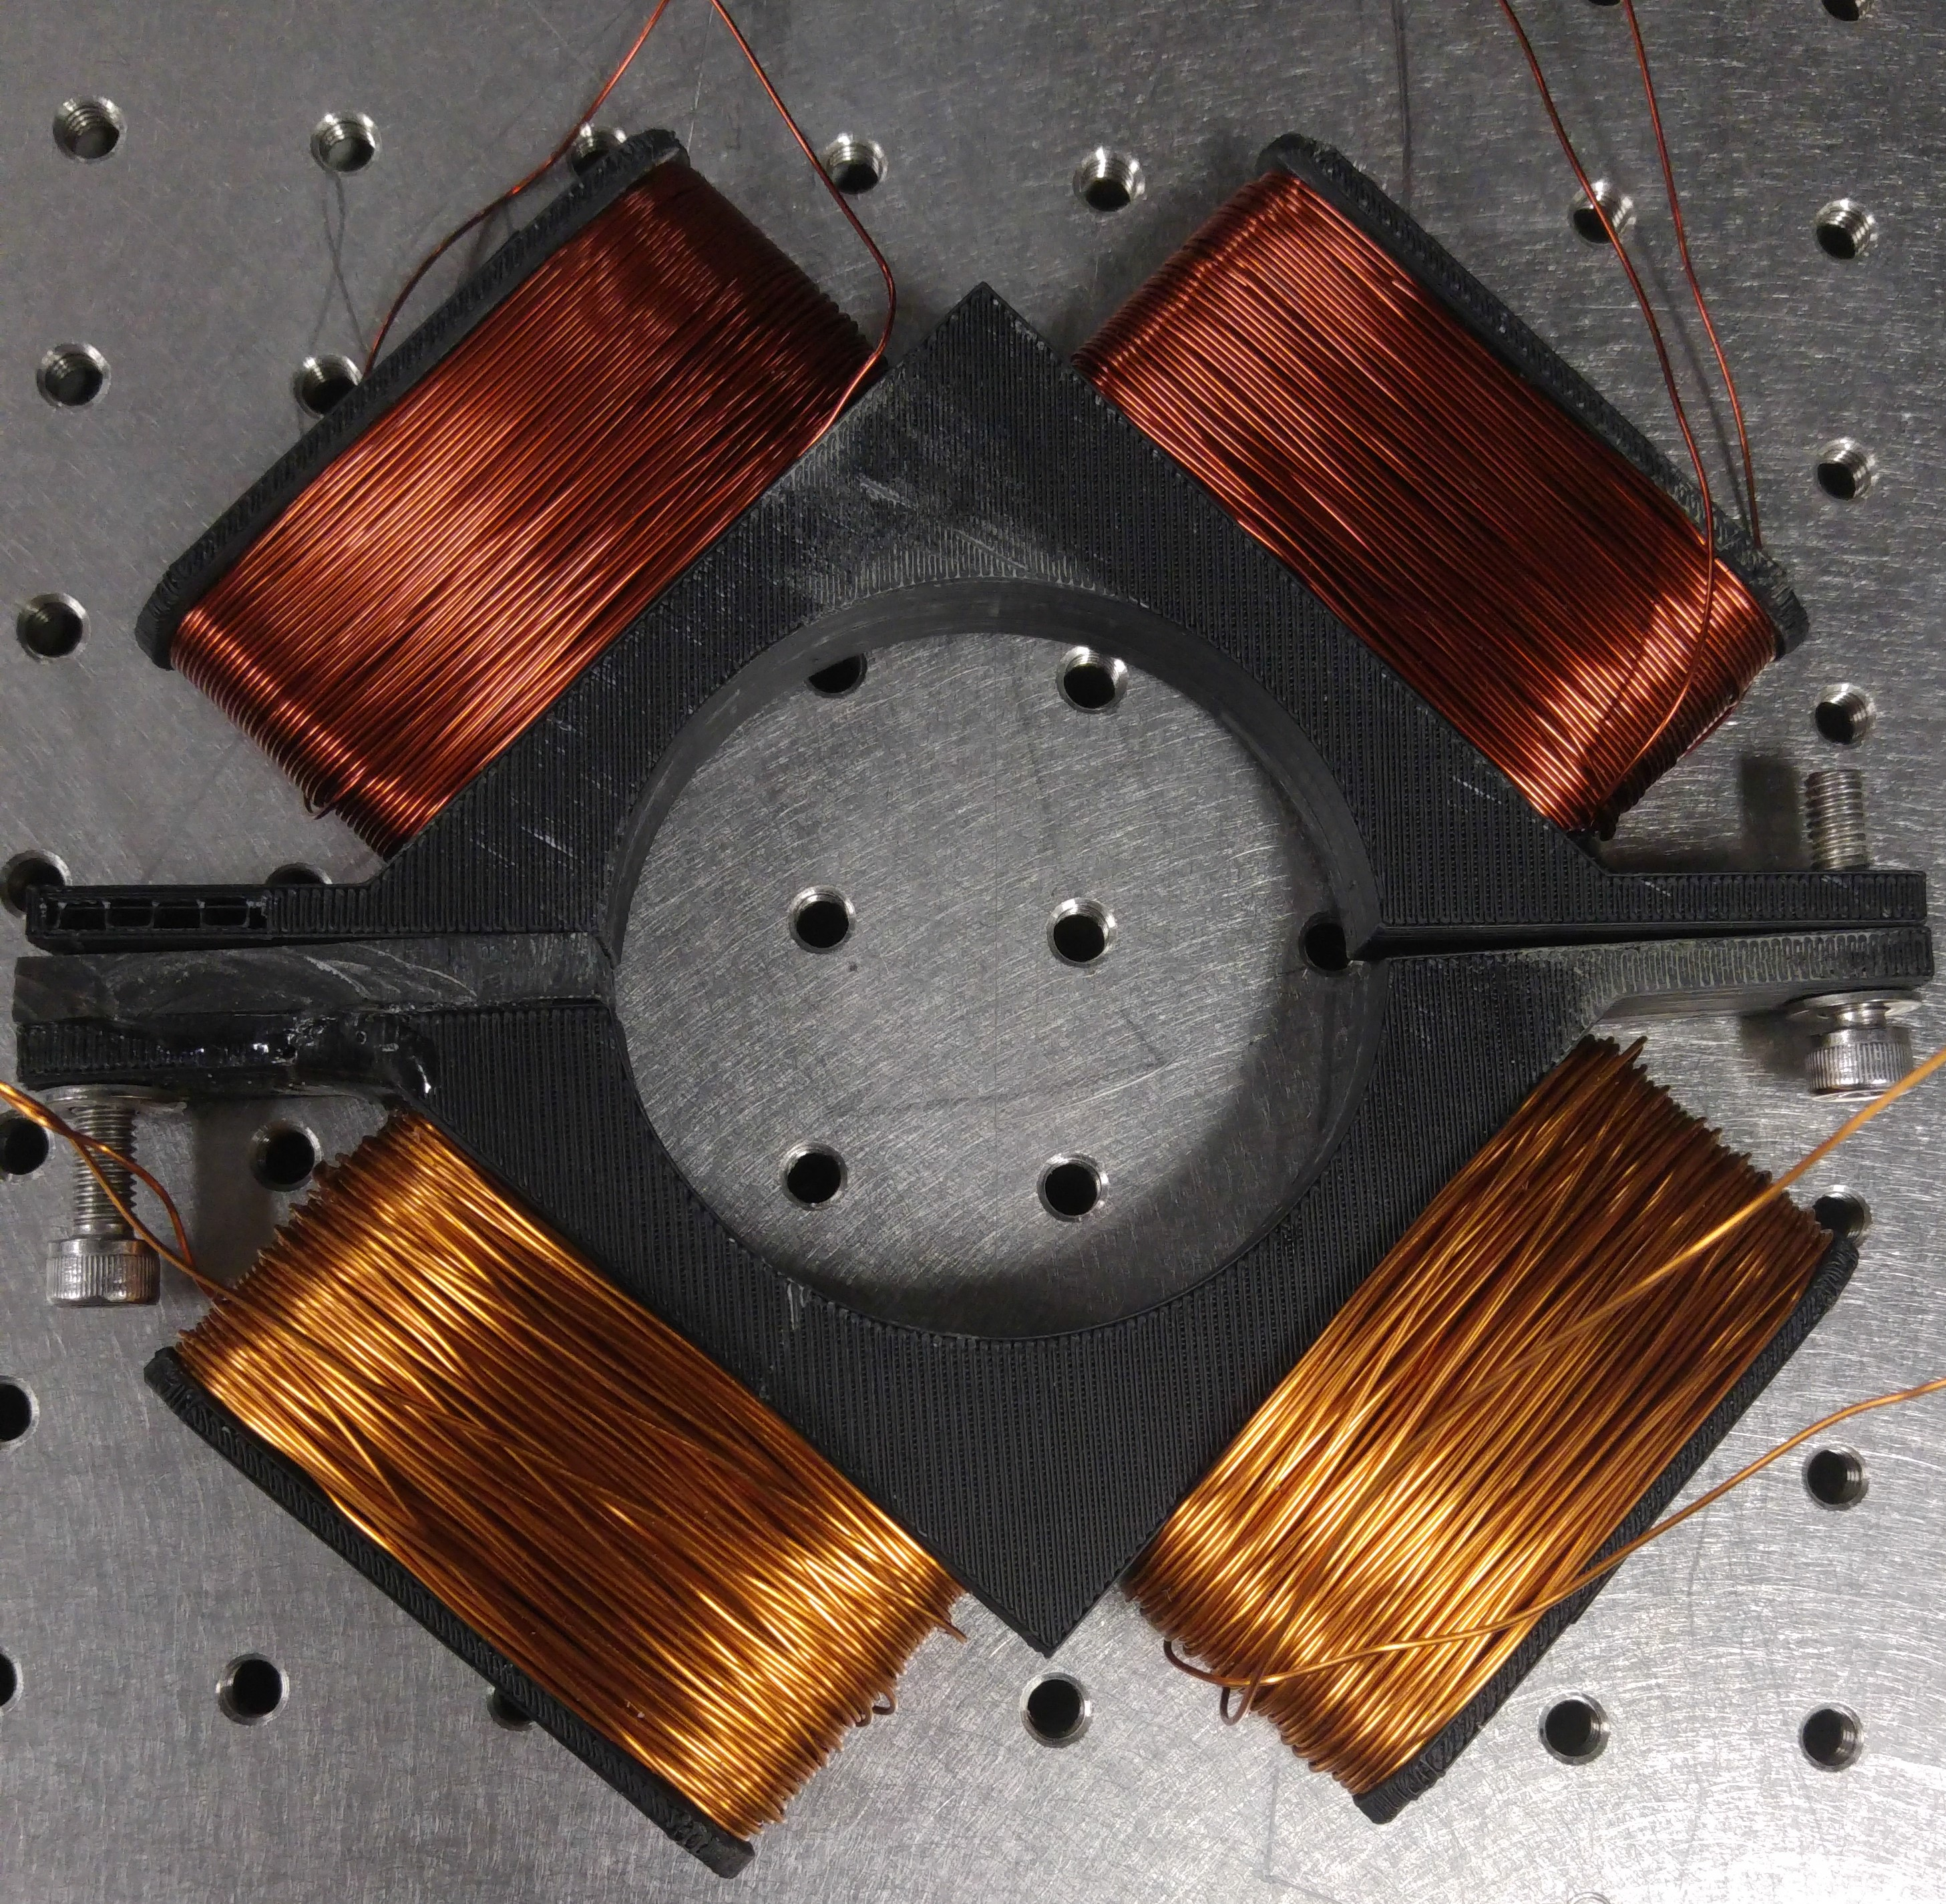
\includegraphics[width=0.5\linewidth]{part2/Figs/quadrupole.jpg}
    \caption{The 3D printed chassis was wound with copper wire to form the quadrupole lens.}
    \label{figure:quadrupole}
\end{figure}

\begin{figure}
    \centering
    \begin{subfigure}{0.49\linewidth}
    \centering
    %% Creator: Matplotlib, PGF backend
%%
%% To include the figure in your LaTeX document, write
%%   \input{<filename>.pgf}
%%
%% Make sure the required packages are loaded in your preamble
%%   \usepackage{pgf}
%%
%% Figures using additional raster images can only be included by \input if
%% they are in the same directory as the main LaTeX file. For loading figures
%% from other directories you can use the `import` package
%%   \usepackage{import}
%% and then include the figures with
%%   \import{<path to file>}{<filename>.pgf}
%%
%% Matplotlib used the following preamble
%%
\begingroup%
\makeatletter%
\begin{pgfpicture}%
\pgfpathrectangle{\pgfpointorigin}{\pgfqpoint{2.855000in}{2.284000in}}%
\pgfusepath{use as bounding box, clip}%
\begin{pgfscope}%
\pgfsetbuttcap%
\pgfsetmiterjoin%
\definecolor{currentfill}{rgb}{1.000000,1.000000,1.000000}%
\pgfsetfillcolor{currentfill}%
\pgfsetlinewidth{0.000000pt}%
\definecolor{currentstroke}{rgb}{1.000000,1.000000,1.000000}%
\pgfsetstrokecolor{currentstroke}%
\pgfsetdash{}{0pt}%
\pgfpathmoveto{\pgfqpoint{0.000000in}{0.000000in}}%
\pgfpathlineto{\pgfqpoint{2.855000in}{0.000000in}}%
\pgfpathlineto{\pgfqpoint{2.855000in}{2.284000in}}%
\pgfpathlineto{\pgfqpoint{0.000000in}{2.284000in}}%
\pgfpathclose%
\pgfusepath{fill}%
\end{pgfscope}%
\begin{pgfscope}%
\pgfsetbuttcap%
\pgfsetmiterjoin%
\definecolor{currentfill}{rgb}{1.000000,1.000000,1.000000}%
\pgfsetfillcolor{currentfill}%
\pgfsetlinewidth{0.000000pt}%
\definecolor{currentstroke}{rgb}{0.000000,0.000000,0.000000}%
\pgfsetstrokecolor{currentstroke}%
\pgfsetstrokeopacity{0.000000}%
\pgfsetdash{}{0pt}%
\pgfpathmoveto{\pgfqpoint{0.467472in}{0.521851in}}%
\pgfpathlineto{\pgfqpoint{2.670407in}{0.521851in}}%
\pgfpathlineto{\pgfqpoint{2.670407in}{2.134000in}}%
\pgfpathlineto{\pgfqpoint{0.467472in}{2.134000in}}%
\pgfpathclose%
\pgfusepath{fill}%
\end{pgfscope}%
\begin{pgfscope}%
\pgfpathrectangle{\pgfqpoint{0.467472in}{0.521851in}}{\pgfqpoint{2.202935in}{1.612149in}} %
\pgfusepath{clip}%
\pgfsetrectcap%
\pgfsetroundjoin%
\pgfsetlinewidth{1.003750pt}%
\definecolor{currentstroke}{rgb}{0.309804,0.478431,0.682353}%
\pgfsetstrokecolor{currentstroke}%
\pgfsetdash{}{0pt}%
\pgfpathmoveto{\pgfqpoint{0.467472in}{1.383105in}}%
\pgfpathlineto{\pgfqpoint{0.522546in}{1.375123in}}%
\pgfpathlineto{\pgfqpoint{0.577619in}{1.357417in}}%
\pgfpathlineto{\pgfqpoint{0.632692in}{1.354230in}}%
\pgfpathlineto{\pgfqpoint{0.687766in}{1.373191in}}%
\pgfpathlineto{\pgfqpoint{0.742839in}{1.386022in}}%
\pgfpathlineto{\pgfqpoint{0.797913in}{1.376438in}}%
\pgfpathlineto{\pgfqpoint{0.852986in}{1.355743in}}%
\pgfpathlineto{\pgfqpoint{0.908059in}{1.349822in}}%
\pgfpathlineto{\pgfqpoint{0.963133in}{1.359595in}}%
\pgfpathlineto{\pgfqpoint{1.018206in}{1.361457in}}%
\pgfpathlineto{\pgfqpoint{1.073279in}{1.341959in}}%
\pgfpathlineto{\pgfqpoint{1.128353in}{1.320422in}}%
\pgfpathlineto{\pgfqpoint{1.183426in}{1.318257in}}%
\pgfpathlineto{\pgfqpoint{1.238500in}{1.323143in}}%
\pgfpathlineto{\pgfqpoint{1.293573in}{1.307152in}}%
\pgfpathlineto{\pgfqpoint{1.348646in}{1.259918in}}%
\pgfpathlineto{\pgfqpoint{1.403720in}{1.209002in}}%
\pgfpathlineto{\pgfqpoint{1.458793in}{1.184878in}}%
\pgfpathlineto{\pgfqpoint{1.513867in}{1.182843in}}%
\pgfpathlineto{\pgfqpoint{1.568940in}{1.166394in}}%
\pgfpathlineto{\pgfqpoint{1.624013in}{1.109085in}}%
\pgfpathlineto{\pgfqpoint{1.679087in}{1.019672in}}%
\pgfpathlineto{\pgfqpoint{1.734160in}{0.924480in}}%
\pgfpathlineto{\pgfqpoint{1.789233in}{0.859874in}}%
\pgfpathlineto{\pgfqpoint{1.844307in}{0.868862in}}%
\pgfpathlineto{\pgfqpoint{1.899380in}{0.958107in}}%
\pgfpathlineto{\pgfqpoint{1.954454in}{1.084195in}}%
\pgfpathlineto{\pgfqpoint{2.009527in}{1.213254in}}%
\pgfpathlineto{\pgfqpoint{2.064600in}{1.337199in}}%
\pgfpathlineto{\pgfqpoint{2.119674in}{1.433079in}}%
\pgfpathlineto{\pgfqpoint{2.174747in}{1.490100in}}%
\pgfpathlineto{\pgfqpoint{2.229820in}{1.516367in}}%
\pgfpathlineto{\pgfqpoint{2.284894in}{1.536032in}}%
\pgfpathlineto{\pgfqpoint{2.339967in}{1.568456in}}%
\pgfpathlineto{\pgfqpoint{2.395041in}{1.617531in}}%
\pgfpathlineto{\pgfqpoint{2.450114in}{1.678346in}}%
\pgfpathlineto{\pgfqpoint{2.505187in}{1.726845in}}%
\pgfpathlineto{\pgfqpoint{2.560261in}{1.752362in}}%
\pgfpathlineto{\pgfqpoint{2.615334in}{1.762618in}}%
\pgfusepath{stroke}%
\end{pgfscope}%
\begin{pgfscope}%
\pgfpathrectangle{\pgfqpoint{0.467472in}{0.521851in}}{\pgfqpoint{2.202935in}{1.612149in}} %
\pgfusepath{clip}%
\pgfsetrectcap%
\pgfsetroundjoin%
\pgfsetlinewidth{1.003750pt}%
\definecolor{currentstroke}{rgb}{0.301961,0.607843,0.301961}%
\pgfsetstrokecolor{currentstroke}%
\pgfsetdash{}{0pt}%
\pgfpathmoveto{\pgfqpoint{0.467472in}{1.903780in}}%
\pgfpathlineto{\pgfqpoint{0.522546in}{1.944342in}}%
\pgfpathlineto{\pgfqpoint{0.577619in}{1.989825in}}%
\pgfpathlineto{\pgfqpoint{0.632692in}{1.991613in}}%
\pgfpathlineto{\pgfqpoint{0.687766in}{1.938388in}}%
\pgfpathlineto{\pgfqpoint{0.742839in}{1.897128in}}%
\pgfpathlineto{\pgfqpoint{0.797913in}{1.921071in}}%
\pgfpathlineto{\pgfqpoint{0.852986in}{1.971503in}}%
\pgfpathlineto{\pgfqpoint{0.908059in}{1.969509in}}%
\pgfpathlineto{\pgfqpoint{0.963133in}{1.914195in}}%
\pgfpathlineto{\pgfqpoint{1.018206in}{1.876969in}}%
\pgfpathlineto{\pgfqpoint{1.073279in}{1.904070in}}%
\pgfpathlineto{\pgfqpoint{1.128353in}{1.940539in}}%
\pgfpathlineto{\pgfqpoint{1.183426in}{1.906050in}}%
\pgfpathlineto{\pgfqpoint{1.238500in}{1.850436in}}%
\pgfpathlineto{\pgfqpoint{1.293573in}{1.841411in}}%
\pgfpathlineto{\pgfqpoint{1.348646in}{1.863560in}}%
\pgfpathlineto{\pgfqpoint{1.403720in}{1.879693in}}%
\pgfpathlineto{\pgfqpoint{1.458793in}{1.858548in}}%
\pgfpathlineto{\pgfqpoint{1.513867in}{1.805008in}}%
\pgfpathlineto{\pgfqpoint{1.568940in}{1.769793in}}%
\pgfpathlineto{\pgfqpoint{1.624013in}{1.772310in}}%
\pgfpathlineto{\pgfqpoint{1.679087in}{1.768062in}}%
\pgfpathlineto{\pgfqpoint{1.734160in}{1.699092in}}%
\pgfpathlineto{\pgfqpoint{1.789233in}{1.549883in}}%
\pgfpathlineto{\pgfqpoint{1.844307in}{1.353693in}}%
\pgfpathlineto{\pgfqpoint{1.899380in}{1.151764in}}%
\pgfpathlineto{\pgfqpoint{1.954454in}{0.980506in}}%
\pgfpathlineto{\pgfqpoint{2.009527in}{0.883848in}}%
\pgfpathlineto{\pgfqpoint{2.064600in}{0.886148in}}%
\pgfpathlineto{\pgfqpoint{2.119674in}{0.956946in}}%
\pgfpathlineto{\pgfqpoint{2.174747in}{1.040483in}}%
\pgfpathlineto{\pgfqpoint{2.229820in}{1.115151in}}%
\pgfpathlineto{\pgfqpoint{2.284894in}{1.196521in}}%
\pgfpathlineto{\pgfqpoint{2.339967in}{1.295350in}}%
\pgfpathlineto{\pgfqpoint{2.395041in}{1.391793in}}%
\pgfpathlineto{\pgfqpoint{2.450114in}{1.462239in}}%
\pgfpathlineto{\pgfqpoint{2.505187in}{1.494851in}}%
\pgfpathlineto{\pgfqpoint{2.560261in}{1.497397in}}%
\pgfpathlineto{\pgfqpoint{2.615334in}{1.491666in}}%
\pgfusepath{stroke}%
\end{pgfscope}%
\begin{pgfscope}%
\pgfsetrectcap%
\pgfsetmiterjoin%
\pgfsetlinewidth{1.003750pt}%
\definecolor{currentstroke}{rgb}{0.000000,0.000000,0.000000}%
\pgfsetstrokecolor{currentstroke}%
\pgfsetdash{}{0pt}%
\pgfpathmoveto{\pgfqpoint{0.467472in}{0.521851in}}%
\pgfpathlineto{\pgfqpoint{0.467472in}{2.134000in}}%
\pgfusepath{stroke}%
\end{pgfscope}%
\begin{pgfscope}%
\pgfsetrectcap%
\pgfsetmiterjoin%
\pgfsetlinewidth{1.003750pt}%
\definecolor{currentstroke}{rgb}{0.000000,0.000000,0.000000}%
\pgfsetstrokecolor{currentstroke}%
\pgfsetdash{}{0pt}%
\pgfpathmoveto{\pgfqpoint{0.467472in}{2.134000in}}%
\pgfpathlineto{\pgfqpoint{2.670407in}{2.134000in}}%
\pgfusepath{stroke}%
\end{pgfscope}%
\begin{pgfscope}%
\pgfsetrectcap%
\pgfsetmiterjoin%
\pgfsetlinewidth{1.003750pt}%
\definecolor{currentstroke}{rgb}{0.000000,0.000000,0.000000}%
\pgfsetstrokecolor{currentstroke}%
\pgfsetdash{}{0pt}%
\pgfpathmoveto{\pgfqpoint{0.467472in}{0.521851in}}%
\pgfpathlineto{\pgfqpoint{2.670407in}{0.521851in}}%
\pgfusepath{stroke}%
\end{pgfscope}%
\begin{pgfscope}%
\pgfsetrectcap%
\pgfsetmiterjoin%
\pgfsetlinewidth{1.003750pt}%
\definecolor{currentstroke}{rgb}{0.000000,0.000000,0.000000}%
\pgfsetstrokecolor{currentstroke}%
\pgfsetdash{}{0pt}%
\pgfpathmoveto{\pgfqpoint{2.670407in}{0.521851in}}%
\pgfpathlineto{\pgfqpoint{2.670407in}{2.134000in}}%
\pgfusepath{stroke}%
\end{pgfscope}%
\begin{pgfscope}%
\pgfsetbuttcap%
\pgfsetroundjoin%
\definecolor{currentfill}{rgb}{0.000000,0.000000,0.000000}%
\pgfsetfillcolor{currentfill}%
\pgfsetlinewidth{0.501875pt}%
\definecolor{currentstroke}{rgb}{0.000000,0.000000,0.000000}%
\pgfsetstrokecolor{currentstroke}%
\pgfsetdash{}{0pt}%
\pgfsys@defobject{currentmarker}{\pgfqpoint{0.000000in}{0.000000in}}{\pgfqpoint{0.000000in}{0.055556in}}{%
\pgfpathmoveto{\pgfqpoint{0.000000in}{0.000000in}}%
\pgfpathlineto{\pgfqpoint{0.000000in}{0.055556in}}%
\pgfusepath{stroke,fill}%
}%
\begin{pgfscope}%
\pgfsys@transformshift{0.467472in}{0.521851in}%
\pgfsys@useobject{currentmarker}{}%
\end{pgfscope}%
\end{pgfscope}%
\begin{pgfscope}%
\pgfsetbuttcap%
\pgfsetroundjoin%
\definecolor{currentfill}{rgb}{0.000000,0.000000,0.000000}%
\pgfsetfillcolor{currentfill}%
\pgfsetlinewidth{0.501875pt}%
\definecolor{currentstroke}{rgb}{0.000000,0.000000,0.000000}%
\pgfsetstrokecolor{currentstroke}%
\pgfsetdash{}{0pt}%
\pgfsys@defobject{currentmarker}{\pgfqpoint{0.000000in}{-0.055556in}}{\pgfqpoint{0.000000in}{0.000000in}}{%
\pgfpathmoveto{\pgfqpoint{0.000000in}{0.000000in}}%
\pgfpathlineto{\pgfqpoint{0.000000in}{-0.055556in}}%
\pgfusepath{stroke,fill}%
}%
\begin{pgfscope}%
\pgfsys@transformshift{0.467472in}{2.134000in}%
\pgfsys@useobject{currentmarker}{}%
\end{pgfscope}%
\end{pgfscope}%
\begin{pgfscope}%
\pgftext[x=0.467472in,y=0.466296in,,top]{\fontsize{10.000000}{12.000000}\selectfont \(\displaystyle 0\)}%
\end{pgfscope}%
\begin{pgfscope}%
\pgfsetbuttcap%
\pgfsetroundjoin%
\definecolor{currentfill}{rgb}{0.000000,0.000000,0.000000}%
\pgfsetfillcolor{currentfill}%
\pgfsetlinewidth{0.501875pt}%
\definecolor{currentstroke}{rgb}{0.000000,0.000000,0.000000}%
\pgfsetstrokecolor{currentstroke}%
\pgfsetdash{}{0pt}%
\pgfsys@defobject{currentmarker}{\pgfqpoint{0.000000in}{0.000000in}}{\pgfqpoint{0.000000in}{0.055556in}}{%
\pgfpathmoveto{\pgfqpoint{0.000000in}{0.000000in}}%
\pgfpathlineto{\pgfqpoint{0.000000in}{0.055556in}}%
\pgfusepath{stroke,fill}%
}%
\begin{pgfscope}%
\pgfsys@transformshift{1.018206in}{0.521851in}%
\pgfsys@useobject{currentmarker}{}%
\end{pgfscope}%
\end{pgfscope}%
\begin{pgfscope}%
\pgfsetbuttcap%
\pgfsetroundjoin%
\definecolor{currentfill}{rgb}{0.000000,0.000000,0.000000}%
\pgfsetfillcolor{currentfill}%
\pgfsetlinewidth{0.501875pt}%
\definecolor{currentstroke}{rgb}{0.000000,0.000000,0.000000}%
\pgfsetstrokecolor{currentstroke}%
\pgfsetdash{}{0pt}%
\pgfsys@defobject{currentmarker}{\pgfqpoint{0.000000in}{-0.055556in}}{\pgfqpoint{0.000000in}{0.000000in}}{%
\pgfpathmoveto{\pgfqpoint{0.000000in}{0.000000in}}%
\pgfpathlineto{\pgfqpoint{0.000000in}{-0.055556in}}%
\pgfusepath{stroke,fill}%
}%
\begin{pgfscope}%
\pgfsys@transformshift{1.018206in}{2.134000in}%
\pgfsys@useobject{currentmarker}{}%
\end{pgfscope}%
\end{pgfscope}%
\begin{pgfscope}%
\pgftext[x=1.018206in,y=0.466296in,,top]{\fontsize{10.000000}{12.000000}\selectfont \(\displaystyle 1\)}%
\end{pgfscope}%
\begin{pgfscope}%
\pgfsetbuttcap%
\pgfsetroundjoin%
\definecolor{currentfill}{rgb}{0.000000,0.000000,0.000000}%
\pgfsetfillcolor{currentfill}%
\pgfsetlinewidth{0.501875pt}%
\definecolor{currentstroke}{rgb}{0.000000,0.000000,0.000000}%
\pgfsetstrokecolor{currentstroke}%
\pgfsetdash{}{0pt}%
\pgfsys@defobject{currentmarker}{\pgfqpoint{0.000000in}{0.000000in}}{\pgfqpoint{0.000000in}{0.055556in}}{%
\pgfpathmoveto{\pgfqpoint{0.000000in}{0.000000in}}%
\pgfpathlineto{\pgfqpoint{0.000000in}{0.055556in}}%
\pgfusepath{stroke,fill}%
}%
\begin{pgfscope}%
\pgfsys@transformshift{1.568940in}{0.521851in}%
\pgfsys@useobject{currentmarker}{}%
\end{pgfscope}%
\end{pgfscope}%
\begin{pgfscope}%
\pgfsetbuttcap%
\pgfsetroundjoin%
\definecolor{currentfill}{rgb}{0.000000,0.000000,0.000000}%
\pgfsetfillcolor{currentfill}%
\pgfsetlinewidth{0.501875pt}%
\definecolor{currentstroke}{rgb}{0.000000,0.000000,0.000000}%
\pgfsetstrokecolor{currentstroke}%
\pgfsetdash{}{0pt}%
\pgfsys@defobject{currentmarker}{\pgfqpoint{0.000000in}{-0.055556in}}{\pgfqpoint{0.000000in}{0.000000in}}{%
\pgfpathmoveto{\pgfqpoint{0.000000in}{0.000000in}}%
\pgfpathlineto{\pgfqpoint{0.000000in}{-0.055556in}}%
\pgfusepath{stroke,fill}%
}%
\begin{pgfscope}%
\pgfsys@transformshift{1.568940in}{2.134000in}%
\pgfsys@useobject{currentmarker}{}%
\end{pgfscope}%
\end{pgfscope}%
\begin{pgfscope}%
\pgftext[x=1.568940in,y=0.466296in,,top]{\fontsize{10.000000}{12.000000}\selectfont \(\displaystyle 2\)}%
\end{pgfscope}%
\begin{pgfscope}%
\pgfsetbuttcap%
\pgfsetroundjoin%
\definecolor{currentfill}{rgb}{0.000000,0.000000,0.000000}%
\pgfsetfillcolor{currentfill}%
\pgfsetlinewidth{0.501875pt}%
\definecolor{currentstroke}{rgb}{0.000000,0.000000,0.000000}%
\pgfsetstrokecolor{currentstroke}%
\pgfsetdash{}{0pt}%
\pgfsys@defobject{currentmarker}{\pgfqpoint{0.000000in}{0.000000in}}{\pgfqpoint{0.000000in}{0.055556in}}{%
\pgfpathmoveto{\pgfqpoint{0.000000in}{0.000000in}}%
\pgfpathlineto{\pgfqpoint{0.000000in}{0.055556in}}%
\pgfusepath{stroke,fill}%
}%
\begin{pgfscope}%
\pgfsys@transformshift{2.119674in}{0.521851in}%
\pgfsys@useobject{currentmarker}{}%
\end{pgfscope}%
\end{pgfscope}%
\begin{pgfscope}%
\pgfsetbuttcap%
\pgfsetroundjoin%
\definecolor{currentfill}{rgb}{0.000000,0.000000,0.000000}%
\pgfsetfillcolor{currentfill}%
\pgfsetlinewidth{0.501875pt}%
\definecolor{currentstroke}{rgb}{0.000000,0.000000,0.000000}%
\pgfsetstrokecolor{currentstroke}%
\pgfsetdash{}{0pt}%
\pgfsys@defobject{currentmarker}{\pgfqpoint{0.000000in}{-0.055556in}}{\pgfqpoint{0.000000in}{0.000000in}}{%
\pgfpathmoveto{\pgfqpoint{0.000000in}{0.000000in}}%
\pgfpathlineto{\pgfqpoint{0.000000in}{-0.055556in}}%
\pgfusepath{stroke,fill}%
}%
\begin{pgfscope}%
\pgfsys@transformshift{2.119674in}{2.134000in}%
\pgfsys@useobject{currentmarker}{}%
\end{pgfscope}%
\end{pgfscope}%
\begin{pgfscope}%
\pgftext[x=2.119674in,y=0.466296in,,top]{\fontsize{10.000000}{12.000000}\selectfont \(\displaystyle 3\)}%
\end{pgfscope}%
\begin{pgfscope}%
\pgfsetbuttcap%
\pgfsetroundjoin%
\definecolor{currentfill}{rgb}{0.000000,0.000000,0.000000}%
\pgfsetfillcolor{currentfill}%
\pgfsetlinewidth{0.501875pt}%
\definecolor{currentstroke}{rgb}{0.000000,0.000000,0.000000}%
\pgfsetstrokecolor{currentstroke}%
\pgfsetdash{}{0pt}%
\pgfsys@defobject{currentmarker}{\pgfqpoint{0.000000in}{0.000000in}}{\pgfqpoint{0.000000in}{0.055556in}}{%
\pgfpathmoveto{\pgfqpoint{0.000000in}{0.000000in}}%
\pgfpathlineto{\pgfqpoint{0.000000in}{0.055556in}}%
\pgfusepath{stroke,fill}%
}%
\begin{pgfscope}%
\pgfsys@transformshift{2.670407in}{0.521851in}%
\pgfsys@useobject{currentmarker}{}%
\end{pgfscope}%
\end{pgfscope}%
\begin{pgfscope}%
\pgfsetbuttcap%
\pgfsetroundjoin%
\definecolor{currentfill}{rgb}{0.000000,0.000000,0.000000}%
\pgfsetfillcolor{currentfill}%
\pgfsetlinewidth{0.501875pt}%
\definecolor{currentstroke}{rgb}{0.000000,0.000000,0.000000}%
\pgfsetstrokecolor{currentstroke}%
\pgfsetdash{}{0pt}%
\pgfsys@defobject{currentmarker}{\pgfqpoint{0.000000in}{-0.055556in}}{\pgfqpoint{0.000000in}{0.000000in}}{%
\pgfpathmoveto{\pgfqpoint{0.000000in}{0.000000in}}%
\pgfpathlineto{\pgfqpoint{0.000000in}{-0.055556in}}%
\pgfusepath{stroke,fill}%
}%
\begin{pgfscope}%
\pgfsys@transformshift{2.670407in}{2.134000in}%
\pgfsys@useobject{currentmarker}{}%
\end{pgfscope}%
\end{pgfscope}%
\begin{pgfscope}%
\pgftext[x=2.670407in,y=0.466296in,,top]{\fontsize{10.000000}{12.000000}\selectfont \(\displaystyle 4\)}%
\end{pgfscope}%
\begin{pgfscope}%
\pgftext[x=1.568940in,y=0.273395in,,top]{\fontsize{10.000000}{12.000000}\selectfont Einzel Lens Voltage (kV)}%
\end{pgfscope}%
\begin{pgfscope}%
\pgfsetbuttcap%
\pgfsetroundjoin%
\definecolor{currentfill}{rgb}{0.000000,0.000000,0.000000}%
\pgfsetfillcolor{currentfill}%
\pgfsetlinewidth{0.501875pt}%
\definecolor{currentstroke}{rgb}{0.000000,0.000000,0.000000}%
\pgfsetstrokecolor{currentstroke}%
\pgfsetdash{}{0pt}%
\pgfsys@defobject{currentmarker}{\pgfqpoint{0.000000in}{0.000000in}}{\pgfqpoint{0.055556in}{0.000000in}}{%
\pgfpathmoveto{\pgfqpoint{0.000000in}{0.000000in}}%
\pgfpathlineto{\pgfqpoint{0.055556in}{0.000000in}}%
\pgfusepath{stroke,fill}%
}%
\begin{pgfscope}%
\pgfsys@transformshift{0.467472in}{0.521851in}%
\pgfsys@useobject{currentmarker}{}%
\end{pgfscope}%
\end{pgfscope}%
\begin{pgfscope}%
\pgfsetbuttcap%
\pgfsetroundjoin%
\definecolor{currentfill}{rgb}{0.000000,0.000000,0.000000}%
\pgfsetfillcolor{currentfill}%
\pgfsetlinewidth{0.501875pt}%
\definecolor{currentstroke}{rgb}{0.000000,0.000000,0.000000}%
\pgfsetstrokecolor{currentstroke}%
\pgfsetdash{}{0pt}%
\pgfsys@defobject{currentmarker}{\pgfqpoint{-0.055556in}{0.000000in}}{\pgfqpoint{0.000000in}{0.000000in}}{%
\pgfpathmoveto{\pgfqpoint{0.000000in}{0.000000in}}%
\pgfpathlineto{\pgfqpoint{-0.055556in}{0.000000in}}%
\pgfusepath{stroke,fill}%
}%
\begin{pgfscope}%
\pgfsys@transformshift{2.670407in}{0.521851in}%
\pgfsys@useobject{currentmarker}{}%
\end{pgfscope}%
\end{pgfscope}%
\begin{pgfscope}%
\pgftext[x=0.411917in,y=0.521851in,right,]{\fontsize{10.000000}{12.000000}\selectfont \(\displaystyle 0\)}%
\end{pgfscope}%
\begin{pgfscope}%
\pgfsetbuttcap%
\pgfsetroundjoin%
\definecolor{currentfill}{rgb}{0.000000,0.000000,0.000000}%
\pgfsetfillcolor{currentfill}%
\pgfsetlinewidth{0.501875pt}%
\definecolor{currentstroke}{rgb}{0.000000,0.000000,0.000000}%
\pgfsetstrokecolor{currentstroke}%
\pgfsetdash{}{0pt}%
\pgfsys@defobject{currentmarker}{\pgfqpoint{0.000000in}{0.000000in}}{\pgfqpoint{0.055556in}{0.000000in}}{%
\pgfpathmoveto{\pgfqpoint{0.000000in}{0.000000in}}%
\pgfpathlineto{\pgfqpoint{0.055556in}{0.000000in}}%
\pgfusepath{stroke,fill}%
}%
\begin{pgfscope}%
\pgfsys@transformshift{0.467472in}{0.880107in}%
\pgfsys@useobject{currentmarker}{}%
\end{pgfscope}%
\end{pgfscope}%
\begin{pgfscope}%
\pgfsetbuttcap%
\pgfsetroundjoin%
\definecolor{currentfill}{rgb}{0.000000,0.000000,0.000000}%
\pgfsetfillcolor{currentfill}%
\pgfsetlinewidth{0.501875pt}%
\definecolor{currentstroke}{rgb}{0.000000,0.000000,0.000000}%
\pgfsetstrokecolor{currentstroke}%
\pgfsetdash{}{0pt}%
\pgfsys@defobject{currentmarker}{\pgfqpoint{-0.055556in}{0.000000in}}{\pgfqpoint{0.000000in}{0.000000in}}{%
\pgfpathmoveto{\pgfqpoint{0.000000in}{0.000000in}}%
\pgfpathlineto{\pgfqpoint{-0.055556in}{0.000000in}}%
\pgfusepath{stroke,fill}%
}%
\begin{pgfscope}%
\pgfsys@transformshift{2.670407in}{0.880107in}%
\pgfsys@useobject{currentmarker}{}%
\end{pgfscope}%
\end{pgfscope}%
\begin{pgfscope}%
\pgftext[x=0.411917in,y=0.880107in,right,]{\fontsize{10.000000}{12.000000}\selectfont \(\displaystyle 1\)}%
\end{pgfscope}%
\begin{pgfscope}%
\pgfsetbuttcap%
\pgfsetroundjoin%
\definecolor{currentfill}{rgb}{0.000000,0.000000,0.000000}%
\pgfsetfillcolor{currentfill}%
\pgfsetlinewidth{0.501875pt}%
\definecolor{currentstroke}{rgb}{0.000000,0.000000,0.000000}%
\pgfsetstrokecolor{currentstroke}%
\pgfsetdash{}{0pt}%
\pgfsys@defobject{currentmarker}{\pgfqpoint{0.000000in}{0.000000in}}{\pgfqpoint{0.055556in}{0.000000in}}{%
\pgfpathmoveto{\pgfqpoint{0.000000in}{0.000000in}}%
\pgfpathlineto{\pgfqpoint{0.055556in}{0.000000in}}%
\pgfusepath{stroke,fill}%
}%
\begin{pgfscope}%
\pgfsys@transformshift{0.467472in}{1.238362in}%
\pgfsys@useobject{currentmarker}{}%
\end{pgfscope}%
\end{pgfscope}%
\begin{pgfscope}%
\pgfsetbuttcap%
\pgfsetroundjoin%
\definecolor{currentfill}{rgb}{0.000000,0.000000,0.000000}%
\pgfsetfillcolor{currentfill}%
\pgfsetlinewidth{0.501875pt}%
\definecolor{currentstroke}{rgb}{0.000000,0.000000,0.000000}%
\pgfsetstrokecolor{currentstroke}%
\pgfsetdash{}{0pt}%
\pgfsys@defobject{currentmarker}{\pgfqpoint{-0.055556in}{0.000000in}}{\pgfqpoint{0.000000in}{0.000000in}}{%
\pgfpathmoveto{\pgfqpoint{0.000000in}{0.000000in}}%
\pgfpathlineto{\pgfqpoint{-0.055556in}{0.000000in}}%
\pgfusepath{stroke,fill}%
}%
\begin{pgfscope}%
\pgfsys@transformshift{2.670407in}{1.238362in}%
\pgfsys@useobject{currentmarker}{}%
\end{pgfscope}%
\end{pgfscope}%
\begin{pgfscope}%
\pgftext[x=0.411917in,y=1.238362in,right,]{\fontsize{10.000000}{12.000000}\selectfont \(\displaystyle 2\)}%
\end{pgfscope}%
\begin{pgfscope}%
\pgfsetbuttcap%
\pgfsetroundjoin%
\definecolor{currentfill}{rgb}{0.000000,0.000000,0.000000}%
\pgfsetfillcolor{currentfill}%
\pgfsetlinewidth{0.501875pt}%
\definecolor{currentstroke}{rgb}{0.000000,0.000000,0.000000}%
\pgfsetstrokecolor{currentstroke}%
\pgfsetdash{}{0pt}%
\pgfsys@defobject{currentmarker}{\pgfqpoint{0.000000in}{0.000000in}}{\pgfqpoint{0.055556in}{0.000000in}}{%
\pgfpathmoveto{\pgfqpoint{0.000000in}{0.000000in}}%
\pgfpathlineto{\pgfqpoint{0.055556in}{0.000000in}}%
\pgfusepath{stroke,fill}%
}%
\begin{pgfscope}%
\pgfsys@transformshift{0.467472in}{1.596617in}%
\pgfsys@useobject{currentmarker}{}%
\end{pgfscope}%
\end{pgfscope}%
\begin{pgfscope}%
\pgfsetbuttcap%
\pgfsetroundjoin%
\definecolor{currentfill}{rgb}{0.000000,0.000000,0.000000}%
\pgfsetfillcolor{currentfill}%
\pgfsetlinewidth{0.501875pt}%
\definecolor{currentstroke}{rgb}{0.000000,0.000000,0.000000}%
\pgfsetstrokecolor{currentstroke}%
\pgfsetdash{}{0pt}%
\pgfsys@defobject{currentmarker}{\pgfqpoint{-0.055556in}{0.000000in}}{\pgfqpoint{0.000000in}{0.000000in}}{%
\pgfpathmoveto{\pgfqpoint{0.000000in}{0.000000in}}%
\pgfpathlineto{\pgfqpoint{-0.055556in}{0.000000in}}%
\pgfusepath{stroke,fill}%
}%
\begin{pgfscope}%
\pgfsys@transformshift{2.670407in}{1.596617in}%
\pgfsys@useobject{currentmarker}{}%
\end{pgfscope}%
\end{pgfscope}%
\begin{pgfscope}%
\pgftext[x=0.411917in,y=1.596617in,right,]{\fontsize{10.000000}{12.000000}\selectfont \(\displaystyle 3\)}%
\end{pgfscope}%
\begin{pgfscope}%
\pgfsetbuttcap%
\pgfsetroundjoin%
\definecolor{currentfill}{rgb}{0.000000,0.000000,0.000000}%
\pgfsetfillcolor{currentfill}%
\pgfsetlinewidth{0.501875pt}%
\definecolor{currentstroke}{rgb}{0.000000,0.000000,0.000000}%
\pgfsetstrokecolor{currentstroke}%
\pgfsetdash{}{0pt}%
\pgfsys@defobject{currentmarker}{\pgfqpoint{0.000000in}{0.000000in}}{\pgfqpoint{0.055556in}{0.000000in}}{%
\pgfpathmoveto{\pgfqpoint{0.000000in}{0.000000in}}%
\pgfpathlineto{\pgfqpoint{0.055556in}{0.000000in}}%
\pgfusepath{stroke,fill}%
}%
\begin{pgfscope}%
\pgfsys@transformshift{0.467472in}{1.954872in}%
\pgfsys@useobject{currentmarker}{}%
\end{pgfscope}%
\end{pgfscope}%
\begin{pgfscope}%
\pgfsetbuttcap%
\pgfsetroundjoin%
\definecolor{currentfill}{rgb}{0.000000,0.000000,0.000000}%
\pgfsetfillcolor{currentfill}%
\pgfsetlinewidth{0.501875pt}%
\definecolor{currentstroke}{rgb}{0.000000,0.000000,0.000000}%
\pgfsetstrokecolor{currentstroke}%
\pgfsetdash{}{0pt}%
\pgfsys@defobject{currentmarker}{\pgfqpoint{-0.055556in}{0.000000in}}{\pgfqpoint{0.000000in}{0.000000in}}{%
\pgfpathmoveto{\pgfqpoint{0.000000in}{0.000000in}}%
\pgfpathlineto{\pgfqpoint{-0.055556in}{0.000000in}}%
\pgfusepath{stroke,fill}%
}%
\begin{pgfscope}%
\pgfsys@transformshift{2.670407in}{1.954872in}%
\pgfsys@useobject{currentmarker}{}%
\end{pgfscope}%
\end{pgfscope}%
\begin{pgfscope}%
\pgftext[x=0.411917in,y=1.954872in,right,]{\fontsize{10.000000}{12.000000}\selectfont \(\displaystyle 4\)}%
\end{pgfscope}%
\begin{pgfscope}%
\pgftext[x=0.273028in,y=1.327926in,,bottom,rotate=90.000000]{\fontsize{10.000000}{12.000000}\selectfont RMS Beam Size (mm)}%
\end{pgfscope}%
\begin{pgfscope}%
\definecolor{textcolor}{rgb}{0.309804,0.478431,0.682353}%
\pgfsetstrokecolor{textcolor}%
\pgfsetfillcolor{textcolor}%
\pgftext[x=1.679087in,y=0.715309in,left,base]{\color{textcolor}\fontsize{10.000000}{12.000000}\selectfont x-axis}%
\end{pgfscope}%
\begin{pgfscope}%
\definecolor{textcolor}{rgb}{0.301961,0.607843,0.301961}%
\pgfsetstrokecolor{textcolor}%
\pgfsetfillcolor{textcolor}%
\pgftext[x=1.679087in,y=1.940542in,left,base]{\color{textcolor}\fontsize{10.000000}{12.000000}\selectfont y-axis}%
\end{pgfscope}%
\begin{pgfscope}%
\pgfsetbuttcap%
\pgfsetmiterjoin%
\definecolor{currentfill}{rgb}{1.000000,1.000000,1.000000}%
\pgfsetfillcolor{currentfill}%
\pgfsetlinewidth{0.000000pt}%
\definecolor{currentstroke}{rgb}{0.000000,0.000000,0.000000}%
\pgfsetstrokecolor{currentstroke}%
\pgfsetstrokeopacity{0.000000}%
\pgfsetdash{}{0pt}%
\pgfpathmoveto{\pgfqpoint{0.528175in}{0.593840in}}%
\pgfpathlineto{\pgfqpoint{0.984975in}{0.593840in}}%
\pgfpathlineto{\pgfqpoint{0.984975in}{1.050640in}}%
\pgfpathlineto{\pgfqpoint{0.528175in}{1.050640in}}%
\pgfpathclose%
\pgfusepath{fill}%
\end{pgfscope}%
\begin{pgfscope}%
\pgfpathrectangle{\pgfqpoint{0.528175in}{0.593840in}}{\pgfqpoint{0.456800in}{0.456800in}} %
\pgfusepath{clip}%
\pgftext[at=\pgfqpoint{0.528175in}{0.593840in},left,bottom]{\pgfimage[interpolate=true,width=0.460000in,height=0.470000in]{quadrupole_off-img0.png}}%
\end{pgfscope}%
\begin{pgfscope}%
\pgfsetrectcap%
\pgfsetmiterjoin%
\pgfsetlinewidth{1.003750pt}%
\definecolor{currentstroke}{rgb}{0.000000,0.000000,0.000000}%
\pgfsetstrokecolor{currentstroke}%
\pgfsetdash{}{0pt}%
\pgfpathmoveto{\pgfqpoint{0.528175in}{0.593840in}}%
\pgfpathlineto{\pgfqpoint{0.528175in}{1.050640in}}%
\pgfusepath{stroke}%
\end{pgfscope}%
\begin{pgfscope}%
\pgfsetrectcap%
\pgfsetmiterjoin%
\pgfsetlinewidth{1.003750pt}%
\definecolor{currentstroke}{rgb}{0.000000,0.000000,0.000000}%
\pgfsetstrokecolor{currentstroke}%
\pgfsetdash{}{0pt}%
\pgfpathmoveto{\pgfqpoint{0.528175in}{1.050640in}}%
\pgfpathlineto{\pgfqpoint{0.984975in}{1.050640in}}%
\pgfusepath{stroke}%
\end{pgfscope}%
\begin{pgfscope}%
\pgfsetrectcap%
\pgfsetmiterjoin%
\pgfsetlinewidth{1.003750pt}%
\definecolor{currentstroke}{rgb}{0.000000,0.000000,0.000000}%
\pgfsetstrokecolor{currentstroke}%
\pgfsetdash{}{0pt}%
\pgfpathmoveto{\pgfqpoint{0.528175in}{0.593840in}}%
\pgfpathlineto{\pgfqpoint{0.984975in}{0.593840in}}%
\pgfusepath{stroke}%
\end{pgfscope}%
\begin{pgfscope}%
\pgfsetrectcap%
\pgfsetmiterjoin%
\pgfsetlinewidth{1.003750pt}%
\definecolor{currentstroke}{rgb}{0.000000,0.000000,0.000000}%
\pgfsetstrokecolor{currentstroke}%
\pgfsetdash{}{0pt}%
\pgfpathmoveto{\pgfqpoint{0.984975in}{0.593840in}}%
\pgfpathlineto{\pgfqpoint{0.984975in}{1.050640in}}%
\pgfusepath{stroke}%
\end{pgfscope}%
\begin{pgfscope}%
\pgfsetbuttcap%
\pgfsetmiterjoin%
\definecolor{currentfill}{rgb}{1.000000,1.000000,1.000000}%
\pgfsetfillcolor{currentfill}%
\pgfsetlinewidth{0.000000pt}%
\definecolor{currentstroke}{rgb}{0.000000,0.000000,0.000000}%
\pgfsetstrokecolor{currentstroke}%
\pgfsetstrokeopacity{0.000000}%
\pgfsetdash{}{0pt}%
\pgfpathmoveto{\pgfqpoint{1.027800in}{0.593840in}}%
\pgfpathlineto{\pgfqpoint{1.484600in}{0.593840in}}%
\pgfpathlineto{\pgfqpoint{1.484600in}{1.050640in}}%
\pgfpathlineto{\pgfqpoint{1.027800in}{1.050640in}}%
\pgfpathclose%
\pgfusepath{fill}%
\end{pgfscope}%
\begin{pgfscope}%
\pgfpathrectangle{\pgfqpoint{1.027800in}{0.593840in}}{\pgfqpoint{0.456800in}{0.456800in}} %
\pgfusepath{clip}%
\pgftext[at=\pgfqpoint{1.027800in}{0.593840in},left,bottom]{\pgfimage[interpolate=true,width=0.460000in,height=0.470000in]{quadrupole_off-img1.png}}%
\end{pgfscope}%
\begin{pgfscope}%
\pgfsetrectcap%
\pgfsetmiterjoin%
\pgfsetlinewidth{1.003750pt}%
\definecolor{currentstroke}{rgb}{0.000000,0.000000,0.000000}%
\pgfsetstrokecolor{currentstroke}%
\pgfsetdash{}{0pt}%
\pgfpathmoveto{\pgfqpoint{1.027800in}{0.593840in}}%
\pgfpathlineto{\pgfqpoint{1.027800in}{1.050640in}}%
\pgfusepath{stroke}%
\end{pgfscope}%
\begin{pgfscope}%
\pgfsetrectcap%
\pgfsetmiterjoin%
\pgfsetlinewidth{1.003750pt}%
\definecolor{currentstroke}{rgb}{0.000000,0.000000,0.000000}%
\pgfsetstrokecolor{currentstroke}%
\pgfsetdash{}{0pt}%
\pgfpathmoveto{\pgfqpoint{1.027800in}{1.050640in}}%
\pgfpathlineto{\pgfqpoint{1.484600in}{1.050640in}}%
\pgfusepath{stroke}%
\end{pgfscope}%
\begin{pgfscope}%
\pgfsetrectcap%
\pgfsetmiterjoin%
\pgfsetlinewidth{1.003750pt}%
\definecolor{currentstroke}{rgb}{0.000000,0.000000,0.000000}%
\pgfsetstrokecolor{currentstroke}%
\pgfsetdash{}{0pt}%
\pgfpathmoveto{\pgfqpoint{1.027800in}{0.593840in}}%
\pgfpathlineto{\pgfqpoint{1.484600in}{0.593840in}}%
\pgfusepath{stroke}%
\end{pgfscope}%
\begin{pgfscope}%
\pgfsetrectcap%
\pgfsetmiterjoin%
\pgfsetlinewidth{1.003750pt}%
\definecolor{currentstroke}{rgb}{0.000000,0.000000,0.000000}%
\pgfsetstrokecolor{currentstroke}%
\pgfsetdash{}{0pt}%
\pgfpathmoveto{\pgfqpoint{1.484600in}{0.593840in}}%
\pgfpathlineto{\pgfqpoint{1.484600in}{1.050640in}}%
\pgfusepath{stroke}%
\end{pgfscope}%
\end{pgfpicture}%
\makeatother%
\endgroup%

    \caption{Quadrupole Off}
    \label{figure:quadrupole_scans_off}
    \end{subfigure}
    \begin{subfigure}{0.49\linewidth}
    \centering
    %% Creator: Matplotlib, PGF backend
%%
%% To include the figure in your LaTeX document, write
%%   \input{<filename>.pgf}
%%
%% Make sure the required packages are loaded in your preamble
%%   \usepackage{pgf}
%%
%% Figures using additional raster images can only be included by \input if
%% they are in the same directory as the main LaTeX file. For loading figures
%% from other directories you can use the `import` package
%%   \usepackage{import}
%% and then include the figures with
%%   \import{<path to file>}{<filename>.pgf}
%%
%% Matplotlib used the following preamble
%%
\begingroup%
\makeatletter%
\begin{pgfpicture}%
\pgfpathrectangle{\pgfpointorigin}{\pgfqpoint{2.855000in}{2.284000in}}%
\pgfusepath{use as bounding box, clip}%
\begin{pgfscope}%
\pgfsetbuttcap%
\pgfsetmiterjoin%
\definecolor{currentfill}{rgb}{1.000000,1.000000,1.000000}%
\pgfsetfillcolor{currentfill}%
\pgfsetlinewidth{0.000000pt}%
\definecolor{currentstroke}{rgb}{1.000000,1.000000,1.000000}%
\pgfsetstrokecolor{currentstroke}%
\pgfsetdash{}{0pt}%
\pgfpathmoveto{\pgfqpoint{0.000000in}{0.000000in}}%
\pgfpathlineto{\pgfqpoint{2.855000in}{0.000000in}}%
\pgfpathlineto{\pgfqpoint{2.855000in}{2.284000in}}%
\pgfpathlineto{\pgfqpoint{0.000000in}{2.284000in}}%
\pgfpathclose%
\pgfusepath{fill}%
\end{pgfscope}%
\begin{pgfscope}%
\pgfsetbuttcap%
\pgfsetmiterjoin%
\definecolor{currentfill}{rgb}{1.000000,1.000000,1.000000}%
\pgfsetfillcolor{currentfill}%
\pgfsetlinewidth{0.000000pt}%
\definecolor{currentstroke}{rgb}{0.000000,0.000000,0.000000}%
\pgfsetstrokecolor{currentstroke}%
\pgfsetstrokeopacity{0.000000}%
\pgfsetdash{}{0pt}%
\pgfpathmoveto{\pgfqpoint{0.467472in}{0.521851in}}%
\pgfpathlineto{\pgfqpoint{2.670407in}{0.521851in}}%
\pgfpathlineto{\pgfqpoint{2.670407in}{2.072356in}}%
\pgfpathlineto{\pgfqpoint{0.467472in}{2.072356in}}%
\pgfpathclose%
\pgfusepath{fill}%
\end{pgfscope}%
\begin{pgfscope}%
\pgfpathrectangle{\pgfqpoint{0.467472in}{0.521851in}}{\pgfqpoint{2.202935in}{1.550505in}} %
\pgfusepath{clip}%
\pgfsetrectcap%
\pgfsetroundjoin%
\pgfsetlinewidth{1.003750pt}%
\definecolor{currentstroke}{rgb}{0.309804,0.478431,0.682353}%
\pgfsetstrokecolor{currentstroke}%
\pgfsetdash{}{0pt}%
\pgfpathmoveto{\pgfqpoint{0.467472in}{1.563420in}}%
\pgfpathlineto{\pgfqpoint{0.522546in}{1.564724in}}%
\pgfpathlineto{\pgfqpoint{0.577619in}{1.558480in}}%
\pgfpathlineto{\pgfqpoint{0.632692in}{1.535990in}}%
\pgfpathlineto{\pgfqpoint{0.687766in}{1.517243in}}%
\pgfpathlineto{\pgfqpoint{0.742839in}{1.528046in}}%
\pgfpathlineto{\pgfqpoint{0.797913in}{1.561612in}}%
\pgfpathlineto{\pgfqpoint{0.852986in}{1.578458in}}%
\pgfpathlineto{\pgfqpoint{0.908059in}{1.559769in}}%
\pgfpathlineto{\pgfqpoint{0.963133in}{1.522436in}}%
\pgfpathlineto{\pgfqpoint{1.018206in}{1.487766in}}%
\pgfpathlineto{\pgfqpoint{1.073279in}{1.473897in}}%
\pgfpathlineto{\pgfqpoint{1.128353in}{1.472236in}}%
\pgfpathlineto{\pgfqpoint{1.183426in}{1.456578in}}%
\pgfpathlineto{\pgfqpoint{1.238500in}{1.434141in}}%
\pgfpathlineto{\pgfqpoint{1.293573in}{1.413430in}}%
\pgfpathlineto{\pgfqpoint{1.348646in}{1.391051in}}%
\pgfpathlineto{\pgfqpoint{1.403720in}{1.381110in}}%
\pgfpathlineto{\pgfqpoint{1.458793in}{1.384843in}}%
\pgfpathlineto{\pgfqpoint{1.513867in}{1.374359in}}%
\pgfpathlineto{\pgfqpoint{1.568940in}{1.345258in}}%
\pgfpathlineto{\pgfqpoint{1.624013in}{1.309792in}}%
\pgfpathlineto{\pgfqpoint{1.679087in}{1.262930in}}%
\pgfpathlineto{\pgfqpoint{1.734160in}{1.186787in}}%
\pgfpathlineto{\pgfqpoint{1.789233in}{1.082364in}}%
\pgfpathlineto{\pgfqpoint{1.844307in}{0.979435in}}%
\pgfpathlineto{\pgfqpoint{1.899380in}{0.900801in}}%
\pgfpathlineto{\pgfqpoint{1.954454in}{0.870970in}}%
\pgfpathlineto{\pgfqpoint{2.009527in}{0.916107in}}%
\pgfpathlineto{\pgfqpoint{2.064600in}{1.016830in}}%
\pgfpathlineto{\pgfqpoint{2.119674in}{1.125569in}}%
\pgfpathlineto{\pgfqpoint{2.174747in}{1.205791in}}%
\pgfpathlineto{\pgfqpoint{2.229820in}{1.253277in}}%
\pgfpathlineto{\pgfqpoint{2.284894in}{1.294390in}}%
\pgfpathlineto{\pgfqpoint{2.339967in}{1.355014in}}%
\pgfpathlineto{\pgfqpoint{2.395041in}{1.431952in}}%
\pgfpathlineto{\pgfqpoint{2.450114in}{1.492210in}}%
\pgfpathlineto{\pgfqpoint{2.505187in}{1.517992in}}%
\pgfpathlineto{\pgfqpoint{2.560261in}{1.529944in}}%
\pgfpathlineto{\pgfqpoint{2.615334in}{1.536007in}}%
\pgfusepath{stroke}%
\end{pgfscope}%
\begin{pgfscope}%
\pgfpathrectangle{\pgfqpoint{0.467472in}{0.521851in}}{\pgfqpoint{2.202935in}{1.550505in}} %
\pgfusepath{clip}%
\pgfsetrectcap%
\pgfsetroundjoin%
\pgfsetlinewidth{1.003750pt}%
\definecolor{currentstroke}{rgb}{0.301961,0.607843,0.301961}%
\pgfsetstrokecolor{currentstroke}%
\pgfsetdash{}{0pt}%
\pgfpathmoveto{\pgfqpoint{0.467472in}{1.892263in}}%
\pgfpathlineto{\pgfqpoint{0.522546in}{1.860109in}}%
\pgfpathlineto{\pgfqpoint{0.577619in}{1.823632in}}%
\pgfpathlineto{\pgfqpoint{0.632692in}{1.840450in}}%
\pgfpathlineto{\pgfqpoint{0.687766in}{1.880861in}}%
\pgfpathlineto{\pgfqpoint{0.742839in}{1.873809in}}%
\pgfpathlineto{\pgfqpoint{0.797913in}{1.834981in}}%
\pgfpathlineto{\pgfqpoint{0.852986in}{1.834781in}}%
\pgfpathlineto{\pgfqpoint{0.908059in}{1.885685in}}%
\pgfpathlineto{\pgfqpoint{0.963133in}{1.929753in}}%
\pgfpathlineto{\pgfqpoint{1.018206in}{1.918448in}}%
\pgfpathlineto{\pgfqpoint{1.073279in}{1.873528in}}%
\pgfpathlineto{\pgfqpoint{1.128353in}{1.823245in}}%
\pgfpathlineto{\pgfqpoint{1.183426in}{1.773334in}}%
\pgfpathlineto{\pgfqpoint{1.238500in}{1.741711in}}%
\pgfpathlineto{\pgfqpoint{1.293573in}{1.737837in}}%
\pgfpathlineto{\pgfqpoint{1.348646in}{1.746803in}}%
\pgfpathlineto{\pgfqpoint{1.403720in}{1.729732in}}%
\pgfpathlineto{\pgfqpoint{1.458793in}{1.670476in}}%
\pgfpathlineto{\pgfqpoint{1.513867in}{1.610040in}}%
\pgfpathlineto{\pgfqpoint{1.568940in}{1.578973in}}%
\pgfpathlineto{\pgfqpoint{1.624013in}{1.558789in}}%
\pgfpathlineto{\pgfqpoint{1.679087in}{1.520293in}}%
\pgfpathlineto{\pgfqpoint{1.734160in}{1.454249in}}%
\pgfpathlineto{\pgfqpoint{1.789233in}{1.344532in}}%
\pgfpathlineto{\pgfqpoint{1.844307in}{1.181963in}}%
\pgfpathlineto{\pgfqpoint{1.899380in}{1.031696in}}%
\pgfpathlineto{\pgfqpoint{1.954454in}{0.985005in}}%
\pgfpathlineto{\pgfqpoint{2.009527in}{1.048940in}}%
\pgfpathlineto{\pgfqpoint{2.064600in}{1.157160in}}%
\pgfpathlineto{\pgfqpoint{2.119674in}{1.255914in}}%
\pgfpathlineto{\pgfqpoint{2.174747in}{1.333203in}}%
\pgfpathlineto{\pgfqpoint{2.229820in}{1.400275in}}%
\pgfpathlineto{\pgfqpoint{2.284894in}{1.476192in}}%
\pgfpathlineto{\pgfqpoint{2.339967in}{1.568402in}}%
\pgfpathlineto{\pgfqpoint{2.395041in}{1.657098in}}%
\pgfpathlineto{\pgfqpoint{2.450114in}{1.721409in}}%
\pgfpathlineto{\pgfqpoint{2.505187in}{1.763827in}}%
\pgfpathlineto{\pgfqpoint{2.560261in}{1.798684in}}%
\pgfpathlineto{\pgfqpoint{2.615334in}{1.816652in}}%
\pgfusepath{stroke}%
\end{pgfscope}%
\begin{pgfscope}%
\pgfsetrectcap%
\pgfsetmiterjoin%
\pgfsetlinewidth{1.003750pt}%
\definecolor{currentstroke}{rgb}{0.000000,0.000000,0.000000}%
\pgfsetstrokecolor{currentstroke}%
\pgfsetdash{}{0pt}%
\pgfpathmoveto{\pgfqpoint{0.467472in}{0.521851in}}%
\pgfpathlineto{\pgfqpoint{0.467472in}{2.072356in}}%
\pgfusepath{stroke}%
\end{pgfscope}%
\begin{pgfscope}%
\pgfsetrectcap%
\pgfsetmiterjoin%
\pgfsetlinewidth{1.003750pt}%
\definecolor{currentstroke}{rgb}{0.000000,0.000000,0.000000}%
\pgfsetstrokecolor{currentstroke}%
\pgfsetdash{}{0pt}%
\pgfpathmoveto{\pgfqpoint{0.467472in}{2.072356in}}%
\pgfpathlineto{\pgfqpoint{2.670407in}{2.072356in}}%
\pgfusepath{stroke}%
\end{pgfscope}%
\begin{pgfscope}%
\pgfsetrectcap%
\pgfsetmiterjoin%
\pgfsetlinewidth{1.003750pt}%
\definecolor{currentstroke}{rgb}{0.000000,0.000000,0.000000}%
\pgfsetstrokecolor{currentstroke}%
\pgfsetdash{}{0pt}%
\pgfpathmoveto{\pgfqpoint{0.467472in}{0.521851in}}%
\pgfpathlineto{\pgfqpoint{2.670407in}{0.521851in}}%
\pgfusepath{stroke}%
\end{pgfscope}%
\begin{pgfscope}%
\pgfsetrectcap%
\pgfsetmiterjoin%
\pgfsetlinewidth{1.003750pt}%
\definecolor{currentstroke}{rgb}{0.000000,0.000000,0.000000}%
\pgfsetstrokecolor{currentstroke}%
\pgfsetdash{}{0pt}%
\pgfpathmoveto{\pgfqpoint{2.670407in}{0.521851in}}%
\pgfpathlineto{\pgfqpoint{2.670407in}{2.072356in}}%
\pgfusepath{stroke}%
\end{pgfscope}%
\begin{pgfscope}%
\pgfsetbuttcap%
\pgfsetroundjoin%
\definecolor{currentfill}{rgb}{0.000000,0.000000,0.000000}%
\pgfsetfillcolor{currentfill}%
\pgfsetlinewidth{0.501875pt}%
\definecolor{currentstroke}{rgb}{0.000000,0.000000,0.000000}%
\pgfsetstrokecolor{currentstroke}%
\pgfsetdash{}{0pt}%
\pgfsys@defobject{currentmarker}{\pgfqpoint{0.000000in}{0.000000in}}{\pgfqpoint{0.000000in}{0.055556in}}{%
\pgfpathmoveto{\pgfqpoint{0.000000in}{0.000000in}}%
\pgfpathlineto{\pgfqpoint{0.000000in}{0.055556in}}%
\pgfusepath{stroke,fill}%
}%
\begin{pgfscope}%
\pgfsys@transformshift{0.467472in}{0.521851in}%
\pgfsys@useobject{currentmarker}{}%
\end{pgfscope}%
\end{pgfscope}%
\begin{pgfscope}%
\pgfsetbuttcap%
\pgfsetroundjoin%
\definecolor{currentfill}{rgb}{0.000000,0.000000,0.000000}%
\pgfsetfillcolor{currentfill}%
\pgfsetlinewidth{0.501875pt}%
\definecolor{currentstroke}{rgb}{0.000000,0.000000,0.000000}%
\pgfsetstrokecolor{currentstroke}%
\pgfsetdash{}{0pt}%
\pgfsys@defobject{currentmarker}{\pgfqpoint{0.000000in}{-0.055556in}}{\pgfqpoint{0.000000in}{0.000000in}}{%
\pgfpathmoveto{\pgfqpoint{0.000000in}{0.000000in}}%
\pgfpathlineto{\pgfqpoint{0.000000in}{-0.055556in}}%
\pgfusepath{stroke,fill}%
}%
\begin{pgfscope}%
\pgfsys@transformshift{0.467472in}{2.072356in}%
\pgfsys@useobject{currentmarker}{}%
\end{pgfscope}%
\end{pgfscope}%
\begin{pgfscope}%
\pgftext[x=0.467472in,y=0.466296in,,top]{\fontsize{10.000000}{12.000000}\selectfont \(\displaystyle 0\)}%
\end{pgfscope}%
\begin{pgfscope}%
\pgfsetbuttcap%
\pgfsetroundjoin%
\definecolor{currentfill}{rgb}{0.000000,0.000000,0.000000}%
\pgfsetfillcolor{currentfill}%
\pgfsetlinewidth{0.501875pt}%
\definecolor{currentstroke}{rgb}{0.000000,0.000000,0.000000}%
\pgfsetstrokecolor{currentstroke}%
\pgfsetdash{}{0pt}%
\pgfsys@defobject{currentmarker}{\pgfqpoint{0.000000in}{0.000000in}}{\pgfqpoint{0.000000in}{0.055556in}}{%
\pgfpathmoveto{\pgfqpoint{0.000000in}{0.000000in}}%
\pgfpathlineto{\pgfqpoint{0.000000in}{0.055556in}}%
\pgfusepath{stroke,fill}%
}%
\begin{pgfscope}%
\pgfsys@transformshift{1.018206in}{0.521851in}%
\pgfsys@useobject{currentmarker}{}%
\end{pgfscope}%
\end{pgfscope}%
\begin{pgfscope}%
\pgfsetbuttcap%
\pgfsetroundjoin%
\definecolor{currentfill}{rgb}{0.000000,0.000000,0.000000}%
\pgfsetfillcolor{currentfill}%
\pgfsetlinewidth{0.501875pt}%
\definecolor{currentstroke}{rgb}{0.000000,0.000000,0.000000}%
\pgfsetstrokecolor{currentstroke}%
\pgfsetdash{}{0pt}%
\pgfsys@defobject{currentmarker}{\pgfqpoint{0.000000in}{-0.055556in}}{\pgfqpoint{0.000000in}{0.000000in}}{%
\pgfpathmoveto{\pgfqpoint{0.000000in}{0.000000in}}%
\pgfpathlineto{\pgfqpoint{0.000000in}{-0.055556in}}%
\pgfusepath{stroke,fill}%
}%
\begin{pgfscope}%
\pgfsys@transformshift{1.018206in}{2.072356in}%
\pgfsys@useobject{currentmarker}{}%
\end{pgfscope}%
\end{pgfscope}%
\begin{pgfscope}%
\pgftext[x=1.018206in,y=0.466296in,,top]{\fontsize{10.000000}{12.000000}\selectfont \(\displaystyle 1\)}%
\end{pgfscope}%
\begin{pgfscope}%
\pgfsetbuttcap%
\pgfsetroundjoin%
\definecolor{currentfill}{rgb}{0.000000,0.000000,0.000000}%
\pgfsetfillcolor{currentfill}%
\pgfsetlinewidth{0.501875pt}%
\definecolor{currentstroke}{rgb}{0.000000,0.000000,0.000000}%
\pgfsetstrokecolor{currentstroke}%
\pgfsetdash{}{0pt}%
\pgfsys@defobject{currentmarker}{\pgfqpoint{0.000000in}{0.000000in}}{\pgfqpoint{0.000000in}{0.055556in}}{%
\pgfpathmoveto{\pgfqpoint{0.000000in}{0.000000in}}%
\pgfpathlineto{\pgfqpoint{0.000000in}{0.055556in}}%
\pgfusepath{stroke,fill}%
}%
\begin{pgfscope}%
\pgfsys@transformshift{1.568940in}{0.521851in}%
\pgfsys@useobject{currentmarker}{}%
\end{pgfscope}%
\end{pgfscope}%
\begin{pgfscope}%
\pgfsetbuttcap%
\pgfsetroundjoin%
\definecolor{currentfill}{rgb}{0.000000,0.000000,0.000000}%
\pgfsetfillcolor{currentfill}%
\pgfsetlinewidth{0.501875pt}%
\definecolor{currentstroke}{rgb}{0.000000,0.000000,0.000000}%
\pgfsetstrokecolor{currentstroke}%
\pgfsetdash{}{0pt}%
\pgfsys@defobject{currentmarker}{\pgfqpoint{0.000000in}{-0.055556in}}{\pgfqpoint{0.000000in}{0.000000in}}{%
\pgfpathmoveto{\pgfqpoint{0.000000in}{0.000000in}}%
\pgfpathlineto{\pgfqpoint{0.000000in}{-0.055556in}}%
\pgfusepath{stroke,fill}%
}%
\begin{pgfscope}%
\pgfsys@transformshift{1.568940in}{2.072356in}%
\pgfsys@useobject{currentmarker}{}%
\end{pgfscope}%
\end{pgfscope}%
\begin{pgfscope}%
\pgftext[x=1.568940in,y=0.466296in,,top]{\fontsize{10.000000}{12.000000}\selectfont \(\displaystyle 2\)}%
\end{pgfscope}%
\begin{pgfscope}%
\pgfsetbuttcap%
\pgfsetroundjoin%
\definecolor{currentfill}{rgb}{0.000000,0.000000,0.000000}%
\pgfsetfillcolor{currentfill}%
\pgfsetlinewidth{0.501875pt}%
\definecolor{currentstroke}{rgb}{0.000000,0.000000,0.000000}%
\pgfsetstrokecolor{currentstroke}%
\pgfsetdash{}{0pt}%
\pgfsys@defobject{currentmarker}{\pgfqpoint{0.000000in}{0.000000in}}{\pgfqpoint{0.000000in}{0.055556in}}{%
\pgfpathmoveto{\pgfqpoint{0.000000in}{0.000000in}}%
\pgfpathlineto{\pgfqpoint{0.000000in}{0.055556in}}%
\pgfusepath{stroke,fill}%
}%
\begin{pgfscope}%
\pgfsys@transformshift{2.119674in}{0.521851in}%
\pgfsys@useobject{currentmarker}{}%
\end{pgfscope}%
\end{pgfscope}%
\begin{pgfscope}%
\pgfsetbuttcap%
\pgfsetroundjoin%
\definecolor{currentfill}{rgb}{0.000000,0.000000,0.000000}%
\pgfsetfillcolor{currentfill}%
\pgfsetlinewidth{0.501875pt}%
\definecolor{currentstroke}{rgb}{0.000000,0.000000,0.000000}%
\pgfsetstrokecolor{currentstroke}%
\pgfsetdash{}{0pt}%
\pgfsys@defobject{currentmarker}{\pgfqpoint{0.000000in}{-0.055556in}}{\pgfqpoint{0.000000in}{0.000000in}}{%
\pgfpathmoveto{\pgfqpoint{0.000000in}{0.000000in}}%
\pgfpathlineto{\pgfqpoint{0.000000in}{-0.055556in}}%
\pgfusepath{stroke,fill}%
}%
\begin{pgfscope}%
\pgfsys@transformshift{2.119674in}{2.072356in}%
\pgfsys@useobject{currentmarker}{}%
\end{pgfscope}%
\end{pgfscope}%
\begin{pgfscope}%
\pgftext[x=2.119674in,y=0.466296in,,top]{\fontsize{10.000000}{12.000000}\selectfont \(\displaystyle 3\)}%
\end{pgfscope}%
\begin{pgfscope}%
\pgfsetbuttcap%
\pgfsetroundjoin%
\definecolor{currentfill}{rgb}{0.000000,0.000000,0.000000}%
\pgfsetfillcolor{currentfill}%
\pgfsetlinewidth{0.501875pt}%
\definecolor{currentstroke}{rgb}{0.000000,0.000000,0.000000}%
\pgfsetstrokecolor{currentstroke}%
\pgfsetdash{}{0pt}%
\pgfsys@defobject{currentmarker}{\pgfqpoint{0.000000in}{0.000000in}}{\pgfqpoint{0.000000in}{0.055556in}}{%
\pgfpathmoveto{\pgfqpoint{0.000000in}{0.000000in}}%
\pgfpathlineto{\pgfqpoint{0.000000in}{0.055556in}}%
\pgfusepath{stroke,fill}%
}%
\begin{pgfscope}%
\pgfsys@transformshift{2.670407in}{0.521851in}%
\pgfsys@useobject{currentmarker}{}%
\end{pgfscope}%
\end{pgfscope}%
\begin{pgfscope}%
\pgfsetbuttcap%
\pgfsetroundjoin%
\definecolor{currentfill}{rgb}{0.000000,0.000000,0.000000}%
\pgfsetfillcolor{currentfill}%
\pgfsetlinewidth{0.501875pt}%
\definecolor{currentstroke}{rgb}{0.000000,0.000000,0.000000}%
\pgfsetstrokecolor{currentstroke}%
\pgfsetdash{}{0pt}%
\pgfsys@defobject{currentmarker}{\pgfqpoint{0.000000in}{-0.055556in}}{\pgfqpoint{0.000000in}{0.000000in}}{%
\pgfpathmoveto{\pgfqpoint{0.000000in}{0.000000in}}%
\pgfpathlineto{\pgfqpoint{0.000000in}{-0.055556in}}%
\pgfusepath{stroke,fill}%
}%
\begin{pgfscope}%
\pgfsys@transformshift{2.670407in}{2.072356in}%
\pgfsys@useobject{currentmarker}{}%
\end{pgfscope}%
\end{pgfscope}%
\begin{pgfscope}%
\pgftext[x=2.670407in,y=0.466296in,,top]{\fontsize{10.000000}{12.000000}\selectfont \(\displaystyle 4\)}%
\end{pgfscope}%
\begin{pgfscope}%
\pgftext[x=1.568940in,y=0.273395in,,top]{\fontsize{10.000000}{12.000000}\selectfont Einzel Lens Voltage (kV)}%
\end{pgfscope}%
\begin{pgfscope}%
\pgfsetbuttcap%
\pgfsetroundjoin%
\definecolor{currentfill}{rgb}{0.000000,0.000000,0.000000}%
\pgfsetfillcolor{currentfill}%
\pgfsetlinewidth{0.501875pt}%
\definecolor{currentstroke}{rgb}{0.000000,0.000000,0.000000}%
\pgfsetstrokecolor{currentstroke}%
\pgfsetdash{}{0pt}%
\pgfsys@defobject{currentmarker}{\pgfqpoint{0.000000in}{0.000000in}}{\pgfqpoint{0.055556in}{0.000000in}}{%
\pgfpathmoveto{\pgfqpoint{0.000000in}{0.000000in}}%
\pgfpathlineto{\pgfqpoint{0.055556in}{0.000000in}}%
\pgfusepath{stroke,fill}%
}%
\begin{pgfscope}%
\pgfsys@transformshift{0.467472in}{0.521851in}%
\pgfsys@useobject{currentmarker}{}%
\end{pgfscope}%
\end{pgfscope}%
\begin{pgfscope}%
\pgfsetbuttcap%
\pgfsetroundjoin%
\definecolor{currentfill}{rgb}{0.000000,0.000000,0.000000}%
\pgfsetfillcolor{currentfill}%
\pgfsetlinewidth{0.501875pt}%
\definecolor{currentstroke}{rgb}{0.000000,0.000000,0.000000}%
\pgfsetstrokecolor{currentstroke}%
\pgfsetdash{}{0pt}%
\pgfsys@defobject{currentmarker}{\pgfqpoint{-0.055556in}{0.000000in}}{\pgfqpoint{0.000000in}{0.000000in}}{%
\pgfpathmoveto{\pgfqpoint{0.000000in}{0.000000in}}%
\pgfpathlineto{\pgfqpoint{-0.055556in}{0.000000in}}%
\pgfusepath{stroke,fill}%
}%
\begin{pgfscope}%
\pgfsys@transformshift{2.670407in}{0.521851in}%
\pgfsys@useobject{currentmarker}{}%
\end{pgfscope}%
\end{pgfscope}%
\begin{pgfscope}%
\pgftext[x=0.411917in,y=0.521851in,right,]{\fontsize{10.000000}{12.000000}\selectfont \(\displaystyle 0\)}%
\end{pgfscope}%
\begin{pgfscope}%
\pgfsetbuttcap%
\pgfsetroundjoin%
\definecolor{currentfill}{rgb}{0.000000,0.000000,0.000000}%
\pgfsetfillcolor{currentfill}%
\pgfsetlinewidth{0.501875pt}%
\definecolor{currentstroke}{rgb}{0.000000,0.000000,0.000000}%
\pgfsetstrokecolor{currentstroke}%
\pgfsetdash{}{0pt}%
\pgfsys@defobject{currentmarker}{\pgfqpoint{0.000000in}{0.000000in}}{\pgfqpoint{0.055556in}{0.000000in}}{%
\pgfpathmoveto{\pgfqpoint{0.000000in}{0.000000in}}%
\pgfpathlineto{\pgfqpoint{0.055556in}{0.000000in}}%
\pgfusepath{stroke,fill}%
}%
\begin{pgfscope}%
\pgfsys@transformshift{0.467472in}{0.909478in}%
\pgfsys@useobject{currentmarker}{}%
\end{pgfscope}%
\end{pgfscope}%
\begin{pgfscope}%
\pgfsetbuttcap%
\pgfsetroundjoin%
\definecolor{currentfill}{rgb}{0.000000,0.000000,0.000000}%
\pgfsetfillcolor{currentfill}%
\pgfsetlinewidth{0.501875pt}%
\definecolor{currentstroke}{rgb}{0.000000,0.000000,0.000000}%
\pgfsetstrokecolor{currentstroke}%
\pgfsetdash{}{0pt}%
\pgfsys@defobject{currentmarker}{\pgfqpoint{-0.055556in}{0.000000in}}{\pgfqpoint{0.000000in}{0.000000in}}{%
\pgfpathmoveto{\pgfqpoint{0.000000in}{0.000000in}}%
\pgfpathlineto{\pgfqpoint{-0.055556in}{0.000000in}}%
\pgfusepath{stroke,fill}%
}%
\begin{pgfscope}%
\pgfsys@transformshift{2.670407in}{0.909478in}%
\pgfsys@useobject{currentmarker}{}%
\end{pgfscope}%
\end{pgfscope}%
\begin{pgfscope}%
\pgftext[x=0.411917in,y=0.909478in,right,]{\fontsize{10.000000}{12.000000}\selectfont \(\displaystyle 1\)}%
\end{pgfscope}%
\begin{pgfscope}%
\pgfsetbuttcap%
\pgfsetroundjoin%
\definecolor{currentfill}{rgb}{0.000000,0.000000,0.000000}%
\pgfsetfillcolor{currentfill}%
\pgfsetlinewidth{0.501875pt}%
\definecolor{currentstroke}{rgb}{0.000000,0.000000,0.000000}%
\pgfsetstrokecolor{currentstroke}%
\pgfsetdash{}{0pt}%
\pgfsys@defobject{currentmarker}{\pgfqpoint{0.000000in}{0.000000in}}{\pgfqpoint{0.055556in}{0.000000in}}{%
\pgfpathmoveto{\pgfqpoint{0.000000in}{0.000000in}}%
\pgfpathlineto{\pgfqpoint{0.055556in}{0.000000in}}%
\pgfusepath{stroke,fill}%
}%
\begin{pgfscope}%
\pgfsys@transformshift{0.467472in}{1.297104in}%
\pgfsys@useobject{currentmarker}{}%
\end{pgfscope}%
\end{pgfscope}%
\begin{pgfscope}%
\pgfsetbuttcap%
\pgfsetroundjoin%
\definecolor{currentfill}{rgb}{0.000000,0.000000,0.000000}%
\pgfsetfillcolor{currentfill}%
\pgfsetlinewidth{0.501875pt}%
\definecolor{currentstroke}{rgb}{0.000000,0.000000,0.000000}%
\pgfsetstrokecolor{currentstroke}%
\pgfsetdash{}{0pt}%
\pgfsys@defobject{currentmarker}{\pgfqpoint{-0.055556in}{0.000000in}}{\pgfqpoint{0.000000in}{0.000000in}}{%
\pgfpathmoveto{\pgfqpoint{0.000000in}{0.000000in}}%
\pgfpathlineto{\pgfqpoint{-0.055556in}{0.000000in}}%
\pgfusepath{stroke,fill}%
}%
\begin{pgfscope}%
\pgfsys@transformshift{2.670407in}{1.297104in}%
\pgfsys@useobject{currentmarker}{}%
\end{pgfscope}%
\end{pgfscope}%
\begin{pgfscope}%
\pgftext[x=0.411917in,y=1.297104in,right,]{\fontsize{10.000000}{12.000000}\selectfont \(\displaystyle 2\)}%
\end{pgfscope}%
\begin{pgfscope}%
\pgfsetbuttcap%
\pgfsetroundjoin%
\definecolor{currentfill}{rgb}{0.000000,0.000000,0.000000}%
\pgfsetfillcolor{currentfill}%
\pgfsetlinewidth{0.501875pt}%
\definecolor{currentstroke}{rgb}{0.000000,0.000000,0.000000}%
\pgfsetstrokecolor{currentstroke}%
\pgfsetdash{}{0pt}%
\pgfsys@defobject{currentmarker}{\pgfqpoint{0.000000in}{0.000000in}}{\pgfqpoint{0.055556in}{0.000000in}}{%
\pgfpathmoveto{\pgfqpoint{0.000000in}{0.000000in}}%
\pgfpathlineto{\pgfqpoint{0.055556in}{0.000000in}}%
\pgfusepath{stroke,fill}%
}%
\begin{pgfscope}%
\pgfsys@transformshift{0.467472in}{1.684730in}%
\pgfsys@useobject{currentmarker}{}%
\end{pgfscope}%
\end{pgfscope}%
\begin{pgfscope}%
\pgfsetbuttcap%
\pgfsetroundjoin%
\definecolor{currentfill}{rgb}{0.000000,0.000000,0.000000}%
\pgfsetfillcolor{currentfill}%
\pgfsetlinewidth{0.501875pt}%
\definecolor{currentstroke}{rgb}{0.000000,0.000000,0.000000}%
\pgfsetstrokecolor{currentstroke}%
\pgfsetdash{}{0pt}%
\pgfsys@defobject{currentmarker}{\pgfqpoint{-0.055556in}{0.000000in}}{\pgfqpoint{0.000000in}{0.000000in}}{%
\pgfpathmoveto{\pgfqpoint{0.000000in}{0.000000in}}%
\pgfpathlineto{\pgfqpoint{-0.055556in}{0.000000in}}%
\pgfusepath{stroke,fill}%
}%
\begin{pgfscope}%
\pgfsys@transformshift{2.670407in}{1.684730in}%
\pgfsys@useobject{currentmarker}{}%
\end{pgfscope}%
\end{pgfscope}%
\begin{pgfscope}%
\pgftext[x=0.411917in,y=1.684730in,right,]{\fontsize{10.000000}{12.000000}\selectfont \(\displaystyle 3\)}%
\end{pgfscope}%
\begin{pgfscope}%
\pgfsetbuttcap%
\pgfsetroundjoin%
\definecolor{currentfill}{rgb}{0.000000,0.000000,0.000000}%
\pgfsetfillcolor{currentfill}%
\pgfsetlinewidth{0.501875pt}%
\definecolor{currentstroke}{rgb}{0.000000,0.000000,0.000000}%
\pgfsetstrokecolor{currentstroke}%
\pgfsetdash{}{0pt}%
\pgfsys@defobject{currentmarker}{\pgfqpoint{0.000000in}{0.000000in}}{\pgfqpoint{0.055556in}{0.000000in}}{%
\pgfpathmoveto{\pgfqpoint{0.000000in}{0.000000in}}%
\pgfpathlineto{\pgfqpoint{0.055556in}{0.000000in}}%
\pgfusepath{stroke,fill}%
}%
\begin{pgfscope}%
\pgfsys@transformshift{0.467472in}{2.072356in}%
\pgfsys@useobject{currentmarker}{}%
\end{pgfscope}%
\end{pgfscope}%
\begin{pgfscope}%
\pgfsetbuttcap%
\pgfsetroundjoin%
\definecolor{currentfill}{rgb}{0.000000,0.000000,0.000000}%
\pgfsetfillcolor{currentfill}%
\pgfsetlinewidth{0.501875pt}%
\definecolor{currentstroke}{rgb}{0.000000,0.000000,0.000000}%
\pgfsetstrokecolor{currentstroke}%
\pgfsetdash{}{0pt}%
\pgfsys@defobject{currentmarker}{\pgfqpoint{-0.055556in}{0.000000in}}{\pgfqpoint{0.000000in}{0.000000in}}{%
\pgfpathmoveto{\pgfqpoint{0.000000in}{0.000000in}}%
\pgfpathlineto{\pgfqpoint{-0.055556in}{0.000000in}}%
\pgfusepath{stroke,fill}%
}%
\begin{pgfscope}%
\pgfsys@transformshift{2.670407in}{2.072356in}%
\pgfsys@useobject{currentmarker}{}%
\end{pgfscope}%
\end{pgfscope}%
\begin{pgfscope}%
\pgftext[x=0.411917in,y=2.072356in,right,]{\fontsize{10.000000}{12.000000}\selectfont \(\displaystyle 4\)}%
\end{pgfscope}%
\begin{pgfscope}%
\pgftext[x=0.273028in,y=1.297104in,,bottom,rotate=90.000000]{\fontsize{10.000000}{12.000000}\selectfont RMS Beam Size (mm)}%
\end{pgfscope}%
\begin{pgfscope}%
\definecolor{textcolor}{rgb}{0.309804,0.478431,0.682353}%
\pgfsetstrokecolor{textcolor}%
\pgfsetfillcolor{textcolor}%
\pgftext[x=1.679087in,y=0.707912in,left,base]{\color{textcolor}\fontsize{10.000000}{12.000000}\selectfont x-axis}%
\end{pgfscope}%
\begin{pgfscope}%
\definecolor{textcolor}{rgb}{0.301961,0.607843,0.301961}%
\pgfsetstrokecolor{textcolor}%
\pgfsetfillcolor{textcolor}%
\pgftext[x=1.679087in,y=1.886296in,left,base]{\color{textcolor}\fontsize{10.000000}{12.000000}\selectfont y-axis}%
\end{pgfscope}%
\begin{pgfscope}%
\pgfsetbuttcap%
\pgfsetmiterjoin%
\definecolor{currentfill}{rgb}{1.000000,1.000000,1.000000}%
\pgfsetfillcolor{currentfill}%
\pgfsetlinewidth{0.000000pt}%
\definecolor{currentstroke}{rgb}{0.000000,0.000000,0.000000}%
\pgfsetstrokecolor{currentstroke}%
\pgfsetstrokeopacity{0.000000}%
\pgfsetdash{}{0pt}%
\pgfpathmoveto{\pgfqpoint{0.528175in}{0.593840in}}%
\pgfpathlineto{\pgfqpoint{0.984975in}{0.593840in}}%
\pgfpathlineto{\pgfqpoint{0.984975in}{1.050640in}}%
\pgfpathlineto{\pgfqpoint{0.528175in}{1.050640in}}%
\pgfpathclose%
\pgfusepath{fill}%
\end{pgfscope}%
\begin{pgfscope}%
\pgfpathrectangle{\pgfqpoint{0.528175in}{0.593840in}}{\pgfqpoint{0.456800in}{0.456800in}} %
\pgfusepath{clip}%
\pgftext[at=\pgfqpoint{0.528175in}{0.593840in},left,bottom]{\pgfimage[interpolate=true,width=0.460000in,height=0.470000in]{quadrupole_on-img0.png}}%
\end{pgfscope}%
\begin{pgfscope}%
\pgfsetrectcap%
\pgfsetmiterjoin%
\pgfsetlinewidth{1.003750pt}%
\definecolor{currentstroke}{rgb}{0.000000,0.000000,0.000000}%
\pgfsetstrokecolor{currentstroke}%
\pgfsetdash{}{0pt}%
\pgfpathmoveto{\pgfqpoint{0.528175in}{0.593840in}}%
\pgfpathlineto{\pgfqpoint{0.528175in}{1.050640in}}%
\pgfusepath{stroke}%
\end{pgfscope}%
\begin{pgfscope}%
\pgfsetrectcap%
\pgfsetmiterjoin%
\pgfsetlinewidth{1.003750pt}%
\definecolor{currentstroke}{rgb}{0.000000,0.000000,0.000000}%
\pgfsetstrokecolor{currentstroke}%
\pgfsetdash{}{0pt}%
\pgfpathmoveto{\pgfqpoint{0.528175in}{1.050640in}}%
\pgfpathlineto{\pgfqpoint{0.984975in}{1.050640in}}%
\pgfusepath{stroke}%
\end{pgfscope}%
\begin{pgfscope}%
\pgfsetrectcap%
\pgfsetmiterjoin%
\pgfsetlinewidth{1.003750pt}%
\definecolor{currentstroke}{rgb}{0.000000,0.000000,0.000000}%
\pgfsetstrokecolor{currentstroke}%
\pgfsetdash{}{0pt}%
\pgfpathmoveto{\pgfqpoint{0.528175in}{0.593840in}}%
\pgfpathlineto{\pgfqpoint{0.984975in}{0.593840in}}%
\pgfusepath{stroke}%
\end{pgfscope}%
\begin{pgfscope}%
\pgfsetrectcap%
\pgfsetmiterjoin%
\pgfsetlinewidth{1.003750pt}%
\definecolor{currentstroke}{rgb}{0.000000,0.000000,0.000000}%
\pgfsetstrokecolor{currentstroke}%
\pgfsetdash{}{0pt}%
\pgfpathmoveto{\pgfqpoint{0.984975in}{0.593840in}}%
\pgfpathlineto{\pgfqpoint{0.984975in}{1.050640in}}%
\pgfusepath{stroke}%
\end{pgfscope}%
\begin{pgfscope}%
\pgfsetbuttcap%
\pgfsetmiterjoin%
\definecolor{currentfill}{rgb}{1.000000,1.000000,1.000000}%
\pgfsetfillcolor{currentfill}%
\pgfsetlinewidth{0.000000pt}%
\definecolor{currentstroke}{rgb}{0.000000,0.000000,0.000000}%
\pgfsetstrokecolor{currentstroke}%
\pgfsetstrokeopacity{0.000000}%
\pgfsetdash{}{0pt}%
\pgfpathmoveto{\pgfqpoint{1.027800in}{0.593840in}}%
\pgfpathlineto{\pgfqpoint{1.484600in}{0.593840in}}%
\pgfpathlineto{\pgfqpoint{1.484600in}{1.050640in}}%
\pgfpathlineto{\pgfqpoint{1.027800in}{1.050640in}}%
\pgfpathclose%
\pgfusepath{fill}%
\end{pgfscope}%
\begin{pgfscope}%
\pgfpathrectangle{\pgfqpoint{1.027800in}{0.593840in}}{\pgfqpoint{0.456800in}{0.456800in}} %
\pgfusepath{clip}%
\pgftext[at=\pgfqpoint{1.027800in}{0.593840in},left,bottom]{\pgfimage[interpolate=true,width=0.460000in,height=0.470000in]{quadrupole_on-img1.png}}%
\end{pgfscope}%
\begin{pgfscope}%
\pgfsetrectcap%
\pgfsetmiterjoin%
\pgfsetlinewidth{1.003750pt}%
\definecolor{currentstroke}{rgb}{0.000000,0.000000,0.000000}%
\pgfsetstrokecolor{currentstroke}%
\pgfsetdash{}{0pt}%
\pgfpathmoveto{\pgfqpoint{1.027800in}{0.593840in}}%
\pgfpathlineto{\pgfqpoint{1.027800in}{1.050640in}}%
\pgfusepath{stroke}%
\end{pgfscope}%
\begin{pgfscope}%
\pgfsetrectcap%
\pgfsetmiterjoin%
\pgfsetlinewidth{1.003750pt}%
\definecolor{currentstroke}{rgb}{0.000000,0.000000,0.000000}%
\pgfsetstrokecolor{currentstroke}%
\pgfsetdash{}{0pt}%
\pgfpathmoveto{\pgfqpoint{1.027800in}{1.050640in}}%
\pgfpathlineto{\pgfqpoint{1.484600in}{1.050640in}}%
\pgfusepath{stroke}%
\end{pgfscope}%
\begin{pgfscope}%
\pgfsetrectcap%
\pgfsetmiterjoin%
\pgfsetlinewidth{1.003750pt}%
\definecolor{currentstroke}{rgb}{0.000000,0.000000,0.000000}%
\pgfsetstrokecolor{currentstroke}%
\pgfsetdash{}{0pt}%
\pgfpathmoveto{\pgfqpoint{1.027800in}{0.593840in}}%
\pgfpathlineto{\pgfqpoint{1.484600in}{0.593840in}}%
\pgfusepath{stroke}%
\end{pgfscope}%
\begin{pgfscope}%
\pgfsetrectcap%
\pgfsetmiterjoin%
\pgfsetlinewidth{1.003750pt}%
\definecolor{currentstroke}{rgb}{0.000000,0.000000,0.000000}%
\pgfsetstrokecolor{currentstroke}%
\pgfsetdash{}{0pt}%
\pgfpathmoveto{\pgfqpoint{1.484600in}{0.593840in}}%
\pgfpathlineto{\pgfqpoint{1.484600in}{1.050640in}}%
\pgfusepath{stroke}%
\end{pgfscope}%
\end{pgfpicture}%
\makeatother%
\endgroup%

    \caption{Quadrupole On}
    \label{figure:quadrupole_scans_on}
    \end{subfigure}
    \caption{The size of the electron beam on the detector as the voltage through the Einzel lens is varied with the quadrupole lens off (left) and on (right). The blue lines indicate the horizontal \gls{rms} beam width and the green lines the vertical \gls{rms} beam width. Inset in each figure are the beam profiles for minimum spot size for each axis. The quadrupole is able to correct the astigmatism present in the beam.}
    \label{figure:quadrupole_scans}
\end{figure}
